\documentclass{book}
\usepackage{mathematics}
\title{Mathematics}
\author{Dan Davison}

\begin{document}

\frontmatter
\maketitle
\tableofcontents
\mainmatter


\chapter{Foundations}
\section{Number theory}


\begin{definition*}


  \defn{prime factorization}
  \begin{mdframed}
    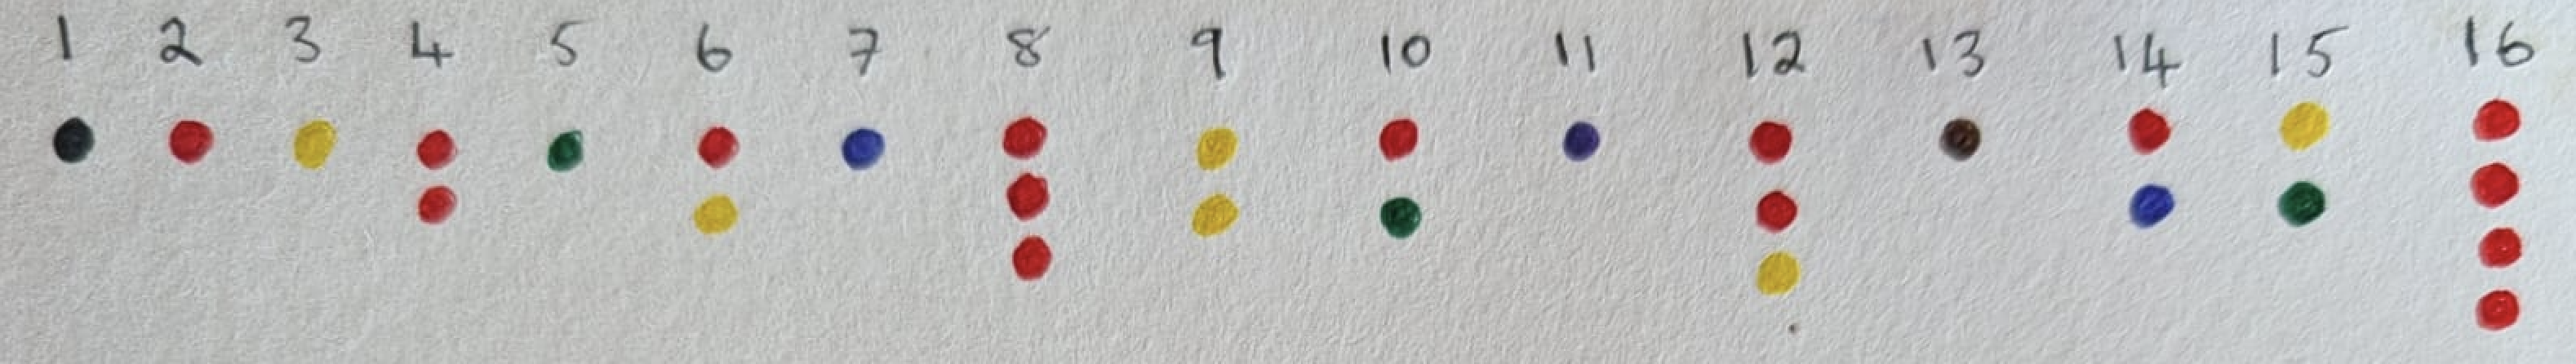
\includegraphics[width=400pt]{img/foundations--integers-e251.png}
  \end{mdframed}

 $c | a$, i.e. $c$ \defn{divides} $a$ ($a$ is a \defn{multiple} of $c$), i.e. if there exists $d$ such that $cd = a$.

 $\gcd(a, b)$, the \defn{greatest common divisor} of $a$ and $b$, is the largest integer $c$ such that $c | a$ and $c | b$.

  $a$ and $b$ are \defn{relatively prime} aka \defn{coprime} if $\gcd(a, b) = 1$.

  $\lcm(c, d)$ is the smallest integer $a$ such that $c|a$ and $d|a$.
\end{definition*}

  Question: why exactly are we contemplating products here, as opposed to e.g. sums?




\begin{remark*}
  a \defn{multiple} of a prime is a number whose factorization contains that prime.

  $c$ \defn{divides} $a$ ($a$ is a \defn{multiple} of $c$) if $a$'s factorization is a ``multiplicity superset​'' of $c$'s.

  The $\gcd$ is the largest integer whose factorization is a ``subset​'' of both factorizations.

  If $a$ and $b$ are relatively prime then their factorizations have no overlap.

  The $\lcm$ is the smallest integer whose factorization is a ``superset​'' of both factorizations.

  If $a$ is a multiple of $c$ then their $\lcm$ is $a$.

  If $a$ and $b$ are relatively prime then their $\lcm$ is their product.
\end{remark*}

\begin{example*}
Consider $2^2 \cdot 3 = 12$ and $2\cdot 3^2 = 18$.

Their factorizations have much in common (they are certainly not coprime), but neither is a
multiple of the other.

Their $\lcm$ is the first number that is a ``multiplicity superset​'' of the other: i.e. we must add
a factor of $3$ to $12$'s factorization, or an additional $2$ to $18$'s, either way
yielding $2^2 \cdot 3^2 = 36$.

Note that their $\lcm$ is not one of them (as it would be if one divided the other), but it is
smaller than their product.

The $\gcd$ of $2^2\cdot 3$ and $2\cdot 3^2$ is $2\cdot 3$.
\end{example*}


\begin{example*}
    For example if
  \begin{align*}
    a = 12 &= 2^2 \cdot 3 \\
    b = 40 &= 2^3 \cdot 5 \\
  \end{align*}
  then $\gcd(a, b) = 2^2 = 4$ and $\lcm(a, b) = 2^3 \cdot 3 \cdot 5 = 120$.

  This can be written as a general theorem involving mins and maxes in the exponents of a product
  of primes.
\end{example*}


\begin{theorem*}
  $\gcd(a,b) \times \lcm(a,b) = ab$
\end{theorem*}

\begin{example*}
  The product of  $2^2\cdot 3$ and $2\cdot 3^2$ is their concatenation: $2^2 \cdot 3 \cdot 2 \cdot 3^2 = 12 \cdot 18 = 216$.

  This is the product of their $\gcd$ $2\cdot 3$ and their $\lcm$ $2^2\cdot 3^2$.
\end{example*}


\begin{intuition*}
  We're performing additive operations on the exponents of the prime factors. The product is the
  sum of all; the $\gcd$ takes the min from each and is thus missing the maxes; the $\lcm$ takes
  the max from each and is thus missing the mins; their product contains the full multiplicities of
  all factors.
\end{intuition*}


\begin{theorem*}
  If $a|b$ then every prime factor of $a$ is a prime factor of $b$ and the associated exponent
  in $b$ is at least that in $a$.
\end{theorem*}

\begin{proof}
  By the Fundamental Theorem of Arithmetic any integer greater than $1$ can be written uniquely as
  a product of prime factors each raised to some exponent. The claim is true for $a=1$ so
  assume $a > 1$.

  Let $a = p_1p_2\cdots p_A$ and $b = q_1q_2\cdots q_B$ where $p_i$ and $q_j$ are prime for all
  $i = 1,2,\ldots,A$ and $j =1,2,\ldots,B$. Note that the $p$s and $q$s may have repeated values.

  Since $a|b$ we have $b = ka$ for some $k > 0$. Now suppose $p_i$ is a prime factor of $a$ that is not als

\end{proof}


\begin{theorem*}
  Let $a > 0$ and $b > 0$ with $a$ odd and $a | 2b$. Then $a | b$.
\end{theorem*}

\begin{proof}

  Since $a|2b$ we have $2b = ka$ for some $k > 0$


  Since $a|2b$ all the prime factors of $a$ are factors of $2b$. And since $a$ is odd, $2$ is not a
  factor of $a$. Therefore all the prime factors of $a$ are prime factors of $b$. Therefore $a|b$.
\end{proof}



\begin{mdframed}
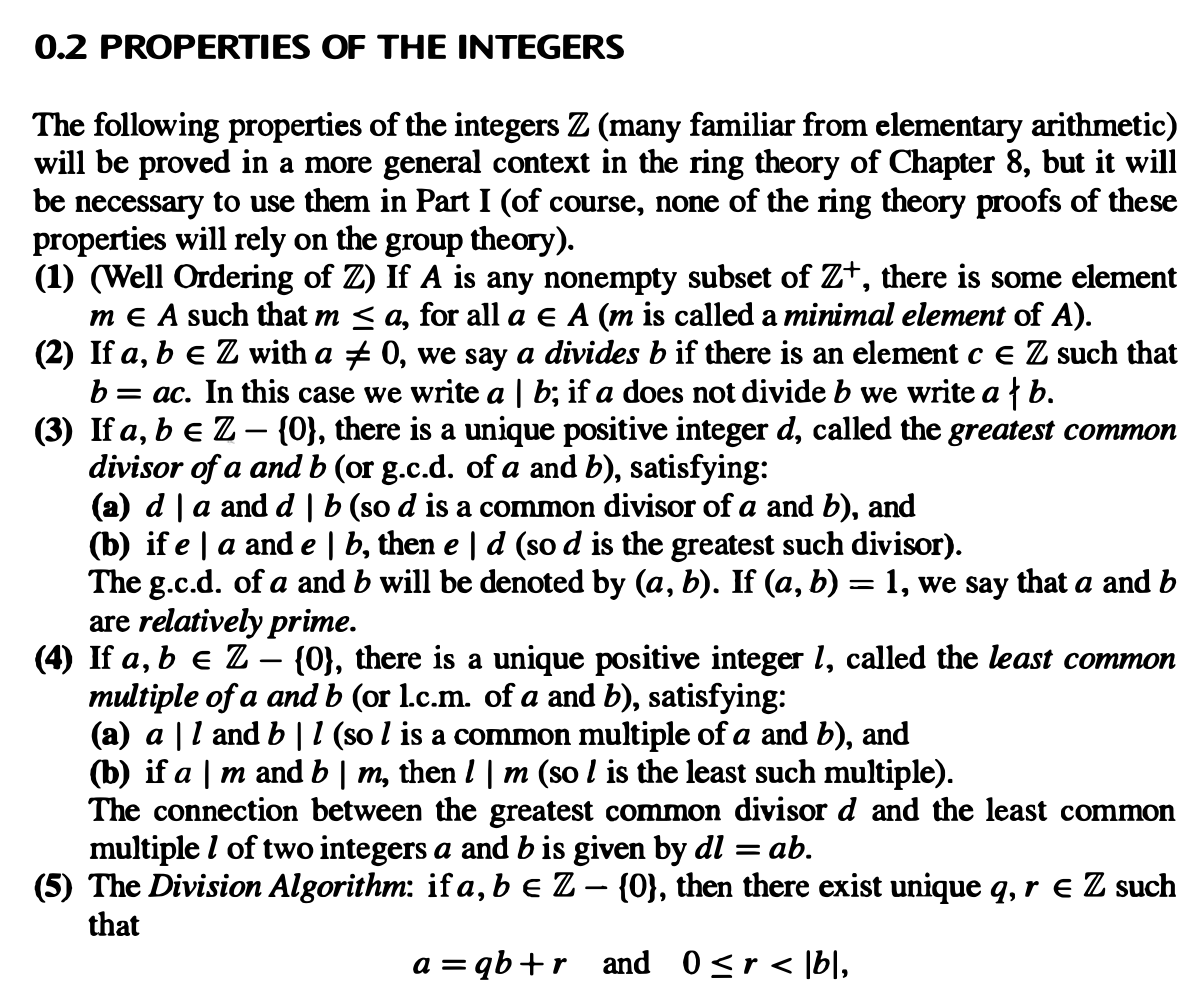
\includegraphics[width=400pt]{img/foundations--set-theory--number-theory-82fa.png}
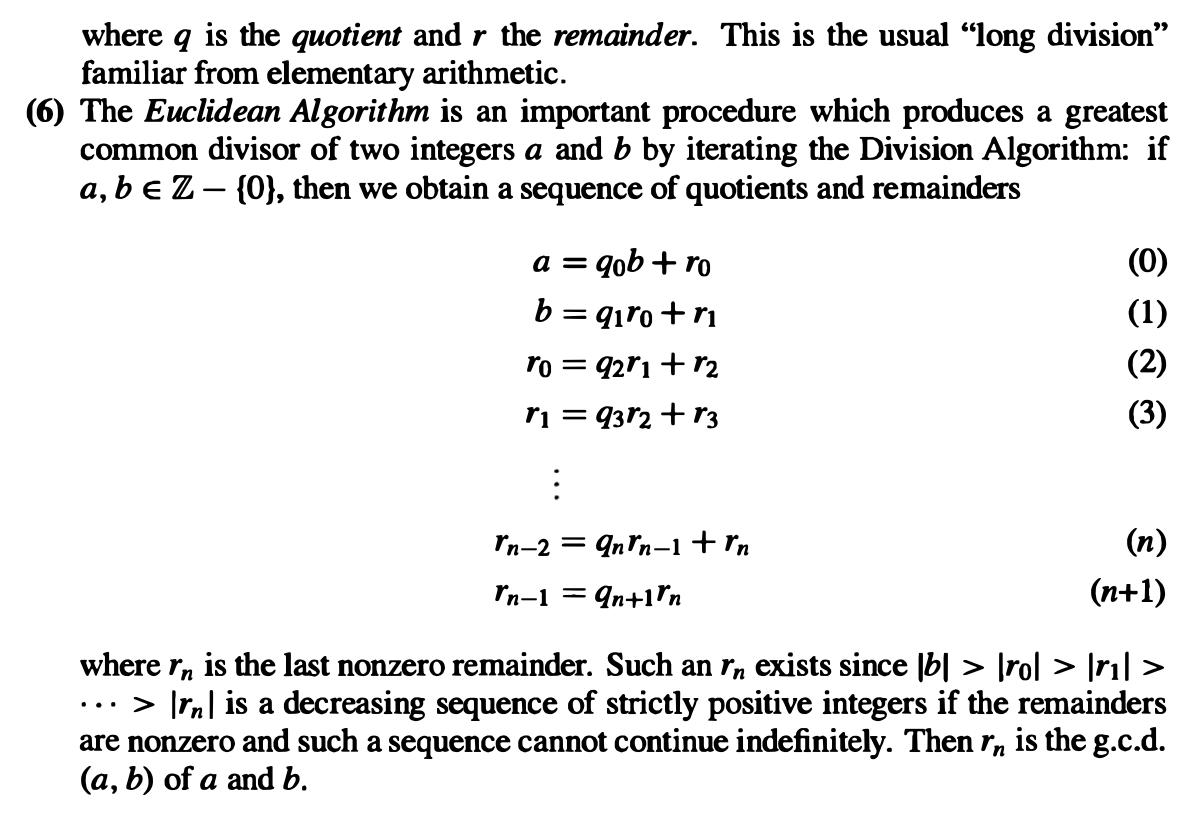
\includegraphics[width=400pt]{img/foundations--set-theory--number-theory-179a.png}
\end{mdframed}

\section{Set theory}

\begin{definition}[map, function]
  A \defn{map} (or \defn{function}) $f: A \to B$ is a subset of $A \times B$ such that each $a \in A$ has precisely one entry.

  $B^A$ is the set of maps $A \to B$.
\end{definition}

\begin{definition}[disjoint union]
  The \defn{disjoint union} of a collection of sets $\{A_i\}_{i \in I}$ is
  \begin{align*}
    \bigsqcup_{i \in I} A_i := \bigcup_{i \in I} \{(x_i, i) ~:~ x_i \in A_i\}.
  \end{align*}
  Note that (I think) we think of $A_i$ as being a subset of the disjoint union; the sets ``remain distinct​'' in
  the union.
\end{definition}

\begin{definition}[product]
  To be fully precise, the \defn{product} $\prod_{i \in I} A_i$ is the set of maps from $I$ to the disjoint union over
  the $A_i$s:
  \begin{align*}
    \prod_{i \in I} A_i := \(\bigsqcup A_i\)^I
  \end{align*}

  In other words, each element of this product is a pair $(i, (x, i))$.

  But usually one just thinks of each element as a pair $(i, x)$, where $x \in A_i$. So alternatively one can
  say that each element of the product is a sequence $(x_i)_{i \in I}$:
  \begin{align*}
    \prod_{i \in I} A_i := \{(x_i)_{i \in I} ~:~ x_i \in A_i\}.
  \end{align*}
\end{definition}

\begin{example}
  So $\R^3$ is the set of all ``functions from a 3-point index set into $\R$​'' (Murfet). Or equivalently,
  $\R^3$ is the set of all real-valued sequences of length $3$.

  This avoids us worrying about whether $\R^3$ is $\R \times (\R \times \R)$ or $(\R \times \R) \times \R$; it is neither.
\end{example}

\begin{definition}[power set]
The power set $\powerset(A)$ is the set of all subsets of $A$.

$\{0, 1\}^A$ means the set of all maps $A \to \{0, 1\}$. We have
\begin{align*}
  \powerset(A) \cong \{0, 1\}^A
\end{align*}
Each subset on the left has a corresponding characteristic function (indicator function) on the right.
\end{definition}


\section{Relations and partitions}
A relation on a set $A$ is a subset of $A^2$. Thus for a pair
$(a_1, a_2) \in A^2$ the relation says whether $a_1$ is related to $a_2$.

An equivalence relation is a relation that is reflexive, symmetric, and
transitive, and thus makes sense as defining a partitioning of the set into
groups of equivalent elements.

The equivalence relation doesn't tell you explicitly which group a pair belongs
to (it just tells you that they are in the same group). But the information is
there: the groups are the connected components in the graph in which two
vertices are connected if they are related. There are fewer equivalence
relations than assignments to labeled buckets, since the equivalence relation
does not identify the buckets. \blue{How many equivalence relations are there,
compared to Stirling II number and stars-and-bars count configurations?}

\begin{definition}
  Let $R \subseteq A \times A$ be a binary relation (arbitrary set of pairs). The \defn{equivalence relation generated by}
  $R$ is the intersection of all equivalence relations on $A$ that include $R$. This is the smallest
  equivalence relation containing that set of pairs.
\end{definition}




\section{Permutations and combinations}

\begin{theorem*}
  The number of $k$-tuples that can be formed from $\{1, 2, \ldots, n\}$ is
  \begin{align*}
    P(n, k) = n_{(k)} = n(n-1)(n-2)\cdots(n-k+1) = \frac{n!}{(n - k)!}.
  \end{align*}
  The number of sets of size $k$ that can be formed from $\{1, 2, \ldots, n\}$ is
  \begin{align*}
    C(n, k) = {n \choose k} = \frac{P(n, k)}{k!}.
  \end{align*}
\end{theorem*}

\section{Binomial theorem}
\begin{align*}
  (a + b)^n = \sum_{k=0}^n{n \choose k}a^{n-k}b^k
\end{align*}

\section{Taylor expansions}

Suppose that any function of a real number $f(x)$ can be represented by a "power series" with certain coefficients $c_i$
\begin{align*}
  f(x) = c_0 + c_1x^1 + c_2x^2 + c_3x^3 + c_4x^4 + ...
\end{align*}
Examining successive derivatives shows that $c_n = \frac{f^{(n)}(0)}{n!}$ (\red{TODO} explain why evaluating at zero).
For example, the Maclaurin expansion of $e^{x}$ is
\begin{align*}
  e^x = e^{0} + \frac{xe^0}{1!} + \frac{x^2e^0}{2!} + \cdots = \sum_{n=0}^\infty \frac{x^n}{n!}
\end{align*}

\section{Triangle inequalities}

\begin{theorem*}
  Let $a, b \in \R$ with $a \neq b$ and $a, b \neq 0$. Using $+$, $-$ and $|\cdot|$ we can generate the
  following 4 real numbers:
  \begin{align*}
    -\big(|a| + |b|\big) ~~~ < ~~~
    -\big||a| - |b|\big| ~~~ < ~~~
    0                    ~~~ < ~~~
    \big||a| - |b|\big|  ~~~ < ~~~
    |a| + |b|.
  \end{align*}
  \begin{itemize}
  \item $a + b$ and $a - b$ can equal any of them.
  \item $|a + b|$ and $|a - b|$ can equal either of the two positive numbers.
  \item $|a| - |b|$ can equal either of the two ``inner'' numbers.
  \end{itemize}
  ~\\~\\
  If we allow $a = b$ with $ a \neq 0, b \neq 0$ then
  \begin{align*}
    -\big(|a| + |b|\big) ~~~ < ~~~
    -\big||a| - |b|\big| ~~~ \red{\leq} ~~~
    0                    ~~~ \red{\leq} ~~~
    \big||a| - |b|\big|  ~~~ < ~~~
    |a| + |b|.
  \end{align*}
  If we allow $a = 0$ and $b = 0$ with $a \neq b$ then
  \begin{align*}
    -\big(|a| + |b|\big) ~~~ \red{\leq} ~~~
    -\big||a| - |b|\big| ~~~ < ~~~
    0                    ~~~ < ~~~
    \big||a| - |b|\big|  ~~~ \red{\leq} ~~~
    |a| + |b|;
  \end{align*}
  If we allow $a = b$ including $a = b = 0$ then
  \begin{align*}
    -\big(|a| + |b|\big) ~~~ \red{\leq} ~~~
    -\big||a| - |b|\big| ~~~ \red{\leq} ~~~
    0                    ~~~ \red{\leq} ~~~
    \big||a| - |b|\big|  ~~~ \red{\leq} ~~~
    |a| + |b|;
  \end{align*}
\end{theorem*}

\section{The quadratic formula}

\begin{theorem*}
  The roots of $ax^2 + bx + c = 0$ are $x = \frac{-b \pm \sqrt{b^2 - 4ac}}{2a}$.
\end{theorem*}

\begin{proof}
  \begin{align*}
    x^2 + \frac{b}{a}x + \frac{c}{a}                        &= 0\\
    \(x + \frac{b}{2a}\)^2 - \frac{b^2}{4a^2} + \frac{c}{a} &= 0 ~~~~~~~~~~~~~~~~~~~~~\text{``completing the square"}\\
    x &= -\frac{b}{2a} \pm \sqrt{\frac{b^2}{4a^2} - \frac{4ac}{4a^2}}\\
                                                            &= \frac{-b \pm \sqrt{b^2 - 4ac}}{2a}.
  \end{align*}
\end{proof}

\section{Geometric series}
\begin{theorem*}
  $a_n := \sum_{k=0}^nr^k = \frac{~~~~1 - r^{n+1}}{1 - r}$.

  Therefore if $r < 1$ then $\lim_{n \to \infty} a_n = \frac{1}{1 - r}$.
\end{theorem*}
\begin{proof}
  \begin{align*}
    a_n          &= \sum_{k=0}^nr^n = 1 + r + r^2 + \ldots + r^n\\
    a_n - ra_n  &= 1 - r^{n+1}\\
    a_n          &= \frac{~~~~1 - r^{n+1}}{1 - r}
  \end{align*}
\end{proof}
\begin{remark*}
  Note that $a_{n+1} = 1 + ra_n$.
\end{remark*}

\section{Partial fractions}

\red{TODO}

\section{Even and odd functions}

\begin{definition*}
  A function (over an additive group?) is even if $f(-x) = f(x)$ for all $x$.

  A function (over an additive group?) is odd if $f(-x) = -f(x)$ for all $x$.
\end{definition*}

Functions can be neither even nor odd.

\begin{claim*}
  A polynomial $p(x)$ is even if an only if it has only even powers of $x$.

  A polynomial $p(x)$ is odd if an only if it has only odd powers of $x$.
\end{claim*}

\section{Convex and concave functions}\label{convexity}
A real-valued function $f:\R\to\R$ is \defn{convex} over an interval $[x_1, x_2]$ if the line
segment joining $f(x_1)$ to $f(x_2)$ lies above the graph of $f$, i.e. if
\begin{align*}
  pf(x_1) + (1-p)f(x_2) \geq f(px_1 + (1 - p)x_2).
\end{align*}
E.g. $x \mapsto x^2$ and $x \mapsto e^x$ are convex.

A real-valued function $f$ is \defn{concave} if $-f$ is convex. These definitions extend to
real-valued functions $f$ over an $n$-dimensional interval / convex set\footnote{ Basically, a set
  which includes all points on line segments joining points in the set.}.

\section{Trigonometric identities}
\begin{align*}
  \cos 2\theta &= \cos^2\theta - \sin^2\theta
\end{align*}

\section{Hyperbolic trigonometric functions}\label{foundations-hyperbolic-trig-functions}

Define
\begin{align*}
  \cosh x &= \frac{e^x + e^{-x}}{2} \\
  \sinh x &= \frac{e^x - e^{-x}}{2}.
\end{align*}
Therefore
\begin{align*}
  \ddx \cosh x &= \sinh x \\
  \ddx \sinh x &= \cosh x,
\end{align*}
and
\begin{align*}
  \cosh^2 x             &= \frac{1}{4}\(e^{2x} + e^{-2x}\) + \frac{1}{2} \\
  \sinh^2 x             &= \frac{1}{4}\(e^{2x} + e^{-2x}\) - \frac{1}{2} \\
  1 + \sinh^2 x         &= \cosh^2 x \\
  \sinh^2 x + \cosh^2 x &= \cosh 2x
\end{align*}

$\sin$ and $\sinh$ are odd, and $\cos$ and $\cosh$ are even.

Note that these functions equal their own second derivatives. I.e. they provide solutions to
\begin{align*}
  \ddot{x} - x = 0.
\end{align*}
In contrast, $\sin$ and $\cos$ equal the negative of their own second derivative, so they provide
solutions to
\begin{align*}
  \ddot{x} + x = 0.
\end{align*}

\subsection*{\url{https://www.reddit.com/r/explainlikeimfive/comments/61siyw/eli5_can_someone_explain_the_hyperbolic_trig/}}

They are a bit mysterious, but not at all scary. It is just a way of grouping the exponential
functions into even and odd components.

From calculus, you know the relationship between the exponential and the standard trig functions:

\begin{align*}
e^{ix} = cos x + i sin x
\end{align*}

That works for imaginary arguments to the exponential and it splits it into a real and even
component (cosine) and an imaginary and odd component (sine). That is the solution to this
differential equation

\begin{align*}
  \ddot{y} + y = 0.
\end{align*}

Those functions are equal to the opposite sign of the second
derivative.

What about this differential equation:

\begin{align*}
  \ddot{y} - y = 0
\end{align*}

where the function is equal to its second derivative? Those solutions are simply $e^x$ and $e^{-x}$
. But neither of those solutions are even or odd. You could re-group those two solutions so that you
have an even solution and an odd solution.

\begin{align*}
e^x + e^{-x} &= (1/2) (e^x + e^{-x} ) + (1/2) (e^x - e^{-x} )
\end{align*}
They define the even solution to be hyperbolic cosine and the odd solution to be hyperbolic sine.

\begin{align*}
e^x + e^{-x} &= cosh x + sinh x
\end{align*}
So the definitions of the regular and hyperbolic trig functions with relation to the exponentials
are:

\begin{align*}
cos x &= (1/2) ( e^{ix} + e^{-ix} ) \\
sin x &= (1/2i) ( e^{ix} - e^{-ix} )
\end{align*}
and

\begin{align*}
cosh x &= (1/2) ( e^x + e^{-x} ) \\
sinh x &= (1/2) ( e^x - e^{-x} )
\end{align*}

You can see the analogy! From there, they can work out more algebra and calculus to see if there's
any other useful relations that make this splitting of the expontial into even and odd components
helpful. But it is not as crucial that you work with the hyperbolic functions this way. You could
choose to leave the solutions in their $e^{x}$ and $e^{-x}$ . Many times it helps, but its use is
not as common as the standard trig functions.


\begin{definition*}

 $c | a$, i.e. $c$ is a \defn{divisor} of $a$ (and $a$ is a \defn{multiple} of $c$), if there exists $d$ such that $cd = a$.

 $\gcd(a, b)$, the \defn{greatest common denominator} of $a$ and $b$, is the largest integer $c$ such that $c | a$ and $c | b$.

  $a$ and $b$ are \defn{relatively prime} aka \defn{coprime} if $\gcd(a, b) = 1$.

  $\lcm(c, d)$ is the smallest integer $a$ such that $c|a$ and $d|a$.
\end{definition*}

\begin{remark*}
  The $\gcd$ is the largest integer whose factorization is a ``subset​'' of both factorizations.

  If $a$ and $b$ are relatively prime then their factorizations have no primes in common.

  The $\lcm$ is the smallest integer whose factorization is a ``superset​'' of both factorizations.

  For example if
  \begin{align*}
    a = 12 &= 2^2 \cdot 3 \\
    b = 40 &= 2^3 \cdot 5 \\
  \end{align*}
  then $\gcd(a, b) = 2^2 = 4$ and $\lcm(a, b) = 2^3 \cdot 3 \cdot 5 = 120$.

  This can be written as a general theorem involving mins and maxes in the exponents of a product of primes.


\end{remark*}

\begin{theorem*}
  $\gcd(a,b) \times \lcm(a,b) = ab$
\end{theorem}


\section{$\sqrt{2}$ is irrational}
\begin{theorem*}
  $\sqrt{2}$ is irrational.
\end{theorem*}

\begin{proof}
  Suppose $\sqrt{2} \in \Q$. Then $\sqrt{2}$ can be written as $\frac{a}{b}$ where $a, b \in \Z$ are relatively prime.

  Then $2 = \frac{a^2}{b^2}$, so $a^2$ is even.

  Therefore $a$ is even.

  Let $a = 2c$. Then $b^2 = \frac{4c^2}{2} = 2c^2$, so $b^2$ is even.

  Therefeore both $a$ and $b$ are even, which is a contradiction.

  Therefore $\sqrt{2} \notin \Q$.
\end{proof}

\begin{remark*}
  It remains to be proved that $\sqrt{2}$ exists in $\R$. See \ref{existence-of-root-2}.
\end{remark*}

\section{Misc}
\begin{mdframed}
  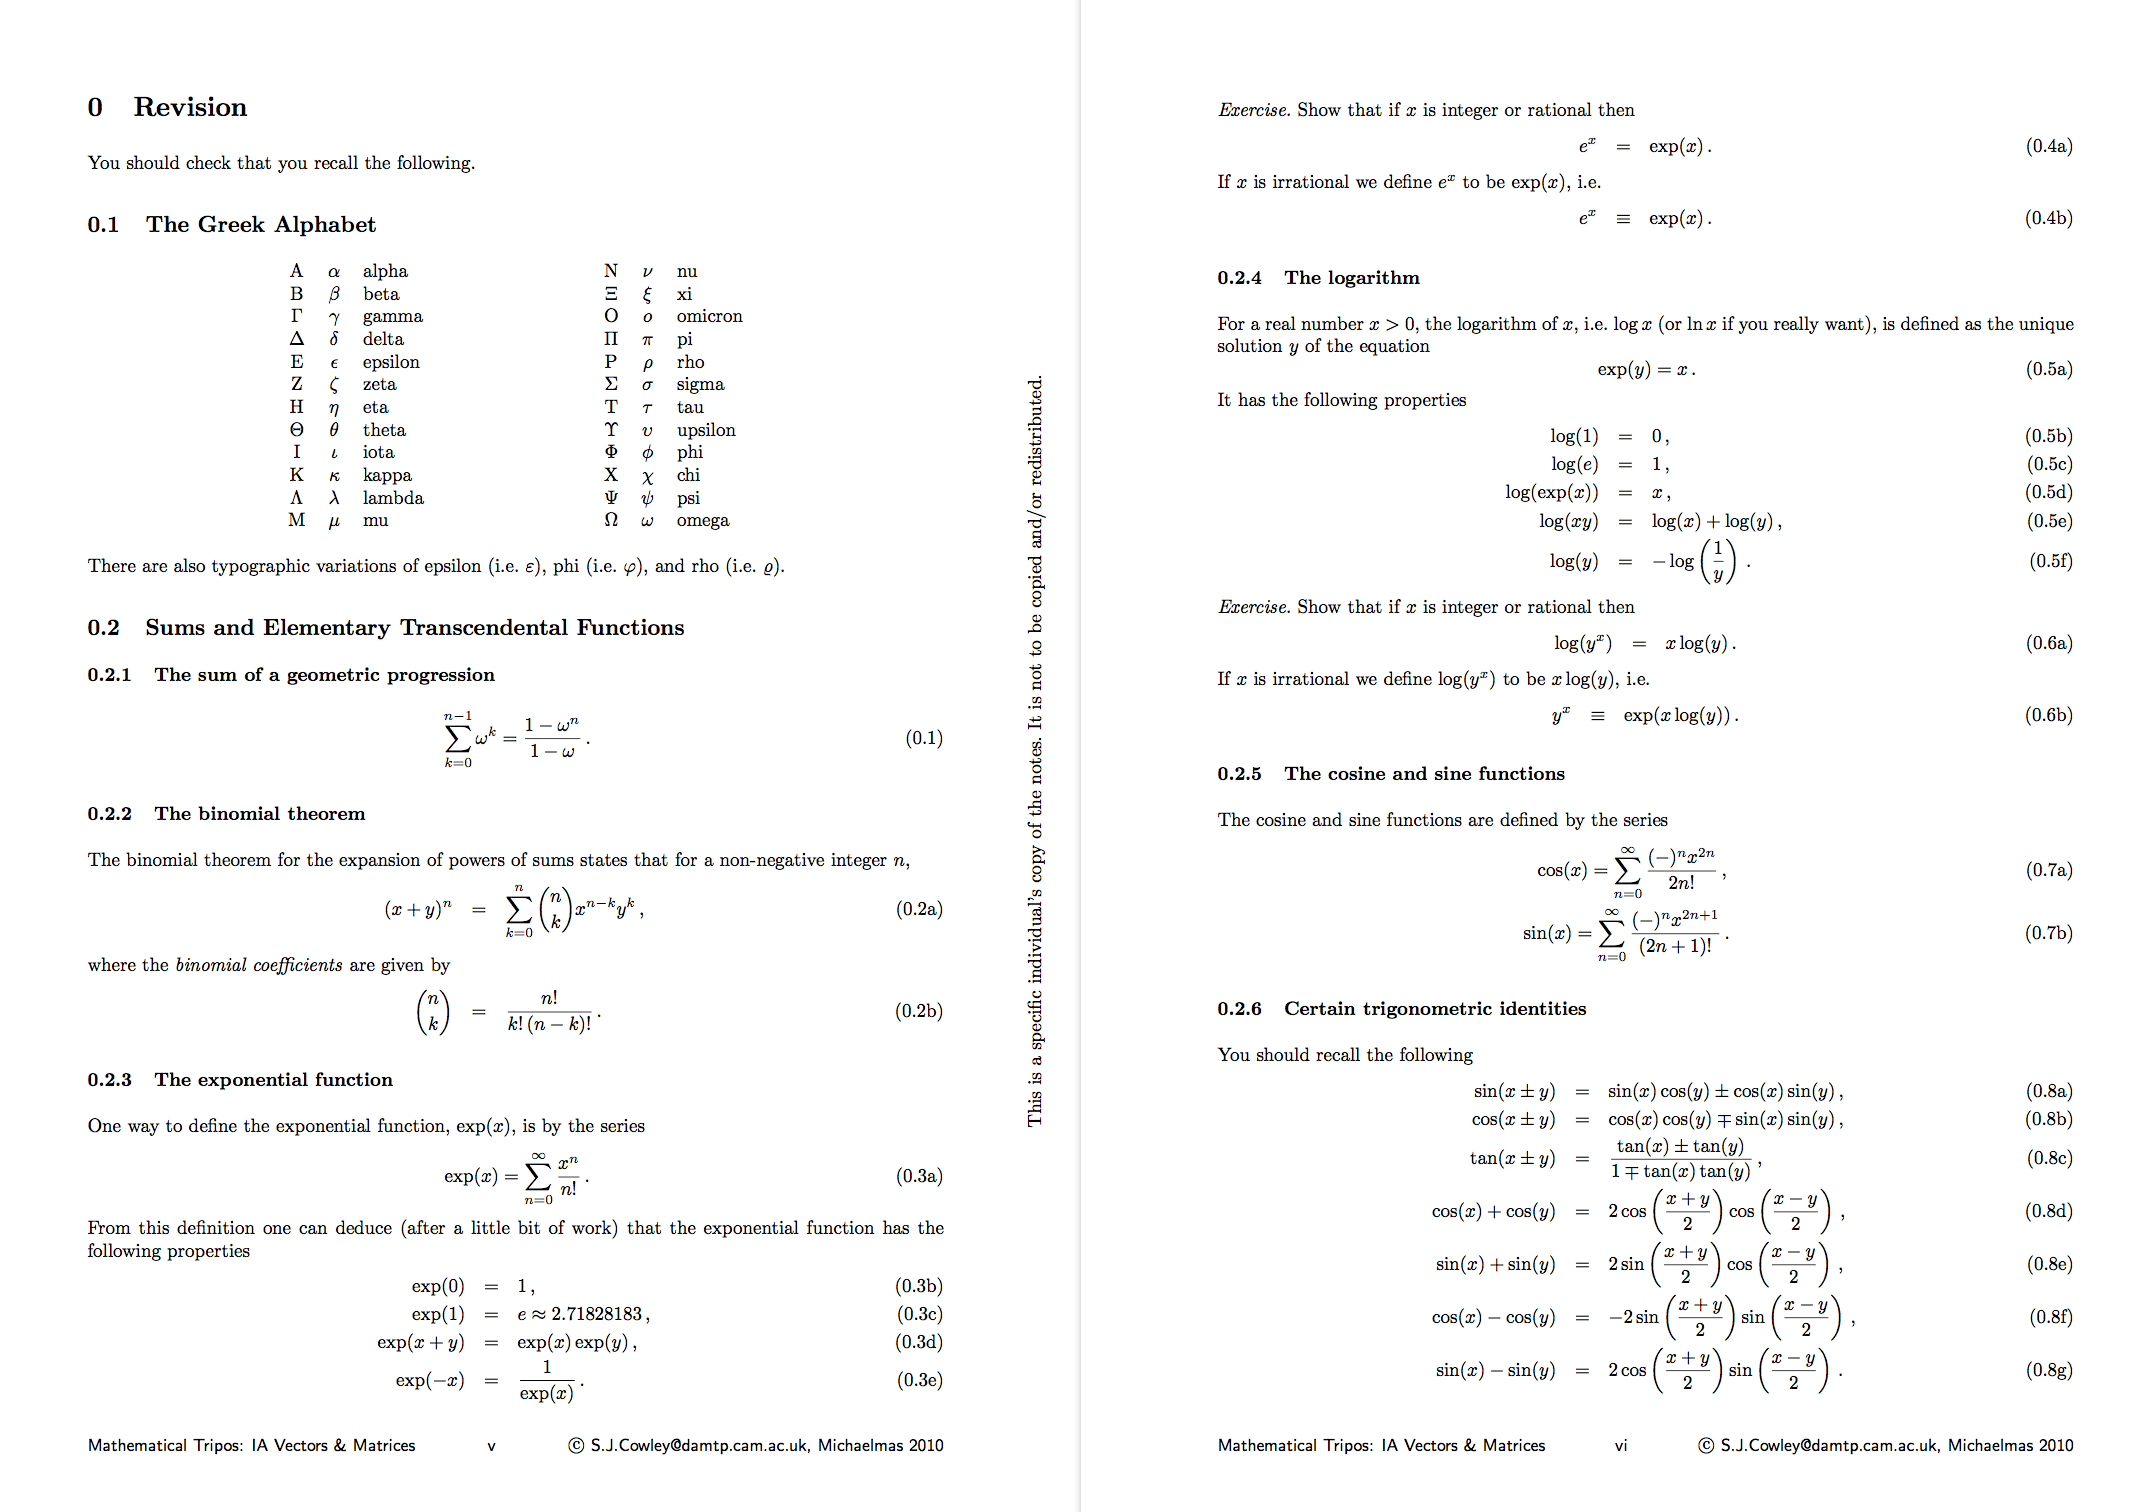
\includegraphics[width=400pt]{img/misc--cambridge-1a-vectors-and-matrices-revision-1.png}
\end{mdframed}
\begin{mdframed}
  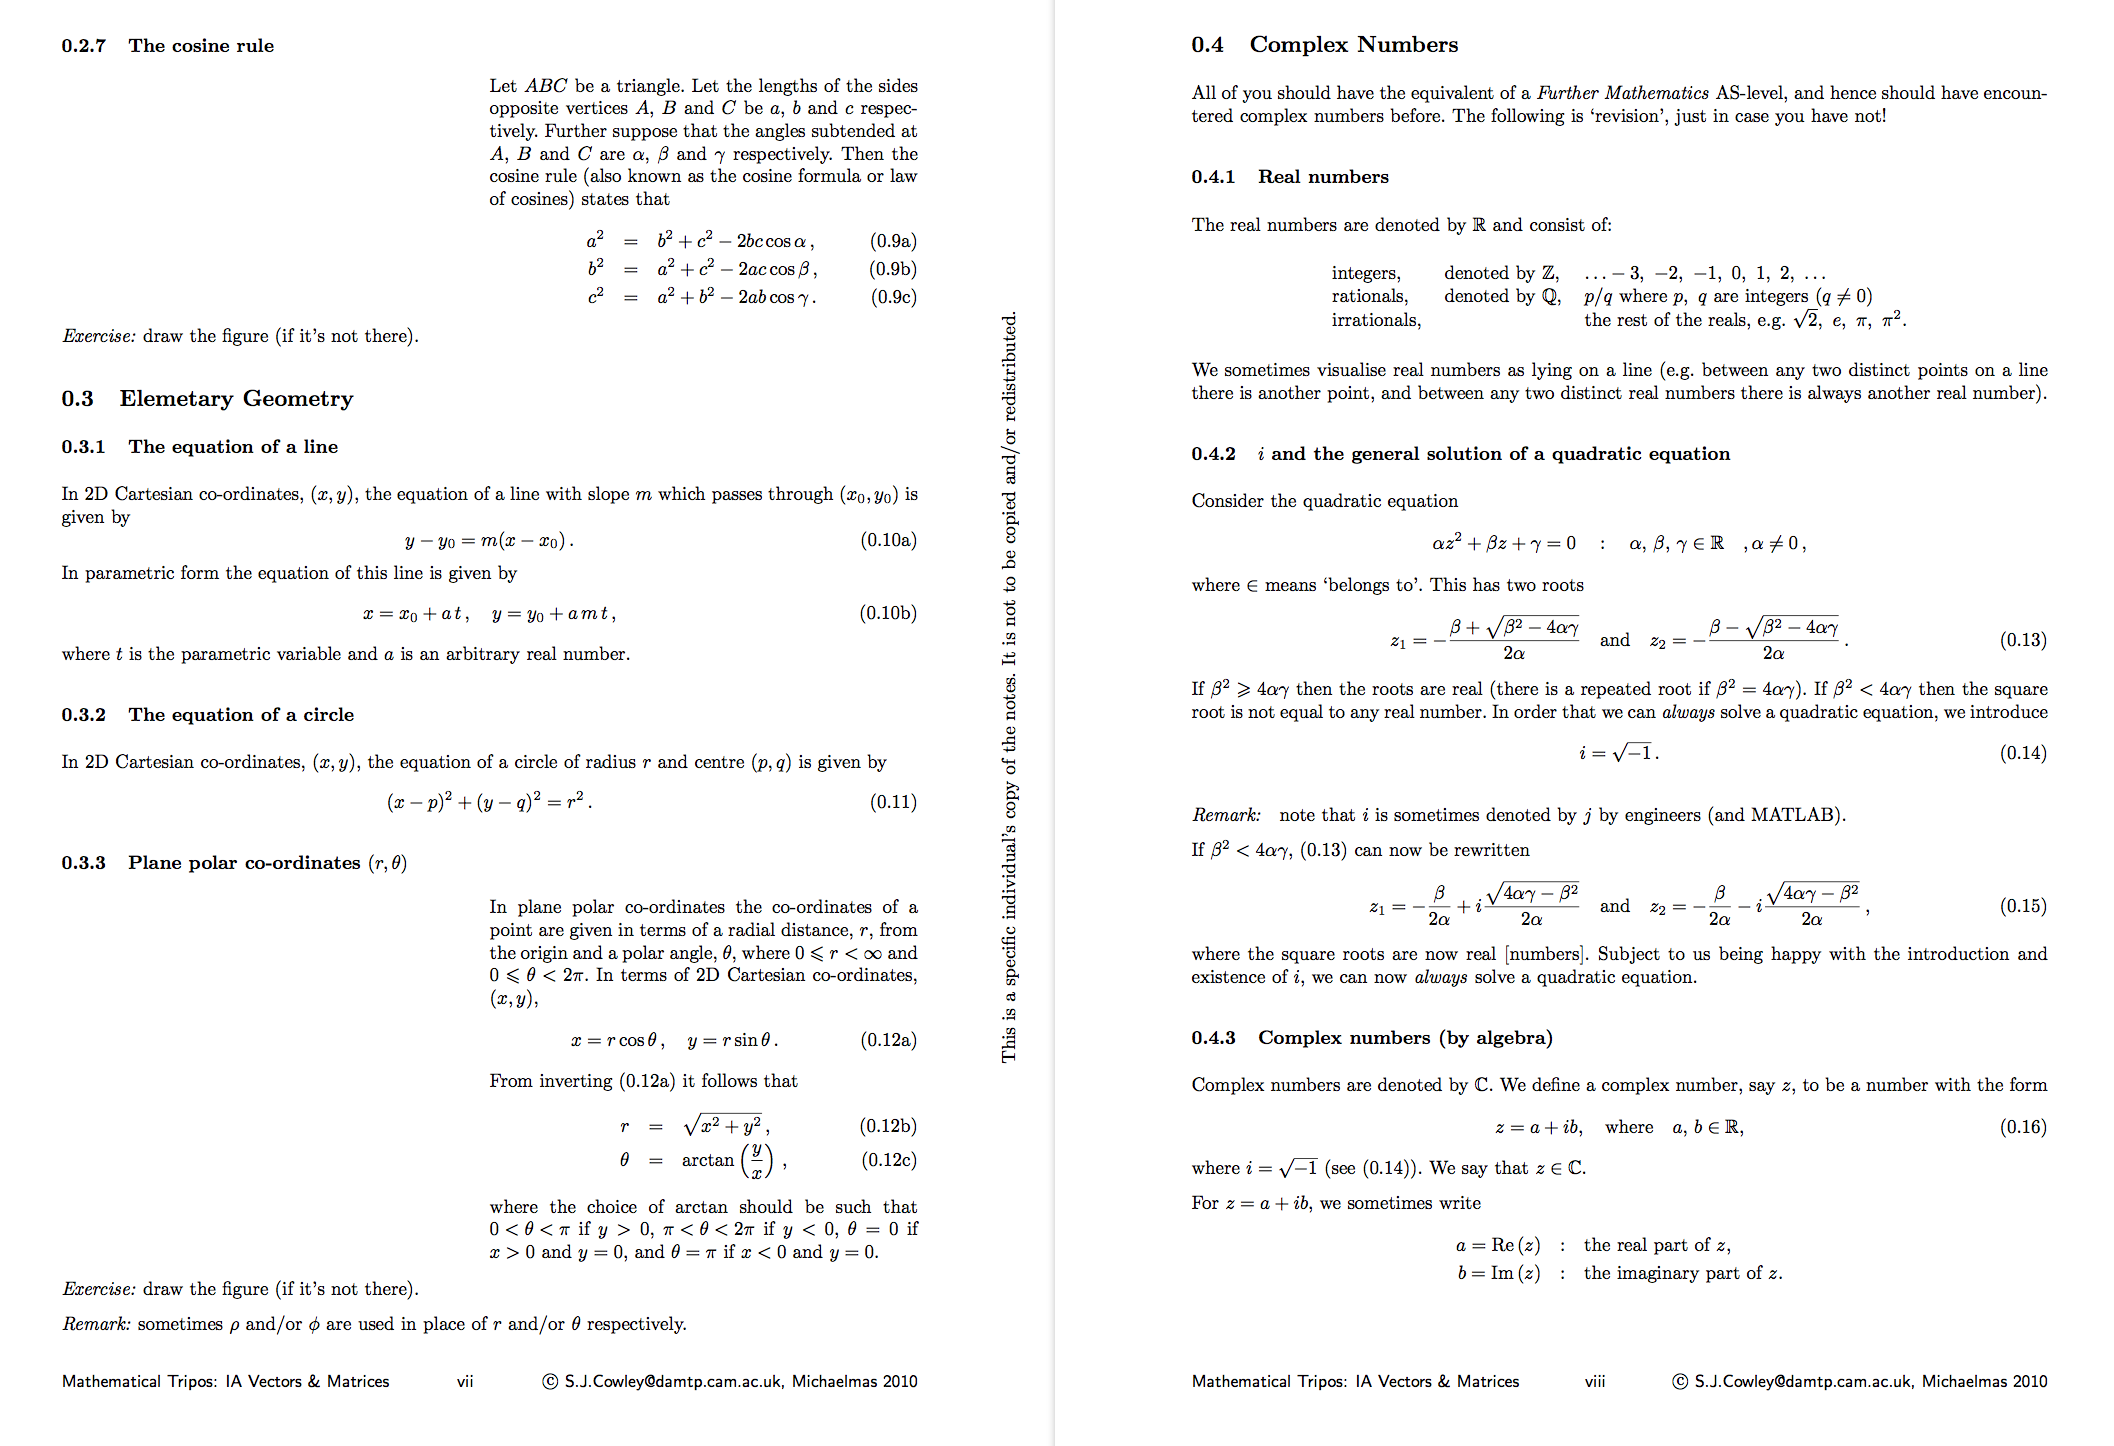
\includegraphics[width=400pt]{img/misc--cambridge-1a-vectors-and-matrices-revision-2.png}
\end{mdframed}
\begin{mdframed}
  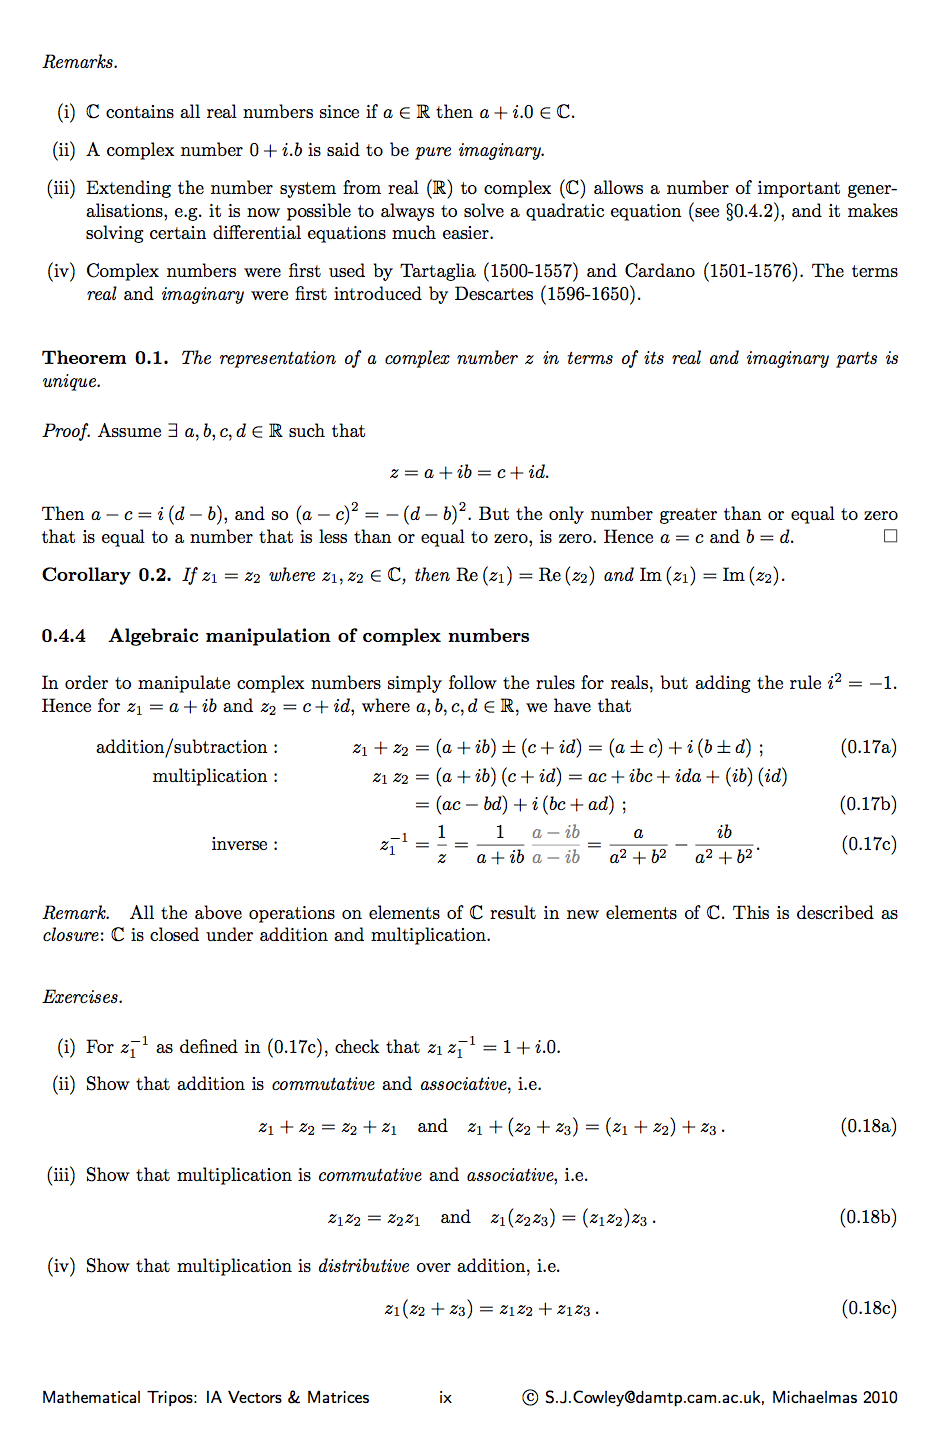
\includegraphics[width=400pt]{img/misc--cambridge-1a-vectors-and-matrices-revision-3.png}
\end{mdframed}


\begin{claim*}
  The sum of the first $n$ odd numbers equals $n^2$.
\end{claim*}

The claim is that $ = n^2$.

Note that by drawing patterns of dots we see that $\sum_{i=1}^n i$ can always be arranged to form
the upper triangle of a square, including the diagonal. Therefore
$\sum_{i=1}^n i = \frac{n^2 - n}{2} + n = \frac{n(n+1)}{2}$, and

\begin{align*}
  \sum_{i=1}^n (2i - 1)
  &= 2\sum_{i=1}^n i - n \\
  &= 2\frac{n(n+1)}{2} - n \\
  &= n^2.
\end{align*}


\chapter{Discrete Mathematics}

\section{Logic}
\subsection{Propositional logic}

\begin{definition*}
  An atom is a logical proposition which cannot be decomposed. A formula is a tree in which each
  node is either
  \begin{enumerate}
  \item an atom, or
  \item a logical operator with one child node for each argument.
  \end{enumerate}
  The logical operators are:
  \begin{itemize}
  \item $\lnot p$ negation
  \item $p \lor q$ disjunction
  \item $p \land q$ conjunction
  \item $p \limplies q$ implication
  \item $p \lequiv q$ equivalence
  \end{itemize}
  An interpretation is an assignment of true/false values to the atoms in a formula (well, except
  for logical constants, those are atoms but are constant true or constant false).

  A truth table is a list of all interpretations together with the resulting values of the formula.

  A model for a formula is an interpretation (row of truth table) for which the formula evaluates
  to true.

  A formula is satisfiable if there exists a model for it.

  A formula is valid (aka a tautology) if every interpretation is a model.

  The negation of a valid formula is not satisfiable.
\end{definition*}


\begin{theorem*}
  All other logical
\end{theorem*}

\newpage
\section{Combinatorics}

\begin{mdframed}
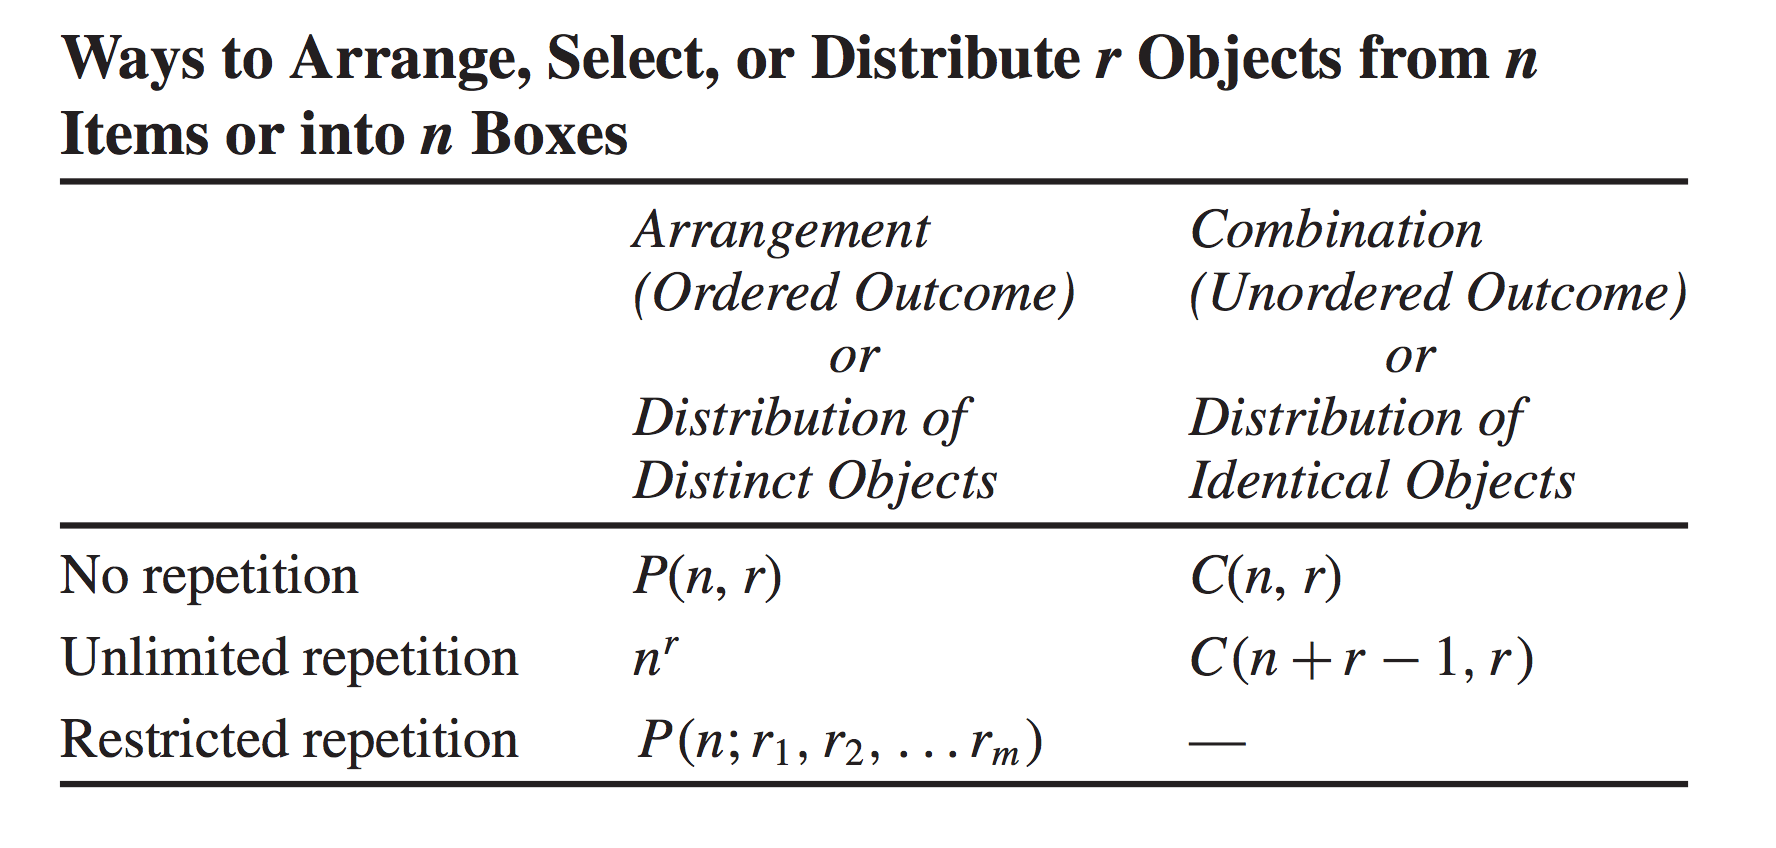
\includegraphics[width=300pt]{img/discrete-mathematics-tucker-combinatorics-summary.png}
\end{mdframed}

\begin{theorem*}[Subtuples]~\\
  The number of $k$-tuples that can be formed from a set of size $n$ without replacement is
  \begin{align*}
    (n)_k := n \cdot (n-1) \cdots (n - k + 1) = \frac{n!}{(n-k)!}.
  \end{align*}
\end{theorem*}

\begin{remark*}
  As a special case, the number of $n$-tuples (i.e. permutations/arrangements) is $n!$. (This is also
  the number of $n-1$ tuples.)
\end{remark*}

\begin{theorem*}[Subsets]~\\
  The number of subsets of size $k$ that can be formed from a set of size $n$ is
  \begin{align*}
    C(n, k) = {n \choose k} := \frac{(n)_k}{k!} = \frac{n!}{(n-k)!~k!}.
  \end{align*}
\end{theorem*}

\begin{proof}
  Each distinct $k$-subset gives rise to $k!$ $k$-tuples by assigning position labels. Therefore
  $(n)_k = {n \choose k}k!$.
\end{proof}

\begin{theorem*}[Multiset arrangements]~\\
  Consider a multiset comprising $n$ distinct elements, with $r_i \geq 1$ repeats of the $i$-th
  element. The number of $n$-tuples that can be formed from such a multiset is
  \begin{align*}
    P(n; r_1, \ldots, r_k)
    :=& {n \choose r_1}{n - r_1 \choose r_2}\cdots{n - r_1 \cdots - r_{n-1} \choose r_n}\\
    % &=\frac{n!}{(n - r_1)!r_1!}
    %   \frac{(n - r_1)!}{(n - r_1 - r_2)!r_2!}
    %   \cdots
    %   \frac{(n - r_1 \cdots - r_{n-1})!}{r_n!}
     =& \frac{n!}{r_1!r_2!\cdots r_n!}.
  \end{align*}
\end{theorem*}

\begin{proof}
  The $r_1$ copies of the first element must all go somewhere. ${n \choose r_1}$ counts the number
  of distinct positions they can occupy. Then there are $n - r_1$ empty positions left. Etc.
\end{proof}

\begin{remark*}
  The number $n!$ of permutations of a set is a special case of this with $r_i = 1$ for all $i$.
\end{remark*}

\begin{example*}~\\
  \begin{enumerate}
  \item {\bf How many ways are there to assign 100 different diplomats to five different
      continents?}\\
    $5^{100}$
  \item {\bf How many ways if 20 diplomats must be assigned to each continent?}\\
    $P(100; 20, 20, 20, 20, 20)$. Arrange the 100 diplomats in an arbitrary order. Now we have a
    multiset of country labels with 20 repeats of each label. Given the fixed ordering of the
    diplomats, there's a one-to-one correspondence between distinct permutations of the multiset
    and assignments of diplomats to countries.
  \item {\bf How many ways are there to distribute 20 (identical) sticks of red licorice and 15
    (identical) sticks of black licorice among five children?}\\
  ${20 + 5 -1 \choose 5 - 1}$${15 + 5 -1 \choose 5 - 1}$.
  \end{enumerate}
\end{example*}

\begin{theorem*}
  How many $k$-tuples for $k \leq n$ can be formed from such a multiset?
\end{theorem*}
\red{TODO}

\begin{theorem*}[Stars and bars]~\\
  Consider the number of ways that $n$ identical objects can be put into $k$ buckets, recording
  only the counts in each bucket (not the identities of the objects).

  With no empty buckets, the answer is
  \begin{align*}
    {n - 1 \choose k - 1} ~~~~~~~\text{($k-1$ bars to be placed in $n-1$ gaps between $n$ stars)}.
  \end{align*}

  With empty buckets allowed, the answer is
  \begin{align*}
    {n + k - 1 \choose k - 1} = P(n + k - 1; n, k - 1)~~~~~~~\text{(number of arrangements of $n$ stars and $k-1$ bars)}.
  \end{align*}
\end{theorem*}

\begin{proof}
  Represent this as $n$ unlabeled stars, and $k-1$ bars representing the partition of the stars
  into different buckets.

  With no empty buckets allowed, there are $n-1$ gaps where the bars can be placed, hence
  ${n - 1 \choose k - 1}$ ways of dividing up the items.

  With empty buckets allowed, there could be multiple bars in the same position. The number of
  $(n + k - 1)$-tuples that can be formed from the star and bar symbols is
  \begin{align*}
    P(n + k - 1; n, k - 1) &= C(n + k - 1, k - 1)C(n, n)\\
                           &= C(n + k - 1, k - 1)\\
                           &= C(n + k - 1, n)C(k - 1, k - 1)\\
                           &= C(n + k - 1, n).
  \end{align*}

  Note that ${n - 1 \choose k - 1}$ for the no-empty-buckets version can also be derived as
  follows:
  \begin{enumerate}
  \item Place one item into each bucket.
  \item Now there are $n - k$ items into $k$ buckets and empty buckets are allowed for the
    subsequent allocations. So the answer is
    ${(n - k) + k - 1 \choose k - 1} = {n - 1 \choose k - 1}$ by the empty-buckets-allowed theorem.
  \end{enumerate}
\end{proof}

\begin{theorem*}[Stars and bars]~\\
  The number of ways that $n$ items can be put into $k$ buckets, with empty buckets allowed,
  recording only the counts in each bucket (not the identities of the items), is

\end{theorem*}

\begin{theorem*}[Partitions]~\\
  The number of ways that $n$ items can be put into $k$ buckets, with no empty
  buckets, recording the identities of the items in each bucket, is the number of
  \textit{partitions} of size $k$ of a set of size $n$. It is equal to the
  Stirling number of the second kind:
  \begin{align*}
    S(n, k) = \frac{1}{k!} \sum_{i=0}^k(-1)^i{k \choose i}(k-i)^n. ~~ \blue{\text{(check this)}}
  \end{align*}
\end{theorem*}

\begin{proof}
  \red{TODO}
\end{proof}

\begin{claim}
  Consider the assignment of $n$ items $x_1, x_2, \ldots, x_n$ to $k$ buckets. Define $S_i$ to be the sum of items assigned to bucket $i$. The assignments for which $\max_i S_i$ is minimized is the assignment for which $\Var S_i$ is minimized.
\end{claim}

Not true?

\begin{theorem*}[Identities]~\\
  \begin{align*}
    {m + n \choose r} = \sum_{i=0}^r {m \choose i}{n \choose r - i}
  \end{align*}
\end{theorem*}

\subsection{Tucker - Applied Combinatorics - Exercises}

\begin{enumerate}
\item[(5.1)] {\bf General Counting Method for Arrangements and Selections}
  \begin{enumerate}
  \item[(37)] {\bf If three distinct dice are rolled, what is the probability that the highest
      value is
      twice the smallest value?}\\~\\
    $\frac{(3 \times 2 \times 3) + (3 \times 3!)}{6^3}$\\~\\
    An outcome is a 3-tuple such as $(1,1,1)$. Outcomes that match the criterion belong to two
    disjoint subsets:
    \begin{enumerate}
    \item Outcomes with two distinct values, such as $(1,1,2)$. There are $3 \times 2 \times 3$
      such outcomes ($3$ choices of unordered pairs of numbers, each with two alternative labelings
      and $3$ distinct permutations).
    \item Outcomes with three distinct values, such as $(2,3,4)$. There are $3 \times 3!$ such
      outcomes ($1 + 2$ unordered triples of numbers, each with $3!$ distinct permutations)
    \end{enumerate}
  \end{enumerate}
  \newpage
\item[(5.2)] {\bf Simple arrangements and selections}
  \begin{enumerate}
  \item[(Example 2)] {\bf How many ways are there to arrange the 7 letters of the word SYSTEMS...}
    \begin{enumerate}
    \item {\bf ...?}\\
      \begin{align*}
        7_{(7 - 3)} = 7\cdot 6\cdot 5\cdot 4 ~~~~~~~\text{(Choose positions of the other 4 letters, then Ss determined.)}
      \end{align*}
    \item {\bf ...with the 3 Ss consecutive?}
      \begin{align*}
        5_{(5)} = 5! ~~~~~~~\text{(Consider as 5-letter word S$^3$YTEM.)}
      \end{align*}
    \item {\bf ...with E before M?}
      \begin{align*}
        {7 \choose 2}5_{(5 - 3)} = {7 \choose 2}5\cdot 4 ~~~~~~~\text{(Choose position of E,M, then choose position of non-Ss.)}
      \end{align*}
    \item {\bf ...with E before M and 3 Ss consecutive?}
      \begin{align*}
        {5 \choose 2} 3! ~~~~~~~\text{(Consider as 5-letter word S$^3$YTEM, choose position of E,M, then choose positions for remaining letters.)}
      \end{align*}
    \end{enumerate}
  \item[(Example 6)] How
  \end{enumerate}
\end{enumerate}


\subsection{Generating functions}

\begin{definition*}[Generating function]
  Let $a_r$ be the number of ways to select $r$ objects in some counting procedure. Then $g(x)$ is
  a generating function for $a_r$ if $g(x)$ has the polynomial expansion
  \begin{align*}
    a_0 + a_1x + \ldots + a_nx^n.
  \end{align*}
\end{definition*}


\begin{example*}
  Find the generating function for $a_r$, the number of ways to select $r$ balls from $3$ green,
  $3$ white, $3$ blue, and $3$ gold balls.


\end{example*}

\newpage
\section{Pythagorean triples}

\subsection*{Project Euler question 9}

\begin{mdframed}
  A Pythagorean triplet is a set of three natural numbers, $a < b < c$, for which
  $a^2 + b^2 = c^2$.  For example, $3^2 + 4^2 = 9 + 16 = 25 = 5^2$.

  There exists exactly one Pythagorean triplet for which $a + b + c = 1000$.  Find the product
  $abc$.
\end{mdframed}

\begin{proof}~\\
  Let $m, n \in \N$.

  Recall that $|m + ni| := \sqrt{m^2 + n^2}$ and that $|wz| = |w| |z|$ for $w, z \in \C$.

  Note that $|(m + ni)^2| = |(m^2 - n^2) + 2mni| = m^2 + n^2 \in \Z$.

  Therefore $(m^2 - n^2, 2mn, m^2 + n^2)$ is a pythagorean triple for all $m, n \in
  \N$. (Claim: all pythagorean triples are of this form.)

  Therefore we seek $m, n \in \Z$ such that $m > n$ and
  \begin{align*}
    m^2 - n^2 + 2mn + m^2 + n^2             &= 1000\\
    m^2 + mn                                &= 500\\
    \(m + \frac{n}{2}\)^2 - \frac{n}{4} - 500 &= 0\\
    m                                       &= \sqrt{\frac{n}{4} + 500} - \frac{n}{2}
  \end{align*}
  Therefore (?) $\sqrt{\frac{n}{4} + 500} \in \Z$. So $\frac{n}{4} + 500 = a^2$
  for some $a \in \Z$.


\end{proof}


\chapter{Abstract algebra}
\newcommand{\alphainv}{\alpha^{-1}}

\section{Group, Homomorphism}
A group is a set, together with an operation that can be performed on two
elements to produce another element.

Concrete examples of groups:

- $\{1, i, -1, -i\}$ where the operation is multiplication of complex numbers.

- $GL_n(\R)$: the set of $n \times n$ matrices, under matrix multiplication.

- $S_2$: the set of permutations of two objects, where the operation is
  composition of functions.  There are just two elements in the group: the
  do-nothing permutation and the switch-the-elements permutation: $\{e,
  \tau\}$.

- $S_3$: the set of permutations of three objects. There are 6 elements: the
  identity, 3 transitions[ref]A transition is a permutation that switches two
  elements and leaves all other alone[/ref] and two cyclic permutations.

A \textbf{homomorphism} is a map\footnote{"map" is a synonym of "function".} from
one group to another. If it is bijective, it is an \textbf{isomorphism}. If it is
bijective and from a group to itself (i.e. a permutation of the group elements)
then it is an \textbf{automorphism}. The critical feature of these concepts is that
they "preserve group structure", i.e. they preserve the relationships among
group elements defined by the group operation. Suppose that they map from group
$G$ to group $G'$. Then the preservation-of-structure criterion is that the map
sends a product $g_1 \circ g_2$ to the product of whatever the separate
elements are sent to:

$$
f(g_1 \circ g_2) = f(g_1) \circ f(g_2)
$$

There the composition on the left is happening in $G$ and the composition on
the right is happening in $G'$. (For an automorphism, $G=G'$.)

Note that an element such as $g_1$ that is being sent somewhere by a morphism
may itself already be a map of sorts, e.g. if it is a permutation in
$S_3$. This is potentially confusing, since an automorphism can be thought of
as a permutation of group elements. So an automorphism on $S_3$ is a
permutation of group elements that are themselves permutations of some generic
labeled objects.

The definition of homomorphism implies that $f(g^{-1}) = f(g)^{-1}$ since
$f(gg^{-1}) = f(g)f(g^{-1}) = f(e)$.

\section{Kernel, Nullspace, Bijection and Congruency}

Consider a homomorphism $f$ with kernel $N$.

\textbf{Theorem:} $a$ and $b$ are sent to the same place by $f$ if and only if
$b = an$ for some $n \in N$.

\textbf{Corollary:} $f$ is a bijection (isomorphism) if and only if the kernel
contains only the identity element.

\textbf{Example:} Consider the absolute value homomorphism mapping complex numbers
under multiplication to positive reals under multiplication. The equivalence
classes are concentric circles around the origin. Two complex numbers have the
same absolute value iff one can be obtained from the other by rotation only (no
scaling). This is multiplication by a complex number with absolute value 1, and
such a complex number is in the kernel.

\textbf{Proof:} Clearly, if $b = an$ then $b$ is sent to the same place as $a$,
since

$$
f(b) = f(an) = f(a)f(n) = f(a).
$$

However we need to demonstrate the converse, i.e. that the *only* way that $b$
can be sent to the same place as $a$ is if $b=an$ for some $n \in N$.

Two almost identical ways of showing that:

\textbf{(1) Show that if $f(a) = f(b)$ then $b = an$ for some $n \in N$}

In linear algebra, you can always get from $u$ to $v$ by adding $v - u = -u +
v$, so the claim is that $L(u) = L(v)$ implies $-u + v$ is in the nullspace,
which is true:

$$
L(-u + v) = L(-u) + L(v) = L(-u) + L(u) = 0.
$$

For a group homomorphism, $b$ can be written as $aa^{-1}b$, so the claim is
that $f(a) = f(b)$ implies $a^{-1}b \in N$, which is true:

$$
f(a^{-1}b) = f(a^{-1})f(b) = f(a)^{-1}f(a) = e.
$$

\textbf{(2) Show that if it is not the case that $b = an$ for some $n \in N$, then $f(a) \neq f(b)$}

In linear algebra, you can always get from $u$ to $v$ by adding $v - u = -u + v$,
so if $-u + v$ is not in the nullspace then

$$
L(v) = L(u + (-u + v)) = L(u) + L(-u + v) \neq L(u).
$$

For a group homomorphism, $b$ can be written as $aa^{-1}b$, so if $a^{-1}b$ is
not in the kernel then

$$
f(b) = f(aa^{-1}b) = f(a)f(a^{-1}b) \neq f(a)
$$


\section{Inverse of an automorphism is an automorphism}

[Artin 2.3.11: show that Aut($G$) is a group]

Suppose $\alpha$ is an automorphism that sends $g_1$ and $g_2$ to $g_1'$ and
$g_2'$, respectively.

<img width="300 px" src="/notes/images/group-theory/inverse-of-automorphism-1.png" />

We need to show that $\alphainv$ preserves structure, i.e. that when $\alphainv$ acts
on an element which is a product, say $g_1'g_2'$, it sends it to the product of
whatever it send the individual factors to:

$$
\alphainv(g_1'g_2') = \alphainv(g_1')\alphainv(g_2').
$$


Firstly, we know that $\alphainv(g_1')$ and $\alphainv(g_2')$ exist, i.e. some elements
are taken to them by $a$, because $a$ is an automorphism and therefore
surjective. So we'll call those $g_1$ and $g_2$, and the equality we need to
demonstrate has become

$$
\alphainv(\alpha(g_1)\alpha(g_2)) = g_1g_2.
$$

Since $\alpha$ is an automorphism, it preserves structure, therefore
$\alpha(g_1)\alpha(g_2) = \alpha(g_1g_2)$. So,

$$
\alphainv(\alpha(g_1)\alpha(g_2)) = \alphainv(\alpha(g_1g_2)) = g_1g_2,
$$

as required.


\chapter{Linear Algebra}
\section{Vector spaces and fields}\label{real-and-complex-vector-spaces}
A vector in a vector space is just something which can be added to another vector from the vector
space, and scaled by a scalar from the associated field. A vector does not involve any numbers until
it is represented as a linear combination of basis vectors, using nunbers from the associated
field. So whether something is a ``real vector space'' or a ``complex vector space'' depends only on
the field. If the field is $\R$ it is a real vector space; if the field is $\C$ it's a complex
vector space. It doesn't make sense to ask whether the vectors themselves are real or complex.

A \defn{field} is a set which is an abelian group under both addition and multiplication.

A \defn{vector space} is an additive abelian group $X$, together with a field $F$, such that $X$ is
closed under linear combinations with scalars from the field $F$.

\subsubsection{Examples}

% TODO:
% \begin{itemize}
% \item clarify: is $\C$ a field or a vector space or both?
% \item What is a one-dimensional complex vector space?
% \end{itemize}

\begin{enumerate}
\item $\R$ is a field.

\item $\R^2$ is not a field; multiplication is undefined.

\item If we equip $\R^2$ with complex multiplication then this is the field called $\C$.

\item The additive abelian group $\R$, together with the field $\R$, is a one-dimensional vector space.

  {\bf Proof:} Let $x \in \R$ with $x \neq 0$. Then $\{x\}$ is a basis for $\R$, since every element of $\R$ can
  be expressed uniquely as a scalar multiple of $x$. So $\R$ is one-dimensional.

\item The additive abelian group $\R^n$, together with the field $\R$, is a vector space. It is $n$-dimensional.

\item The additive abelian group $\C$, together with the field $\R$, is a two-dimensional vector
  space. It is isomorphic to $\R^2$.

\item The additive abelian group $\C$, together with the field $\C$, is a one-dimensional vector space.

  {\bf Proof:} Let $z \in \C$ with $z \neq 0$. Then $\{z\}$ is a basis for $\C$, therefore $\C$ as a
  complex vector space is one-dimensional.
\end{enumerate}

\newpage
\section{Examples of vector spaces}
\begin{enumerate}
\item The set $\R^n$ of $n-$tuples of real numbers, under componentwise addition and componentwise
  multiplication by real scalars.
\item Complex numbers
  \begin{enumerate}
  \item $\C$ under addition with multiplication by scalars from $\C$ is a field, and therefore a
    vector space. It is one-dimensional ($1$ and $i$ are not linearly independent).
  \item The set $\C^n$ of $n-$tuples of complex numbers, under componentwise addition and
    componentwise multiplication by complex numbers.
  \item $\C$ under addition with multiplication by real scalars is equivalent to $\R^2$.
  \end{enumerate}
\item Matrices \& linear transformations:
  \begin{enumerate}
  \item The set $M_{m \times n}(\R)$ of $m\times n$ matrices is a vector space, under componentwise
    addition and multiplication by real scalars.
  \item The set $\mathrm{Hom}(V, W)$ of linear transformations from vector space $V$ to vector
    space $W$ is a vector space: for scalar $a$, define $(aT)(v) := a(T(v))$, and
    $(S + T)v := S(v) + T(v)$.
  \end{enumerate}
\item The set $\R_n[x]$ of polynomials of degree $\leq n$ is a real vector
  space.
\item The set $\R^X$ of real-valued functions on any set $X$ is a real vector
  space. Examples:
  \begin{enumerate}
  \item Let $[n] = \{1, 2, \ldots, n\}$. Note that the function space $\R^{[n]}$ is
    the same as $\R^n$ (both are sets of $n-$tuples of reals).
  \item Similarly, $\R^{[m]\times[n]}$ is the same as $M_{m \times n}(\R)$.
  \item $\R^\R$, the set of all functions $\R\to\R$.
  \item The set of continuous functions $\R \to \R$, and differentiable functions
    $\R \to \R$, under pointwise addition and pointwise scalar multiplication
    (from any field?).
  \item Set of solutions of a homogeneous linear ODE
  \end{enumerate}
\item Sequences $(a_n)$ of real numbers, under term-wise addition and term-wise
  scalar multiplication, form a vector space, identifiable with the function
  space $\R^\N$. Examples:
  \begin{enumerate}
  \item Set of convergent sequences
  \end{enumerate}
\item The set of solutions of a system of \textit{homogeneous} linear equations
  in $n$ variables is a subspace $V$ of $\R^n$. (Let $A$ be the matrix
  representing the system and let $u$ and $v$ be solutions. Then $Au = Av = 0$
  and $V$ is a subspace since $A(u + v) = Au + Av = 0$, and
  $A(\lambda u) = \lambda Au = 0$.)
\end{enumerate}

\section{Linear systems}

Consider the linear systems
\begin{align*}
  \begin{array}{cc}
    \begin{cases}
      x = 0\\
      y = 0
    \end{cases}
    ~~~~~~~~~~~~~~~~~~~~~~~~~~~~&
    \begin{cases}
      x - y = 0\\
      x + y = 1\\
      x - z = 0
    \end{cases}
  \end{array}
\end{align*}

A ``solution'' is an assignment of values to the $n$ variables which makes all
$m$ equations true.

In other words, we notice that the equations involve $n$ variables, and
consider the set of $n$-tuples
$S = \{(x, y, \ldots) ~|~ x, y, \ldots \in \R\}$.

The set of solutions is the subset of $S$ for which all the equations are true.

Geometrically, we think of the 2-tuple $(a, b)$ as a point in the $\R^2$
plane. Specifically, if our basis is $\vec e_1, \vec e_2$, then $(a, b)$ is the
point $a\vec e_1 + b\vec e_2$. We might imagine that the basis is the standard
orthogonal basis, but that's not necessary.

The linear equations define hyperplanes (lines, planes etc) in $S$.

The set of solutions is the intersection of these hyperplanes: another
hyperplane or the empty set.

So at this point, we do not treat the ambient space as a vector space (we're
not adding or scaling points), and neither the equation hyperplanes nor the
solution hyperplane, need be a subspace (since it need not contain the origin).

Next, we rewrite the linear system as a matrix applied to a vector, $Ax = b$:
\begin{align*}
  \begin{array}{cc}
    \mat{1}{0}
        {0}{1} \vecMM{x}{y} = \vecMM{0}{0}
    ~~~~~~~~~~~~~~~~~~~~~~~~~~~~~~~~~~~~~~~&
    \matMMMxNN{1}{-1}
              {1}{~~1}
              {1}{-1} \vecMM{x}{y} = \vecMMM{0}{1}{0}.
  \end{array}
\end{align*}

The equation coefficients are now represented by a linear transformation
$A:\R^n \to \R^m$.

This matrix equation is saying:
\begin{enumerate}
\item Let the $x$ coefficients be a vector $\vec a_1 \in \R^m$. And let the $y$
  coefficients be another vector $\vec a_2 \in \R^m$, and so on.
\item So now you have $n$ vectors spanning some subspace of $\R^m$.
\item Is $b$ in their span? If so, for what values of $x, y, \ldots$ does
  $x\vec a_1 + y\vec a_2 + \cdots = b$?
\end{enumerate}

From Frenkel's Multivariable Calculus lectures:

\begin{center}
  \begin{quote}
    \textit{The dimensionality of an object is equal to the dimensionality of the
      ambient space, minus the number of independent equations.}
  \end{quote}
\end{center}

So, basically, suppose there are $n$ variables. Then the solution set is a
subset (hyperplane) of $\R^n$, and

\begin{tabular}{c|c}
  Independent equations & Solution set\\
  \hline
  1                     & $(n - 1)$-dimensional hyperplane \\
  2                     & $(n - 2)$-dimensional hyperplane \\
  \vdots                & \vdots \\
  $n-1$                 & line \\
  $n$                   & point \\
  $n + 1$               & impossible \\
  \vdots                & \vdots
\end{tabular}

So when do we get no solutions? That's when
\begin{align*}
  &\text{the $n$ columns of $A$ do not span $\R^m$}\\
  \iff &\Rank A < \text{(number of equations)}\\
  \iff &\text{not all equations independent},
\end{align*}
and $b$ is not in their span.

In other words, suppose we have a linear system involving $n$ variables.

Suppose that all the $m$ equations are independent: full row rank.

Then $m \leq n$.

Now we introduce a dependent equation into the system.

\red{One error above is that its only the coefficients of the equation that
  we're considering when we say the rows are dependent/independent. So it's not
  correct to talk about ``independent equations''.}


\section{Subspaces}
A subspace $U$ of $V$ is a subset of $V$ for which
\begin{enumerate}
\item $0 \in U$
\item For any finite subset $U^* \subset U$, the set of all linear combinations
  of $U^*$ is also a subset of $U$.
\end{enumerate}

\section{Span, basis, dimension}
\begin{theorem}
  Every basis has the same size.
\end{theorem}

\begin{proof} Let $v_1, \ldots, v_n$ be a basis for a vector space $V$.


\end{proof}

\begin{theorem}
  A spanning set that is the same size as a basis is also a basis.
\end{theorem}

\begin{proof}
  Let $v_1, \ldots, v_n$ be a basis for a vector space $V$, and let
  $u_1, \ldots, u_n$ span $V$.

  We know that $v_1, \ldots, v_n$ are linearly independent and that if we
  remove any one of them they will cease to span.

  We want to show that $u_1, \ldots, u_n$ are linearly independent.

  Suppose, that the $u_i$ are not linearly independent and that
  $u_2, \ldots, u_n$ span $V$. Thus there are $n-1$ vectors in this spanning
  set. But the Steinitz Exchange Lemma states that if $v_1, \ldots, v_n$ are
  linearly independent and $u_1, \ldots, u_m$ span, then $n \leq m$. This
  contradiction proves that the $u_i$ are linearly independent.
\end{proof}

\begin{theorem}\label{transformed-basis-is-a-basis}
  Let $U, V$ be vector spaces, let $f:U \to V$ be an invertible linear map, and let
  $e_1, \ldots, e_n$ be a basis for $U$. Then $f(e_1), \ldots, f(e_n)$ is a basis for $V$.
\end{theorem}

\begin{proof}We need to show that the $f(e_i)$ are linearly independent and spanning.

  \begin{enumerate}
  \item {\bf Linear independence}\\
    Suppose $\sumin \lambda_if(e_i) = 0$.

    Therefore $f\(\sumin \lambda_ie_i\) = 0$ since $f$ is linear.

    Therefore $\sumin \lambda_ie_i = f^\1(0) = 0$, since the preimage of $0$ is $\{0\}$ for an
    invertible linear map.

    But the $e_i$ are linearly independent, therefore $\lambda_i = 0$ for all $i = 1, \ldots n$, as
    required.

  \item {\bf Spanning}\\
    Let $v \in V$.

    Then $v = f(u)$ for some $u \in U$, since $f$ is surjective.

    Therefore $v = f\(\sumin \lambda_ie_i\) = \sumin \lambda_if(e_i)$ for some
    $\lambda_1, \ldots, \lambda_n$, as required.

  \end{enumerate}
\end{proof}

\begin{problem*}
  If $u, v$ are linearly independent under one basis are they linearly independent under all choices of basis?
\end{problem*}

\section{Linear transformations and matrices}

A linear transformation is completely specified by

\begin{enumerate}
\item Some basis vectors $i$ and $j$
\item Where those basis vectors are taken to by the transformation.
\end{enumerate}

How the transformation affects any other point follows from those two pieces of
information.

So $i$ might be taken to $ai + bj$, and $j$ might be taken to $ci + dj$.
In this case we would use the following matrix to describe the
transformation:

$$
\mat{a}{c}
    {b}{d}
$$

Some examples are

$$
\begin{array}{ll}
\text{stretch by a in the i-direction} & \mat{a}{0}
                                             {0}{1}
\\\\
\text{stretch by a in the i-direction and shear right} & \mat{a}{b}
                                                             {0}{1}
\\\\
\text{rotate anticlockwise 90°} & \mat{0}{-1}
                                      {1}{ 0}
\end{array}
$$

Note that we haven't said what $i$ and $j$ are yet; they \textit{define} the
2-dimensional space that we're considering. But, we can think of them for now
as the usual orthogonal unit vectors in 2D space.

So the matrix tells us where the basis vectors have been taken to. Any other
vector $fi + gj$ is taken to wherever that is using the transformed basis
vectors:

$$
fi + gj \longrightarrow f\cvec{a}{b} + g\cvec{c}{d} = \cvec{fa + gc}{fb + gd}
$$


And that's how matrix multiplication is defined:

$$
\mat{a}{c}
    {b}{d} \cvec{f}{g} = \cvec{fa + gc}{fb + gd}
$$


A matrix represents a linear transformation by showing where the basis vector
are taken to.

\begin{theorem}
  The inverse of a 2x2 matrix is...
\end{theorem}

\section{Geometric interpretation of matrix operations}
\url{https://math.stackexchange.com/questions/37398/what-is-the-geometric-interpretation-of-the-transpose}
\url{https://math.stackexchange.com/questions/598258/determinant-of-transpose/636198#636198}


\section{Commutativity}
\subsection{Examples of transformations that don't commute}
Let $A$ be reflection around the first coordinate axis $\matMMxNN{1}{0}
                                                                 {0}{-1}$
and let $B$ be $90\deg$ anticlockwise rotation $\matMMxNN{0}{-1}
                                                         {1}{0}$.

Then $BA = \matMMxNN{0}{1}
                    {1}{0}
\neq  AB = \matMMxNN{0}{-1}
                    {-1}{0}$.

Note that $A^\1 = A = A^T$ and $B^\1 = \matMMxNN{0}{1}
                                               {-1}{0} = B^T$.

Therefore these are both orthogonal (unitary) matrices.


\section{Eigenvalues, eigenvectors, characteristic polynomial}

Let $V$ be a vector space and let $T:V \to V$ be a linear transformation.

\begin{definition*}[eigenvalue]
  $\lambda$ is an \textit{eigenvalue} of $T$ iff there exists \todo{non-zero?} $v \in V$ such that
  $Tv = \lambda v$.
\end{definition*}

\begin{definition*}[eigenspace]
  $E_\lambda = \{v ~|~ Tv = \lambda v\}$ is an \textit{eigenspace} of $T$.
\end{definition*}

\begin{definition*}[eigenvector]
  An \textit{eigenvector} is a non-zero element of an eigenspace.
\end{definition*}

\begin{definition*}[characteristic polynomial]
  The characteristic polynomial of $T$ is $\chi_T(x) = \det(T - xI)$. Note that
  $\lambda$ is an eigenvalue of $T$ iff $x=\lambda$ is a root of $\chi_T(x)$.
\end{definition*}

\begin{intuition*}~\\
  Decompose $T$ as the sum of two transformations: $T = \lambda I + T^*$. This
  means that the effect of applying $T$ to a vector is the same as applying
  $\lambda I$ to the vector, and separately applying $T^*$ to the same vector,
  and adding the two results.

  Note that applying $\lambda I$ to a vector just scales the vector by $\lambda$.

  Note that $T^* = T - \lambda I$.

  Therefore what $T - \lambda I$ does to a vector is: whatever remains to be done after
  scaling by $\lambda$, in order to have the same effect as $T$.

  Suppose $\lambda$ is an eigenvalue. Then there exists an eigenspace
  $E_\lambda$ (a line, at least) containing vectors which are simply stretched
  by a factor $\lambda$. So for $v \in E_\lambda$, nothing remains to be done
  after scaling by $\lambda$, and so we have $(T - \lambda I)(v) = 0$.

  Therefore
  \begin{itemize}
  \item If $T - \lambda I$ has a nullspace containing a non-zero element, then
    $\lambda$ is an eigenvalue and the nullspace is the eigenspace for
    $\lambda$.
  \item The roots of $\det(T - xI)$ are the eigenvalues of $T$.
  \end{itemize}

\end{intuition*}

\begin{remark*}[Repeated eigenvalues]~\\
  If two eigenvectors share the same eigenvalue then they are in the same eigenspace.
\end{remark*}

\begin{proof}
  Suppose that $Tv_1 = \lambda v_1$ and $Tv_2 = \lambda v_2$ and
  $v_1 \neq v_2$, and let $a$ be a scalar.

  Then
  $T(v_1 + av_2) = T(v_1) + aT(v_2) = \lambda v_1 + a\lambda v_2 = \lambda(v_1
  + av_2)$.
\end{proof}



\begin{example*}
  $A = \mat
  {0}{-1}
  {1}{0}$ is a rotation anticlockwise by $90\deg$. So it should be found to not
  have any eigenvectors.

  So let's try to find the eigenvectors. The eigenvalues of $A$ are the solutions to
  $\det (A - \lambda I) = 1 -\lambda^2 = 0$, so $\lambda = 1, -1$.

  If $\lambda = 1$ then we have
  \begin{align*}
    \mat{0}{-1}{1}{0}\pvecc{x_1}{x_2} &= \pvecc{x_1}{x_2} \\
    \pvecc{-x_2}{x_1} &= \pvecc{x_1}{x_2},
  \end{align*}
  and if $\lambda = -1$ then we have
  \begin{align*}
    \mat{0}{-1}{1}{0}\pvecc{x_1}{x_2} &= \pvecc{-x_1}{-x_2} \\
    \pvecc{-x_2}{x_1} &= \pvecc{-x_1}{-x_2},
  \end{align*}
  so that $\pvecc{x_1}{x_2} = \pvecc{0}{0}$ is the only solution in both cases.
\end{example*}

\begin{example*}
  $A = \mat {\cos \theta}{-\sin \theta} {\sin \theta}{\cos \theta}$ is a rotation anticlockwise by
  $\theta \deg$. So it should be found to not have any eigenvectors.

  So let's try to find the eigenvectors. The eigenvalues of $A$ are the solutions to
  \begin{align*}
    \det (A - \lambda I)
    &= (\cos\theta - \lambda)^2 + \sin^2\theta \\
    &= \lambda^2 - 2\lambda\cos\theta + 1 \\
    &= 0,
  \end{align*}
  so that
  \begin{align*}
    \lambda
    &= \frac{2\cos\theta \pm \sqrt{4\cos^2\theta - 4}}{2} \\
    &= \cos\theta \pm \sqrt{\cos^2\theta - 1} \\
    &= \cos\theta \pm \sin\theta.
  \end{align*}

  If $\lambda = \cos\theta + \sin\theta$ then we have
  \begin{align*}
    \mat
    {\cos \theta}{-\sin \theta}
    {\sin \theta}{\cos \theta} \pvecc{x_1}{x_2}
    &= \pvecc{(\cos\theta + \sin\theta)x_1}{(\cos\theta + \sin\theta)x_2} \\
    \pvecc{x_1\cos\theta - x_2\sin\theta}{x_1\sin\theta + x_2\cos\theta}
    &= \pvecc{(\cos\theta + \sin\theta)x_1}{(\cos\theta + \sin\theta)x_2} \\
    \begin{cases}
      x_1\sin\theta = -x_2\sin\theta \\
      x_1\sin\theta = x_2\sin\theta.
    \end{cases} \\
    \begin{cases}
      \sin\theta(x_1 + x_2) = 0 \\
      \sin\theta(x_1 - x_2) = 0,
    \end{cases}
  \end{align*}
  so either $\theta = 2\pi k$ or $\pvecc{x_1}{x_2} = 0$, as expected.

\end{example*}



\section{Change of basis}

Suppose person B uses some other basis vectors to describe locations in
space. Specifically, in our coordinates, their basis vectors are
$\scvec{2}{1}$ and $\scvec{-1}{1}$.


\textbf{When they state a vector, what is it in our coordinates?}

If they say $\scvec{-1}{2}$, what is that in our coordinates?

Well, if they say $\scvec{1}{0}$, that's $\scvec{2}{1}$ in our coordinates. And
if they say $\scvec{0}{1}$, that's $\scvec{-1}{1}$ in our coordinates. So the
matrix containing \textit{their basis vectors expressed using our coordinate system}
transforms a point expressed in their coordinate system into one expressed in
ours. That last sentence is critical, so hopefully it makes sense! So, the answer is

$$
\mat{2}{-1}
    {1}{ 1} \cvec{-1}{2} = \cvec{-4}{1}.
$$


\textbf{When we state a vector, what is it in their coordinates?}

We give the vector $\scvec{3}{2}$. What is that in their coordinate system? By
definition, the answer is the weights that scales their basis vectors to hit
$\scvec{3}{2}$. So, the solution to

$$
\mat{2}{-1}
    {1}{1} \cvec{a}{b} = \cvec{3}{2}.
$$


Computationally, we can see that we can get the solution by multiplying both
sides by the inverse:

$$
\cvec{a}{b} = \mat{2}{-1}
                  {1}{1}^{-1} \cvec{3}{2}.
$$

Conceptually, we have

$$
\mat{2}{-1}
    {1}{1} =
\begin{pmatrix}\text{matrix converting their}\\\text{representation to ours} \\ \end{pmatrix}
$$

where ``their representation'' means the vector expressed using their coordinate
system. So the role played by the inverse is

$$
\cvec{a}{b} =
\begin{pmatrix}\text{matrix converting our}\\\text{representation to theirs} \\ \end{pmatrix}
\cvec{3}{2}.
$$

\textbf{When we state a transformation, what is it in their coordinates?}

We state a 90° anticlockwise rotation of 2D space:

$$
\mat{0}{-1}
    {1}{0}
$$

what is that transformation in their coordinates? The answer is

$$
\begin{pmatrix}\text{matrix converting our}\\\text{representation to theirs} \\ \end{pmatrix}
\mat{0}{-1}
    {1}{0}
\begin{pmatrix}\text{matrix converting their}\\\text{representation to ours} \\ \end{pmatrix}
$$

since the composition of those three transformations defines a single
transformation that takes in a vector expressed in their coordinate system,
converts it to our coordinate system, transforms it as requested, and then
converts back to theirs.

Let
\begin{align*}
  P = \mat{2}{-1}
          {1}{1}
\end{align*}
be the change-of-basis matrix . Then the matrix, in their coordinates, of the
rotation transformation is
$$
P^\1\mat{0}{-1}
        {1}{0} P.
$$

What about the uniform stretch transformation? In our coordinates this has
matrix $\lambda I = \mat{\lambda}{0}
                        {0}{\lambda}$. In their coordinates, it has matrix
\begin{align*}
P^\1\lambda I P = \lambda P^\1 P = \lambda I.
\end{align*}
I.e. a uniform stretch transformation represented by a diagonal matrix has the
same matrix in any basis. That's because -- forget about introducing any basis
-- there is only one ``uniform stretch transformation'': it's the
transformation that acts on space like it's a balloon being inflated
uniformly. Whatever basis vectors you choose, each one $\vec e_i$ is going to be taken
to $\lambda \vec e_i$. That means the matrix of the transformation, in whatever basis,
is $\mat{\lambda}{0}
        {0}{\lambda}$, because the vector
\begin{quote}
``one unit in the $\vec e_1$ direction, zero units in the $\vec e_2$ direction''
\end{quote}
is going to be taken to the vector
\begin{quote}
``$\lambda$ units in the $\vec e_1$ direction, zero units in the $\vec e_2$ direction''.
\end{quote}

What about a non-uniform stretch transformation?

\newpage
Consider $\R^2$. Fix a first basis vector $e_1$.

Consider the map $T:\R^2\to\R^2$ which stretches space by a factor of 2 in the
direction of $e_1$, and by a factor of 3 in the orthogonal direction.

Suppose that the second basis vector $e_2$ is orthogonal to $e_1$ and has the
same magnitude.

Then the matrix of $T$ is $\mat{2}{0}
                               {0}{3}$ with respect to this basis.
~\\

Now consider an alternative basis $\{f_1, f_2\}$ where $f_2$ intersects with
$f_1$ at $45\deg$.

Specifically, with respect to basis $\{e_1, e_2\}$, we have $f_1 = (1, 0)$ and
$f_2 = (1, 1)$.

Then the matrix of $T$ with respect to basis $\{f_1, f_2\}$ is
\begin{align*}
  \mat{1}{1}
      {0}{1}^\1 \mat{2}{0}
                    {0}{3} \mat{1}{1}
                               {0}{1} &=
  % \mat{1}{-1}
  %     {0}{1} \mat{2}{0}
  %                {0}{3} \mat{1}{1}
  %                           {0}{1} \\ &=
  \mat{1}{-1}
      {0}{1}  \mat{2}{2}
                  {0}{3} \\ &=
  \mat{2}{-1}
      {0}{3}.
\end{align*}
(It's obvious that $f_1 \mapsto (2, 0)$; that $f_2 \mapsto (-1, 3)$ is clear in
a diagram.)

The eigenvalues of $T$ are clearly 2 and 3, independent of basis.

The eigenspaces are the line through $e_1$, and the line through $e_2$.

So with respect to basis $\{e_1, e_2\}$, the eigenspaces are
$\{(a, 0) ~|~ a \in \R\}$ and $\{(0, a) ~|~ a \in \R\}$.

And with respect to basis $\{f_1, f_2\}$, the eigenspaces are
$\{(a, 0) ~|~ a \in \R\}$ and $\{(-a, a) ~|~ a \in \R\}$.

  % The characteristic polynomial is $\det(A - \lambda I) = 0$, where $A$ is a
  % matrix of $T$ with respect to some basis. Let $A = \mat{2}{0}
  % {0}{3}$. Then
  % \begin{align*}
  %   \det(A - \lambda I) = \det \mat{2 - \lambda}{0}
  %   {0}{3 - \lambda} = (2 - \lambda)(3 - \lambda).
  % \end{align*}
  % So the eigenvalues are 2 and 3.

  % The eigenspace $E_2$ with respect to basis $\{e_1, e_2\}$ is the set of
  % solutions to
  % \begin{align*}
  %   \mat{2}{0}
  %   {0}{3} \vecMM{x}{y} = \vecMM{2x}{2y}.
  % \end{align*}

\newpage
Consider the map which stretches space by a factor of 2 in one direction, and a
factor of 3 in another direction.

Then there exists a basis for which the map has matrix
$
\mat{2}{0}
    {0}{3}
$.

What are the eigenspaces of this map?

The characteristic polynomial (basis independent) is $\det(A - \lambda I) = 0$
where $A$ is the matrix of the map wrt some basis.

\newpage
\section{Symmetric matrices}

\textbf{Spectral theorem for symmetric matrices}

Symmetric $n \by n$ matrix $A$ (real).

$A^\1 = A^\T$

$n$ orthogonal eigenvectors with real eigenvalues.

Orthonormal matrix $U$ containing normalized eigenvectors.

$A = U\Lambda U^\1 = U\Lambda U^\T$

(Eigenvalues are uniquely determined by matrix. Eigenvalues can be repeated, in which case any linear combination of their
eigenvalues is also an eigenvalue.)

\section{Inner Product Spaces}

Note that if $f(\cdot)$ is linear:
\begin{enumerate}
\item $f(ax + by) = f(ax) + f(by)$.
\end{enumerate}

\begin{definition*}[Bilinear form]~\\
  A bilinear form is a binary function $f(\cdot, \cdot)$ such that:
  \begin{enumerate}
  \item $f(ax + by, z) = f(ax, z) + f(by, z)$
  \item $f(z, ax + by) = f(z, ax) + f(z, by)$.
  \end{enumerate}
\end{definition*}


\begin{claim*}
  The dot product in $\F^n$ is bilinear.
\end{claim*}

\begin{proof}
  \begin{align*}
    \langle ax + by , z \rangle :=& \sum_i (ax + by)_iz_i\\
                                 =& \sum_i (ax_i + by_i)z_i\\
                                 =& \sum_i ax_iz_i + \sum_i by_iz_i\\
                                 =& \langle ax, z \rangle + \langle by, z \rangle\\
    \langle z, ax + by \rangle  :=& \ldots
  \end{align*}
\end{proof}

Note that $\langle x, y \rangle = x \cdot y = x^Ty = x^TIy$.

And note that the ``quadratic form'' $ax^2 + 2bxy + cy^2$ can be written as
\begin{align*}
\x^\T A \x = \cvec{x}{y}^\T \mat{a}{b}
                                {b}{c} \cvec{x}{y}.
\end{align*}
This is a scalar. In general, a quadratic form for symmetric matric $A$ is
\begin{align*}
\x^\T A \y = \sum_{jk}A_{jk}x_jy_k.
\end{align*}

These quadratic forms are also bilinear forms: the dot product is a quadratic form using the
identity matrix.

\begin{definition*}[Gram matrix]
  Take a collection of vectors $v_1, \ldots, v_n$. A Gram matrix is the $n \times n$ matrix
  $(\langle v_i, v_j \rangle)$.
\end{definition*}

\begin{theorem*}
  Every bilinear form is of the form $\langle u, v \rangle = u^TAv$ for some Gram matrix.
\end{theorem*}

\begin{definition*}
  A bilinear form is symmetric if $\langle u, v \rangle = \langle v, u \rangle$.
\end{definition*}

\begin{theorem*}
  The bilinear form $\langle u, v \rangle := u^TAv$ is symmetric if and only if $A$ is symmetric.
\end{theorem*}

\begin{definition*}
  A \red{TODO (real?)} bilinear form is positive definite if $\langle u, v \rangle > 0$ for all
  $v \in V \setminus \{0\}$. \red{TODO that doesn't make sense}
\end{definition*}

\begin{definition*}[Inner product]~\\
  An inner product is a bilinear form that is symmetric and positive definite.

  An inner product space is a vector space equipped with an inner product.

  In an abstract inner product space we define the angle between $u$ and $v$ to be
  $\cos^\1\Big(\frac{\langle u, v \rangle}{\norm{u}\norm{v}}\Big)$.

  In a real inner product space we define the norm to be $\norm{u} := \sqrt{\langle u, u \rangle}$.
\end{definition*}

\begin{theorem*}[Cauchy-Schwartz inequality]~\\
  Let $V$ be an inner product space and let $u, v \in V$. Then
  $\langle u, v \rangle \leq \norm{u} \norm{v}$.
\end{theorem*}

\begin{proof}
  \red{Are we assuming the inner product is real-valued here?}
  Define $f(t) := \langle tu + v, tu + v \rangle = \norm{tu +v}^2$.

  Use bilinearity and symmetry to show that
  $f(t) = t^2 \langle u, u \rangle + 2t \langle u, v \rangle + \langle v, v \rangle$. (How?)

  The Cauchy-Schwartz inequality follows by noting that the determinant of this quadratic must be
  negative.
\end{proof}

\section{Complex vector spaces}
When viewed as a real vector space (i.e. with real scalars), $\C$ is
two-dimensional, e.g. $\{1, i\}$ is a basis.

When viewed as a complex vector space (i.e. with complex scalars), $\C$ is one-dimensional: $\{1\}$
is a basis; $\{1, i\}$ are no longer linearly independent.

\footnotetext{
  \href{https://www.youtube.com/playlist?list=PLZHQObOWTQDPD3MizzM2xVFitgF8hE_ab}{Essence of Linear Algebra} video series by \href{http://www.3blue1brown.com/}{Grant Sanderson / 3blue1brown}
}

\begin{definition*}
  Let $V$ be a complex vector space.

  $\langle \cdot, \cdot \rangle:V \times V \to \C$ is a sesquilinear form if
  \begin{enumerate}
  \item $\langle au + bv, z \rangle = a\langle u, z \rangle + b\langle v, z \rangle$
  \item $\bar{\langle u, u \rangle} = \langle u, u \rangle$ (therefore
    $\langle u, u \rangle \in \R$).
  \end{enumerate}
\end{definition*}


\begin{definition*}[Hermitian space]~\\
  Let $V$ be a complex vector space (i.e. complex scalars).

  A Hermitian form is a sesquilinear form that is symmetric and positive definite.

  A complex inner product space, or Hermitian space, is a complex space equipped with a Hermitian
  form as an inner product.
\end{definition*}


\section{Finding the nth Fibonacci number via an eigenvector change of basis}


This is the problem given at the end of the eigenvectors video in the
Essence of Linear Algebra\footnote{\url{https://www.youtube.com/playlist?list=PLZHQObOWTQDPD3MizzM2xVFitgF8hE_ab}}
series by 3blue1brown\footnote{\url{http://www.3blue1brown.com/}}.


\subsection*{Introduction}

Consider the matrix

$$
A = \mat{0}{1}
        {1}{1}
$$

The first few powers are

\begin{align*}
&A^{1} &= \mat{0}{1}
              {1}{1}
\\
&A^{2} = \mat{0}{1}
             {1}{1} \mat{0}{1}
                        {1}{1} &= \mat{1}{1}
                                      {1}{2}
\\
&A^{3} = \mat{0}{1}
             {1}{1} \mat{1}{1}
                        {1}{2} &= \mat{1}{2}
                                      {2}{3}
\\
&A^{4} = \mat{0}{1}
             {1}{1} \mat{1}{2}
                        {2}{3} &= \mat{2}{3}
                                      {3}{5}
\end{align*}

The Fibonacci sequence is the sequence you get by starting with $0,
1$ and after that always forming the next number by adding the two previous ones:
$F_0, F_1, F_2, F_3, F_4, F_5, F_6, F_7, ...$ = $0, 1, 1, 2, 3, 5, 8, 13, ...$.

The matrix powers are generating the Fibonacci sequence:
\begin{align*}
  A^{n} = \mat{F_{n-1} }{F_n      }
  {F_n     }{F_{n+1} }
\end{align*}
So if there were a way to compute the $\nth$ power of that matrix ``directly'',
that would also be a way to compute the $\nth$ Fibonacci number ``directly'',
i.e. without computing all the preceding Fibonacci numbers \textit{en route}.

How can we do this? To state the problem in a different way, we need to
construct a new matrix that performs exactly the same transformation as $A^n$,
but which somehow does the exponentiation step ``in one go'' rather than by
multiplying $A$ with itself $n$ times.

\subsection*{Solution outline}

Matrices represent transformations, so we can talk about them as taking in some
vector and producing some other vector. The approach we're going to take is to
re-express the $A^n$ transformation as follows:

\begin{enumerate}
\item Convert the input vector to its representation in an alternative basis which uses the
  eigenvectors as the basis vectors (it's called an ``eigenbasis'').
\item In this alternative basis, compute the new position of the vector after carrying out the
  $A^n$ transformation.
\item Convert the resulting vector back to its representation in our original basis.
\end{enumerate}

I.e., we're going to compute the overall transformation as this product of
matrices (remember that one reads these things right-to-left):
\begin{align*}
  \begin{pmatrix}\text{matrix converting their}\\\text{representation to ours} \\ \end{pmatrix}
  \begin{pmatrix}\text{matrix that does the A transformation}\\\text{in the alternative basis} \\ \end{pmatrix}^n
  \begin{pmatrix}\text{matrix converting our}\\\text{representation to theirs} \\ \end{pmatrix}
\end{align*}
The crux of all this is that the exponentiation is efficient in the
eigenbasis. That's because, in the eigenbasis, the transformation is just
stretching space in the directions of the two basis vectors. So to do the
transformation $n$ times in the eigenbasis, you just stretch by the
stretch-factor raised to the $\nth$ power, rather than doing $n$ matrix
multiplications.

\subsection*{Solution details}

Let's suppose we've already found the eigenvectors, and that there are two of
them, and that we've arranged them as the two columns of a matrix $V$. $V$ holds
the basis vectors of the alternative basis, and therefore we know from the
[change of basis](\url{./linear-algebra.html#change-of-basis}) notes that $V$ is the
matrix that takes as input a vector expressed in the alternative basis and
outputs its representation in our basis.

So, step (3) is done by $V$, and step (1) is done by $V^{-1}$, and the matrix
performing all three steps is going to look like
\begin{align*}
  V
  \begin{pmatrix}\text{matrix that does the A transformation}\\\text{in the alternative basis} \\ \end{pmatrix}^n
  V^{-1}
\end{align*}
OK, so what is the matrix in the middle? The [change of
basis](\url{./linear-algebra.html#change-of-basis}) notes tell us that we can compute it as
\begin{align*}
  \begin{pmatrix}\text{matrix converting our}\\\text{representation to theirs} \\ \end{pmatrix}
  A
  \begin{pmatrix}\text{matrix converting their}\\\text{representation to ours} \\ \end{pmatrix}
\end{align*}
In other words the matrix in the middle is
\begin{align*}
  V^{-1}AV
\end{align*}
and the entire transformation is
\begin{align*}
  V
  \Big(V^{-1}AV\Big)^n
  V^{-1}
\end{align*}
Put back into words, that's
\begin{align*}
  \begin{pmatrix}\text{matrix converting their}\\\text{representation to ours} \\ \end{pmatrix}
  \Bigg(
  \begin{pmatrix}\text{matrix converting our}\\\text{representation to theirs} \\ \end{pmatrix}
  A
  \begin{pmatrix}\text{matrix converting their}\\\text{representation to ours} \\ \end{pmatrix}
  \Bigg)^n
  \begin{pmatrix}\text{matrix converting our}\\\text{representation to theirs} \\ \end{pmatrix}
\end{align*}

Recall that above we observed that the $\nth$ power of $A$ is a matrix with the
nth Fibonacci number in its bottom left and top right entries. So the following
tasks remain:
\begin{enumerate}
\item Find the eigenvectors and put them in a matrix $V$.
\item Find the inverse of $V$.
\item Compute the matrix product $V^{-1}AV$.
\item Compute the result of raising that to the $\nth$ power.
\item Plug the result of that into the overall expression.
\item Take the entry in the bottom left or top right (they should be the same!).
\end{enumerate}

The result should be an expression giving the $\nth$ Fibonacci number as a
function of $n$. It should be possible to give as input to that function the
number one million, and have it output the one millionth Fibonacci number
directly, without it having to go through the preceding 999,999 Fibonacci
numbers.


\subsection*{The answer without showing the calculations}

\begin{align*}
&\text{The eigenvectors are}
\\\\
&V &= \mat{2          }{2          }
        {1 + \sqrt 5}{1 - \sqrt 5}
\\\\
&\text{which has inverse}
\\\\
&V^{-1} &= \frac{-1}{4\sqrt 5} \mat{1 - \sqrt 5 }{-2}
                                 {-1 - \sqrt 5}{2}
\\\\
&\text{Therefore}
\\\\
&V^{-1}AV &= \frac{1}{2} \mat{1 + \sqrt 5}{0          }
                            {0          }{1 - \sqrt 5}
\\\\
&\text{and}
\\\\
&(V^{-1}AV)^n &= \frac{1}{2^n} \mat{(1 + \sqrt 5)^n}{0          }
                                   {0                }{(1 - \sqrt 5)^n}
\\\\
&\text{and}
\\\\
&V \Big(V^{-1}AV\Big)^n V^{-1} &=
\mat{\frac{\big((1 + \sqrt 5)^{n-1} - (1 - \sqrt 5)^{n-1}\big)}{2^{n-1}\sqrt 5}}{\frac{\big((1 + \sqrt 5)^n     - (1 - \sqrt 5)^n    \big)}{2^n    \sqrt 5}}
    {\frac{\big((1 + \sqrt 5)^n     - (1 - \sqrt 5)^n    \big)}{2^n    \sqrt 5}}{\frac{\big((1 + \sqrt 5)^{n+1} - (1 - \sqrt 5)^{n+1}\big)}{2^{n+1}\sqrt 5}}
\\\\
&\text{Therefore the nth Fibonacci number is}
\\\\
&F_n &= \frac{(1 + \sqrt 5)^n     - (1 - \sqrt 5)^n}
             {2^n    \sqrt 5}
\end{align*}

\newpage
\subsection*{Does this actually work?}

Yes.

\begin{minted}{python3}
    from math import sqrt

    def fib(n):
        return (
            ( (1 + sqrt(5))**n - (1 - sqrt(5))**n )
            /
            float(2**n * sqrt(5)))

    for i in range(10):
        print(i, fib(i))

    0 0.0
    1 1.0
    2 1.0
    3 2.0
    4 3.0
    5 5.0
    6 8.0
    7 13.0
    8 21.0
    9 34.0
\end{minted}

\subsection*{History}

The formula is known as
Binet's formula (\url{https://en.wikipedia.org/wiki/Fibonacci_number#Closed-form_expression})
(1843) but was apparently known to Euler, Daniel Bernoulli and de Moivre more
than a century earlier. It can be derived without using linear algebra
techniques; I don't know when the style of proof attempted here would first
have been done. The result can be written as

$$
F_n = \frac{\phi^n - (1-\phi)^n}{\sqrt{5}}
$$

where $\phi = \frac{1+\sqrt{5}}{2}$ is the
golden ratio (\url{https://en.wikipedia.org/wiki/Golden_ratio}).


\subsection*{Calculations}

\subsubsection{1. Find the eigenvectors}
We follow the textbook approach: We have
$$
A = \mat{0}{1}
        {1}{1}
$$

An eigenvector $v$ satisfies $Av = \lambda v$ for some scalar $\lambda$. That
equation can be rearranged as follows

\begin{align*}
A\vec v &= \lambda I\vec v
\\
A\vec v - \lambda I\vec v &= \vec 0
\\
(A - \lambda I)\vec v &= \vec 0
\end{align*}

which means that the matrix $A - \lambda I$ is a transformation that takes some
non-zero vector $\vec v$ to the zero vector (i.e. it has a non-empty ``null
space''). This means that the transformation cannot be reversed, i.e. the matrix
has no inverse, i.e. its determinant is zero. So, use that last fact to find
the eigenvectors $\lambda$:

\begin{align*}
\det (A - \lambda I) &= 0
\\
\\
\det \mat{-\lambda}{1}
         {1          }{1 - \lambda} &= 0
% \\
% \\
% (-\lambda)(1 - \lambda) - 1 &= 0
\\
\\
\lambda^2 - \lambda - 1 = 0
\end{align*}

Using the quadratic formula we have $a=1, b=-1, c=-1$ and

\begin{align*}
\lambda
= \frac{-b \pm \sqrt{b^2 - 4ac}}{2a}
= \frac{1 \pm \sqrt{5}}{2}
\end{align*}

which are the two eigenvalues.

To find eigenvectors associated with the eigenvalues, go back to the equations

\begin{align*}
(A - \lambda I)\vec v &= \vec 0
\\
\\
\mat{-\lambda}{1}
    {1       }{1 - \lambda} \vec v &= \vec 0
\end{align*}

Let an eigenvector $v$ be $\scvec{v_1}{v_2}$. The matrix equation corresponds
to this system of equations:

$$
\begin{cases}
-\lambda v_1 + v_2               &= 0\\
v_1          + (1 - \lambda) v_2 &= 0
\end{cases}
$$

From the first equation we have $v_2 = \lambda v_1$. There are infinitely many
eigenvectors (a line of them) associated with any given eigenvalue, so we can
pick an arbitrary value for $v_1$. If we choose $v_1=2$ then we have
eigenvectors $\scvec{2}{1+\sqrt 5}$ and $\scvec{2}{1-\sqrt 5}$. The matrix
containing the eigenvectors is

$$
V = \mat{2          }{2          }
        {1 + \sqrt 5}{1 - \sqrt 5}
$$


\subsubsection{2. Find inverse of $V$}

The inverse of a 2x2 matrix is given by

$$
\mat{a}{c}
    {b}{d} ^ {-1}
=
\frac{1}{\text{det}} \mat{d}{-c}
                         {-b}{a}
$$

where $\text{det} = ad - cb$. Therefore

\begin{align*}
V^{-1}
&= \frac{1}{2(1 - \sqrt 5) - 2(1 + \sqrt 5)} \mat{1 - \sqrt 5 }{-2}
                                                 {-(1 + \sqrt 5)}{2}
\\\\
&= \frac{-1}{4\sqrt 5} \mat{1 - \sqrt 5 }{-2}
                           {-(1 + \sqrt 5)}{2}
\end{align*}


\subsubsection{3. Find the matrix product $V^{-1}AV$}

Before we get lost in the calculation, let's remember what this is. It's a
matrix that does the $A$ transformation, but \textit{in the coordinate system defined
by $A$'s eigenvectors}. So, the resulting matrix \textit{must} do nothing other than
stretch space in the direction of one or both basis vectors in that coordinate
system. That's because (1) we represent a transformation with a matrix saying
where each of the basis vectors are taken to, (2) the definition of an
eigenvector of a transformation is that it is a vector which is simply
stretched by the transformation with no change in direction, therefore (3) if
the eigenvectors are the basis vectors, then the matrix representing the
transformation must just stretch space in the two directions. A matrix which
stretches space in the direction of the basis vectors looks like
$\smat{a}{0}{0}{b}$, i.e. it is diagonal. Therefore, $V^{-1}AV$ \textit{must} be
diagonal.

\begin{align*}
V^{-1}AV &=
\frac{-1}{4\sqrt 5}
\mat{1 - \sqrt 5 }{-2}
    {-(1 + \sqrt 5)}{2}
\mat{0}{1}
    {1}{1}
\mat{2          }{2          }
    {1 + \sqrt 5}{1 - \sqrt 5}
\\\\
&=
\frac{-1}{4\sqrt 5}
\mat{1 - \sqrt 5 }{-2}
    {-(1 + \sqrt 5)}{2}
\mat{1 + \sqrt 5}{1 - \sqrt 5}
    {3 + \sqrt 5}{3 - \sqrt 5}
\\\\
&=
\frac{-1}{4\sqrt 5}
\mat{-4 - 2(3 + \sqrt 5)             }{6 - 2\sqrt 5 - 2(3 - \sqrt 5)}
    {-(6 + 2\sqrt 5) + 2(3 + \sqrt 5)}{4 + 2(3 - \sqrt 5)}
\\\\
&=
\frac{-1}{2\sqrt 5}
\mat{-2 - 3 - \sqrt 5}{3 - \sqrt 5 - 3 + \sqrt 5}
    {-3 - \sqrt 5 + 3 + \sqrt 5}{2 + 3 - \sqrt 5}
\\\\
&=
\frac{-1}{2\sqrt 5}
\mat{-5 - \sqrt 5}{0          }
    {0           }{5 - \sqrt 5}
\\\\
&=
\frac{1}{2}
\mat{1 + \sqrt 5}{0          }
    {0          }{1 - \sqrt 5}
\end{align*}

\subsubsection{4. Compute $(V^{-1}AV)^n$}

The matrix is diagonal so this is straightforward. Note that this is the whole
point of converting to the eigenbasis: the exponentiation at this step just
involves the usual operations of raising scalar numbers to a power; no need to
multiply matrices together. A computer will be able to compute the $\nth$ power
of a diagonal matrix much faster than that of a non-diagonal matrix.

$$
(V^{-1}AV)^n = \frac{1}{2^n} \mat{(1 + \sqrt 5)^n}{0          }
                                 {0              }{(1 - \sqrt 5)^n}
$$

\subsubsection{5. Plug the $\nth$ power into the overall expression}

\begin{align*}
V \Big(V^{-1}AV\Big)^n V^{-1}
&=
\frac{-1}{4\sqrt 5}
\frac{1}{2^n}
\mat{2          }{2          }
    {1 + \sqrt 5}{1 - \sqrt 5}
\mat{(1 + \sqrt 5)^n}{0              }
    {0              }{(1 - \sqrt 5)^n}
\mat{1 - \sqrt 5 }{-2}
    {-(1 + \sqrt 5)}{2}
\\\\
&=
\frac{-1}{4\sqrt 5}
\frac{1}{2^n}
\mat{2          }{2          }
    {1 + \sqrt 5}{1 - \sqrt 5}
\mat{(1 - \sqrt 5)(1 + \sqrt 5)^n}{-2(1 + \sqrt 5)^n}
    {-(1 + \sqrt 5)(1 - \sqrt 5)^n}{2(1 - \sqrt 5)^n}
\\\\
&=
\frac{-1}{4\sqrt 5}
\frac{1}{2^n}
\mat{2(-4)\big((1 + \sqrt 5)^{n-1} - (1 - \sqrt 5)^{n-1}\big)}{-4\big((1 + \sqrt 5)^n     - (1 - \sqrt 5)^n    \big)}
    {   -4\big((1 + \sqrt 5)^n     - (1 - \sqrt 5)^n    \big)}{-2\big((1 + \sqrt 5)^{n+1} - (1 - \sqrt 5)^{n+1}\big)}
\\\\
&=
\frac{1}{4\sqrt 5}
\mat{4\frac{\big((1 + \sqrt 5)^{n-1} - (1 - \sqrt 5)^{n-1}\big)}{2^{n-1}}}{4\frac{\big((1 + \sqrt 5)^n     - (1 - \sqrt 5)^n    \big)}{2^n    }}
    {4\frac{\big((1 + \sqrt 5)^n     - (1 - \sqrt 5)^n    \big)}{2^n    }}{ \frac{\big((1 + \sqrt 5)^{n+1} - (1 - \sqrt 5)^{n+1}\big)}{2^{n-1}}}
\\\\
&=
\mat{\frac{\big((1 + \sqrt 5)^{n-1} - (1 - \sqrt 5)^{n-1}\big)}{2^{n-1}\sqrt 5}}{\frac{\big((1 + \sqrt 5)^n     - (1 - \sqrt 5)^n    \big)}{2^n    \sqrt 5}}
    {\frac{\big((1 + \sqrt 5)^n     - (1 - \sqrt 5)^n    \big)}{2^n    \sqrt 5}}{\frac{\big((1 + \sqrt 5)^{n+1} - (1 - \sqrt 5)^{n+1}\big)}{2^{n+1}\sqrt 5}}
\end{align*}

\newpage
\section{Polynomials, rings, minimal and characteristic polynomials}

Let $f(x) \in \F[x]$ be a polynomial: $f(x) = a_kx^k + \ldots + a_0$.

Let $A \in M_n(\F)$ be an $n \times n$ matrix over a field $\F$.

We can evaluate the polynomial on the matrix: $f(A) = a_kA^k + \ldots + a_0I$.

\begin{theorem*}
  For all $A \in M_n(\F)$, there exists $f(x) \in \F[x]$ such that $f(A) = 0$.
\end{theorem*}

\begin{proof}
  Note that $\dim M_n(\F) = n^2$.\footnote{Let $\Delta_{ij} \in M_n(\F)$ be the matrix with $(i,j)$-th entry 1, and 0
    elsewhere. Then $\{\Delta_{ij} ~|~ i,j \leq n\}$ is a basis.}

  Let $k > n^2$. Then $A^k, A^{k-1}, \ldots, I$ is linearly dependent. Therefore there exists a
  $k$-th degree polynomial $f(x) \in \F[x]$ such that $f(A) = 0$.
\end{proof}

\begin{theorem*}
  The assignment $E_A: f(x) \to f(A)$ is a ring homomorphism.
\end{theorem*}

\red{It's not an isomorphism because some $f(A) = g(A)$ for $f \neq g$? I.e. it's non-injective.
  So the kernel is the set of polynomials $p(x)$ such that $p(A) = 0$. It contains the minimal and
  characteristic polynomials.}

\begin{proof}
  Let $f, g \in \F[x]$ with $f(x) = a_Jx^J + \ldots + a_0$ and $g(x) = b_Jx^J + \ldots + b_0$. (If
  $f$ and $g$ are not of the same degree then pad the lower degree one with zero coefficients to
  make it the same degree as the higher one.)

  Addition:
  \begin{align*}
    E_A\Big((f + g)(x)\Big) &= (f + g)(A)\\
                            &= f(A) + g(A)~~~~\text{(by definition of addition of polynomials)}\\
                            &= E_A\Big(f(x)\Big) + E_A\Big(g(x)\Big)
  \end{align*}
  Multiplication:
  \begin{align*}
    E_A\Big((fg)(x)\Big)    &= (fg)(A)\\
                            &= f(A)g(A)~~~~\text{(by definition of multiplication of polynomials)}\\
                            &= E_A\Big(f(x)\Big)E_A\Big(g(x)\Big)
  \end{align*}
\end{proof}

\begin{definition*}[Minimal polynomial]
  Let $V$ be a finite-dimensional vector space over $\F$, and let $A$ be a matrix of a linear
  transformation $T:V \to V$.

  The \emph{minimal polynomial} $m_A(x)$ is the monic polynomial $p(x)$ of minimal degree such that
  $p(A) = 0$.
\end{definition*}

\begin{theorem*}
  ~\\
  \begin{enumerate}
  \item The minimal polynomial is unique.
  \item Let $f(x)$ be a polynomial. If $f(A) = 0$ then $m_A | f$.
  \end{enumerate}
\end{theorem*}


\section{Quotient spaces, induced maps}

\begin{theorem*}
  Let $T:V \to W$ be an isomorphism\footnote{note: not linear; but why not homomorphism?} between
  vector spaces $V$ and $W$, and let $A \subseteq V, B \subseteq W$ be subspaces. Then the formula
  $\bar T(v + A) = T(v) + B$ gives a well-defined linear map $\bar T:V/A \to W/B$ if and only if
  $T(A) \subseteq B$.
\end{theorem*}

Therefore

\begin{theorem*}
  Let $T:V \to V$ with $U$ a subspace of $V$. If $U$ is $T$-invariant, then $T$ induces a linear
  map of quotients $\bar T:V/U \to V/U$ given by $v + U \mapsto T(v) + U$.
\end{theorem*}
\section{Cross product}
\begin{definition*}
  The cross product is defined for 3-dimensional vectors only. It can be written as a formal
  determinant
  \begin{align*}
    u \times v = \Bigg|
    \vmatMMMxNNN
    {\mathbf{i}}{\mathbf{j}}{\mathbf{k}}
    {u_1}{u_2}{u_3}
    {v_1}{v_2}{v_3}
    \Bigg|,
  \end{align*}
  which can be computed using the cofactor expansion:
  \begin{align*}
    u \times v =
      (u_2v_3 - u_3v_2)\mathbf{i}
    - (u_1v_3 - u_3v_1)\mathbf{j}
    + (u_1v_2 - u_2v_1)\mathbf{k}.
  \end{align*}
\end{definition*}


\section{Singular Value Decomposition}
\footnotetext{Notes from Kun (2018) A Programmer's Introduction to Mathematics}

% https://news.ycombinator.com/item?id=19014932

% After teaching Linear Algebra, here's my litmus test for a good book. At a glance, it should make the following clear first and foremost:

% 1. A matrix of a linear map F is simply writing down the image of the standard basis F(e_1),
% F(e_2), ... F(e_n). These vectors are the columns of the matrix. If you know them, you can compute
% F(v) for any v by linearity. That's called "multiplying a vector by matrix"; we write Mv = F(v).

% 2. The product of matrices is simply the matrix of composition of linear maps that they
% represent. The student can figure out what that matrix should be (or should be able to do so);
% here's how. If M is the matrix of F, and N is the matrix of G (where F and G are linear maps), then
% the first column of MN is F(G(e_1)) = M x (first column of N). Same for other columns. Ta-dah.

% 3. The determinant of v_1, .. v_n is simply the volume of the lopsided box formed by these vectors
% (mathematicians call the box "parallelepiped"). In particular, in a plane, the area of the triangle
% formed by vectors A and B is half the determinant. This are can have a minus sign; switching any
% pair of vectors flips the sign.

% 4. Eigenvectors and eigenvalues are fancy words that allow us to describe linear maps like this:
% "Stretch this picture along these directions by this much". Directions are eigenvectors, by how
% much - eigenvalues.

% Bonus:

% 5. Rotation and scaling are linear maps. That's all any linear map does: rotates and
% stretches. Writing a map down in this way is called singular value decomposition.

% 6. Shears are linear maps that don't change the volume. Any box can be made rectangular by applying
% a bunch of shears to it. That's called Gaussian elimination or row reduction when you look at what
% happens to matrices (and apply scaling as the last step). This is also an explanation of why the
% determinant gives volume (if you define it as an alternating n-linear form).



There is a problem when learning to study university-level mathematics. Away from the world of
technical literature, we are familiar with ``reading'': it involves quickly looking at and
comprehending one sentence after another until you've finished the page, and then turning the
page. However in mathematics, books and lecture notes are written as a large collection of
definition-theorem-proof sequences, interspersed with fairly terse discussion, and the material
progresses much too rapidly to be read in the usual way.

In fact, this stuff cannot be read purely in passive mode.  What you need to do is read the
definition a few times, and then stop and write down a list of concrete examples of the thing being
defined. Then read the theorem a few times, and try to convince yourself that it holds for each of
your examples. And then find a time at which you have the mental energy and disposition to study
and fully understand the proof.

However. There {\it is} an important part of studying mathematics that doesn't require actually
being at a table for hours with writing materials or computer at hand. That part involves thinking
hard about important bits. It can be done on public transport. It can be done in bed. It involves
thinking the thing over until it becomes genuinely familiar; confronting and reconciling different
perspectives, confronting and eliminating remaining areas of muddled thinking.

What is needed is a helping hand in the form of suitable reading material. Books of prayer and
meditation have been around for a while.  The purpose here is not to develop an entire area of
mathematical theory in a logical, organised fashion; the purpose is to become good at thinking
about certain small but important areas. While we will define things carefully, unlike the standard
mathematical literature we're going to state theorems informally without proof, and partially
repeat ourselves again and again while retreading the same ground in a slightly different
direction.

We'll start with an area that we will keep small and that no-one is going to dispute is important:
...

% the basic ideas of vector space, basis, linear transformation, and matrix multiplication.

% This section makes use of the following concepts.
% \begin{enumerate}
% \item {\it Vector space}: A vector space is a set of vectors. Key basic examples are
%   \begin{enumerate}
%   \item An infinite straight line passing through an origin point. Every point on the line is a
%     one-dimensional vector.
%   \item 3-dimensional Euclidean space with an origin point. This is referred to as $\R^3$.
%   \end{enumerate}
% \item {\it basis}: A basis is a minimal set of vectors that span a vector space. In $\R^3$ it is
%   essentially the same as the concept of ``coordinate axes''. Note however that someone could force
%   you to use coordinate axes that are not orthogonal to each other. That would still work for
%   specifying locations unambiguously, although it might be a bit inconvenient. The same things
%   holds for the set of vectors making up a basis: they just have to span the space; they need not
%   be orthogonal to each other.
% \end{enumerate}

\newpage
\subsection*{The data, viewed as vectors}

3 people rate 8 films. We write the data as a matrix:
\begin{align*}
\bordermatrix{
                &\text{Person 1} & \text{Person 2} &\text{Person 3} \cr
  \text{Film 1} &3               &  2              &  5             \cr
  \text{Film 2} &3               &  4              &  3             \cr
  \text{Film 3} &2               &  3              &  1             \cr
  \text{Film 4} &4               &  5              &  4             \cr
  \text{Film 5} &1               &  2              &  3             \cr
  \text{Film 6} &3               &  1              &  5             \cr
  \text{Film 7} &1               &  3              &  5             \cr
  \text{Film 8} &2               &  5              &  1             \cr
}
\end{align*}

\begin{tabular}{|p{8cm}|p{8 cm}|}
  {\bf The column view}
  &{\bf The row view}\\

  \hline
  &\\
  We think of this matrix as 3 columns.
  &We think of this matrix as 8 rows.\\
  &\\

  Focus on column 1: it contains ratings for all the films, from Person 1.
  &Focus on row 1: it contains ratings from all the people, for Film 1.\\
  &\\

  The column is a vector in $\R^8$: its coordinates are $(3,3,2,4,1,3,1,2)$ with respect to the basis. What is the
  basis?
  &The row is a vector in $\R^3$: its coordinates are $(3, 2, 5)$ with respect to the basis. What is the
    basis?\\
  &\\

  Writing the data with one row per film implicitly specified the basis for $\R^8$:
  it consists of 8 orthogonal vectors, each corresponding to a single one of the 8 films.
  &Writing the data with one column per person implicitly specified the basis for $\R^3$:
    it consists of 3 orthogonal vectors, each corresponding to a single one of the 3 people.\\
  &\\

  For example, one of the basis vectors is $(0, 1, 0, 0, 0, 0, 0, 0)$. This is the
  vector representation of Film 2.
  &For example, one of the basis vectors is $(0, 1, 0)$. This is the vector
    representation of Person 2.\\
  &\\

  The basis is\\ $\{(1, 0, 0, 0, 0, 0, 0, 0), (0, 1, 0, 0, 0, 0, 0, 0), \ldots\}$.
  &The basis is $\{(1, 0, 0), (0, 1, 0), (0, 0, 1)\}$.\\
  &\\

  Column 1 is a vector with coordinates $(3,3,2,4,1,3,1,2)$.
  It represents a film: an imaginary film that is a linear combination of the 8 real
  films represented by the 8 basis vectors.
  &Row 1 is a vector with coordinates $(3, 2, 5)$.
    It represents a person: an imaginary person that is a linear combination of the 3 real
    people represented by the 3 basis vectors.\\
  &\\

  This is despite the fact that the column is labeled ``Person 1'': the column vector represents a film, not a person.
  &This is despite the fact that the row is labeled ``Film 1'': the row vector represents a person, not a film.\\
  &\\

  Column 1 is a linear combination of the 8 films: it is
  $(3 \times \text{Film 1}) + (3 \times \text{Film 2}) + \ldots$
  &Row 1 is a linear combination of the 3 people: it is
    $(3 \times \text{Person 1}) + (2 \times \text{Person 2}) + (5 \times \text{Person 3})$\\
  &\\

  The data are 3 vectors (aka points) in $\R^8$.
  &The data are 8 vectors (aka points) in $\R^3$.
\end{tabular}

Whenever we specify the coordinates of a vector in any vector space, we are specifying a linear
combination of the basis vectors.

\newpage
\subsection*{The data, viewed as a linear transformation}

3 people rate 8 films. We write the data as a matrix:
\begin{align*}
\bordermatrix{
                &\text{Person 1} & \text{Person 2} &\text{Person 3} \cr
  \text{Film 1} &3               &  2              &  5             \cr
  \text{Film 2} &3               &  4              &  3             \cr
  \text{Film 3} &2               &  3              &  1             \cr
  \text{Film 4} &4               &  5              &  4             \cr
  \text{Film 5} &1               &  2              &  3             \cr
  \text{Film 6} &3               &  1              &  5             \cr
  \text{Film 7} &1               &  3              &  5             \cr
  \text{Film 8} &2               &  5              &  1             \cr
}
\end{align*}
\begin{tabular}{|p{8cm}|p{8 cm}|}
  {\bf The column view}
  &{\bf The row view}\\

  \hline
  &\\
  The data matrix represents a function $f: \R^3 \to \R^8$.
  &The data matrix represents a function $g: \R^8 \to \R^3$.\\
  &\\

  $f$ is a function from person-space (3-dimensional) to film-space (8-dimensional).
  &$g$ is a function from film-space (8-dimensional) to person-space (3-dimensional).\\
  &\\

  Focus on Person 1, who is represented by $(1, 0, 0)$.
  &Focus on Film 1, which is represented by $(1, 0, 0, 0, 0, 0, 0, 0)$.\\
  &\\

  $f$ maps Person 1 to an imaginary film in film-space.
  &$g$ maps Film 1 to an imaginary person in person-space.\\
  &\\

  $f$ maps Person 1 to the vector of film ratings made by Person 1.
  &$g$ maps Film 1 to the vector of ratings of Film 1 made by the 3 people.\\
  &\\

  $f$ is a linear model for the data-generation process. It says that to generate the film ratings for a new person $x$:
  \begin{enumerate}
  \item First determine $x$'s coordinates in person-space as a combination of the original 3 people.
  \item Then
  \end{enumerate}

  To where does $f$ map row 1? \red{nowhere interesting?}
  &To where does $g$ map column 1? \red{nowhere interesting?}
\end{tabular}

\newpage
The matrix is 3 vectors in $\R^8$. Each vector is a linear combination of the 8 real films

\subsection*{Linear map}

As an $8 \times 3$ matrix, this represents a linear map $\R^3 \to \R^8$.

This map is (person-space) $\to$ (film space).

The domain (person-space) is a 3-dimensional vector space. The 3 vectors in the basis for this
space are the 3 people: $\{(1, 0, 0), (0, 1, 0), (0, 0, 1)\}$. Points in the space represent linear
combinations of people.

The codomain (film-space) is an 8-dimensional vector space. The 8 vectors in the basis for this
space are the 8 films. Points in the space represent linear combinations of films.

Thus writing the data in a matrix implies that we are specifying a {\it linear model} that
describes the {\it process} of rating a film: the model specifies a linear map that takes a person
as input and outputs their ratings.

(We could also view the model as being the transpose: taking a vector of ratings as input and
outputting a person who would give those ratings.)

Thus we assume
\begin{enumerate}
\item The model is the same for all people.
\item $f(\alpha p_1 + \beta p_2) = \alpha f(p_1) + \beta f(p_2)$: the ratings for a
  linear-combination person are given by forming the same linear combination of ratings of the
 combination.
\end{enumerate}

\section{Oxford A0 - Linear Algebra}\footnotetext{\url{https://courses.maths.ox.ac.uk/node/5353}}

\subsection{Sheet 1}

\subsubsection{} % 1
\begin{mdframed}
  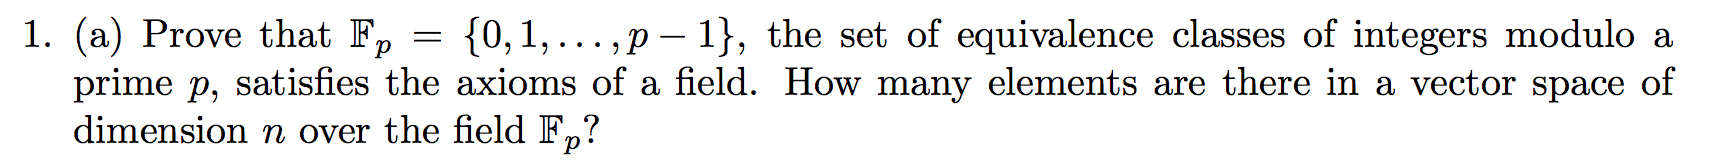
\includegraphics[width=450pt]{img/linear-algebra-a0-1-1-a.png}\\
\end{mdframed}

Let\footnote{Unlike the question, I am trying to use notation that
  distinguishes between integers and their equivalence classes.}
$a, b, c \in \Z$ with $0 \leq a < p, ~~ 0 \leq b < p, ~~ 0 \leq c < p$.

Let $\bar a, \bar b, \bar c \in \F$ be equivalence classes of integers modulo $p$.

The field axioms are listed below, together with proof that they hold for $\F_p$.
\begin{enumerate}
\item \textbf{$\F_p$ is an abelian group under addition}\\
  Define $\bar a + \bar b := \bar{a + b}$, then:
  \begin{enumerate}
  \item \textit{Existence of identity}: $\bar 0$ is the identity since
    $\bar a + \bar 0 = \bar{a + 0} = \bar{a}$ for all $\bar a \in \F_p$.
  \item \textit{Existence of inverses}: $(\bar a)^\1 = \bar{-a}$ since
    $\bar a + \bar{-a} = \bar{a + -a} = \bar{0}$ for all $a \in \F_p$.
  \item \textit{Commutativity}:
    $\bar a + \bar b = \bar{a + b} = \bar{b} + \bar{a}$ for all $a, b \in \F_p$.
  \item \textit{Associativity}:
    $\bar a + (\bar b + \bar c) = \bar a + \bar {b + c} = \bar{a + b + c} =
    \bar{a + b} + \bar{c} = (\bar a + \bar b) + \bar{c}$.
  \end{enumerate}
\item \textbf{$\F_p\setminus\{\bar 0\}$ is an abelian group under multiplication}\\
  Define $\bar a ~ \bar b := \bar{ab}$, then:
  \begin{enumerate}
  \item \textit{Existence of identity}: $\bar 1$ is the identity since
    $\bar a \bar 1 = \bar{a\cdot 1} = \bar{a}$ for all $\bar a \in \F_p$.
    \newpage
  \item \textit{Existence of inverses for everything except additive identity}:\\\\
    The claim is that for all $\bar a \in \F_p \setminus \{\bar 0\}$ there
    exists $\bar b \in \F_p$ such that $\bar a ~ \bar b = \bar 1$.

    \textbf{Proof 1}\\
    We show that elements cannot repeat in a row/column of the group operation
    table, therefore something muct be the inverse.
    \begin{align*}
      a \cdot b &= a \cdot c \mod p\\
      a(b - c) &= 0 \mod p\\
      a &= 0 \text{~or~~} b = c \mod p
    \end{align*}

    \textbf{Proof 2}\\
    Fix an arbitrary $a \in \{1, \ldots, p-1\}$.

    The claim is equivalent to the following: there exists
    $b \in \{0, 1, \ldots, p\}$ such that for all $i, j \in \Z$ there exists
    $k \in \Z$ such that $(ip + a)(jp + b) = kp + 1$.

    But note that $(ip + a)(jp + b) = p(ijp + aj + bi) + ab$ and therefore
    \begin{align*}
      &(ip + a)(jp + b) = kp + 1\\
      \iff &ab = p(k - ijp - aj - bi) + 1.
    \end{align*}
    Since $k$ can be chosen freely, the condition is simply that for all
    $i, j \in \Z$ there exists $k \in \Z$ such that $ab = kp + 1$.

    Note\footnote{I eventually allowed myself to google for a hint here which
      brought up people pointing to Bezout's identity.} that $a$ and $p$ are
    coprime (gcd is 1). By Bezout's identity, there exists $b, -k \in \Z$
    such that
    \begin{align*}
      ba + (-k)p = 1 \iff ab = kp + 1. \qed
    \end{align*}


  \item \textit{Commutativity}:
    $\bar a ~ \bar b = \bar{ab} = \bar{b} ~ \bar{a}$ for all $a, b \in \F_p$.
  \item \textit{Associativity}:
    $\bar a (\bar b \bar c) = \bar a + \bar {bc} = \bar{abc} =
    \bar{ab}~\bar{c} = (\bar a ~ \bar b) \bar{c}$.
  \end{enumerate}
\item \textbf{Distributive axiom}
  \begin{enumerate}
  \item \textit{Multiplication distributes over addition}: $\bar a (\bar b + \bar c) = \bar a (\bar{b + c}) = \bar{a(b+c)} = \bar{ab +
      ac} = \bar{ab} + \bar{ac} = \bar{a}~\bar{b} + \bar{a}~\bar{c}$
  \end{enumerate}
\end{enumerate}

There are $p^n$ elements in a vector space of dimension $n$ over the field $\F_p$.
\newpage
\begin{mdframed}
  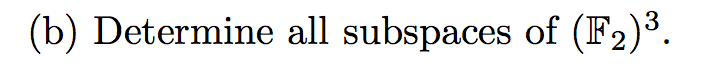
\includegraphics[width=200pt]{img/linear-algebra-a0-1-1-b.png}
\end{mdframed}

\textit{Remark}: This is like the 8 vectors that form the unit cube in
$\R^3$, except that when extended beyond the cube by vector addition or
scalar multiplication they ``wrap around''.

Note that
\begin{align*}
  (\F_2)^3 = \{&\bar 0, \bar 1\}^3\\
           = \{&(\bar 0, \bar 0, \bar 0),\\
               &(\bar 0, \bar 0, \bar 1),\\
               &(\bar 0, \bar 1, \bar 0),\\
               &(\bar 0, \bar 1, \bar 1),\\
               &(\bar 1, \bar 0, \bar 0),\\
               &(\bar 1, \bar 0, \bar 1),\\
               &(\bar 1, \bar 1, \bar 0),\\
               &(\bar 1, \bar 1, \bar 1)\}.
\end{align*}
The set of subspaces of $(\F_2)^3$ is
\begin{align*}
  &\{\{(\bar 0, \bar 0, \bar 0)\}\} ~~~~~~~~~~~~~~~~~~~~~ \cup\\
  &\{\{(\bar 0, \bar 0, \bar 0), x\} ~|~ x \in (\F_2)^3\} ~~~ \cup\\
  &\{\{(\bar 0, a, b) ~|~ a, b \in \F_2\}\}  ~~~~~~~ \cup\\
  &\{\{(a, \bar 0, b) ~|~ a, b \in \F_2\}\}  ~~~~~~~ \cup\\
  &\{\{(a, b, \bar 0) ~|~ a, b \in \F_2\}\}  ~~~~~~~ \cup\\
  &\{(\F_2)^3\}.
\end{align*}

\red{Per AC this is missing, at least, a subspace of size 4. Also see Sylov theorems.}

\newpage
\subsubsection{} % 2
\begin{mdframed}
  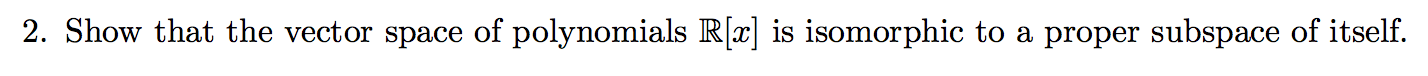
\includegraphics[width=450pt]{img/linear-algebra-a0-1-2.png}\\
\end{mdframed}
We need to:
\begin{enumerate}
\item \textbf{Exhibit a proper subspace $S[x] \subset \R[x]$ and a bijection $f:\R[x] \to S[x]$}\\\\
  Let $a_i \in \R$ for $i = 0, 1, 2, \ldots$ so that
  $\R[x] = \{a_0 + a_1x^1 + a_2x^2 + \ldots\}$.

  Define $S[x] = \{0 + a_1x^1 + a_2x^2 + a_3x^3 + \ldots\}$, i.e. the restriction
  of $\R[x]$ to those polynomials that have constant term zero.

  $S[x]$ is a proper subspace of $\R[x]$ since it contains the zero polynomial,
  and is closed under addition and scalar multiplication.

  Define $f: \R[x] \to S[x]$ where
  $f(a_0 + a_1x^1 + a_2x^2 + \ldots) = 0 + a_0x^1 + a_1x^2 + a_2x^3 + \ldots$.

  $f$ is clearly injective, since if $f(r(x)) = f(r'(x))$ then their
  coefficients $a_0, a_1, \ldots$ are the same and hence $r(x) = r'(x)$.

  Also, $f$ is clearly surjective since if
  $s(x) = a_1x^1 + a_2x^2 + a_3x^3 + \ldots$ then
  $s(x) = f(a_1 + a_2x^1 + a_3x^2 + \ldots)$.

\item \textbf{Prove that $f$ preserves addition}\\\\
  Let $a_i,b_i \in \R$ for $i = 0, 1, 2, \ldots$

  Let $r(x) = a_0 + a_1x^1 + a_2x^2 + \ldots$ and $r'(x) = b_0 + b_1x^1 + b_2x^2 + \ldots$.

  Then
  \begin{align*}
    f\Big(r(x) + r'(x)\Big)
    &= f\Big((a_0 + b_0) + (a_1 + b_1)x^1 + (a_2 + b_2)x^2 + \ldots\Big)\\
    &= 0 + (a_0 + b_0)x^1 + (a_1 + b_1)x^2 + (a_2 + b_2)x^3 + \ldots\\
    &= \Big(0 + a_0x^1 + a_1x^2 + a_2x^3 + \ldots \Big) \\
    &+ \Big(0 + b_0x^1 + b_1x^2 + b_2x^3 + \ldots \Big) \\
    &= f\Big(r(x)\Big) + f\Big(r'(x)\Big).
  \end{align*}

\item \textbf{Prove that $f$ preserves scalar multiplication}
  \begin{align*}
    f\Big(\lambda r(x)\Big)
    &= f\Big(\lambda a_0 + \lambda a_1x^1 + \lambda a_2x^2 + \ldots \Big) \\
    &= 0 + \lambda a_0x^1 + \lambda a_1x^2 + \lambda a_2x^3 + \ldots \\
    &= \lambda(0 + a_0x^1 + a_1x^2 + a_2x^3 + \ldots) \\
    &= \lambda f\Big(r(x)\Big)
  \end{align*}


\end{enumerate}

\newpage
\subsubsection{} % 3
\begin{mdframed}
  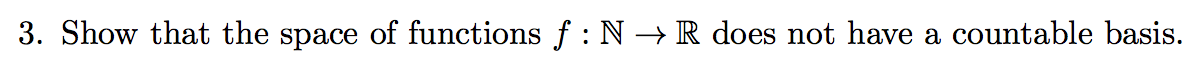
\includegraphics[width=400pt]{img/linear-algebra-a0-1-3.png}\\
\end{mdframed}

Note:
\begin{enumerate}
\item The space of functions $f:\N \to \R$ is the space of real-valued
  infinite sequences.
\item A basis is countable iff a bijection exists between the basis and $\N$.
\end{enumerate}

\red{I haven't managed to do this. What follows is what I was thinking, but
  must be wrong since it contradicts the question.}

Let $x_i \in \R$ for
$i \in \N$ and define the following:
\begin{itemize}
\item $F_n := \{(x_1, x_2, \ldots, x_n) ~|~ x_1, x_2, \ldots, x_n \in \R\}$ is
  the space of functions\\$f:\{1,2, \ldots, n\} \to \R$
\item $F_\infty := \{(x_1, x_2, \ldots) ~|~ x_1, x_2, \ldots \in \R\}$ is the
  space of functions $f:\N \to \R$.
\end{itemize}

Note that $F_1 = \{x_1 ~|~ x_1 \in \R\} = \R$. Therefore every basis for $F_1$ has cardinality
1 (every basis is a set containing a single non-zero real number).

Similarly, $F_2 = \R^2$, and every basis of $F_2$ has cardinality 2.

\red{Basically it seems like the following is a basis of this space of functions,
  but it is countable:}
\begin{align*}
  &(1, 0, 0, \ldots),\\
  &(0, 1, 0, \ldots),\\
  &(0, 0, 1, \ldots),\\
  &\ldots\\
\end{align*}

\red{I think the answer here is that $E$ is a basis for $F_\infty$ iff every
  element of $F_\infty$ can be expressed as a linear combination of a
  \textit{finite} number of elements from $E$. But this is untrue, at least for
  the basis I have suggested, since for example the constant function
  $f(i) = 1 ~\forall i$ fails.}

% ~\\
% \hrule




\newpage
\subsubsection{} % 4
\begin{mdframed}
  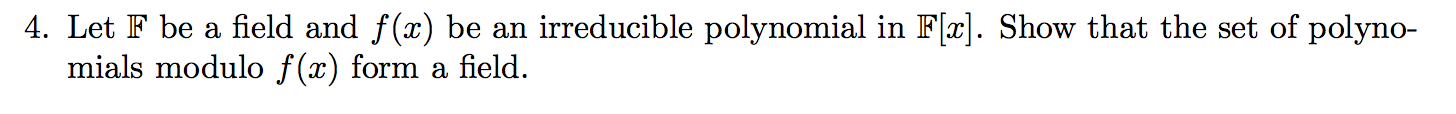
\includegraphics[width=400pt]{img/linear-algebra-a0-1-4.png}\\
\end{mdframed}
Let $P$ be the set of polynomials modulo $f(x)$.

The field axioms are listed below, together with proof that they hold for $P$.
\begin{enumerate}
\item \textbf{$P$ is an abelian group under addition}\\\\
  Define $\bar{g(x)} + \bar{h(x)} := \bar{g(x) + h(x)}$, then:
  \begin{enumerate}
  \item \textit{Existence of identity}:\\
    The additive identity is $\bar 0 = \Big\{f(x)g(x) ~|~ g(x) \in \F[x]\Big\}$.

  \item \textit{Existence of inverses}:\\
    $\bar{g(x)}^{~\1} = \bar{-g(x)}$ for all $g(x) \in P$.
  \item \textit{Commutativity and Associativity}:\\
    Proofs of these are essentially the same as for $\F_p$ (question 1).
  \end{enumerate}
\item \textbf{$P\setminus\{\bar 0\}$ is an abelian group under multiplication}\\\\
  Define $\bar{g(x)} \cdot \bar{h(x)} := \bar{g(x)\cdot h(x)}$, then:
  \begin{enumerate}
  \item \textit{Existence of identity}:\\
    The multiplicative identity is $\bar 1 = \Big\{f(x)g(x) + 1~|~ g(x) \in \F[x]\Big\}$.

  \item \textit{Existence of inverses for everything except additive identity}:\\\\
    The claim is that for all $\bar a \in \F_p \setminus \{\bar 0\}$ there
    exists $\bar b \in \F_p$ such that $\bar a ~ \bar b = \bar 1$.

    Fix an arbitrary $a \in \{1, \ldots, p-1\}$.

    The claim is equivalent to the following: there exists
    $b \in \{0, 1, \ldots, p\}$ such that for all $i, j \in \Z$ there exists
    $k \in \Z$ such that $(ip + a)(jp + b) = kp + 1$.

    But note that $(ip + a)(jp + b) = p(ijp + aj + bi) + ab$ and therefore
    \begin{align*}
      &(ip + a)(jp + b) = kp + 1\\
      \iff &ab = p(k - ijp - aj - bi) + 1.
    \end{align*}
    Since $k$ can be chosen freely, the condition is simply that for all
    $i, j \in \Z$ there exists $k \in \Z$ such that $ab = kp + 1$.

    Note\footnote{I eventually allowed myself to google for a hint here which
      brought up people pointing to Bezout's identity.} that $a$ and $p$ are
    coprime (gcd is 1). By Bezout's identity, there exists $b, -k \in \Z$
    such that
    \begin{align*}
      ba + (-k)p = 1 \iff ab = kp + 1. \qed
    \end{align*}


  \item \textit{Commutativity}:
    $\bar a ~ \bar b = \bar{ab} = \bar{b} ~ \bar{a}$ for all $a, b \in \F_p$.
  \item \textit{Associativity}:
    $\bar a (\bar b \bar c) = \bar a + \bar {bc} = \bar{abc} =
    \bar{ab}~\bar{c} = (\bar a ~ \bar b) \bar{c}$.
  \end{enumerate}
\item \textbf{Distributive axiom}
  \begin{enumerate}
  \item \textit{Multiplication distributes over addition}: $\bar a (\bar b + \bar c) = \bar a (\bar{b + c}) = \bar{a(b+c)} = \bar{ab +
      ac} = \bar{ab} + \bar{ac} = \bar{a}~\bar{b} + \bar{a}~\bar{c}$
  \end{enumerate}
\end{enumerate}

\newpage

\begin{mdframed}
  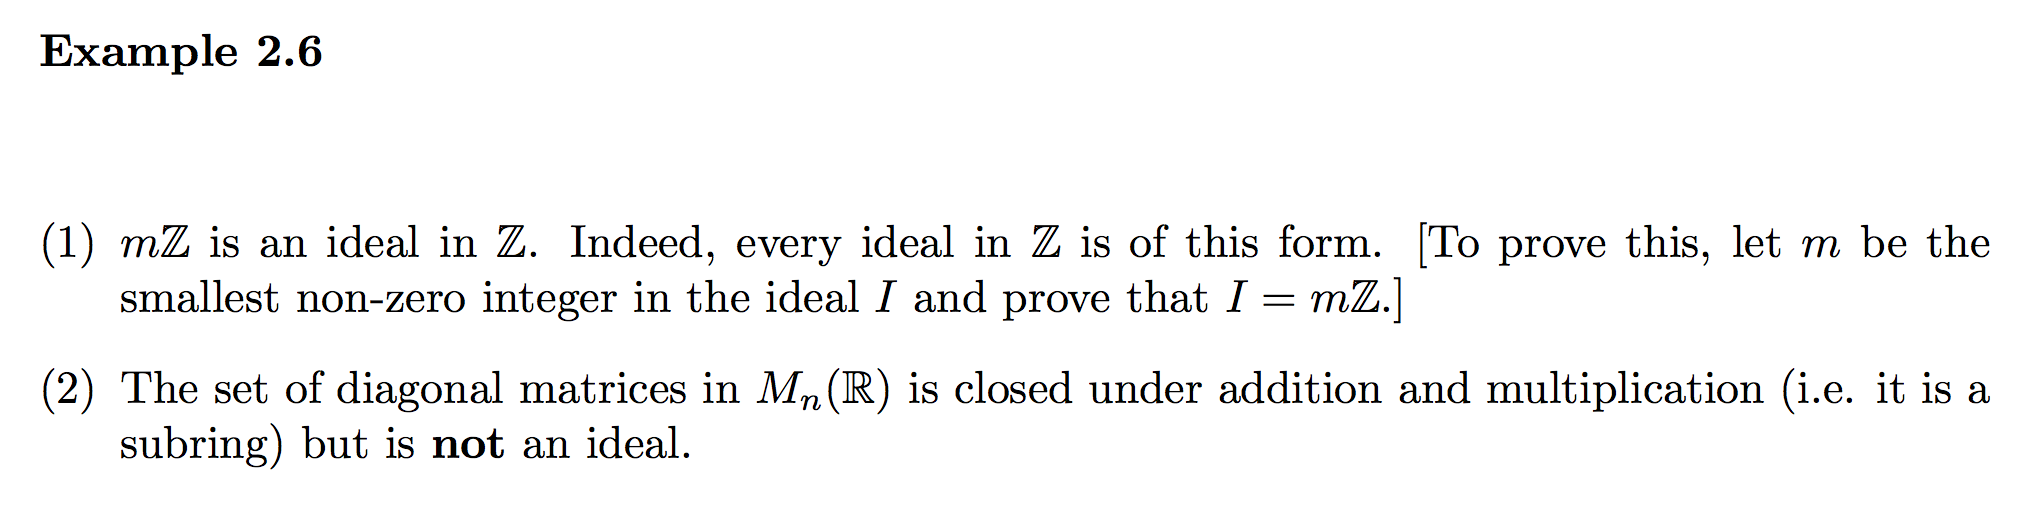
\includegraphics[width=400pt]{img/linear-algebra-eg-2-6.png}
\end{mdframed}

\begin{claim*}
  $m\Z$ is an ideal in $\Z$.
\end{claim*}

\begin{proof}Let $s, t \in m\Z$ and $i, j, k \in \Z$.

  Then $s = mi$ and $t = mj$ for some $i, j$.

  Therefore $s - t = m(i - j) \in m\Z$ and $ks = sk = m(ki) \in m\Z$.
\end{proof}

\begin{claim*}
  Every ideal in $\Z$ is of the form $m\Z$.
\end{claim*}

\begin{proof}
  Let $I$ be an ideal in $\Z$ and let $m$ be the smallest non-zero positive integer in $I$.

  % Let $i \in I$. We have that $i - m \in I$ and that $mi \in I$.

  % We want to show that $i \in m\Z$.

  Let $i \in I$. We want to show that $i \in m\Z$.

  We have:

  $ki \in I$ for all $k \in \Z$.

  $i - j \in I$ for all $j \in I$.

  $i - m \in I$.


  % By the definition of an ideal, $ki \in I$ for
  % all $k \in \Z$. Therefore $i$ is a multiple of $m$.

  % Conversely, suppose $i \in m\Z$. We want to show that $i \in I$.


  % is a multiple of $m$. So $i = km$ for some $k \in \Z$.
\end{proof}


\newpage
\subsubsection{} % 5
\begin{mdframed}
  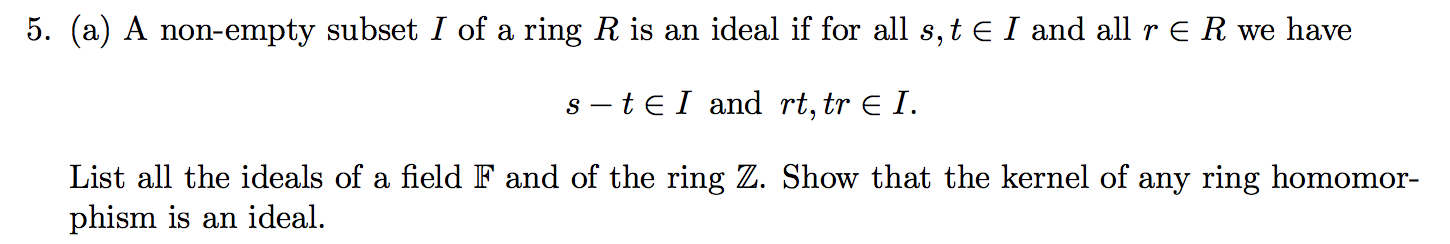
\includegraphics[width=400pt]{img/linear-algebra-a0-1-5-a.png}\\
\end{mdframed}

The set of ideals of a field $\F$ is $\{a\F ~|~ a \in \F\} = \{\{0\}, \F\}$.

The set of ideals of the ring $\Z$ is $\{m\Z ~|~ m \in \Z\}$.


\begin{definition*}
  Let $R, S$ be rings and let $r_1, r_2 \in R$. A \emph{ring homomorphism} is $f:R \to S$ such that
  $f(r_1 + r_2) = f(r_1) + f(r_2)$ and $f(r_1r_2) = f(r_1)f(r_2)$.
\end{definition*}

\begin{claim*}
  The kernel of any ring homomorphism is an ideal.
\end{claim*}

\begin{proof}
  Let $H$ be the kernel of a ring homomorphism $f:R \to S$, and let

  We want to show that
  \begin{enumerate}
  \item $h_1 - h_2 \in H$ for all $h_1, h_2 \in H$, and \label{ring-hom-ideal-1}
  \item $rh \in H$ for all $r \in R, h \in H$. \label{ring-hom-ideal-2}
  \end{enumerate}

  We have $f(h_1 - h_2) = f(h_1) + f(-h_2) = f(h_1) - f(h_2) = 0 - 0 = 0$, proving
  (\ref{ring-hom-ideal-1}).

  And $f(rh) = f(r)f(h) = f(r)\cdot 0 = 0$, proving (\ref{ring-hom-ideal-2}).

\end{proof}



\newpage
\begin{mdframed}
  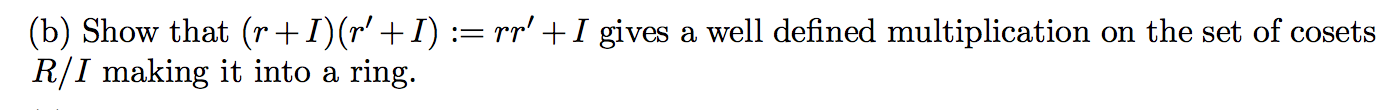
\includegraphics[width=400pt]{img/linear-algebra-a0-1-5-b.png}\\
\end{mdframed}

\begin{mdframed}
  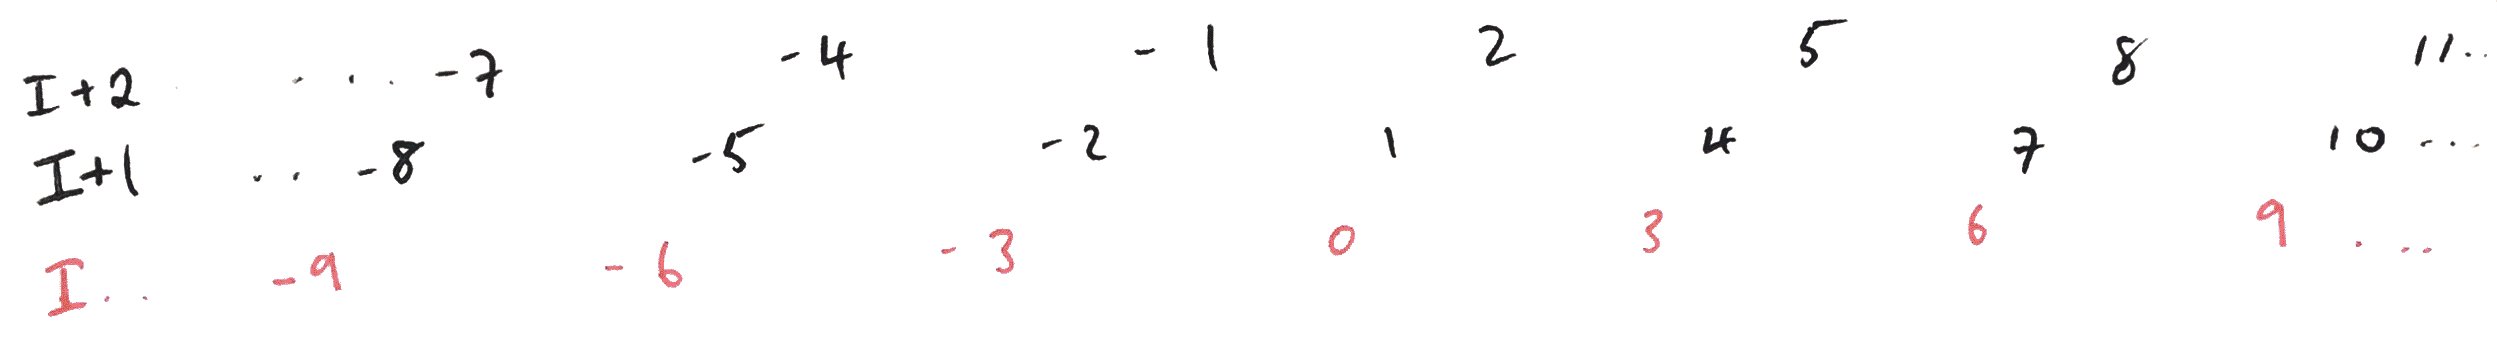
\includegraphics[width=400pt]{img/ideal-in-integers.png}
\end{mdframed}

\begin{mdframed}
  \begin{remark*}
    Recall that in group theory a quotient group is formed by:
    \begin{enumerate}
    \item Identify a subgroup.
    \item Form cosets.
    \item Inherit operation on cosets from operation on original group elements.
    \end{enumerate}
    But only if the subgroup is normal.

    Here, the ideal $I$ is playing the role of subgroup.~\\
  \end{remark*}
\end{mdframed}

Let $S$ and $T$ be cosets, and let $r \in S$ and $r' \in T$. We need to show that $rr' + I$ is the
same coset, for all choices of $r$, $r'$.

\newpage
\begin{mdframed}
  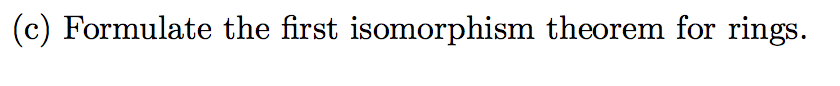
\includegraphics[width=280pt]{img/linear-algebra-a0-1-5-c.png}\\
\end{mdframed}

\newpage
\subsubsection{} % 6
\begin{mdframed}
  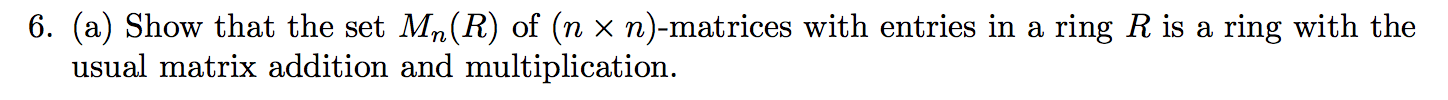
\includegraphics[width=400pt]{img/linear-algebra-a0-1-6-a.png}\\
\end{mdframed}
It is an abelian group under addition since:
\begin{enumerate}
\item The zero matrix is the additive identity.
\item For all $r \in R$, we have $-r \in R$. Therefore for $A \in M_n(R)$ we have $-A \in M_n(R)$.
\item It is closed (result is a matrix of same dimension).
\item Addition commutes.
\end{enumerate}

Under multiplication:
\begin{enumerate}
\item It is closed because addition and multiplication in the ring are closed.
\item Multiplication is associative.
\item Both distributive laws hold ($A(B + C) = AB + AC$ and $(B + C)A = BA + CA$.)
\end{enumerate}

Therefore it is a ring (but not a field since multiplicative inverses may not exist).

\begin{mdframed}
  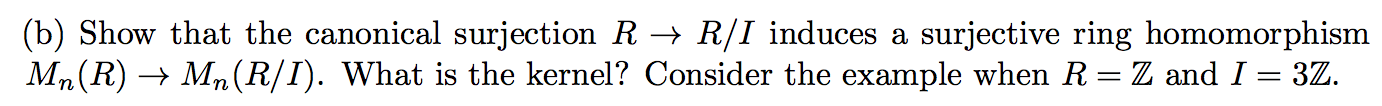
\includegraphics[width=400pt]{img/linear-algebra-a0-1-6-b.png}\\
\end{mdframed}
Let $I$ be an ideal of a ring $R$.

Note that:
\begin{enumerate}
\item If $r$ is an entry in a matrix $A \in M_n(R)$ then $r \in R$.
\item If $s$ is an entry in a matrix $\Gamma \in M_n(R/I)$ then $s \in R/I$ is a coset.
\end{enumerate}

The ``canonical surjection'' $R \to R/I$ is defined by $r \mapsto rI$.

It induces a map $f:M_n(R) \to M_n(R/I)$ defined by $A \mapsto \Gamma$, where
$\Gamma_{ij} = A_{ij}I$ for all $i,j \in \{1, \ldots, n\}$.

Let $A, B \in M_n(R)$.

Then
\begin{align*}
  \Big(f(A + B)\Big)_{ij}
  &= (A_{ij} + B_{ij})I ~~~~~~~~~~~~~~~~~~~\text{(by definition of the induced map)}\\
  &= A_{ij}I + B_{ij}I ~~~~~~~~~~~~~~~~~~~~\text{(by definition of addition on the cosets)}\\
  &= \Big(f(A)\Big)_{ij} + \Big(f(B)\Big)_{ij} ~~~~~~~\text{(by definition of the induced map)}\\
  &= \Big(f(A) + f(B)\Big)_{ij}~~~~~~~~~~~~~\text{(by definition of matrix addition)},\\
\end{align*}

and

\begin{align*}
  \Big(f(AB)\Big)_{ij}
  &= (AB)_{ij}I ~~~~~~~~~~~~~~~~~~~\text{(by definition of the induced map)}\\
  &= \sum_k A_{ik}B_{kj}I\\
  &= \sum_k (A_{ik}I)(B_{kj}I)\\
  &= \Big(f(A)f(B)\Big)_{ij}.
\end{align*}

Therefore $f$ preserves the additive and multiplicative structure on $M_n(R)$.

\red{TODO: show it is surjective}

The additive identity in $M_n(R/I)$ is the matrix containing $I$ in every entry.

The kernel is the set of matrices that get mapped to the (additive) identity in $M_n(R/I)$.

Therefore the kernel is $\{A ~|~ A_{ij} \in I ~\forall~ i, j \in \{1, \ldots, n\}\}$.

For example, suppose $R = \Z$ and $I = 3\Z$.

Then $R/I = \{3\Z, 3\Z + 1, 3\Z + 2\}$.

The kernel is $\{A ~|~ A_{ij} \in 3\Z\}$.

\begin{mdframed}
  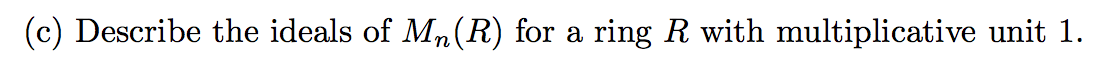
\includegraphics[width=350pt]{img/linear-algebra-a0-1-6-c.png}\\
\end{mdframed}
The set of diagonal matrices is the sole ideal?

\newpage
\subsubsection{} % 7
\begin{mdframed}
  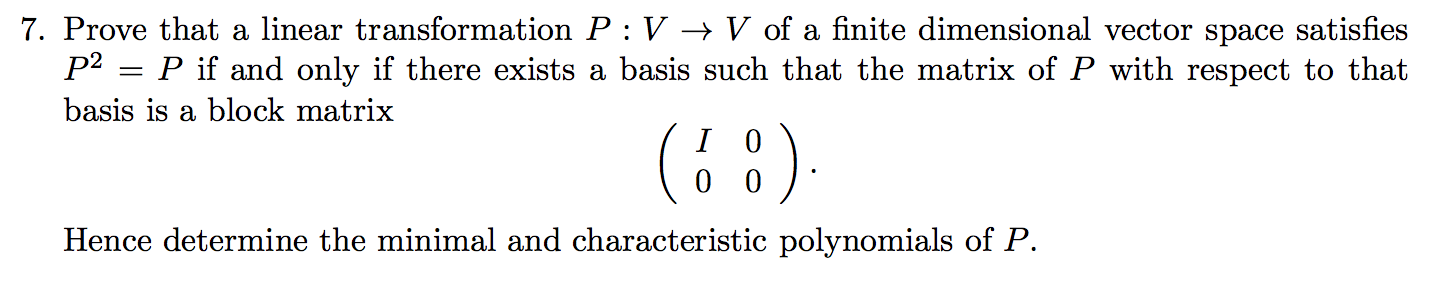
\includegraphics[width=400pt]{img/linear-algebra-a0-1-7.png}\\
\end{mdframed}

\subsubsection{} % 8
\begin{mdframed}
  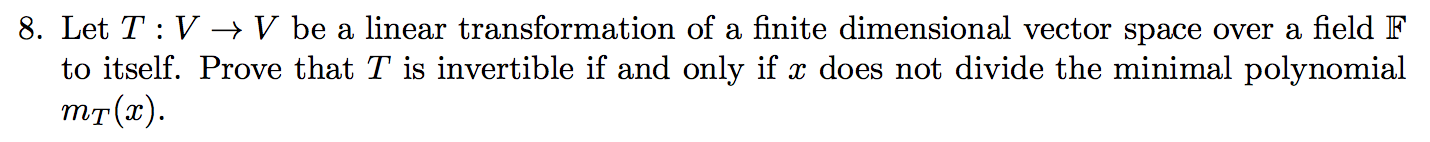
\includegraphics[width=400pt]{img/linear-algebra-a0-1-8.png}\\
\end{mdframed}

\subsubsection{} % 9
\begin{mdframed}
  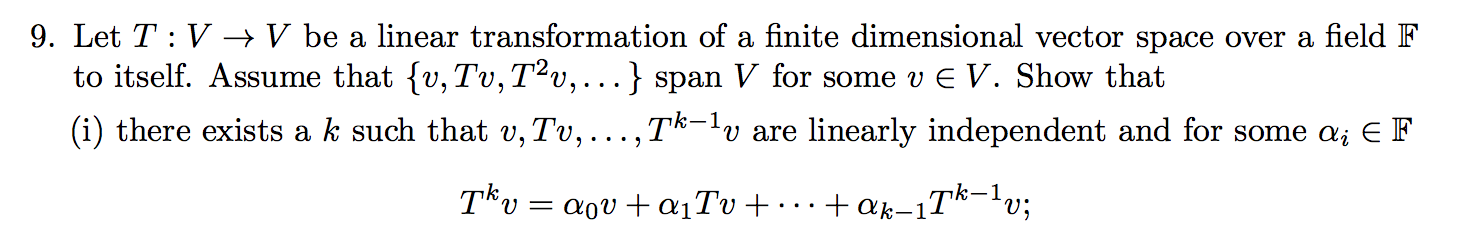
\includegraphics[width=400pt]{img/linear-algebra-a0-1-9-a.png}\\
\end{mdframed}
\begin{mdframed}
  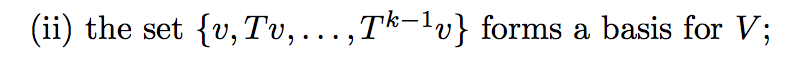
\includegraphics[width=250pt]{img/linear-algebra-a0-1-9-b.png}\\
\end{mdframed}
\begin{mdframed}
  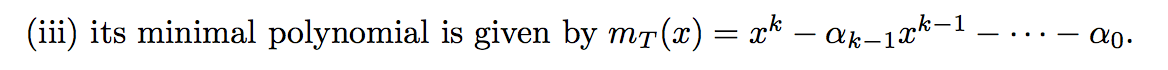
\includegraphics[width=350pt]{img/linear-algebra-a0-1-9-c.png}\\
\end{mdframed}
\begin{mdframed}
  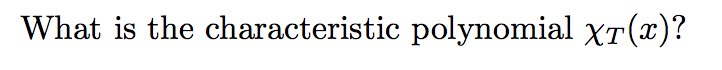
\includegraphics[width=220pt]{img/linear-algebra-a0-1-9-d.png}\\
\end{mdframed}

\newpage
\subsection{Sheet 2}

% https://math.stackexchange.com/questions/555726/inducing-a-linear-map-on-quotient-spaces
\begin{mdframed}
  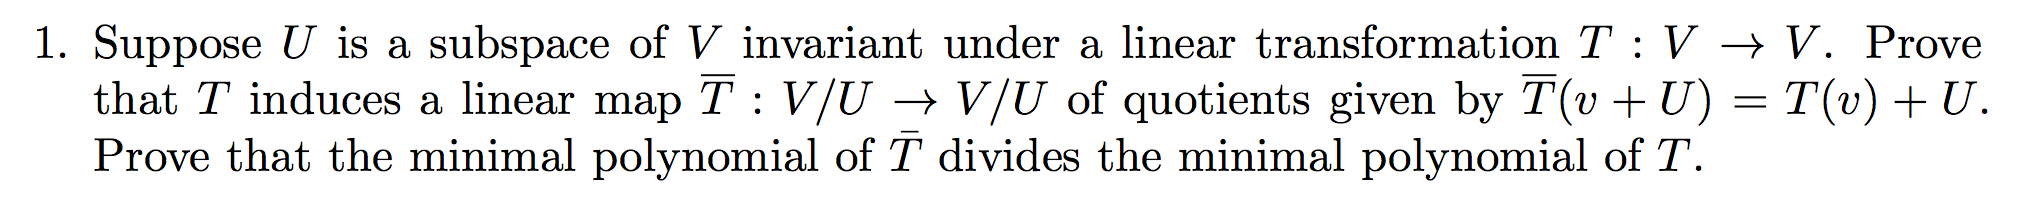
\includegraphics[width=400pt]{img/linear-algebra-a0-2-1.png}
\end{mdframed}
\begin{mdframed}
  \begin{example*}
    Let $V = \R^3$, $U$ be a one-dimensional subspace, and $T$ be rotation around the axis
    $U$. Choose an orthonormal basis $\{w, v, u\}$ for $\R^3$ where $u \in U$. Then the matrix
    of $T$ is
    \begin{align*}
      \matMMMxNNN
      {\cos\theta}{-\sin\theta}{0}
      {\sin\theta}{~~\cos\theta}{0}
      {0}         {           0}{1}.
    \end{align*}

    $V/U$ is the set of lines parallel to $U$. $U$ is the kernel of a projection onto $\R^2$, and
    $V/U \cong \R^2$.

    ``In some sense'' the matrix of $\bar T:V/U \to V/U$ is the block
    $\matMMxNN{\cos\theta}{-\sin\theta}
    {\sin\theta}{~~\cos\theta}$.
  \end{example*}
\end{mdframed}

Let $v + U$ be a coset of $U$. Then the induced mapping is given by
\begin{align*}
  \bar T(v + U) &= \{T(v + u) ~|~ u \in U\}\\
                &= \{T(v) + T(u) ~|~ u \in U\}\\
                &= T(v) + T(U)\\
                &= T(v) + U.
\end{align*}

\begin{claim*}
  $\bar T$ is a linear map.
\end{claim*}

\begin{proof}~\\
  \red{TODO: is there any question about it being well-defined?}

  Vector addition:
  \begin{align*}
    \bar T\Big((v + U) + (w + U)\Big)
    &= \bar T\Big((v + w) +  U\Big) ~~~~~~~~~~~~~\text{(by definition of addition on quotient group)}\\
    &= T(v + w) + U              ~~~~~~~~~~~~~~~~~\text{(by definition of $\bar T$)}\\
    &= (T(v) + T(w)) + U              ~~~~~~~~~~\text{(by linearity of $T$)}\\
    &= (T(v) + U) + (T(w) + U) ~~\text{(by definition of addition on quotient group)}\\
    &= \bar T(v + U) + \bar T(w + U)              ~~~~~~~\text{(by definition of $\bar T$)}
  \end{align*}
  Multiplication by a scalar $\lambda \in \F$:
  \begin{align*}
    \bar T\Big(\lambda(v + U)\Big)
    &= \bar T\Big(\lambda v + \lambda U\Big) ~~\text{(by (scalar)(SetOfVectors) and (vector) + (SetOfVectors) syntax)}\\
    &= T(\lambda v) + \lambda U~~~~\text{(by definition of $\bar T$)}\\
    &= \lambda T(v) + \lambda U~~~~\text{(by linearity of $T$)}\\
    &= \lambda\Big(T(v) + U\Big)  ~~\text{(by (scalar)(SetOfVectors) and (vector) + (SetOfVectors) syntax)}\\
    &= \lambda \bar T(v + U)~~~~~\text{(by definition of $\bar T$)}
  \end{align*}
\end{proof}

\begin{definition*}[Minimal polynomial]
  Let $V$ be a finite-dimensional vector space over $\F$, and let $A$ be a matrix of a linear
  transformation $T:V \to V$.

  The \emph{minimal polynomial} $m_A(x)$ is the monic polynomial $p(x)$ of minimal degree such that
  $p(A) = 0$.
\end{definition*}

\begin{lemma*}~\\
  \begin{enumerate}
  \item The minimal polynomial exists for any endomorphic linear transformation.
  \item The minimal polynomial is unique.
  \item Let $f(x)$ be a polynomial. If $f(A) = 0$ then $m_A | f$.
  \end{enumerate}
\end{lemma*}

\begin{claim*}
  The minimal polynomial of $\bar T$ divides the minimal polynomial of $T$.
\end{claim*}

\begin{proof} (I)\\

  \begin{align*}
    m_T(\bar T)
  \end{align*}

  $\vdots$

  We have $m_T(\bar T) = 0$, therefore $m_{\bar T}| m_T$.

\end{proof}

\begin{proof} (II)\\
  Let $J = \dim U$ and $K = \dim V$.

  Pick a basis of $U$ and extend it to a basis $\mathcal B$ of $V$.

  Order the elements of the basis $\mathcal B$ such that the last $J$ elements are the basis of
  $U$.

  Let $A$ be the matrix of $T$ with respect to $\mathcal B$.

  Then, since $U$ is invariant under $T$, $A$ has a block structure
  \begin{align*}
    A = \matMMxNN{~\bar A}{0}
                 {~0     }{B}.
  \end{align*}

  Claim: $\bar A$ is the matrix of $\bar T$ with respect to some basis of $V/U$.

  Note that
  \begin{align*}
    \lambda A^n = \matMMxNN{~\lambda{\bar A}^n}{0}
                            {~0      }{\lambda B^n}.
  \end{align*}
  Let $p(x)$ be a polynomial. Then $p(A) = 0 \implies p(\bar A) = 0$.

  Let $m_A(x)$ and $m_{\bar A}(x)$ be the minimal polynomials of $A$ and $\bar A$ respectively.

  By definition, $m_A(A) = 0$.

  Therefore $m_A(\bar A) = 0$, therefore $m_{\bar A}| m_A$.

  Equivalently, $m_{\bar T}| m_T$.
\end{proof}


% \newpage
\begin{mdframed}
  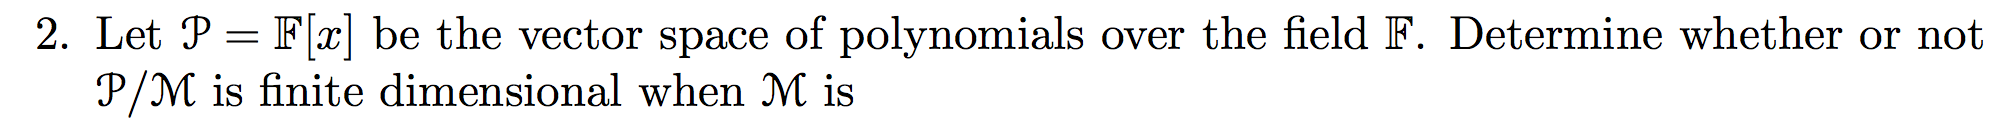
\includegraphics[width=400pt]{img/linear-algebra-a0-2-2.png}
\end{mdframed}
\begin{mdframed}
  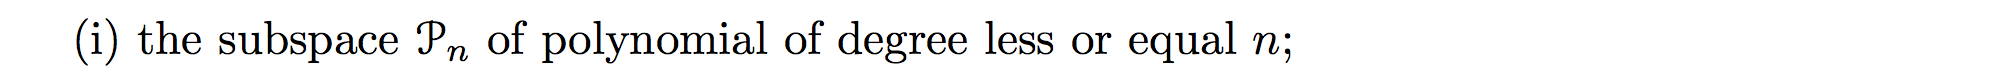
\includegraphics[width=400pt]{img/linear-algebra-a0-2-2-1.png}
\end{mdframed}

Let $D^n:\mc P \to \mc P$ be the $n$-th derivative operator.

Then $\mc P_n$ is the kernel of $D^{n+1}$.

Furthermore, $D^n$ is a homomorphism (preserves addition of polynomials).

By the First Isomorphism Theorem, $\mc P/\mc P_n \cong \Im D^{n+1}$.

\begin{claim*}
  $\Im D^n = \mc P$ (surjective) for all $n \in \N$.
\end{claim*}

\begin{proof}
  Let $p(x) = \sum_{i=1}^k\lambda_ix^i \in \mc P$. Then
  $D^n \Big(x^n\sum_{i=1}^k\frac{\lambda_i}{(i>+n)_{(n)}}x^i\Big) = p(x)$, so $D^n$ is surjective.
\end{proof}

Therefore $\mc P/\mc P_n \cong \mc P$.

Therefore $\mc P/\mc P_n$ is infinite-dimensional.

\begin{remark*}
  Each element of $\mc P/\mc P_n$ is a set of polynomials differing only by additive terms
  of degree $n$ or less.
\end{remark*}

\begin{mdframed}
  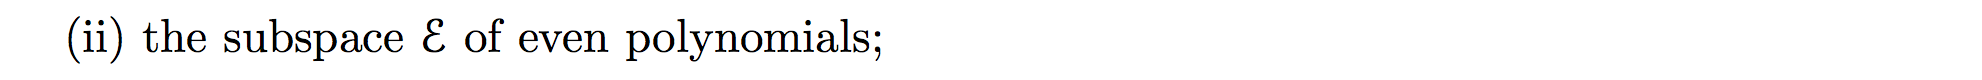
\includegraphics[width=400pt]{img/linear-algebra-a0-2-2-2.png}
\end{mdframed}
Let $\mc E$ and $\mc O$ be the set of even and odd polynomials respectively.

Let $f:\mc P \to \mc P$ be given by $p(x) := $ (the odd terms of $p(x)$).

Then $\Im f = \mc O$ and $\Ker f = \mc E$.

Therefore $\mc P/\mc E \cong \mc O$, infinite-dimensional.


\begin{mdframed}
  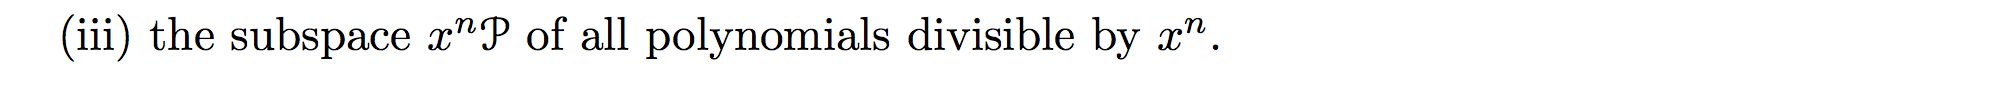
\includegraphics[width=400pt]{img/linear-algebra-a0-2-2-3.png}
\end{mdframed}
Let $f: \mc P \to \mc P$ be given by $f(p(x)) := $ (remainder after division by $x^n$).

\begin{claim*}
  $f$ is a homomorphism: $f(p(x) + q(x)) = f(p(x)) + f(q(x))$.
\end{claim*}

Note that $x^n\mc P$ is the kernel of $f$.

\begin{claim*}
  $\Im f = \mc P_{n-1}$.
\end{claim*}

\red{TODO: prove or disprove}.

If these claims are true, then $\mc P/x^n\mc P \cong \mc P_n$, finite-dimensional.

\begin{mdframed}
  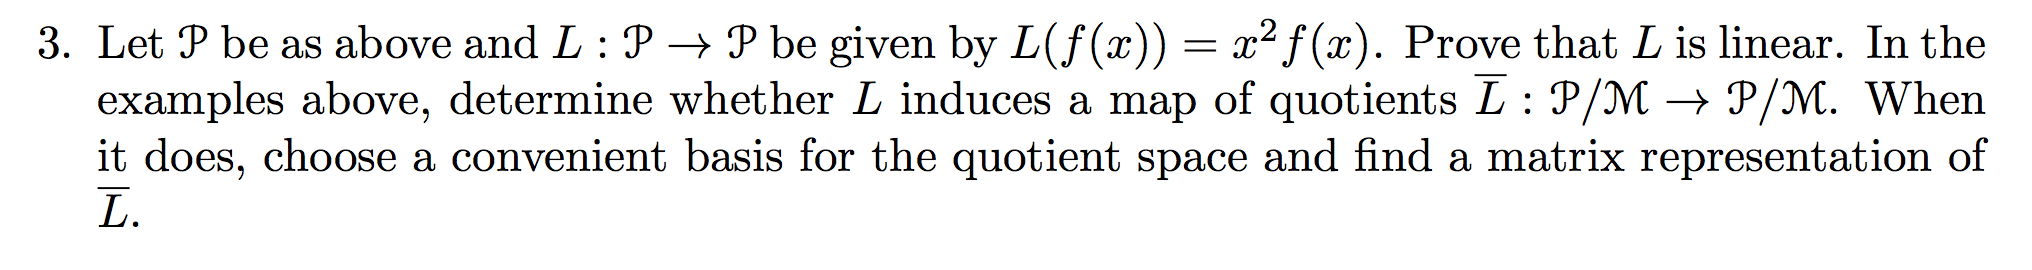
\includegraphics[width=400pt]{img/linear-algebra-a0-2-3.png}
\end{mdframed}

\begin{claim*}
  $L$ is linear.
\end{claim*}

\begin{proof} Note that multiplication of polynomials distributes over addition:
  \begin{align*}
    \Big(\sum_{i=0}^k a_ix^i\Big)\Big(\sum_{i=0}^k b_ix^i + \sum_{i=0}^k c_ix^i\Big)
    &= \Big(\sum_{i=0}^k a_ix^i\Big)\Big(\sum_{i=0}^k (b_i + c_i)x^i\Big)\\
    &= \Big(\sum_{i=0}^{k}\sum_{j=0}^k a_i(b_j + c_j)x^{i+j}\Big)\\
    &= \Big(\sum_{i=0}^{k}\sum_{j=0}^k a_ib_jx^{i+j}\Big) +
       \Big(\sum_{i=0}^{k}\sum_{j=0}^k a_ic_jx^{i+j}\Big)\\
    &= \Big(\sum_{i=0}^k a_ix^i\Big)\Big(\sum_{i=0}^k b_ix^i\Big) +
       \Big(\sum_{i=0}^k a_ix^i\Big)\Big(\sum_{i=0}^k c_ix^i\Big).
  \end{align*}
  Therefore
  \begin{align*}
    L(af(x) + bg(x)) &= x^2(af(x) + bg(x))\\
                     &= ax^2f(x) + bx^2g(x)\\
                     &= aL(f(x)) + bL(g(x)),
  \end{align*}
  where $a, b \in \F$.
\end{proof}

\newpage
\begin{mdframed}
  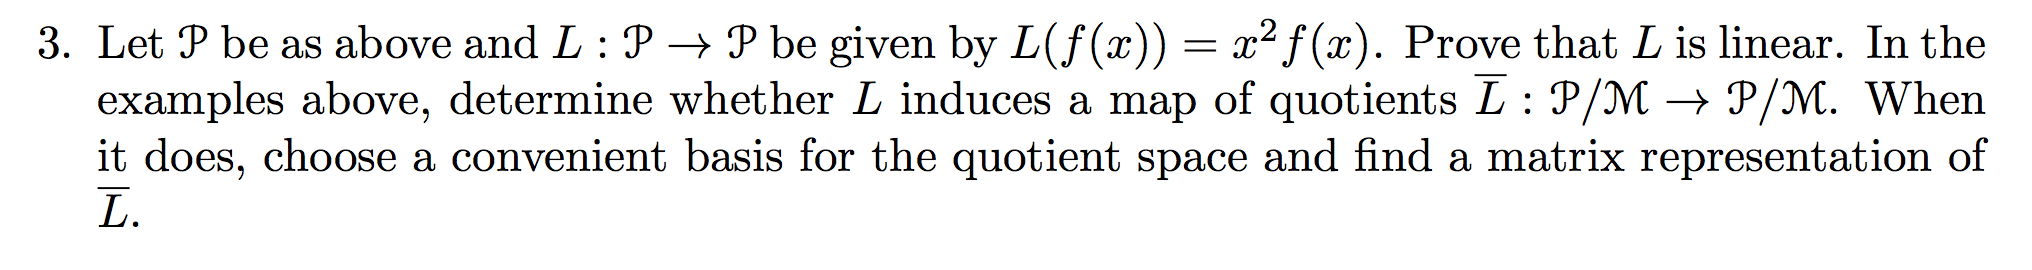
\includegraphics[width=400pt]{img/linear-algebra-a0-2-3.png}
\end{mdframed}

First, a theorem and a corollary:

\begin{theorem*}
  Let $L:V \to W$ be an isomorphism\footnote{note: not linear; but why not homomorphism?} between
  vector spaces $V$ and $W$, and let $A \subseteq V, B \subseteq W$ be subspaces. Then the formula
  $\bar L(v + A) = L(v) + B$ gives a well-defined linear map $\bar L:V/A \to W/B$ if and only if
  $L(A) \subseteq B$.
\end{theorem*}

Therefore

\begin{corollary*}
  Let $L:V \to V$ with $U$ a subspace of $V$. Then $L$ induces a linear map of quotients
  $\bar L:V/U \to V/U$ given by $v + U \mapsto L(v) + U$ if and only if $U$ is invariant under $T$.
\end{corollary*}

~\\

\begin{mdframed}
  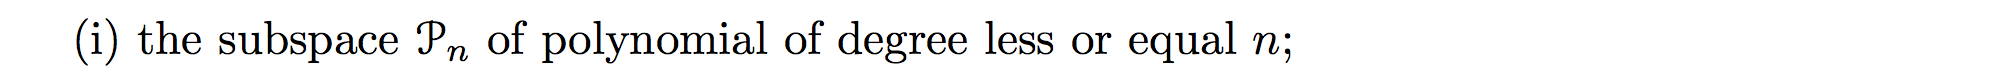
\includegraphics[width=400pt]{img/linear-algebra-a0-2-2-1.png}
\end{mdframed}

% Recall that:
% \begin{enumerate}
% \item $\mc P_n$ is the kernel of $D^{(n+1)}$.
% \item Every coset $\Big(p(x) + \mc P_n\Big) \in \mc P/\mc P_n$ is a set of polynomials differing
%   only by additive terms of degree $n$ or less.
% \end{enumerate}

Note that $L(\mc P_n) = x^2\mc P_n = \mc P_{n+2} \not\subseteq \mc P_n$.

Therefore the formula
\begin{align*}
  \bar L\Big(p(x) + \mc P_n\Big) := x^2p(x) + \mc P_n
\end{align*}
does not give a well-defined map $\bar L:\mc P/\mc P_n \to \mc P/\mc P_n$.

\begin{mdframed}
  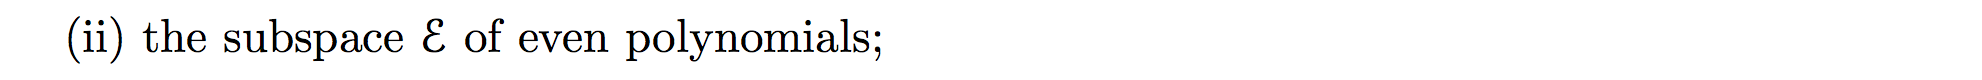
\includegraphics[width=400pt]{img/linear-algebra-a0-2-2-2.png}
\end{mdframed}

% Recall that:
% \begin{enumerate}
% \item $\mc P/\mc E \cong \mc O$, infinite-dimensional.
% \item Every coset is of the form $o(x) + \mc E$, for some odd polynomial $o(x) \in \mc O$.
% \end{enumerate}

Note that $L(\mc E) = x^2\mc E = \mc E$. Therefore the formula
\begin{align*}
  \bar L\Big(p(x) + \mc E\Big) := x^2p(x) + \mc E
\end{align*}
does give a well-defined linear map of quotients $\bar L:\mc P/\mc E \to \mc P/\mc E$.

A basis for $\mc E$ is $\{1, x^2, x^4, \ldots\}$.

To extend this basis to a basis for $\mc P$ we can add the elements of $\{x, x^3, x^5, \ldots\}$.

Therefore (theorem) a basis for $\mc P/\mc E$ is $\{x + \mc E, x^3 + \mc E, x^5 + \mc E, \ldots\}$.

However, the quotient space $\mc P/\mc E \cong \mc O$ is infinite-dimensional and therefore
$\bar L$ has no matrix representation.

% \begin{mdframed}
%   \begin{remark*}
%     Note that $\mc E$ is not in the basis since it is the additive identity in $\mc P/\mc E$: Let 0
%     be the additive identity in the field $\F$. Then
%     $\mc E = 0(x + \mc E) + 0(x^3 + \mc E) + \ldots$. This is true since in general
%     $0\vec v = (1 - 1)\vec v = \vec v - \vec v = \vec 0$.
%   \end{remark*}
% \end{mdframed}

% Since the quotient space is infinite-dimensional, $\bar L$ has no finite matrix representation.

% As an ``infinite matrix'' it would be
% \begin{align*}
%   \begin{pmatrix}
%     0      & 0      & 0      & \cdots\\
%     1      & 0      & 0      & \cdots\\
%     0      & 1      & 0      & \cdots\\
%     \vdots & \vdots & \vdots & \ddots
%   \end{pmatrix},
% \end{align*}
% that is, an infinite-dimensional identity matrix below a row of zeros.

\begin{mdframed}
  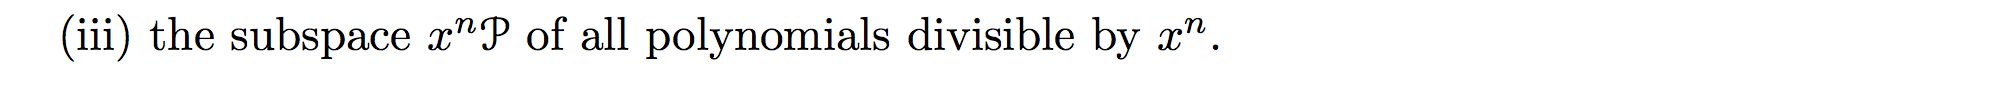
\includegraphics[width=400pt]{img/linear-algebra-a0-2-2-3.png}
\end{mdframed}

% Recall that:
% \begin{enumerate}
% \item $x^n\mc P$ is the kernel of the homomorphism which sends $p(x) \in \mc P$ to its remainder
%   after division by $x^n$. The image is $\mc P_{n-1}$.
% \item Therefore $\mc P/x^n\mc P \cong \mc P_{n-1}$, finite-dimensional.
% \item Every coset is of the form $p(x) + x^n\mc P$.
% \end{enumerate}

Note that $L(x^n\mc P) = x^{n+2}\mc P \subseteq x^n\mc P$.

Therefore the formula
\begin{align*}
  \bar L\Big(p(x) + x^n\mc P\Big) := x^2p(x) + x^n\mc P.
\end{align*}
gives a well-defined linear map of quotients.

A basis for $\mc P$ is $\{1, x, x^2, \ldots\}$.

A basis for $x^n\mc P$ is $\{x^n, x^{n+1}, \ldots\}$.

Therefore (theorem) a basis for the quotient space $\mc P/x^n\mc P$ is
\begin{align*}
  \{1 + x^n\mc P, x + x^n\mc P, x^2 + x^n\mc P, \ldots, x^{n-1} + x^n\mc P\}.
\end{align*}

A matrix representation for $\bar L$ with respect to this basis is
\begin{align*}
  [\vec a_1, \vec a_2, \ldots, \vec a_{n-1}],
\end{align*}
where $\vec a_{j}$ is a column vector with 1 in its $(j + 2)$-th entry, and 0 elsewhere.

\section{Matousek -- 33 Miniatures}

\subsection{Fibonacci - matrix multiplication}

\begin{definition*}
  The Fibonacci sequence $0, 1, 1, 2, 3, 5, 8, ...$ is defined by
  \begin{align*}
    x_0 &= 0\\
    x_1 &= 1\\
    x_{n} &= x_{n-1} + x_{n-2}, ~~~~~~~ n \geq 2.
  \end{align*}
\end{definition*}

\begin{remark*}
  The sequence can be generated by taking $\vecMM{x_1}{x_0} = \vecMM{1}{0}$ as the initial state and multiplying
  repeatedly by $A = \matMMxNN{1}{1}
  {1}{0}$, yielding the sequence
  \begin{align*}
    \vecMM{1}{0}, \vecMM{1}{1}, \vecMM{2}{1}, \vecMM{3}{2}, \vecMM{5}{3}, \vecMM{8}{5}, ....
  \end{align*}
  Thus $\vecMM{x_{n+1}}{x_n} = A^n\vecMM{1}{0}$.\footnote{The book describes a trick for
    efficiently raising a matrix $A$ to an integer power $n$ involving using the binary expansion
    of $n$ to determine the computations to perform. So $\log_2(n)$ matrix multiplications rather
    than $n$.}
\end{remark*}

\newpage
\subsection{Fibonacci - formula}

Let $V$ be the vector space containing all sequences of real numbers
$u_0, u_1, \ldots$.

\begin{comment}
  \begin{proof}
    This is a vector space since:
    \begin{enumerate}
    \item It's an Abelian group under addition (the zero sequence is the additive identity, inverse
      is obtained by negating each element, addition is associative and commutative)
    \item Closed under scalar multiplication since $\lambda u_0, \lambda u_1, ... \in V$.
    \end{enumerate}
  \end{proof}
\end{comment}

Let $W$ be the subspace of $V$ containing sequences such that $u_{n+2} = u_{n+1} + u_n$ for all
$n \geq 0$.

\begin{comment}
  \begin{proof}
    $W$ is a subspace because:
    \begin{enumerate}
    \item $W$ contains the zero sequence.
    \item Let $(u)_{n\geq 0}, (v)_{n\geq 0} \in W$. Then
      $$(u + v)_{n+2} = u_{n+1} + u_n + v_{n + 1} + v_n = (u + v)_{n+1} + (u + v)_n,$$ and
      $$(\lambda u)_{n+2} = \lambda u_{n+1} + \lambda u_n = (\lambda u)_{n+1} + (\lambda u)_n.$$
    \end{enumerate}
  \end{proof}
\end{comment}

\begin{claim*}
  A basis for $W$ is
  \begin{align*}
    e_1 &= 0, 1, 1, 2, 3, 5, 8, \ldots\\
    e_2 &= 1, 0, 1, 1, 2, 3, 5, \ldots.
  \end{align*}
\end{claim*}
\begin{proof} We need to show that $e_1$ and $e_2$ are linearly independent and spanning.
  Note that every sequence $u \in W$ is determined by the first two values $(u_0, u_1)$.
  Define the projection $P: W \to \R^2$ by $p(u) := (u_0, u_1)$. Note that $P$ is linear \footnote{
    \begin{align*}
      P(\lambda u) &= (\lambda u_0, \lambda u_1) = \lambda P(u)\\
      P(u + v)     &= (u_0 + v_0, u_1 + v_1) = (u_0, u_1) + (v_0, v_1) = P(u) + P(v).
    \end{align*}
  }, injective and invertible.
  Let $i = (0, 1) \in \R^2$ and $j = (1, 0) \in \R^2$.
  Therefore $P^\1(i), P^\1(j) = e_1, e_2$ is a basis for $W$, by theorem (\ref{transformed-basis-is-a-basis}).
\end{proof}

Now we look for a different basis of $W$. Specifically, we have an inspiration: we seek sequences
$u \in W$ of the form $u_n = \tau^n$ for some $\tau$. Thus $\tau$ must satisfy
$\tau^{n+2} = \tau^{n+1} + \tau^n$ for all $n \geq 0$. We solve this for $n=0$.  We have
$\tau^2 = \tau + 1$, therefore $\tau_1 = \frac{1 + \sqrt{5}}{2}$ and
$\tau_2 = \frac{1 - \sqrt{5}}{2}$.

Define two new sequences $e'_1 = \tau_1^0, \tau_1^1, \ldots$ and
$e'_2 = \tau_2^0, \tau_2^1, \ldots$.

\begin{claim*}
  $e'_1, e'_2$ is another basis for $W$.
\end{claim*}

\begin{proof}
  We need only they are linearly independent. If they are, then they span $W$ since $W$ is
  2-dimensional.
  So suppose $\lambda_1e'_1 + \lambda_2e'_2 = 0$. Then, from considering the first two elements, we
  have
  $\begin{cases}
    \lambda_1 + \lambda_2 = 0\\
    \lambda_1\tau_1 + \lambda_2\tau_2 = 0.
  \end{cases}$
  Therefore $\lambda_1(\tau_1 - \tau_2) = 0$, so $\lambda_1 = \lambda_2 = 0$, as required.
\end{proof}

Therefore for all $u \in W$ there exist $\lambda_1, \lambda_2$ such that
$u = \lambda_1e'_1 + \lambda_2e'_2$.

In particular, there exist $\lambda_1, \lambda_2$ such that
$e_1 = 0, 1, 1, 2, 3, 5, 8, \ldots = \lambda_1e'_1 + \lambda_2e'_2$.

We can use the first two elements of the sequence to solve for $\lambda_1$ and $\lambda_2$. We have
$\begin{cases}
  0 = \lambda_1 + \lambda_2\\
  1 = \lambda_1\tau_1 + \lambda_2\tau_2
\end{cases}$, therefore $\lambda_1 = \frac{1}{\tau_1 - \tau_2} = \frac{1}{\sqrt{5}}$ and
$\lambda_2 = \frac{-1}{\sqrt{5}}$.

The $n$-th element of the Fibonacci sequence is therefore
\begin{align*}
  \lambda_1\tau_1^n + \lambda_2\tau_2^n =
  \frac{1}{\sqrt{5}}
  \(
  \(\frac{1 + \sqrt{5}}{2}\)^n -
  \(\frac{1 - \sqrt{5}}{2}\)^n
  \).
\end{align*}


\chapter{Real Analysis}
\section{Sequences and Series}

Notes from Oxford - M1 - Sequences and Series.

\subsection{Axioms for the real numbers}
\begin{mdframed}
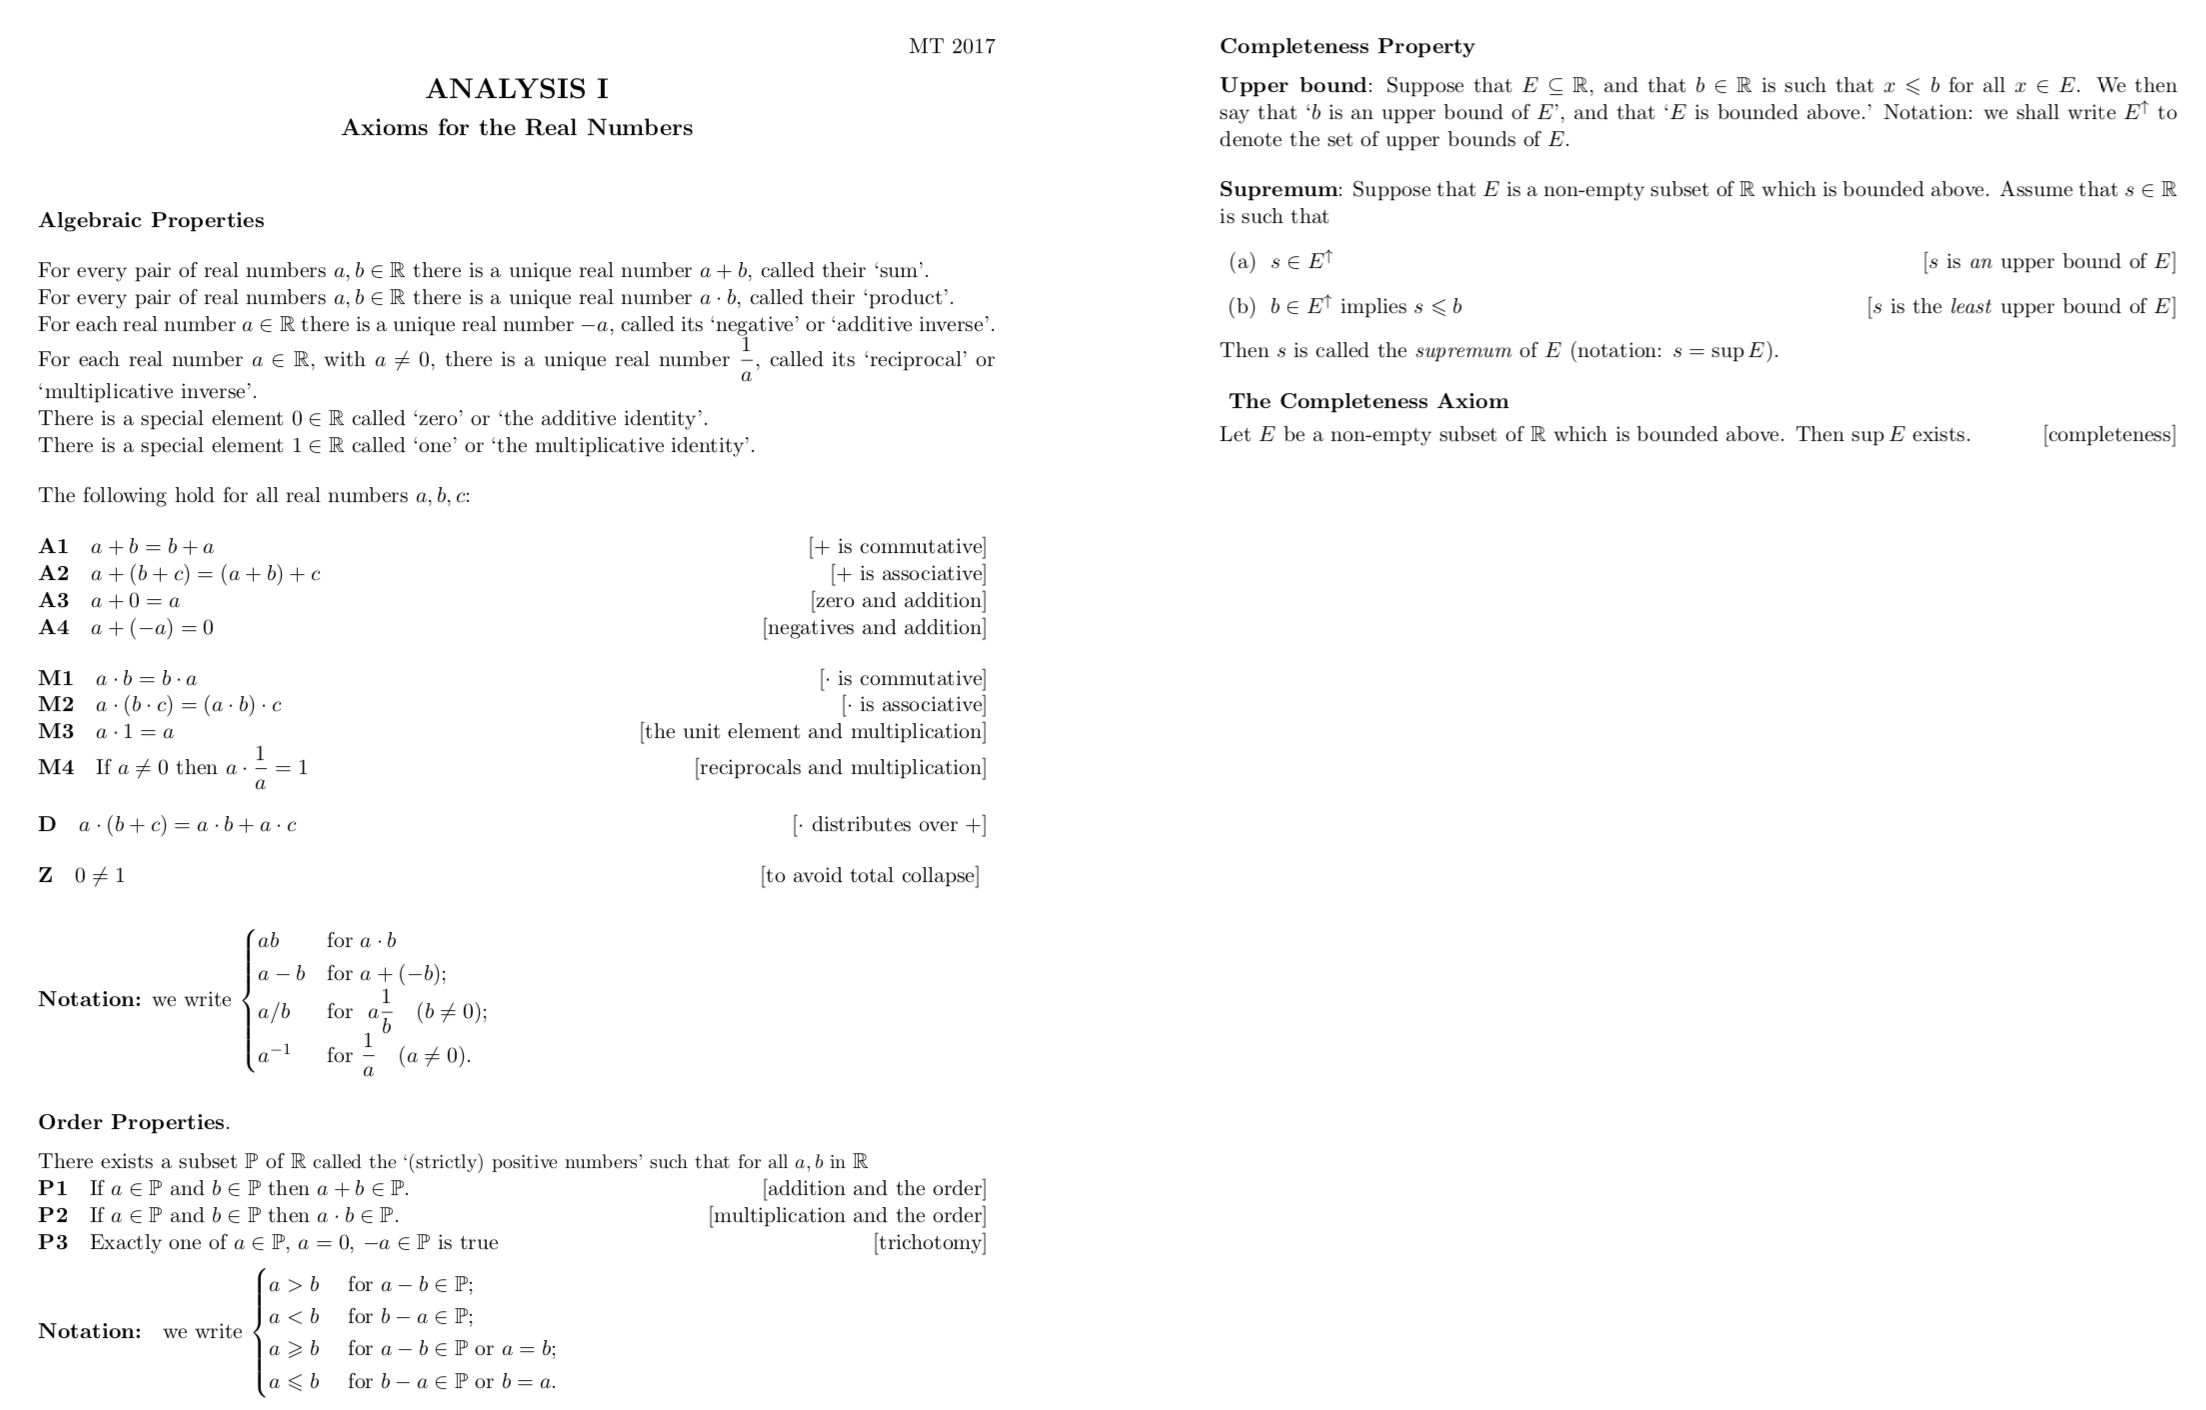
\includegraphics[width=400pt]{img/oxford-prelims-M2-analysis-I-axioms-for-real-numbers.png}
\end{mdframed}

\subsection{Approximation property of supremum}
\begin{theorem*}
  Let $S \subset \R$ be non-empty and bounded above (so $\sup S$ exists). For all $\delta > 0$,
  there exists $s_\delta \in S$ such that
  \begin{align*}
    \sup S - \delta < s_\delta \leq \sup S.
  \end{align*}
  \begin{intuition*}
    The supremum is either a member of $S$ or it is ``touching'' $S$ so that there is no gap.
  \end{intuition*}
  \begin{proof}
    If $\sup S \in S$ then we can take $s_\delta = \sup S$ for all $\delta$ and we are done.

    So assume $\sup S \not\in S$. For a contradiction, suppose the negation of the claim, i.e. that
    there exists $\delta > 0$ such that for all $s \in S$ either $s \leq \sup S - \delta$ or
    $s > \sup S$. Since $s > \sup S$ is impossible by definition of $\sup$, we have that
    $s \leq \sup S - \delta$ for all $s \in S$. But then $\sup S - \delta$ is an upper bound for
    $S$ and $\sup S - \delta < \sup S$, a contradiction.
  \end{proof}
\end{theorem*}

\subsection{Well-ordered property of $\N$}
\begin{theorem*}\hspace{0pt}
  Every nonempty subset of $\N$ has a minimum.
\end{theorem*}

\begin{remark*}
  Similarly:
  \begin{enumerate}
    \item Every nonsubset of $\Z$ that is bounded below has a minimum.
    \item Every nonsubset of $\Z$ that is bounded above has a maximum.
  \end{enumerate}
\end{remark*}

\begin{proof}
  This can be proved by considering $\N$ as a subset of $\R$, using completeness of $\R$ and
  applying the Approximation Property.
\end{proof}

\begin{intuition*}
  Because of the ``gappiness'' of $\N$ and $\Z$, bounded subsets must contain their suprema/infima.
\end{intuition*}

\subsection{Existence of $\sqrt 2$}
\begin{theorem*}
  There exists a unique $a \in \R$ such that $a^2 = 2$.
\end{theorem*}

\begin{remark*}
  The only thing that ties the proof to the reals is that it relies on completeness ($\sup$
  exists). We know that $\sqrt 2 \not\in \Q$, therefore $\Q$ is not complete.
\end{remark*}

\begin{proof}
  Let $S = \{s \in \R ~|~ s^2 < 2\}$. Since $S$ is bounded above, $a := \sup S$ exists. We show
  that $a^2 = 2$ by showing that $a^2 < 2$ and $a^2 > 2$ lead to contradictions.

  Note that $1 \in S$, therefore $a \geq 1$.

  \begin{enumerate}
  \item {\bf Suppose $a^2 < 2$}. We seek an $h > 0$ such that $(a + h)^2 < 2$ since this would
    contradict the definition $a := \sup S$. Note that
    \begin{align*}
      (a + h)^2 - 2 &= a^2 + 2ah + h^2 - 2\\
                    &< a^2 - 2 + 3ah ~~~~~~~\text{if $h < a$}\\
                    &< 0             ~~~~~~~~~~~~~~~~~~~~~~\text{if $h < (2 - a^2)/3a$}.
    \end{align*}
    Therefore if we take $h < \min\(a, \frac{2 - a^2}{3a}\)$ then $a + h \in S$ which contradicts
    the definition $a := \sup S$.
  \item {\bf Suppose $a^2 > 2$}. By the Approximation Property for all $0 < h < 1$ we can find
    $s \in S$ such that $a - h < s$.  Therefore $(a - h)^2 < s^2 < 2$. We seek a value of $h$ such
    that $(a - h)^2 \geq 2$, which would be a contradiction. Note that $a^2 - 2ah < (a - h)^2$. If
    we take $h = (a^2 - 2)/2a$ then we have $a^2 - 2ah = 2 < (a - h)^2 < 2$, the desired
    contradiction.
  \end{enumerate}

  Finally to show that $a$ is unique, suppose that there exists $b \in \R$ with $b^2 = 2$. Then
  $0 = a^2 - b^2 = (a + b)(a - b)$ therefore $a = b$.
\end{proof}

\subsection{Connection between sequences and functions}
\begin{theorem*}
  The following two statements are equivalent:
  \begin{enumerate}
  \item $f(x) \to L$ as $x \to a$.
  \item For every sequence $(x_n)$ such that $x_n \neq a$
    \begin{align*}
      \(\LimEq{x_n}{a}{n}{\infty}\) \implies \(\LimEq{f(x_n)}{f(a)}{n}{\infty}\)
    \end{align*}
  \end{enumerate}
\end{theorem*}

\subsection{Limit of product is product of limits}
\begin{theorem*}\label{limit-of-product}~\\
  Let $\limxa f(x) = L_f$ and $\limxa g(x) = L_g$. Then
  $\limxa f(x)g(x) = L_fL_g$.
\end{theorem*}

\begin{proof}
  Note that
  \begin{align*}
    \limxa f(x)g(x) &= \limxa \Big((f(x) - L_f)(g(x) - L_g) + L_fg(x) + L_gf(x) - L_fL_g\Big)\\
                    &= L_fL_g + \limxa (f(x) - L_f)(g(x) - L_g),
  \end{align*}
  so we need to show that $\limxa (f(x) - L_f)(g(x) - L_g) = 0$. Fix $\epsilon > 0$. Since
  $\limxa (f(x) - L_f) = \limxa (g(x) - L_g) = 0$, there exists $\delta$ such that whenever
  $|x - a| < \delta$
  \begin{align*}
    |(f(x) - L_f)| < \sqrt \epsilon ~~~\text{and}~~~|(g(x) - L_g)| < \sqrt \epsilon,
  \end{align*}
  therefore $|(f(x) - L_f)(g(x) - L_g) - 0| < \epsilon$ as required.
\end{proof}

\subsection{Limit of quotient is quotient of limits}
\begin{theorem*}~\\
  Let $\limxa f(x) = L_f$ and $\limxa g(x) = L_g \neq 0$. Then
  \begin{align*}
    \limxa \frac{f(x)}{g(x)} = \frac{L_f}{L_g}.
  \end{align*}
\end{theorem*}

\begin{proof}
  \red{TODO}
  \begin{align*}
    \limxa \frac{f(x)}{g(x)} - \frac{L}{M}
    = \limxa \frac{f(x)}{g(x)} - \frac{1}{g(x)} + \frac{1}{g(x)} - \frac{L}{M}
  \end{align*}

  Let $L_f = \limxa f(x)$ and $L_g = \limxa g(x) \neq 0$.

  Fix $\epsilon > 0$ and let $\delta_f$ and $\delta_g$ be such that
  \begin{align*}
    |x - a| < \delta_f \implies |f(x) - L_f| < \epsilon\\
    |x - a| < \delta_g \implies |g(x) - L_g| < \epsilon.
  \end{align*}
  Let $\delta = \min(\delta_f, \delta_g)$. Then
  \begin{align*}
    \frac{|f(x) - L_f|}{|g(x) - L_f|}
  \end{align*}
\end{proof}



\section{Exercises}

\subsection{Sheet 1}

\begin{enumerate}

\item
  \begin{enumerate}[label=(\alph*)]
  \item \begin{theorem*} $a(bc) = c(ba)$\end{theorem*}
    \begin{proof}
      \begin{align*}
        a(bc) &= a(cb)  ~~~~~~~ \text{(M1 commutativity of multiplication)}\\
              &= (ac)b  ~~~~~~~ \text{(M2 associativity of multiplication)}\\
              &= (ca)b  ~~~~~~~ \text{(M1 commutativity of multiplication)}\\
              &= c(ab)  ~~~~~~~ \text{(M2 associativity of multiplication)}\\
              &= c(ba)  ~~~~~~~ \text{(M1 commutativity of multiplication)}
      \end{align*}
    \end{proof}
  \item
    \begin{theorem*}
      $-(a + b) = (-a) + (-b)$
    \end{theorem*}
    \begin{proof}
      \begin{align*}
        (a + b) + (-(a + b))                   &= 0           ~~~~~~~ \text{definition of negative}\\
        \Big((-a) + (-b)\Big) + \Big((a + b) + (-(a + b))\Big) &= (-a) + (-b) ~~~~~~~ \text{add to both sides what axiom is this?}\\
        \Big((-b) + (-a)\Big) + \Big((a + b) + (-(a + b))\Big)   &= (-a) + (-b) ~~~~~~~ \text{S1 commutativity of sum}\\
        \Big(((-b) + (-a)) + (a + b)\Big) + (-(a + b))   &= (-a) + (-b) ~~~~~~~ \text{S2 associativity of sum}\\
        \Big((-b) + ((-a) + a) + b)\Big) + (-(a + b))    &= (-a) + (-b) ~~~~~~~ \text{S2 associativity of sum}\\
        \Big((-b) + (0 + b)\Big) + (-(a + b))            &= (-a) + (-b) ~~~~~~~ \text{definition of negative}\\
        \Big((-b) + b\Big) + (-(a + b))                &= (-a) + (-b) ~~~~~~~ \text{definition of 0}\\
        0 + (-(a + b))                         &= (-a) + (-b) ~~~~~~~ \text{definition of negative}\\
        -(a + b)                               &= (-a) + (-b) ~~~~~~~ \text{definition of 0}\\
      \end{align*}
    \end{proof}
  \end{enumerate}

\item
  \begin{enumerate}[label=(\alph*)]
  \item
    \newpage
    \begin{theorem*}
      If $a < b$ then $ac > bc$ iff $c < 0$.
    \end{theorem*}
    \begin{intuition*}
      Multiplication by a scalar flips orientation iff the scalar is negative.
    \end{intuition*}
    \begin{proof}~\\
      \red{TODO} Prove carefully being explicit about which axioms are used.\\
      Let $\P$ be the strictly positive reals. We have $a < b$, i.e. $b - a \in \P$.\\
      $\implies$:\\
      We have $ac > bc$ i.e. $ac - bc \in \P$.

      Therefore
      \begin{align*}
        (a - b)c &\in \P\\
        (b - a)(-c) &\in \P\\
        \frac{1}{b-a}(b - a)(-c) &\in \P\\
        (-c) &\in \P
      \end{align*}

      $\impliedby$:\\
      We have $c < 0$, i.e. $-c \in \P$. Therefore $(-c)(b - a) \in \P$ (by {\bf P2}). Therefore
      $ac - bc \in \P$, i.e. $ac > bc$.
    \end{proof}
  \end{enumerate}~\\
\item

  \begin{mdframed}
    \includegraphics[width=400pt]{img/oxford-prelims-M2-analysis-I-sheet-1-5.png}
  \end{mdframed}
\end{enumerate}

\newpage
\subsection{Sheet 2}

\begin{enumerate}
\item~\\
  \begin{mdframed}
    \includegraphics[width=400pt]{img/oxford-prelims-M2-analysis-I-sheet-2-1.png}
  \end{mdframed}
\item~\\
  \begin{mdframed}
    \includegraphics[width=400pt]{img/oxford-prelims-M2-analysis-I-sheet-2.png}
  \end{mdframed}
\item~\\
  \begin{mdframed}
    \includegraphics[width=400pt]{img/oxford-prelims-M2-analysis-I-sheet-2-3.png}
  \end{mdframed}

  \begin{intuition*}
    If there were an upper bound there would be a supremum. But if there were a supremum it would
    have to either be in the set or ``adjacent'' to the max value in the set.
  \end{intuition*}

  \begin{intuition*}[Incomplete proof]
    Let $S = \{2^n ~|~ n \in \N\}$ and suppose an upper bound for $S$ exists.

    Then $\sup S$ exists by completeness of the reals.

    Suppose $\sup S \in S$. Therefore $\sup S = 2^k$ for some $k$. But then $2^{k+1} \in S$ and
    $2^{k+1} > \sup S$, a contradiction.

    Alternatively, suppose $\sup S \not\in S$. [Informally, what we want to do now is show that
    this implies that $S$ has some maximum value $\max(S) < \sup S$, and that that leads to a
    contradiction. But how do we know that $S$ has a maximum? The easiest way to arrive at the
    required contradiction is via the Approximation Property of the supremum, which basically says
    that the supremum must be ``adjacent'' to $S$, with no gap. This gives rise to the following
    valid proof.]
  \end{intuition*}

  \begin{proof}
    Let $S = \{2^n ~|~ n \in \N\}$ and suppose an upper bound for $S$ exists.

    Then $\sup S$ exists by completeness of the reals.

    By {\bf 4.9} (Approximation Property of the supremum) there exists $2^k \in S$ such that
    \begin{align*}
      \sup S - \frac{1}{2} < 2^k \leq \sup S.
    \end{align*}
    Note that $k+1 \in \N$ therefore $2^{k+1} = 2^k + 2^k \in S$. Therefore
    \begin{align*}
      \sup S - \frac{1}{2} + 2^k &< 2^{k+1} \leq \sup S\\
      \sup S &\leq \sup S + \frac{1}{2} - 2^k < \sup S,
    \end{align*}
    a contradiction. Therefore no upper bound for $S$ exists.
  \end{proof}

\item~\\
  \begin{mdframed}
    \includegraphics[width=400pt]{img/oxford-prelims-M2-analysis-I-sheet-4.png}
  \end{mdframed}
  \begin{enumerate}
  \item $S = \Q \cap [0, \sqrt 2]$
    \begin{align*}
      \sup S &= \sqrt 2\\
      \max S &= \sqrt 2\\
      \min S &= 0\\
      \inf S &= 0
    \end{align*}
  \item $S = \{(-1)^n + 1/n ~|~ n=1,2,\ldots\}$
    \begin{align*}
      \sup S &= 3/2\\
      \max S &= 3/2\\
      \min S ~&\text{does not exist since $\inf S \not\in S$}\\
      \inf S &= -1
    \end{align*}
  \item $\{3^n ~|~ n \in \Z\}$
    \begin{align*}
      \sup S ~&\text{does not exist, $S$ has no upper bound}\\
      \max S ~&\text{does not exist, $S$ has no upper bound}\\
      \min S ~&\text{does not exist, $S$ has no lower bound}\\
      \inf S &= 0
    \end{align*}
  \item $\cup_{n=1}^\infty [\frac{1}{2n}, \frac{1}{2n - 1}]$
    \begin{align*}
      \sup S ~&= 1\\
      \max S ~&= 1\\
      \min S ~&\text{does not exist, $S$ has no lower bound}\\
      \inf S ~&=0
    \end{align*}
  \end{enumerate}

\item~\\
  \begin{mdframed}
    \includegraphics[width=400pt]{img/oxford-prelims-M2-analysis-I-sheet-5-a.png}
  \end{mdframed}

  \begin{proof}
    Let $S, T \subset \R$ with $S, T \neq \emptyset$. Assume that $S$ and $T$ are bounded
    above. Then $\sup S$ and $\sup T$ exist. Let $b = \max(\sup S, \sup T)$.

    Then $b \geq s$ for all $s \in S$ and $b \geq t$ for all $t \in T$. Therefore $b$ is an upper
    bound for $S \cup T$.

    Suppose there exists $a < b$ such that $a$ is an upper bound of $S \cup T$. Then either
    $a < \sup S$ or $a < \sup T$. Without loss of generality, suppose $a < \sup S$. Then $a$ is not
    an upper bound of $S$. Therefore there exists $s \in S$ such that $s > a$. But
    $s \in S \cup T$, therefore $a$ is not an upper bound of $S \cup T$, a contradiction.
  \end{proof}

  \begin{mdframed}
    \includegraphics[width=400pt]{img/oxford-prelims-M2-analysis-I-sheet-5-b.png}
  \end{mdframed}

  \begin{proof}
    Let $S, T \subset \R$ with $S, T \neq \emptyset$. Assume that $S$ and $T$ are bounded
    below. Then $\inf S$ and $\inf T$ exist. Define
    \begin{align*}
      S + T := \{s + t ~|~ s \in S, t \in T\}.
    \end{align*}
    Let $a = \inf S + \inf T$.

    We claim that $a$ is a lower bound for $S + T$, i.e. $u \geq a$ for all $u \in S + T$.

    Let $u \in S + T$. Then $u = s + t$ for some $s \in S, t \in T$. Therefore
    $$u = (\inf S + v) + (\inf T + w) = a + (v + w) \geq a$$ for some $v, w \geq 0$. Therefore $a$ is
    a lower bound for $S + T$ as claimed.

    We further claim that $a = \inf S + T$.

    Suppose for a contradiction that there exists $b > a$ such that $b$ is a lower bound for
    $S + T$. Then $$b = a + v + w = (\inf S + v) + (\inf T + w)$$ for some $v, w > 0$. Fix
    $0 < \delta < \min(v, w)$. By {\bf 4.9} (Approximation Property of the supremum/infimum) there
    exist $s \in S$ and $t \in T$ such that $\inf S \leq s < \inf S + \delta$ and
    $\inf T \leq t < \inf T + \delta$. But then $s + t \in S + T$ and $s + t < b$, so $b$ is not a
    lower bound for $S + T$, a contradiction. Therefore $a = \inf S + T$ as claimed.
  \end{proof}

  \newpage
\item~\\
  \begin{mdframed}
    \includegraphics[width=400pt]{img/oxford-prelims-M2-analysis-I-sheet-6.png}
  \end{mdframed}

  \begin{proof}
    Let $S = \{x \in \R ~|~ x^3 < 2\}$. Since $S$ is bounded above, $\sup S$ exists. Let
    $a = \sup S$. By trichotomy it suffices to show that $a^3 < 2$ and $a^3 > 2$ lead to
    contradictions.

    First suppose $a^3 < 2$. We seek $h > 0$ such that $(a + h)^3 < 2$ since then $a + h \in S$,
    which would contradict the definition $a := \sup S$. Note that
    \begin{align*}
      (a + h)^3 &= a^3 + 3a^2h + 3ah^2 + h^3 - 2\\
                &< a^3 + 7a^2h - 2 ~~~~~~~~~~~~~~~~~~~~~~~~\text{if $h < a$}\\
                &< 0              ~~~~~~~~~~~~~~~~~~~~~~~~~~~~~~~~~~~~~~~~~\text{if $h < \frac{2 - a^3}{7a^2}$},
    \end{align*}
    therefore if we take $h < \min\(a, \frac{2 - a^3}{7a^2}\)$ then we have the desired
    contradiction.

    Alternatively suppose that $a^3 > 2$. By the Approximation Property for all $0 < h < a$ we can
    find $s \in S$ such that $a - h < s$, therefore $(a - h)^3 < s^3$. We seek an $h$ for which
    $(a - h)^3 > 2$ since then we would have $s^3 > 2$ which would contradict the definition of
    $S$. Note that
    \begin{align*}
      (a - h)^3 - 2 &= a^3 - 3a^2h + 3ah^2 - h^3 - 2\\
                    &> 0 ~~~~~~~~~~~~~~~~~~~~~~~~~~~~~~~~~~~~~~~~~\text{if $3ah^2 > 3a^2h + h^3$}.
    \end{align*}
    So we require $3ah > 3a^2 + h^2 \iff 3a^2 - 3ah + h^2 < 0$.

    \red{incomplete}
  \end{proof}

  \newpage
\item~\\
  \begin{mdframed}
    \includegraphics[width=400pt]{img/oxford-prelims-M2-analysis-I-sheet-7-a.png}
  \end{mdframed}
  \begin{proof}
    $\R$ is uncountable. Since $\Q$ is countable, the irrationals $\R \setminus \Q$ must be
    uncountable.
  \end{proof}
  \begin{mdframed}
    \includegraphics[width=400pt]{img/oxford-prelims-M2-analysis-I-sheet-7-b.png}
  \end{mdframed}
  \begin{mdframed}
    \includegraphics[width=400pt]{img/oxford-prelims-M2-analysis-I-sheet-7-c.png}
  \end{mdframed}

\end{enumerate}


\newpage

\section{Continuity and Differentiability}
Note from Oxford - M2 - Continuity and Differentiability.

\subsection{Limit point}
\begin{definition*}
Let $E \subset \R$. A point $p \in \R$ is a limit point of $E$ iff for all $\delta > 0$ there
exists $x \in E$ such that $0 < |x - p| < \delta$.
\end{definition*}
\begin{intuition*}
  A deleted ball, of arbitrarily small radius, placed over $p$, will capture at least one point of
  $E$.
\end{intuition*}

\subsection{Limit, Convergence}

\begin{definition*}[Limit of a sequence $(x_n)$]~\\
$\LimEq{x_n}{L}{n}{\infty}$ iff for all $\epsilon > 0$ there exists an $m \in \N$ such that
$n > m \implies |x_n - L| < \epsilon$. The sequence is then said to \textit{converge} to $L$.
\end{definition*}

\begin{definition*}[Limit of a function $f:\R\to\R$]~\\
$\LimEq{f(x)}{L}{x}{a}$ means: for all $\epsilon > 0$ there exists $\delta > 0$ such that
$0 < |x - a| < \delta \implies |f(x) - L| < \epsilon$.
\end{definition*}

Equivalent notation: $f(x) \to L$ as $x \to a$

\begin{remark*}\hspace{0pt}
  \begin{enumerate}
  \item The value of $f$ at $a$ is irrelevant ($f$ need not be defined at $a$).
  \item $f$ must tend to $L$ from both sides.
  \end{enumerate}
\end{remark*}

\subsection{Continuity of a function $f$}

\begin{definition*}
$f$ is continuous at $a$ if $\LimEq{f(x)}{f(a)}{x}{a}$.
\end{definition*}

Therefore, using the definition of limit, $f$ is continuous at $a$ iff for all $\epsilon > 0$
there exists $\delta > 0$ such that $|x - a| < \delta \implies |f(x) - f(a)| < \epsilon$.

\subsection{Uniform convergence and uniform continuity}

\begin{definition*}[Uniform convergence]
A sequence of functions $\{f_n\}_{n\geq 0}$ has a limit $f$ iff for every point
$x$ in the input set the sequence $\{f_n(x)\}_{n\geq 0}$ has limit $f(x)$.

They \textit{converge uniformly} to $f$ iff the same $m$ works for all input
values.
\end{definition*}

\begin{definition*}[Uniform continuity]
A function $f$ is uniformly continuous iff the same $\delta$ works for all $x_0$.

A function $f$ is uniformly continuous iff for all $\epsilon$, no matter how
small, a $\delta$ exists such that for all $x_0 \in U$, if $x$ is within
$\delta$ of $x_0$ then $f(x)$ is within $\epsilon$ of $f(x_0)$.
\end{definition*}

\subsection{Intermediate value theorem}
\begin{theorem*}
  Let $a, b \in \R$ with $b > a$, and $f:[a,b] \to \R$ be continuous. Let $u$ lie strictly between
  $f(a)$ and $f(b)$. Then there exists $c \in (a, b)$ such that $f(c) = u$.
\end{theorem*}

\begin{proof}
  Define $S := \{x \in [a, b] ~|~ f(x) < u\}$. Since $a \in S$, $S$ is non-empty. By completeness
  of reals $c := \sup S$ exists. The theorem now follows from continuity of $f$ at $c$. (Fix
  $\epsilon > 0$ and consider points $a^* \in (c - \delta, c)$ and $a^{**} \in (c, c + \delta)$,
  noting whether they are in $S$ and the $\epsilon-\delta$ continuity criterion.)
\end{proof}


\subsection{Mean-value theorem}
\begin{theorem*}
  Let $a, b \in \R$ with $b > a$, and $f:[a,b] \to \R$ be continuous on $[a, b]$ and differentiable
  on $(a, b)$. Then there exists $x \in (a, b)$ such that $f'(x) = \frac{f(b) - f(a)}{(b - a)}$.
\end{theorem*}


\subsection{Differentiability implies continuity}
\begin{theorem*}
  Let $f:\R\to\R$ be differentiable. Then $f$ is continuous.
\end{theorem*}

\begin{proof}~\\
  Let $a \in \R$. The claim is that $\limxa f(x) - f(a) = 0$. Since $f$ is differentiable,
  \begin{align*}
    f'(a) &= \lim_{x \to a} \frac{f(x) - f(a)}{x - a}
  \end{align*}
  exists. Therefore by \eqref{limit-of-product}
  \begin{align*}
    \lim_{x \to a} f(x) - f(a) = \lim_{x \to a} (x - a)\frac{f(x) - f(a)}{x - a} = 0\cdot f'(a) = 0.
  \end{align*}
\end{proof}

\begin{remark*}
  Intuitively it seems that differentiability implies continuity because, for the derivative to
  exist, the numerator $f(x) - f(a)$ must get small as $x\to a$, as the denominator $x - a$ does.
\end{remark*}


\newpage
\section{Exercises}

\subsection{Limits of functions - Examples}

\begin{example}
  Let $E = \R\setminus \{0\}$ and define $f:E \to \R$ by $f(x) = L$. Then 0 is a limit point of
  $E$ and $f(x) \to L$ as $x \to 0$.
\end{example}

\begin{proof}
  Fix $\delta > 0$. Then $\exists x ~ 0 < |x - 0| < \delta$ is true since we can choose
  $x = \frac{\delta}{2}$. Therefore 0 is a limit point of $E$.

  Fix $\epsilon > 0$. Let $\delta = 1$. Then
  $0 < |x - 0| < \delta \implies |f(x) - L| = 0 < \epsilon$.
\end{proof}

\newpage
\subsection{Sheet 2}

\begin{mdframed}
  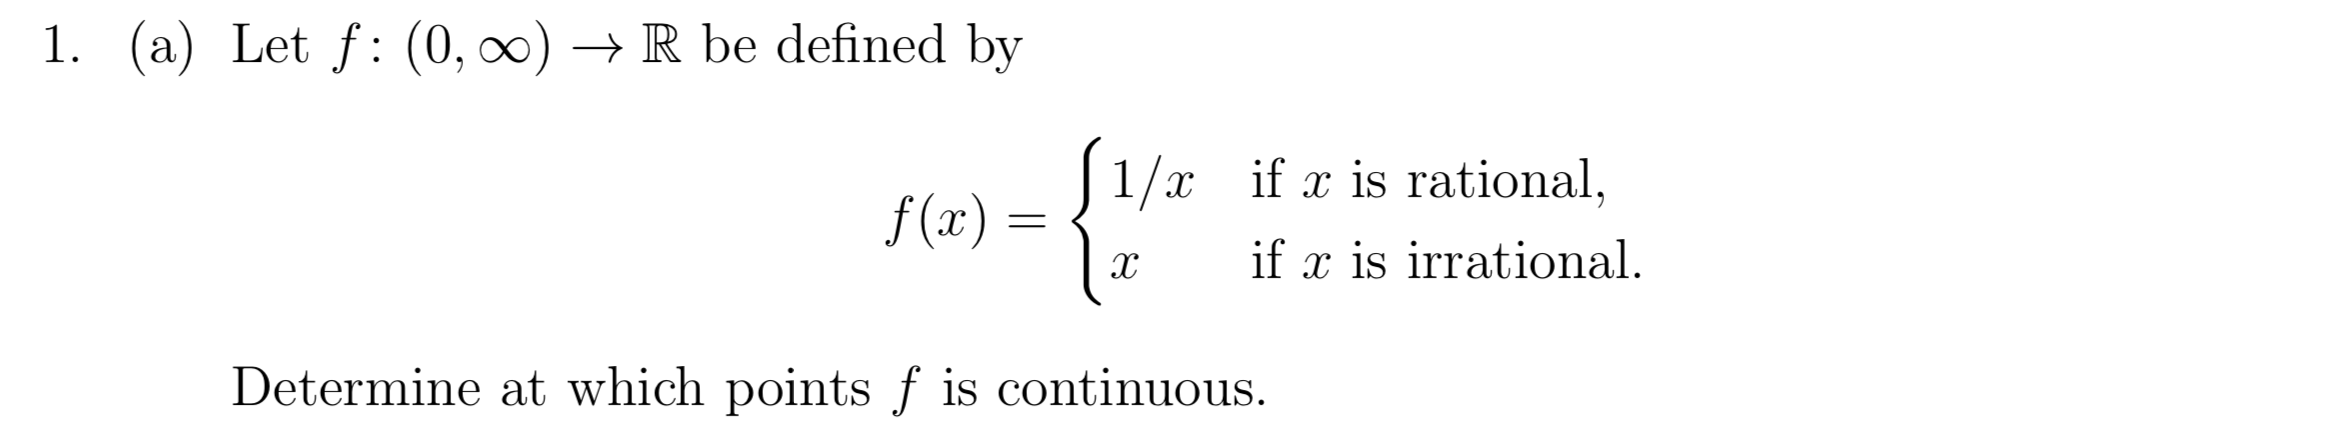
\includegraphics[width=400pt]{img/oxford-prelims-M2-analysis-II-sheet-2-1a.png}
\end{mdframed}

\begin{theorem*}
  $f$ is continuous at 1 and -1 only.
\end{theorem*}

\begin{proof} Let $q \in \Q \cap (0, \infty)$.

  Note that there exists a sequence $(q_n)$ such that $q_n \in \Q$, $q_n \neq q$ and
  $\LimEq{q_n}{q}{n}{\infty}$.

  From Theorem 1.13 (Algebra of Limits) we have $\Lim{x^\1}{x}{q} = q^\1$.

  Therefore from Theorem 1.10 we have

  % Therefore $\LimEq{f(q_n)}{1/q}{n}{\infty}$.

  Also, there exists a sequence $(p_n)$ such that $p_n \in \R\setminus\Q$, and
  $\LimEq{p_n}{q}{n}{\infty}$.


\end{proof}

\begin{definition*}[continuity]
  $f$ is continuous at $a$ if $\LimEq{f(x)}{f(a)}{x}{a}$.
\end{definition*}

\begin{definition*}[limit]
  $\LimEq{f(x)}{f(a)}{x}{a}$ if for all $\epsilon > 0$ there exists $\delta > 0$ such that
  $0 < |x - a| < \delta \implies |f(x) - f(a)| < \epsilon$.
\end{definition*}

\begin{theorem*}
  $f$ is continuous nowhere. I.e. for all $a \in (0, \infty)$ there exists $\epsilon > 0$ such that
  for all $\delta > 0$ there exists $x \in (0, \infty)$ such that $|x - a| < \delta$ and yet
  $|f(x) - f(a)| \geq \epsilon$.
\end{theorem*}

\begin{intuition*}
  However small we make $\delta$, an interval of radius $\delta$ centered at a rational point will
  contain irrational points, and vice versa.
\end{intuition*}

\begin{proof}~\\
  Let $x \in (0, \infty)$.

  Let $q \in \Q \cap (0, \infty)$. Then there exists a sequence:




  Fix $\delta > 0$. Note that there are both rational $x$ and
  irrational $x$ satisfying $0 < |x - q| < \delta$. Therefore the maximum value attained by
  $|f(x) - f(q)|$ is $||$
\end{proof}



Let $p \in (0, \infty) \setminus \Q$ be an

Let $p, q \in (0, \infty)$ with $p \notin \Q$ and $q \in \Q$.


\newpage
\section{Metric Spaces}

\subsection{Metric space}
\begin{definition}
  Let $X$ be a set. Suppose $d:X \times X \to \R$ satisfies positivity, symmetry and the triangle
  equality. Then $d$ is a metric and $(X, d)$ is a metric space.
\end{definition}

\subsection{Open ball}
\begin{definition}
  Let $(X, d)$ be a metric space, $x \in X$ and $\delta > 0$. Then
  $B(x, \delta) := \{x \in X ~|~ d(x, x) < \delta\}$ iss an open ball of radius $\delta$ centred at
  $x$.
\end{definition}

\begin{remark*}
  Also closed ball, $\leq$. E.g. singleton set.
\end{remark*}

\subsection{Ball-based continuity criterion}
\begin{lemma}
  $f$ is continuous at $x$ if for all $\epsilon > 0$ there exists $\delta > 0$ such that
  $f\(B(x, \delta)\) \subseteq B(f(x), \epsilon))$.

  Equivalently, $B(x, \delta) \subseteq f^\1\(B(f(x), \epsilon)\)$.
\end{lemma}

\subsection{Neighbourhood}
\begin{definition}
  Let $(X, d)$ be a metric space. $N \subseteq X$ is a neighbourhood of $x \in X$ iff there exists
  $\delta > 0$ such that $B(x, \delta) \subseteq N$.
\end{definition}

\begin{remark*}
  $N$ is a neighbourhood of $x$ if a ball can be placed at $x$ without poking outside $N$.
\end{remark*}

\subsection{Open and closed subsets of a metric space}
\begin{definition}
  Let $(X, d)$ be a metric space. Then $U \subseteq X$ is open iff it is a neighbourhood of all of
  its elements.

  $V \seq X$ is closed iff its complement in $X$ is open.
\end{definition}

\subsection{Topology on a metric space}
\begin{definition}
  Let $(X, d)$ be a metric space. The collection $\mc T$ of all open sets in the metric space is
  called the topology of $X$.
\end{definition}

\begin{remark*}
  Note that the definitions so far have the following dependency:

  (open set) $\larrow$ (neighbourhood) $\larrow$ (ball) $\larrow$ (metric),

  so they apply to metric spaces only.
\end{remark*}

\subsection{Open set-based continuity criterion}
\begin{theorem}
  Let $X$ and $Y$ be metric spaces and let $f:X \to Y$. Then

  $f$ is continuous at $x$ iff for every neighbourhood $N \subseteq Y$ of $f(x)$, the preimage
  $f^\1(N)$ is a neighbourhood of $x \in X$.

  $f$ is continuous iff for every open set $U$ of $Y$, $f^\1(U)$ is an open set of $X$.
\end{theorem}

\begin{remark*}
  So we have defined continuity in terms of open sets (the topology). This means that the metric is
  only relevant insofar as it induces the topology; two metric spaces with the same topology have
  the same notion of continuity.
\end{remark*}

\begin{proof}~\\
  Let $f$ be continuous at $x \in X$, and let $N \seq Y$ be a neighbourhood of $f(x)$.

  Then by definition of neighbourhood there exists a ball at $f(x)$ that stays within $N$.

  By continuity of $f$ the preimage of that ball is a superset of a ball at $x$.

  So the preimage of the ball is a neighbourhood of $x$. Therefore the preimage of $N$ is also.

  Conversely, ... similar.

  Let $f$ be continuous on $X$. Now every open set $U$ of $Y$ contains a ball around some point $y$...
\end{proof}

\subsection{Topology on a set, topological space}
\begin{definition}
  A topology on a set $X$ is a collection $\mc T$ of subsets of $X$, which are called the open
  sets. They must satisfy
  \begin{enumerate}
  \item closed under arbitrary unions. In particular, $\emptyset$ is an open set of $X$.
  \item closed under finite intersections. In particular, $X$ is an open set of $X$.
  \end{enumerate}
  A topological space is a pair $(X, \mc T)$.
\end{definition}

\begin{remark*}
  Criteria for closed sets follow by applying de Morgan's laws (closure under finite unions and
  arbitrary intersections).

  $f:X\to Y$ closed iff $f^\1(V)$ is closed for all closed sets $V \seq Y$.
\end{remark*}

\subsection{Limit point}
\begin{definition}
  Let $(X, d)$ be a metric space and $Z \seq X$ be any subset.

  $x \in X$ is a limit point of $Z$ if for all $\delta > 0$ the deleted open ball
  $B(x, \delta)\setminus\{x\}$ has non-empty intersection with $Z$.

  If $z$ is not a limit point of $Z$, then it is an isolated point.

  The set of limit points of $Z$ is denoted $Z'$, and it is clear that
  $Z_1 \seq Z_2 \implies Z_1' \seq Z_2'$.
\end{definition}

\begin{intuition*}
  $x \notin Z$ is a limit point of $Z$ iff it ``touches'' $Z$.

  $z \in Z$ is a limit point of $Z$ if it ``lies in a contiguous region of $Z$''

  An isolated point of $Z$ is what it sounds like.
\end{intuition*}

\begin{example*}~\\
  Let $Z = (0, 1] \cup \{2\}$.

  Intuitively, 0 is a limit point of $Z$ because it ``touches'' $Z$.

  Formally, 0 is a limit point of $Z$ because for all $\delta > 0$ the deleted open ball
  $B(0, \delta)$ contains a point $z > 0 \in Z$.

  Intuitively, 2 is an isolated point.

  Formally, 2 is not a limit point because $\(B(2, 0.5)\setminus\{2\}\) \cap Z = \emptyset$. And
  yet $2 \in Z$, therefore 2 is an isolated point.
\end{example*}

\subsection{Open sets theorems}
\begin{enumerate}
\item An open ball is open
\end{enumerate}

\subsection{Closed sets theorems}
\begin{enumerate}
\item A closed ball is closed
\end{enumerate}


\subsection{Continuity theorems}
\begin{enumerate}
\item $f:X \to Y$ is continuous if for every open ball in $Y$ there is an open ball in $X$ that
  maps inside it.
\item $f:X \to Y$ is continuous if the preimage of $B(f(x), \epsilon)$ in $Y$ is a ball
  $B(x, \delta)$ in $X$.
\item $f:X \to Y$ is continuous if the preimage of the neighbourhood of $f(x)$ is a neighbourhood
  of $x$.
\item $f:X \to Y$ is continuous if the preimage of every open set in $Y$ is an open set in $X$.
\end{enumerate}


\subsection{Continuity of a linear map}
\begin{theorem}
  Let $f:V \to W$ be a linear map between normed vector spaces. Then $f$ is continuous if and only
  if $\{\norm{f(x)} : \norm{x} \leq 1\}$ is bounded.
\end{theorem}

\begin{proof}~\\
  Let $v \in V$.

  Note that $f(v) = f(v) - f(0)$ since $f$ is linear.

  Suppose $f$ is continuous. Then it is continuous at 0.

  Therefore for every $\epsilon > 0$ there exists $\delta > 0$ such that
  $\norm{v} < \delta \implies \norm{f(v)} < \epsilon.$

  $\vdots$

  For the converse, suppose that $\norm{v} \leq 1 \implies \norm{f(v)} < M$.

  Let $\epsilon > 0$ be given.

  Pick $\delta > 0$ such that $\delta M < \epsilon$.

  Now consider two points $u, v \in V$ where $\norm{u - v} < \delta$. We have
  \begin{align*}
    \norm{f(u) - f(v)} = \norm{f(u - v)} = \delta\norm{f\(\frac{u - v}{\delta}\)}.
  \end{align*}

  Note that $\norm{\frac{u - v}{\delta}} < 1$, therefore $\norm{f\(\frac{u - v}{\delta}\)} <
  M$. Therefore we have
  \begin{align*}
    \norm{f(u) - f(v)} < \delta M < \epsilon
  \end{align*}
  as required.
\end{proof}

\subsection{Norm of linear map is bounded}
\begin{theorem}
  $\{\norm{f(x)} : \norm{x} \leq 1\}$ is bounded for linear map $f$, under the Euclidean norm
  $\norm{}_2$.
\end{theorem}

\begin{proof}
  See Oxford A2 Sheet 1 exercises.
\end{proof}


\chapter{Measure Theory and Topology}
\section{Billingsley Section 1}
[Berkeley 202a]
[Billingsley - Probability \& Measure]

Why does he say ``closed under countable unions and intersections.​''?

  Billingsley p.19:
  \begin{quote}
    ...require a collection that contains the intervals and is closed under countable unions and intersections.
    Note that a singleton $\{x\}$ is a countable intersection of intervals:
    \begin{align*}
      \bigcap_{n=1}^\infty \Big(x -\frac{1}{n}, x\Big] = \{x\}.
    \end{align*}
  \end{quote}


\begin{itemize}
\item $\Omega = [0, 1]$
\item $\om \in \Omega$
\item $d_n(\om) \in \{0, 1\} = $ $n$-th digit in binary expansion of $\om$
\item Rademacher function $r_n(\om) = 2d_n(\om) - 1 \in \{-1, 1\}$
\end{itemize}

\subsection{Weak Law of Large Numbers}

Define the partial sum $s_n(\om) = \sum_{i=1}^n r_i(\om)$, i.e. the number of $1$s minus the number of $0$s in
the first $n$ digits of the binary expansion of $\om$. (The displacement of the random walk after $n$ steps.)

\begin{lemma}
  \begin{align*}
    \int_0^1 s_n(\om)^2 \d\om = n
  \end{align*}
\end{lemma}

I.e., viewed as a sequence of $n$ coin tosses yielding $-1$ or $+1$, the variance (expected squared distance
from mean) of their sum is $n$.

\begin{proof}
  Note that $s_n(\om)^2 = \sum_{i=1}^n r_i(\om)^2 - 2\sum_{i<j}r_i(\om)r_j(\om)$. Integrating over $[0, 1]$ we have
  \begin{align*}
    \int_0^1 s_n(\om)^2 \d\om
    &= \sum_{i=1}^n \int_0^1 r_i(\om)^2 \d\om - 2\sum_{i<j}\int_0^1r_i(\om)r_j(\om) \d\om \\
    &= \sum_{i=1}^n \int_0^1 1 \d\om - 0 \\
    &= n.
  \end{align*}
  We used there the fact that $\int_0^1r_i(\om)r_j(\om) \d\om = 0$ for $i < j$, i.e that the Rademacher
  functions are orthogonal. An argument for this is that as we move through a rank $i$ dyadic
  interval, $r_i(\omega)$ is constant (either $-1$ or $+1$) while at rank $j$ below, $r_j(\omega)$ flickers
  between $-1$ and $+1$, spending an equal amount of time in each.
\end{proof}


\begin{lemma}[Markov's Inequality]
  Let $f: [0, 1] \to \R^+$ be a step function. Then
  \begin{align*}
    P\Big(\Big\{x: f(x) \geq \alpha\Big\}\Big) \leq \frac{1}{\alpha}\int_0^1 f(x) \dx.
  \end{align*}
\end{lemma}




\begin{intuition}
  Think of the statement in rearranged form:
  \begin{align*}
    \alpha P\Big(\Big\{x: f(x) \geq \alpha\Big\}\Big) \leq \int_0^1 f(x) \dx.
  \end{align*}



  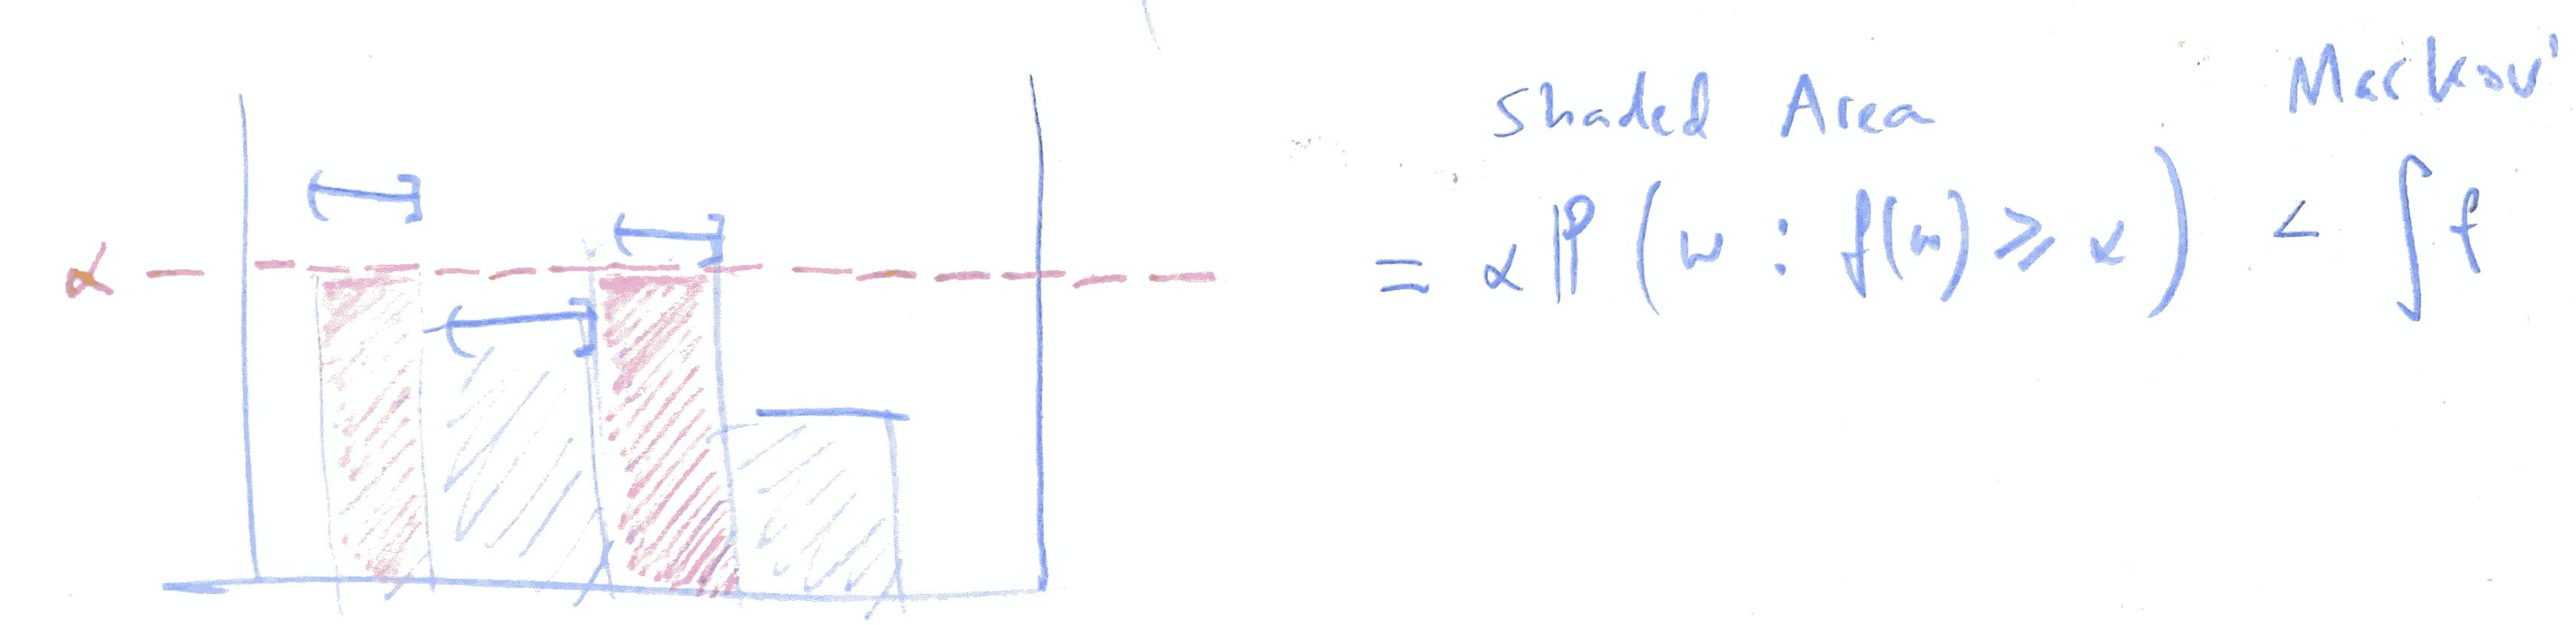
\includegraphics[width=400pt]{img/analysis--real-analysis--measure-theory--weak-law-of-large-numbers-c9c2.png}

  If $X \sim \Unif(0, 1)$ then the RHS is $\E[X]$.

\end{intuition}


\begin{proof}
  [me]

  Clearly
  \begin{align*}
    \int_{f(x) \geq \alpha} f \leq \int_{[0, 1]} f.
  \end{align*}
  Therefore
  \begin{align*}
    \int_{f(x) \geq \alpha} \alpha \leq \int_{[0, 1]} f
  \end{align*},
  or equivalently
\begin{align*}
  \alpha \int \textbf{1}_{f(x) \geq \alpha} \leq \int_{[0, 1]} f,
\end{align*}
which is the same thing as
  \begin{align*}
    \alpha P\Big(\Big\{x: f(x) \geq \alpha\Big\}\Big) < \int_0^1 f(x) \dx.
  \end{align*}
\end{proof}

\begin{theorem}[Weak Law of Large Numbers]
  Fix an $\epsilon > 0$. Then
  \begin{align*}
    \lim_{n \to \infty}P\Big(\Big\{\om: \frac{1}{n}\big|\sum_{i=1}^n r_i(\om)\big| \geq \epsilon\Big\}\Big) = 0.
  \end{align*}
\end{theorem}

In other words: we move through all the $\om \in [0, 1]$. For a given $\om \in [0, 1]$, compare the number
of $0$s and $1$s in the first $n$ digits of the binary expansion, and record the excess as a proportion of $n$;
this is $\frac{1}{n}|s_n(\om)|$. The theorem states that for all $\epsilon > 0$ the probability measure
associated with the set of $\om$s for which $\frac{1}{n}|s_n(\om)| > \epsilon$ goes to $0$ as $n \to \infty$.

\begin{proof}
  Fix an $\epsilon > 0$. We square both sides of the inequality, instead of working with the absolute value. So
  what we want to show is that $P\big(\big\{\om: s_n^2(\om) \geq n^2\epsilon^2\big\}\big) \to 0$
  as $n \to \infty$.

  It would be nice to find an expression for this probability measure as a function of $n$. However, what we'll
  do is find an upper bound: that will suffice also.

  Note that $s_n(\om)$ is a step function (and so $s_n^2(\om)$ is also):

\includegraphics[width=200pt]{img/analysis--real-analysis--measure-theory--weak-law-of-large-numbers-c049.png}


By Markov's inequality / ``Shaded Area lemma​'' we have
\begin{align*}
  n^2\epsilon^2P\Big(\Big\{\om: s_n^2(\om) \geq n^2\epsilon^2\Big\}\Big) \leq \int_0^1 s_n^2(\om) \d\om = n
\end{align*}
and therefore
\begin{align*}
  P\Big(\Big\{\om: s_n^2(\om) \geq n^2\epsilon^2\Big\}\Big) \leq  \frac{1}{n\epsilon^2},
\end{align*}
which proves the desired result since it shows that the probability measure is bounded above by a quantity that
goes to $0$ as $n \to \infty$.
\end{proof}

\subsection{Strong Law of Large Numbers}

\red{TODO} Relation of Borel's normal number theorem to SLNN.

\begin{definition}[negligible, null set]
  A set $A$ is \defn{negligible} if, for any $\epsilon > 0$, it can be covered by a finite or countable
  union $\bigcup_k I_k$ of intervals with $\sum_k |I_k| < \epsilon$.
\end{definition}

Recall the weak law of large numbers:
  \begin{align*}
    \lim_{n \to \infty}P\Big(\Big\{\om: \frac{1}{n}\big|s_n(\om)\big| \geq \epsilon\Big\}\Big) = 0.
  \end{align*}

\begin{definition}[Normal numbers]
  Define the set of \defn{normal numbers} to be
  \begin{align*}
    N = \Big\{\om ~:~ \lim_{n\to\infty} \frac{1}{n}s_n(\om) = 0 \Big\}.
  \end{align*}
\end{definition}

\begin{theorem*}[Borel's normal number theorem]
  $N^c = \R \setminus N$ is negligible.
\end{theorem*}

\begin{intuition}
  Note that the set of normal $\om$ can be written as the set of $\om$ that

  ``eventually stay within $1$​'' AND
  ``eventually stay within $1/2$'' AND
  ``eventually stay within $1/3$'' AND
  ``eventually stay within $1/4$'' ...
  \begin{align*}
    N = \bigcap_{k=1}^\infty \bigcup_{m=1}^\infty\bigcap_{n \geq m} \big\{ \om ~:~ \big|\frac{1}{n}S_n(\om)\big| < \frac{1}{k} \big\}.
  \end{align*}

  Visualize the $s_n$ sequence of a non-normal number $\om$, stretching off to infinity. However far we’ve
  gone, there will always be another point further along at which an excursion of the random walk sticks out
  further than $\eps$. But despite the fact that this must always happen, it’s less and less likely the further
  we go. The fact that it must always happen again corresponds to the fact that we can write the event as a
  countable union: (happened by this generation) union with (happened at the next generation), etc. But at the
  same time, since it’s getting harder and harder, for any given $\gamma >0$ we can find some generation $m$
  beyond which the union sums to less than $\gamma$. nevertheless , the event is equal to the union beyond that
  point, since the departures must always keep occurring (otherwise the number would be normal). So the union
  doesn’t have to include earlier generations.

  This is why the complement of the normal numbers is negligible. Perhaps it’s typical of negligible sets that
  they correspond to an event that must always occur one more time, and yet get ever less and less likely?
\end{intuition}

\begin{proof}
  Let $(\eps_n)$ be a sequence that converges to zero, and define a sequence of sets $(A_n)$, where
  \begin{align*}
    A_n = \Big\{\om : \Big|\frac{1}{n} s_n(\om)\Big| \geq \eps_n\Big\}.
  \end{align*}
  (We can think of $A_n$ as the set of $\om$ whose binary expansions are ``not normal so far​''.)

  Note that, for any given $m$, we have the following: a number that stays inside $\eps_n$ for ever is normal:
  \begin{align*}
    \Big(\bigcap_{n=m}^\infty A_n^c\Big) \subset N.
  \end{align*}
  Equivalently, a non-normal number must stray outside $\eps_n$ at some point:
  \begin{align*}
    N^c \subset \Big(\bigcup_{n=m}^\infty A_n\Big).
  \end{align*}
  Recall that our aim is to cover $N^c$ with a countable union of intervals, where the total length of the
  intervals is arbitrarily small (an ``efficent covering​​''). If we can show that the $A_n$ meet that
  description then we are done.

  Recall that $s_n$ is a step function such that, if $\om \in A_n$ then $\om' \in A_n$ for every $\om'$ in the
  same rank-$n$ dyadic interval as $\om$. Therefore each set $A_n$ is a finite disjoint
  union $\bigcup_{k}I_{nk}$ of intervals, and $P(A_n) = \sum_k |I_{nk}|$.

  So what we need to do is show that, for any given $\gamma > 0$, there exists a sequence $(\eps_n)$ converging
  to zero, and an $m$, such that $\sum_{n=m}^\infty P(A_n) < \gamma$.

  At this point, we need to find an expression for an upper bound on $P(A_n)$ in terms of $n$ and $\eps_n$.
  From the lemma, we have
  \begin{align*}
    P(A_n) \leq \frac{3}{n^2\eps_n^4},
  \end{align*}
  so we would like to find $(\eps_n)$ and $m$ such that
  \begin{align*}
    \sum_{n=m}^\infty \frac{3}{n^2\eps_n^4} < \gamma.
  \end{align*}
  To do so, we need only choose $(\eps_n)$ so that the series $\sum_nn^{-2}\eps_n^{-4}$
  converges: $\eps_n = n^{-1/8}$ will do. Then, since the series converges, there exists an $m$ such that the
  tail sums to less than $\gamma$, as required.
\end{proof}

\begin{lemma}
  Let $A_n = \Big\{\om : \Big|\frac{1}{n} s_n(\om)\Big| \geq \eps\Big\}$.

  For all $n \in \N$, we have (by taking the 4th power of both sides of the inequality and applying Markov's
  inequality)
  \begin{align*}
    P(A_n) \leq \frac{1}{n^4\eps^4} \int_0^1 s_n^4(\om) \d\om,
  \end{align*}
  and (by considering integrals of products of four Rademacher functions)
  \begin{align*}
    \int_0^1 s_n^4(\om) \d\om \leq 3n^2.
  \end{align*}
  Therefore
  \begin{align*}
    P(A_n) \leq \frac{3}{n^2\eps^4}.
  \end{align*}
\end{lemma}

\newpage
\subsection{An interval of  positive length is not negligible}

\begin{definition*}[length of an interval]
  The \defn{length} of $(a, b)$ is $|(a, b)| = b - a$.
\end{definition*}

\begin{theorem*}
  Let $I$ be an interval of positive length and let $I_1, I_2, \ldots$ be intervals.
  \begin{enumerate}
  \item If $\bigcup_k I_k \subseteq I$ (disjoint) then $\sum_k |I_k| \leq |I|$
  \item If $\bigcup_k I_k \supseteq I$ then $\sum_k |I_k| \geq |I|$. I.e. no cover of $I$ is negligible.
  \end{enumerate}
  A corollary is that if $\bigcup_k I_k = I$ then $\sum_k |I_k| = |I|$.
\end{theorem*}

\begin{proof}
  Let $I = (a, b)$ and let $I_k = (a_k, b_k)$ for all $k$.

  First, we show that if $\bigcup_k I_k \subseteq I$ (with the $I_k$ disjoint) then $\sum_k |I_k| \leq |I|$.

  There are two cases:
  \begin{enumerate}
  \item {\bf Finite cover}:

    The claim is that for any collection of $n$ disjoint intervals, if $\bigcup_{k=1}^n I_k \subseteq I$
    then $\sum_{k=1}^n |I_k| \leq |I|$.

    This is clearly true for a collection of intervals of size $n = 1$.

    Assume it's true for any collection of intervals of size $n-1$, and consider a collection of $n$ disjoint
    intervals with $\bigcup_{k=1}^n I_k \subseteq I$.

    Label the intervals $I_1, \ldots, I_n$, sorted by their left endpoint in ascending order. Note that the
    union of the first $n-1$ intervals is contained within $(a, a_n)$ and that the $n$-th interval has
    length $b_n - a_n \leq b - a_n$. Thus we have
    \begin{align*}
      \sum_{k=1}^n |I_k|
      &= \sum_{k=1}^{n-1}|I_k| + |I_n| \\
      &\leq (a_n - a) + (b - a_n) \\
      &= b - a.
    \end{align*}
    Therefore it is true for all $n$ by induction.

  \item {\bf Infinite cover}:

    The claim is that for any countably infinite collection of $n$ disjoint intervals,
    if $\bigcup_{k=1}^\infty I_k \subseteq I$ then $\sum_{k=1}^\infty |I_k| \leq |I|$.

    Consider an infinite collection of intervals satisfying $\bigcup_{k=1}^\infty I_k \subseteq I$.

    Note that for every finite subcollection of size $n$ we have $\sum_{k=1}^n |I_k| \leq |I|$ by the finite case.

    Therefore $\sum_{k=1}^\infty |I_k| = \sup \sum_{k=1}^n |I_k| \leq |I|$ where the supremum is over the set
    of all finite subcollections. Since this set is non-empty, the supremum is a finite positive number.
  \end{enumerate}
  ~\\~\\
  Finally, we show that if $\bigcup_k I_k \supseteq I$ then $\sum_k |I_k| \geq |I|$.
  Again, there are two cases:
  \begin{enumerate}
  \item {\bf Finite cover}:

    The claim is that for any collection of $n$ intervals, if $\bigcup_{k=1}^n I_k \supseteq I$
    then $\sum_{k=1}^n |I_k| \geq |I|$.

    In other words, that the total length of a finite cover of $I$ is bounded below by $|I| > 0$.

    Again, it's obvious for a cover comprising a single interval ($n=1$).

    Assume it's true for any cover comprising $n-1$ intervals, and consider a cover comprising $n$ intervals.

    Again, label the intervals $I_1, \ldots, I_n$, sorted by their left endpoint in ascending order.

    Note that the first $n-1$ intervals cover the interval $(a, b_{n-1})$ and that $|I_n| \geq b - b_{n-1}$.
    Thus we have
    \begin{align*}
      \sum_{k=1}^n |I_k|
      &= \sum_{k=1}^{n-1}|I_k| + |I_n| \\
      &\geq (b_{n-1} - a) + (b - b_{n-1}) \\
      &= b - a.
    \end{align*}

  \item {\bf Infinite cover}\\

    The claim is that for any infinite cover $\bigcup_{k=1}^\infty I_k \supseteq I$ we have $\sum_{k=1}^\infty |I_k| \geq |I|$.

    Consider a countably infinite cover of $I$.

    We might think that we could make an argument analogous to the one above:

    Note that for every finite subcover of size $n$ we have $\sum_{k=1}^n |I_k| \geq |I|$.

    Therefore $\sum_{k=1}^\infty |I_k| = \inf \sum_{k=1}^n |I_k|  \geq |I|$ where the infimum is over the set of all finite subcovers.

    However, we have to show that a finite subcover exists; otherwise the infimum would be $+\infty$.

    So what we do is construct a closed interval $[a + \eps, b]$ which is covered by a countably infinite open
    cover. Since that closed interval is compact from Heine-Borel, there exists a finite open subcover.

    \begin{quote}
      I think your second statement is true except for an infinite open cover of (a, b] which has finite total
      measure, but no finite subcovers. Such a cover does exist, and it’s the the object I was (clumsily)
      trying to refer to. So I think your second statement is false, but not nonsense, as it fails for the same
      reason that the second proof is more difficult.
    \end{quote}
  \end{enumerate}
\end{proof}


\begin{theorem}
  Every proper open subset of $\R$ is a countable union of disjoint open intervals and open rays.
\end{theorem}
\begin{proof}
  HW2 Q1 (uses an equivalence relation to partition the open set), Billingsley Example 2.6 (uses an
  uncountable union of intervals with rational endpoints which must contain duplicates).
\end{proof}


\begin{proof}
  Let $\ms A$ be a finite class of $n$ sets. Taking complements gives $2n$ sets.

  In the first iteration, each set can be involved in $2n$ unions and $2n$ intersections, for a total of $4n$
  new sets, which becomes $8n$ on taking complements.

  So after $k$ generations, we


\end{proof}
\subsection{sigma-algebras, Borel sets}

\url{https://en.wikipedia.org/wiki/Outcome_(probability)}


An \defn{outcome} is an atomic, lowest-level, result of an experiment/process. Outcomes are mutually exclusive.

An \defn{event} is a set of \defn{outcomes} that we assign probability to. It is a subset of $\Omega$. Events are not mutually
exclusive: ``greater than 0.5?​'' and ``greater than 0.6?​'' are both events and, for a given outcome, both events
may ``occur​''.

An \defn{algebra} is a collection of events. So an algebra contains all the things we might assign probability to.
Furthermore, an algebra must be closed under complementation, union and intersection ( ``not​'', ``or​'', and ``and​'').

A $\sigma$-\defn{algebra} is an algebra that is closed under countably infinite unions and intersections.

\begin{theorem}
  An open set is a {\it countable} union of disjoint intervals.
\end{theorem}

\begin{definition*}[$\sigma$-algebra]
  An \defn{algebra} in $\Omega$ is a collection of subsets of $\Omega$ that
  \begin{enumerate}
  \item contains $\emptyset$ and $\Omega$
  \item is closed under complements
  \item is closed under {\it finite} unions and intersections
  \end{enumerate}

  It is a $\sigma$-\defn{algebra} if it is additionally closed under {\it countable} unions and intersections.
\end{definition*}

\begin{definition}
  A ($\sigma$-) algebra \defn{generated} by a collection of subsets is the smallest ($\sigma$-) algebra of which that
  collection is a subset.
\end{definition}


\begin{quote}
  the intersection of all fields in $\Omega$ containing $\ms A$.
\end{quote}

Here, ``containing​'' means subset inclusion.

An in fact, ``in​'' here means neither set membership nor subset inclusion. It is used in a more technical sense
to refer to fields whose sets are subsets of $\Omega$ (i.e. fields that are elements of the powerset
of $\Omega$). Bass uses ``on​'' for this: ``a field on $\Omega$​''.

\begin{definition}[Borel $\sigma$-algebra, Borel set]
  A \defn{Borel} $\sigma$-\defn{algebra} is the $\sigma$-algebra generated by the open sets.

  A \defn{Borel set} is a subset of $\Omega$ that is an element of a Borel $\sigma$-algebra.
\end{definition}

A Borel $\sigma$-algebra contains is generated by open sets (and so equivalently by closed sets). But
the $\sigma$-algebra contains singletons, half-closed intervals, etc.

\begin{theorem}
  The Borel $\sigma$-algebra on $\R$ can be generated by the following sets
  \begin{enumerate}
  \item $\ms I_1 = \{(a, b) ~:~ a, b \in \R\}$
  \item $\ms I_2 = \{[a, b] ~:~ a, b \in \R\}$
  \item $\ms I_3 = \{(a, b] ~:~ a, b \in \R\}$
  \item $\ms I_4 = \{[a, \infty) ~:~ a \in \R\}$
  \item $\ms I_5 = \{(p, q) ~:~ p, q \in \Q\}$
  \end{enumerate}
\end{theorem}

\begin{proof}
  Let $\ms O$ be the collection of open subsets of $\R$, so that $\ms B = \sigma(\ms O)$.
  \begin{enumerate}
  \item The key here is that every open subset of $\R$ is a countable union of open intervals. So the collection of
    open sets is automatically in the $\sigma$-algebra generated by the open intervals, so you can't ``get
    anything new​'' from them.

    Let $\ms I_1 = \{(a, b) ~:~ a, b \in \R\}$. We want to show that $\sigma(\ms I_1) = \sigma(\ms O)$.

    In one direction, every element of $\ms I_1$ is open, so clearly $\sigma(\ms I_1) \subseteq \sigma(\ms O)$.

    For the other direction, let $X \in \ms O$ be an open subset of $\R$. Then $X$ is a countable union of open
    intervals (i.e. finite intervals and open rays). Every finite interval is in $\ms I_1$. But open ray are
    also countable unions of finite intervals: $(-\infty, a) = \bigcup_n^\infty (a-n, a)$
    and $(a, \infty) = \bigcup_n^\infty (a, a + n)$. Therefore $X \in \sigma(\ms I_1)$, i.e. every open set is
    in the $\sigma$-algebra generated by open intervals. This is equivalent to the
    statement $\ms O \subseteq \sigma(\ms I_1)$, i.e. the collection of all open sets is a subset of
    that $\sigma$-algebra. Therefore $\sigma(\ms O) \subseteq \sigma(\sigma(\ms I_1)) = \sigma(\ms I_1)$.

  \item We reduce this to (1) by showing that we can make $(a, b)$ from $[a, b]$.

    Let $\ms I_2 = \{[a, b] ~:~ a, b \in \R\}$. We want to show that $\sigma(\ms I_2) = \sigma(\ms O)$.

    To show $\sigma(\ms I_2) \subseteq \sigma(\ms O)$, note that for $a < b$
    \begin{align*}
      [a, b] &= \bigcap_{n=1}^\infty (a - n^{-1}, b + n^{-1}).
    \end{align*}
    Therefore $[a, b] \in \sigma(\ms I_1)$ for all $a, b \in \R$, hence $\sigma(\ms I_2) \subseteq \sigma(\ms I_1) = \sigma(\ms O)$.

    To show $\sigma(\ms O) \subseteq \sigma(\ms I_2)$, note that for $a < b$ and $n_0 \geq 2/(b - a)$
    \begin{align*}
      (a, b) &= \bigcup_{n=N_0}^\infty [a + n^{-1}, b - n^{-1}].
    \end{align*}
    Therefore $(a, b) \in \sigma(\ms I_2)$ for all $a, b \in \R$ hence $\ms I_1 \subseteq \sigma(\ms I_2)$,
    hence $\sigma(\ms I_1) = \sigma(\ms O) \subseteq \sigma(\ms I_2)$. But we have already shown
    that$\sigma(\ms I_1) = \sigma(\ms O)$, therefore $\sigma(\ms O) \subseteq \sigma(\ms I_2)$.
  \end{enumerate}
\end{proof}

\subsection{Bass 3. Measures}

Let $\Omega$ be a set and $\mc A$ a $\sigma$-algebra on $\Omega$.

A \defn{measure} is a function $\mu:\mc A \to [0, \infty]$ that is \defn{countably additive} (CA; measure of disjoint union equals sum of measures).

CA has various implications which make $\mu$ behave in unsurprising ways:
\begin{enumerate}
\item It's finitely and countably \defn{subadditive} (measure of union does not exceed sum of measures)
\item Measure of limiting sets equals limit of measures (e.g. if $A_i \uparrow A$ then $\mu(A) = \lim_n \mu(A_i)$)
\end{enumerate}

\begin{intuition*}
  The function $\mu$ is a map from sets to reals. So in principle it could assign whatever real values it wants
  to whatever sets. E.g. for disjoint $A, B$ it could assign a value to $\mu(A \cup B)$ that is completely
  different from $\mu(A) + \mu(B)$.

  In fact, however, measures treat sets as an aggregate of points. I think that everything is perfectly
  intuitive except that countably infinite unions might not work as expected.

  In other words, $\mu$ acts exactly as one would expect: as if it's applying a uniform layer of paint to each
  subset: the total amount of paint used to paint a union of disjoint sets is the sum of the paint applied to
  each set in the union.

  But CA means the additivity is retained even when there are infinitely many sets in the union. An example of CA
  failing to hold is densities of finite subsets of the natural numbers: the density of the singleton $\{1\}$ as
  a proportion of the natural numbers is naturally defined to be $0$ (the limit of the density in a finite sample
  as the sample size tends to infinity). But the density of the countable union of all singletons is $1$, which is
  not the sum of the densities.
\end{intuition*}

A measure is \defn{finite} if $\mu(\Omega) < \infty$, and $\sigma$\defn{-finite} if there exists a countable partition
of $\Omega$ with each subset in the partition having finite measure.

$(\Omega, \mc A, \mu)$ is a \defn{measure space}.

A subset $A \subset \Omega$ (not necessarily in $\mc A$) is a \defn{null set} if $A$ is a subset of some element
of $\mc A$ which has zero measure. $(\Omega, \mc A, \mu)$ is a \defn{complete} measure space if all null sets are
in $\mc A$. The \defn{completion} of $\mc A$ is the smallest complete $\sigma$-algebra $\bar{\mc A}$ containing
$\mc A$ such that $(\Omega, \bar{\mc A}, \bar \mu)$ is a complete measure space, where $\bar \mu$ is an
extension of $\mu$ from $\mc A$ to $\bar{\mc A}$.

A \defn{probability measure} is a measure where $\mu(\Omega) = 1$.

\subsection{Bass 4.  Construction of measures}

\subsubsection{Overview}

\begin{enumerate}

\item We want a function that, in some appropriate sense, measures the {\it length} of an arbitrary subset of
  $\R$.

\item We're not going to get the ``sensible measure of length​'' property out of nowhere: we're going to inject a
  pre-existing sensible measure of length of tractable sets at a low level, and build on this.

\item That low-level ``sensible measure of length​'' is, when we're working with $\R$, going to be the length of an
  interval: $|(a, b)| = b - a$.

\item Clearly we want our measure of length to be additive over a finite collection of subsets. But we will also
  require it to be additive over a countably infinite collection of subsets, and this requirement is central to
  everything that follows.

\item So, more precisely, what we want is a {\it countably additive} set function (i.e. a \defn{measure}) defined on a large collection (as
  large as possible) of subsets of $\R$, that is a ``sensible measure of length​'' of those subsets.

\item A theorem tells us a way to make a {\it countably sub-additive} set function (i.e. an \defn{outer measure}) defined on {\it all} subsets:
  \begin{enumerate}
  \item Let $E$ be an arbitrary subset of $\R$ that we want to measure.
  \item Now, restrict attention to the collection of ``low-level​'' subsets of $\R$ for which we have the pre-existing
    sensible measure of length. In $\R$, these are open intervals, or perhaps half-open intervals \red{open sets?}.
  \item Sometimes, one of these low-level subsets will cover $E$. But if $E$ is not a simple interval, we will
    approximate the length of $E$ better with a collection of low-level subsets whose union covers $E$, while
    none of them do on their own. Whether it is a collection of one or many, we will refer to this as a
    ``covering collection of subsets​''.
  \item Note that the covering collection is built out of the low-level subsets, so we can assign a sensible
    measure of length to the covering collection: in $\R$, it is just the sum of lengths of the intervals involved.
  \item Create a set containing the measure of every covering collection. We define our outer measure on $E$ to be
    the infimum (greatest lower bound) of that set. Roughly speaking, we've defined $\mu^*(E)$ to be the total
    length of the collection of intervals that cover $E$ most efficiently (with least unnecessary overlap).
  \end{enumerate}

\item We will call our outer measure $\mu^*$. Clearly it is a reasonable measure of length for some sets.

\item Recall that it is defined on {\it all} subsets of $\R$ (its definition involved our restricted collection of
  ``low-level​'' subsets, but the resulting procedure can be applied to any subset).

\item Pause here: this definition of $\mu^*$ is fundamental. The outer measure that we assign to an arbitrary
  subset $E$ is obtained by using the intervals $I_i$ that we {\it can} measure. We look over all collections of
  the $I_i$ that cover $E$ and record the total length of each cover. The infimum of these cover lengths is the
  measure assigned to $E$:
  \begin{align*}
    \mu^*(E) = \inf\Big\{\sum_i \ell(I_i) : E \subseteq \bigcup_i I_i\Big\}.
  \end{align*}
\item Now, it's nice that it is defined on all subsets of $\R$, and it does have some sensible properties such as
  countable sub-additivity, and probably finite additivity, but it does {\it not} necessarily have the countable
  additivity property that we require.

\item We can get that though with an adjustment: we restrict the collection of subsets that we're allowed to
  measure, so that it's no longer {\it all} subsets.

\item There are two candidates we could restrict to. One is the \defn{Borel} $\sigma$-algebra. This is the
  $\sigma$-algebra generated by the open subsets.

\item However, there's a larger $\sigma$-algebra we can restrict to: the \defn{Lebesgue} $\sigma$-algebra. This is the class
  of $\mu^*$-measurable sets. A set $A \subset \R$ is $\mu^*$-measurable if finite additivity holds between $A$
  and every other subset of $\R$, that is $\mu^*(A \cap E) + \mu^*(A \cap E^c) = \mu^*(A)$ for
  all $E \subset \R$.

\item The Borel $\sigma$-algebra is contained within the Lebesgue $\sigma$-algebra. Restricting $\mu^*$ to either
  gives us what we want: countable additivity. The restriction of $\mu^*$ to the Lebesgue $\sigma$-algebra is
  \defn{Lebesgue measure} $\mu$.

\item The above involved using interval length as our measure of the low-level subsets:
  $\ell(I_i) = b_i - a_i$. There is an important generalization known as \defn{Lebesgue-Stieltjes measure}: we introduce a
  real-valued increasing function $\alpha: \R \to \R$ that distorts the measures we assign to each
  interval: $\ell(I_i) = \alpha(b_i) - \alpha(a_i)$. So an interval in a region in which $\alpha$ is increasing
  rapidly has larger measure. Other than that, the theory for Lebesgue-Stieltjes measure is the same: we define
  the outer measure using the low-level intervals on which $\ell$ is defined, and we restrict to the collection
  of measurable sets, which is a $\sigma$-algebra.

\end{enumerate}


Suppose we are defining a measure $m$ on $\Omega = \R$.

Since an open set $G$ is a countable union of disjoint open intervals, we want
\begin{align*}
  m(G) = \sum_{i=1}^\infty b_i - a_i.
\end{align*}
The basic idea is that, for a set $E$, we are going to define $m(E)$ to be the measure of the smallest open
cover of $E$:
\begin{align*}
  m(E) := \inf \{ m(G) ~:~ G \text{~open~}, E \subseteq G\}.
\end{align*}
However, the infimum has to be restricted to a $\sigma$-algebra that is smaller than all subsets of $\R$ (the
latter is a $\sigma$-algebra, but it's not possible to construct a measure with this as its domain [theorem]).

An \defn{outer measure} is defined similarly to a measure. The difference is
\begin{enumerate}
\item It is defined on {\it all} subsets of $\Omega$
\item It obeys \defn{countable subadditivity}, but {\it not} necessarily countable additivity.
\end{enumerate}

A common way to construct an outer measure is
\begin{enumerate}
\item Define a collection $\mc C$ of subsets of $\Om$ (the collection must contain a subset that partitions $\Om$.)
\item Define a cost function $\ell : \mc C \to [0, \infty]$
\item Define $\mu^*(E)$ to be the cost of the least-cost cover of $E$:
  \begin{align*}
    \mu^*(E) := \inf \Big\{\sum_{i=1}^\infty\ell(C_i) ~:~ E \subseteq \bigcup_{i=1}^\infty C_i\Big\}.
  \end{align*}
  Note what this does: it defines $\mu^*$ on {\it any} subset $E$, while the collection $\mc C$ typically comes from a
  restricted collection (e.g. open sets).
\end{enumerate}

It's obvious that this is FSA but one has to prove that it is CSA (using an epsilon-of-room technique).

\begin{question*}
  \red{TODO} Must an outer measure be finitely additive?

  I don't think so, FA doesn't follow from CS. But could one include FA in the definition of an outer measure?


Is an outer measure always FA? I.e. the issue is just getting CA?

=> Sort of but look at Vitali construction for a counter-example

  Is the (canonical) example given finitely additive?
\end{question*}

\begin{example}[Lebesgue measure on subsets of $\R$]
  \begin{enumerate}
  \item Consider the collection of all open intervals $O \subseteq \R$.
  \item Define $\ell(O)$ in the normal way (sum of $b_i - a_i$ over the disjoint open intervals).
  \item Define $\mu^*(E)$ to be the infimal cost of an open cover of $E$ (i.e. as above in the canonical
    construction of outer measure)
  \end{enumerate}
  So what we've just constructed is an outer measure: it assigns a measure to {\it any} subset $E$, using open sets
  for the cover.

  It must be countably sub-additive, because it used the canonical construction, and we have a theorem for that.

  Now, we would ideally like this to be a measure on all subsets of $\R$, i.e. countably additive.

  It isn't (theorem), but it {\it is} a measure on a restricted collection of subsets of $\R$. That collection is
  the $\sigma$-algebra generated by the open sets (the Borel algebra).

  This measure is \defn{Lebesgue measure}.

  To recap: it was constructed as follows:
  \begin{enumerate}
  \item We want to assign a value to some subset $E$
  \item We use open intervals to cover $E$
  \item The value assigned to $E$ is the measure of the smallest open cover (using length of open intervals to
    define measure here)
  \item This gives a countably subadditive function (an outer measure).
  \item But this is only countably additive for $E$ in the $\sigma$-algebra.
  \end{enumerate}
\end{example}

\begin{intuition*}
  Outer measures have that name because they approximate from above ( ``shrink-wrapping​'').

  When you approximate from above, you get something which is countably subadditive:

  \begin{proof}
    Suppose $\mu^*(A \cup B) > \mu^*(A) + \mu^*(B)$.

    Intuitively, take the most efficient cover of $A$ and the most efficient cover of $B$. Their combined cost
    is $\mu^*(A) + \mu^*(B)$. But together they are a cover of $A \cup B$. But that implies that the most
    efficient cover of $A \cup B$ is no greater than $\mu^*(A) + \mu^*(B)$; a contradiction.

    A real proof has to deal with the fact that we're dealing with infima, not minima.
  \end{proof}
\end{intuition*}

\section{Topology}

\begin{definition}
  Let $X$ be a set and $\mc T$ a collection of subsets of $X$.

  $\mc T$ is a \defn{topology} and $(X, \mc T)$ is a \defn{topological space} if
  \begin{enumerate}
  \item $\emptyset \in \mc T$ and $X \in \mc T$
  \item $\mc T$ is closed under arbitrary (including uncountable) unions
  \item $\mc T$ is closed under finite intersections.

  An \defn{open set} is an element of $\mc T$.
\end{enumerate}
\end{definition}


Let $(X, d)$ be a metric space. We define a set $G$ to be an \defn{open set in the metric space sense} if for
every $x \in G$ there exists $r > 0$ such that $B(x, r) \subseteq G$.

The topology generated by $d$ is the collection of all sets that are a neighborhood of all their points:
  \begin{align*}
    \mc T = \{ G \subseteq X ~:~ \forall x \in G ~ \exists \eps ~ B(x, \eps) \subseteq G \}
  \end{align*}
\begin{lemma}
  The collection of open sets in the metric space sense is a topology.

  We call this the \defn{topology generated by the metric} $d$.
\end{lemma}

OK, so the topology induced by the metric is the collection of all sets that are open according to the metric.
So consider the points $1$, $2$, and $3$ in $\R$. You might think that the induced topology tells us that $3$
lies in between the other two? Perhaps because we never see an open set that contains $1$ and $3$ but not $2$?
But no, that doesn't work : e.g. $(0, 1.5) \cup (2.5, 3.5)$. In fact it's not true that the topology tells use
the ordering of those 3 points. Ordering isn't a topological property; this is something to do with the order
relation on $\R$.

\url{https://mathoverflow.net/questions/19152/why-is-a-topology-made-up-of-open-sets}


\begin{proof}
  Let $\mc T$ be the set of open sets in the metric space sense.

  Let $U, V \in \mc T$.

  First, we must show $U \cap V \in \mc T$. Let $x \in U \cap V$. Then there exists $B(x, r_U) \subseteq U$
  and $B(x, r_V) \subseteq V$. Therefore $B(x, \min(r_U, r_V)) \subseteq U \cap V$. Hence $U \cap V$ is open
  in the metric space sense and therefore $U \cap V \in \mc T$.

  Finally we must show an arbitrary union $\bigcup \mc U \in \mc T$. Let $x \in \bigcup \mc U$. Pick any open
  set containing $x$ and use a ball from that open set. That ball is in $\bigcup \mc U$.
\end{proof}

\begin{lemma}
  \begin{enumerate}
  \item Every open ball is open in the metric space sense.\\
    (This doesn't seem to have anything to do with topology, we're just proving that the ``open
    ball​'' is open in the metric space sense)\\
    ({\bf proof}: basically given $y \in B(x, \eps)$ take $B(y, \eps - d(x, y))$)

    Given $y \in B(x, \eps)$ we must exhibit $\delta$ such that $B(y, \delta) \subseteq B(x, \eps)$,
    i.e. such that $d(x, z) < \eps$ for all $z \in B(y, \delta)$.

    By the triangle inequality we have $d(x, z) \leq d(x, y) + d(y, z)$. Thus we
    want $d(x, y) + d(y, z) < \eps$, which we can achieve by setting $\delta = \eps - d(x, y)$.


  \item Every open set can be written as a union of open balls.\\

    This is immediate. By definition every point in an open set (metric sense) has a ball around
    it. Take the union of those balls.
  \end{enumerate}
\end{lemma}




The \defn{discrete topology} consists of {\it all subsets} of $X$.

The \defn{trivial topology} (or ``\defn{indiscrete topology}​'') consists of $\emptyset$ and $X$.


\url{https://www.youtube.com/watch?v=UQas4Cu89D0}

\begin{remark*}
  \url{https://math.stackexchange.com/a/2614297/397805}

  Every function on the discrete topology is continuous.

  {\bf Proof}: every subset is open, therefore every preimage is open.

  Every continuous function on the indiscrete topology is constant.

  {\bf Proof:} Let $f$ be continuous on the indiscrete topology. Then every preimage is $X$. Consider $x_1$ and
  $x_2$ in the domain. Pick any open set in the codomain: it contains both $f(x_1)$ and $f(x_2)$....
  Let $x_1, x_2 \in X$. Let $G_1$ be an open set containing $f(x_1)$. Then $f^{-1}(G_1)$ must be $X$ (since it
  cannot be $\emptyset$). Therefore $f(x_2) \in G_1$. So
  \red{TODO}
  \url{https://math.stackexchange.com/a/1770507/397805}
\end{remark*}



\begin{definition}
  \defn{interior point}

  \defn{interior}

  \defn{limit point}

  \defn{accumulation point}

  \defn{closure}

  \defn{boundary}

  \defn{isolated point}

  \defn{neighborhood}
\end{definition}

\begin{theorem}
  A countable union of closed sets is closed.

  An uncountable intersection of closed sets is closed.
\end{theorem}

\begin{proof}
  $\bigcup_i F_i = \(\bigcap F_i^c\)^c$, which is the complement of a finite intersection of open sets (open),
  and therefore closed .

  $\bigcap_{F \in \mc F} F = \(\bigcup_{F \in \mc F} F^c\)^c$ which is the complement of an arbitrary
  intersection of open sets (open), and therefore closed.
\end{proof}

\begin{theorem}
  If $A \subset X$ then
  \begin{align*}
    \bar A = \bigcap \{\bar F ~:~ F \text{~closed}, F \supset A\}
  \end{align*}
  and $\bar A$ is closed.
\end{theorem}

\begin{proof}
  \red{TODO}
\end{proof}

\begin{definition}[basis]
  A collection of open sets $\mc B$ is a \defn{basis} for a topological space if for every $x, U$ with
  $U$ open and $x \in U$ there exists $B \in \mc B$ such that $x \in B \subseteq U$.
\end{definition}

IOW: a basis is a collection of open neighborhoods​ that are ``everywhere​''. I think they will have to be arranged
in a ``nested​ hierarchy​''. I think that, given a particular basis, if a member $B$ can be written as the union of
other members, then $B$ could be ``pruned​'' from the basis. For $\R$, all intervals is a basis. But any given
interval can be removed from that basis, since the basis contains subintervals that partition it.


\begin{lemma}
  $\mc B$ is a basis iff every $U \in \mc T$ is a union of some subset of $\mc B$.
\end{lemma}

\begin{remark}
  This means that there can only be one topology for a given basis, because we can construct the
  topology from the basis. I think this is because: every element of the basis is in the topology,
  and so the topology must comprise all sets we can make using arbitrary unions.
\end{remark}

\begin{proof}
  $\implies$\\
  Let $\mc B = \{B_\alpha ~:~ \alpha \in I\}$ be a basis and let $U \in \mc T$. We must show that
  there exists $\{B_\alpha ~:~ \alpha \in I\} \subset \mc B$ such that $U = \bigcup_I B_\alpha$.

  Since $\mc B$ is a basis, for each $x \in U$ there exists a subset in $\mc B$ that contains $x$
  and is included in $U$. The union of those subsets equals $U$.

  $\impliedby$\\
  Let $\mc B$ be a collection of subsets and suppose for every $U \in \mc T$ we
  have $U = \bigcup_{\alpha \in I} B_\alpha$ for some index set $I$. We must show that $\mc B$ is a
  basis.

  Let $x \in X$ and $U \in \mc T$. Then $U = \bigcup_{\alpha \in I} B_\alpha$
  and $x \in B_\alpha \subseteq U$ for some $\alpha \in I$.
\end{proof}

We know that a map $f: X \to Y$ is continuous if the preimage of every open set is open. But every
open set is a union of subsets in the basis, and preimage commutes with union, so we expect the
union of preimages of basis subsets to be open.

\begin{lemma}
  Let $\mc B$ be a basis for $\mc T_Y$. A map $f: X \to Y$ is continuous
  iff $f^{-1}(B) \in \mc T_X$ for every $B \in \mc B$.
\end{lemma}

\begin{proof}
  $\implies$\\
  Suppose $f: X \to Y$ be continuous and let $B \in \mc B$. We must show $f^{-1}(B) \in \mc T_X$.
  But $B$ is open so this is immediate.

  $\impliedby$\\
  Suppose  $f^{-1}(B) \in \mc T_X$ for every $B \in \mc B$. We must show $f$ is continuous.

  Let $V \in \mc T_Y$. Then $V = \bigcup_{\alpha \in I} B_\alpha$ for some index set $I$, therefore
  \begin{align*}
    f^{-1}(V)
    &= f^{-1}\bigg(\bigcup_{\alpha \in I} B_\alpha\bigg) \\
    &= \bigcup_{\alpha \in I} f^{-1} (B_\alpha),
  \end{align*}
  which is a union of open sets in $\mc T_X$ and therefore in $\mc T_X$.
\end{proof}

Incidentally, Murfet gives an explanation of why we use inverse images in the definition of
continuity (a continuous map preserves structure in the sense that it preserves open sets):

While it is true that forward images preserve unions:
\begin{align*}
  f\big(\bigcup_{\alpha \in I} A_\alpha\big) &= \bigcup_{\alpha \in I} f(A_i),
\end{align*}
they do not in general preserve intersections:
\begin{align*}
  f(A \cap B) \neq f(A) \cap f(B).
\end{align*}
In contrast, inverse images (aka preimages) preserve both:
\begin{align*}
  f^{-1}\big(\bigcup_{\alpha \in I} A_\alpha\big) &= \bigcup_{\alpha \in I} f^{-1}(A_i) \\
  f^{-1}(A \cap B) &= f(A) \cap f^{-1}(B).
\end{align*}

\red{TODO} proof

\begin{lemma}
  There is a {\it unique} topology $\mc T$ with $\mc C$ as a basis, if $\mc C$ is a collection of subsets
  of $X$ satisfying
  \begin{enumerate}
  \item Every $x \in X$ is in some $C \in \mc C$.
  \item For $C, C' \in \mc C$ with $x \in C \cap C'$ there exists $C'' \subseteq C \cap C'$ such that $x \in C''$
    and $C'' \in \mc C$.
\end{enumerate}
\end{lemma}

\begin{remark*}
  Sometimes people say that $C$ is a ``synthetic basis​'', the point being that a collection of subsets is
  specified first, and this is used to construct a topology by interpreting it as a basis.
\end{remark*}

\begin{proof}
  Recall that, if we have a basis, we can construct the topology. Therefore if there is a topology
  with $\mc C$ as a basis, then it must be unique and it must be: the collection of all subsets
  that can be formed by arbitrary unions of subsets of $\mc C$:
  \begin{align*}
    \mc T := \{V \subseteq X ~:~ \exists \mc C' \subseteq \mc C (\cup C' = V)\}.
  \end{align*}
  So we just check the topology axioms on that.

  \begin{enumerate}
  \item $\emptyset$: $\checkmark$ union of none of the $\mc C$
  \item $X$: $\checkmark$ union of all of the $\mc C$: every $x \in X$ is in some $C$
  \item arbitrary unions: $\checkmark$ by definition of $\mc T$
  \item finite intersections: $\checkmark$ We take $V_1, V_2 \in \mc T$\end{enumerate}and we need to show
  that $V_1 \cap V_2 \in \mc T$. Let $V_1 = \cup \mc C_1 \in \mc T$ and $V_2 = \cup \mc C_2 \in \mc T$.
  Let $\mc C_{1,2} \subseteq \mc C$ be the collection of all $C \in \mc C$ where $C \subseteq V_1 \cap V_2$. We
  claim that $V_1 \cap V_2 = \cup \mc C_{1,2}$. It's clear that $V_1 \cap V_2 \supseteq \cup \mc C_{1,2}$. To
  prove the forwards inclusion, let $x \in V_1 \cap V_2$. Then $x \in C_1$ for some $C_1 \in \mc C_1$
  and $x \in C_2$ for some $C_2 \in \mc C_2$. Therefore there exists $C_3 \subseteq C_1 \cap C_2$ such
  that $x \in C_3$ and $C_3 \in \mc C$. Therefore $C_3 \in \mc C_{1,2}$.
\end{proof}



\begin{definition}
  \defn{subspace} of a topological space

  relatively open and relative topology aka \defn{induced topology}

  Let $(X, \mc T)$ be a topological space and $Y \subset X$.

  $\mc T|_Y := \{ U \cap Y ~:~ U \in \mc T\}$ is a topology on $Y$.
  ($\emptyset$ $\checkmark$, $Y = X \cap Y$ $\checkmark$, intersection $\checkmark$, )



  weaker aka coarser topology

  stronger aka finer topology

  quotient topology

  base/basis

  subbase/subbasis

  product topology

  open base at $x$

  dense

  nowhere dense

  separable

  second countable

  first countable

  subsequential limit

  cluster point
\end{definition}


\begin{definition}[product]
  Let $\{X_i\}_{i \in I}$ be a collection of topological spaces. Then $\prod_{i \in I} X_i$ is a topological
  space with basis consisting of sets of the form $\prod_{i \in I} U_i$, where $U_i \in \mc T_{X_i}$.

  If the index set is infinite then we only include a product $\prod_{i \in I} U_i$ in the basis if
  all but finitely many of the $U_i$ are equal to $X_i$.

  This is called the \defn{product topology}.
\end{definition}

\begin{remark}
  The alternative way you might think of constructing the topology doesn't work: if you think about
  continuous maps $\R \to \R^n$ then the map which is the identity in every component turns out not
  to be continuous, which isn't what you want \red{TODO} understand \url{https://youtu.be/7kMfUi7MHbM?t=491}
\end{remark}

A universal property is a ``way of talking about an object in terms of what it does instead of what
it is​''.

\begin{lemma}[universal property of the product]
  Given spaces $\{X_i\}_{i \in I}$ and $Y$, there is a bijection
  \begin{align*}
    \cts\bigg(Y, \prod_{i \in I} X_i\bigg) \xrightarrow{\rm \cong} \prod_{i \in I} \cts(Y, X_i).
  \end{align*}
  There is ``only one reasonable way to define this function​'':
  \begin{align*}
    (f: Y \to \prod_{i \in I} X_i) \mapsto (\pi_1 \circ f, \pi_2 \circ f, \ldots),
  \end{align*}
  where $\pi_j: (\prod_{i \in I} X_i) \to X_j$ is the projection. (\red{TODO} check this is continuous)
\end{lemma}

\begin{remark}
  So if we take continuous $f$ and compose with projection we get a continuous map.

  Why do we care about this and whether or not it's a bijection?

  For example, consider $\cts(Y, \R^n)$. ``Checking that a map into $\R^n$ is continuous can be a
  bit laborious if you try to use a metric​''.

  Aside: the topology on $\R^n$ could be either that induced by the metric, or the product
  topology. \red{TODO} check these are the same.

  ``What this means is that $\cts(Y, \R^n)$ is in bijection with a sequence of continuous maps
  into $\R$. So we can check whether a map into $\R^n$ is continuous by checking component by
  component, and that is a saner thing to do.​'' I.e. easier than working with the metric in $\R^n$.
\end{remark}

\begin{proof}

  [proof of bijection]

  Let $g$ be the map defined in the lemma. First we must show $g$ is injective. Let $f_1$ and $f_2$
  be such that $g(f_1) = g(f_2)$. Then all the projection maps on the RHS are equal for $f_1$
  and $f_2$. So then isn't it definitional that $f_1 = f_2$? (Yes pretty much. ``It has nothing to
  do with topology; comes directly from the bature of the Caretisan product​'')

  We must also show that $g$ is surjective. So
  let $(f_1, f_2, \ldots) \in \prod_{i \in I} \cts(Y, X_i)$. We must show that there
  exists $f \in \cts\bigg(Y, \prod_{i \in I} X_i\bigg)$ such
  that $(f_i)_{i \in I} = (\pi_i \circ f)_{i \in I}$. But that's just $f(y) = (f_i(y))_{i \in I}$
  isn't it? Yes, the question is whether this is continuous. So we need to show that
  \begin{align*}
    f^{-1}\bigg(\prod_{i \in I} U_i\bigg)
  \end{align*}
  is open, where the $U_i$ satisfy the criteria for basis of a product topology.
  We have
  \begin{align*}
    f^{-1}\bigg(\prod_{i \in I} U_i\bigg)
    &= \{y \in Y ~:~ f(y) \in \prod_i U_i\} \\
    &= \{y \in Y ~:~ (f_i(y))_{i \in I} \in \prod_i U_i\} \\
    &= \{y \in Y ~:~ f_i(y) \in U_i ~ \forall~ i \in I\} \\
    &= \bigcap_{i \in I} f_i^{-1}(U_i).
  \end{align*}
  Which would be an infinite intersection, were it not for that fact that we only include products
  in the basis if all but finitely many of the ...\red{TODO} therefore it's a finite intersection of open
  sets therefore open.
\end{proof}

\begin{example}
  Consider $\R^2$ under the standard metric. A basis is the set of all open balls.

  Consider $\R \times \R$ as a product topology. A basis is the set of all open rectangles (since
  these are products of oen intervals, and the former are a basis for $\R$).

  These are two different bases that generate the same topology. \red{TODO} proof.

  But note an open ball is ``not the Cartesian product of some things, so it's not obviously set up
  to work component by component.​''
\end{example}



\begin{claim}
  The projection map is continuous.
\end{claim}

\begin{proof}
  Let $U \in \mc T_{X_j}$. We
  have $f^{-1}(U) = X_1 \times \cdots X_{j-1} \times U \times X_{j+1} \times \cdots$. We must show
  that this is in the product topology. It is, because the product topology
  is $\prod_{i \in I} U_i$ where $U_i \in \mc T_{X_i}$, and $U$ and all the $X_j$ are open in the
  respective $\tau_{X_j}$.
\end{proof}


\begin{example}
  Let $Y = \R$ and $X_i = \R$ for all $i \in I$.

  Then $\cts\bigg(Y, \prod_{i \in I} X_i\bigg)$ is a set of maps from $Y$ to a set of sequences. It has the form
  \begin{align*}
    \{& \\
      &\{(y, (x_{1}, x_{2}, \ldots)), (y, (x_{1}, x_{2}, \ldots)), \ldots\}, \\
      &\{(y, (x_{1}, x_{2}, \ldots)), (y, (x_{1}, x_{2}, \ldots)), \ldots\}, \\
      &\ldots \\
    \}&
  \end{align*}
  And $\prod_{i \in I} \cts(Y, X_i)$ is a set of sequences of maps from $Y$ to $X_i$. It has the form
  \begin{align*}
    \{ \\
      &(\{(y, x_1), (y, x_2), \ldots\}, \{(y, x_1), (y, x_2), \ldots\}, \ldots) \\
      &(\{(y, x_1), (y, x_2), \ldots\}, \{(y, x_1), (y, x_2), \ldots\}, \ldots) \\
      &\ldots \\
    \}
  \end{align*}
\end{example}


\begin{definition}[disjoint union aka coproduct]
  The \defn{coproduct} or \defn{disjoint union} of topological spaces $\{X_i\}_{i \in I}$ is the
  set $\bigsqcup_{i \in I} X_i$ with topology containing sets of the
  form $\bigsqcup{_{i \in I}} U_i \subseteq \bigsqcup_{i \in I} X_i$, where each $U_i$ is open.

  \red{TODO}: check it's a topology (intersection of disjoint union is disjoint union of intersections)
  and that the functions (inclusion map?) $\iota_j: X_j \to \bigsqcup_{i \in I} X_i$ are
  continuous.

  This is dual to the product in a precise sense to do with category theory, hence the name
  coproduct.
\end{definition}

\begin{remark}
  Universal property
  \begin{align*}
    \cts\(\bigsqcup{_{i \in I}} X_i, Y\) \xrightarrow{\rm \cong} \prod{_{i \in I}} \cts(X_i, Y).
  \end{align*}
\end{remark}

Give a topological space $X$ and an equivalence relation ${\sim}$ on $X$, we want to make the set of
equivalence classes $X / {\sim}$ into a topological space. We have a canonical map
\begin{align*}
  X &\xrightarrow{\rm \rho} X/{\sim} \\
  \rho(x) &= [x],
\end{align*}
and this must be continuous for the definition to be vaguely reasonable. So we define the
topology so that this is continuous.

\begin{definition}[quotient]
  The \defn{quotient space} is $X / {\sim}$ with topology
  \begin{align*}
    \mc T_{X / {\sim}} = \{ U \subseteq X / {\sim} ~:~ q^{-1}(U) \in \mc T_X\},
  \end{align*}
  where $X$ is a topological space and $\sim$ is an equivalence relation on $X$, and $q$ is the
  quotient map
  \begin{align*}
    q(x) = [x].
  \end{align*}
\end{definition}

So basically, our new topological space is the {\it equivalence classes}.

\begin{example}
  For example, consider gluing a rectangle along opposing edges to form a torus.

  The original space $X$ is the rectangle and its open sets.

  Each point along an edge is in an equivalence class with one other point - the corresponding
  point on the opposing edge. The four corner points are all in a single equivalence class. And
  every other point is in a singleton equivalence class on its own.

  $q$ is the ``quotient map​'' which sends a point of the rectangle to its equivalence class. The
  preimage of a subset of equivalence classes is the set of all points in the rectangle which get
  sent to any of those equivalence classes.

  $X/{\sim}$ is the torus. The equivalence classes are now the points of the topological space. So
  when we think of a subset $U$ of points in the torus, we are actually thinking of a subset of
  equivaklence classes $U \subset X/{\sim}$. The open sets are subsets of equivalence classes.
  Specifically, they are subsets of equivalence clases for which the preimage is an open set in the
  rectangle. If we take a non-open set on the torus, we will find that its preimage is not open in
  the rectangle.

  \begin{mdframed}
    \includegraphics[width=400pt]{img/analysis--berkeley-202a-topology-f3b4.png}
    \url{https://youtu.be/aO9l7zteKlE}
  \end{mdframed}
\end{example}

The following is the key property of the quotient construction:

\begin{example}
  Let $f: X \to Y$ be a continuous map that respects the equivalence relation,
  i.e. $f(x_1) = f(x_2)$ whenever $x_1 \sim x_2$. Then there is a unique continuous map $F$ such
  that
  \begin{tikzcd}
    {X} & {X/{\sim}} \\
    & {Y}
    \arrow["{F}", from=1-2, to=2-2, dashed]
    \arrow["{q}", from=1-1, to=1-2]
    \arrow["{f}"', from=1-1, to=2-2]
  \end{tikzcd}
  commutes.
\end{example}

This says that ``the quotient is the thing that all maps agreeing on equivalence classes factor through​''.

So this seems to be saying that a continuous map on the rectangle that respects $\sim$ corresponds
uniquely to a continuous map on the torus.

\red{TODO} (me) why is $F$ continuous?

\begin{remark}
  Suppose we have a set of pairs that happen to be sent to the same thing by $f$:
  \begin{align*}
    R = \{(x, y) ~:~ f(x) = f(y) \} \subseteq X \times X.
  \end{align*}
  This is an equivalence relation. Therefore the equivalence relation generated by $R$ is contained
  in $R$ (is it not equal to $R$?)
\end{remark}

\begin{remark}
  The product is really the topological space together with the projection maps.

  The disjoint union is really the topological space together with the inclusion maps.

  The quotient is really the topological space together with the quotient map.
\end{remark}

The pushout allows us to generate many examples of topological spaces.

\begin{definition}[Pushout]
  Let $f: X \to Y$ and $g: X \to Z$ be continuous maps. The \defn{pushout} is the topological space
  \begin{align*}
    Y \pushout_X Z := \big(Y \disjunion Z\big) / {\sim}
  \end{align*}
  where $\sim$ is the smallest equivalence relation containing the pairs $f(x) \sim g(x)$ for all $x \in X$,
  together with the maps
  \begin{align*}
    \iota_Y &: Y \longrightarrow Y \disjunion Z \longrightarrow \big(Y \disjunion Z\big) / {\sim} \\
    \iota_Z &: Z \longrightarrow Y \disjunion Z \longrightarrow \big(Y \disjunion Z\big) / {\sim}.
  \end{align*}
  What does ``the smallest equivalence relation containing the pairs $f(x) \sim g(x)$​'' mean?

  We have $f(x) \in Y$ and $g(x) \in Z$; think of them as elements of $Y \disjunion Z$. We take the smallest
  equivalence relation on $Y \disjunion Z$ which contains all pairs $\(f(x), g(x)\)$. So these are pairs in the
  disjoint union of the two codomains which are united by the fact that they derive from the same $x$ in the
  shared domain. We then mod out the disjoint union by this equivalence relation. This yields equivalence
  classes in the disjoint union containing all things in $Y$ or $Z$ which come from the same $x \in X$.

  The inclusion maps $\iota_Y$ and $\iota_Z$ send an element of one of the codomains to the equivalence class
  corresponding to which $x$ is came from.
\end{definition}


This is what the quotient does: ``The quotient is the thing that all maps agreeing on equivalence
classes factor through​''.

What does the pushout do?

\begin{lemma}
  Let $u: Y \to W$ and $v: Z \to W$ be continuous maps such that
  \[
    \begin{tikzcd}
      {X} & {Y} \\
      {Z} & {W}
      \arrow["{f}", from=1-1, to=1-2]
      \arrow["{g}"', from=1-1, to=2-1]
      \arrow["{v}"', from=2-1, to=2-2]
      \arrow["{u}", from=1-2, to=2-2]
    \end{tikzcd}
  \]
  commutes. Then there is a continuous map $t: (Y \pushout_X Z) \to W$ such
  that $t \circ \iota_Y = u$ and $t \circ \iota_Z = v$, i.e.
  \[
    \begin{tikzcd}
      {X} && {Y} \\
      \\
      {Z} && {Y \pushout_X Z} \\
      &&& {} \\
      &&&& {W}
      \arrow["{f}"', from=1-1, to=1-3]
      \arrow["{g}", from=1-1, to=3-1]
      \arrow["{\iota_Z}", from=3-1, to=3-3]
      \arrow["{\iota_Y}"', from=1-3, to=3-3]
      \arrow["{t}"', from=3-3, to=5-5]
      \arrow["{u}"', from=1-3, to=5-5, curve={height=-24pt}]
      \arrow["{v}"', from=3-1, to=5-5, curve={height=18pt}]
    \end{tikzcd}
  \]
  commutes.
\end{lemma}

\begin{proof}
  We must define $t$ given $f$ and $g$. We have no choice but to set
  \begin{align*}
    t([y]) = (t \circ \iota_Y)(y) = u(y) ~~\text{for all~} y \in Y\\
    t([z]) = (t \circ \iota_Z)(z) = u(z) ~~\text{for all~} z \in Z,
  \end{align*}
  so that proves uniqueness.

  We must check it's continuous and well-defined. (well-defined follows from commutativity of
  diagram.)

  Rather than check this directly, observe that $u$, $v$ induce a continuous
  map $Y \disjunion Z \to W$. This is because a continuous map out of a disjoint union of a pair of
  sets is the same as a pair of continuous maps (``The topology of a disjoint union is set up
  precisely so that this works.​'') We will call this continuous map
  \begin{align*}
    \<u, v\>: Y \sqcup Z \to W.
  \end{align*}
  It sends an element $y$ of the disjoint union (i.e. an element that was contributed by $Y$)
  to $u(y)$, and an element $z$ of the disjoint union (i.e. an element that was contributed by $Z$)
  to $v(z)$.

  Observe that applying $\<u, v\>$ to an element $f(x)$ of the disjoint union yields
  \begin{align*}
    \<u, v\>(f(x))
    &= u(f(x)) \\
    &= v(g(x)) ~~~~~~~\text{\small by commutativity of the diagram given in the hypothesis} \\
    &= \<u, v\>(g(x)).
  \end{align*}
  So we have a continuous map that sends the generating pairs of the equivalence relation to the
  same element of $W$, i.e. if $q_1 \sim q_2$ then $\<u,v\>(q_1) = \<u,v\>(q_2)$. Thus we get a
  continuous map
  \begin{align*}
    t = \bar{\<u,v\>}:(Y \disjunion Z)/{\sim} \longrightarrow W
  \end{align*}
  with the desired property.
\end{proof}



\begin{example}
  \begin{definition}
    The $n$-sphere is
    \begin{align*}
      S^n := \{x \in \R^{n+1} ~:~ \norm{x} = 1\} \subset \R^{n+1}.
    \end{align*}
    I.e. it is the $n$-dimensional surface of an $(n+1)$-dimensional disc. For example $S^1$ is the
    unit circle in $R^2$ and $S^0 = \{-1, 1\}$.

    The $n$-disc is
    \begin{align*}
      D^n := \{x \in \R^{n} ~:~ \norm{x} \leq 1\} \subset \R^{n}.
    \end{align*}
    There is a continuous map $\iota: S^{n-1} \to D^n$, via inclusion, e.g.
    \begin{align*}
      S^0 \hookrightarrow D^1 = [-1, 1]
    \end{align*}
    e.g. $-1 \in S^0 \mapsto -1 \in [-1, 1]$
  \end{definition}


  ``This is the simplest case of constructing a C-W complex​''.

\begin{mdframed}
\includegraphics[width=400pt]{img/analysis--berkeley-202a-topology-0021.png}
\end{mdframed}
So: $S^0$ is being used to represent a pair of vertices. $D^1$ is being used to represent an edge.

We start off with $\disjunion_{e \in E} S^0$. This is a set of pairs of vertices; one pair for each
edge.

$f$ maps this to a set of vertices, whereas $\disjunion_e \iota$ maps it to a set of edges.

The pushout collects all these edges and vertices together, and identifies those that derive from
the same edge.

$f_e: S^0 \to X_0$ defined by $-1 \mapsto v_1$ and $1 \mapsto v_2$ is continuous ( ``$S^0$ is a pair
of points with the subspace topology in $\R^1$​, so it's discrete. Any map out of a discrete space
is a continuous map, because every subset is open. So to specify a continuous map $S^0 \to X_0$ we
just need to specify a pair of points of $X_0$.'') $f$ is the map out of the disjoint union
comprising one copy of $S^0$ for each edge $e$; the restriction of $f$ to the copy of $S^0$
corresponding to $e$ is $f_e$. This makes $f$ a continuous map also (because preimage of a union is
union of preimages and thus open I think).

$\disjunion_e \iota$ sits each pair of points at the endpoints of an interval. It is also
continuous, for similar reason to $f$ since it involves a disjoint union.

So basically, $f$ is sitting vertices in a discrete topological space, whereas $\disjunion_e \iota$
is sitting vertices at the endpoints of edges. The topological space associated to the graph $G$ is
the pushout of these two continuous maps. It takes the disjoint union of (the set of all vertices)
and (a set of lines, one per edge) and glues them together such that the diagram commutes.

\begin{mdframed}
\includegraphics[width=400pt]{img/analysis--berkeley-202a-topology-54da.png}
\end{mdframed}
\end{example}


\begin{definition}[homeomorphism]
  A continuous map $f:X \to Y$ is a \defn{homeomorphism} if it is a bijection with continuous inverse.

  Equivalently, if there exists a continuous map $g:Y \to X$ with $g \circ f = 1_X$ and $f \circ g = 1_Y$.

  We write $X \cong Y$.
\end{definition}

\begin{remark}
  With groups the following is true:

  {\it A homomorphism is an isomorphism iff it is a bijection.}

  This is not true for homeomorphism: the inverse must be continuous ($f$ must send open sets to open sets)
\end{remark}

\begin{example}[circle as quotient]
  Let $X = [0, 1]/{\sim}$ where $\sim$ is generated by the pair $0 \sim 1$.

  (I.e. there's an equivalence relation in which $0$ and $1$ are identified with each other in an equivalence
  class with two elements, and every other point is in an equivalence class of its own.)

  \begin{lemma}
     $X \cong S^1$, a circle.
  \end{lemma}

  \begin{proof}
    We must exhibit a homeomorphism between the topological spaces $X = [0, 1]/{\sim}$ and $S^1$.

    Recall that the continuous maps out of a quotient space $[0, 1]/{\sim}$ are in bijection with the
    continuous maps out of $[0, 1]$ which respect $\sim$ (the universal property of the quotient) i.e.
    \begin{align*}
      \cts([0, 1]/{\sim}, Y) \cong \Big\{f: [0, 1] \to Y ~:~ f(0) = f(1)\Big\}.
    \end{align*}
    Thus a homeomorphism is
    \begin{align*}
      [x] &\mapsto (\cos 2\pi x, \sin 2 \pi x) \\
      [x] &\mapsto (1, 2\pi x) ~~~~~\text{\small in polar coordinates}
    \end{align*}
  \end{proof}

  \begin{quote}
    So $[0, 1]/{\sim}$ is an interval where we gave declared the endpoints to be the same point.
    And $S^1$ is a circle in $\R^2$. And these are the {\it same topological space}. But we don't need to think
    of $[0, 1]/{\sim}$ as being embedded in $\R^2$, i.e. we don't have to imagine ``bending it
    around​'' to make the endpoints meet. It's just that they are the same topological space; i.e.
    there is a bijection between their points and each point has the same set of neighborhoods.
  \end{quote}
\end{example}

\begin{example}[circle as pushout]
  Here, $\{*\}$ is the one-point topological space.
  \[
    \begin{tikzcd}
      {\{*\} \disjunion \{*\}} && {\{*\}} \\
      \\
      {[0, 1]} && {(\{*\} \disjunion [0,1])/{\sim}}
      \arrow[from=1-1, to=1-3]
      \arrow["f"', from=1-1, to=3-1]
      \arrow[from=3-1, to=3-3]
      \arrow[from=1-3, to=3-3]
    \end{tikzcd}
  \]
  The disjoint union $\{*\} \disjunion \{*\}$ is $\{*_1, *_2\}$, say. $f$ is a map that
  sends $*_1 \mapsto 0$ and $*_2 \mapsto 1$.

  The above construction represents the following:

  We have two separate topological spaces: the interval $[0, 1]$ and a single point.

  Following the diagram starting with $*_1$ yields an equivalence class containing $*$ and $0$;
  following the diagram starting with $*_2$ yields an equivalence class containing $*$ and $1$.

  So we have identified a single point with the two endpoints of the interval, and in so doing have
  created something homeomorphic to the circle $S^1$ again:
  \begin{align*}
    \(\{*\} \disjunion [0,1]\)/{\sim} \cong [0,1]/{\sim} \cong S^1.
  \end{align*}
\end{example}

\begin{quote}
  Suppose $f$ and $g$ are injective. Then the spaces $Y$ and $Z$ share a common subspace
  (corresponding to a copy of $X$), and the pushout is gluing $Y$ and $Z$ together along that
  common piece.
\end{quote}
\begin{mdframed}
\includegraphics[width=400pt]{img/analysis--berkeley-202a-topology-0f64.png}
\end{mdframed}

\begin{example}
  Let $Y$ be the surface of a ``pair of pants​'' in $R^3$, and let $Z$ be a ``cylinder that bifurcates
  and the rejoins​'' (two copies of $Y$ in opposite orientations, glued at their foot holes). $f$
  and $g$ are maps that include the circle in $Y$ and $Z$ respectively (i.e. $f$ maps the
  circle $S^1$ to the circle which is embedded in $Y$ which forms the ``opening​'' of $Y$ at the waist
  end. And $g$ does the same for one of the openings of $Z$.) The pushout defines a gluing of $Y$
  and $Z$:
\begin{mdframed}
\includegraphics[width=400pt]{img/analysis--berkeley-202a-topology-889a.png}
\end{mdframed}
\end{example}

\begin{example}[Torus, Mobius strip]
\begin{mdframed}
\includegraphics[width=400pt]{img/analysis--berkeley-202a-topology-9b96.png}
\end{mdframed}
\end{example}


\begin{question}
  How do we determine whether $X \cong Y$? (Usually you have them in the form of algorithms for constructing
  them.) This is a hard question.

  For example, $M \not\cong S^1 \times [0, 1]$. It would be true if we just formed a strip of paper
  into a ring and glued one edge. But the gluing for the Mobius strip involved twisting, so we
  expect these not to be homeomorphic.

  Also $\mathds{T} \not\cong S^2$ the torus is not homeomorphic to the 2-sphere.

  Also $S \not\cong \R$ (the former is compact, the latter isn't).

  Also $\R^n \not\cong \R^m$ when $n \neq m$, but this is only obvious for $n=1, m=2$.

  Telling topological spaces apart often involves computing invariants (e.g. a number, or vector
  space, associated with a topological space) and comparing them. For example, the ``first homology
  group of the torus is two-dimensional​'' which means that there are only two different ``sort​'' of
  circles that exist inside a torus: one sort going around the hole and another not; the homology
  group is spaned by these two sorts of circles.
\end{question}

Recall $S^{n-1} \xhookrightarrow{\rm \iota} D^n$ (an $n$-disc or $n$-cell).

\begin{definition}
  A topological space $Y$ is obtained from $X$ by \defn{attaching n-cells} if there exists a family of continuous
  maps
  \begin{align*}
    \{f_\alpha ~:~ S^{n-1} \to X\}_{\alpha \in \Lambda}.
  \end{align*}
  (called attaching maps) and a pushout

\begin{mdframed}
\includegraphics[width=400pt]{img/analysis--berkeley-202a-topology-55c5.png}
\end{mdframed}
\end{definition}

\begin{definition}
  \begin{mdframed}
\includegraphics[width=400pt]{img/analysis--berkeley-202a-topology-ec33.png}
\end{mdframed}
\end{definition}

\section{Compact spaces}

$[a, b]$ is compact; $\R$ is not. In some sense it has to do with finiteness. Although we will
define it in a metric space setting first, it is actually a topological property, although it's
topological definition is less intuitive.

We know three things about intervals:
\begin{enumerate}
\item Extreme value theorem: a continuous map on an interval is bounded and it attains its extrema.
\item A continuous function on an interval is uniformly continuous.
\item The Riemann integral exists for a continuous function on an interval.
\end{enumerate}

These are all explained by compactness.

We will define compactness for arbitrary metric spaces. Then the first two will work for any
compact metric space. Then the notion of compactness, or functions with compact support, will be
the point we start from to talk about Riemann integrals over compact subsets of $\R^n$, and thence
to Lebesgue integrals without measure theory. Then the part of the course about Hilbert spaces will
revolve around Lebesgue integrals.

\begin{definition}
  A subset $X \subseteq \R$ is \defn{bounded} is there exists $M$ such that $X \subseteq [-M, M]$ (or $(-M, M)$,
  doesn't matter).

  A point $x \in \R$ is an \defn{adherent point} of $X$ is either of the following equivalent conditions are true:
  \begin{enumerate}
  \item there exists a sequence $(a_n)_{n=0}^\infty$ in $X$ converging to $x$
  \item $\forall \eps > 0 ~ \exists y \in X(|x - y| < \eps)$ (I think that's equivalent to: every neighborhood
    of $x$ contains a point of $X$)
  \end{enumerate}
  $X$ is \defn{closed} if it contains all its adherent points.
\end{definition}

\begin{lemma}
  $X \subseteq \R$ is closed in this sense iff it is closed in the topology on $\R$.
\end{lemma}

\begin{proof}
  $\implies$\\
  We must show that $X^c \in \mc T_X$, where $\mc T_X$ is the topology induced by the standard metric on $\R$.

  Let $x \in X^c = \R \setminus X$. Then its not an adherent point of $X$ so we can place a open
  ball around it without leaving $X^c$, hence $X^c$ is open.

  $\impliedby$\\
  $X^c$ is open so for every $x \in X^c$ we can place an open ball around it without capturing a point of $X$,
  so $x$ is not an adherent point of $X$, so $X$ contains its adherent points.
\end{proof}

\begin{theorem}[Bolzano-Weierstrass]
  A subset $K \subseteq \R$ is closed and bounded if and only if every sequence in $K$ has a
  subsequence that converges to a point in $K$.
\end{theorem}

\begin{intuition}
  (Me) Suppose a sequence in $K$ lacked a subsequence converging to a point in $K$. Then everywhere
  you look in $K$, you'd be able to take $\eps$ sufficiently small that an open ball will not
  capture any points of the sequence (except possibly at its centre). I think B-W is saying that a
  subset is closed and bounded iff it doesn't have the ``room​'' that would be needed for that.
\end{intuition}

\begin{proof}
  $\implies$\\
  (Me) $K$ is closed (contains its adherent points) and bounded. Let $M$ be the bound. When the
  sequence lays down its $n$-th point, consider the maximum distance that point can be from the
  closest previous point. That distance is always decreasing. ... this probably isn't fruitful.

  $\impliedby$\\
  We have that every sequence has a subsequence that converges in $K$.

  Suppose it is not closed. Then we could take a sequence that converges to a point $x$ outside $K$
  (e.g. $y_n = B(x, 2^{-n}) \cap K$). By hypothesis there is a subsequence converging to $y \in K$.
  But limits are unique (can't have a subsequence converging to a different value), hence $x = y$.
  Contradiction.

  (Me) Suppose it is not bounded: then we could take a sequence like $1, 2, \ldots$ and that would
  not have a convergent subsequence. Contradiction.
\end{proof}

\begin{lemma}
  If a sequence in a metric space has a limit then it is unique.
\end{lemma}

\begin{lemma}
  $\limninf f(x_n) = f(\limninf x_n)$ for continuous f.
\end{lemma}

\begin{definition}
  A metric space $(X, d)$ is \defn{sequentially compact} if every sequence in $X$ contains a convergent
  subsequence.
\end{definition}

I.e. the analog of closed and bounded in $\R$.

\begin{lemma}
  Let $(X, d)$ be a sequentially compact metric space and $f: (X, d_X) \to (Y, d_Y)$ is a
  continuous map. Then the image $f(X)$ is sequentially compact.
\end{lemma}



\begin{definition*}
  A topology on $X$ is \defn{metrizable} if there exists a metric on $X$ that induces it.
\end{definition*}


\begin{theorem}
  For a metric space $X$,
  \begin{align*}
    \text{second countable} \iff \text{separable}.
  \end{align*}
\end{theorem}

\begin{definition}
  directed set

  net

  converges
\end{definition}


\begin{theorem}[Bass 20.8 nets, convergence, limit points]
  \red{TODO}
\end{theorem}

Murfet
\begin{quote}
  The point of a topology is to pick out which functions are continuous.
\end{quote}

\begin{definition}
  $f: (X, \mc T) \to (Y, \mc U)$ is \defn{continuous} if the preimage of every open set is an open set.

  open function

  homeomorphism
\end{definition}

\begin{example}[cts]
  $\text{cts}(X, Y)$ is the set of continuous functions.

  Consider $\cts(\{*\}, X)$, the set of continuous functions from a singleton set to a topological space $X$.

  A singleton set has a unique topology: the ``one point​'' topology: $\{\emptyset, X\} = \{\emptyset, \{*\}\}$.

  What is the set $\cts(\{*\}, X)$, i.e. the continuous maps from a singleton to an arbitrary topological
  space?

  Every map is of the form $* \mapsto x$ for some $x \in X$. So the preimage is open ($\{*\}$) for every map
  and therefore every map on the singleton set is continuous (it's the discrete topology, as well as the
  indiscrete topology) and they are in bijection with $X$: $\cts(\{*\}, X) \cong X$. (Each map corresponds to a
  choice of some $x$)
\end{example}

\begin{example}[Sierpinski space]
  $\Sigma = \{0, 1\}$.
  $\mc T = \{\emptyset, \Sigma, \{1\}\}$
  Claim: not metrizable.

  What does $\cts(X, \Sigma)$ look like for an arbitrary topological space $X$?

  Let $f \in \cts(X, \Sigma)$. Each $f$ is a characteristic function of some open subset of $X$.

  We can write
  \begin{align*}
    \cts(X, \Sigma) \hookrightarrow \powerset(X)
  \end{align*}
  meaning (I think) that there exists an injective map from the set of continuous maps to the
  powerset. This is because each continuous map corresponds to an open subset of $X$, i.e. the
  continuous maps are in bijection with a subset of the powerset. Specifically, this injective map
  could be
  \begin{align*}
    f \mapsto f^{-1}(1)
  \end{align*}
  (it could also be $f \mapsto f^{-1}(0)$).

  So we can also say there is a bijection
  \begin{align*}
    \cts(X, \Sigma) \to \mc T
  \end{align*}
  ($f$ is sent to the open set of which it is the characteristic function, and the open set is sent
  to its characteristic function).

  Remark: if $G$ is open in $X$ then the characteristic function $\ind_G$ is continuous,
  since $\{1\}$ is the only open set in the codomain in $\Sigma$ and its preimage is $G$.
\end{example}


Murfet:
\begin{quote}
  If you know all the continuous maps $X \to Y$ out of a topological space for all $Y$ then you
  know $\mc T_X$ (because you can look at the maps to the Sierpinski space, and these are indicator
  functions of open sets in $X$).

  This is the sense in which the notion of continuity is more fundamental than that of topology (i.e. the
  category theory point of view).

  The purpose of a topology $\mc T$ is to tell you which functions out of $X$ are continuous. If
  you know that, you can recover the topology.
\end{quote}

Question: But is it realistic to think that one would ``know all the continuous maps $X \to Y$ out
of a topological space​''?

\begin{lemma}
  A function between metric spaces is continuous in the metric space sense if and only if it is
  continuous in the topological sense.
\end{lemma}

\begin{proof}
  Let $f: (X, d_X) \to (Y, d_Y)$, and let $\mc T_X$ and $\mc T_Y$ be the topologies induced by the
  metrics.

  $\impliedby$\\
  Suppose $f$ is continuous in the topological sense. Given $x \in X$ and $\eps$, we must exhibit
  a $\delta$. Let $U = f^{-1}(B(f x, \eps))$. We know that $U \in \mc T_X$, therefore it is open in
  the metric sense. Also $x \in U$. Therefore we may take any $\delta$ such
  that $B(x, \delta) \subseteq U$.

  $\implies$\\
  Suppose $f$ is continuous in the metric space sense. Let $V \in \mc T_Y$. We must show
  that $f^{-1}(V) \in \mc T_X$.

  Let $x \in f^{-1}(V)$. We must exhibit $\delta$ such that $B(x, \delta) \subseteq f^{-1}(V)$.
  But $V$ is open and $f$ is continuous in the metric sense. Therefore we may take a
  ball $B(f x, \eps) \subseteq V$ and there will exist such a ball $B(x, \delta)$.
\end{proof}





\begin{theorem}
  Let $f: (X, \mc T) \to (Y, \mc U)$. If $\mc S$ is a subbase for $Y$ then $f$ is continuous
  if $f^{-1}(G) \in \mc T$ for all $G \in S$.
\end{theorem}

\begin{proof}
  \red{TODO}
\end{proof}




\section{Compactness}

\begin{definition}
  Let $(X, \mc T)$ be a topological space and let $A \subset X$.

  $\mc O \subseteq \mc T$ is an \defn{open cover} of $A$ if $A \subseteq \bigcup \mc O$.

  $\mc O$ may be uncountable.

  A \defn{subcover} is a subset of an open cover that still covers.

  $A$ is \defn{compact} if every open cover has a finite subcover.
\end{definition}

So, if there's any open cover for which it's not possible to find a finite subcover, then that's non-compact.

\begin{theorem*}[20.11]
  $A$ is compact if $A \subset B$ with $A$ closed and $B$ compact.
\end{theorem*}

\begin{proof}
  \red{TODO}
\end{proof}

\begin{theorem}[20.12]
  Image of a compact subset under a continuous map is compact.

  I.e. $f(A)$ is compact if $f: X \to Y$ is continuous with $A \subset X$ compact.
\end{theorem}

\begin{theorem*}[20.13]
  \red{TODO}
\end{theorem*}

\section{Tychonoff's theorem}

\red{TODO}

\section{Compactness and metric spaces}

\begin{definition*}
  A set $A$ is \defn{bounded} if there exists $x_0 \in A$ and $M > 0$ such that $A \subseteq B(x_0, M)$.
\end{definition*}

\begin{theorem*}
  In a metric space
  \begin{align*}
    \text{compact} \implies \text{closed and bounded}
  \end{align*}
\end{theorem*}

\begin{proof}
  \red{TODO}
\end{proof}

\begin{theorem}[20.22 Heine-Borel]
  In $\R^n$
  \begin{align*}
    \text{compact} \iff \text{closed and bounded}
  \end{align*}
\end{theorem}

\begin{proof}
  \red{TODO}
\end{proof}

\begin{definition}
  \defn{Bolzano-Weierstrass property}

  \defn{Sequentially compact}
\end{definition}

\begin{theorem}[20.21]
  The following are equivalent:
  \begin{enumerate}
  \item $A$ is compact
  \item $A$ has the Bolzano-Weierstrass property
  \item $A$ is sequentially compact
  \end{enumerate}
\end{theorem}

\begin{definition}
  \defn{complete}

  \defn{totally bounded}
\end{definition}

\begin{theorem}[20.23]
  In a metric space
  \begin{align*}
    \text{compact} \iff \text{complete and totally bounded}
  \end{align*}

\end{theorem}


\begin{theorem*}
  A continuous function from a compact metric space to a metric space is uniformly continuous.
\end{theorem*}


\begin{definition*}
  isometry of a metric space

  completion of a metric space
\end{definition*}

\begin{theorem*}
  Every metric space has a completion.
\end{theorem*}

\section*{Separation properties}

\begin{definition*}

  $X$ is a $T_1$ \defn{space} if whenever $x \neq y$ there exists $G$ with $x \in G$ and $y \notin G$.

  \defn{Hausdorff} every $x \neq y$ can be separated by {\it disjoint} open sets.

  \defn{Completely regular} A space X is a completely regular space if X is a T1 space and whenever F is a closed subset of X and x ∈/ F, there exists a continuous real-valued function f taking values in [0, 1] such that f(x)=0andf(y)=1forally∈F.

  \defn{Normal} A space X is a normal space if X is a T1 space and whenever E and F are disjoint closed sets in X, there exist disjoint open sets G and H such that E ⊂ G and F ⊂ H.

\end{definition*}

\red{TODO} propositions 20.26 - 20.30


\section{Urysohn's lemma}

\url{https://www.youtube.com/watch?v=UQas4Cu89D0}

\begin{theorem}
  If $X$ is {\it normal} and $E$ and $F$ are {\it disjoint closed} subsets, then there exists {\it continuous}
  $f: X \to [0, 1]$ such that $f$ is $0$ on $E$ and $1$ on $F$.
\end{theorem}

\begin{proof}
  \red{TODO}
\end{proof}

\begin{corollary}
  If $K \subset G \subset X$ with $X$ compact Hausdorff, $G$ open, and $K$ compact, then there exists
  continuous $f$ that is $1$ on $K$ and such that the support of $f$ is contained in $G$.
\end{corollary}

\section{Tietze extension theorem}

\begin{theorem}
  Let $F$ be closed and let $f: F \to [a, b]$ be a continuous real-valued bounded function. Then there exists a
  continuous extension $\bar f: X \to [a, b]$.

  ``Extension​'' means that $\bar f|_F = f$.
\end{theorem}

\begin{proof}
  We will define $\bar f$ as an infinite sum of functions $g_i$.
\end{proof}


\section{Connected sets}

Recall that a set is closed by definition if its complement is open.

Therefore a set is both open and closed (clopen) iff it is open and its complement is open.

Therefore (no non-trivial clopen sets) $\iff$ (cannot be partitioned into two disjoint open sets)

\section*{Math 202a - HW1 - Dan Davison - \texttt{ddavison@berkeley.edu}}

\begin{mdframed}
  \includegraphics[width=400pt]{img/analysis--berkeley-202a--homework-1-a75a.png}
\end{mdframed}


\begin{proof}
  $d$ is a metric if it satisfies (I) $d(f,f) = 0$, (II) $d(f,g) = d(g, f)$, and (III) $d(f,g) + d(g, h) \le d(f, h)$.

  (I) is satisfied: $d(f, f) = \int_{[0,1]}|f(x) - f(x)| \dx = 0$.

  (II) is satisfied:
  \begin{align*}
    d(f, g)
    &= \int_{[0,1]}|f(x) - g(x)| \dx \\
    &= \int_{[0,1]}|g(x) - f(x)| \dx \\
    &= d(g, f),
  \end{align*}

  (III) is satisfied:
  \begin{align*}
    d(f, g) + d(g, h)
    &= \int_{[0,1]} |f(x) - g(x)| \dx + \int_{[0,1]} |g(x) - h(x)| \dx \\
    &= \int_{[0,1]} |f(x) - g(x)| + |g(x) - h(x)| \dx \\
    &\le \int_{[0,1]} |f(x) - g(x) + g(x) - h(x)| \dx \\
    &= \int_{[0,1]} |f(x) - h(x)| \dx \\
    &= d(f, h).
  \end{align*}
\end{proof}

\newpage
\begin{mdframed}
  \includegraphics[width=400pt]{img/analysis--berkeley-202a--homework-1-d1d3.png}
\end{mdframed}

\begin{enumerate}
\item
  \begin{proof}
    $d$ is a metric on the function space $\mathcal C\([0, 1], \R\)$ if it satisfies (I) $d(f,f) = 0$,
    (II) $d(f,g) = d(g, f)$, and (III) $d(f,g) + d(g, h) \le d(f, h)$.

    (I) is satisfied: $\sup_{x\in [0,1]} |f(x) - f(x)| = \sup_{x\in [0,1]} 0 = 0$.

    (II) is satisfied:
    \begin{align*}
      d(f, g)
      &= \sup_{x \in [0,1]}|f(x) - g(x)| \\
      &= \sup_{x \in [0,1]}|g(x) - f(x)| \\
      &= d(g, f),
    \end{align*}
    (III) is satisfied:
    \begin{align*}
      d(f, g) + d(g, h)
      &=   \sup_{x \in [0,1]} |f(x) - g(x)| + \sup_{x \in [0,1]} |g(x) - h(x)| \\
      &=   \sup_{x \in [0,1]} \Big(|f(x) - g(x)| + |g(x) - h(x)|\Big) \\
      &\le \sup_{x \in [0,1]} |f(x) - h(x)| \\
      &=   d(f, h).
    \end{align*}
  \end{proof}
\item
  \begin{claim*}
    $\mc C\([0, 1], \R\)$ is separable.
  \end{claim*}

  \begin{proof}
    Let $\mc C$ be the set of continuous functions $[0, 1] \to \R$.

    Fix an arbitrary function $f \in \mc C$ and fix some $\epsilon > 0$.

    Define $g^*_n: [0, 1] \to \R$ as follows:
    \begin{enumerate}
    \item For all $i \in 0, 1, 2, \ldots, n$ set $x_i = i/n$.
    \item For all $i \in \{0, 1, 2, \ldots, n\}$, set $y^*_i = f(x_i)$. (Note that $y^*_i$ is in general not a rational
      number; we will account for this later.)
    \item For all $i \in \{1, 2, \ldots, n\}$ draw a straight line segment connecting $(x_{i-1}, y^*_{i-1})$
      and $(x_i, y^*_i)$.
    \item Define $g^*_n: [0, 1] \to \R$ to be the function whose graph was just drawn. (It is possible to give an
      explicit procedure for computing $g^*_n(x)$ by finding the interval in which $x$ lies and then using linear
      interpolation.)
    \end{enumerate}

    We now modify the definition of the family of approximating functions so that the $y$-coordinates of the
    endpoints are rational. Define $g_n: [0, 1] \to \R$ as follows:
    \begin{enumerate}
    \item Construct the sets of points $\{(x_i, y^*_i) ~|~ i \in \{0, 1, 2, \ldots, n\}\}$ as above.
    \item For $i \in \{0, 1, 2, \ldots, n\}$ set $y_i$ equal to a rational number in the
      interval $(y^*_i - \epsilon/4, y^*_i)$. (Such a rational number exists: for example, set $k$ equal to the
      smallest natural number such that $1/k < \epsilon/4$, and then set $j$ equal to the smallest natural number
      such that $j/k > y^*_i - \epsilon/4$. Then $j/k$ is a rational number in $(y^*_i - \epsilon/4, y^*_i)$.)
    \item For all $i \in \{1, 2, \ldots, n\}$ draw a straight line segment connecting $(x_{i-1}, y_{i-1})$
      and $(x_i, y_i)$.
    \item Define $g_n: [0, 1] \to \R$ to be the function whose graph was just drawn.
    \end{enumerate}
    Note that, since $f$ is continuous on a compact domain, $f$ is uniformly continuous. Fix some $\delta > 0$ such
    that $|x - x'| < \delta \implies |f(x) - f(x')| < \epsilon$ for all $(x, x') \in [0, 1]^2$.

    Set $m$ equal to the smallest natural number such that $1/m < \delta/2$ and note
    that $|f(x) - g_n(x)| < \epsilon$ for all $x \in [0, 1]$ due to the uniform continuity of $f$. (Informally,
    this is true because we can view uniform continuity as stating that a rectangle of base $\delta$ and
    height $\epsilon$ can be positioned over the graph at any point such that the graph intersects the left and
    right edges of the rectange but does not otherwise leave the rectangle. Our piecewise affine function
    consists of straight line segments that fit within such rectangles.) Therefore $d(g_n, f) < \epsilon$ for
    all $n \geq m$ and so $\{g_n | n \in \N\}$ is dense in $\mc C$.

    Finally we must show that $\{g_n ~|~ n \in \N\}$ is countable. Note that $g_n$ is piecewise affine for a
    given $n$, and that the $x$-coordinates of the endpoints are fixed. Thus for a given $n$, the cardinality
    of $\{g_n\}$ is equal to the cardinality of the set of possible $y$-coordinates. The latter set is $\Q^n$.
    Thus the cardinality of $\{g_n ~|~ n \in \N\}$ is equal to the cardinality of the
    set $\bigcup_{n\in \N} \Q^n$. This is a countable union of countable sets and is therefore countable.
  \end{proof}

\item
  \begin{proof}
    Let $f_s: (0, 1) \to \R$ be given by $f_s(x) = \frac{1}{r(s)x}$, where $s \in 2^\N$ and $r(s) \in [0, 1]$ is
    the real number corresponding to $s$, i.e. the number $r(s) = 0.d_1d_2d_3\ldots$ where
    \begin{align*}
      d_i =
      \begin{cases}
        1, ~~~~ \text{if} ~~~~ i \in s,\\
        0, ~~~~ \text{otherwise}.
      \end{cases}
    \end{align*}
    Note that for real $a, b$ we have
    \begin{align*}
      \frac{1}{ax} - \frac{1}{bx} = \frac{b - a}{abx}
    \end{align*}
    and therefore the supremum distance between any two elements $f_{s_1}$ and $f_{s_2}$ is unbounded
    as $x \to 0$.
  \end{proof}
\item
  \begin{proof}
    Let $\mc C$ be the set of continuous functions $f: (0, 1) \to \R$.

    Assume for a contradiction that $\mc C$ is separable. Let $\mc G \subset \mc C$ be a countable dense set of
    functions.

    Recall that in part (3) we found an uncountable set $\mc H \subset \mc C$ with the property that every pair
    of elements in $\mc H$ is at supremum distance at least one.

    But this is a contradiction, since we can establish a bijection between $\mc H$ and $\mc G$ as follows:

    Pick an element $h_1 \in \mc H$. Since $\mc G$ is dense in $\mc C$, there exists $g_1 \in \mc G$ such
    that $d(h_1, g_1) < 1/2$. Now pick $h_2 \in \mc H$ such that $h_1 \neq h_2$. Again, there
    exists $g_2 \in \mc G$ such that $d(h_2, g_2) < 1/2$. Furthermore, by the triangle
    inequality, $g_2 \neq g_1$. Continuing in this fashion, on the $i$-th iteration we pick $h_i \in \mc H$ and
    find a nearby $g_i \in \mc G$ such that $d(h_i, g_i) < 1/2$, and by the triangle inequality conclude
    that $g_i \neq g_j$ for all $j < i$.

    Thus we can associate each element of $\mc H$ with a unique element of $\mc G$ and conclude that the
    cardinality of $\mc G$ equals that of $\mc H$, which is that of the power set of the natural numbers.
    But $\mc G$ is countable; a contradiction. Therefore no such countable dense set $\mc G$ exists and $\mc C$
    is not separable.
  \end{proof}


  But can find bounded fns with image [0, 1]

  \begin{mdframed}
    \includegraphics[width=400pt]{img/analysis--berkeley-202a-hw-7459.png}
  \end{mdframed}
\end{enumerate}


\newpage
\begin{mdframed}
  \includegraphics[width=400pt]{img/analysis--berkeley-202a--homework-1-8349.png}
\end{mdframed}


\begin{proof}
  Let $E_m^a = \{x \in [0, 1] : |f_m(x) < a|\}$ and let $T = \bigcap_{k=1}^\infty \bigcup_{l=1}^\infty \bigcap_{m > l} E_m^{1/k}$.

  Informally, $E_m^a$ is the set of points for which $f_m$ is within $a$ of zero.

  Let $f_n: [0, 1] \to \R$ be a sequence of functions and let $S \subseteq [0, 1]$ be the set of points $x$
  such that $f_n(x) \to 0$ as $n \to \infty$.

  First we prove that $x \in S \implies x \in T$.

  So let $x \in S$. Then from the definition of limit we have
  \begin{align*}
    &\forall \epsilon>0 ~~~~ \exists l \in \N ~~~~ \forall m \geq l ~~~~  x \in E_m^\epsilon \\
    \iff &\forall \epsilon>0 ~~~~ \exists l \in \N ~~~~                        x \in \bigcap_{m \geq l} E_m^\epsilon \\
    \iff &\forall \epsilon>0 ~~~~                                              x \in \bigcup_{l=1}^\infty \bigcap_{m \geq l} E_m^\epsilon \\
    \iff &                                                              x \in \bigcap_{k=1}^\infty \bigcup_{l=1}^\infty \bigcap_{m \geq l} E_m^{1/k} = T,
  \end{align*}
  as required.

  Secondly we prove that $x \in T \implies x \in S$.

  So let $x \in T$. We have
  \begin{align*}
    x \in \bigcap_{k=1}^\infty \bigcup_{l=1}^\infty \bigcap_{m \geq l} E_m^{1/k},
  \end{align*}
  which is equivalent to the statement
  \begin{align*}
    \forall k>0 ~~~~ \exists l \in \N ~~~~ \forall m \geq l ~~~~  |f_m(x)| < \frac{1}{k}.
  \end{align*}
  Let $\epsilon > 0$ be a real number. Then there exists $k \in \N$ such that $\frac{1}{k} < \epsilon$. Therefore we have
  \begin{align*}
    \forall \epsilon>0 ~~~~ \exists l \in \N ~~~~ \forall m \geq l ~~~~  |f_m(x)| < \epsilon
  \end{align*}
  which is equivalent to $x \in S$, as required.
\end{proof}

\begin{proof}
  Let $S \subseteq [0, 1]$ be the set of points $x$ for which $f_n(x)$ converges as $n \to \infty$. Since every
  convergent sequence in the reals is Cauchy, we have that $x \in S$ is equivalent to
  \begin{align*}
    \forall \epsilon > 0 ~~~~ \exists l \in \N ~~~~ \forall m \geq l ~~~~ \forall n \geq l ~~~~ |f_m(x) - f_n(x)| < \epsilon,
  \end{align*}
  which is equivalent to
  \begin{align*}
    \forall \epsilon > 0 ~~~~ x \in \bigcup_{l=1}^\infty \bigcap_{m \geq l} \bigcap_{n \geq l} E_{m,n}^\epsilon.
  \end{align*}
  Therefore, we have that $x \in S$ implies
  \begin{align*}
    x \in \bigcap_{k=1}^\infty \bigcup_{l=1}^\infty \bigcap_{m \geq l} \bigcap_{n \geq l} E_{m,n}^{1/k}.
  \end{align*}
  As before, the reverse implication also holds since, for any given $\epsilon > 0$, we can find a $k \in \N$
  such that $\frac{1}{k} < \epsilon$.
\end{proof}

\newpage
\begin{mdframed}
  \includegraphics[width=400pt]{img/analysis--berkeley-202a--homework-1-f175.png}
\end{mdframed}


\begin{proof}
  Let $X \subset [0, 1]$ be the subset of real numbers without any 6 in their decimal expansion. Let $x \in X$ and let
  \begin{align*}
    d_n(x) =
    \begin{cases}
      0, ~~~~ n\text{-th decimal place of }x \text{ is }0\\
      1, ~~~~ \text{otherwise}.
    \end{cases}
  \end{align*}
  Define $f: X \to [0, 1]$ by setting $f(x)$ equal to the real number whose binary expansion
  is $0.d_1(x)d_2(x)\cdots$.

  Note that for any real number $\om \in [0, 1]$, there exists $x \in X$ such that $f(x) = \om$. To find such
  an $x$, we could for example choose the number whose decimal expansion is equal to the binary expansion
  of $\om$.

  Therefore $f$ is a non-injective surjection from $X$ to the reals in $[0, 1]$, and so the cardinality of $X$
  is at least that of the reals. Since $X \subset \R$ we conclude that the cardinality of $X$ is equal to that
  of the reals.
\end{proof}

\newpage
\begin{mdframed}
  \includegraphics[width=400pt]{img/analysis--berkeley-202a--homework-1-5192.png}
\end{mdframed}



\begin{proof}
  Let $X \subseteq [0, 1]$ be the set of points at which $f$ is continuous. We want to show that $f$ is
  continuous at $x$ iff $x$ is not rational.

  Suppose for a contradiction that $f$ is continuous at a rational point $x = p/q$, where $p, q$ are
  non-negative integers. Then $f(x) = 1/q$. But there will always be irrational points within a given
  distance $\delta$ of $x$, now matter how small $\delta$ is, and at such an irrational point $x'$ we
  have $|f(x) - f(x')| = |1/q - 0| = 1/q$. Therefore $f$ is not continuous at $x$ since the definition of
  continuity does not hold for $\epsilon < 1/q$.

  Now let $x$ be irrational, so that $f(x) = 0$. Fix an arbitrary $\epsilon > 0$. We want to show that there
  exists a $\delta$ such that $1/q < \epsilon$ for any rational point $p/q$ lying within $\delta$ of $x$,
  where $p/q$ is in reduced terms. If $\epsilon > 1/2$ then any $\delta$ will work, so
  assume $\epsilon \leq 1/2$. Let $k$ be the largest natural number such that $1/k \geq \epsilon$, let $i$ be
  the largest natural number such that $i/k < x$ and let $j$ be the smallest natural number such
  that $j/k > x$. Then a choice of $\delta = \frac{1}{2}\min\{x - i/k, j/k - x\}$ will work to prove continuity
  of $f$ at irrational $x$.
\end{proof}


\begin{mdframed}
  \includegraphics[width=400pt]{img/analysis--berkeley-202a-hw-af4c.png}
\end{mdframed}


\begin{mdframed}
  \includegraphics[width=400pt]{img/analysis--berkeley-202a-hw-5fee.png}
\end{mdframed}




\newpage
\begin{mdframed}
  \includegraphics[width=400pt]{img/analysis--berkeley-202a--homework-1-f5e8.png}
\end{mdframed}





\begin{definition*}
  $g: [0, 1] \to \R$ is Riemann integrable if
  \begin{align*}
    \sup_{\phi^-} I(\phi^-) = \inf_{\phi^+} I(\phi^+).
  \end{align*}
  Here $\phi^-$ and $\phi^+$ are step functions adapted​ to some
  partition $0 \leq x_1 \leq x_2 \leq \ldots \leq x_{n-1} \leq 1$, such that $\phi(x) = c_i$
  for $x \in (x_{i-1}, x_i)$. $I(\phi)$ is (informally) the area under the step function $\phi$:
  \begin{align*}
    I(\phi) = \sum_{i=1}^n c_i(x_i - x_{i-1}).
  \end{align*}
  And the supremum is over all minorants $\phi^- \leq g$ and the infimum is over all
  majorants $\phi^+ \geq g$, where the length $n$ of the partition is allowed to vary as well as the constant
  values $\{c_1, c_2, \ldots, c_n\}$ of the step function within each segment.
\end{definition*}

\begin{enumerate}
\item
  \begin{claim*}
    The specified function $f$ is not Riemann integrable.
  \end{claim*}

  \begin{proof}
    Consider the first segment of any partition: $(0, x_1)$. No matter how small $x_1$ is, there
    exists $n \in \N$ such that $1/n < x_1$. Therefore for all majorants we have $c_1 \geq 1$ and yet for all
    minorants we have $c_1 \leq 0$. So, when restricted to this first segment, we have $I(\phi^-) > I(\phi^+)$
    for all $\phi^-, \phi^+$ and, since every majorant is elsewhere less than every minorant, it is not
    possible that $\sup_{\phi^-} I(\phi^-) = \inf_{\phi^+} I(\phi^+)$ and hence the Riemann integral is
    undefined.
  \end{proof}

\item
  \begin{claim*}
    $\int_0^1 f > 0$
  \end{claim*}
  \begin{proof}
    Suppose for a contradiction that $\int_0^1 f = 0$. Fix an arbitrary minorant $\phi^-$, adapted to a
    partition of length $n$. Then we have that $\sum_{i=1}^n c_i(x_i - x_{i-1}) \leq 0$.
    Since $x_i \geq x_{i-1}$ for all $i$, and since $x_0 = 0 < x_n = 1$, it must be the case
    that $x_i - x_{i-1} > 0$ for some $i$, and therefore that $c_i > 0$ for some $i$. Therefore $f$ vanishes at
    at least one point. This contradiction proves that $\int_0^1 f \neq 0$.

    To see that it's not negative, note that for every majorant $\phi^+$ we have $x_i - x_{i-1} \geq 0$
    and $c_i > 0$ for all $i$ and therefore $I(\phi^+) = \sum_{i=1}^n c_i(x_i - x_{i-1}) \geq 0$. Therefore $\int_0^1 f > 0$.
  \end{proof}

\end{enumerate}

\newpage
\begin{mdframed}
  \includegraphics[width=400pt]{img/analysis--berkeley-202a--homework-1-a577.png}
\end{mdframed}

\begin{proof}
  Suppose for a contradiction that $[0, 1] \subset \R$ is countable. Fix an enumeration $\{u_n ~|~ n \in \N\}$
  of the elements of $[0, 1]$.

  If $u_1 > u_2$ then relabel them so that $u_1 < u_2$. Set $U_1 = (u_1, u_2)$.

  Continue examining the numbers in the enumeration (starting at $u_3$) until two numbers have been encountered
  that are both in $(u_1, u_2)$. Form an interval from this pair and label it $U_2$. Continue examining the
  numbers in the enumeration until two numbers are encountered that are both in $U_2$; label this
  interval $U_3$. Continue in this fashion indefinitely.

  We will write $(U_{i1}, U_{i2})$ to refer to the endpoints of interval $i$.

  There are two cases:

  \begin{enumerate}
  \item {\bf The process terminates.}\\
    Then there is a last interval $U_L = (U_{L1}, U_{L2})$. It is possible that there is one (but not more than
    one) element $u^*$ of the original enumeration that is present in the interval $U_L$. If that is so, then
    every element of $U_L \setminus \{u^*\}$ is a real number not in the original enumeration; otherwise every
    element of $U_L$ is a real number not in the original enumeration.

  \item {\bf The process does not terminate.}\\
    Note that the sequence of interval lower bounds $(U_{i1})_{i\in\N}$ forms a strictly increasing sequence
    bounded above by $u_2$ and that the sequence of interval upper bounds $(U_{i2})_{i\in\N}$ forms a strictly
    decreasing sequence bounded below by $u_1$. By the Monotone Convergence theorem, both sequences converge:
    let these limits be $\alpha$ and $\beta$ respectively. There are two cases:
    \begin{enumerate}
    \item {\bf $\alpha < \beta$}\\
      Then every element of $(\alpha, \beta)$ is a real number not in the original enumeration.
    \item {\bf $\alpha = \beta$}\\
      Then $\alpha$ is a real number not in the original enumeration.
    \end{enumerate}
  \end{enumerate}

  In all cases, we found a real number that was not present in the original enumeration. But this is a
  contradiction, since the original enumeration contains all real numbers. Therefore no such enumeration exists
  and the real numbers are not countable.
\end{proof}

\section*{Math 202a - HW2 - Dan Davison - \texttt{ddavison@berkeley.edu}}

% On average, most students did quite well on Homework 2. Ian may have some comments about the "irrational rotation" problem, or possibly not; other than that, I think students struggled the most on problem 4, wherein one was given a mysterious function $F$, the Devil's staircase, that was somehow differentiable with zero derivative almost everywhere and yet surjective! Thus derivatives of functions which are not differentiable *everywhere* do not play nicely with measure theory. Here I think most of you had the idea of what to do, but resorted to horribly overcomplicated arguments, or worse, arguments that lacked enough detail to be complete.

% For part 4a, wherein you had to show that the Devil's staircase was well-defined, I think it would've been helpful to think of the Cantor set as the set of infinite binary strings. If the nth bit in a binary string is 0, go left; otherwise go right. Then $F_n(x)$ is determined by the first n bits in x, and for every $\varepsilon > 0$ you can choose $x_1 < x < x_2$ and an n so large that $F_n(x_2) - \varepsilon \leq F_n(x_1) \leq F(x) \leq F_n(x_2)$. (Note that $F(x)$ in general is determined by all of the bits of x, which is why it is necessary to pass to $F_n$.) Then take $\varepsilon \to 0$. After 4a the problem is smooth sailing: apply the fundamental theorem of calculus, which says that $F$ is continuous (*and no more than continuous*).

% Grade: 89 (100 pts possible)

% 5.2. You've got the right idea in the irrational case, but you haven't quite finished the argument. You need to invoke Bolzano–Weierstrass or an equivalent result to extract a convergent (hence Cauchy) subsequence of the orbit.
% Ian Francis, Sep 21 at 8:57pm
% 4.2. Your argument that F is continuous has a serious issue: the F_n are uniformly Cauchy, and the fundamental theorem of calculus *does* imply that the antiderivative of a Riemann integrable function is continuous, but it does not follow that the antiderivative is differentiable (in fact, it is *not* differentiable on the Cantor set), so you cannot conclude that the F_n are Lipschitz.
% Aidan Backus, Sep 23 at 8:09am
% 2. 10 3. 10 4. 8 5. 7
% Ian Francis, Sep 25 at 4:42pm


\begin{mdframed}
  \includegraphics[width=400pt]{img/analysis--berkeley-202a-ebe4.png}
\end{mdframed}

\begin{intuition*}
  $O \subset \R$ is a countable union of disjoint open intervals.

  $x \sim y$ iff $x$ and $y$ are in the same interval.

  The length of $O$ should be the sum of the lengths of the intervals.
\end{intuition*}


\begin{enumerate}[label=(1.\arabic*)]
\item
  \begin{claim*}
    $\sim$ is an equivalence relation on $O$.
  \end{claim*}
  \begin{proof}
    \begin{enumerate}
    \item {\bf Reflexivity}\\
      $x \sim x$ since $[x, x] = \{x\} \subseteq O$.

    \item {\bf Symmetry}\\
      Let $x, y \in \R$ such that $x \sim y$. Then $[\min\{x, y\}, \max\{x, y\}] \subseteq O$.
      Therefore $[\min\{y, x\}, \max\{y, x\}] \subseteq O$. Therefore $y \sim x$.

    \item {\bf Transitivity}\\
      Let $x, y, z \in \R$ such that $x \sim y$ and $y \sim z$. Then $[\min\{x, y\}, \max\{x, y\}] \subseteq O$
      and $[\min\{y, z\}, \max\{y, z\}] \subseteq O$. Therefore $[\min\{x, y\}, \max\{y, z\}] \subseteq O$.
      Therefore $x \sim z$.
    \end{enumerate}
  \end{proof}

\item
  \begin{claim*}
    $O$ may be written as a countable union of disjoint open intervals.
  \end{claim*}

  \begin{proof}
    Let $\mc I = I_1, I_2, \ldots$ be the set of equivalence classes of $O$ under $\sim$.

    Since $\sim$ is an equivalence relation, the elements of $\mc I$ are disjoint and their union is equal
    to $O$.

    We now show that the elements of $\mc I$ are open sets. Let $I \in \mc I$ and suppose for a contradiction
    that $I$ is not open. Then there exists $x \in I$ such that no neighborhood of $x$ is contained within $I$.
    Let $x$ be such a point. Since $O$ is open, we may choose $\eps > 0$ such
    that $(x-\eps, x+\eps) \subseteq O$. Since $I$ is not open, for all $\eps' < \eps$, we have
    that $(x-\eps', x+\eps')$ contains a point outside $I$ in some other interval $J \in \mc I$
    where $J \neq I$. But this contradicts the disjointness of the partition $\mc I$. Therefore $I$ is open.

    Note that $I$ has at least two elements since $I$ is an equivalence class. It follows from transitivity of
    the equivalence relation that the elements of $\mc I$ are intervals.

    % Finally we show that the elements of $\mc I$ are intervals. Let $I \in \mc I$. Note that $I$ has at least
    % two elements since $I$ is an equivalence class. Suppose $I$ is bounded below and above. Then for
    % any $\epsilon > 0$ there exists $a \in I$ such that $a - \inf O < \epsilon$. Note that $[a, x] \subseteq I$
    % for all $x \in I$ where $a < x$. By a similar argument, $[x, b] \subseteq I$ for all $x \in I$
    % where $b = \sup I$ and $x < b$.  of the form $(I_a, I_b)$

    Finally we show that this is a countable union.

    Note that every rational number is in zero or one interval, but not more than one. Furthermore, every open
    interval contains at least one rational.

    Therefore there is a non-injective surjection from a subset of the rationals to the set of intervals.

    Therefore the cardinality of the set of intervals is not greater than the cardinality of the rationals.

    Therefore the set of intervals is countable.
  \end{proof}

\item
  \begin{proof}
    We may assign a length $\mu(O)$ to $O$ as follows:

    If $O = \emptyset$ then $\mu(O) := 0$.

    Otherwise, if $O$ is not bounded below, or if $O$ is not bounded above, then $\mu(O) := \infty$.

    Otherwise, if the series $\sum_i |I_i|$ diverges, then $\mu(O) := \infty$.

    Otherwise, $\mu(O) := \sum_i |I_i|$.

    Note that every term of the series is positive. In order for this definition to be unambiguous, the
    value $\mu(O)$ must not depend on the ordering of the series. This is true by the lemma below.
  \end{proof}

  \begin{lemma*}
    Let $\sum_i a_i$ be a series with $a_i > 0$ for all $i$. Then
    \begin{enumerate}
    \item If the series diverges for any ordering of the series, it diverges for all orderings.
    \item If the series converges for any ordering of the series, it converges to the same value for all
      orderings.
    \end{enumerate}
  \end{lemma*}
  \begin{proof}
    A sketch proof of the second statement is as follows: given any $\epsilon > 0$ we can identify a tail of
    the sequence whose sum is less than $\epsilon$. Thus the sum of the series is determined by the finite
    head. The sum of this finite head does not depend on its ordering, by commutativity of addition.
  \end{proof}
\end{enumerate}


\newpage
\begin{mdframed}
  \includegraphics[width=400pt]{img/analysis--berkeley-202a-8d78.png}
\end{mdframed}

\begin{enumerate}[label=(2.\arabic*)]
\item
  \begin{claim*}
    $C$ is compact.
  \end{claim*}
  \begin{proof}
    Since $C \subset \R$ it suffices to show that $C$ is closed and bounded. Then it follows from the Heine-Borel
    theorem that $C$ is compact.

    $C$ is bounded below by $0$ and above by $1$, since it is constructed by removing points from $[0, 1]$.

    To show that $C$ is closed we may show that $C^c$ is open. Since $C = \bigcap_{n=0}^\infty C_n$, we
    have $C^c = \bigcup_{n=0}^\infty C_n^c$. Note that $C_n$ is a union of closed intervals; therefore $C_n^c$
    is a union of open intervals and therefore open (if an interval contains a neighborhood of each one of its
    points then the union of intervals also contains neighborhoods of those points); therefore $C^c$ is a union
    of open intervals and therefore open. Therefore $C$ is closed.
  \end{proof}

\item
  \begin{claim*}
    $C$ is uncountable.
  \end{claim*}

  \begin{proof}
    Note that $\om \in C$ if and only if the base 3 (ternary) expansion of $\om$ contains no $1$s.

    Consider the map $f:C \to [0, 1]$ defined by the following rule: $f(\om)$ is equal to the real number whose
    binary expansion is formed by substituting every $2$ with a $1$ in the ternary expansion of $\om$.

    This map is a bijection, therefore the cardinality of $C$ is equal to that of $[0, 1]$, therefore $C$ is
    uncountable.
  \end{proof}

\item \begin{claim*}
    $C$ is negligible.
  \end{claim*}

  \begin{proof}
    Fix an arbitrary $\epsilon > 0$. We will show that there exists a countable union of
    intervals $I_1, I_2, \ldots$ that cover $C$ and for which $\sum_k |I_k| < \epsilon$.

    Note that $C_n$ comprises $2^n$ disjoint intervals each of length $3^{-n}$. Therefore the total length
    of $C_n$ is $|C_n| = \big(\frac{2}{3}\big)^n$ and we see that $|C_n| < \epsilon$ for
    all $n > \Big\lceil\frac{\log\eps}{\log 2/3} \Big\rceil$. Since $C \subset C_n$ for all $n$, we see
    that $|C| < \eps$. We can write $C$ as $C = \bigcup_{k=1}^\infty I_k$, and so we can construct an efficient
    cover for $C$ as follows: for $k \in \{1, 2, \ldots\}$ place an interval of length $2^{-k}\eps$ over $I_k$.
    The total length of the cover is $\eps\sum_{k=1}^\infty 2^{-k} = \eps$.

%    \red{TODO} Tie this up by giving explicit coordinates for the intervals in the covering.
  \end{proof}

\end{enumerate}

\newpage
\begin{mdframed}
  \includegraphics[width=400pt]{img/analysis--berkeley-202a-6b7a.png}
\end{mdframed}

\begin{enumerate}[label=(3.\arabic*)]

\item
  \begin{definition*}
    Let $X$ be a set formed by iteratively removing open intervals from $[0, 1]$. Let $I_1, I_2, \ldots$ be the
    open intervals that were removed in the formation of $X$. Note that these are disjoint, since a point can
    not be removed more than once. Define the measure of $X$ to be $1 - \sum_k |I_k|$.
  \end{definition*}

\item
  \begin{definition*}[Cantor set of measure $a$]
    Let $a \in (0, 1)$. The Cantor set of measure $a$ is formed as follows:

    Instead of removing $1/3$ at each iteration, we will remove a smaller fraction.

    Note that $\sum_{n=1}^\infty \frac{1 - a}{2^n} = 1 - a$. So we will design an algorithm that
    removes $\frac{1-a}{2^n}$ at each iteration, for $n=1, 2, \ldots$. Note that at the start of iteration $n$
    we have $n$ intervals. Therefore, in order to remove a length of $\frac{1-a}{2^n}$ we will remove the
    middle $\frac{1-a}{n2^n}$ from each interval.

    \red{TODO} It's not true that there are $n$ intervals at the start of iteration $n$. There are $2^n$ intervals. So
    we have to remove $\frac{1-a}{2^{2n}}$ from each interval.
  \end{definition*}
\end{enumerate}



\newpage
\begin{mdframed}
  \includegraphics[width=400pt]{img/analysis--berkeley-202a-8ce8.png}
\end{mdframed}

\begin{lemma}\label{lemma-4-1}
  $F_n(1) = 1$ for all $n$.
\end{lemma}

\begin{proof}
  For all $n$ we have that $C_n$ is a union of $2^n$ intervals, each of length $1/3^n$, therefore the total
  length is decreasing: $|C_n| = (2/3)^n$. The function $f_n$ has the value $(3/2)^n$ on each interval in $C_n$
  and zero elsewhere. Therefore $F_n(1) = \(\frac{3}{2}\)^n\(\frac{2}{3}\)^n = 1$ for all $n$.
\end{proof}

\begin{lemma}\label{lemma-4-2}
  Let $x \in C^c$. There exists $m$ such that $F_{n+1}(x) = F_n(x)$ for all $n > m$.
\end{lemma}
\begin{proof}
  Let $x \in C^c$. Then there exists $m$ such that for all $n > m$ we have $x \in C_n^c$. Let $m$ be such a
  value and fix an arbitrary $n > m$. We write $C_n$ as a union of $2^n$ closed
  intervals, $C_n = \bigcup_{i=1}^{2^n} [a_i, b_i]$, and let $k = |\{i \in \{1, \ldots, 2^n\} ~:~ b_i < x\}|$
  be the number of these intervals whose right endpoints are less than $x$. We have
  \begin{align*}
    F_n(x) = k\Big(\frac{3}{2}\Big)^n\Big(\frac{1}{3}\Big)^n = \frac{k}{2^n}.
  \end{align*}
  At the next generation, there are $2k$ of these intervals whose right endpoints are less than $x$, and we
  have
  \begin{align*}
    F_{n+1}(x) = 2k\Big(\frac{3}{2}\Big)^{n+1}\Big(\frac{1}{3}\Big)^{n+1} = \frac{k}{2^n}.
  \end{align*}
  Therefore $F_{n+1}(x) = F_n(x)$ for all $n > m$.
\end{proof}


\begin{lemma}\label{lemma-4-3}
  Let $[a, b] \subset C$. Then $\int_a^b \big|f_{n+1}(x) - f_n(x)\big| \dx = \frac{1}{3}\frac{1}{2^{n-1}}$.
\end{lemma}

\begin{proof}
  Let $[a, b] \subset C$. For $x$ in the left or right thirds (closed) of this interval we have
  \begin{align*}
    f_{n+1}(x) - f_n(x)
    = \Big(\frac{3}{2}\Big)^{n+1} - \Big(\frac{3}{2}\Big)^{n}
    = \frac{1}{2}\Big(\frac{3}{2}\Big)^n,
  \end{align*}
  and for $x$ in the middle third (open) of this interval we have
  \begin{align*}
    f_{n+1}(x) - f_n(x)
    = -\Big(\frac{3}{2}\Big)^{n}.
  \end{align*}
  Since the interval has length $(1/3)^n$ we have
  \begin{align*}
    \int_a^b \big|f_{n+1}(x) - f_n(x)\big| \dx
    &=  \frac{2}{3}\Big(\frac{1}{3}\Big)^n\frac{1}{2}\Big(\frac{3}{2}\Big)^n
      + \frac{1}{3}\Big(\frac{1}{3}\Big)^n\Big(\frac{3}{2}\Big)^n \\
      % &= \Big(\frac{1}{3}\Big)^n\Big(\frac{3}{2}\Big)^n\Big(\frac{2}{3}\frac{1}{2} + \frac{1}{3}\Big) \\
    &= 2\Big(\frac{1}{3}\Big)^{n+1}\Big(\frac{3}{2}\Big)^n\\
    &= \frac{1}{3}\frac{1}{2^{n-1}}.
  \end{align*}
\end{proof}


\begin{enumerate}[label=(4.\arabic*)]

\item
  \begin{claim*}
    For each $x \in [0, 1]$ the limit $F(x) = \lim_{n\to\infty} F_n(x)$ exists.
  \end{claim*}

  \begin{proof}
    We will study the difference $|F_{n+1}(x) - F_n(x)|$ and show that this decreases with $n$ in a way that
    implies that the sequence $F_0(x), F_1(x), \ldots$ is Cauchy for all $x \in [0, 1]$.

    First consider $x \in C^c$. Then from lemma \ref{lemma-4-2} we have that $F_{n+1}(x) - F_{n}(x) = 0$ for
    sufficiently large $n$ and so the sequence is obviously Cauchy at a point $x \in C^c$.

    Next let $x \in C$ and let $[a, b] \subset C$ be the closed interval containing $x$. Then
    \begin{align*}
      F_{n+1}(x) - F_n(x)
      &= \Big(\int_0^a f_{n+1}(t) \dt + \int_a^x f_{n+1}(t) \dt\Big)
        - \Big(\int_0^a f_{n}(t) \dt   + \int_a^x f_{n}(t) \dt\Big) \\
      &= F_{n+1}(a) - F_{n}(a)
        + \Big(\int_a^x f_{n+1}(t) \dt - \int_a^x f_{n}(t) \dt\Big).
    \end{align*}
    Now, from lemma \ref{lemma-4-2} we have that $F_{n+1}(x) - F_{n}(x) = 0$ for sufficiently large $n$,
    where $x \in C^c$. But this result also holds for $x$ an endpoint of a closed interval in $C$, since such
    an endpoint is arbitrarily close to a point of $C^c$. Thus we have $F_{n+1}(a) - F_{n}(a) = 0$ and, using
    lemma \ref{lemma-4-3},
    \begin{align*}
      \Big|F_{n+1}(x) - F_n(x)\Big|
      &=    \Big|\int_a^x f_{n+1}(t) \dt - f_{n}(t) \dt\Big| \\
      &\leq \int_a^x \big|f_{n+1}(t) \dt - f_{n}(t)\big| \dt \\
      &\leq \int_a^b \big|f_{n+1}(t) \dt - f_{n}(t)\big| \dt \\
      &=    \frac{1}{3}\frac{1}{2^{n-1}} \\
      &<    \frac{1}{2^n}.
    \end{align*}
    In order to show that $F_0(x), F_1(x), \ldots$ is Cauchy, fix $0 < \eps < 1$, let $m \in \N$ be such
    that $\sum_{k=1}^m \frac{1}{2^k} \geq 1 - \eps$, and let $i, j > m$. Then
    \begin{align*}
      \Big|F_i(x) - F_j(x)\Big| \leq \sum_{k=m+1}^\infty \frac{1}{2^k} < \eps.
    \end{align*}
    Therefore the sequence $F_0(x), F_1(x), \ldots$ is Cauchy at a point $x \in C$.

    Since the sequence $F_0(x), F_1(x), \ldots$ is Cauchy for all $x \in [0, 1]$, the
    limit $F(x) = \lim_{n\to\infty} F_n(x)$ exists for all $x \in [0, 1]$.

    Furthermore, the same $m$ works for all $x$, i.e. the sequence is uniformly Cauchy.
  \end{proof}

\item
  \begin{claim*}
    $F$ is continuous on $[0, 1]$ with $F(0) = 0$ and $F(1) = 1$.
  \end{claim*}

  \begin{proof}
    For continuity of $F$ it suffices to prove that the $F_n$ are continuous, since in part (4.1) we proved
    that they are uniformly Cauchy and hence converge uniformly to $F$. Continuity of $F$ then follows from the
    uniform limit theorem.

    Informally, the $F_n$ are piecewise affine and thus obviously continuous. To prove this, note that from
    the fundamental theorem of calculus we have that $F'_n = f_n$. Therefore $|F'_n|$ is bounded above
    by $(3/2)^n$, hence $F_n$ is Lipschitz continuous and therefore continuous.

    Finally, we have
    \begin{align*}
      F(0) &= \lim_{n\to\infty} \int_0^0 f_n(0) \dt = 0,
    \end{align*}
    and, from lemma \ref{lemma-4-1} we have
    \begin{align*}
      F(1)
      &= \lim_{n\to\infty} \int_0^1 f_n(t) \dt \\
      &= \lim_{n\to\infty} 1 \\
      &= 1.
    \end{align*}
  \end{proof}


\item
  \begin{proof}
    For every point $x \in C^c$, $F$ is constant within a neighborhood of $x$. Since we showed in question 2
    that $C$ is a null set (i.e. negligible), this implies that for $x$ outside a null set (``almost
    every $x$​'') $F$ is differentiable with $F'(x) = 0$.
  \end{proof}
\end{enumerate}


\newpage
\begin{mdframed}
  \includegraphics[width=400pt]{img/analysis--berkeley-202a-hw-8c2b.png}
\end{mdframed}

\begin{enumerate}[label=(5.\arabic*)]

\item
  \begin{claim*}
    The orbit $S_{\lambda}(x)$ is dense for all $x \in (0, 1]$ iff there exists an $x$ for which it is dense.
  \end{claim*}
  \begin{proof}
    Let $x$ be such that $S_\lambda(x)$ is dense. Let $y \neq x$. Since the orbit of $x$ is dense, the sequence
    starting at $x$ will visit a point $y'$ arbitrarily close to $y$. The set of points in the tail of the
    sequence, after visiting $y'$, is the orbit of $y'$. Since the orbit of $x$ is dense, the set of points in
    any tail is also dense, hence $\orb(y')$ is dense.

    But $y'$ differs from $y$ by an arbitrarily small epsilon. Since the transformation is additive, the $i$-th
    element in the sequence starting at $y$ differs from the corresponding element in the sequence starting
    at $y'$ by this same $\eps$. It follows that $\orb(y)$ is dense also.
  \end{proof}

%   \begin{quote}
% 5.2. You've got the right idea in the irrational case, but you haven't quite finished the argument. You need to
% invoke Bolzano–Weierstrass or an equivalent result to extract a convergent (hence Cauchy) subsequence of the
% orbit.

% Ian Francis, Sep 21 at 8:57pm
%   \end{quote}

\item
% \begin{lemma}\label{lemma-5-1}
%   \begin{align*}
%     S^n_\lambda(x)
%     &= x + S^n_\lambda(1) \mod 1 \\
%     &= x + n\lambda \mod 1
%   \end{align*}
% \end{lemma}
  \begin{claim*}
    The orbits are dense iff $\lambda \in (0, 1]$ is irrational.
  \end{claim*}
  \begin{proof}
    Let $j, k \in \N$ and let $\lambda = \frac{j}{k}$ be a rational number in reduced form.

    Note that $S^n_\lambda(x) = x + n\lambda \mod 1$. Therefore
    \begin{align*}
      S^k_\lambda(x)
      &= x + k\frac{j}{k} \mod 1 \\
      &= x + 1 \mod 1 \\
      &= x.
    \end{align*}
    Therefore if $\lambda$ is rational, the sequence returns to its starting point after finitely many
    iterations. Therefore $\orb(x)$ under $S_\lambda$ is a finite set, therefore it is not dense in $(0, 1]$.

    Now suppose $\lambda$ is irrational. Then
    \begin{align*}
      S^k_\lambda(x) = x + k\lambda \mod 1.
    \end{align*}
    Since $k\lambda = i$ has no solutions for irrational $\lambda$ and integers $i, k$, we see that the
    sequence never returns to its starting point.
  \end{proof}


\item
  \begin{definition*}
    The $n$-th occupation fraction of $I$ by $S_\lambda$ is
    \begin{align*}
      O_n(I, \lambda) = \frac{1}{n}\Big|\Big\{i \in \{1, \ldots, n\} ~:~ a_n \in I\Big\}\Big|.
    \end{align*}
  \end{definition*}
  \begin{claim*}
    The occupation fraction has a limiting value $\lim_{n\to\infty}O_n(I, \lambda) = b - a$.
  \end{claim*}
\item

  \begin{proof}[Proof sketch]
    Focus on the $j$-th digit in the binary expansion of $a_n$, and consider the orbit of that digit alone.
    That's a sequence of $0$s and $1$s that we may interpret as a real number in $[0, 1]$. The claimed result
    would be proved if we can prove the following:

    \begin{enumerate}
    \item The real number corresponding to the sequence visited by the $j$-th digit is normal, for all $j$.
    \item The sequence for digit $j$ becomes (in an appropriate sense) uncorrelated with the sequence for
      digit $k \neq j$.
    \end{enumerate}

    Those two results together would imply that each digit is visiting $0$ and $1$ with equal frequency,
    independently of other digits, and therefore that $a_n$ itself has no tendency to occupy any particular
    dyadic interval more than any other dyadic interval, from which the claimed result follows.

    In order to prove those results, I would investigate the following direction:
    \begin{enumerate}
    \item Note that $\lambda$ is irrational, therefore has a non-repeating binary expansion.

    \item Study the behavior of the binary expansion of $a_n$ under repeated addition of $\lambda$, i.e. with carrying and the mod 1 operation.
    \end{enumerate}
  \end{proof}

\begin{mdframed}
\includegraphics[width=400pt]{img/analysis--berkeley-202a-hw02-9a70.png}
\end{mdframed}

\end{enumerate}

\section*{Math 202a - HW3 - Dan Davison - \texttt{ddavison@berkeley.edu}}

Homework 3 was quite a bit tougher, owing to exercise 2.12 (no countable sigma-algebras). A lot of students didn't finish 2.18 (stochastic arithmetic) but those who did got most of the ideas, at least, right. By the way, since 2.18 was so long, we assigned triple credit for it this week.

One common approach to 2.12 involved choosing an arbitrary sequence of distinct measurable sets $A_n$ and mapping binary sequences $k_n$ into something like $\bigcup_n B_n$ where $B_n = A_n$ if $k_n = 1$ and $B_n = A_n^c$ else. A nice exercise would be to show that this does not work if the $A_n$ are, for example, a chain: $A_n \subseteq A_{n+1}$. The idea here isn't bad, but one needs to be very careful in how one chooses the $A_n$.

So it's tempting to consider the sets $A_\omega = \bigcap \{B: \omega \in B\}$, but one immediately runs into two problems: the $A_\omega$ may not be measurable, and of course the map $\omega \mapsto A_\omega$ is not injective if $\Omega = \mathbb Z$ and the measurable sets are generated by sets of the form $\{-n, n\}$ (why not?) By imposing an equivalence relation on $\Omega$ many of you overcame the latter problem. The former is more subtle: the problem asks you to show that the $\sigma$-algebra has cardinality at least that of $\mathbb R$, but many of you said that if this failed then the $\sigma$-algebra was in bijection with $\mathbb N$ (which implies that $A_\omega$ is measurable), and so fell victim to Cohen's forcing theorem: it is NOT true that every uncountable set has cardinality at least that of $\mathbb R$ unless one makes some very special hypotheses on the underlying logical system we are using!!

I wrote a lot more about my thoughts about 2.12, including a rather combinatorial proof that I cooked up, at this blog post: https://backus.home.blog/2020/09/28/boolean-algebras-and-probability/ -- really, the problem that it's so hard is that it has nothing to do with measure theory and everything to do with infinite combinatorics. I use the word "standard Borel space" a few times, but whenever I say that you can just think $\mathbb R$.

Problem 2.4: This was fine for the most part. However, a common mistake on part (b) (the counterexample) was to present a sequence of sigma-algebras that *are not defined on a common space* Omega. Most of the mistakes of this type were easily fixable, but still a common mistake.

Problem 2.5: I think everyone verified part (a) just fine. Most, if not all, of the trouble was in part (b). The meat of the solution was in verifying that script{A} is a field itself. Verifying closure under complements seemed to be the biggest problem. Once you take your arbitrary set A = \cup_i \cap_j A_{i,j} \in \script{A}, you find the complement by applying a DeMorgan’s law. But then your left with A^c = \cap_i \cup_j A_{i,j}^c, which is not clearly in our family of sets due to a possible disjointedness issue. To fix this, one must express \cup_{j=1} A_{i,j}^c in the form given in the hint in Billingsley. This gives A^c as a unions of finitely many *disjoint* intersections. Sorry that this is a mouthful, but I think that’s where most of the confusion on this problem came from.

\begin{enumerate}
\item~\\
  \begin{mdframed}
    \includegraphics[width=400pt]{img/analysis--berkeley-202a-hw-e32d.png}
  \end{mdframed}
  \begin{enumerate}[label=(\alph*)]
  \item
    \begin{claim*}[countable union of algebras is an algebra]
      Let $\ms F_1, \ms F_2, \ldots$ be algebras on $\Omega$ (collections of events).
      Then $\bigcup_{n=1}^\infty \ms{F}_n$ is an algebra.
    \end{claim*}

    \begin{proof}
      Let $\ms F = \bigcup_{n=1}^\infty \ms F_n$. We must show that
      \begin{enumerate}
      \item $\Omega \in \ms F$ \\
        {\bf Proof:} $\ms F_1$ is an algebra, therefore $\Omega \in \ms F_1$, therefore $\Omega \in \ms F$.
      \item If $A \in \ms F$ then $A^c \in \ms F$ \\
        {\bf Proof:} If $A \in \ms F$ then $A \in F_n$ for some $n$. Therefore $A^c \in \ms F_n$. Therefore $A^c \in \ms F$.
      \item If $A, B \in \ms F$ then $A \cup B \in \ms F$ \\
        {\bf Proof:} If $A, B \in \ms F$ then for some $m$ and $n$ we have $A \in \ms F_m$ and $B \in \ms F_n$.
        Suppose $m = n$. Then $A \cup B \in \ms F_m$, therefore $A \cup B \in \ms F$. Alternatively
        suppose $m \neq n$. Then either $\ms F_m \subset \ms F_n$ or $\ms F_n \subset \ms F_m$. Suppose without
        loss of generality that $\ms F_m \subset \ms F_n$. Then $A, B \in \ms F_n$,
        therefore $A \cup B \in \ms F_n$, therefore $A \cup B \in \ms F$.
      \end{enumerate}
    \end{proof}
  \item
    \begin{claim*}[countable union of nested $\sigma$-algebras may not be a $\sigma$-algebra]
      Let $\ms F_1, \ms F_2, \ldots$ be $\sigma$-algebras satisfying $\ms F_n \subset \ms F_{n+1}$.
      Then $\bigcup_{n=1}^\infty \ms{F}_n$ may not be a $\sigma$-algebra.
    \end{claim*}

    \begin{proof}
      Let $\Omega = (0, 1]$, let $\ms A_n$ be the set of rank-$n$ dyadic intervals in $[0, 1]$ and
      define $\ms F_n = \sigma(\ms A_n)$, the $\sigma$-algebra generated by $\ms F_n$. Then for example we have
      \begin{align*}
        \ms F_1 &= \Big\{\emptyset,
                  (0, .5], (.5, 1],
                  (0, 1]
                  \Big\} \\
                  % \ms F_2 &= \Big\{\emptyset,
                  % (0, .25], (.25, .5], (.5, .75], (.75, 1],
                  % (0, .5], (.5, 1],
                  % (0, .75], (.25, .75],
                  % (0, 1],
                  % (.25, 1]
                  % \Big\}
      \end{align*}
      Note however that $(1 - 2^{-n}, 1] \in \ms F_n$ and that $\bigcap_{n=1}^\infty (1 - 2^{-n}, 1] = \{1\}$.
      Therefore if $\bigcup_{n=1}^\infty \ms F_n$ is a $\sigma$-algebra
      then $\{1\} \in \bigcup_{n=1}^\infty \ms F_n$.

      But $\{1\}$ is not a dyadic interval, therefore there is no $n$ for which $\{1\} \in \ms A_n$.
      Furthermore there is no $n$ for which $\{1\} \in \sigma(\ms A_n)$ (justification below).

      Therefore $\{1\} \notin \bigcup_{n=1}^\infty \ms F_n$ and so $\bigcup_{n=1}^\infty \ms F_n$ is not a $\sigma$-algebra.

      ~\\
      \textbf{Justification that there is no $n$ for which $\{1\} \in \sigma(\ms A_n)$:}

      By definition, $\sigma(\ms A_n)$ is the intersection of all $\sigma$-algebras that include $\ms A_n$.
      Suppose $\{1\} \in \sigma(\ms A_n)$. Now form a new class of sets $\sigma^*(\ms A_n)$ by removing
      from $\sigma(\ms A_n)$ every set that contains $1$ as an isolated point, and its complement. We claim
      that $\sigma^*(\ms A_n)$ is a $\sigma$-algebra. Note that none of the removed sets were in $\ms A_n$
      (since they are not dyadic intervals). But
      then $\ms A_n \subseteq \sigma^*(\ms A_n) \subset \sigma(\ms A_n)$ which contradicts the definition
      of $\sigma(\ms A_n)$. Therefore $\{1\} \notin \sigma(\ms A_n)$.
    \end{proof}
  \end{enumerate}

  \newpage
\item~\\
  \begin{mdframed}
    \includegraphics[width=400pt]{img/analysis--berkeley-202a-hw-ab18.png}
  \end{mdframed}
  Let $\ms F_1, \ms F_2, \ldots$ be the collection of all algebras in $\Omega$ for which $\ms A \subset \ms F_n$,
  so that $f(\ms A) = \bigcap_{n}\ms F_n$.

  \begin{enumerate}[label=(\alph*)]

  \item
    \begin{claim*}
      $f(\ms A)$is an algebra
    \end{claim*}
    \begin{proof}
      We must show that
      \begin{enumerate}
      \item $\Omega \in f(\ms A)$\\
        {\bf Proof:} $\Omega \in \ms F_n$ for all $n$, therefore $\Omega \in \bigcap_{n}\ms F_n = f(\ms A)$.

      \item If $X \in f(\ms A)$ then $X^c \in f(\ms A)$\\
        {\bf Proof:} If $X \in f(\ms A)$ then $X \in \ms F_n$ for all $n$, therefore $X^c \in \ms F_n$ for all $n$, therefore $X^c \in \bigcap_{n}\ms F_n = f(\ms A)$.

      \item If $X, Y \in f(\ms A)$ then $X \cup Y \in f(\ms A)$\\
        {\bf Proof:} If $X, Y \in f(\ms A)$ then $X, Y \in \ms F_n$ for all $n$, therefore $X \cup Y \in \ms F_n$ for all $n$, therefore $X \cup Y \in f(\ms A)$.
      \end{enumerate}
    \end{proof}

    \begin{claim*}
      $\ms A \subset f(\ms A)$
    \end{claim*}
    \begin{proof}
      Let $X \in \ms A$. Then $X \in \ms F_n$ for all $n$. Therefore $X \in \bigcap_{n}\ms F_n = f(\ms A)$. Therefore $\ms A \subset f(\ms A)$.
    \end{proof}

    \begin{claim*}
      $f(\ms A)$ is minimal in the sense that if $\ms G$ is an algebra and $\ms A \subset \ms G$, then $f(\ms A) \subset \ms G$.
    \end{claim*}
    \begin{proof}
      If $\ms G$ is an algebra with $\ms A \subset \ms G$ then $\ms G \in \{\ms F_1, \ms F_2, \ldots\}$, therefore $\ms G \supset \bigcap_{n}\ms F_n = f(\ms A)$.
    \end{proof}

  \item
    \red{TODO}

    [For (b) I looked at the hint in Billingsley and got hints from other students.]

    \begin{proof}
      Let $\ms B$ be the class of sets of the form $\bigcup_{i=1}^m \bigcap_{j=1}^{n_i} A_{ij}$, where
      either $A_{ij} \in \ms A$ or $A^c_{ij} \in \ms A$,
      with $\big\{\bigcap_{j=1}^{n_i} A_{ij} ~ : ~ i \in \{1, \ldots m\}\big\}$ disjoint.

      We want to show that $\ms B = f(\ms A)$. Note that $f(\ms A)$ is the smallest algebra containing $\ms A$.
      Therefore it suffices to show that $\ms B$ is a algebra and that $\ms B \subseteq f(\ms A)$.

      Let $B \in \ms B$. Then $B$ is formed from the elements of $\ms A$ by taking complements, finite unions
      and finite intersections. Therefore $B \in f(\ms A)$. Therefore $\ms B \subseteq f(\ms A)$.

      It remains to show that $\ms B$ is a algebra.

      Note that $\emptyset \in \ms B$, since with $m = n_1 = 1$ and $A_{11} = \emptyset$, we
      have $\emptyset = \bigcup_{i=1}^m\bigcap_{j=1}^{n_1}A_{ij}$.

      Next we show that $\ms B$ is closed under finite intersections.
      Let $B = \bigcup_{i=1}^m \bigcap_{j=1}^{n_i} A_{ij}$, where either $A_{ij} \in \ms A$
      or $A^c_{ij} \in \ms A$, and let $B' = \bigcup_{i=1}^{m'} \bigcap_{j=1}^{n'_i} A'_{ij}$, where
      either $A'_{ij} \in \ms A$ or $A^{'c}_{ij} \in \ms A$.

      We have
      \begin{align*}
        B \cap B'
        =& \big(\bigcup_{i=1}^m \bigcap_{j=1}^{n_i} A_{ij}\big)
           \bigcap
           \big(\bigcup_{i=1}^{m'} \bigcap_{j=1}^{n'_{i}} A'_{ij}\big)
      \end{align*}
      [\red{TODO} I think I should be able to simplify this from basic undergrad set theory and show that the result
      is of the desired form.]

      It follows from induction that $\ms B$ is closed under finite intersections.

      Finally we show that $\ms B$ is closed under complements. As before,
      let $B = \bigcup_{i=1}^m \bigcap_{j=1}^{n_i} A_{ij}$, where either $A_{ij} \in \ms A$
      or $A^c_{ij} \in \ms A$. Then
      \begin{align*}
        B^c
        &= \Big(\bigcup_{i=1}^m \bigcap_{j=1}^{n_i} A_{ij}\Big)^c \\
        &= \bigcap_{i=1}^m \bigcup_{j=1}^{n_i} A^c_{ij}.
      \end{align*}

      \red{TODO} Why is this of the required form?
    \end{proof}

  \end{enumerate}
  \newpage
\item~\\
  \begin{mdframed}
    \includegraphics[width=400pt]{img/analysis--berkeley-202a-hw-fc85.png}
  \end{mdframed}
  \begin{definition*}
    Let $\Omega = (0, 1]$ and let $\ms O$ be the collection of open subsets of $\Omega$. Each element of the
    Borel $\sigma$-algebra $\ms B := \sigma(\ms O)$ is a Borel set.
  \end{definition*}

  \begin{lemma}\label{hw3-2-11-lemma-1}
    Let $\ms I_1 = \{(a, b) ~:~ a, b \in \R\}$. Then $\sigma(\ms I_1) = \ms B$.
  \end{lemma}
  \begin{proof}
    Let $\Omega = (0, 1]$ and let $\ms O$ be the collection of open subsets of $\Omega$.

    Let $\ms I_1 = \{(a, b) ~:~ a, b \in \R\}$. We want to show that $\sigma(\ms I_1) = \ms B := \sigma(\ms O)$.

    In one direction, every element of $\ms I_1$ is open, so clearly $\sigma(\ms I_1) \subseteq \sigma(\ms O)$.

    For the other direction, let $X \in \ms O$ be an open subset of $\R$. Then $X$ is a countable union of
    open intervals (i.e. finite intervals and open rays). Every finite interval is in $\ms I_1$. But an open
    ray is also a countable union of finite intervals: $(-\infty, a) = \bigcup_n^\infty (a-n, a)$
    and $(a, \infty) = \bigcup_n^\infty (a, a + n)$. Therefore $X \in \sigma(\ms I_1)$, i.e. every open set
    is in the $\sigma$-algebra generated by open intervals. This is equivalent to the
    statement $\ms O \subseteq \sigma(\ms I_1)$, i.e. the collection of all open sets is a subset of
    that $\sigma$-algebra. Therefore $\sigma(\ms O) \subseteq \sigma(\sigma(\ms I_1)) = \sigma(\ms I_1)$.
  \end{proof}

  \begin{enumerate}[label=(\alph*)]

  \item
    \begin{claim*}
      The $\sigma$-algebra $\ms B$ of Borel sets is countably generated.
    \end{claim*}
    \begin{proof}
      let $\ms O$ be the collection of open sets of $\Omega = (0, 1]$, so that $\ms B = \sigma(\ms O)$.

      Let $\ms I_1 = \{(a, b) ~:~ a, b \in \R\}$ and $\ms I_2 = \{(p, q) ~:~ p, q \in \Q\}$

      Note that $\ms I_2$ is a countable set (the rationals are countable, and any finite Cartesian product of
      countable sets is countable.)

      We claim that $\sigma(\ms I_2) = \sigma(\ms O)$.

      Inclusion in one direction is immediate, since $\ms I_2 \subset \ms O$ and
      therefore $\sigma(\ms I_2) \subseteq\sigma(\ms O)$.

      For inclusion in the other direction, note that for all $a, b \in \R$ with $a < b$
      \begin{align*}
        (a, b) = \bigcup_{\substack{p, q \in \Q\\a < p < q < b}} (p, q).
      \end{align*}
      Therefore $\sigma(\ms I_1) \subseteq \sigma(\ms I_2)$. But $\sigma(\ms I_1) = \sigma(\ms O)$ from lemma
      (\ref{hw3-2-11-lemma-1}) hence $\sigma(\ms O) \subseteq \sigma(\ms I_2)$.
    \end{proof}
  \item
    \begin{claim*}
      Let $\ms F$ be a $\sigma$-algebra containing the countable and cocountable subsets of $\Omega$ ($A$ being
      cocountable if $A^c$ is countable). Then $\ms F$ is countably generated if and only if $\Omega$ is
      countable.
    \end{claim*}
    \begin{proof}
      [Looked at hint in Billingsley and got hints from other students.]

      First let $\Omega$ be countable. We want to show that there exists a countable class of sets that
      generates $\ms F$. Indeed, the class of all singletons generates $\ms F$ and is countable.

      Next let $\Omega$ be uncountable. We want to show that every class of sets that generates $\ms F$ is
      uncountable.

      Suppose for a contradiction that $\ms F$ is countably generated and let $\ms A = \{A_1, A_2, \dots\}$ be
      a countable class of countable sets that generates $\ms F$. (We can stipulate that every element
      of $\ms A$ is countable since, if it is not, we may replace it with its complement, which is.)

      Let $\Omega_0 = \bigcup_i A_i$. Then $\Omega_0$ is countable
      and $\ms S_0 := \{\{\om\}: \om \in \Omega_0\}$ is a countable class of singletons. We see that $\ms A$ is
      generated by $\ms S_0$, and therefore that $\ms F$ is generated by $\ms S_0$.

      Now consider $\Omega^c_0$. We want to derive a contradiction, and presumably that contradiction is going
      to be concluding that $\Omega^c_0$ is countable when in fact we know it is uncountable, because $\Omega$
      is. \red{TODO}
    \end{proof}
  \end{enumerate}

  \newpage
\item~\\
  \begin{mdframed}
    \includegraphics[width=400pt]{img/analysis--berkeley-202a-hw-af2a.png}
  \end{mdframed}
  \begin{claim*}
    A $\sigma$-algebra cannot be countably infinite.
  \end{claim*}
  \begin{proof}
    Let $\ms A$ be a non-finite $\sigma$-algebra on $\Omega$. If (\red{TODO}) we can show that $\ms A$ contains a
    countable set of singletons then we are done, because then $\ms A$ contains all subsets that can be formed
    from those singletons by countable unions, in which case its cardinality is at least $2^{\aleph_0}$.
  \end{proof}


  \begin{claim*}
    An algebra can be countably infinite.
  \end{claim*}

  \begin{proof}
    Let $\Omega$ be $\{1, 2, \ldots\}$. Build a collection of subsets $\ms A$ according to the following algorithm:

    Set $\ms A = \emptyset$\\
    For $i \in 1, 2, \dots$\\
    ...........For $A \in \mc P(\{1, \dots, n\})$\\
    ......................Set $\ms A = \ms A \cup \{A, A^c\}$

    Thus $\ms A$ contains every finite set, and its complement, and is countable by construction.
    Clearly $\ms A$ is closed under complements. To see that $\ms A$ is closed under finite unions,
    let $A_1, A_2 \in \ms A$. There are two cases:
    \begin{enumerate}
    \item Suppose one of $A_1, A_2$ is countably infinite. Then $A_1 \cup A_2$ is countably infinite and is the complement of
      some finite set $(A_1 \cup A_2)$.
    \item Alternatively suppose both are finite. Then $A_1 \cup A_2$ is finite.
    \end{enumerate}
    In both cases, $A_1 \cup A_2 \in \ms A$ and $(A_1 \cup A_2)^c \in \ms A$. It follows by induction
    that $\ms A$ is closed under finite unions.
  \end{proof}
  \newpage
\item~\\
  \begin{mdframed}
    \includegraphics[width=400pt]{img/analysis--berkeley-202a-hw-b476.png}
  \end{mdframed}

  \begin{enumerate}[label=(\alph*)]

  \item
    \begin{claim*}
      $D$ is finitely but not countably additive on $\ms D$.
    \end{claim*}
    \begin{proof}
      Let $A_1$ and $A_2$ be disjoint subsets of $\Omega = \{1, 2, \ldots\}$. Then
      \begin{align*}
        D(A_1 \cup A_2)
        &= \lim_{n\to\infty} \big|\big\{m ~:~ 1 \leq m \leq n, m \in A_1 \cup A_2 \big\}\big| \\
        &= \lim_{n\to\infty} \big|\big\{m ~:~ 1 \leq m \leq n, m \in A_1 \big\} \bigcup \big\{m ~:~ 1 \leq m \leq n, m \in A_2 \big\}\big|\\
        &= \lim_{n\to\infty} \big|\big\{m ~:~ 1 \leq m \leq n, m \in A_1 \big\}\big| + \big|\big\{m ~:~ 1 \leq m \leq n, m \in A_2 \big\}\big| \\
        &= \lim_{n\to\infty} \big|\big\{m ~:~ 1 \leq m \leq n, m \in A_1 \big\}\big| + \lim_{n\to\infty} \big|\big\{m ~:~ 1 \leq m \leq n, m \in A_2 \big\}\big| \\
        &= D(A_1) + D(A_2).
      \end{align*}
      Finite additivity then follows by induction.

      To show that $\ms D$ is not countably additive, it is sufficient to provide a counter-example.

      Let $A_i = \{i\}$ for all $i \in \{1, 2, \ldots\}$ and let $\ms A = \bigcup_{i=1}^\infty A_i$ be the collection of all the singleton sets.

      Note that $D(A_i) = 0$ for all $i$. However $\bigcup_{i=1}^\infty A_i = \N$ and
      therefore $D\big(\bigcup_{i=1}^\infty A_i\big) = 1$. Therefore $D$ is not countably additive, since
      \begin{align*}
        \sum_{i=1}^\infty D(A_i) = \sum_{i=1}^\infty 0 = 0 \neq 1 = D\big(\bigcup_{i=1}^\infty A_i\big).
      \end{align*}
    \end{proof}

  \item
    \begin{enumerate}
    \item
      \begin{claim*}
        $\ms D$ contains $\emptyset$ and $\Omega$.
      \end{claim*}
      \begin{proof}
        $P_n(\emptyset) = 0$ for all $n$, therefore the limit exists and
        is $D(\emptyset) := \lim_{n\to\infty} 0 = 0$, therefore $\emptyset \in \ms D$.

        $P_n(\Omega) = 1$ for all $n$, therefore the limit exists and
        is $D(\Omega) := \lim_{n\to\infty} 1 = 1$, therefore $\Omega \in \ms D$.
      \end{proof}
    \item
      \begin{claim*}
        $\ms D$ is closed under complementation, proper differences, and finite disjoint unions.
      \end{claim*}
      \begin{proof}
        \begin{enumerate}
        \item {\bf Complementation}\\
          Let $A \in \ms D$. Then $A^c \in \ms D$ since $\ms D(A^c) = \lim_n P_n(A^c)$ exists and
          is $\ms D(A^c) = \lim_n P_n(A^c) = \lim_n (1 - P_n(A)) = 1 - D(A)$.
        \item {\bf Proper differences}\\
          Let $A_1, A_2 \in \ms D$ with $A_1 \subset A_2$. Then $A_2 \setminus A_1 \in \ms D$ since the limit exists:
          \begin{align*}
            D(A_2 \setminus A_1) = \lim_n (P_n(A_2 \setminus A_1)) = \lim_n P_n(A_2) - \lim_nP_n(A_1) = D(A_2) - D(A_1).
          \end{align*}
        \item {\bf Finite disjoint unions}\\
          Let $A_1, A_2 \in \ms D$. Then $A_1 \cup A_2 \in \ms D$ since the limit exists:
          \begin{align*}
            D(A_1 \cup A_2) = \lim_n (P_n(A_1) + P_n(A_2)) = \lim_n P_n(A_1) + \lim_n  P_n(A_2)) = D(A_2) + D(A_1).
          \end{align*}
        \end{enumerate}
      \end{proof}
    \item
      \begin{claim*}
        $\ms D$ is not closed under countable disjoint unions.
      \end{claim*}
      \begin{proof}
        An example of a subset of $\{1, 2, \ldots\}$ that has no density is the set of positive integers whose
        binary representation has an odd number of digits. This can be formed as a countable union of disjoint
        sets: (one-digit) $\bigcup$ (three-digits) $\bigcup \ldots$.

        Informally, this set consists of a stretch of consecutive integers that are included, followed by a
        longer stretch that are excluded, followed by a longer still stretch that are included, and so on. The
        reason there is no limiting density is that the density fluctuates, and the way in which the stretches
        increase in length means that the amplitude of the density fluctuations does not decrease to zero.

        \red{TODO} prove that $D(A) := \lim_{n\to\infty} P_n(A)$ does not exist.
      \end{proof}
    \item
      \begin{claim*}
        $\ms D$ is not closed under finite unions that are not disjoint.
      \end{claim*}
    \end{enumerate}

  \item
    \begin{claim*}
       $f(\ms M)$ is contained in $\ms D$.
    \end{claim*}
    \begin{proof}

      [NOT ATTEMPTED]
    \end{proof}
    \begin{claim*}
      $D$ is completely determined on $f(\ms M)$ by the value it gives for each $a$ to the event that $m$ is
      divisible by $a$.

      In other words:

      Let $A \in f(\ms M)$. Then $D(A)$ can be computed knowing only the values $D(M_1), D(M_2), D(M_3), \ldots$.
    \end{claim*}
    \begin{proof}

      [NOT ATTEMPTED]
    \end{proof}

  \item
    \begin{claim*}
      $D$ is finitely additive but not countably additive on $f(\ms M)$.
    \end{claim*}
    \begin{proof}

      [INCOMPLETE]

      For $n \geq 2$ define
      \begin{align*}
        L_n = M_n \setminus \bigcup_{2 \leq i < n} M_i.
      \end{align*}
      Note that
      \begin{align*}
        D(L_2) &= 1/2 \\
        D(L_3) &< 1/3 \\
        D(L_4) &= 0 \\
        D(L_5) &< 1/5 \\
        D(L_6) &= 0 \\
        D(L_7) &< 1/7 \\
        D(L_8) &= 0 \\
        \vdots
      \end{align*}
      The $L_n$ are disjoint, and we have $D(\bigcup_{n \geq 2} L_n) = D(\{2, \ldots\}) = 1$.

      We want to show that $\sum_n D(L_n) \neq 1$ but that is not clear: it is given that the sum of the
      reciprocals of the primes diverges, but our sum is smaller than that.

      \red{TODO}
    \end{proof}

  \item
    \begin{claim*}
      Let $\varphi(n)$ be Euler's function. Then
      \begin{align*}
        \frac{\varphi(n)}{n} = \prod_{p|n}\big(1 - \frac{1}{p}\big).
      \end{align*}
    \end{claim*}
    \begin{proof}

      [INCOMPLETE]

      Fix $n \in \{1, 2, \ldots\}$ and let $p_1, \ldots, p_r$ be the distinct prime factors of $n$, so that $n = \prod_{i=1}^rp_i^{k_i}$.
      Then
      \begin{align*}
        \frac{\varphi(n)}{n} &= \frac{\#\big\{i ~:~ 1 \leq i < n, i \text{~coprime with~} n\big\}}{n} \\
                             &= \frac{(n - 1) - \#\big\{i ~:~ 1 \leq i < n, i \text{~is a multiple of~} p_j \text{~for some~} 1 \leq j \leq r\big\}}{n} \\
                             &= \frac{(n - 1) - \#\big\{i ~:~ 1 \leq i < n, i \in \bigcup_{j=1}^r M_{p_j}\big\}}{n} \\
      \end{align*}
      Fix $n \in \{1, 2, \ldots\}$ and let $p_1, \ldots, p_r$ be the distinct prime factors of $n$.
      Then
      \begin{align*}
        \varphi(n)
        &= n P_n\Big(\big(\bigcup_{i=1}^r M_p\big)^c\Big) \\
        &= n \Big(1 - P_n\big(\bigcup_{i=1}^r M_p\big)\Big) \\
        &= n \Big(1 - \Big(\frac{1}{p_1} + \frac{1}{p_2} + \frac{1}{p_3} + \ldots - \frac{1}{p_1p_2} - \frac{1}{p_1p_3} - \ldots + (-1)^r\frac{1}{p_1p_2p_3\cdots p_r}\Big)\Big) \\
        &= n \prod_{i=1}^r(1 - p_i).
      \end{align*}
    \end{proof}

  \item
    \begin{claim*}
	    $D(A) = x$ has a solution for all $0 \leq x \leq 1$.
    \end{claim*}
    \begin{proof}

      [INCOMPLETE]

      A set $A$ with density $ 0 \leq x \leq 1$ can be constructed by finding a series
      \begin{align*}
        \sum_{i=1}^\infty D(A_i)
      \end{align*}
      that converges to $x$ where the $A_i$ are disjoint elements of an algebra on which $D$ is countably
      additive.

      But we haven't yet identified any algebra on which $D$ is countably additive.
    \end{proof}

  \item
    \begin{claim*}
      $D$ is translation invariant.
    \end{claim*}
    \begin{proof}

      [NOT ATTEMPTED]
    \end{proof}
  \end{enumerate}
  [Note that a in part (c) is a positive integer.]

\end{enumerate}

\section*{Math 202a - HW4 - Dan Davison - \texttt{ddavison@berkeley.edu}}
\begin{mdframed}
  \includegraphics[width=400pt]{img/analysis--berkeley-202a-hw04-f604.png}
\end{mdframed}
\begin{claim*}
  $\mu$ is a measure.
\end{claim*}
\begin{proof}
  It is given that $\mu$ is non-negative and that $\mu(\emptyset) = 0$. We must prove that $\mu$ is countably
  additive.

  So let $B_1, B_2, \dots$ be a disjoint collection of subsets of $X$. We want to show
  that $\mu(\bigcup_{i=1}^\infty B_i) = \sum_{i=1}^\infty \mu(B_i)$.

  Let's construct an increasing sequence of sets. Define $A_j = \bigcup_{i \leq j} B_i$ for $j=1, 2, \dots$, so
  that $A_1, A_2, \dots$ is an increasing sequence of sets. Note
  that $\bigcup_{i=1}^\infty B_i = \bigcup_{j=1}^\infty A_j$ therefore, by
  hypothesis,
  $\mu\big(\bigcup_{i=1}^\infty B_i\big) = \mu\big(\bigcup_{j=1}^\infty A_j\big) = \lim_{j\to\infty} \mu(A_j)$.

  Now, from finite additivity we have
  \begin{align*}
    \mu(A_j) = \mu(\bigcup_{i \leq j} B_i) = \sum_{i\leq j} \mu(B_i),
  \end{align*}
  therefore
  \begin{align*}
    \mu\big(\bigcup_{i=1}^\infty B_i\big) = \lim_{j\to\infty} \sum_{i\leq j} \mu(B_i) = \sum_{i=1}^\infty \mu(B_i),
  \end{align*}
  as required.
\end{proof}

\newpage
\begin{mdframed}
\includegraphics[width=400pt]{img/analysis--berkeley-202a-hw04-c187.png}
\end{mdframed}



\newpage
\begin{mdframed}
\includegraphics[width=400pt]{img/analysis--berkeley-202a-hw04-b168.png}
\end{mdframed}
\begin{proof}
  $\emptyset$ is countable, therefore we have $\mu(\emptyset) = 0$ as required, and it remains to show
  that $\mu$ is countably additive.

  So let $B_1, B_2, \dots$ be a disjoint countable collection of subsets of $X$. We want to show
  that $\mu(\bigcup_{i=1}^\infty B_i) = \sum_{i=1}^\infty \mu(B_i)$.

  % Consider $\bigcup_{i=1}^\infty B_i$. It could be uncountable, since the $B_i$ could be a countable partition
  % of the entire set $X$. Could it also be countable? Yes, since the $B_i$ could be singletons. So we must
  % handle both cases.

  First suppose $\bigcup_{i=1}^\infty B_i$ is countable. Then no $B_i$ is uncountable. Therefore $\mu(B_i) = 0$
  for all $i$ and we have
  \begin{align*}
    \sum_{i=1}^\infty \mu(B_i) = \sum_{i=1}^\infty 0 = 0 = \mu\big(\bigcup_{i=1}^\infty B_i\big),
  \end{align*}
  as required.

  Next, suppose $\bigcup_{i=1}^\infty B_i$ is uncountable. We want to show
  that $\sum_{i=1}^\infty \mu(B_i) = 1$. Equivalently, we want to show that exactly one of the $B_i$ is
  uncountable. Note that $\ms A = \sigma(\ms A)$, and therefore we have by hypothesis that either $B_i$ is
  countable or $B_i^c$ is countable, for all $i$. Clearly some $B_i$ is uncountable or else we would
  have $\sum_{i=1}^\infty \mu(B_i) = \sum_{i=1}^\infty 0 = 0 \neq \mu\big(\bigcup_{i=1}^\infty B_i\big)$.
  Suppose for a contradiction that there exists $j \neq k$ such that $B_j$ and $B_k$ are uncountable. Note
  that $B_j$ and $B_k$ are disjoint, therefore $B_k \subseteq B_j^c$. But $B_j^c$ is countable, therefore $B_k$
  is countable; a contradiction. Therefore no such pair $j, k$ exists and we conclude that exactly one of
  the $B_i$ is uncountable, as required.
\end{proof}

\newpage
\begin{mdframed}
\includegraphics[width=400pt]{img/analysis--berkeley-202a-hw04-c88b.png}
\end{mdframed}

\newpage
\begin{mdframed}
  \includegraphics[width=400pt]{img/analysis--berkeley-202a-hw-0d98.png}
\end{mdframed}


\newpage
\begin{mdframed}
\includegraphics[width=400pt]{img/analysis--berkeley-202a-hw04-c0b6.png}
\end{mdframed}

\newpage


\begin{comment}
  EXERCISE 3.3 FROM OLD VERSION
  \begin{mdframed}
    \includegraphics[width=400pt]{img/analysis--berkeley-202a-hw-2389.png}
  \end{mdframed}

  \begin{proof}
    From finite additivity we have
    \begin{align*}
      \mu(A \cup B) &= \mu(A) + \mu(A \setminus B). \\
      \mu(A \cup B) &= \mu(B) + \mu(B \setminus A).
    \end{align*}
    Summing these gives
    \begin{align*}
      2\mu(A \cup B)
      = \mu(A) + \mu(B) + \mu(A \triangle B)
    \end{align*}
    But $\{A \triangle B, A \cap B\}$ is a partition of $A \cup B$ hence from finite additivity
    again $\mu(A \triangle B) + \mu(A \cap B) = \mu(A \cup B)$. Therefore
    \begin{align*}
      2\mu(A \cup B) = \mu(A) + \mu(B) + \mu(A \cup B) - \mu(A \cap B),
    \end{align*}
    or equivalently
    \begin{align*}
      \mu(A \cup B) = \mu(A) + \mu(B) - \mu(A \cap B).
    \end{align*}
  \end{proof}

  \begin{mdframed}
    \includegraphics[width=400pt]{img/analysis--berkeley-202a-hw-3a79.png}
  \end{mdframed}

  \begin{claim*}
    If $m$ and $n$ have the same value on any open interval in $B$ then they have the same value on any set
    in $\mc B$.
  \end{claim*}

  \begin{proof}
    Let $\mc O$ be the collection of open subsets of $\R$.

    Let $O \in \mc O$. Then $O$ can be written as a countable union of disjoint open intervals, $O = \bigcup_i I_i$. Therefore
    \begin{align*}
      m(O) = m(\bigcup_i I_i) = \sum_i m(I_i) = \sum_i n(I_i) = n(O).
    \end{align*}
    By definition, $\mc B = \sigma(\mc O)$. We want to show that measures $m$ and $n$ agree on every set $A \in \mc B$.

    Let $A \in \mc B$ and suppose $m(A) = n(A)$. Then
    \begin{align*}
      m(A^c) = m(X) - m(A) = n(X) - n(A) = n(A^c).
    \end{align*}
  \end{proof}
\end{comment}

\section*{Math 202a - HW5 - Dan Davison - \texttt{ddavison@berkeley.edu}}

% 5. You have the right idea here. Since a Cantor set contains no interval, it is not too hard to always put the new Cantor set inside the intervals missed by the older Cantor sets, so their intersection is trivial. This can then be used rather cleverly to prevent their union from containing an interval. (-6)
% Aidan Backus, Oct 14 at 8:20am
% 2. Your argument almost works but runs into the subtlety that \infty is not < \infty, in case that \mu(E) = \infty (in which case, if G is connected, it will follow that \mu(I_i) = \infty). This can be easily fixed by exploiting \sigma-finiteness. (-2)
% Aidan Backus, Oct 15 at 12:20pm
% 1. 10 2. 8 5. 5 6. 10
% Ian Francis, Oct 16 at 11:41am


\begin{mdframed}
\includegraphics[width=400pt]{img/analysis--berkeley-202a-hw05-781b.png}
\end{mdframed}


\begin{definition*}
  Let $d_n(\om)$ be the $n$-th digit in the binary expansion of $\om$. If $\om$ has two equivalent binary
  expansions, we use the non-terminating one. Define
  \begin{align*}
    A_n := \{\om ~:~ d_n(\om) = 0, ~ \om \in [0, 1]\}.
  \end{align*}
  Thus, for example, $A_1 = (0, 1/2]$ and $A_2 = (0, 1/4] \cup (1/2, 3/4]$.
\end{definition*}

\begin{claim*}
  $A_n$ is Lebesgue measurable for all $n \in \N$.
\end{claim*}

\begin{proof}~\\~\\
  Since $A_n$ is a finite union of intervals of the form $(a, b]$, and since
  \begin{align*}
    (a, b] = \bigcap_{n=1}^\infty (a, b + n^{-1}),
  \end{align*}
  we see that $A_n$ is a finite union of open intervals in $[0, 1]$, hence in the Borel $\sigma$-algebra
  on $[0, 1]$, and hence in the Lebesgue $\sigma$-algebra on $[0, 1]$.
\end{proof}

\begin{claim*}
  $\mu(A_n) > 0$ for all $n$.
\end{claim*}

\begin{proof}~\\~\\
  Note that $(0, 2^{-n}] \subseteq A_n$, therefore by monotonicity of measure
  \begin{align*}
    \mu(A_n) \geq \mu((0, 2^{-n}]) = 2^{-n} > 0.
  \end{align*}
\end{proof}

\begin{claim*}
  $\mu(A_n \Delta A_m) > 0$ if $n \neq m$.
\end{claim*}

\begin{proof}~\\~\\
  Let $m \neq n$ and suppose without loss of generality that $m < n$.

  Then $(0, 2^{-m}] \subseteq A_m$ and also $(2^{-n}, 2^{-(n+1)}] \subset A_m$.
  But $(2^{-n}, 2^{-(n+1)}] \subset A_n^c$ and has non-zero measure, therefore $\mu(A_n \Delta A_m) > 0$.
\end{proof}

\begin{claim*}
  $\mu(A_n \cap A_m) = \mu(A_n)\mu(A_m)$ if $n \neq m$.
\end{claim*}

\begin{proof}~\\~\\
  Let $m \neq n$ and suppose without loss of generality that $m < n$.

  Recall that half of the rank-$i$ dyadic intervals are contained within $A_i$ (those corresponding to
  the $i$-th digit being zero). Therefore $A_i$ is the union of $2^{i-1}$ intervals each of length $2^{-i}$,
  and we have for all $i$
  \begin{align*}
     \mu(A_i) = 2^{i-1}2^{-i} =\frac{1}{2},
  \end{align*}
  therefore $\mu(A_n)\mu(A_m) = \frac{1}{4}$.

  So we need to show that $\mu(A_n \cap A_m) = \frac{1}{4}$.

  Recall that $A_m$ is the union of $2^{m-1}$ dyadic intervals. Let $I$ be one of these intervals. Recall
  that $I$ is partitioned exactly by $2^{n-m}$ rank-$n$ dyadic intervals, each of length $2^{-n}$, and that one
  half of these consist entirely of real numbers with $m$-th digit zero, while the other half have $m$-th digit
  one. Therefore,
  \begin{align*}
    \mu(A_n \cap A_m) = 2^{m-1}2^{n-m}2^{-n}2^{-1} = \frac{1}{4}.
  \end{align*}
\end{proof}
\newpage
\begin{mdframed}
\includegraphics[width=400pt]{img/analysis--berkeley-202a-hw05-2e34.png}\\
It is specified also that $\mu(E) > 0$.
\end{mdframed}

\begin{quote}
  Your argument almost works but runs into the subtlety that $\infty$ is not $< \infty$, in case
  that $\mu(E) = \infty$ (in which case, if $G$ is connected, it will follow that $\mu(I_i) = \infty$). This
  can be easily fixed by exploiting $\sigma$-finiteness. (-2)
\end{quote}

\begin{proof}~\\~\\
  Let $E \subseteq \R$ be Lebesgue measurable and fix $\alpha \in (0, 1)$.

  Set $\eps = \mu(E)\frac{1 - \alpha}{\alpha}$. Since $E$ is Lebesgue measurable there exists an open set $O$
  such that $E \subseteq O$ and $\mu(O \setminus E) < \eps$. Therefore
  \begin{align*}
    \mu(O)
    &= \mu(O \cap E) + \mu(O \setminus E) \\
    &= \mu(E) + \mu(O \setminus E) \\
    &< \mu(E) + \mu(E)\frac{1 - \alpha}{\alpha} \\
    &= \mu(E)/\alpha,
  \end{align*}
  that is,
  \begin{align*}
    \mu(E) = \mu(E \cap O) > \alpha\mu(O).
  \end{align*}
  Now, write $O$ as a countable union of disjoint open intervals $O = \bigcup_{i=1}^\infty I_i$. Note that
    \begin{align*}
    \mu(E)
    &= \mu\Big(E \cap \big(\bigcup_{i=1}^\infty I_i\big)\Big) \\
    &= \mu\Big(\bigcup_{i=1}^\infty E \cap I_i\Big) \\
    &= \sum_{i=1}^\infty \mu(E \cap I_i).
  \end{align*}
  Also $\mu(O) = \sum_{i=1}^\infty \mu(I_i)$. Therefore we have
  \begin{align*}
    \mu(E) = \sum_{i=1}^\infty \mu(E \cap I_i) > \alpha \sum_{i=1}^\infty \mu(I_i).
  \end{align*}
  To see that this implies the desired result, suppose for a contradiction
  that $\mu(E \cap I_i) \leq \alpha \mu(I_i)$ for all $i$. Then we have
  \begin{align*}
    \sum_{i=1}^\infty \mu(E \cap I_i) \leq \alpha \sum_{i=1}^\infty \mu(I_i),
  \end{align*}
  a contradiction.

  Therefore there exists an open interval $I_i$ such that $\mu(E \cap I_i) > \alpha \mu(I_i)$.
\end{proof}


\newpage
\begin{mdframed}
\includegraphics[width=400pt]{img/analysis--berkeley-202a-hw05-ad8b.png}
\end{mdframed}

\url{https://www.wikiwand.com/en/Steinhaus_theorem}

\begin{remark*}
  If $A$ includes an open interval $(a, b)$ then the result easily follows on considering the
  map $z:(a, b)^2\to [a-b, b-a]$. But $A$ may not include any interval and still have positive measure: the
  generalized Cantor sets provide examples.
\end{remark*}

\begin{remark*}
  I tried for a few hours to answer this without hints but in the end followed the sequence of hints provided
  at \url{https://math.stackexchange.com/a/1079520/397805}.
\end{remark*}


\begin{intuition*}
  The crux of this proof is that we translate the statement about the set of differences into a statement about
  what happens when we form the union of the ``inner​'' set $F$ with a version of itself shifted by a small
  amount. The hypothesis that the set of distances includes no interval around the origin corresponds to a
  requirement that this union is of two disjoint sets and therefore that the measure of the union is twice the
  measure of the original. But this reveals a contradiction since the union is itself a subset of the ``outer​''
  set $G$.
\end{intuition*}

\begin{proof}~\\~\\
  Let $A \subset \R$ be a Borel set of $\R$ with $\mu(A) > 0$.

  Let $\eps > 0$.

  Let $F \subseteq A$ be a closed set such that $\mu(A \setminus F) < \epsilon/2$, and let $G \supseteq A$ be
  an open set such that $\mu(G \setminus A) < \epsilon/2$. Thus we have $F \subseteq A \subseteq G$
  and $\mu(G) - \mu(F) < \eps$.

  Let $d = \inf \{ x - x' ~:~ x \in F, x' \in G^c\}$.

  Fix $\delta \in (0, d)$.

  Suppose for a contradiction that there exists $r$ such that $|r| < \delta$ and $F \cap (F + r) = \emptyset$.

  Then $\mu(F \cap (F + r)) = \mu(F) + \mu(F + r) = 2\mu(F)$ by finite additivity and translation invariance of
  measure. Also note that $F \cup (F + r) \subseteq G$, hence $\mu(F \cap (F + r)) \leq \mu(G)$.

  Therefore $\mu(F) \leq \frac{1}{2}\mu(G)$.

  But recall that we have $\mu(G) - \mu(F) < \eps$, therefore $\mu(G) < \eps + \frac{1}{2}\mu(G)$ or
  equivalently $\mu(G) < 2\eps$.

  Since $A \subseteq G$ we then have $\mu(A) < 2\eps$. But $\mu(A)$ is fixed whereas $\eps$ can be chosen
  arbitrarily small, so this is a contradiction.

  Therefore, no such $r$ exists. This means that for all $r$ with $|r| < \delta$, there exist $x, x' \in F$
  such that $x - x' = r$. And since $F \subseteq A$, we have proven the desired result.
\end{proof}


\newpage
\begin{mdframed}
\includegraphics[width=400pt]{img/analysis--berkeley-202a-hw05-40cd.png}
\end{mdframed}

\begin{proof}~\\~\\
  (INCOMPLETE)

  Note that every open interval $I \subseteq \R$ contains a rational number.

  We will construct a set $A$ with positive measure using Cantor-like sets with the following properties:
  \begin{enumerate}
  \item $\Q \subset A$
  \item No interval is a subset of $A$
  \end{enumerate}
  Clearly, (1) has the consequence that $A \cap I \neq \emptyset$ for every open interval $I$. We will show
  that moreover $A$ has the required property: $0 < \mu(A \cap I) < \mu(I)$ for every open interval $I$.

  Let $q_1, q_2, \ldots$ be an enumeration of all distinct rational numbers.

  Fix the total measure $a \in (0, 1)$. For every $i \in \N$ we will construct a Cantor-like set $A_i$ which
  has measure $a/2^i$, contains $q_i$, and is disjoint from $A_j$ for all $j \in \N$ where $i \neq j$.

  Then we define $A := \bigcup_{i=1}^\infty A_i$.

  That's my hope anyway. We now need to specify a construction of these Cantor sets and prove that, when we
  form their union, we do not create any intervals. That's slightly reminiscent of question 3, where the proof
  involves showing that we {\it do} create an interval when we form the union of a certain set with a translated
  version of itself. However, I haven't managed to complete this proof.
\end{proof}


\newpage
\begin{mdframed}
\includegraphics[width=400pt]{img/analysis--berkeley-202a-hw05-3d2c.png}
\end{mdframed}

\begin{proof}
  Let $\mc I := \big\{[x-1, x+1] ~:~ {x \in A} \big\}$, so that $\mc B = \bigcup_{I \in \mc I} I$, and define
  \begin{align*}
    I_x := \bigcup_{I \in \mc I, x \in I} I.
  \end{align*}
  Note that $I_x$ is a union of intervals all of which contain the point $x$ and hence is also an interval.

  Let $q_1, q_2, \ldots \in \Q$ be an enumeration of the rationals.

  Since every $I \in \mc I$ contains a rational (in fact, it contains a countable infinity of rationals), we
  have that for all $I \in \mc I$ there exists $q$ such that $I \subseteq I_q$. Therefore
  \begin{align*}
    \bigcup_{i} I_{q_i} = \bigcup_{I \in \mc I} I = \mc B.
  \end{align*}
  Thus we have written $\mc B$ as a countable union of intervals. These intervals may be open, closed or
  half-open. Recall (Bass proposition 2.8) that the Borel $\sigma$-algebra may be generated by a countable
  collection of open intervals, or of closed intervals, or of half open intervals. Therefore $\mc B$ is in the
  Borel $\sigma$-algebra, therefore $\mc B$ is Lebesgue-measurable.
\end{proof}

\section*{Math 202a - HW5 - Dan Davison - \texttt{ddavison@berkeley.edu}}

\begin{mdframed}
\includegraphics[width=400pt]{img/analysis--berkeley-202a-hw06-ab56.png}
\end{mdframed}

\begin{proof}
  Let $a \in \R$. Define $q_i$ to be the number formed by truncating the decimal expansion of $a$ at the $i$-th
  digit. Then $q_1, q_2, \ldots \in \Q$ is a sequence of rationals with $\lim_{i \to \infty} q_i = a$. Therefore
  \begin{align*}
    \lim_{i \to \infty} \{x ~:~ f(x) > q_i\} = \{x ~:~ f(x) > a\},
  \end{align*}
  and hence
  \begin{align*}
    \{x ~:~ f(x) > a\} = \bigcup_{i=1}^\infty \{x ~:~ f(x) > q_i\}.
  \end{align*}
  Therefore $\{x ~:~ f(x) > a\}$ is a countable union of elements of $\mc A$, for all $a \in \R$. Therefore $f$
  is $\mc A$-measurable.
\end{proof}



\newpage
\begin{mdframed}
\includegraphics[width=400pt]{img/analysis--berkeley-202a-hw06-927a.png}
\end{mdframed}

\begin{proof}
  Let $\mc A$ be the Borel $\sigma$-algebra on $(0, 1)$ and for every $x \in (0, 1)$ let $r_x > 0$ be such
  that $f$ and $g_x$ agree on $(x - r_x, x + r_x) \cap (0, 1)$, and $g_x$ is Borel-measurable.

  We must show that $\{x ~:~ f(x) > y\} \in \mc A$ for all $y \in \R$.

  Let $y \in \R$ and let $q_1, q_2, \ldots \in \Q \cap (0, 1)$ be an enumeration of the rationals in $(0, 1)$.

  Define $U_{a} := \{x ~:~ g_{a}(x) > y\} \cap (a - r_{a}, a + r_{a})$. Note that $U_a$ is a set of real
  numbers $x$ near $a$ for which we know that $f(x) > y$.

  We claim that $\{x ~:~ f(x) > y\} = \bigcup_{i=1}^\infty U_{q_i} \in \mc A$.

  Let $w = \inf \{r_{q_i} ~:~ i \in \N \}$.

  To prove the forwards inclusion, let $b \in \{x ~:~ f(x) > y\}$, and let $q \in (b - w, b + w) \cap \Q$. Note
  that $b \in (q - r_q, q + r_q)$ and therefore $g_q(b) = f(b) > y$. Therefore $b \in U_q$, proving the
  forwards inclusion.

  To prove the reverse inclusion, let $b \in \bigcup_{i=1}^\infty U_{q_i}$. Then $b \in U_q$ for
  some $q \in \{q_1, q_2, \ldots\}$. Therefore $f(b) > y$.

  Finally, note that $U_a$ is the intersection of two Borel-measurable sets and hence is Borel-measurable.
  Therefore $\bigcup_{i=1}^\infty U_{q_i}$ is Borel-measurable.
\end{proof}



\newpage
\begin{mdframed}
\includegraphics[width=400pt]{img/analysis--berkeley-202a-hw06-b799.png}
\end{mdframed}

\begin{proof}
  Let $f: X \to (0, \infty)$ be a measurable function, and let $g(x) = 1/f(x)$.

  Since $f$ is measurable, there exists a $\sigma$-algebra $\mc A$ such that $f^{-1}((y, \infty)) \in \mc A$
  for all $y > 0$.

  Let $h(x) = 1/x$. Then $g = h \circ f$.

  Fix $y \in (0, \infty)$ and let $U = h^{-1}((y, \infty)) \subseteq (0, \infty)$. Since $h$ is
  continuous, $U$ is open.

  We want to show that $g^{-1}((y, \infty)) \in \mc A$. We have
  \begin{align*}
    g^{-1}((y, \infty)) = f^{-1}(h^{-1}((y, \infty))) = f^{-1}(U).
  \end{align*}
  So what we want to show is that $f^{-1}(U) \in \mc A$, where $U \subseteq (0, \infty)$ is open.

  Write $U = \bigcup_{i=1}^\infty (a_i, b_i)$ where $(a_1, b_1), (a_2, b_2), \ldots \subseteq (0, \infty)$ is a
  countable pairwise disjoint collection of open intervals.

  Note that $f^{-1}(U) = \bigcup_{i=1}^\infty f^{-1}((a_i, b_i))$.

  Note also that $(a, b) = (a, \infty) \setminus (b, \infty)$ and therefore
  that $f^{-1}((a, b)) = f^{-1}((a, \infty)) \setminus f^{-1}((b, \infty))$.

  Thus we have
  \begin{align*}
    f^{-1}(U)
    &= \bigcup_{i=1}^\infty \Big(f^{-1}((a, \infty)) \setminus f^{-1}((b, \infty))\Big) \\
    &= \bigcup_{i=1}^\infty \Big(f^{-1}((a, \infty)) \cap \big(f^{-1}((b, \infty))\big)^c\Big) \\
    &\in \mc A,
  \end{align*}
  since this is a countable union of intersections of two sets that are both in $\mc A$ (one by definition, and
  one as the complement of a set that is in $\mc A$ by definition).
\end{proof}


\newpage
\begin{mdframed}
\includegraphics[width=400pt]{img/analysis--berkeley-202a-hw06-90b1.png}
\end{mdframed}


\begin{proof}
  It suffices to show that $f^{-1}\((-\infty, y)\)$ is open for all $y \in \R$, since
  then $f^{-1}\((-\infty, y)\)$ is Borel-measurable, and therefore Lebesgue-measurable.

  % We know that there is a theorem concerning continuous functions on metric/topological spaces: $f:\R \to \R$
  % is
  % continuous if and only
  % if $f^{-1}(U)$ is open for every open subset $U \subseteq \R$.

  % We want to prove the reverse direction of this, but assuming upper semicontinuity only. In other words, we
  % want to prove that (upper semicontinuity) implies (preimage of $(-\infty, q)$ is open) for all $q \in \R$.

  % We follow the proof of the standard theorem (see Kevin McGerty's Oxford A2 Metric Spaces notes) but
  % substituting upper semicontinuity.

  So, fix $y \in \R$ and let $a \in f^{-1}\((-\infty, y)\)$. It suffices to show that $f^{-1}\((-\infty, y)\)$
  includes a neighborhood of $a$, since then it contains a neighborhood of all its points and therefore is
  open as required.

  Since $f$ is upper semicontinuous there exists $\eps > 0$ and $\delta > 0$ such
  that $(a - \delta, a + \delta) \subset f^{-1}\((-\infty, f(a) + \eps)\)$.

  Note that $f(a) \in (-\infty, y)$.
  Therefore $(a - \delta, a + \delta) \subset f^{-1}\((-\infty, y + \eps)\)$.

  Since $\eps$ is arbitrary we have that $(a - \delta, a + \delta) \subseteq f^{-1}\((-\infty, y)\)$, and
  therefore that $f^{-1}\((-\infty, y)\)$ includes a neighborhood of $a$, as required.
\end{proof}

\newpage
\begin{mdframed}
\includegraphics[width=400pt]{img/analysis--berkeley-202a-hw06-7769.png}
\end{mdframed}

Note that $f(0) = 0$, since $f(0) = f(0 + 0) = 2f(0)$, of which the only solution is $f(0) = 0$.

For $a \in \R$ define $g_a(x) := f(x) - ax$ so that $\Lambda_a = \{x \geq 0 ~:~ g_a(x) \geq 0\}$.

Note that $g_a$ is measurable for all $a \in \R$, and therefore $\Lambda_a$ is Lebesgue measurable for
all $a \in \R$. To see this, for $a \in \R$ define $h_a(x) = -ax$ so that $g_a = f + h_a$. Then $h_a$ is
clearly Lebesgue measurable for all $a \in \R$, and therefore so also is $g_a(x)$ (by Bass proposition 5.7
which states that a function produced via elementary operations on measurable functions is measurable).

\begin{align*}
  f(4 - 3) = f(4) + f(-y)
\end{align*}


\begin{enumerate}
\item
  \begin{claim*}
    If $a \in \R$ is such that $\mu(\Lambda_a) > 0$ then $\Lambda_a$ includes an interval $[b, \infty)$ for some $b > 0$.
  \end{claim*}

  \begin{proof}
    Let $\eps > 0$. Since $\Lambda_a$ is Lebesgue measurable there exists an open set $G \supseteq \Lambda_a$
    such that $\mu(G \setminus \Lambda_a) < \eps/2$ and a closed set $F \subseteq \Lambda_a$ such
    that $\mu(\Lambda_a \setminus F) < \eps/2$. Thus we have $F \subseteq \Lambda_a \subseteq G$
    with $\mu(G) - \mu(F) < \eps$.

    We will show that for all $a \in \R$ there exists $b > 0$ such that $g_a(x) \geq 0$ for $x \in [b, \infty)$.

    We must use: additivity of $f$, positive measure of $\{x ~:~ g_a(x) \geq 0\}$.

    \begin{align*}
      g_a\Big(\sum_{x \in \Lambda_a} x\Big) = \sum_{x \in \Lambda_a} g_a(x) \geq 0.
    \end{align*}

    Note that for all $n \in \N$ we have $f(nx) = f(x + x + \cdots + x) = nf(x)$. Therefore
    \begin{align*}
      g_a(nx)
      &= f(nx) - anx \\
      &= n(f(x) - ax) \\
      &= ng_a(x).
    \end{align*}
    \begin{align*}
      g_a(x + x')
      &= f(x + x') - a(x + x') \\
      &= g_{a}(x) + g_{a}(x').
    \end{align*}
    Since $\mu(\Lambda_a) > 0$ there exist $x$ and $x'$ such that $g_a(x) \geq 0$ and $g_a(x') \geq 0$
    and $x \neq x'$.

    Therefore $g_a(x + x') \geq 0$.

    So what we need to do is show that some interval $[b, \infty)$ is ``spanned​'' by $x, x'$ values in $\Lambda_a$.

    \begin{align*}
      f(x + x)
      &= f(x) + f(x) \\
      &= 2f(x)
    \end{align*}


  \end{proof}

\item
  \begin{claim*}
    If $a \in \R$ is such that $\mu(\Lambda_a) > 0$ then $\Lambda_a$ includes an interval $[0, \infty)$.
  \end{claim*}

\item
  \begin{claim*}
    There exists $\lambda \in \R$ such that $f(x) = \lambda x$ for all $x \geq 0$.
  \end{claim*}


\end{enumerate}


\newpage
\begin{mdframed}
\includegraphics[width=400pt]{img/analysis--berkeley-202a-hw06-9bc5.png}
\end{mdframed}
\section*{Math 202A - HW7 - Dan Davison - \texttt{ddavison@berkeley.edu}}

\begin{mdframed}
\includegraphics[width=400pt]{img/analysis--berkeley-202a-hw07-9f9b.png}
\end{mdframed}

\begin{lemma}[Finite additivity of integral]\label{lemma-finite-additivity-of-integral}
  Let $E_1 \ldots E_n \in \mc A$ be pairwise disjoint and let $f \in \mc L^+$. Then
  \begin{align*}
    \int_{\bigcup_{i=1}^n E_i} f = \sum_{i=1}^n \int_{E_i}f.
  \end{align*}
\end{lemma}

\begin{proof}
  We have
  \begin{align*}
    \int_{E_1 \cup E_2} f
    &= \int_{E_1 \cup E_2} (f\ind_{E_1} + f\ind_{E_2}) \\
    &= \int_{E_1 \cup E_2} f\ind_{E_1} + \int_{E_1 \cup E_2} f\ind_{E_2} ~~~~~~~\text{~by linearity of the integral}\\
    &= \int_{E_1} f + \int_{E_2} f.
  \end{align*}
  The result then follows by iteration, since $E_1 \cup E_2$ is disjoint from $E_3$.
\end{proof}

\begin{remark*}
  $\int g \d\lambda$ measures the area under $g$, with weighting of the input axis according to $\lambda$, i.e.
  according to the value of $f$.
\end{remark*}

\begin{claim*}
  $\lambda$ is a measure on $\mc A$.
\end{claim*}
\begin{proof}
  $\lambda$ is a function $\mc A \to [0, \infty]$. This follows from the fact that the range of $f$
  is $[0, \infty]$ and the definition of Lebesgue integral.

  We have $\lambda(\emptyset) = \int_\emptyset f \d\mu = 0$.

  Finally we have countable additivity since, for a pairwise disjoint collection of sets $E_1, E_2, \ldots$, we
  have
  \begin{align*}
    \lambda\Big(\bigcup_{i=1}^\infty E_i\Big)
    &= \int_{\bigcup_{i=1}^\infty E_i} f \d\mu \\
    &= \lim_{n\to\infty}\int_{\bigcup_{i=1}^n E_i} f \d\mu \\
    &= \lim_{n\to\infty}\sum_{i=1}^n \int_{E_i} f \d\mu ~~~~~~~\text{~by lemma \eqref{lemma-finite-additivity-of-integral}}\\
    &= \lim_{n\to\infty}\sum_{i=1}^n \lambda(E_i) \\
    &= \sum_{i=1}^\infty \lambda(E_i).
  \end{align*}
\end{proof}

\begin{claim*}
  $\int g \d\lambda = \int f g \d\mu$ for all $g \in \mc L^+$
\end{claim*}

\begin{proof}
  First let $s = \sum_{i=1}^n a_i \ind_{A_i}$ where $A_1, \ldots, A_n \in \mc A$ are pairwise disjoint and $a_i > 0$ for $i \in \{1, \ldots, n\}$. Then we have
  \begin{align*}
    \int s \d\lambda
    &:= \sum_{i=1}^n a_i \lambda(A_i) \\
    &= \sum_{i=1}^n a_i \int_{A_i} f \d\mu \\
    &= \sum_{i=1}^n a_i \int \ind_{A_i} f \d\mu \\
    &= \int \Big(\sum_{i=1}^n a_i \ind_{A_i}\Big) f \d\mu \\
    &= \int f s \d\mu.
  \end{align*}
  Now we must extend this result to an arbitrary non-negative measurable function $g$. By Bass proposition 5.14
  there exists a sequence $s_1, s_2, \ldots$ of non-negative measurable simple functions increasing to $g$.
  Furthermore $fs_n$ is non-negative (since both $f$ and $s_n$ are) and measurable (Bass proposition 5.7) for
  all $n$, and $fs_n$ converges pointwise to $fs$ since for all $x \in X$
  \begin{align*}
    \lim_{n \to \infty} f(x)s_n(x) = f(x)\lim_{n \to \infty} s_n(x) = f(x)s(x).
  \end{align*}
  Therefore
  \begin{align*}
    \int g \d\lambda
    &= \lim_{n \to \infty} \int s_n \d\lambda ~~~~~~~~~~ \text{by the monotone convergence theorem}\\
    &= \lim_{n \to \infty} \int f s_n \d\mu  ~~~~~~~~ \text{by the result just proved for a simple function} \\
    &= \int f s \d\mu  ~~~~~~~~~~~~~~~~~~~ \text{by the monotone convergence theorem.}
  \end{align*}
\end{proof}

\newpage
\begin{mdframed}
\includegraphics[width=400pt]{img/analysis--berkeley-202a-hw07-afc1.png}
\end{mdframed}

\begin{proof}
  Let $Z = \{x ~:~ f_1(x) = \infty\}$.

  Note that $\int f_1 < \infty$ implies $\mu(Z) = 0$. This follows from the fact
  that $\int_Z f_1 = \int \infty \cdot \ind_Z = \infty \cdot \mu(Z)$.

  Therefore
  \begin{align*}
    \int_X f &= \int_{X \setminus Z} f + \int_{Z} f \\
           &= \int_{X \setminus Z} f.
  \end{align*}
  Let $c = \sup \{f_1(x) ~:~ x \in X \setminus Z \}$ and note that $c < \infty$.

  Then $\((c - f_n)|_{X \setminus Z}\)$ is a non-negative sequence of measurable functions increasing
  to $(c - f)|_{X \setminus Z}$.

  Therefore $\int_{X \setminus Z} (c - f) = \lim_{n\to\infty} \int_{X \setminus Z} c - f_n$, by the monotone
  convergence theorem.

  Subtracting $c$ from both sides, and then multiplying both sides by $-1$, we
  obtain $\int_{X \setminus Z} f = \lim_{n\to\infty} \int_{X \setminus Z} f_n$.

  Thus we have shown that $\int f = \int_{X \setminus Z} f_n$.

  But $\mu(Z) = 0$, therefore $\int_{X \setminus Z} f_n = \int_{X} f_n - \int_{Z} f_n = \int_{X} f_n$.

  Therefore $\int_X f = \int_X f_n$ as required.
\end{proof}

\newpage
\begin{mdframed}
\includegraphics[width=400pt]{img/analysis--berkeley-202a-hw07-263d.png}
\end{mdframed}

\begin{proof}
  We first recall the standard construction (Bass proposition 5.14) of a sequence of non-negative simple
  functions increasing to $f$. For $n = 1, 2, \ldots$ and $i = 1, 2, \ldots, n2^n$, we define
  \begin{align*}
    A_{in} := \{x ~:~ \frac{i - 1}{2^n} < f(x) \leq \frac{i}{2^n} \}
  \end{align*}
  and
  \begin{align*}
    B_n := \{x ~:~ f(x) \geq n\}.
  \end{align*}
  Using these we define
  \begin{align*}
    s^*_n := n\ind_{B_n} + \sum_{i=1}^{n2^n} \frac{i-1}{2^n}\ind_{A_in}.
  \end{align*}
  We now modify this construction to yield $s_n$ satisfying the requirement
  that $\mu(\{x ~:~ s_n(x) > 0\}) < \infty$.

  Let $X$ be the set upon which $\mu$ is defined. Since $\mu$ is $\sigma$-finite we may choose a countable
  collection of pairwise disjoint sets $X_1, X_2, \ldots$ such that $\mu(X_i) < \infty$ for each $i$
  and $\bigcup_{i=1}^\infty = X$.

  We then define
  \begin{align*}
    s_n := s^*_n \ind_{\bigcup_{i=1}^n X_i}.
  \end{align*}
  To see that $s_n$ increases to $f$ at each point note that for every $x$ there exists $N \in \N$ such
  that $x \in {\bigcup_{i=1}^n X_i}$ for all $n > N$. Therefore the sequence $(s_n(x))_{n > N}$ is a tail of
  the sequence $s^*_n(x)$, which we know increases to $f(x)$ (Bass proposition 5.14).

  Finally we need to show that $\mu(\{x ~:~ s_n(x) > 0\}) < \infty$ for all $n$. For our construction, it
  suffices to show that $\mu\(\bigcup_{i=1}^n X_i\) < \infty$ for all $n$. This follows from countable
  additivity of $\mu$, since the $X_i$ are disjoint and each has finite measure.

  % Scott McIntyre
  % I'll construct a counterexample using an X that isn't sigma-finite. Let R* denote the measure space of real
  % numbers under the counting measure (the measure of a set is just the cardinality of that set, where infinite
  % sets give ∞). Define f: R* -> R by f(x) = 1 for all x. Take a sequence of simple functions s_n = ∑a_{i,n}
  % χ_{A_{i,n}} that increase to f; we can generate a new sequence of simple functions that increase to f by
  % setting all of the a_{i,n} to be 1 so that each s_n = ∑χ_{A_{i,n}}, where we force each of the A_{i,n} to be
  % disjoint for a given n. This also means we can rewrite that s_n as a characteristic function χ_{A_n}, so we
  % can find a sequence of characteristic functions increasing to f corresponding to any s_n increasing to f.
  % Suppose s_n satisfies the premise of (6.2). That means for the corresponding χ_{A_n}, each A_n can only be of
  % finite measure, and by our counting definition of measure, each A_n must be finite. This means the union of
  % all A_n is countable, so take any x not in any of the A_n. The limit of s_n(x) is just 0, but f(x) = 1, which
  % is a contradiction. Thus, such an s_n satisfying (6.2) cannot exist.

  % Dan
  % Let me just state my proposed solution: we take the standard construction of an increasing sequence of simple functions (Bass prop 5.14) and multiply it by the characteristic function of (-n, n). Questions:
  % Do you see something wrong with my solution?
  % In your counter-example, what formal claim are you proving? For example, are you proving this claim? "For a
  % non-sigma-finite measure there does not exist a sequence of simple functions s_n increasing to f such that
  % \mu({x: s_n(x) > 0}) < infty"
  % In my solution, I think that sigma-finiteness is necessary, but not sufficient. It is necessary because I
  % require that the measure space X can be covered by a monotone sequence of sets each of finite measure, and
  % this condition is equivalent to sigma-finiteness. But that does not show that my particular choice of
  % monotone sets do actually have finite measure for all sigma finite measures.

  % Scott McIntyre
  % 1. Your solution is only considering functions mapping from R to R, where you need a solution mapping from
  % any sigma finite X to R. However, your solution does indeed prove the claim for function mapping from R to R,
  % so try generalizing it.

  % 2. My counterexample is proving the claim that there exists functions such that no increasing sequence of
  % simple functions that are nonzero on a finite measure set can converge to that function. However, the problem
  % is saying that if you force the input space to be sigma finite, then any non-negative measurable will have a
  % sequence of simple functions all nonzero on a finite measure set that converges to that function.

  % 3. You found a solution that works for functions mapping R to R. Using intervals of the form [0,n] will
  % monotonically increase, but they won’t cover all of R. You don’t need any collection of monotone sets to be
  % sufficient; you just need to find a collection of monotone sets in in your input space X
\end{proof}

\newpage
\begin{mdframed}
\includegraphics[width=400pt]{img/analysis--berkeley-202a-hw07-5290.png}
\end{mdframed}

\begin{proof}

  First suppose $f$ is finite. Let $N = \ceil{\sup f}$. Then $\int (f \land n) = \int f$ for all $n \geq N$.

  Let $H = \{x ~:~ f(x) = \infty\}$.

  First suppose $\mu(H) = 0$. Then
  \begin{align*}
    \lim_{n\to\infty} \int (f \land n) = \lim_{n\to\infty} \int_{H^c} (f \land n).
  \end{align*}
  Let $N = \ceil{\sup_{x \in H^c} f}$. Then $\int_{H^c} (f \land n) = \int_{H^c} f = \int f$ for
  all $n \geq N$.

  Therefore $\lim_{n\to\infty} \int (f \land n) = \int f$ as required.

  Next note that $\int_H (f \land n) = \int_H f$ for all $n$ and suppose that $\mu(H) > 0$.

  Therefore for all $n$ we
  have $\int (f \land n) \geq \int_H (f \land n) = \int_H f = \infty \cdot \mu(H) = \infty$, and
  therefore $\lim_{n\to\infty} \int (f \land n) = \infty$.

  But also $\int f \geq \infty \cdot \mu(H) = \infty$.

  Therefore again $\lim_{n\to\infty} \int (f \land n) = \int f$ as required.
\end{proof}

\newpage
\begin{mdframed}
\includegraphics[width=400pt]{img/analysis--berkeley-202a-hw07-610e.png}
\end{mdframed}

% https://github.com/brennier/math-problems/blob/master/Class%20Problems/Real%20Analysis%20I/Problem%20Set%208.pdf
\begin{proof}
  Let $\eps > 0$.

  Since $|f|\ind_A \leq |f|$ we have $\int |f|\ind_A \leq \int |f| < \infty$. Therefore $|f|\ind_A$ is
  integrable, and therefore there exists a simple function $0 \leq s \leq |f|\ind_A$ a.e. such
  that $\int |f|\ind_A - \int s < \frac{\eps}{2}$.



\end{proof}

\begin{lemma}\label{lemma-integrable-fn-is-infinite-on-a-null-set}
  Suppose $f$ is integrable and let $I = \{x \in X ~:~ |f(x)| = \infty \}$. Then $\mu(I) = 0$.
\end{lemma}

\begin{proof}
  Note that
  \begin{align*}
    \int f &= \int_I f + \int_{X \setminus I} f \\
           &= \int_I f^+ - \int_I f^- + \int_{X \setminus I} f^+ - \int_{X \setminus I} f^-,
  \end{align*}
  where $f^+ = \max(f, 0)$ and $f^- = \max(-f, 0)$.

  Let $P = \{x \in X ~:~ f(x) > 0 \}$. Then
  \begin{align*}
    \int_I f^+ = \int_{I \cap P} f = \infty \cdot \mu(I \cap P),
  \end{align*}
  and
  \begin{align*}
    \int_I f^- = \int_{I \cap P^c} -f = \infty \cdot \mu(I \cap P^c).
  \end{align*}
  Suppose for a contradiction that $\mu(I) > 0$. Then either $\mu(I \cap P) > 0$ or $\mu(I \cap P^c) > 0$.
  Therefore either $\int_I f^+ = \infty$ or $\int_I f^- = \infty$. Therefore either $\int f$ does not exist
  or $\int |f| = \infty$. But $f$ is integrable, therefore $\mu(I) = 0$.
\end{proof}

\begin{claim*}
  For all $\eps > 0$ there exists $\delta > 0$ such that if $\mu(A) < \delta$ then $\int_A |f| < \eps$.
\end{claim*}

\begin{proof}
  Let $I = \{x \in X ~:~ |f(x)| = \infty \}$ and note that we have $\mu(I) = 0$ by lemma
  \eqref{lemma-integrable-fn-is-infinite-on-a-null-set}.

  Let $c = \sup \{|f(x)| ~:~ x \in A \setminus I\}$.

  \red{TODO} I think this is nonsense. The supremum may still be $\infty$, even after removing points at which the
  function evaluates to $\infty$. For example $\sup \{x^{-1} ~:~ x \in (0, 1)\} = \infty$.

  Then
  \begin{align*}
    \int_A |f| &= \int_{A\setminus I} |f| \\
               &\leq c\mu(A \setminus I) \\
               &= c\mu(A).
  \end{align*}
  Set $\delta = \eps/2c$. Then $\mu(A) < \delta$ implies $\int_A |f| \leq \eps/2 < \eps$ as required.
\end{proof}

\newpage
\begin{mdframed}
  Suppose $\mu(X) < \infty$ and $f_n$ is a sequence of uniformly bounded real-valued measurable functions that
  converge pointwise to $f$. Prove that
\begin{align*}
  \lim_{n \to \infty} \Bigg( \int f_n \d\mu \Bigg) = \int f \d\mu.
\end{align*}
  This is sometimes called the {\it bounded convergence theorem}.
\end{mdframed}


\begin{proof}
  Since the $f_n$ are uniformly bounded, there exists $M \in \R$ such that $|f_n| < M$ for all $n$.

  Let $g_n = f_n + M$ for all $n$. Then $g_n$ is a non-negative sequence of functions that converges
  pointwise to $f + M$.

  Let $h_n(x) = \inf_{m \geq n} g_m(x)$ for all $x$ and for all $n$. Note that $h_n$ is an increasing sequence
  of non-negative functions, and furthermore that
  \begin{align*}
    \lim_{n \to \infty} h_n(x) =: \liminf_{n \to \infty} g_n(x) = \lim_{n \to \infty} g_n(x) = f(x) + M.
  \end{align*}
  Therefore $h_n$ is an increasing sequence of non-negative functions that converges pointwise to $f + M$. By
  the monotone convergence theorem we have
  \begin{mdframed}
    \begin{align*}
    \lim_{n\to\infty} \int (f_n + M) \d\mu = \int (f + M) \d\mu,
    \end{align*}
  \red{TODO} When I first wrote this proof I wrote the line above. But it now seems to me that all we have is
  \begin{align*}
    \lim_{n\to\infty} \int \inf_{m \geq n} g_m \d\mu = \int (f + M) \d\mu,
  \end{align*}
  \end{mdframed}
  and by linearity of the integral we have
  \begin{align*}
    \lim_{n\to\infty} \int f_n \d\mu + M \mu(X) = \int f \d\mu + M \mu(X).
  \end{align*}
  Since $\mu(X) < \infty$ we have
  \begin{align*}
    \lim_{n\to\infty} \int f_n \d\mu = \int f \d\mu,
  \end{align*}
  as required.
\end{proof}

\section*{Math 202A - HW8 - Dan Davison - \texttt{ddavison@berkeley.edu}}

% 7.17. You're on the right track but are missing a lot of details. You need to justify commuting the integral and the limit (dominated convergence??). I don't know where you were going with your m's and delta's either. (-5)
% Aidan Backus, Nov 3 at 3:54pm
% 7.9. This problem doesn't count towards your grade but it's good that you're thinking of a Fatou lemma for limsups. In fact, if f_n is *nonpositive* on a measurable set A, then \limsup_n \int_A f \leq \int_A \limsup_n f_n; you can prove this by just multiplying everything in Fatou's lemma by -1's and noting that when you commute a -1 with a liminf it turns into a limsup.
% Aidan Backus, Nov 3 at 3:56pm
% 7.11. Your argument can be patched to work but it is false that F is an increasing function; what if f = sin? (-3)
% Aidan Backus, Nov 4 at 8:37am
% 4. Your g(x) is not integrable, so you cannot apply DCT. The dominating function you should try would bound (1+x/n)^-n by exp(-x/2), or something similar. This "slows down" the decay of g(x) enough to be dominating, but without introducing a constant that makes g non-integrable. (-7)
% Ian Francis, Nov 24 at 1:01am
% 7.11) 7 7.13) 3 7.17) 5 7.21) 10
% Ian Francis, Nov 24 at 1:01am


\begin{comment}
  \begin{mdframed}
    \includegraphics[width=400pt]{img/analysis--berkeley-202a-hw08-518d.png}
  \end{mdframed}
\end{comment}

\begin{mdframed}
\includegraphics[width=400pt]{img/analysis--berkeley-202a-hw08-2798.png}
\end{mdframed}

\begin{proof}
  The required result is equivalent to
  \begin{align*}
    \limn \int f \ind_{A_n} = \int f \ind_A.
  \end{align*}

  Suppose first that $A_n \uparrow A$.

  Note that
  \begin{align*}
    \limn f\ind_{A_n} = f\limn\ind_{A_n} = f\ind_A,
  \end{align*}
  and furthermore that $|f\ind_{A_n}| \leq f$ for all $n$ and $f$ is integrable. Therefore by the dominated
  convergence theorem we have
  \begin{align*}
    \limn \int f \ind_{A_n} = \int f \ind_A,
  \end{align*}
  as required.

  Next suppose that $A_n \downarrow A$. Thus $A_n \supseteq A$ for all $n$, and $A_n^c \uparrow A^c$. In
  parallel with the previous argument we have
  \begin{align*}
    \limn f\ind_{A_n^c} = f\limn\ind_{A_n^c} = f\ind_{A^c},
  \end{align*}
  and furthermore $|f\ind_{A_n^c}| \leq f$ for all $n$ and $f$ is integrable.  Therefore by the dominated
  convergence theorem we have
  \begin{align*}
    \limn \int f \ind_{A_n^c} = \int f \ind_{A^c}.
  \end{align*}
  This can be written in terms of integrals over the original (non-complemented) sets as
  \begin{align*}
    \limn \Bigg(\int f - \int f \ind_{A_n}\Bigg) = \int f - \int f \ind_{A},
  \end{align*}
  or equivalently
  \begin{align*}
    \int f - \limn \int f \ind_{A_n} = \int f - \int f \ind_{A}.
  \end{align*}
  Since $\int f < \infty$ we may subtract $\int f$ from both sides, and then multiply by $-1$, yielding
  \begin{align*}
    \limn \int f \ind_{A_n} = \int f \ind_{A},
  \end{align*}
  as required.
\end{proof}

\newpage
\begin{mdframed}
\includegraphics[width=400pt]{img/analysis--berkeley-202a-hw08-3203.png}
\end{mdframed}

% 7.9. This problem doesn't count towards your grade but it's good that you're thinking of a Fatou lemma for
% limsups. In fact, if f_n is *nonpositive* on a measurable set A,
% then $\limsup_n \int_A f \leq \int_A \limsup_n$ f_n; you can prove this by just multiplying everything in
% Fatou's lemma by -1's and noting that when you commute a -1 with a liminf it turns into a limsup.

% Aidan Backus , Nov 3 at 3:56pm


\begin{comment}
  \begin{remark*}
    We have that $\int_X f_n \to \int_X f$. What we must show is that this limit-of-integrals still holds when
    the integrals are restricted to $A \subset X$.

    In general, this is not true. For example, let $X = [0, 1]$ and let $f(x) = 0$. Now for odd $n$, let $f_n(x)$
    take the value $-1$ for $0 \leq x < 0.5$ and $+1$ for $0.5 \leq x \leq 1$, and for even $n$ let it take $+1$
    on the first interval and $-1$ on the second. Then $\int_X f_n = 0 = \int_X f$ for all $n$, so the
    hypothesis $\int_X f_n \to \int_X f$ does hold. But $\int_{[0, 0.5]} f_n$ is the
    sequence $-\frac{1}{2}, +\frac{1}{2}, -\frac{1}{2}, \ldots$ and thus has no limit.

    What we need to show is that the result does hold with the additional hypotheses.
  \end{remark*}

\end{comment}
\begin{proof}
  Note that $\int_A f_n = \int f_n\ind_A$ and that $f_n\ind_A \to f\ind_A$ a.e. Therefore by Fatou's lemma we have
  \begin{align*}
    \liminfn \int_A f_n \geq \int_A f.
  \end{align*}
  Now, we would like to show that
  \begin{align}
    \limsupn \int_A f_n \leq \int_A f.
  \end{align}
  since then we would have
  \begin{align*}
    \int_A f \leq \liminfn \int_A f_n \leq \limsupn \int_A f_n \leq \int_A f,
  \end{align*}
  which implies that
  \begin{align*}
    \limn \int_A f_n = \int f,
  \end{align*}
  as required.

  However, I'm not sure how to show (1). It's tempting to think that it's a theorem that always holds -- i.e. a
  counterpart to Fatou's lemma. But, there are counterexamples, such as $f_n = \ind_{[n, n+1]}$.

  What have we made use of?
\begin{verbatim}
  |-------------------------+-------------|
  | non-negativity of f_n   | yes - Fatou |
  | convergence of f_n a.e. | yes         |
  | non-negativity of f     | no          |
  | integrability of f      | no          |
  | integrability of f_n    | no          |
  | convergence of int f_n  | no          |
\end{verbatim}
\end{proof}


\newpage
\begin{mdframed}
\includegraphics[width=400pt]{img/analysis--berkeley-202a-hw08-d0c0.png}
\end{mdframed}

% 7.11. Your argument can be patched to work but it is false that F is an increasing function; what if f = sin? (-3)

\begin{comment}
  \begin{intuition*}
    $F$ is an increasing function $\R \to \R$. To say that it is continuous is to say that a small extension to
    the interval being integrated over results in a small extension to the area. This implies that there is
    some limit to how much area is added by a small interval $[b, b + \delta]$.
  \end{intuition*}
\end{comment}

\begin{proof}
  Let $\eps > 0$ and let $b \in \R$.

  We must show that there exists $\delta > 0$ such that if $x \in \(b - \delta, b + \delta\)$
  then $F(x) \in \(F(b) - \eps, F(b) + \eps\)$.

  Note that $F$ is an increasing function, therefore it suffices to show that there exists $\delta$ such
  that $F(b - \delta) > F(b) - \eps$ and $F(b + \delta) < F(b) + \eps$.

  First we will show that there exists $\delta > 0$ such that $F(b + \delta) < F(b) + \eps$. Note that
  \begin{align*}
    F(b + \delta) := \int_{[a, b + \delta]} f = F(b) + \int_{[b, b + \delta]} f,
  \end{align*}
  therefore it suffices to show that there exists $\delta > 0$ such that $\int_{[b, b + \delta]} f < \eps$.
  This follows from HW7 Bass Ex. 6.4.

  Secondly we will show that there exists $\delta > 0$ such that $F(b - \delta) > F(b) - \eps$. Note that
  \begin{align*}
    F(b) = F(b - \delta) + \int_{[b - \delta, b]} f,
  \end{align*}
  hence
  \begin{align*}
    F(b - \delta) = F(b) - \int_{[b - \delta, b]} f,
  \end{align*}
  therefore it suffices to show that there exists $\delta > 0$ such that $\int_{[b - \delta, b]} f < \eps$.
  Again, this follows from HW7 Bass Ex. 6.4.
\end{proof}

\newpage
\begin{mdframed}
\includegraphics[width=400pt]{img/analysis--berkeley-202a-hw08-9931.png}
\end{mdframed}

% 4. Your g(x) is not integrable, so you cannot apply DCT. The dominating function you should try would bound
% (1+x/n)^-n by exp(-x/2), or something similar. This "slows down" the decay of g(x) enough to be dominating,
% but without introducing a constant that makes g non-integrable. (-7)

\begin{proof}
  Let $f(n) = (1 + x/n)^{-n} \log(2 + \cos(x/n))$.

  Note that $2 + \cos(x/n) \geq 1$ and therefore that $f_n\ind_{[0, n]} \geq 0$ for all $n$.

  Note also that $f(n)\ind_{[0, n]}$ is bounded above by $g(x) = \frac{\log 3}{1 + x}$.

  Therefore
  \begin{align*}
    \limn \int_0^n f_n
    &:=\limn \int f_n\ind_{(0, n)}                                        \\
    &= \int \limn f_n\ind_{(0, n)}                                        ~~~~~~~ \text{(by the dominated convergence theorem)}\\
    &:= \int \limn (1 + x/n)^{-n} \log(2 + \cos(x/n))\ind_{(0, n)}(x)\dx  \\
    &= \log 3\int_0^\infty e^{-x} \dx                                     ~~~~~~~ \text{(by Bass prop 6.3 (c) regarding pulling a constant out of integral})\\
%    &= -\log 3 [e^{-x}]_0^\infty \\
    &= \log 3.                                                           ~~~~~~~  \text{(by note provided with ch 7. exercises regarding use of antiderivative to evaluate integral)}
  \end{align*}

\end{proof}

\newpage
\begin{mdframed}
\includegraphics[width=400pt]{img/analysis--berkeley-202a-hw08-6e60.png}
\end{mdframed}

% 7.17. You're on the right track but are missing a lot of details. You need to justify commuting the integral
% and the limit (dominated convergence??). I don't know where you were going with your m's and delta's either.
% (-5)

% Aidan Backus , Nov 3 at 3:54pm


\begin{remark*}
  The integrand may be unbounded. For example, take $g(x) = |x|^{-1/2}$ and $f = 1$. Then the integrand is
  equal to $g$ and is integrable and unbounded.
\end{remark*}

\begin{proof}
    Let $\eps > 0$.

    Since $f$ is continuous at $1$ there exists $\delta > 0$ such that if $y \in (1 - \delta, 1 + \delta)$
    then $f(y) \in (f(1) - \eps, f(1) + \eps)$.

    Fix $m \in \N$ such that $1/m < \delta$.

    Note that for $n \geq m$ we have that if $x \in (-n, n)$
    then
    \begin{align*}
      1 + \frac{x}{n^2} \in \Big(1 - \frac{1}{n}, 1 + \frac{1}{n}\Big) \subseteq (1 - \delta, 1 + \delta),
    \end{align*}
    and therefore
    \begin{align*}
      f\Big(1 + \frac{x}{n^2}\Big) \in \big(f(1) - \eps, f(1) + \eps\big).
    \end{align*}

    Let $h_n(x) = f(1 +\frac{x}{n^{2}})g(x)$.

    Then for $n \geq m$ and $x \in (-n, n)$ we have
    \begin{align*}
      h_n(x) \in \Big((f(1) - \eps)g(x), (f(1) + \eps)g(x)\Big).
    \end{align*}
    Since $\eps > 0$ is arbitrary, we have that $h_n \to f(1)g$ pointwise.

    We must prove that $\limn \int h_n \ind_{(-n, n)}$ exists and determine its value.

    We have (\red{TODO} make this argument solid)
    \begin{align*}
      \limn \int h_n \ind_{(-n, n)}
      &= \lim_{n \geq m} \int h_n \ind_{(-n, n)} \\
      &= f(1)\int_{-\infty}^\infty g.
    \end{align*}
\end{proof}

\newpage
\begin{mdframed}
\includegraphics[width=400pt]{img/analysis--berkeley-202a-hw08-337f.png}
\end{mdframed}

\begin{intuition*}
  Saying that a sequence of functions $(f_n)$ is uniformly integrable is a bit like saying that, while they may
  be unbounded, they are integrable, and furthermore the control is uniform in the sense that the same $M$
  works for all $f_n$.

  Saying that a sequence of integrals is uniformly absolutely continuous is like saying that small changes in
  measure yield small changes in area, and furthermore that the control is uniform in the sense that the
  same $\delta$ works for all $f_n$.

  The supremum condition on the RHS is similar to saying that every $f_n$ is integrable, but stronger:
  the $f_n$ could be all integrable with the relevant sequence of integrals unbounded, but the given condition
  states that in addition to all being integrable, the sequence of integrals has an upper bound.

  So the reverse direction is a bit like saying that if (a) small changes in measure yield small changes in
  area, and (b) if the sequence of integrals is bounded above, then the functions are integrable.

  And the forwards direction is a bit like saying that if the functions are integrable (although possibly
  unbounded), then (a) small changes in measure yield small changes in area and (b) the sequence of integrals
  is bounded above.
\end{intuition*}

We break the proof into three separate claims (two for the forwards direction and one for the reverse direction).

\begin{claim*}
  If the $\{f_n\}$ are uniformly integrable then $\sup \int |f_n| < \infty$.
\end{claim*}

\begin{proof}
  Let $\eps > 0$ and let $M$ be such that for each $n$
  \begin{align*}
    \int_{\{x ~:~ |f_n(x)| > M\}} |f_n| < \eps.
  \end{align*}

  Let $U = \mu(X) < \infty$. Thus we have for each $n$
  \begin{align*}
    \int |f_n|
    &= \int_{\{x ~:~ |f_n(x)| > M\}} |f_n| + \int_{\{x ~:~ |f_n(x)| \leq M\}} |f_n| \\
    &< \eps +  M \mu\Big(\{x ~:~ |f_n(x)| \leq M\}\Big) \\
    &\leq \eps + MU.
  \end{align*}
  Hence $\eps + MU < \infty$ is an upper bound on $\int |f_n|$ and we have $\sup \int |f_n| < \infty$.
\end{proof}

\begin{claim*}
  If the $\{f_n\}$ are uniformly integrable then they are uniformly absolutely continuous.
\end{claim*}

\begin{proof}
  Let $\eps > 0$ and let $M$ be such that for each $n$
  \begin{align*}
    \int_{\{x ~:~ |f_n(x)| > M\}} |f_n| < \frac{\eps}{2}.
  \end{align*}
  Set $\delta = \frac{\eps}{2M}$ and let $A \in \mc A$ with $\mu(A) < \delta$.

  We have
  \begin{align*}
    \Bigg|\int_A f_n\Bigg|
    &< \int_A |f_n| \\
    &= \int_{\{x \in A ~:~ |f_n(x)| > M\}} + \int_{\{x \in A ~:~ |f_n(x)| \leq M\}} \\
    &< \frac{\eps}{2} + M\mu(A) \\
    &< \frac{\eps}{2} + M\frac{\eps}{2M} \\
    &= \eps,
  \end{align*}
  as required.
\end{proof}

\begin{claim*}
  If $\origsup_n \int |f_n| < \infty$ and the $\{f_n\}$ are uniformly absolutely continuous then they are
  uniformly integrable.
\end{claim*}

\begin{proof}
  Let $\eps > 0$.

  Let $B = \origsup_{n} \int |f_n|$ and let $\delta > 0$ be such that for all $n$ and all $A \in \mc A$
  if $\mu(A) < \delta$ then $\big|\int_A f_n\big| < \eps/2$.

  We want to show that there exists $M$ such that for all $n$
  \begin{align*}
    \int_{\{x ~:~ |f_n(x)| > M\}} |f_n| < \eps.
  \end{align*}
  Note that
  \begin{align*}
  \mu\big(\{x ~:~ f_n(x) > B/\delta\}\big) B/\delta < \int_{\{x ~:~ f_n(x) > B/\delta\}} f_n \leq B.
  \end{align*}
  Set $M = B/\delta$. Then
  \begin{align*}
    \mu\big(\{x ~:~ f_n(x) > M\}\big) < \delta,
  \end{align*}
  and therefore
  \begin{align*}
    \Bigg|\int_{\{x ~:~ f_n(x) > M\}} f_n\Bigg| = \int_{\{x ~:~ f_n(x) > M\}} f_n < \eps/2.
  \end{align*}
  Similarly
  \begin{align*}
    \mu\big(\{x ~:~ f_n(x) < -B/\delta\}\big) \cdot (-B/\delta) < \int_{\{x ~:~ f_n(x) < B/\delta\}} -f_n \leq B,
  \end{align*}
  and so
  \begin{align*}
    \mu\big(\{x ~:~ f_n(x) < -M\}\big) < \delta,
  \end{align*}
  hence
  \begin{align*}
    \Bigg|\int_{\{x ~:~ f_n(x) < -M\}} -f_n\Bigg| = \int_{\{x ~:~ f_n(x) < -M\}} -f_n < \eps/2.
  \end{align*}
  Therefore
  \begin{align*}
    \int_{\{x ~:~ |f_n(x)| > M\}} |f_n|
    &= \int_{\{x ~:~ f_n(x) > M\}} f_n + \int_{\{x ~:~ f_n(x) < -M\}} -f_n \\
    &< \frac{\eps}{2}+ \frac{\eps}{2} = \eps,
  \end{align*}
  as required.
\end{proof}
\section*{Math 202A - HW9 - Dan Davison - \texttt{ddavison@berkeley.edu}}

\begin{mdframed}
\includegraphics[width=400pt]{img/analysis--berkeley-202a-hw09-210c.png}
\end{mdframed}

\begin{proof}
  Let $t_1, t_2, \ldots \in \R$ with $\limn t_n = \infty$ and define $A_n = \{x ~:~ f(x) > t_n\}$.

  Thus we have $\lim_{t\to\infty} t ~ \mu\big(\{x ~:~ f(x) \geq t\}\big) = \limn t_n \mu(A_n)$, since the limit
  is the same along any sequence.

  Note that $f\ind_{A_n} \to 0$, since $A_n \downarrow \emptyset$, and note also that $f\ind_{A_n} \leq f$ for
  all $n$.

  Therefore
  \begin{align*}
    \limn t_n \mu(A_n)
    &\leq \limn \int f\ind_{A_n} \\
    &= \int \limn f\ind_{A_n}             &\text{by the dominated convergence theorem}\\
    &= \int \limn 0 \\
    &= 0.
  \end{align*}
\end{proof}

\newpage
\begin{mdframed}
\includegraphics[width=400pt]{img/analysis--berkeley-202a-hw09-b0e8.png}
\end{mdframed}

\begin{proof}

\end{proof}
\newpage

\begin{mdframed}
\includegraphics[width=400pt]{img/analysis--berkeley-202a-hw09-113a.png}
\end{mdframed}

\begin{proof}
  Let $g: [0, 1] \to \R$ be a function that is not constant a.e.

  We will construct an $f$ such that $\int_0^1 f = 0$ and $\int_0^1 fg \neq 0$, thus proving the result by
  contradiction.

  Let $f(x) = x - 1/2$. Note that $\int_0^1 f = 0$.

  If $\int_0^1 fg \neq 0$ then we are done.

  Alternatively, we have $\int_0^1 fg = 0$, or equivalently
  \begin{align*}
    \int_0^{1/2} fg + \int_{1/2}^1 fg = 0.
  \end{align*}


  and let $g^*$ be a continuous approximation to $g$.



  If $\int g^* = 0$ then we are done since $\int_0^1 fg = \int_0^1 (g^*)^2 > 0$.


\end{proof}


\begin{proof}
  We have that for every continuous function $f$ with $\int_0^1 f = 0$ then $\int_0^1 fg = 0$.

  It follows that for every continuous function $f$ with $\int_0^1 f = 0$ and for all $a, b \in \R$
  \begin{align*}
    \int_0^1 af + bfg = 0.
  \end{align*}
  It is given that $g$ is bounded, and we see that $f$ is bounded also since it is continuous on a compact set.

  Let $L, M$ be such that $L \geq |g|$ and $M \geq |f|$. Then we have that


\end{proof}


\begin{proof}
  Let $f_1 \neq f_2$ be continuous with $\int_0^1 f_1 = \int_0^1 f_2 = 0$.

  We have that
  \begin{align*}
    \int_0^1 f_1g = \int_0^1 f_2g = 0.
  \end{align*}

  For example, let $f_n(x) = n(x - 1/2)$. Then
  \begin{align*}
    \int_0^1 f_n(x) \dx = n\int_0^1 x \dx - \frac{n}{2} = \frac{n}{2} - \frac{n}{2} = 0.
  \end{align*}
  Let
  \begin{align*}
    g(x) =
    \begin{cases}
      -c & x \leq 1/2 \\
      +c  & x > 1/2.
  \end{cases}
  \end{align*}
  Then
  \begin{align*}
    \int_0^1 f_n(x) g(x)
    = -cn\int_0^{1/2}(x - 1/2) \dx + cn\int_{1/2}^1(x - 1/2) \dx
    = 0.
  \end{align*}
\end{proof}








\begin{remark}
  As a sanity check note that the required behavior with continuous $f$ does obtain
  \begin{enumerate}
  \item if $g$ is equal to a constant a.e.: if $c \in \R$ and $g = c$ a.e. then $\int_0^1 f g = c \int_0^1 f = 0$,
  \item if $f = 0$.
  \end{enumerate}
\end{remark}


\begin{proof}
  Suppose $g: [0, 1] \to [0, \infty]$ is bounded and measurable.

  Let $\lambda(E) = \int_E g(x) \dx$ for a Borel set $E \subseteq [0, 1]$.

  Then by HW7 Ex. 1 we have that $\lambda$ is a measure on $[0, 1]$ and
  \begin{align*}
    \int_0^1 f(x)g(x) \dx = \int_0^1 f \d\lambda.
  \end{align*}
  Thus the question is equivalent to positing the existence of a measure $\lambda$ such that for every
  continuous function $f$ with $\int_0^1 f(x) \dx = 0$ we have
  \begin{align*}
    \int_0^1 f \d\lambda = 0.
  \end{align*}

\end{proof}




\begin{proof}
  Let $\ms F = \{f: [0, 1] \to \R ~:~ f \text{~is continuous}, \int_0^1 f(x) \dx = 0 \}$.

  Is $\ms F$ (in an appropriate sense) full rank, such that if a function $g$ is orthogonal to every element
  of $f$ then $g$ must be the zero function? (And then some argument allowing $g$ to be any constant a.e.
  function).
\end{proof}


Suppose condition A(f, g) is true whenever f satisfies condition B. Prove that g satisfies condition C.

Claim: If (f satisfies condition B) => A(f, g), then g satisfies condition C.

Proof:

We must show

(1) if not B(f) then C(g)

(2) if B(f) and


\begin{claim*}
  Suppose $g: [0, 1] \to \R$ is bounded and measurable.

  Suppose further that, if $f$ is continuous and $\int_0^1 f = 0$, then
  \begin{align*}
    \int_0^1 f g = 0.
  \end{align*}

  Prove that $g$ is equal to a constant a.e.
\end{claim*}

\begin{intuition}
  We have an unknown function $g: [0, 1] \to \R$.

  We are told that whenever $g$ is integrated against a continuous function $f$ for which $\int_0^1 f = 0$, the
  result is zero.

  We must prove that $g$ is equal to a constant a.e.


\end{intuition}

\begin{proof}
  Suppose $g$ is not equal to a constant a.e.

\end{proof}


\newpage
\begin{mdframed}
\includegraphics[width=400pt]{img/analysis--berkeley-202a-hw09-955c.png}
\end{mdframed}

\begin{claim*}
  Henstock-Kurzweil $\int \ind_\Q \neq 0$
\end{claim*}

\begin{proof}
  We claim that $\int \ind_\Q = 0$.

  Let $\eps > 0$.

  We must prove that there exists a gauge $\delta$ such that for all tagged partitions $(d, p)$ if $(d, p)$
  is $\delta$-fine then
  \begin{align*}
    \sum_{i=1}^n (d_i - d_{i-1})\ind_\Q(p_i) < \eps.
  \end{align*}



  Equivalently we must prove that there exists a gauge $\delta$ such that
  \begin{align*}
    \max_{(d, p) \delta\text{-fine}} \Bigg( \sum_{\{i ~:~ i \in \{1, \ldots, n\}, p_i \in \Q\}} (d_i - d_{i-1}) \Bigg) < \eps,
  \end{align*}

  where we were able to remove the absolute value operator because the $d_i$ are increasing.

  Note that the tagged partition that maximises this quantity will be one for which $p_i \in \Q$ for
  all $i \in \{1, \ldots, n\}$.

  Therefore we must prove that there exists a gauge $\delta$ such that
  \begin{align*}
    \max_{(d, p) \delta\text{-fine}, ~\forall i ~ p_i \in \Q} \sum_{i=1}^n (d_i - d_{i-1}) < \eps,
  \end{align*}



  Note that if $(d, p)$ is a tagged partition such that $p_i \notin \Q$ for all $i \in \{1, \ldots, n\}$, then
  the condition is true. Therefore we need only consider tagged partitions for which some $p_i$ are rational.

  Let $\delta = c/2$ be a constant function.

  Then a tagged partition $(d, p)$ is $\delta$-fine if $d_{i} - d_{i-1} < c$ for all $i$.

  Let   $(d, p)$ be such that $d_{i} - d_{i-1} < c$ for all $i$.

\end{proof}










\begin{proof}
  \begin{align*}
    \hline
    &\forall \eps > 0 ~~ \exists \delta ~~ \forall (d, p) ~~ \delta\text{-fine}(d, p) ~~ \Big|\sum_{\{i ~:~ i \in \{1, \ldots, n\}, p_i \in \Q\}} (d_i - d_{i-1})\Big| < \eps
  \end{align*}

\begin{align*}
  &\eps > 0 \\
  \hline
  &\exists \delta ~~ \forall (d, p) ~~ \delta\text{-fine}(d, p) ~~ \Big|\sum_{\{i ~:~ i \in \{1, \ldots, n\}, p_i \in \Q\}} (d_i - d_{i-1})\Big| < \eps
  \end{align*}
\end{proof}
\newpage
\begin{mdframed}
\includegraphics[width=400pt]{img/analysis--berkeley-202a-hw09-b4e1.png}
\end{mdframed}

\begin{claim*}
  $d$ is a metric on the space of measurable functions except for the fact that $d(f, g) = 0$ implies $f = g$
  a.e., not necessarily everywhere.
\end{claim*}

\begin{proof}~\\
  \begin{enumerate}
  \item {\bf identity of indiscernibles}\\
    Note that $\frac{|f - g|}{1 + |f - g|} \geq 0$. Therefore
    if $d(f, g) = \int\frac{|f - g|}{1 + |f - g|} = 0$ then $|f - g| = 0$ a.e., and therefore $f = g$ a.e.

    Conversely, if $f = g$ a.e. then $|f - g| = 0$ a.e. and we have $d(f, g) = 0$.

  \item {\bf symmetry}\\
    $d(f, g) = \int \frac{|f - g|}{1 + |f - g|} = \int \frac{|g - f|}{1 + |g - f|} = d(g, f)$

  \item {\bf triangle inequality}
    \begin{align*}
      d(f, h)
      &= \int \frac{|f - h|}{1 + |f - h|} \\
      &= \int \frac{|f - g + g - h|}{1 + |f - g + g - h|} \\
      &\leq \int \frac{|f - g| + |g - h|}{1 + |f - g| + |g - h|} \\
      &< \int \frac{|f - g|}{1 + |f - g|} + \int \frac{|g - h|}{1 + |g - h|} \\
      &= d(f, g) + d(g, h)
    \end{align*}
  \end{enumerate}
\end{proof}

\begin{lemma}\label{10-2-lemma}
  $d(f_n, f) \to 0$ if and only if $f_n \to f$ a.e.
\end{lemma}

\begin{proof}
  Since $0 \leq \frac{|f_n - f|}{1 + |f_n - f|} \leq 1$ we may appply the dominated convergence theorem,
  yielding
  \begin{align}
    \limn d(f_n, f)
    &= \limn \int \frac{|f_n - f|}{1 + |f_n - f|} \nonumber\\
    &= \int \limn \frac{|f_n - f|}{1 + |f_n - f|} \nonumber\\
    &= \int \frac{\limn |f_n - f|}{1 + \limn |f_n - f|}. \label{10-2-eqn}
  \end{align}
  First suppose that $d(f_n, f) \to 0$. Then, since for all $n$ the integrand on the RHS of \eqref{10-2-eqn} is
  non-negative, and the denominator of the integrand on the RHS of \eqref{10-2-eqn} is strictly positive, we
  have $\limn |f_n - f| = 0$ a.e. or in other words $f_n \to f$ a.e.

  Converself, suppose that $f_n \to f$ a.e. Then the integrand on the RHS of \eqref{10-2-eqn} is zero and we
  have $d(f_n, f) \to 0$.
\end{proof}


\begin{claim*}
 If $d(f_n, f) \to 0$ then $f_n \to f$ in measure.
\end{claim*}

\begin{proof}
  From lemma \ref{10-2-lemma} we have $f_n \to f$ a.e. Therefore $f_n \to f$ in measure.
\end{proof}

\begin{claim*}
  If $f_n \to f$ in measure then $d(f_n, f) \to 0$.
\end{claim*}

\begin{proof}
  Suppose that $f_n \to f$ in measure.

  Let $\eps > 0$ and define $A_{\eps, n} = \{x ~:~ |f_n(x) - f| > \eps\}$.

  Since $0 \leq \ind_{A_{\eps, n}} \leq 1$ and $\int 1 = \mu(X) < \infty$ we may apply the dominated
  convergence theorem, yielding
  \begin{align*}
    0 = \limn \mu(A_{\eps, n}) = \limn \int \ind_{A_{\eps, n}} = \int \limn \ind_{A_{\eps, n}}.
  \end{align*}
  Since the integrand $\limn \ind_{A_{\eps, n}}$ is non-negative we have
  \begin{align*}
    \limn \ind_{A_{\eps, n}}(x) = 0 \ae,
  \end{align*}
  or equivalently
  \begin{align*}
    \limn |f_n(x) - f(x)| \leq \eps \ae
  \end{align*}
  Thus since $\eps$ was arbitrary we have
  \begin{align*}
    \limn |f_n(x) - f(x)| = 0 \ae
  \end{align*}
  and therefore
  $f_n \to f$ a.e.

  The claim then follows from lemma \ref{10-2-lemma}.
\end{proof}


\newpage
\begin{mdframed}
\includegraphics[width=400pt]{img/analysis--berkeley-202a-hw09-ea17.png}
\end{mdframed}

\begin{proof}
  It suffices to show that the sequence $f_n$ is Cauchy a.e.

  The condition for $f_n(x)$ not Cauchy is that there exists $\eps$ such that for all $N$ there
  exists $m, n \geq N$ such that $|f_m(x) - f_n(x)| \geq \eps$.

  Equivalently, there exists $\eps$ such that for all $N$ there exists $n \geq N$ such
  that $\origsup_{m \geq n} |f_m(x) - f_n(x))| \geq \eps$.

  Let $E_{n, a} = \{x ~:~ \origsup_{m \geq n} |f_m(x) - f_n(x)| \geq a\}$.

  Then the condition for $f_n(x)$ not Cauchy is that there exists $\eps$ such that for all $N$ there
  exists $n \geq N$ such that $x \in E_{n, \eps}$.

  Let $F = \bigcup_{\eps > 0} \bigcap_{N=1}^\infty \bigcup_{n \geq N} E_{n, \eps}$.

  Then if $x \in F$ then $f_n(x)$ is not Cauchy.

  We want to show that $\mu(F) = 0$.

  Since $g_n$ converges in measure to $0$ we have by definition that for all $\eps > 0$
  \begin{align*}
    \limn \mu(E_{n, \eps}) = 0.
  \end{align*}
  Equivalently for all $\eps > 0$ and $\eta > 0$ there exists $N$ such that $\mu(E_{n, \eps}) < \eta$ for
  all $n \geq N$.

  Note that $E_{n, \eps}$ includes (a) points $x$ at which the sequence $\(|f_m(x) - f_n(x)|\)_{m=n}^\infty$
  exceeds $\eps$ in supremum finitely many times only and (b) points $x$ at which it never stops
  exceeding $\eps$ in supremum. The latter are the $x$ at which $\(f_n(x)\)_{n=1}^\infty$ is not Cauchy.

  Therefore




  Note that if $x \in S_n$ then $x \in S_m$ for all $m \geq n$.






  Note that if $x \in \bigcap_{n=N}^\infty E_n$

  Therefore $\mu(\bigcap_{n=N}^\infty E_n) < \eta$.

  Let $x \in E_N$.



  We have: for each $n \geq N$, the set of points with forward-sup-from-$n$ $> \eps/2$ has measure zero.

  Equivalently, for each $n \geq N$, the set of points with forward-sup-from-$n$ $\leq \eps/2$ has measure one.
  But note that if $x$ has forward-sup-from-$N$ $\leq \eps/2$ then this will remain true for all
  future $n \geq N$. So we actually have the statement that there is a measure $1$ set for which there exists
  an $N$ such that the forward-sup $\leq \eps/2$ for all $n \geq N$.



\end{proof}


\begin{remark}
  Note that if $x$ has forward-sup-from-$N$ $> \eps/2$ then it may continue to do so for all $n \geq N$, or
  there may be a last high-water-mark, beyond which the forward-sup is small.

  Alternatively, if $x$ has forward-sup-from-$N$ $\leq \eps/2$, then this will always remain true.

  I'm not sure if I understand the asymmetry there.
\end{remark}

\begin{proof}
  Let $\eps > 0$ and let $d_{m, n}(x) := |f_m(x) - f_n(x)|$.

  Recall that the sequence $f_n(x)$ converges if and only if it is Cauchy. Therefore it suffices to show that
  \begin{align*}
    \lim_{m, n \to \infty} d_{m, n} = 0 \ae,
  \end{align*}
  where by this we mean that there exists $N$ such that for all $m, n \geq N$ we have $d_{m, n}(x) < \eps$ a.e.

  We have
  \begin{align*}
    \limn \mu(\{x ~:~ \sup_{m \geq n} d_{m, n}(x) > \eps\}) = 0,
  \end{align*}
  therefore by definition of limit there exists $N$ such that for all $n \geq N$
  \begin{align*}
    \mu(\{x ~:~ \sup_{m \geq n} d_{m, n}(x) > \eps\}) = 0,
  \end{align*}
  or equivalently
  \begin{align*}
    \int \ind_{\{x ~:~ \sup_{m \geq n} d_{m, n}(x) > \eps\}} = 0.
  \end{align*}
  Remark: since $\mu$ is not necessarily finite we have no upper bound for this integrand. But, the sups are a decreasing sequence.

  Note that if $n$ is such that $\sup_{m \geq n} d_{m, n}(x)$

\end{proof}
\section*{Math 202A - HW10 - Dan Davison - \texttt{ddavison@berkeley.edu}}

\begin{mdframed}
  \includegraphics[width=400pt]{img/analysis--berkeley-202a-hw10-7127.png}
\end{mdframed}

\begin{enumerate}[label=(\alph*)]
\item ~\\

The set $E$ whose elements belong to infinitely many of the sets $A_i$ is
\begin{align*}
  E = \bigcap_{i=1}^\infty \bigcup_{j=i}^\infty A_j =: \limsup_{i \to \infty} A_i.
\end{align*}
\begin{claim*}
  If $\sum_i \mu(A_i) < \infty$ then $\mu\(E\) = 0$.
\end{claim*}

\begin{proof}
  Since $\sum_{i=1}^\infty \mu(A_i) < \infty$ we see that only finitely many of the $A_i$ have $\mu(A_i) > 0$.

  Let $N$ be such that $\mu(A_i) = 0$ for all $i \geq N$.

  Note that
  \begin{align*}
    E = \bigcap_{i=1}^\infty \bigcup_{j=i}^\infty A_j \subseteq \bigcup_{j=N}^\infty A_j,
  \end{align*}
  therefore by monotonicity of measure
  \begin{align*}
    \mu(E) \leq \mu\(\bigcup_{j=N}^\infty A_j\) \leq \sum_{j=N}^\infty \mu(A_j) = 0.
  \end{align*}
\end{proof}

\item ~\\

We define a sequence of sets $A_1, A_2, \ldots \subseteq [0, 1)$ as follows: $x \in [0, 1)$ is an element
of $A_n$ if each of the $10$ digits occurs exactly $n$ times in the first $10n$ digits of the decimal expansion
of $x$.

$A$ is defined to be the set whose elements are in infinitely many of the $A_n$. Therefore
\begin{align*}
  A = \bigcap_{i=1}^\infty \bigcup_{j=i}^\infty A_j.
\end{align*}

\begin{claim*}
  The set $A$ is Lebesgue measurable.
\end{claim*}

\begin{proof}
  We define the $i$-th decadic interval for digit $k$ at rank $m$ to be the following interval containing
  numbers whose decimal expansion has a $k$ in the $m$-th position, where we choose the representation ending
  in $0$s where there is a choice:
  \begin{align*}
    I_{m, k, i} := \Bigg[\frac{10i + k}{10^m}, \frac{10i + k + 1}{10^m}\Bigg).
  \end{align*}
  % Let $B_{m, k}$ be the set of all numbers in $[0, 1)$ whose base-$K$ expansion has a $k$ in the $m$-th
  % position. At rank $m$ there are $K^m$ $K$-adic intervals each of length $K^{-m}$ and we have
  % \begin{align*}
  %   B_{m, k} = \bigcup_{i=0}^{K^{m-1} - 1} I_{m, k, i}.
  % \end{align*}
  % Thus, for example, in base 10, the numbers with a $7$ in the 2nd digit of their expansion are
  % \begin{align*}
  %   B_{2, 7}
  %   &= \bigcup_{i=0}^{9} \Bigg[\frac{10i + 7}{100}, \frac{10i + 7 + 1}{100}\Bigg) \\
  %   &= \Bigg[\frac{7}{100}, \frac{8}{100}\Bigg) \cup \Bigg[\frac{17}{100}, \frac{18}{100}\Bigg) \cup \cdots \Bigg[\frac{97}{100}, \frac{98}{100}\Bigg).
  % \end{align*}

  Recall our definition of $A_n$ as the set whose elements $x \in [0, 1)$ have the property that each of the
  digits $0, 1, \ldots, 9$ occur exactly $n$ times in the first $10n$ digits of the decimal expansion.

  Let $\mc I = \{I_{m, k, i} ~:~ m \geq 1, 0 \leq k < 10, i \in \N\}$ be the set of all decadic intervals at any
  rank. Let $g:\mc I \to \N$ be defined by
  \begin{align*}
    g(I_{m, k, i}) = \text{~the number of occurrences of $k$ in positions $1, \ldots, m$ for $x \in I_{m, k, i}$}.
  \end{align*}
  Note that each decadic interval at rank $m$ is a subset of some decadic interval at rank $m-1$. I.e. for
  all $m, k, i$ we have $I_{m+1, k, i} \subset I_{m, k', i'}$ for some $k', i'$. Therefore, when considering a
  single interval $I_{m, k, i}$ at rank $m$, the sequence of digits at positions $1, \dots, m-1$ is the same
  for all $x \in I_{m, k, i}$, and we see that $g$ is well-defined.

  Thus we have
  \begin{align*}
    A_n = \bigcap_{k=0}^{9} ~~ \bigcup_{\substack{i\in \{0, \ldots, 10^{10n} - 1\}\\g(I_{10n, k, i}) = n}} I_{10n, k, i}.
  \end{align*}
  $A_n$ is therefore in the Borel $\sigma$-algebra, since it can be written using countable (in fact finite)
  intersections and unions of intervals. Therefore $A_n$ is Lebesgue measurable.

  Therefore
  \begin{align*}
    A = \bigcap_{i=1}^\infty \bigcup_{j=i}^\infty A_j
  \end{align*}
  is also in the Borel $\sigma$-algebra, since it can be written using countable intersections and unions of
  intervals, and therefore also Lebesgue measurable.
\end{proof}

~\\
\item ~\\
\begin{claim*}
  The Lebesgue measure of $A$ is zero.
\end{claim*}

\begin{proof}
  Let $\mu$ be Lebesgue measure. We will show that $\sum_{n=1}^\infty \mu(A_n) < \infty$. The result then
  follows from part (a) above.

  We may view $\mu$ as a uniform probability measure, since $\mu([0, 1)) = 1$. The set $A_n$ then corresponds
  to the event that a sample of size $10n$ drawn uniformly with replacement from the set $\{0, 1, \ldots, 9\}$
  contains $n$ copies of each digit. A combinatorial argument shows that the probability of this event is equal
  to
  \begin{align*}
    \mu(A_n) = P(A_n)
    &= \frac{\prod_{i=1}^{10} {in \choose n}}{10^{10n}}.
  \end{align*}
  (The denominator corresponds to the fact that there are $10^{10n}$ ways of drawing a sample of size $10n$
  uniformly with replacement from the set $\{0, 1, \ldots, 9\}$; the numerator corresponds to the fact that
  there are ${10n \choose n}$ ways to choose the $n$ slots in which the $n$ copies of the digit $0$ go, then
  there are ${9n \choose n}$ ways to choose the $n$ slots in which the $n$ copies of the digit $1$ go, and so
  on.)

  Simplifying this expression, we obtain
  \begin{align*}
  \mu(A_n)
    &= \frac{1}{10^{10n}}\prod_{i=1}^{10}\frac{{(in)!}}{n!(in - n)!} \\
    &= \frac{1}{10^{10n}n!}\prod_{i=1}^{10}\frac{{(in)!}}{((i - 1)n)!} \\
    &= \frac{1}{10^{10n}n!}\prod_{i=1}^{10} (in)(in -1)(in - 2)\cdots(in - n + 1) \\
    &= \frac{1}{10^{10n}n~n!}\prod_{i=1}^{10} (i)(i -1/n)(i - 2/n)\cdots(i - 1 + 1/n).
%    &< \frac{1}{10^{10n}n!}\prod_{i=1}^{10} (in)^n \\
%    &= \frac{n^n}{10^{10n}n!}\prod_{i=1}^{10} i^n \\
%    &= \frac{n^n}{n!} \frac{3628800^n}{10^{10n}} \\
%    &< \frac{n^n}{1} \frac{3628800^n}{10^{10n}} \\
  \end{align*}

  The ratio test confirms that the series $\sum_{n=1}^\infty \mu(A_n)$ converges:
  \begin{align*}
    &\lim_{n\to\infty} \Bigg|\frac{\prod_{i=1}^{10} (i)(i -\frac{1}{(n+1)} )\cdots(i - 1 +\frac{1}{(n+1)} )}{10^{10(n+1)}(n+1)~(n+1)!}     \frac{10^{10n}n~n!}{\prod_{i=1}^{10} (i)(i -\frac{1}{n} )\cdots(i - 1 +\frac{1}{n} )}\Bigg| \\
    = &10^{-10}\lim_{n\to\infty} \frac{\prod_{i=1}^{10} (i)(i -\frac{1}{(n+1)} )\cdots(i - 1 +\frac{1}{(n+1)} )}{\prod_{i=1}^{10} (i)(i -\frac{1}{n} )\cdots(i - 1 +\frac{1}{n} )}     \frac{n}{(n+1)~(n+1)} \\
    = &10^{-10}\frac{\prod_{i=1}^{10} (i)(i )\cdots(i - 1  )}{\prod_{i=1}^{10} (i)(i )\cdots(i - 1 )}   \cdot  0 \\
    = &0.
  \end{align*}

  Thus $\sum_{n=1}^\infty \mu(A_n) < \infty$ and from part (a) it follows that $\mu(A) = 0$.
\end{proof}
\end{enumerate}

\newpage
\begin{mdframed}
\includegraphics[width=400pt]{img/analysis--berkeley-202a-hw10-5e9e.png}
\end{mdframed}


\newpage
\begin{mdframed}
\includegraphics[width=400pt]{img/analysis--berkeley-202a-hw10-551e.png}
\end{mdframed}

\begin{intuition*}
  $|\mu|(A)$ is the total area above or below the x-axis. So it's kind of like
  \begin{align*}
    \int_M
  \end{align*}
\end{intuition*}

\begin{proof}
  We have $|\mu| := \mu^+ + \mu^-$.


\end{proof}


\newpage
\begin{mdframed}
\includegraphics[width=400pt]{img/analysis--berkeley-202a-hw10-8336.png}
\end{mdframed}

\newpage
\begin{mdframed}
\includegraphics[width=400pt]{img/analysis--berkeley-202a-hw10-0220.png}
\end{mdframed}

\section*{Math 202A - HW11 - Dan Davison - \texttt{ddavison@berkeley.edu}}

\begin{mdframed}
\includegraphics[width=400pt]{img/analysis--berkeley-202a-hw11-8650.png}
\end{mdframed}

\begin{lemma}[Dirichlet's test for improper integrals]
  Let $I = \int_a^\infty f(x) g(x) \dx$ where $\int$ denotes the Riemann integral. Then $I$ converges if all
  the following are true
  \begin{enumerate}
  \item $f$ is continuous on $[a, \infty]$
  \item $\int_a^x f(t) \dt$ is bounded on $[a, \infty]$
  \item $g$ is differentiable on $[a, \infty]$ with $g' \leq 0$ and $\lim_{x\to\infty} g(x) = 0$.
  \end{enumerate}
\end{lemma}

\begin{proof}
  Note that $f_\kappa$ is an even function, therefore (hint from @ankit in
  Slack) $\int_{-R}^R f_{\kappa}(x) \dx = 2\int_{0}^R f_\kappa(x)$ and
  therefore $I_\infty = \frac{1}{2}\int_0^\infty f_{\kappa}(x) \dx$, if this limit (in the upper bound of the
  integral) exists.

  We now (hint from Piazza) invoke Dirichlet's test with $a = 0$, $g(x) = 1/(1 + x)$,
  and $f(x) = \cos(\kappa x)$, where these variable names refer to the statement in the lemma. We see that $f$
  is continuous on $[0, \infty]$ as required; we see that $\int_0^x f_{\kappa}(t) \dt = \sin(\kappa t)$ is
  bounded on $[0, \infty]$; and we see that $g$ is differentiable on $[0, \infty]$ with $g'(x) = -1/(1 + x)^2$
  and that $g(x) \to 0$ as $x \to \infty$. Therefore we conclude that $\int_0^\infty f_{\kappa}(x) \dx$
  converges and therefore that $f_{\kappa}$ is Riemann integrable for all $\kappa$.

  By definition, $f_{\kappa}$ is Lebesgue integrable if $\int_{-\infty}^\infty |f_{\kappa}| < \infty$.
  Since $|f_{\kappa}|$ is even and non-negative, $f_{\kappa}$ is Lebesgue integrable if and only
  if $\int_{0}^\infty |f_{\kappa}| < \infty$.

  Note that (by considering the graphs of $|\cos(\kappa x)|$ and $1/(1 + x)$)
  \begin{align*}
    \int_{0}^\infty |f_{\kappa}|
    = \int_0^\infty \frac{|\cos(\kappa x)|}{1 + x}
    > \(\int_0^{2\pi}|\cos(\kappa x)|\) \sum_{n=1}^\infty \frac{1}{1 + 2n\pi}.
  \end{align*}
  Clearly $\int_0^{2\pi}|\cos(\kappa x)| > 0$. But $\sum_{n=1}^\infty \frac{1}{1 + 2n\pi}$ is a divergent
  series, therefore $f_{\kappa}$ is not Lebesgue integrable for any value of $\kappa$.
\end{proof}

\newpage
\begin{mdframed}
\includegraphics[width=400pt]{img/analysis--berkeley-202a-hw11-b6a3.png}
\end{mdframed}

\begin{proof}
  We will prove this by contradiction. Let $P$ be the proposition
  \begin{quote}
    {\it There exists $y \in \R$ such that $m(\{x \in [0, 1] ~:~ \phi(x) < y\}) > 0$ and $m(\{x \in [0, 1] ~:~ \phi(x) > y\}) > 0$.}
  \end{quote}
  Since $\phi$ is integrable, it is measurable, and therefore these preimages are measurable sets.

  The statement
  \begin{quote}
    ​{\it $\phi(x)$ equals a constant a.e.}
  \end{quote}
  is false if and only if $P$ is true. Therefore we suppose, for a contradiction, that $P$ is true.

  Let $\tau: [0, 1) \to [0, 1)$ be the map defined by $x \mapsto x + \alpha \mod \Z$, and let $y \in \R$ be a
  value satisfying $P$, such that $A = \{x \in [0, 1] ~:~ \phi(x) < y\}$
  and $B = \{x \in [0, 1] ~:~ \phi(x) > y\}$ both have positive measure.

  But recall from HW6 Q6 that $\mu(\bigcup_{n=0}^\infty \tau^n(E)) = 1$ for every set $E \subseteq [0, 1]$,
  where $\tau^n(E)$ is the image of $E$ under the $n$-th iterate of $\tau$.

  Therefore $\mu(\bigcup_{n=0}^\infty \tau^n(A)) = 1$. But we have $\phi(x) = \phi(x + \alpha)$ a.e.
  therefore $m(\{x \in \bigcup_{n=0}^\infty \tau^n(A) ~:~ \phi(x) < y\}) = 1$. %  (should justify this better)

  Similarly $\mu(\bigcup_{n=0}^\infty \tau^n(B)) = 1$ and $m(\{x \in \bigcup_{n=0}^\infty \tau^n(A) ~:~ \phi(x) > y\}) = 1$.

  But this is a contradiction, since we simultaneously have $\phi(x) < y$ a.e. and $\phi(x) > y$ a.e., which
  violates countable additivity of $m$.
\end{proof}

% The problem with the thoughts below, I think, is that the function $\phi$ being described is not measurable.

% This is true because the orbit of the map $x \mapsto x + a$ is dense in $[0, 1]$. We basically just need to show that.

% We must show that $\phi(x)$ equals a constant for almost all $x$.

% Why should that be? Why, for example, can't each orbit have its own constant value?


% \begin{proof}
%   Let $\tau: [0, 1) \to [0, 1)$ be the map defined by $x \mapsto x + \alpha \mod \Z$, and for $x \in [0, 1)$
%   define the sequence $(r_n(x)) = x, \tau(x), \tau^2(x), \ldots$, and
%   let $\orb(x) := \big\{r_n(x) ~:~ n \in \N\big\}$ be the orbit of $x$ under $\tau$. Recall from HW2 and HW6
%   that for each $x \in [0, 1)$ the sequence $(r_n(x))$ is non-repeating, the corresponding orbit $\orb(x)$ is
%   dense in $[0, 1]$, and each orbit is disjoint from every other orbit. Thus each orbit is a countable set and
%   there are uncountably many distinct orbits.

%   We have that the set of points $x$ at which $\phi(\tau(x)) = \phi(x)$ has measure $1$. Therefore we have the
%   following qualitative picture: there are uncountably many disjoint orbits and each orbit is associated with a
%   sequence $\phi(x), \phi(\tau(x)), \phi(\tau^2(x)), \ldots$. The set of points at which this sequence changes
%   value has measure $0$.

%   We must use the fact that $\phi$ is integrable to show that $\phi$ is constant a.e.

%   Let $\eps > 0$ and let $g: [0, 1] \to \R$ be a continuous function such that
%   \begin{align*}
%     \int |g - \phi| < \eps.
%   \end{align*}

%   Let $\eps > 0$. According to Lusin's theorem there exists a closed set $F \subseteq [0, 1]$
%   with $m(F) > 1- \eps$ such that $\phi|_F$ is continuous. So let $F \subseteq [0, 1]$ be such that $m(F) = 1$
%   and $\phi|_F$ is continuous.

%   Note that $F$ is uncountable and therefore it contains points from uncountably many orbits.


%   Probabilistic view:

%   - Pick $x$. It is a member of some orbit and has some value $\phi(x)$. We have $Pr(\phi(x + \alpha) = \phi(x)) = 1$.

%   - Suppose the claim is not true. Then there exist $c$ and $d$ such that $m(\phi = c) = p_c > 0$ and $m(\phi = d) = p_d > 0$.

%   - Pick $x$. With probability $p_c$ we have $\phi(x) = c$ and also $\phi(x + \alpha) = c$.

%   Why might $\phi$ be constant a.e.?

%   - Each orbit is countable, so if one orbit is constant, that's just a measure zero set.

%   - Similarly, if every orbit is constant, but they all have different values that's not constant a.e.

%   - What we need to show is something more like that all orbits ``start​'' with the same value

% \end{proof}

\newpage
\begin{mdframed}
\includegraphics[width=400pt]{img/analysis--berkeley-202a-hw11-3704.png}
\end{mdframed}

\begin{proof}
  Since $\mu$ is $\sigma$-finite we can write $X$ as a countable disjoint union $X = \bigcup_{i=1}^\infty X_i$
  with $\mu(X_i) < \infty$ for all $i$.

  Let $\nu$ be a set function such that for every $A \in \mc A$
  \begin{align*}
    \nu(A) = \sum_{i=1}^\infty 2^{-i} \frac{\mu(A \cap X_i)}{\mu(X_i)}.
  \end{align*}
  We claim that $\nu$ is a measure. We have $\nu(\emptyset) = 0$. Let $A_1, A_2, \ldots \in \mc A$ be pairwise
  disjoint. We see that $\nu$ is countable additive since
  \begin{align*}
    \nu\(\bigcup_{j=1}^\infty A_j\)
    &= \sum_{i=1}^\infty 2^{-i} \frac{\mu\(\(\bigcup_{j=1}^\infty A_j\) \cap X_i\)}{\mu(X_i)} \\
    &= \sum_{i=1}^\infty 2^{-i} \frac{\mu\(\bigcup_{j=1}^\infty \(A_j \cap X_i\)\)}{\mu(X_i)} \\
    &= \sum_{i=1}^\infty 2^{-i} \sum_{j=1}^\infty\frac{\mu\(A_j \cap X_i\)}{\mu(X_i)} \\
    &= \sum_{j=1}^\infty \sum_{i=1}^\infty 2^{-i}\frac{\mu\(A_j \cap X_i\)}{\mu(X_i)} \\
    &= \sum_{j=1}^\infty \nu(A_j).
  \end{align*}
  Therefore $\nu$ is a measure. Furthermore $\nu$ is finite since $\nu(X) = \sum_{i=1}^\infty 2^{-i} = 1$.

  If $A \in \mc A$ and $\mu(A) = 0$ then
  \begin{align*}
    0 \leq \nu(A)
    = \sum_{i=1}^\infty 2^{-i} \frac{\mu(A \cap X_i)}{\mu(X_i)}
    < \sum_{i=1}^\infty 2^{-i} \frac{\mu(A)}{\mu(X_i)}
    = 0,
  \end{align*}
  hence $\nu \ll \mu$. Finally, if $A \in \mc A$ and $\nu(A) = 0$ then $\mu(A \cap X_i) = 0$ for all $i$,
  therefore $\mu(A) = \sum_{i=1}^\infty \mu(A \cap X_i) = 0$, since the $X_i$ partition $X$,
  hence $\mu \ll \nu$.
\end{proof}


\newpage
\begin{mdframed}
\includegraphics[width=400pt]{img/analysis--berkeley-202a-hw11-f2c0.png}
\end{mdframed}


\begin{claim*}
  $\rho \ll \mu$
\end{claim*}
\begin{proof}
  We must show that $\rho(A) = 0$ whenever $\mu(A) = 0$ and $A$ is in the $\sigma$-algebra.

  Let $A$ be in the $\sigma$-algebra such that $\mu(A) = 0$. Then $\nu(A) = 0$, since $\nu \ll \mu$.
  Therefore $\rho(A) = 0$, since $\rho \ll \nu$.
\end{proof}

\begin{claim*}
  \begin{align*}
    \frac{\d\rho}{\d\mu} = \frac{\d\rho}{\d\nu}\frac{\d\nu}{\d\mu} \ae
  \end{align*}
\end{claim*}

\begin{proof}
  By definition, $\frac{\d\rho}{\d\mu}$ is a function such that for any measurable set $E$
  \begin{align*}
    \rho(E) = \int_E \frac{\d\rho}{\d\mu} \d\mu.
  \end{align*}
  We will first show that the function $\frac{\d\rho}{\d\nu}\frac{\d\nu}{\d\mu}$ also serves as a derivative
  of $\rho$ with respect to $\mu$, i.e. that for any measurable set $E$
  \begin{align*}
    \rho(E) = \int_E \frac{\d\rho}{\d\nu}\frac{\d\nu}{\d\mu} \d\mu.
  \end{align*}
  Let $E$ be a measurable set.

  Write $f = \frac{\d\rho}{\d\nu}$ and let $f_n$ be a sequence of increasing simple functions converging
  pointwise to $f$. Let $F$ be a measurable set and note that
  \begin{align*}
    \int_E \ind_F \d\nu
    = \nu(E \cap F)
    = \int_{E \cap F} \frac{\d\nu}{\d\mu} \d\mu
    = \int_E \ind_F \frac{\d\nu}{\d\mu} \d\mu.
  \end{align*}
  By linearity of the integral this result applies to the simple functions $f_n$ and we have
  \begin{align*}
    \int_E f_n \d\nu = \int_{E} f_n \frac{\d\nu}{\d\mu}\d\mu,
  \end{align*}
  and by monotone convergence
  \begin{align*}
    \limninf \int_E f_n \d\nu = \int_E f \d\nu = \int_{E} f \frac{\d\nu}{\d\mu}\d\mu.
  \end{align*}
  Substituting its definition $\frac{\d\rho}{\d\nu}$ in place of the symbol $f$ we have
  \begin{align*}
    \int_E \frac{\d\rho}{\d\nu} \d\nu
    = \rho(E)
    = \int_E \frac{\d\rho}{\d\mu} \d\mu
    = \int_{E} \frac{\d\rho}{\d\nu} \frac{\d\nu}{\d\mu}\d\mu.
  \end{align*}

  Therefore
  \begin{align*}
    \int_E \frac{\d\rho}{\d\mu}  - \frac{\d\rho}{\d\nu}\frac{\d\nu}{\d\mu} \d\mu = 0,
  \end{align*}
  and therefore by Bass proposition 8.2
  \begin{align*}
    \frac{\d\rho}{\d\mu} = \frac{\d\rho}{\d\nu}\frac{\d\nu}{\d\mu} \ae
  \end{align*}
\end{proof}

\newpage
\begin{mdframed}
\includegraphics[width=400pt]{img/analysis--berkeley-202a-hw11-c5a4.png}\\
\includegraphics[width=400pt]{img/analysis--berkeley-202a-hw11-3974.png}
\end{mdframed}

\begin{proof}

  [Not attempted -- out of time]

\end{proof}

\section{Math 202A - HW12 - Dan Davison - \texttt{ddavison@berkeley.edu}}

% 3. Your intuition is correct and suggests a proof a little different from the one that other
% students have been given: by an approximation argument, I think we can assume that f has compact
% support, then just take x to be far outside the support of f and compute the maximal function at x.
% (-6) Aidan Backus, Dec 2 at 1:47pm

% 2. You're right that this doesn't quite work when n > 1 (for one, your definition of V isn't quite
% corect) but you're right to consider that B(x, 2r) \supseteq B(x', r) where |x' - x| < r. (-4)

% 3. Yes, you did. Otherwise you don't know that the integral exists for sufficiently small r.
% Ian Francis, Dec 20 at 10:58pm

% 1. 4 2. 10 3. 6 5. 0
% Ian Francis, Dec 21 at 12:23am


% Recall that for locally integrable $f$, the average value of $f$ on a ball centered at $x$ is
% \begin{align*}
%   (A_r f)(x) = \frac{1}{m(B(x, r))} \int_{B(x, r)} f,
% \end{align*}
% and that the maximal function $(H f)(x) := \origsup_r (A_r |f|)(x)$ is the maximum average value of $|f|$ over
% balls of any size centered at $x$.

% The main theorem concerning $H f$ is

% \begin{theorem}[Maximal theorem]
%   For any $f \in L^1$ there exists a constant $C > 0$ such that for all $a > 0$
%   \begin{align*}
%     m\(\{x ~:~ (H f)(x) > a\}\) \leq \frac{C}{a} \int |f|.
%   \end{align*}
% \end{theorem}
\begin{mdframed}
\includegraphics[width=400pt]{img/analysis--berkeley-202a-hw12-1ffa.png}
\end{mdframed}

Informally, the claim is that beyond some distance $R$ from the origin, the maximum average value of $|f|$ seen
from a point further from the origin is capable of being lower than that seen from a point closer to the
origin. Why would this be? Suppose we have points $x_1$ and $x_2$ with $|x_2| > |x_1|$, and that we are located
at $x_2$.





\begin{proof}

  [incomplete]

  We must show that $(H f)(x) \geq C|x|^{-n}$ for $|x| > R$, where $C$ and $R$ are constants to be determined.

  Let $M = \int |f| \in (0, \infty)$.

  I think the intuition is this: since $0 < \int |f| < \infty$, there must exist some distance $U$ such
  that $|f(x)|$ is small/decaying rapidly to zero for all $|x| > U$. Viewed from out there, $(H f)(x)$ is
  determined by what proportion the bulk of the mass (closer to the origin) makes up, and this decreases
  as $|x|^{-n}$.

  Let $\eps > 0$.

  First suppose $f = M\ind_{B(\mathbf{0}, \eps)}$.

  Then we have $(H f)(x) \to C|x|^{-n}$ as $|x|\eps^{-1} \to \infty$, where $C$ is a constant that reflects
  both $M$ (the mass near the origin) and the volume of a ball of radius $|x|$.

  \red{TODO} give an explicit expression for the volume
  \red{TODO} incomplete
\end{proof}

\newpage
\begin{mdframed}
\includegraphics[width=400pt]{img/analysis--berkeley-202a-hw12-5314.png}
\end{mdframed}

\begin{proof}
  Define
  \begin{align*}
    U(x) &:= \Big\{(A_r |f|)(x) ~:~ r > 0\Big\} \\
    V(x) &:= \Big\{(A_r |f|)(x') ~:~ r > 0, x' \in (x - r, x + r)\Big\}.
  \end{align*}
  By definition
  \begin{align*}
    (H f)(x) := \sup U(x),
  \end{align*}
  and
  \begin{align*}
    (H^* f)(x) := \origsup V(x).
  \end{align*}
  Note that $U(x) \subseteq V(x)$ for all $x$. Therefore $H f \leq H^* f$.

  It remains to show that $H^* f \leq 2^n H f$.

  Let $x$ be a point in the domain of $f$.

  Let $\eps > 0$ and let $x', r$ be such that $(H^* f)(x) - (A_r |f|)(x') < \eps$. (Informally, $B(x', r)$ is a
  maximizing ball in the computation of $(H^* f)(x)$, up to a small error of $\eps$.)

  Suppose $|x - x'| = r$ and consider the ball $B(x, 2r) \supseteq B(x', r)$. The most extreme difference
  possible between $(A_{2r} |f|)(x)$ and $(A_r |f|)(x')$ occurs when $f = 0$ on $B(x, 2r)$. In that case we
  have $(A_{2r} |f|)(x) = \frac{1}{2^n}(A_r |f|)(x)$ (informally, the two balls overlap in one hemisphere, and
  on the other hemisphere there is no overlap and we penalize as much as we can).

  \red{TODO} the balls don't overlap exactly for $n > 1$, be explicit or estimate this.

  Therefore $H^* f \leq 2^n H f$.
\end{proof}

\newpage
\begin{mdframed}
\includegraphics[width=400pt]{img/analysis--berkeley-202a-hw12-80ad.png}
\end{mdframed}

\begin{proof}
  Define $d_x(u) := f(u) - f(x)$. Using the notation $(A_r f)(x)$ to denote the average value of $f$
  on $B(x, r)$, we have
  \begin{align*}
    (A_r |d_x|)(x) = \frac{1}{m(B(x, r))} \int_{B(x, r)} |f(u) - f(x)| \du.
  \end{align*}
  We must show that $\lim_{r \to 0} (A_r |d_x|)(x) = 0$.

  Define $(S_r |d_x|)(x) := \origsup_u \big\{|f(u) - f(x)| ~:~ u \in B(x, r)\big\}$ and note
  that $(A_r |d_x|)(x) \leq (S_r|d_x|)(x)$ for all $r > 0$ (informally: the average cannot exceed the
  supremum).

  Therefore it suffices to show that $\lim_{r \to 0} (S_r |d_x|)(x) = 0$.

  Let $\eps > 0$. Since $f$ is continuous at $x$ we have that there exists $R > 0$ such
  that $f(B(x, R)) \subseteq B(f(x), \eps)$. Therefore for all $r \leq R$ we have $(S_r |d_x|)(x) < \eps$.
  Therefore $\lim_{r \to 0} (S_r |d_x|)(x) < \eps$.

  Since $\eps$ is arbitrary we have $\lim_{r \to 0} (S_r |d_x|)(x) = 0$ as required.
\end{proof}

[Did I use $f \in L^1_{\text{loc}}$?]


\newpage
\begin{mdframed}
\includegraphics[width=400pt]{img/analysis--berkeley-202a-hw12-3d8f.png}
\end{mdframed}

\begin{enumerate}[label=(\alph*)]
\item
  \begin{claim*}
    $D_E(x) = 1$ for almost all $x \in E$.
  \end{claim*}

  \begin{proof}
    Since $E$ is a Borel set, almost every point of $E$ is in the interior of an open set. Let $x \in O^o$ be
    such a point, in the interior of an open set $O \subseteq E$. Then there exists $R > 0$ such
    that $B(x, r) \subset O$ for all $r < R$. Therefore
    \begin{align*}
      D_E(x)
      &:= \lim_{r \searrow 0} \frac{m(E \cap B(x, r))}{m(B(x, r))} \\
      &= \lim_{r \searrow 0} \frac{m(B(x, r))}{m(B(x, r))} \\
      &= 1.
    \end{align*}
  \end{proof}

  \begin{claim*}
    $D_E(x) = 0$ for almost all $x \in E^c$.
  \end{claim*}

  \begin{proof}
    Since $E$ is a Borel set, almost every point of $E^c$ is in the interior of a closed set. Similar proof to
    that just given.
  \end{proof}

\item
  \begin{claim*}
    Let $\alpha \in (0, 1)$. A set $E$ and a point $x$ exist such that $D_E(x) = \alpha$.
  \end{claim*}

  \begin{proof}
    This example only works for dimension $n > 1$. Basically, we make pie slices.

    In $\R^2$, let $E = \{(r, \theta) ~:~ \theta < 2\pi\alpha\}$, and let $x = (0, 0)$. Then
    \begin{align*}
      D_E(x)
      &= \lim_{r \to 0} \frac{m(E \cap B(x, r))}{m(B(x, r))} \\
      &= \lim_{r \to 0} \frac{\alpha\pi r^2}{\pi r^2} \\
      &= \alpha.
    \end{align*}
    For $n > 2$, we can do the same thing: we have an $(n-1)$-dimensional hypersphere, and we select a
    hyperspherical sector whose volume relative to the volume of the hypersphere is $\alpha$. We define $E$ to
    be the set of points in that hyperspherical sector.

    [It was pointed out to me on Slack that a complicated expression for the hyperspherical sector is not
    needed for $n > 2$: we can just demand that the first two coordinates are as given above and then we don't
    have to explicity specify the boundary of the set in the other coordinates.]
  \end{proof}

  \begin{remark*}
    For $n=1$ one could make a probabilistic construction in which each point $x$ is included in $E$ with
    probability equal to $|x|$. For such an $E$ it would (I claim) be true almost surely that $D_E(x) = \alpha$
    for all $x$ such that $|x| = \alpha$, but such an $E$ would not in general be a Borel set.

    % Recall that it is not possible to construct a measurable set with measure $\alpha \in (0, 1)$ everywhere.
    % The proof is by contradiction: we can cover our set with an open set to arbitrarily high efficiency; but
    % this open set can be written as the countable union of intervals, and so this arbitrarily high density can
    % be written as a weighted average of densities in intervals, and yet the density in each interval
    % is $\alpha$.
  \end{remark*}



  \begin{claim*}
     A set $E$ exists and a point $x$ exist such that $D_E(x)$ does not exist.
  \end{claim*}

  \begin{proof}

    [not attempted]
    % Let $E = \{u \in \R ~:~ \sin(|u|^{-1}) > 0\}$ and let $x = 0$.
  \end{proof}
\end{enumerate}






\newpage
\begin{mdframed}
\includegraphics[width=400pt]{img/analysis--berkeley-202a-hw12-010d.png}
\end{mdframed}

\begin{proof}

  [Not attempted]

  Some modification of the Cantor-Lebesgue function?
\end{proof}
\section*{Math 202A - HW13 - Dan Davison - \texttt{ddavison@berkeley.edu}}

\begin{mdframed}
\includegraphics[width=400pt]{img/analysis--berkeley-202a-hw13-26dd.png}
\end{mdframed}

\begin{enumerate}[label=(\alph*)]
\item
  \begin{claim*}
    $A \union B$ is connected.
  \end{claim*}

  \begin{proof}
    We must show that $A \union B$ cannot be written as the union of two disjoint non-empty open sets.

    Suppose for a contradiction that $U$ and $V$ are disjoint open sets such that $U \union V = A \cup B$.
    Let $z \in B$ and without loss of generality suppose that $z \in V$. Then $B \subseteq V$ (since $B$ is
    connected). Note that the open ball at $(0, 0)$ contains a point of $B$. But $U$ and $V$ are disjoint,
    therefore $(0, 0) \in V$. But $(0, 0) \in A$ and $A$ is connected, so $A \subseteq V$.
    Therefore $A \union B = V$. But this is a contradiction since $U$ and $V$ are disjoint and non-empty.
    Therefore $A \union B$ are connected.
  \end{proof}


  \begin{claim*}
    $A \union B$ is not path-connected.
  \end{claim*}

  \begin{proof}
    Suppose for a contradiction that there exists a continuous function $f: [0, 1] \to A \union B$ such
    that $f(0) = (0, 1)$ and $f(1) = (0, 0)$.

    Write $f = (f_x, f_y)$ where $f_x: [0, 1] \to [0, 1]$ and $f_y: [0, 1] \to [-1, 1]$ give the coordinates of $f$.

    Let $\eps > 0$ and let $(t_n)_{n=1}^\infty$ be an increasing sequence with $0 < t_n < 1$ and $t_n \to 1$.
    Then $f_y(t_n) \to 0$ since $f$ is continuous. Let $N$ be such that $f_y(t_n) < \eps$ for all $n \geq N$. But
    this is a contradiction since $f_y (t_n))$ is oscillating between $-1$ and $1$ but $\eps$ is arbitrary.
    Therefore no such continuous function $f$ exists.

    \red{TODO} make this rigorous.
  \end{proof}
\item

  Informally, we will take vertical intervals positioned at each point of a countably infinite sequence of
  rationals and between each successive pair, place a variant of the ``topologist's sine curve​'' constructed so
  that it ``speeds up​'' in both directions. The resulting topological space will be connected but not
  path-connected, because we have seen above that that is what happens when the topologist's sine curve
  approaches a vertical interval.

  Let $\N$ be the natural numers excluding $0$.

  Let $q_n = \sum_{i=1}^n 2^{-n} \in \Q \cap [\frac{1}{2}, 1)$. Then $\{q_n ~:~ n \in \N\}$ is a countably
  infinite set of rationals in $[\frac{1}{2}, 1)$.

  Let $I_n = \{q_n\} \times [0, 1] \subset U$. This is a vertical interval of unit length.

  Let $m_n = (q_{n+1} - q_n)/2$ and let $S_n = \{\sin\((|x - m_n| - m_n)^{-1}\) ~:~ x \in (q_n, q_{n+1})\}$. We
  will refer to this as a ``bidirectional topologist's sine curve​''.

  Finally, let $U = \{I_n ~:~ n \in \N\} \union \{S_n ~:~ n \in \N\}$.

  Informally, $U$ consists of a countable collection of vertical intervals together with a ``bidirectional
  topologist's sine curve​'' between each successive pair of vertical intervals.


  \begin{claim}
    $U$ is a bounded and connected subset of $\R^2$.
  \end{claim}

  \begin{proof}
    $U \subset [0, 1]^2 \subset \R^2$ therefore $U$ is a bounded subset of $\R^2$.

    Recall that we proved above that $V := \(\{0\} \times [0, 1]\) \union \{\sin(1/x) ~:~ x \in (0, 1]\}$ is a
    connected topological space.

    It follows that $I_n \union S_n$ is connected for all $n$ (formally, I believe we can prove this by
    exhibiting a homeomorphism between $V$ and $I_n \union S_n$ and noting that a topological space is
    connected if it is homeomorphic to a different connected topological space. Or possibly I would have to use
    just the ``first half​'' of $S_n$, i.e. $I_n \cup \(S_n \cap \((q_n, m_n) \times [0, 1]\)\)$)

    Similarly, it follows that $S_n \cup I_{n+1}$ is connected for all $n$ (the geometry is identical but with
    left-right orientation reversed).

    It then follows by induction that $U$ is connected.
  \end{proof}

  \begin{claim}
    $U$ has infinitely many path-connected components and infinitely many of these take the form of a vertical
    interval of unit length.
  \end{claim}

  \begin{proof}
    Let $I_n = \{q_n\} \times [0, 1] \subset U$. This is a vertical interval of unit length. Clearly, $I_n$ is
    path-connected. To see this, let $(q_n, y_1), (q_n, y_2) \in I_n$ and without loss of generality suppose
    that $y_1 < y_2$. - Then $f: [0, 1] \to I_n$ defined by $f(t) = (q_n, y_1 + t(y_2 - y_1))$ has the property
    that $f(0) = (q_n, y_1)$ and $f(1) = (q_n, y_2)$.

    Recall that $S_n$ is a ``bidirectional topologist's sine curve​'' in the current construction, and recall also
    that we proved above that $\(\{0\} \times [0, 1]\) \union \{\sin(1/x) ~:~ x \in (0, 1]\}$ is not path
    connected. It follows that neither $I_n \union S_n$ nor $I_n \union S_{n-1}$ is path-connected, and it
    follows from this that $I_n \union I_{m}$ is not path-connected for all $n \neq m$. We
    have $\bigcup_{n \in \N} I_n \subset U$, therefore $U$ contains infinitely many path-connected components
    which take the form of a vertical interval of unit length.
  \end{proof}
\end{enumerate}



\newpage
\begin{mdframed}
\includegraphics[width=400pt]{img/analysis--berkeley-202a-hw13-e2f7.png}
\end{mdframed}

Note: the notation $(a, b)$ refers to a point in $[0, 1]^2$ throughout; never an open interval.

Let $A \subset [0, 1]$ be a strict subset of $[0, 1]$.

\begin{definition*}
  We define, in the context of this problem, a {\em path} between points $(x_1, y_1)$ and $(x_2, y_2)$ to be a
  continuous function $f:[0, 1] \to \([0, 1]^2 \setminus (A \times A)\)$ such that that $f(0) = (x_1, y_1)$
  and $f(1) = (x_2, y_2)$.

  Suppose $f$ is a path ending at $a$ and $g$ is a path starting at $a$. Then we define the {\em concatenation}
  of paths $f$ and $g$ to be the function $f \oplus g$ defined by
  \begin{align*}
    (f \oplus g)(t) =
    \begin{cases}
      f(2t)           &t < 0.5 \\
      g(2t - 1)   &t \geq 0.5.
    \end{cases}
  \end{align*}
  We define a {\em crossroad point} to be a point $(x, y)$ such that $x \in [0, 1] \setminus A$
  and $y \in [0, 1] \setminus A$.
\end{definition*}

We now prove the main claim; the necessary lemmas are proved below.

\begin{proof}
  Let $(x_1, y_1)$ and $(x_2, y_2)$ be two arbitrary points of $[0, 1]^2 \setminus (A \times A)$.

  Let $u$ and $v$ be crossroad points. Then there exists a path $f$ from $(x_1, y_1)$ to $u$, a path $g$
  from $u$ to $v$, and a path $h$ from $v$ to $(x_2, y_2)$, by lemmas \ref{point-to-crossroad},
  \ref{crossroad-to-crossroad}, and \ref{symmetry}.

  Therefore $(f \oplus g) \oplus h$ is a path between $(x_1, y_1)$ and $(x_2, y_2)$.

  Therefore $[0, 1]^2 \setminus (A \times A)$ is path-connected for any strict subset $A \subset [0, 1]$.
  Therefore it is true for the particular choice of $A = C$, the middle-thirds Cantor set.
\end{proof}


\begin{lemma}\label{concatenation}
  The concatenation of two paths is a path.
\end{lemma}

\begin{proof}
  Let $f$ be a path from $a$ to $b$ and let $g$ be a path from $b$ to $c$. Then we
  have $(f \oplus g)(0) = f(0) = a$ and $(f \oplus g)(1) = g(1) = c$.

  We must show continuity. We have that $f \oplus g$ is continuous at all
  points $t \in [0, 1] \setminus \{0.5\}$, since $f$ and $g$ are continuous (therefore for a given $t$,
  any $\delta < |t - 0.5|$ will do.) Let $t = 0.5$. Then $f \oplus g$ is continuous at $t$ from the left due to
  the continuity of $f$ and continuous at $t$ from the right due to the continuity of $g$. Let $\delta_L$ be
  the $\delta$ that works to the left and $\delta_R$ be the $\delta$ that works to the right.
  Then $\min(\delta_L, \delta_R)$ works at $t$.

  Therefore $f \oplus g$ is a path from $a$ to $c$.
\end{proof}

\begin{lemma}\label{symmetry}
  If there exists a path from $a$ to $b$ then there exists a path from $b$ to $a$.
\end{lemma}

\begin{proof}
  Let $f$ be a path from $a$ to $b$. Then $g(t) = f(1 - t)$ satisfies $g(0) = b$ and $g(1) = a$ and is
  continuous since $f$ is continuous.
\end{proof}

\begin{lemma}\label{crossroad-to-same-row-column}
  Let $(x_1, y_1)$ be a crossroad point. Then a path exists connecting $(x_1, y_1)$ to $(x_1, y)$ for
  every $y \in [0, 1]$. Similarly, a path exists connecting $(x_1, y_1)$ to $(x, y_1)$ for
  every $x \in [0, 1]$.
\end{lemma}

\begin{proof}
  Let $y \in [0, 1]$. Then $f:[0, 1] \to \([0, 1]^2 \setminus (A \times A)\)$ defined by
  \begin{align*}
    f(t) = \(x_1, (y_1 + t(y - y_1))\)
  \end{align*}
  is clearly continuous and thus a path connecting $(x_1, y_1)$ to $(x_1, y)$.

  Similarly, let $x \in [0, 1]$. Then
  \begin{align*}
    f(t) = \(x_1 + t(x - x_1), y_1\)
  \end{align*}
  is a path connecting $(x_1, y_1)$ to $(x, y_1)$.
\end{proof}

\begin{lemma}\label{crossroad-to-crossroad}
  A path exists connecting any two crossroad points $(x_1, y_1)$ and $(x_2, y_2)$.
\end{lemma}

\begin{proof}
  By lemma \ref{crossroad-to-same-row-column} a path $f$ exists from $(x_1, y_1)$ to $(x_1, y_2)$ and a
  path $g$ exists from $(x_2, y_2)$ to $(x_1, y_2)$. Then $f \oplus g$ is a path connecting the two crossroad
  points.
\end{proof}

\begin{lemma}\label{point-to-crossroad}
  Let $(x, y) \in \([0, 1]^2 \setminus (A \times A)\)$. Then there exists a path from $(x, y)$ to a
  crossroad point.
\end{lemma}

\begin{proof}
  We have that $x \in [0, 1] \setminus A$ or $y \in [0, 1] \setminus A$. Suppose without loss of generality
  that $x \in [0, 1] \setminus A$. Pick a point $y' \in [0, 1] \setminus A$. Then $(x, y')$ is a crossroad
  point and there exists a path from $(x, y)$ to $(x, y')$ by lemma \ref{crossroad-to-same-row-column}
\end{proof}


\newpage
\begin{mdframed}
\includegraphics[width=400pt]{img/analysis--berkeley-202a-hw13-983a.png}
\end{mdframed}

\begin{proof}
  This is theorem 20.30 of Bass; the proof is given there. The theorem states that if $X$ is compact Hausdorff
  then $X$ is normal, and the conditions asked for here are satisfied by the definition of normal.\\
  \includegraphics[width=400pt]{img/analysis--berkeley-202a-hw13-7531.png}
\end{proof}


\newpage
\begin{mdframed}
\includegraphics[width=400pt]{img/analysis--berkeley-202a-hw13-9356.png}
\end{mdframed}

First, let's examine some small finite sets and the possible topologies that meet the specified condition. The
following table excludes topologies that differ only by a relabeling of the elements in the underlying set.

[Incomplete, table is incomplete and I didn't figure out what the pattern was.]

\begin{tabular}{l|l|l}
  set&non-trivial&non-trivial\\
     &open subsets&closed subsets \\
  \hline
  $\{\}$             &                                                                                                 & \\
  \hline
  $\{1\}$            &                                                                                                 & \\
  \hline
  $\{1, 2\}$         & $\{1\}$                                                                                         & $\{2\}$\\
  \hline
  $\{1, 2, 3\}$      & $\{1\}$                                                                                         & $\{2, 3\}$ \\
  $\{1, 2, 3\}$      & $\{1\}, \{2\}, \{1, 2\}$                                                                        & $\{2, 3\}, \{1, 3\}, \{3\}$ \\
  $\{1, 2, 3\}$      & $\{1\}, \{1, 2\}$                                                                               & $\{2, 3\}, \{3\}$ \\
  $\{1, 2, 3\}$      & \sout{$\{1\}, \{2, 3\}$}                                                                        & \sout{$\{2, 3\}, \{1\}$} \\
  $\{1, 2, 3\}$      & $\{1, 2\}$                                                                                      & $\{3\}$ \\
  $\{1, 2, 3\}$      & \sout{$\{1\}, \{2\}, \{1, 2\}, \{3\}, \{1, 3\}, \{2, 3\}$}                                      & \sout{$\{2, 3\}, \{1, 3\}, \{3\}, \{1, 2\}, \{2\}, \{1\}$} \\
  $\{1, 2, 3\}$      & \sout{$\{1\}, \{2\}, \{1, 2\}, \{1, 3\}$}                                                       & \sout{$\{2, 3\}, \{1, 3\}, \{3\}, \{2\}$} \\
  \hline
  $\{1, 2, 3, 4\}$   & $\{1\}$                                                                                         & $\{2, 3, 4\}$ \\
  $\{1, 2, 3, 4\}$   & $\{1\}, \{2\}, \{1, 2\}$                                                                        & $\{2, 3, 4\}, \{1, 3, 4\}, \{3, 4\}$ \\
  $\{1, 2, 3, 4\}$   & $\{1\}, \{1, 2\}$                                                                               & $\{2, 3, 4\}, \{3, 4\}$ \\
  $\{1, 2, 3, 4\}$   & $\{1\}, \{2, 3\}, \{1, 2, 3\}$                                                                  & $\{2, 3, 4\}, \{1, 4\}, \{4\}$ \\
  $\{1, 2, 3, 4\}$   & $\{1\}, \{1, 2, 3\}$                                                                            & $\{2, 3, 4\}, \{4\}$ \\
  $\{1, 2, 3, 4\}$   & \sout{$\{1\}, \{2, 3, 4\}$}                                                                     & \sout{$\{2, 3, 4\}, \{1\}$} \\
  $\{1, 2, 3, 4\}$   & $\{1, 2\}$                                                                                      & $\{3, 4\}$ \\
  $\{1, 2, 3, 4\}$   & \sout{$\{1, 2\}, \{3, 4\}$}                                                                     & \sout{$\{3, 4\}, \{1, 2\}$} \\
  $\{1, 2, 3, 4\}$   & $\{1\}, \{2\}, \{1, 2\}, \{3\}, \{1, 3\}, \{2, 3\}, \{1, 2, 3\}$                                & $\{2, 3, 4\}, \{1, 3, 4\}, \{3, 4\}, \{1, 2, 4\}, \{2, 4\}, \{1, 4\}, \{4\}$ \\
  $\{1, 2, 3, 4\}$   & \sout{$\{1\}, \{2\}, \{1, 2\}, \{3\}, \{1, 3\}, \{2, 3\}, \{1, 2, 3\}$},                        & \sout{$\{2, 3, 4\}, \{1, 3, 4\}, \{3, 4\}, \{1, 2, 4\}, \{2, 4\}, \{1, 4\}, \{4\}$}, \\
                     & ~~~~\sout{$\{4\}, \{1, 4\}, \{2, 4\}, \{1, 2, 4\}, \{3, 4\}, \{1, 3, 4\}, \{2, 3, 4\}$}         & ~~~~\sout{$\{1, 2, 3\}, \{2, 3\}, \{1, 3\}, \{3\}, \{1, 2\}, \{2\}, \{1\}$} \\
\end{tabular}

\newpage
\begin{mdframed}
\includegraphics[width=400pt]{img/analysis--berkeley-202a-hw13-aa83.png}\\
\includegraphics[width=400pt]{img/analysis--berkeley-202a-hw13-f49f.png}
\end{mdframed}

Note that $H$ offers a continuous deformation of the loop $f$ into the loop $g$, in the sense that each
function $y \to H(0, y)$, for $y$

Note that $H$ offers a continuous deformation of the loop $f$ into the loop $g$, in the sense that each
function $y \mapsto H(x, y)$, for $y \in [0, 1]$, is a loop. For $x = 0$ this is the loop $f$, and as $x$ rises
from $0$ to $1$, the loop continuously deforms from $f$ into $g$.

\begin{enumerate}[label=(\alph*)]

\item
  \begin{claim*}
    The relation $f$ is deformable into $g$ is an equivalence relation on the collection of loops in $X$.
  \end{claim*}

  \begin{proof}
    Let $\sim$ be the relation: $f$ is deformable into $g$.
    \begin{enumerate}

    \item {\it Reflexive}: yes, $f \sim f$ since we may take $H(x, y) = f(y)$ for all $x$.

    \item {\it Symmetric}: Let $H_{f,g}: [0, 1]^2 \to X$ be a function such that $f \sim g$.
      Then $H_{g,f} = \{((1 - x, y), H(x, y)) ~:~ x \in [0, 1], y \in [0, 1]\}$ is a function such
      that $g \sim f$.

    \item {\it Transitive}: Let $H_{f,g}: [0, 1]^2 \to X$ be such that $f \sim g$, and let
      $H_{g,h}: [0, 1]^2 \to X$ be such that $g \sim h$. Then
      \begin{align*}
        H_{f, h} =
        ~~~~&\Bigg\{ \(\(\frac{x}{2}, y\), H_{f, g}(x, y)\) ~:~ x \in [0, 1), y \in [0, 1]\Bigg\} \\
        ~~~~\union ~&\Bigg\{ \(\(\frac{1}{2} + \frac{x}{2}, y\), H_{g, h}(x, y)\) ~:~ x \in [0, 1], y \in [0, 1]\Bigg\}
      \end{align*}
      is a function such that $f \sim h$.
    \end{enumerate}
  \end{proof}

\item
  \begin{claim*}
    There are uncountably many equivalence classes for the collection of loops in $A$.
  \end{claim*}


  Informally: each loop corresponds to a countable sequence of circles each of which may be followed in one of
  two orientations (clockwise and anticlockwise). Loop $f$ is deformable into loop $g$ if their sequence of
  orientations are the same. This is in general a countably infinite binary sequence and hence there are
  uncountably many equivalence classes.

  \begin{proof}
    We define a loop in $A$ to be a continuous function $f: [0, 1] \to \R^2$ satisfying $f(0) = f(1) = (0, 0)$
    and $f([0, 1]) \subseteq A$.

    Let $\mc L = \{f_\gamma ~:~ \gamma \in \Gamma\}$ be the collection of loops in $A$.

    Let $K_\gamma = \big|\{t \in [0, 1) ~:~ f_\gamma(t) = (0, 0) \}\big|$ be the number of times
    loop $f_\gamma$ passes through $(0, 0)$ before $t = 1$, if this is finite. If the loop follows infinitely
    many circles then set $K_\gamma = \infty$. We have $K_\gamma \geq 1$ because each loop starts
    at $(0, 0)$.

    Note that a circle may be followed in one of two ``orientations​'': clockwise or anticlockwise.
    Let $\rho_{\gamma, k}$ be the orientation of the $k$-th circle in loop $\gamma$.

    If $K_\gamma < \infty$ then set $\rho_{\gamma, k} = 0$ for all $k > K_\gamma$. Thus every loop $f_\gamma$
    is associated with an infinite sequence $\rho_1, \rho_2, \ldots$.

    Define the relation $f \sim g$ to mean $f$ is deformable into $g$. We have seen above that this is an
    equivalence relation.

    Let $\lambda, \gamma \in \Gamma$. We claim that $f_\gamma \sim f_\lambda$ if and only
    if $\rho_{\gamma, k} = \rho_{\lambda, k}$ for all $k \in \N$. In other words, two loops are equivalent if
    and only if the sequences of orientations of their circles are the same.

    \red{TODO}: make this topological argument.

    (Careful: there are finite loops (for which we have assigned an infinite tail of zeros), and also infinite
    loops which happen to have a tail of zeros.)

    Therefore the set of equivalence classes under $\sim$ is in bijection with the set of infinite binary
    sequences $\{(\rho_1, \rho_2, \ldots) ~:~ \rho_k \in \{0, 1\}\}$. Clearly, this is uncountable, since it is
    in bijection with the uncountable set $[0, 1] \subset \R$. Explicitly, let $\omega \in [0, 1]$ and
    let $d_1, d_2, \ldots$ be the binary expansion of the fractional part of $\omega$. If this expansion
    terminates after finitely many, say $J$, places, then set $d_j = 0$ for all $j > J$. Then we
    assign $\omega \mapsto (d_j)_{j=1}^\infty$. This is clearly injective, and also surjective since every
    possible binary expansion is realised by some $\omega \in [0, 1]$.
  \end{proof}
\end{enumerate}

\section*{Math 202A - Final Exam - Dan Davison - \texttt{ddavison@berkeley.edu}}

\begin{mdframed}
  \includegraphics[width=400pt]{img/analysis--berkeley-202a-final-c9d2.png}
\end{mdframed}
\green{DONE}


\begin{proof}
  The ``fat Cantor set​'' is an example of such a set. The fat Cantor set of measure $a \in (0, 1)$ is formed as
  follows:

  Note that $\sum_{n=1}^\infty \frac{1 - a}{2^n} = 1 - a$. So we will design an algorithm that
  removes $\frac{1-a}{2^n}$ at each iteration, for $n=1, 2, \ldots$. Note that at the start of iteration $n$
  there are $2^{n-1}$ intervals. So we remove
  \begin{align*}
    \frac{1-a}{2^{n}}\cdot\frac{1}{2^{n-1}} = \frac{1 - a}{2^{2n - 1}}
  \end{align*}
  from each interval.

  For example, to create a set with measure $a = \frac{1}{2}$,
  remove $\frac{1}{4} + 2(\frac{1}{16}) + 4(\frac{1}{64}) + \cdots = \frac{1}{2}$.
\end{proof}

\begin{mdframed}
  \includegraphics[width=400pt]{img/analysis--berkeley-202a-final-4333.png}
\end{mdframed}
\green{DONE}

\begin{lemma}\label{cantor-set-totally-disconnected}
  Let $k_1, k_2 \in K \subset \R$ with $k_1 \neq k_2$. Then $\{k_1\}$ and $\{k_2\}$ are connected subsets,
  and $[k_1, k_2]$ is disconnected.
\end{lemma}

\begin{proof}
  Let $k_1, k_2 \in K \subset \R$ with $k_1 \neq k_2$. Without loss of generality suppose that $k_1 < k_2$.
  Then there exists $x \in K^c$ such that $k_1 < x < k_2$ (\red{TODO} I hope we proved this in class?).
  Then $[k_1, x) \isect K$ and $(x, k_2] \isect K$ are non-empty open subsets of $K$ whose union
  equals $[k_1, k_2]$, therefore $[k_1, k_2]$ is disconnected.
\end{proof}

\begin{proof}
  We view the middle-thirds Cantor set $K$ as a topological space with the topology induced by the standard
  metric on $\R$.

  $\implies$\\
  For the forwards implication, let $(X, \mc T)$ be a connected topological space and suppose for a
  contradiction that $f: X \to K$ is continuous but not constant.

  Then there exist $k_1, k_2 \in f(X)$ with $k_1 \neq k_2$. But from lemma
  \ref{cantor-set-totally-disconnected} we have that $[k_1, k_2]$ is disconnected. Therefore $f(X)$ is
  disconnected. But by Bass theorem 20.48 the image of a connected topological space under a continuous map
  between topological spaces is connected, and so this is a contradiction. Therefore if $f$ is continuous it
  must be constant.

  $\impliedby$\\
  For the reverse implication, let every continuous function $f: X \to K$ be constant and suppose for a
  contradiction that $(X, \mc T)$ is not connected.

  Let $G_1, G_2 \subset X$ be non-empty disjoint open subsets of $X$ such that $G_1 \union G_2 = X$.
  Let $H_1, H_2 \subset K$ be disjoint open subsets of $K$, and let $k_1 \in H_1$ and $k_2 \in H_2$. (\red{TODO}:
  prove that there are two disjoint open subsets of the Cantor set.)

  Define $f: X \to K$ by
  \begin{align*}
    f(x) =
    \begin{cases}
      k_1, & x \in G_1 \\
      k_2, & x \in G_2.
    \end{cases}
  \end{align*}
  Then $f$ is not constant. Furthermore, the preimage of every open subset of $K$ is open,
  since $f^{-1}(H_1) = G_1$ and $f^{-1}(H_2) = G_2$ and $f^{-1}(H) = \emptyset$ for every open subset $H$
  of $K$ such that $H \neq H_1$ and $H \neq H_2$. Therefore $f$ is continuous. This contradicts our premise and
  thus proves that $(X, \mc T)$ is connected.
\end{proof}

\begin{mdframed}
  \includegraphics[width=400pt]{img/analysis--berkeley-202a-final-0bf8.png}
\end{mdframed}

% https://math.stackexchange.com/questions/2250993/when-the-integral-of-products-is-the-product-of-integrals

\begin{proof}
  \red{TODO} (No idea)
\end{proof}

\newpage
\begin{mdframed}
  \includegraphics[width=400pt]{img/analysis--berkeley-202a-final-04b9.png}
\end{mdframed}
\green{DONE}

\begin{proof}
  $f_n$ does not necessarily converge almost everywhere to $f$. Bass Example 10.7 is a counter example. I'm
  just going to copy it here rather than type it out myself, but I did do some thinking about this before
  consulting external sources (below).
  \begin{mdframed}
    \includegraphics[width=400pt]{img/analysis--berkeley-202a-final-35f7.png}\\
    \includegraphics[width=400pt]{img/analysis--berkeley-202a-final-07d9.png}
  \end{mdframed}
\end{proof}


\begin{proof}
  Let $f_n: [0, 1] \to \R$ be a sequence of functions converging to $f: [0, 1] \to \R$ in $L^1$.

  Let $E \subseteq [0, 1]$ be the set of points at which $f_n$ does not converge to $f$. Suppose for a
  contradiction that $\mu(E) > 0$.

  Since $f_n \to f$ in $L^1$ we have $\limninf \int |f_n - f| = 0$. Therefore $\limninf \int_E |f_n - f| = 0$.

  I think that's not possible and therefore a contradiction proving that $f_n \to f$ almost everywhere.

  (No, this is wrong -- see above)

  One might think that the sequences $f_n(x)$ for $x \in E$ could contrive to, at every generation $n$, almost
  all be exactly equal to $f(x)$, except for a negligible set, with membership of this negligible set changing
  over time such that every $x \in E$ will at some point in the future be a member of the error set again, in
  which case there would be convergence nowhere while retaining $\limninf \int_E |f_n - f| = 0$. However, if
  only a negligible set is allowed to participate at every generation $n$, then it is impossible for all the
  elements of a positive measure set to participate over the course of countably many generations.

  So it seems that this might be a contradiction, but we need to prove it.

  Set $d_n = |f_n - f|$ and let $\eps > 0$. Since $\int_E d_n \to 0$ there exists $N$ such
  that $\int_E d_n < \eps$ for all $n \geq N$. Let $n \geq N$.
\end{proof}

% \begin{theorem}[Bass proposition 8.1]\label{bass-8.1}
%   If $f$ is real-valued, non-negative, and measurable, and $\int f = 0$, then $f = 0$ a.e.
% \end{theorem}

% \begin{proof}
%   \red{TODO}
%   Let $f_n: [0, 1] \to \R$, $n \in \N$, converge to $f: [0, 1] \to \R$ in $L^1$. Thus, by definition,
%   \begin{align*}
      %       \limninf \int |f_n - f| = 0.
      %     \end{align*}
      %       We want to prove or disprove the statement
      %       \begin{align*}
      %       \limn f_n = f \ae
      %     \end{align*}
      %       Suppose we could bring the limit inside. Then
      %       \begin{align*}
      %       \int \limninf |f_n - f| = 0,
      %     \end{align*}
      %       therefore by Bass proposition 8.1 $\limninf |f_n - f| = 0$ a.e. and thus $f_n$ converges almost everywhere to $f$.

      %       But bringing the limit inside is justified by neither MCT nor DCT. So let's look for a counter-example based
      %       on not satisfying DCT conditions.
      %       \end{proof}

\newpage
\begin{mdframed}
  \includegraphics[width=400pt]{img/analysis--berkeley-202a-final-96cc.png}
\end{mdframed}
\green{DONE}

I think my proof is put on a slightly firmer basis if I say at the outset that the syntax $e^{-x}$
is defined to mean the Maclaurin expansion: $e^{-x} := \sum_{j=0}^\infty (-1)^j ~ \frac{x^j}{j!}$.

\begin{definition*}
  Define Euler's gamma function $\Gamma: \R \to \R$
  by $\Gamma(y + 1) = \int_0^\infty x^y e^{-x} \dx$.
\end{definition*}

\begin{lemma}\label{gamma-function}
  $\Gamma(n + 1) = n!$ for $n \in \N$.
\end{lemma}

\begin{proof}
  Integration by parts (with $u = x^n$, $\dvdx = e^{-x}$) yields
  \begin{align*}
    \Gamma(y + 1)
    &= \big[-x^ye^{-x}\big]_0^\infty + y\int_0^\infty x^{y-1}e^{-x} \dx \\
    &= y\Gamma(y),
  \end{align*}
  since $x^ye^{-x} \to 0$ as $x \to \infty$.

  We have $\Gamma(1) = \int_0^\infty e^{-x} \dx = 1$, and therefore $\Gamma(n + 1) = n!$
  for $n \in \N$.

  (Since these are continuous functions, Lebesgue and Riemann integrals coincide and we freely use
  standard results for antiderivatives and derivatives from introductory calculus).
\end{proof}

\begin{lemma}\label{exponential-limit}
  $(1 - x/k)^k < e^{-x}$ for all $k \in \N$ and all $x \in \R$
  and $\lim_{k \to \infty} \(1 - \frac{x}{k}\)^k = e^{-x}$.
\end{lemma}

\begin{proof}
  Recall the Maclaurin expansion $e^{-x} = \sum_{j=0}^\infty (-1)^j ~ \frac{x^j}{j!}$ and observe that
  \begin{align*}
    \(1 - \frac{x}{k}\)^k
    &= \sum_{j=0}^k {k \choose j} \(\frac{-x}{k}\)^j \\
    &= \sum_{j=0}^k (-1)^j \frac{x^j}{j!} \(\frac{k!/(k-j)!}{k^j} \) \\
    & <\sum_{j=0}^k (-1)^j \frac{x^j}{j!}.
  \end{align*}
  Therefore $(1 - x/k)^k < e^{-x}$ for all $k \in \N$ and all $x \in \R$.

  Furthermore we have
  \begin{align*}
    \lim_{k \to \infty} \(1 - \frac{x}{k}\)^k
    &= \sum_{j=0}^\infty (-1)^j \frac{x^j}{j!} \(\lim_{k \to \infty} \frac{k!/(k-j)!}{k^j} \).
  \end{align*}
  Note that
  \begin{align*}
    \lim_{k \to \infty} \frac{k!/(k-j)!}{k^j}
    &= \lim_{k \to \infty} \frac{k   (k - 1)     (k - 2)       \cdots (k - (j - 1))}{k^j} \\
    &= \lim_{k \to \infty} \frac{k^j (1 - k^{-1}) (1 - 2k^{-1}) \cdots (1 - (j - 1)k^{-1})}{k^j} \\
    &= 1,
  \end{align*}
  therefore $\lim_{k \to \infty} \(1 - \frac{x}{k}\)^k = e^{-x}$.
\end{proof}

\begin{claim*}
  $\lim_{k \to \infty} \int_0^k x^n (1 - x/k)^k \dx= n!$ for all $n \in \N$.

\end{claim*}

\begin{proof}
  We may apply the dominated convergence theorem, since the integrand $x^n (1 - x/k)^k$ is
  non-negative and by lemma \ref{exponential-limit} is bounded above by $x^ne^{-x}$ which as shown
  in lemma \ref{gamma-function} is integrable.

  Therefore
  \begin{align*}
    \lim_{k \to \infty} \int_0^k x^n (1 - x/k)^k \dx
    &= \lim_{k \to \infty} \int_0^\infty x^n (1 - x/k)^k\ind_{[0, k]} \dx \\
    &= \int_0^\infty x^n \lim_{k \to \infty} (1 - x/k)^k\ind_{[0, k]} \dx & \text{by the dominated convergence theorem}\\
    &= \int_0^\infty x^n e^{-x} \dx & \text{by lemma \ref{exponential-limit}}\\
    &=: \Gamma(n + 1) \\
    &= n!  & \text{by lemma \ref{gamma-function}}.\\
  \end{align*}
\end{proof}

\red{TODO: What did this have to do with part (a)?}

\begin{mdframed}
  \includegraphics[width=400pt]{img/analysis--berkeley-202a-final-c137.png}
\end{mdframed}

\begin{proof}
  \red{TODO}
  bound the integral above?
\end{proof}


\newpage
\begin{mdframed}
  \includegraphics[width=400pt]{img/analysis--berkeley-202a-final-ef68.png}
\end{mdframed}
\green{DONE}


\begin{mdframed}
  \includegraphics[width=400pt]{img/analysis--berkeley-202a-final-b463.png}
\end{mdframed}

Informally, here is what the definition says:

\begin{quote}
  For every ball (anywhere in $\R^n$) that is smaller than some fixed radius $r_0$, there exists an ``inner
  ball​'' that is smaller still by a factor of $\delta$, and which fits in the outer ball, while avoiding every
  point of $A$.
\end{quote}

Notice that in the definition, the same $\delta$ and $r_0$ work everywhere.

Consider an outer ball of size $r < r_0$. There exists an inner ball of size $\delta r$ that works. Furthermore
this inner ball works for all larger outer balls.

\begin{claim}
  There exist uncountable porous sets.
\end{claim}

\begin{proof}
  Let $A = \R \times \{0\} \subset \R^2$. Note that $A$ is uncountable, since there is an obvious bijection
  between $A$ and the uncountable set $\R$.

  Take $\delta = 1/2$ and pick any $r_0 > 0$. Let $(x, y) \in \R^2$ and let $r < r_0$.

  Suppose $y \geq 0$. Then $B\big((x, y + r/2), r/2\big) \subset B\big((x, y), r\big)$
  and $B\big((x, y + r/2), r/2\big) \isect A = \emptyset$.

  Alternatively, suppose $y < 0$. Then $B\big((x, y - r/2), r/2\big) \subset B\big((x, y), r\big)$
  and $B\big((x, y - r/2), r/2\big) \isect A = \emptyset$.

  Therefore the uncountable set $A$ is porous.
\end{proof}

\begin{claim}
  Every porous set has zero Lebesgue measure.
\end{claim}

I used the following sources in answering this question

\url{https://www.wikiwand.com/en/Porous_set}\\
\url{https://math.stackexchange.com/questions/1362464/porous-sets-why-measure-zero}\\
\url{https://www.wikiwand.com/en/Lebesgue%27s_density_theorem}\\

  \begin{proof}
    \red{TODO} (partial)

    Let $A \subseteq \R^n$ be porous, parametrized by $\delta > 0$ and $r_0 > 0$.

    Let $x \in A$ and let $y$ be such that for all $0 < r \leq r_0$ we have $B(y, \delta r) \subseteq B(x, r)$
    and $B(y, \delta r) \isect A = \emptyset$. Note that we have $m(B(y, \delta r)) < m(A^c \isect B(x, r))$.

    Now consider the ``density​'' $\frac{m(A \isect B(x, r))}{m(B(x, r))}$ of $A$ in $B(x, r)$. We have
    \begin{align*}
      \frac{m(A \isect B(x, r))}{m(B(x, r))}
      &= 1 - \frac{m(A^c \isect B(x, r))}{m(B(x, r))} \\
      &< 1 - \frac{m(B(y, \delta r))}{m(B(x, r))} \\
      &= 1 - \delta^n,
    \end{align*}
    where we have used the fact that the volume (and therefore the Lebesgue measure) of an $n$-ball of radius $r$
    is proportional to $r^n$.

    Suppose for a contradiction that $m(A) > 0$. Then by lemma \ref{lebesgue-density-theorem} (Lebesgue density
    theorem) we have that
    \begin{align*}
      \lim_{r \to 0} \frac{m(A \isect B(x, r))}{m(B(x, r))} = 1
    \end{align*}
    for Lebesgue-almost all points of $A$.

    \red{TODO} What exactly is the contradiction? This is certainly close to a contradiction.
    \red{TODO} Prove Lebesgue density theorem? E.g. from Folland 3.18?

    \red{Graders: Am I correct that the Lebesgue density theorem requires the set to have positive measure? It seems
      obviously true but I couldn't see that in statements of the result.}
  \end{proof}



  \newpage
  \begin{mdframed}
    \includegraphics[width=400pt]{img/analysis--berkeley-202a-final-21a6.png}
  \end{mdframed}

  Let $m$ denote Lebesgue measure.

  \begin{proof}
    \red{TODO} (partial)

    Since $\mu$ is singular with respect to Lebesgue measure, there exist disjoint Borel sets $U$ and $V$ such
    that $U$ is $\mu$-null and $V$ is $m$-null, and $\R = U \union V$.

    Let $0 < \mu(\R) = L < \infty$. We have
    \begin{align*}
      &\mu(U) = 0     & \mu(V) = L \\
      &m(U) = \infty & m(V) = 0,
    \end{align*}
    since by countable additivity $\infty = m(\R) = m(U) + m(V) = m(U)$,
    and $L = \mu(\R) = \mu(U) + \mu(V) = \mu(V)$.

    Note that any property that holds for all $x \in V$ holds $\mu$-almost everywhere. So let $x \in V$. We would
    like to show that
    \begin{align*}
      \lim_{\eps \searrow 0} \frac{\mu([x - \eps, x + \eps])}{2\eps} = +\infty.
    \end{align*}
    Let $\eps_n$ be a sequence converging to zero from above, let $I_n = [x - \eps_n, x + \eps_n]$, and
    let $B > 0$. We would like to show that there exists $N$ such that $\frac{\mu(I_n)}{2\eps_n} > B$ for
    all $n \geq N$.

    We have $\mu(I_n) = \mu(I_n \isect V) + \mu(I_n \isect U) = \mu(I_n \isect V)$, since $U$ is a null set
    under $\mu$. And since $x \in V$ we have $I_n \isect V \neq \emptyset$.

    If we could show that $\mu$-almost every singleton set included in $V$ has positive measure under $\mu$ then
    we would be done, since the property would hold at all of them. I think if we could show $V$ were countable
    then we'd be done for this same reason. But we can't -- e.g. the Cantor set has zero Lebesgue measure and yet
    is uncountable.

    Similarly, if we could show that there exists $N$ and $l > 0$ such that $\mu(I_n) > l$ for all $n > N$ then
    we would be done.

    Note that every interval around $x$ is not in $V$, because it has positive Lebesgue measure. In other
    words, $V$ includes no intervals. But this is true of the Cantor set also.

    My intuition is that as the interval $I_n$ gets smaller, it becomes enriched for points of $V$, which
    contribute positive measure to the numerator, and cause it to decrease more slowly than the denominator, in
    such a way that, for small enough $\eps$, the ratio exceeds any positive quantity $B$.

    \red{TODO} Finish this.
  \end{proof}

                       %                        I am assuming that the question is saying that $\mu$ and $m$ are mutually singular with respect to the
                       %                        Borel $\sigma$-algebra.

                       %                        Intuition: in some sense this question is asking us to show that the Radon-Nikodym derivative does not exist,
                       %                        because they are singular, which is sort of the opposite of absolutely continuous.

                       %                        Intuition: $\mu$ assigns positive measure to a $m$-null set. Clearly we need to show that $\mu$ assigns greater
                       %                        measure to certain intervals than $m$ does. Why is that true? Perhaps because the interval contains parts of
                       %                        an $m$-null set.

                       %                        In fact, $\mu$ only has positive measure on Lebesgue null sets. But $\mu$ does not assign positive measure to
                       %                        every singleton, since $\mu$ is finite. If we could show that $\mu$-almost every $x$ is ``surrounded by an
                       %                        arbitrarily small Lebesgue null set​'' that would do it. Perhaps the only way that makes sense is if
                       %                        $\mu$-almost every $x$ is a singleton with positive measure under $\mu$. Can we show that?

                       %                        $V$ contains no intervals, since it is Lebesgue-null. And $\mu(V) = L > 0$. This total measure $L$ is assigned
                       %                        to Lebesgue-null sets in a countably additive manner.

                       %                        \begin{mdframed}
                       %                        \includegraphics[width=200pt]{img/analysis--berkeley-202a-final-fe0f.png}
                       %                        \end{mdframed}



  \newpage
  \begin{mdframed}
    \includegraphics[width=400pt]{img/analysis--berkeley-202a-final-246a.png}
  \end{mdframed}
  \green{DONE}

  \begin{proof}

    $\mu$ is not a measure because it is not countably additive.

    To see this, let $I_n = (-n, -(n - 1)] \union [n-1, n)$, and let $\mc I = \{I_n ~:~ n \in \N\}$. Then $\mc I$
    is a pairwise disjoint, countable collection of sets and $\bigcup_{n=1}^\infty \mc I = \R$,
    therefore $\mu\(\bigcup_{n=1}^\infty \mc I\) = 1$ since $\R$ is unbounded.

    However $I_n$ is bounded for all $n$ and
    so $\sum_{n=1}^\infty \mu(I_n) = \sum_{n=1}^\infty 0 = 0 \neq \mu\(\bigcup_{n=1}^\infty \mc I\)$.
  \end{proof}


  \begin{mdframed}
    \includegraphics[width=400pt]{img/analysis--berkeley-202a-final-cd70.png}
  \end{mdframed}
  \green{DONE}

  \begin{proof}

    Note that $f$ is continuous with compact support and so $f$ attains its bounds. Let $A = \inf f$
    and $B = \sup f$.

    Note that the integrand is bounded above by the constant integrable function $h(x) = B$ defined on $[0, 1]$.
    Therefore we may apply the dominated convergence theorem, yielding
    \begin{align*}
      \limninf \int_{[0, 1]} f(g(x)^n) \dx = \int_{[0, 1]} \limninf  f(g(x)^n) \dx.
    \end{align*}
    Let $U = g^{-1}(\{1\})$. We have $0 \leq g(x) \leq 1$ and therefore
    \begin{align*}
      \limninf g(x)^n =
      \begin{cases}
        1 & x \in U \\
        0 & \text{otherwise}.
      \end{cases}
    \end{align*}
    Since $g$ is measurable, $U$ is measurable, since it is a preimage of a measurable set. Let $\alpha = m(U)$.
    I believe that ``measurable​'' in the question refers to Lebesgue measure, so we have that $m([0, 1]) = 1$
    and $0 \leq \alpha \leq 1$. Therefore
    \begin{align*}
      \int_{[0, 1]} \limninf  f(g(x)^n) \dx
      &= \int_U \limninf  f(g(x)^n) \dx + \int_{[0, 1] \setminus U} \limninf  f(g(x)^n) \dx \\
      &= \int_U f(1) + \int_{[0, 1] \setminus U} f(0) \\
      &= \alpha f(1) + (1 - \alpha) f(0) \\
      &\in [f(0), f(1)].
    \end{align*}
  \end{proof}


  \newpage
  \begin{mdframed}
    \includegraphics[width=400pt]{img/analysis--berkeley-202a-final-f5b6.png}
  \end{mdframed}

  \begin{proof}
    \red{TODO}

    My intuition is that this will not be equicontinuous because of the way that $x/n$ is changing the frqeuency
    of the sine curve.

    I believe we have to agree on a norm/metric for this function space. I will assume this is $L^1$, i.e. $d(f, g) = \int |f - g|$.

    In a compact subset of a metric space, every sequence has a convergent subequence. Is this set of functions compact in $L^1$?
  \end{proof}

  \begin{mdframed}
    \includegraphics[width=400pt]{img/analysis--berkeley-202a-final-c7c7.png}
  \end{mdframed}

        %         https://math.berkeley.edu/~vvdatar/m104su18/Assignments/Solutions_A7.pdf

  \begin{proof}
    \red{TODO}

    By the Ascoli - Arzelà theorem, $\mc F$ has a subsequence that converges uniformly on $[0, 1]$ if the
    following two conditions are met:
    \begin{enumerate}
    \item  $\origsup_{f \in \mc F} |f(x)| < \infty$ for all $x \in [0, 1]$
    \item $\mc F$ is equicontinuous.
    \end{enumerate}
  \end{proof}


  \newpage
  \begin{mdframed}
    \includegraphics[width=400pt]{img/analysis--berkeley-202a-final-0000.png}
  \end{mdframed}


  My first thought was to attempt to prove this by proving it for $f$ simple, then for $f$ measurable, etc. But I
  have now seen the following resources and am submitting a proof based on them.

  \url{https://www.wikiwand.com/en/Lp_space#/The_p-norm_in_infinite_dimensions_and_%E2%84%93p_spaces}\\
    \url{https://www.wikiwand.com/en/Essential_supremum_and_essential_infimum}\\
    \url{https://math.stackexchange.com/questions/242779/limit-of-lp-norm}\\
    \url{https://math.stackexchange.com/questions/678884/if-f-in-l-infty-and-exists-r-infty-so-that-f-r-infty-show?noredirect=1&lq=1}\\


    \begin{proof}
      \red{TODO} (partial)
      Let $\norm{f}_p = \(\int |f|^p \dmu\)^{1/p}$.

      First we will prove that $\norm{f} \leq \norm{f}$.

      Let $\eps > 0$, and define $E_\eps := \{x \in X ~:~ |f(x)| \geq K - \eps\}$. Then we have
      \begin{align*}
        \int |f|^p \dmu \leq \int_{E_\eps} |f|^p \dmu
      \end{align*}
    \end{proof}

    Here is the proof I started attempting before looking at any other sources:

    \begin{proof}

      [incomplete]

      Let $L = \lim_{p \to \infty} \(\int |f|^p \dmu\)^{1/p}$.

      First consider $f$ simple, say $f = \sum_{j=1}^J a_j \ind_{E_j}$. Then
      \begin{align*}
        \int |f|^p \dmu = \sum_{j=1}^J |a_j|^p \mu(E_j)
      \end{align*}
      and (\red{TODO} proof)
      \begin{align*}
        \lim_{p \to \infty} \(\int |f|^p \dmu\)^{1/p}
        &= \max \Big\{|a_j| ~:~ \mu(E_j) > 0, j \in \{1, \ldots, J\}\Big\} \\
        &= \norm{f}_\infty.
      \end{align*}
      Next, consider $f$ measurable. Let $s_n$ be a sequence of simple functions increasing to $f$. Then
      \begin{align*}
        \int |f|^p \dmu = \lim_{n \to \infty}\sum_{j=1}^{J_n} |a_{nj}|^p \mu(E_{nj})
      \end{align*}

      First we will show that $L \geq \norm{f}_\infty$.

      Finally we show that $L \leq \norm{f}_\infty$.
      \red{TODO}
    \end{proof}


    Let $A = \originf_{x \in X} f$ and let $B = \origsup_{x \in X} f$. Since $f$ is bounded these are both
    finite.

    Since $f$ is bounded, $|f|$ is bounded also. Let $B = \origsup_{x \in X} |f(x)|$. We
    have $\norm{f}_\infty \leq B$.



    As an example, let $f(x) = 0.9$ for all $x \in X$.
    Then $\(\int |f|^p \dmu\)^{1/p} = \(0.9^p\int 1 \dmu\)^{1/p} = 0.9$, so that is as expected.


    \newpage
    \begin{mdframed}
      \includegraphics[width=400pt]{img/analysis--berkeley-202a-final-8aed.png}
    \end{mdframed}

    This question involves an averaging construction similar to that associated with Hardy-Littlewood maximal
    function theory and the Lebesgue differentiation theorem (Folland section 3.4). However, the theory in Folland
    3.4 concerns $\R^n$, whereas this question is about an abstract measure space. It doesn't look like extensions
    of that theory to abstract measure spaces are well-known, or at least not standard graduate-level material.
    Wikipedia (\url{https://en.wikipedia.org/wiki/Lebesgue_differentiation_theorem}) mentions that the Lebesgue differentiation theorem holds for a
    ``finite Borel measure on a separable metric space​'' obeying certain conditions and references Federer 1969, but
    we don't have that.

    We are however given a finite measure space $\mu(X) < \infty$; that may be a clue. Also we have a measurable
    function to $\R \union \{\infty\}$. I wonder whether we can transfer some of the results over from $\R^n$
    somehow.


    \begin{proof}
      \red{TODO}
      If $\mu(X) = 0$ then the result is trivially true so we assume $\mu(X) > 0$.

      We would like to show that for almost every $x$ a sequence of sets $E_n$ exists, each of positive measure,
      such that $A_{E_n}(f) \to f(x)$. Then, since $S$ is closed, it contains the limit of every convergent
      sequence in $S$, and hence we would have $f(x) \in S$ for every $x \in X$.

      \begin{itemize}
      \item We must use that $\mu(X) < \infty$.
      \item We must use that $\int |f| \dmu < \infty$.
      \item We are asked only for almost every $x \in X$
      \end{itemize}
    \end{proof}

    \begin{proof}
      \red{TODO} No, this is wrong. The measure space is not necessarily $\R^n$.

      Since $f$ is integrable, it is locally integrable. So from Folland 3.18 we have
      that $\lim_{r \to 0} A_{B(x, r)}(f) = f(x)$ for a.e. $x \in \R$. Let $x$ be such a point and
      let $I^{(x)}_n = [x, x + 1/n)$ and note that $\limninf I^{(x)}_n = \{x\}$ and that $I^{(x)}_n \in \mc B$ for
      all $n$.

      Thus $A_{I^{(x)}_n}$ is a sequence in $S$. We would like to show (\red{TODO}) that this sequence converges
      to $f(x)$. Then, since $S$ is closed, it contains the limit of every convergent sequence in $S$,
      hence $f(x) \in S$ for almost every $x \in X$.

      \red{TODO} However, what we need to address is that $A_{\{x\}}(f)$ is not defined, since $\mu(\{x\}) = 0$. It
      certainly seems plausible that $A_{I^{(x)}_n} \to f(x)$, but we need to prove it. Perhaps this is related to
      Lebesgue density results.
    \end{proof}


\chapter{Calculus}
\documentclass[12pt]{article}
\usepackage{notes}
\usepackage{mdframed}
\renewcommand{\ddx}{\frac{\d}{\dx}}
\newcommand{\dydx}{\frac{\dy}{\dx}}
\newcommand{\dxdt}{\frac{\dx}{\dt}}
\newcommand{\dydt}{\frac{\dy}{\dt}}

\newtheorem*{theorem}{Theorem}

\begin{document}

\section*{Overview}
Differential calculus is a way to compute quantities related to functions by
treating the smooth curve or surface of function output values as being
comprised of many local linear functions. Each linear approximation applies
over a tiny (arbitrarily small) local interval; the linear approximation in the
next interval will in general have a slightly different gradient.

A central concept in differential calculus is the \textit{differential}: the
change in output value caused by a small change in the input value, at some
starting input value. This describes the way in which the function output
changes in response to changes in input. Differentials are often used to
compute a \textit{derivative}: the ratio of change in output value to the
change in some input value. Derivatives define a local \textit{linear
  approximation} to the function: over a small local region we consider the
real function to be approximated by a line with gradient equal to the
derivative at that point.

The above is differential calculus. Integral calculus is concerned with
``summing'' the output values of a function associated with some region in the
input space. In the familiar case, the input space is a section of the real
number line, and the output values are also real numbers. So ``summing'' the
output values corresponds to calculating the area under a curve (i.e. under the
graph of the function).

Now allow the input space to be a higher dimensional Euclidean space, e.g. some
region of the plane $\R^2$, but keep the output values as being simply real
numbers. One question is what is the value of the integral along some
1-dimensional \textit{path} through the input space. We imagine dividing the
input space up into many small sections (vectors) $\Delta x_i$, as
usual. However, when computing the contribution from one such infinitisimal
section, it is not sufficient to say simply that this is $f(x_i)|\Delta
x_i|$. The reason is that the appropriate contribution might depend not only on
the position $x_i$ but on the direction of the infinitisimal displacement
vector $\Delta x_i$. Therefore, we define $\omega_{x_i}$ to be the linear
mapping that takes as input $\Delta x_i$ and outputs the ``height'' $f(x_i)$.

What does this look like in the simple case where the answer is insensitive to
the direction of the infinitisimal displacement vector $\Delta x_i$? I think
$\omega$ would depend on $|\Delta x_i|$ only and not otherwise on $\Delta x_i$?

Another question is what is the value of the integral over some higher
dimensional region of input space (e.g. a subset of the plane).

\section*{Curves and surfaces}

A function is a rule associating input values from one set with output values
from another; a function is a set of (input, output) pairs in which each input
value occurs at most once.

A curve in $d$ dimensions is a set of $d$-dimensional points that form a
``connected'' 1-dimensional object.

A surface is a similar concept to a curve, but is 2-dimensional.

The dimensionality of an object is equal to the dimensionality of the ambient
space, minus the number of independent equations.

\section*{Specifying a curve or surface}

\textbf{Cartesian equation:} A curve can be specified as the set of points
satisfying some condition (e.g. $x^2 + y^2 = R^2$) or by specifying that one
dimension records the value of a function whose inputs are the other
dimensions ($z = 3 + 1.5(x-1) - 2.7(y-2)$).

\textbf{Graph:} Let $f$ be $\R \to \R$. The graph of $f$ is the set of points
$(x,y)$ satisfying $y = f(x)$. This defines a curve in 2D (which never ``turns
back on itself''; the tangent line to the curve is never vertical.)

A curve in 3D would require two equations (to reduce the dimensionality of the
ambient space to that of the object being specified; i.e. the intersection of
two surfaces). In practice, curves in 3D are usually specified in parametric
form.

\textbf{Parametric form:} For a curve in 2D, suppose the x-coordinate is given
by $f(t)$ and the y-coordinate by $g(t)$. Then the curve is the set of points
$\big(f(t), g(t)\big)$ for some range of the parameter $t$. E.g. a line
represented in parametric form using vector notation:
$\vec r = \vec r_0 + \vec v t$. (A surface would require 2 parameters, so they
are often specified using Cartesian equations.)


\section*{Area under a curve}

What is the area $A$ under the curve from $t=a$ to $t=b$? It's just
$\int_\alpha^\beta y \dx$ as usual\footnote{$(\alpha, \beta) = (f(a), f(b))$},
but how do we express this as an integral with respect to $t$?

Well, $y = g(t)$; what about $\dx$? $x = f(t)$ (displacement), therefore
$\dx = \dt f'(t)$ (velocity $\times$ time; local linear approximation). So, the
area under the curve bounded by start and end $t$-values is
$A = \int_a^b g(t) f'(t) \dt$.

Thus, if the x-coordinate is increasing rapidly with $t$, then the area is
larger.

\section*{Length of a curve}

The length of a curve is $L = \int \sqrt{\dx^2 + \dy^2}$, over some interval.

This can be expressed as an integral with respect to $x$ (non-parametric form):
$L = \int_\alpha^\beta \sqrt{1 + (\frac{\dy}{\dx})^2} \dx$.

Or it can be expressed as an integral over an interval of $t$ values (parametric form):
$L = \int_a^b \sqrt{ (\frac{\dx}{\dt})^2 + (\frac{\dy}{\dt})^2} \dt$

\section*{Area and volume of revolution of a curve}
Suppose a curve is revolved around the $x$-axis.

\textbf{Volume}\\
This is computed as a sum of discs with width $\dx$:
\begin{align*}
  V = \int_{x=\alpha}^{x=\beta} \pi y^2 \dx.
\end{align*}
\textbf{Area}\\
This is computed as a sum of strips (using the hypotenuse rather than the rectangular strips used for the volume\footnote{Why exactly do we
  construct these strips using the hypotenuse, whereas when approximating the
  area under a graph we construct rectangles $y\dx$? See \\
  \url{https://math.stackexchange.com/questions/1691147/why-is-surface-area-not-simply-2-pi-int-ab-y-dx-instead-of-2-pi-in}\\
  \url{https://math.stackexchange.com/questions/1074986/surface-area-of-a-solid-of-revolution-why-does-not-int-ba-2-pi-fx}\\
  \url{https://math.stackexchange.com/questions/12906/is-value-of-pi-4}}):
\begin{align*}
  A = \int_{x=\alpha}^{x=\beta}  2\pi y \sqrt{\dx^2 + \dy^2}
\end{align*}


\section*{Polar coordinates}

E.g. the curve $r = \cos(\theta)$ is a circle of radius 1 centered at $(x, y) = (\frac{1}{2}, 0)$. (?)

\subsection*{Area of a sector bounded by a curve}

What's the area of the sector bounded by the two rays and a curve, between $\theta=a$ and $\theta=b$?

Note that the area of a sector of $\phi$ radians of a circle is $\pi r^2 \times \frac{\phi}{2\pi} = \frac{1}{2}\phi r^2$.

We're considering a curve defined by $r = f(\theta)$. We divide it up into many
sectors each with angle $\dtheta$. The area is
$\int_a^b \frac{1}{2}f(\theta)^2\dtheta$.

\section*{Surfaces}

\subsection*{Planes}
Given a normal vector $\vec n = \cveccc{d}{e}{f}$, and a point in the plane
$P = \cveccc{x_0}{y_0}{z_0}$, an equation specifying the plane is

\begin{align*}
  d(x - x_0) + e(y - y_0) + f(z - z_0) = 0 \\
  dx + ey + fz = C.
\end{align*}

So the normal vector can be read off from the equation.

Similarly the general equation of a line in 2D is

\begin{align*}
  d(x - x_0) + e(y - y_0) = 0,
\end{align*}

(TODO: explain this and other content towards end of L11)

so $\cvecc{d}{e}$ is a normal vector to the line.


\subsection*{Quadric surfaces}
Ellipsoids, hyperboloids, paraboloids. Also cylinders (one variable not
specified, e.g. $x^2 + y^2 = 1$), and cones (e.g. $z^2 = x^2 + y^2$).

\section*{Tangent spaces}

\subsection*{Tangent lines}
E.g. a tangent vector is given by differentiating the parametric equation for a
curve, giving an equation for the tangent line:

\begin{align*}
  \vec r = \vec r_0 + \cveccc{x'(t_0)}{y'(t_0)}{z'(t_0)}s = \vec r_0 + \vec v' s.
\end{align*}

\subsection*{Tangent planes}

\begin{align*}
  (z - z_o) = (x - x_0)f_x(x_0, y_0) + (y - y_0)f_y(x_0, y_0)
\end{align*}

And what's the normal vector to that tangent plane? It's
$\cveccc{f_x(x_0, y_0)}{f_y(x_0, y_0)}{-1}$.


\section*{Limits (L8)}

$\frac{x^2}{x^2 + y^2}$ has no limit at $(0, 0)$.
Easy to prove by exhibiting paths with different limits: e.g. along x-axis vs. y-axis.
Lack of limit related to degree of numerator and denominator being same.

But $\frac{2x^3}{x^2 + y^2}$ does have a limit at $(0, 0)$.

Proof: consider a disk of radius $r$. For points in this disk, $x^2 + y^2 \leq r^2$ and so $x \leq r$.
Now

\begin{align*}
  \left|\frac{2x^3}{x^2 + y^2}\right| = 2|x|\left|\frac{x^2}{x^2 + y^2}\right| \leq 2r,
\end{align*}

so for any desired closeness to the limiting value 0, we can find an $r$ that will do it.

\section*{Partial derivatives (L8)}

Clairot's theorem: equality of mixed partials under certain continuity
conditions.

\begin{quote}
``Same commutative structure as multiplication''; all that matters
is how many times you have differentiated w.r.t. $x$, and to $y$;
``differentiation is in a sense opposite to multiplication''.
\end{quote}

\section*{Differentials (L8)}

\begin{quote}
  ``The differential is the function whose graph the tangent line (plane) is,
  but with the coordinate axes shifted to the point at which it is being
  evaluated.''
\end{quote}

A differential, defined at a particular point in the input space, is the
function describing the linear approximation at that point: it maps a
displacement in the input space to a displacement in the output space.

It's the function whose graph is the tangent space at that point, in a
coordinate space shifted to have its origin at that point. So in 1D, if
$z = f(x)$, then the differential at $x_0$ is

\begin{align*}
  \dz(x) = (x - x_0)f'(x_0).
\end{align*}


Not to be confused with $\Delta f$ --- the increment in the \textit{actual
  function} value --- whereas the differential refers to the increment in the
linear approximation.


\section*{Directional derivatives (L11)}

\theorem{
  The directional derivative of $f(x, y)$ in the direction of a unit
  vector $u = \cvecc{a}{b}$ is
  \begin{align*}
    D_u f = a\partiald{f}{x} + b\partiald{f}{y} = \nabla f \cdot \vec u.
  \end{align*}
}

\proof{ Since $u$ is unit length, $\cvecc{ha}{hb}$ is a displacement of length
  $h$ in the direction of $u$. Then\footnote{The proof in the lecture and in
    Stewart is slightly different, involving defining these quantities as
    functions of $h$ and considering the derivative w.r.t. $h$.}
  \begin{align*}
    D_u f(x_0, y_0)
    :=& \lim_{h \to 0} \frac{f(x_0 + ha, y_0 + hb) - f(x_0, y_0)}{h} \\
    =& \lim_{h \to 0} \frac{f(x_0, y_0) + ha\partiald{f}{x}(x_0, y_0) + hb\partiald{f}{y}(x_0, y_0) - f(x_0, y_0)}{h} \\
    =& a\partiald{f}{x}(x_0, y_0) + b\partiald{f}{y}(x_0, y_0) \qed
  \end{align*}

}

\section*{Gradient}
$\nabla f(x_0, y_0)$ is normal to the level curve that cuts $f$ at $z = z_0$.

Recall that $\cveccc{f_x(x_0,y_0)}{f_y(x_0,y_0)}{-1}$ is a normal vector to the
tangent plane at $(x_0,y_0)$.

\newpage
\section*{Math 53 2017 Frenkel - Homework}

\subsection*{10.2.30}
Find equations of the tangents to the curve $x = 3t^2 + 1$, $y = 2t^3 + 1$,
that pass through the point $(4, 3)$.

~\\
\begin{mdframed}
  We seek points $(x_0, y_0)$ on the curve at which the tangent intersects
  $(4, 3)$. Such points satisfy both the linear tangent equation, and the
  Cartesian equation for the curve:
  \begin{align*}
    \begin{cases}
      y_0 = 4 + (x_0 - 3)\frac{\dy}{\dx}(x_0)\\
      y_0 = 2\(\frac{x_0-1}{3}\)^{3/2} + 1.
    \end{cases}
  \end{align*}

  The derivative is $\dydx = (x - 1)^{1/2}$, so $x_0$ satisfies
  \begin{align*}
    \frac{2}{3^{3/2}}(x_0 - 1)^{3/2} - (x_0 - 3)(x_0 - 1)^{1/2} - 3 = 0.
  \end{align*}

  Letting $A = x_0 - 1$,
  \begin{align*}
    \frac{2}{3^{3/2}}A^{3/2} - (A - 2)A^{1/2} - 3 = 0.
  \end{align*}
  Letting $B = A^{1/2}$,
  \begin{align*}
    \frac{2}{3^{3/2}}B^3 - (B^2 - 2)B - 3 = 0 \\
    \(\frac{2}{3^{3/2}} - 1\)B^3 + 2B - 3 = 0 \\
  \end{align*}

  But this doesn't seem to have a simple solution.

\begin{verbatim}
In [80]: sp.solve(Eq(c * B**3 + 2*B - 3, 0), B)
Out[80]:
[-(-1/2 - sqrt(3)*I/2)*(sqrt(6561/c**2 + 864/c**3)/2 - 81/(2*c))**(1/3)/3 + 2/(c*(-1/2 - sqrt(3)*I/2)*(sqrt(6561/c**2 + 864/c**3)/2 - 81/(2*c))**(1/3)),
 -(-1/2 + sqrt(3)*I/2)*(sqrt(6561/c**2 + 864/c**3)/2 - 81/(2*c))**(1/3)/3 + 2/(c*(-1/2 + sqrt(3)*I/2)*(sqrt(6561/c**2 + 864/c**3)/2 - 81/(2*c))**(1/3)),
 -(sqrt(6561/c**2 + 864/c**3)/2 - 81/(2*c))**(1/3)/3 + 2/(c*(sqrt(6561/c**2 + 864/c**3)/2 - 81/(2*c))**(1/3))]
\end{verbatim}

Alternatively, we have $\dy\dx = \frac{6t^2}{6t} = t$, and so

\begin{align*}
  3 - (2t^3 + 1) = t\(4 - (3t^2 + 1)\) \\
  t^3(-2 + 3) + t(-4 + 1) + 3 - 1= 0 \\
  t^3 -3t + 2 = 0 \\
  (t - 1)^2(t + 2)
\end{align*}

\end{mdframed}

\subsection*{10.2.32}
Find the area enclosed by the curve $x = t^2 - 2t$, $y = \sqrt{t}$, and the y-axis.

\begin{mdframed}
  The curve starts at the origin, goes up and left to a turning point then goes
  up and right to $(0, \sqrt{2})$ and continues up and right.

  The desired area can be expressed as a sum of horizontal strips:

  \begin{align*}
    \int_{t=0}^{t=2} x \dy
    &= \int_{t=0}^{t=2} \(t^2 - 2t\) \frac{1}{2}t^{-1/2} \dt \\
    &= \frac{1}{2} \int_{t=0}^{t=2} \(t^{3/2} - 2t^{1/2}\) \dt \\
    &= \frac{1}{2} \left[ \frac{2}{5}t^{5/2} - \frac{4}{3} t^{3/2} \right]_{t=0}^{t=2} \\
    &= \frac{1}{2} \(\frac{2}{5} \sqrt{32} - \frac{4}{3} \cdot 2\sqrt{2}\) \\
    &= \(\frac{12}{15} \sqrt{2} - \frac{20}{15} \sqrt{2}\) \\
    &= \frac{-8}{15} \sqrt{2} ~~~~~~~~~ \text{(Sign is wrong)}
  \end{align*}
\end{mdframed}

\subsection*{10.2.33}
Find the area enclosed by the x-axis and the curve $x = t^3 + 1$, $y = 2t - t^2$

\begin{mdframed}
  The curve starts at the origin, goes up to the right, turns down to the
  right, and intersects the x-axis again at $t = 2$.

  The desired area can be expressed as a sum of vertical strips:

  \begin{align*}
    \int_{t=0}^{t=2} y\dx
    &= \int_{t=0}^{t=2} 2t - t^2 \dx \\
    &= \int_{t=0}^{t=2} (2t - t^2) 3t^2 \dt \\
    &= \int_{t=0}^{t=2} 6t^3 - 3t^4 \dt \\
    &= \left[ \frac{3}{2}t^4 - \frac{3}{5}t^5 \right]_{t=0}^{t=2} \\
    &= \frac{240}{10} - \frac{192}{10} \\
    &= \frac{48}{10} \\
    &= 4 + \frac{4}{5} ~~~~~~~ \checkmark
  \end{align*}
\end{mdframed}

\subsection*{10.2.34}
Find the area of the region enclosed by the astroid $x = a\cos^3 \theta$,
$y = a \sin^3\theta$.

\begin{mdframed}
  First note that $\dx = -3a\cos^2 \theta \sin\theta \dtheta$.

  The area is

  \begin{align*}
    4\int_0^a y \dx
    &= 4\int_0^a a \sin^3\theta \dx \\
    &= 4\int_0^a -3a^2 \sin^4\theta \cos^2\theta \dtheta \\
  \end{align*}

\begin{verbatim}
In [119]: integrate(-12 * a**2 * sin(theta)**4 * cos(theta)**2, (theta, pi/2, 0))
Out[119]: 3*pi*a**2/8
\end{verbatim}

$\checkmark$

  Alternatively, $r = \sqrt{a^2\cos^6\theta + a^2\sin^6\theta}$, and the area
  in the first quadrant is

  \begin{align*}
    \int_0^{\pi/2} \sqrt{a^2\cos^6\theta + a^2\sin^6\theta} \dtheta \\
  \end{align*}

(Sympy chokes on this integral.)

\end{mdframed}

\subsection*{10.2.41}
Find the exact length of the curve
\begin{align*}
  x = 1 + 3t^2, ~~~ y = 4 + 2t^3, ~~~ 0 \leq t \leq 1.
\end{align*}

\begin{mdframed}
  The length is equal to the sum of hypotenuses, in the limit as the time
  increments become small:
  \begin{align*}
    L &= \lim_{N \to \infty} \sum_{i=0}^N \sqrt{\Delta x(t_i, t_{i+1})^2 +
                                             \Delta y(t_i, t_{i+1})^2}\\
      &= \int_{t=0}^{t=1} \sqrt{\dx^2 + \dy^2}.
  \end{align*}

  Now, $\dx = 6t\dt$ and $\dy = 6t^2\dt$, so
  \begin{align*}
    L = \int_{t=0}^{t=1} 6t\dt \sqrt{1 + t^2}.
  \end{align*}
  The antiderivative is $2(1 + t^2) ^ {3/2}$, since
  \begin{align*}
    \ddt 2(1 + t^2) ^ {3/2} = 6t \sqrt{1 + t^2},
  \end{align*}
  and so
  \begin{align*}
    L = \left[2(1 + t^2) ^ {3/2}\right]_0^1 = 4\sqrt{2} - 2.          ~~~~~~~ \checkmark
  \end{align*}

\end{mdframed}

\subsection*{10.2.42}
Find the exact length of the curve
\begin{align*}
  x = e^t - t, ~~~ y = 4e^{t/2}, ~~~ 0 \leq t \leq 2.
\end{align*}

\begin{mdframed}
  \begin{align*}
    L &= \int_{t=0}^{t=2} \sqrt{\(\dxdt\)^2 + \(\dydt\)^2} \dt \\
      &= \int_0^2 \sqrt{(e^t - 1)^2 + 4e^t} \dt
      = \int_0^2 \sqrt{e^{2t} + 2 e^t + 1} \dt
      = \int_0^2 e^t + 1 \dt \\
      &= \left[e^t + t\right]_0^2
      = e^2 + 1.  ~~~ \checkmark
  \end{align*}
\end{mdframed}

\subsection*{10.2.43}


\subsection*{10.2.44}
Find the exact length of the curve
\begin{align*}
  x = t\sin t, ~~~ y = t \cos t, ~~~ 0 \leq t \leq 1.
\end{align*}

\begin{mdframed}
  \begin{align*}
    L &= \int_{t=0}^{t=2} \sqrt{\(\dxdt\)^2 + \(\dydt\)^2} \dt \\
      &= \int_0^2 \sqrt{\(\sin t + t\cos t\)^2 + \(\cos t - t \sin t\)^2} \dt \\
      &= \int_0^2 \sqrt{\sin^2 t + t^2 \cos^2 t + \cos^2 t + t^2 \sin^2 t} \dt \\
      &= \int_0^2 \sqrt{1 + t^2} \dt.
  \end{align*}

  \textcolor{red}{Don't think these trig substitutions are the way to proceed with this integral.}

  Consider a right-angle triangle with adjacent $1$ and opposite $t$, so that
  $t = \tan \theta$ and
  \begin{align*}
    \sqrt{1 + t^2} = \frac{\text{(hypotenuse)}}{1} = \frac{1}{\cos \theta}.
  \end{align*}
  Note that $\dt = \frac{1}{\cos^2\theta} \d\theta$ (quotient rule), and so
  \begin{align*}
    L = \int_{t=0}^{t=2} \frac{1}{\cos^3 \theta} \d\theta
  \end{align*}


  Alternatively, consider a right-angle triangle with adjacent $t$ and opposite $1$, so that
  $t = \cot \theta$ and
  \begin{align*}
    \sqrt{1 + t^2} = \frac{\text{(hypotenuse)}}{1} = \frac{1}{\sin \theta}.
  \end{align*}
  Note that $\dt = \frac{-1}{\sin^2\theta}$, and so
  \begin{align*}
    L = \int_{t=0}^{t=2} \frac{-1}{\sin^3 \theta} \d\theta
  \end{align*}
\end{mdframed}


\subsection*{10.2.61}
Find the exact area of the surface obtained by rotating the given curve about
the x-axis.
\begin{align*}
  x = t^3, ~~~ y = t^2, ~~~ 0 \leq t \leq 1
\end{align*}
\begin{mdframed}
The Cartesian equation is $y = x^{2/3}$, so a concave-downward curve defined on $x \geq 0$.

The area is a sum of infinitesemal strips each with area $2\pi y\sqrt{\dx^2 + \dy^2}$.

Note, this is \textbf{not} $A = \int_{t=0}^{t=1} 2\pi y\dx$! We need to use
the hypotenuse in order for the integral to converge to the area (see
footnote).

\begin{align*}
  A &= \int_{t=0}^{t=1} 2\pi y\sqrt{\dx^2 + \dy^2} \\
    &= \int_{x=0}^{x=1} 2\pi x^{2/3}\sqrt{\dx^2 + \(\frac{2}{3} x^{-1/3} \dx\)^2} \\
    &= \int_{x=0}^{x=1} 2\pi x^{2/3}\sqrt{1 + \frac{4}{9}x^{-2/3}} \dx \\
\end{align*}

Alternatively, as an integral over the t line,
\begin{align*}
  A &= \int_{t=0}^{t=1} 2\pi y\sqrt{\dx^2 + \dy^2} \\
    &= \int_{t=0}^{t=1} 2\pi t^2 \sqrt{9t^4 + 4t^2} \dt \\
    &= \int_{t=0}^{t=1} 2\pi t^3 \sqrt{9t^2 + 4} \dt \\
    &= \text{...} \\
    &= 2\pi \left[ \frac{t^2}{27}(9t^2 + 4)^{3/2} - \frac{2}{1215}(9t^2 + 4)^{5/2}\right]_0^1 \\
    &= 2\pi \(\frac{1}{27}13^{3/2} - \frac{2}{1215}13^{5/2} + \frac{64}{1215}\) \\
    &= 2\pi \(\frac{1}{27}13^{3/2} - \frac{2}{1215}13^{5/2} + \frac{64}{1215}\) ... \text{almost correct}
\end{align*}
\end{mdframed}

\newpage
\section*{Math 53 Midterm I Februrary 2011 Frenkel}

1. Consider the curve in $\R^2$ defined by the equation

$$
r = \cos(2\theta)
$$.

(a) Sketch this curve.

(b) Find the area of the region enclosed by one loop of this curve.\\

\begin{mdframed}
The area of a sector of $\dtheta$ radians is $\frac{\dtheta}{2\pi}\pi r^2 = \frac{\dtheta}{2}\cos^2(2\theta)$. Recall the identity $\cos^2 t = \frac{1}{2} + \frac{1}{2}\cos(2t)$. Therefore the area of one loop is

\begin{align*}
  \int_{-\pi/4}^{\pi/4} \frac{\dtheta}{2}\cos^2(2\theta)
  =&\frac{1}{4}\int_{-\pi/4}^{\pi/4} (1 + \cos 4\theta) \dtheta \\
  =& \Big|\frac{1}{4} + \frac{1}{16}\sin(4\theta)\Big|_{-\pi/4}^{\pi/4} \\
  =& \frac{\pi}{8}.
\end{align*}

\end{mdframed}~\\

2. Find an equation of the surface consisting of all points in $\R^3$ that are equidistant
from the point $(0, 0, 1)$ and the plane $z = 2$.\\

\begin{mdframed}
Such points satisfy $\sqrt{x^2 + y^2 + (z - 1)^2} = z - 2$, which simplifies as

\begin{align*}
x^2 + y^2 + z^2 - 2z + 1 &= z^2 - 4z + 4 \\
z &= -\frac{x^2}{2} -\frac{y^2}{2} + \frac{3}{2} \\
\end{align*}

\end{mdframed}~\\

(b) Sketch this surface. What is it called?

\begin{mdframed}
Concave-down paraboloid
\end{mdframed}

3. Show that the function $\frac{x^{50}y^{50}}{x^{100} + y^{200}}$ does not
have a limit at $(x, y) = (0, 0)$.

\begin{mdframed}
  First consider approaching $(0, 0)$ along the line $x=0$: this gives a limiting value of 0.
  Now consider approaching along the line $x=y$: this gives a limiting value of $\frac{x^{100}}{x^{100} + x^{200}} \to 1$.
  Since the two approaches gives different results, the limit does not exist.
\end{mdframed}~\\

4. Consider the function $f(x,y) = x\cos(y) + y^2e^x + x$.

(a) Find the differential of this function

\begin{mdframed}
  \begin{align*}
  \d f(x, y) &= \partiald{f}{x}\d x + \partiald{f}{y}\d y\\
             &= (\cos(y) + y^2e^x + 1)\d x + (-x\sin(y) + 2ye^x) \d y
  \end{align*}
\end{mdframed}

(b) Find an equation of the tangent plane to the graph of this function at the
point $(0, \pi, \pi^2)$.

\begin{mdframed}
  Points in the plane passing through $(x_0, y_0, z_0)$ satisfy
  \begin{align*}
    z - z_0 = (x - x_0)\partiald{f}{x} + (y - y_0)\partiald{f}{y},
  \end{align*}
  so in this case
  \begin{align*}
    z - \pi^2 &= (x - 0)\(\cos(\pi) + \pi^2e^0 + 1\) + (y - \pi)\(-0\sin(\pi) + 2\pi e^0\)\\
    z &= \pi^2x + 2\pi y - \pi^2
  \end{align*}
\end{mdframed}~\\

5. Suppose we need to know an equation of the tangent plane to a surface $S$ at
the point $P = (1, 3, 2)$. We don't have an equation for $S$, but we know that the
curves

\begin{align*}
r_1(t) &= \langle 1 + 5t,    3 - t^2,       2 + t - t^3    \rangle, \\
r_2(s) &= \langle 3s - 2s^2, s + s^3 + s^4, s - s^2 + 2s^3 \rangle
\end{align*}
both lie in $S$. Find an equation of the tangent plane to $S$ at the point $P$.


~\\\begin{mdframed}
First note that $P$ lies in both curves, since $r_1(0) = r_2(1) = P$.

Now we use the two curves to obtain two vectors that lie in the tangent
plane. Their cross product is a vector normal to the tangent plane and provides
the coefficients for the equation of the plane.

The derivative of a curve $r(t)$ with respect to the parameter $t$ is a
function giving a tangent vector. The derivatives are:

\begin{align*}
  \dot r_1(t) = \cveccc{5}{-2t}{1 - 3t^2}, ~~~
  \dot r_2(s) = \cveccc{3 - 4s}{1 + 3s^2 + 4s^3}{1 - 2s + 6s^2}.
\end{align*}

Evaluated at $P = \cveccc{1}{3}{2}$ these are

\begin{align*}
  \dot r_1(t) = \cveccc{5}{0}{1}, ~~~
  \dot r_2(s) = \cveccc{-1}{8}{5}.
\end{align*}

Their cross product is

\begin{align*}
  \cveccc{5}{0}{1} \times \cveccc{-1}{8}{5} =
  \cveccc{(0 \times 5) - (1 \times 8)}
         {(1 \times -1) - (5 \times 5)}
         {(5 \times 8) - (0 \times -1)} =
  \cveccc{-8}{-26}{40}
\end{align*}


Therefore points in the plane satisfy

\begin{align*}
  -8(x - x_0) - 26(y - y_0) + 40(z - z_0) = 0 \\
  -8(x - 1)   - 26(y - 3)   + 40(z - 2) = 0.
\end{align*}

Would another way of doing this, without using the cross product, be to start
by saying that the plane is the set of points $(x, y, z)$ that satisfy

\begin{align*}
  \cveccc{x}{y}{z} = \cveccc{1}{3}{2} + u\cveccc{5}{0}{1} + v \cveccc{-1}{8}{5},
\end{align*}

and then to somehow change basis/variables from $(u, v)$ to $(x, y)$?

\end{mdframed}

\end{document}

\section{3blue1brown - Essence of Calculus}
\subsection{The paradox of the derivative}
\subsection{Derivatives formulas through geometry}
\subsection{Visualizing the chain rule and product rule}

More complex functions can be formed by addition, multiplication and
composition of simpler functions. How do we compute derivatives of such more
complex functions?

\subsection{Sum rule}
Suppose $f(x) = g(x) + h(x)$. Visualize an input parameter $x$ represented by
the x-axis, and the graphs of $g$ and $h$, and a third graph of $f$ whose
height at every point is the sum of the other two.

A horizontal nudge $\dx$ to the input causes vertical changes $\d g(x)$ and
$\d h(x)$. The resulting vertical change to $f(x)$ is
\begin{align*}
  \d f(x) = \d g(x) + \d h(x),
\end{align*}
or equivalently
\begin{align*}
  \frac{\d f(x)}{\dx} = \frac{\d g(x)}{\dx} + \frac{\d h(x)}{dx}.
\end{align*}


\newpage
\subsection{Product rule}
Suppose $f(x) = g(x) \cdot h(x)$. Consider an input parameter $x$ and visualize a
rectangle with one side length $g(x)$ and the other side length $h(x)$. $f(x)$
is the area of the rectangle.

A nudge $\dx$ to the input causes the sides to grow by $\d g(x)$ and $\d h(x)$
respectively. Therefore the change to the area is approximately
\begin{align*}
  \d f(x) = h(x) \d g(x) + g(x) \d h(x),
\end{align*}
or equivalently
\begin{align*}
  \frac{\d f(x)}{\dx} = h(x) \frac{\d g(x)}{dx} + g(x) \frac{\d h(x)}{dx}.
\end{align*}

\subsection{Integration by Parts}

TODO: graphical intuition (see wikipedia page)

\newpage
\subsection{Chain rule: function composition}
Suppose $f(x) = g(h(x))$. Visualize 3 real number lines: at the top the input
parameter $x$; in the middle $h(x)$ and at the bottom $g(h)$.

A nudge $\dx$ to the input causes a change $\d h = \frac{\d h}{\dx} \dx$, which in turn causes a
change $\dg = \frac{\dg}{\dh} \dh$. So we have
\begin{align*}
  \df = \d g(h(x)) = \frac{\dg}{\dh} \frac{\dh}{\dx} \dx,
\end{align*}
or equivalently
\begin{align*}
  \frac{\df}{\dx} = \frac{\d g(h(x))}{\dx} = \frac{\dg}{\dh} \frac{\dh}{\dx}.
\end{align*}

\subsubsection{Example}
$f(x) = \sin(x^2) = g(h(x))$. So the middle number line shows $h(x) = x^2$ and
the output number line at the bottom shows $g(h) = \sin(h)$.

We know that for the outer function, $\dg = \cos h \dh$, and for the inner
function $\dh = 2x \dx$, so
\begin{align*}
  \d g(h(x)) = \cos (h) \cdot 2x \dx = \cos(x^2)\cdot 2x \dx.
\end{align*}

\newpage
\subsection{Implicit differentiation}

Consider the circle defined by $x^2 + y^2 = 5$. Here, on the face of it, we
don't have a function with input and an output; we just have a set of points in
2D defined by some condition which they satisfy (an implicit curve).

How do we find the tangent to the circle at the point $(3,4)$? We want $\dydx$.

Consider a related problem. A ladder of length 5 is leaned against a wall, with
initial height 4, and is slipping down at 1 m/s. Define $y(t)$ to be its height
at time $t$, so $\dydt = -1$. What is $\dxdt$?

Clearly the starting point is that $x(t)^2 + y(t)^2 = 5^2$. One solution is\\

\begin{mdframed}
  \begin{align*}
    x(t) &= \(5^2 - y(t)^2\)^{1/2}\\\\
    \dxdt &= \frac{-2y\dydt}{2 \(5^2 - y(t)^2\)^{1/2}} = \frac{y}{x}.
  \end{align*}
\end{mdframed}

Another solution is to note that the sum of the squares is constant:\\

\begin{mdframed}
  \begin{align*}
    \frac{\d \(x(t)^2 + y(t)^2\)}{\dt} &= 0\\\\
    2x\dx + 2y\dy &= 0\\
    \frac{\dx}{\dt} &= -\frac{y \dy}{x\dt} = \frac{y}{x}.
  \end{align*}
\end{mdframed}
~\\
In the case of the ladder problem, it was clear what was going on since we
could differentiate $x(t)^2 + y(t)^2$ with respect to $t$.

Going back to the implicit curve $x^2 + y^2 = 5$, there is in fact a function
there: a function of two variables:
\begin{align*}
  z(x, y) = x^2 + y^2
\end{align*}

We want $\dydx$. What is $\dydx$? It's a ratio of two nudges to the two input
variables. OK, but those nudges could be anything; the ratio is not
determined. But we have a condition: the two nudges must stay on a tangent line
to the circle. So,
\begin{align*}
  (x + \dx)^2 + (y + \dy)^2 &= 5\\
  x^2 + 2x\dx + y^2 + 2y\dy &= 5\\
  2x\dx + 2y\dy &= 0\\
  \dydx  &= -\frac{x}{y}
\end{align*}



 The derivative of $z$ in the direction of the vector
$\vec u = \cvecc{\dx}{\dy}$ is
\begin{align*}
  \D_u z &= \pzpx \dx + \pzpy \dy\\
         &= 2x \dx + 2y \dy.
\end{align*}
And the condition for staying on the tangent to the circle is that $z$ stays
constant:
\begin{align*}
  \D_u z &= 2x \dx + 2y \dy = 0\\
   \frac{\dy}{\dx} &= \frac{-x}{y}.
\end{align*}


\begin{align*}
  y^2\sin x = x
\end{align*}

\documentclass[12pt]{article}
\usepackage{enumerate}
\usepackage{mathematics}

\DeclareMathOperator{\diam}{\mathrm{diam}}


\begin{document}

\title{Oxford M5 - Multivariable Calculus
  \footnotetext{\url{https://courses.maths.ox.ac.uk/node/5652}}}
\author{}
\date{}
\maketitle


\section{}

\begin{mdframed}
\includegraphics[width=400pt]{img/oxford-prelims-M5-multivariable-calc-1-1-a.png}
\end{mdframed}

\begin{align*}
  \int_0^a\int_0^b xy(x^2 - y^2)\dx\dy
  &= \int_0^a\int_0^b x^3y - xy^3\dx\dy\\
  &= \int_0^a\frac{b^4}{4}y - \frac{b^2}{2}y^3\dy\\
  &= \frac{a^2b^4}{8} - \frac{a^4b^2}{8} \checkmark
\end{align*}

\newpage
\begin{mdframed}
\includegraphics[width=400pt]{img/oxford-prelims-M5-multivariable-calc-1-1-b.png}
\end{mdframed}

Let $u = x^2$ so that $\dxdu = \frac{1}{2x}$. Then

\begin{align*}
  \int_0^a\int_0^b xy\cos(x^2y + y)\dx\dy
  &= \int_0^a\int_0^b xy\cos(uy + y)\dxdu \du\dy\\
  &= \frac{1}{2}\int_0^a\int_{x=0}^{x=b} y\cos(uy + y) \du\dy\\
  &= \frac{1}{2}\int_0^a\Big[\sin(uy + y) \Big]_{u=0}^{u=b^2}\dy\\
  &= \frac{1}{2}\int_0^a\Big[\sin(y(b^2 + 1)) - \sin(y)\Big]\dy\\
  &= \frac{1}{2}\Big[\frac{-\cos(y(b^2 + 1))}{b^2 + 1} + \cos(y)\Big]_{y=0}^{y=a}\\
  &= \frac{1}{2}\Big[\frac{-\cos(a(b^2 + 1))}{b^2 + 1} + \cos(a) +
                     \frac{1}{b^2 + 1} - 1 \Big]\\
  &= \frac{1}{2}\Big[\frac{1 -\cos(a(b^2 + 1))}{b^2 + 1} + \cos(a) - 1 \Big]\\
  &= \frac{1}{2}\Big[\cos(a) - \frac{b^2 + \cos(a(b^2 + 1))}{b^2 + 1} \Big]. \checkmark
\end{align*}

\newpage
\begin{mdframed}
\includegraphics[width=400pt]{img/oxford-prelims-M5-multivariable-calc-1-2.png}
\end{mdframed}
\begin{align*}
     \int_0^2 \int_{2 - x}^{\sqrt{4 - x^2}} xy \dy \dx
  &= \frac{1}{2}\int_0^2 \Big[xy^2\Big]_{y=2 - x}^{y=\sqrt{4 - x^2}} \dx\\
  &= \frac{1}{2}\int_0^2 \Big[x(4 - x^2) - x(2 - x)^2\Big] \dx\\
  &= \frac{1}{2}\int_0^2 x(2-x)\Big[(2 + x) - (2 - x)\Big] \dx\\
  &= \frac{1}{2}\int_0^2 2x^2(2-x) \dx\\
  &= \int_0^2 2x^2 - x^3 \dx\\
  &= \Big[\frac{2}{3}x^3 - \frac{1}{4}x^4\Big]_0^2 \dx\\
  &= \frac{16}{3} - \frac{16}{4}\\
  &= \frac{64 - 48}{12}\\
  &= \frac{4}{3} \checkmark
\end{align*}


\newpage
\begin{mdframed}
\includegraphics[width=400pt]{img/oxford-prelims-M5-multivariable-calc-1-3-a.png}
\end{mdframed}

\newpage
\begin{mdframed}
\includegraphics[width=400pt]{img/oxford-prelims-M5-multivariable-calc-1-3-b.png}
\end{mdframed}
\begin{align*}
  \int_0^a\int_0^x f(y) \dy \dx
\end{align*}
\newpage
\begin{mdframed}
\includegraphics[width=400pt]{img/oxford-prelims-M5-multivariable-calc-1-4-a.png}
\end{mdframed}

\begin{mdframed}
\includegraphics[width=400pt]{img/oxford-prelims-M5-multivariable-calc-1-4-b.png}
\end{mdframed}

\section{}


\end{document}

\documentclass[12pt]{article}
\usepackage{enumerate}
\usepackage{mathematics}

\DeclareMathOperator{\diam}{\mathrm{diam}}

\begin{document}

\section{Math 1A Final (Adiredja)}

\subsection*{1.c}

\begin{mdframed}
In order to find the maximum, we want the derivative of
\begin{align*}
  f(x) = \int_0^x t^2 - 1 \dt.
\end{align*}
We could integrate it explicitly:
\begin{align*}
  f(x) = \left[\frac{t^3}{3} - t \right]_0^x = \frac{x^3}{3} - x.
\end{align*}
So this is a function telling us the area under the curve for a given $x$. Now
we want the maximum of this function, so we have to differentiate:
\begin{align*}
  \ddx \( \frac{x^3}{3} - x \) = x^2 - 1 = (x+1)(x-1)
\end{align*}
But, ``of course'', this was obvious from FTC.

And that is zero at -1, and 1. But at 1, it's a minimum, not a maximum.
\end{mdframed}

\newpage
\subsection*{3.b}
$\lim_{x\to 2} x^2$ is obviously 4. Prove it.\\

\begin{mdframed}
  We want a procedure that, given a distance $\epsilon$ in the output space,
  shows how to pick a distance $\delta$ in the input space. The $\delta$ must satisfy the following:

  For any $x$ within the radius of $\delta$ in the input space, $x^2$ will be
  within the radius of $\epsilon$ in the output space.

  \textbf{Guess}\\
  First we try to ``guess'' a rule giving a $\delta$ in terms of the $\epsilon$.

  If it is true that $x^2$ is within the radius of $\epsilon$, then that's the
  same as saying
  \begin{align*}
    |x^2 - 4| < \epsilon\\
    x^2 < \epsilon + 4\\
    x < \sqrt{\epsilon + 4}\\
  \end{align*}
  Now, we're trying to make a statement about the size of the window in the
  input space. The distance from the point of interest is $x - 2$, and so we
  know that
  \begin{align*}
    x - 2 < \sqrt{\epsilon + 4} - 2.
  \end{align*}
  So that suggests that the following rule will give a $\delta$ satisfying the
  requirement:

  Choose $\delta = \sqrt{\epsilon + 4} - 2$.

  \textbf{Prove}\\
  We know that $2 \pm \delta$ gets mapped onto the boundary of the output
  window (because we chose $\delta$ to have that property).

  Now, we need to prove that it is true that any $x$ within that input window
  will be mapped into the output window.

  Consider some $x$ in the input window. Where does it get mapped to? Answer:
  $x^2$. Also, we know that $x^2 < (2 + \delta)^2$ (because $2+\delta$ is at
  the outer edge of our input window). And, we've \textit{chosen} a value for
  $\delta$: it's $\sqrt{\epsilon + 4} - 2$. So we can write the following
  inequality:
  \begin{align*}
    x^2 < (2 + \sqrt{\epsilon + 4} - 2)^2
  \end{align*}
  Recall that what we're trying to show is that this $x$ (which was chosen to
  be in the \textit{interior} of our input window) gets mapped into the
  \textit{interior} of the output window.

  Simplifying our inequality:
  \begin{align*}
    x^2 < (2 + \sqrt{\epsilon + 4} - 2)^2\\
    x^2 < (\sqrt{\epsilon + 4})^2\\
    x^2 < 4 + \epsilon \qed
  \end{align*}
  And that proved it: $f(x) = x^2$ is less than $\epsilon$ from the hypothesized limit, 4.

  Well, that isn't valid. See\\
  \url{https://www.youtube.com/watch?v=gLpQgWWXgMM}\\
  for the correct proof, and also\\
  \url{https://math.stackexchange.com/questions/330297/prove-that-lim-x-to-2x2-4-using-epsilon-delta-definition}
  \url{https://math.stackexchange.com/questions/1344493/epsilon-delta-proof-of-lim-x-to-2-x2-4}
  \begin{align*}
  \end{align*}
\end{mdframed}

\newpage
\subsubsection*{b}
Using definition of definite integral (as limit of Riemann sums).

This example illustrates aspects of the Fundamental Theorem of Calculus: that
using antiderivatives to evaluate a definite integral gives the same result as
computing the limit of the Riemann sums directly.

\begin{mdframed}
  \begin{align*}
  \int_0^2 (2 - x^2) \dx
    &= \lim_{N \to \infty}\sum_{i=1}^N \frac{2}{N}\(2 - \(\frac{2i}{N}\)^2\) \\
    &= \lim_{N \to \infty}\sum_{i=1}^N \frac{4}{N} - \frac{8i^2}{N^3} \\
    &= \lim_{N \to \infty}\(4  - \frac{8}{N^3}\sum_{i=1}^Ni^2 \)\\
    &= \lim_{N \to \infty}\(4  - \frac{8}{N^3}\frac{N(N+1)(2N+1)}{6} \)\\
    &= \lim_{N \to \infty}\(4  - 8\frac{(N+1)(2N+1)}{6N^2} \)\\
    &= \lim_{N \to \infty}\(4  - 8\frac{2 + 3N^{-1} + N^{-2}}{6} \)\\
    &= 4  - \frac{8}{3} = \frac{4}{3}\\
  \end{align*}
  Alternatively,
  \begin{align*}
  \int_0^2 (2 - x^2) \dx
    &= \left[2x - \frac{x^3}{3}\right]_0^2 \\
    &= 4 - \frac{8}{3} = \frac{4}{3} \qed
  \end{align*}

\end{mdframed}





\section{Math 53 2017 Frenkel - Homework}

\subsection*{10.2.30}
Find equations of the tangents to the curve $x = 3t^2 + 1$, $y = 2t^3 + 1$,
that pass through the point $(4, 3)$.

~\\
\begin{mdframed}
  We seek points $(x_0, y_0)$ on the curve at which the tangent intersects
  $(4, 3)$. Such points satisfy both the linear tangent equation, and the
  Cartesian equation for the curve:
  \begin{align*}
    \begin{cases}
      y_0 = 4 + (x_0 - 3)\frac{\dy}{\dx}(x_0)\\
      y_0 = 2\(\frac{x_0-1}{3}\)^{3/2} + 1.
    \end{cases}
  \end{align*}

  The derivative is $\dydx = (x - 1)^{1/2}$, so $x_0$ satisfies
  \begin{align*}
    \frac{2}{3^{3/2}}(x_0 - 1)^{3/2} - (x_0 - 3)(x_0 - 1)^{1/2} - 3 = 0.
  \end{align*}

  Letting $A = x_0 - 1$,
  \begin{align*}
    \frac{2}{3^{3/2}}A^{3/2} - (A - 2)A^{1/2} - 3 = 0.
  \end{align*}
  Letting $B = A^{1/2}$,
  \begin{align*}
    \frac{2}{3^{3/2}}B^3 - (B^2 - 2)B - 3 = 0 \\
    \(\frac{2}{3^{3/2}} - 1\)B^3 + 2B - 3 = 0 \\
  \end{align*}

  But this doesn't seem to have a simple solution.

\begin{verbatim}
In [80]: sp.solve(Eq(c * B**3 + 2*B - 3, 0), B)
Out[80]:
[-(-1/2 - sqrt(3)*I/2)*(sqrt(6561/c**2 + 864/c**3)/2 - 81/(2*c))**(1/3)/3 + 2/(c*(-1/2 - sqrt(3)*I/2)*(sqrt(6561/c**2 + 864/c**3)/2 - 81/(2*c))**(1/3)),
 -(-1/2 + sqrt(3)*I/2)*(sqrt(6561/c**2 + 864/c**3)/2 - 81/(2*c))**(1/3)/3 + 2/(c*(-1/2 + sqrt(3)*I/2)*(sqrt(6561/c**2 + 864/c**3)/2 - 81/(2*c))**(1/3)),
 -(sqrt(6561/c**2 + 864/c**3)/2 - 81/(2*c))**(1/3)/3 + 2/(c*(sqrt(6561/c**2 + 864/c**3)/2 - 81/(2*c))**(1/3))]
\end{verbatim}

Alternatively, we have $\dy\dx = \frac{6t^2}{6t} = t$, and so

\begin{align*}
  3 - (2t^3 + 1) = t\(4 - (3t^2 + 1)\) \\
  t^3(-2 + 3) + t(-4 + 1) + 3 - 1= 0 \\
  t^3 -3t + 2 = 0 \\
  (t - 1)^2(t + 2)
\end{align*}

\end{mdframed}

\subsection*{10.2.32}
Find the area enclosed by the curve $x = t^2 - 2t$, $y = \sqrt{t}$, and the y-axis.

\begin{mdframed}
  The curve starts at the origin, goes up and left to a turning point then goes
  up and right to $(0, \sqrt{2})$ and continues up and right.

  The desired area can be expressed as a sum of horizontal strips:

  \begin{align*}
    \int_{t=0}^{t=2} x \dy
    &= \int_{t=0}^{t=2} \(t^2 - 2t\) \frac{1}{2}t^{-1/2} \dt \\
    &= \frac{1}{2} \int_{t=0}^{t=2} \(t^{3/2} - 2t^{1/2}\) \dt \\
    &= \frac{1}{2} \left[ \frac{2}{5}t^{5/2} - \frac{4}{3} t^{3/2} \right]_{t=0}^{t=2} \\
    &= \frac{1}{2} \(\frac{2}{5} \sqrt{32} - \frac{4}{3} \cdot 2\sqrt{2}\) \\
    &= \(\frac{12}{15} \sqrt{2} - \frac{20}{15} \sqrt{2}\) \\
    &= \frac{-8}{15} \sqrt{2} ~~~~~~~~~ \text{(Sign is wrong)}
  \end{align*}
\end{mdframed}

\subsection*{10.2.33}
Find the area enclosed by the x-axis and the curve $x = t^3 + 1$, $y = 2t - t^2$

\begin{mdframed}
  The curve starts at the origin, goes up to the right, turns down to the
  right, and intersects the x-axis again at $t = 2$.

  The desired area can be expressed as a sum of vertical strips:

  \begin{align*}
    \int_{t=0}^{t=2} y\dx
    &= \int_{t=0}^{t=2} 2t - t^2 \dx \\
    &= \int_{t=0}^{t=2} (2t - t^2) 3t^2 \dt \\
    &= \int_{t=0}^{t=2} 6t^3 - 3t^4 \dt \\
    &= \left[ \frac{3}{2}t^4 - \frac{3}{5}t^5 \right]_{t=0}^{t=2} \\
    &= \frac{240}{10} - \frac{192}{10} \\
    &= \frac{48}{10} \\
    &= 4 + \frac{4}{5} ~~~~~~~ \checkmark
  \end{align*}
\end{mdframed}

\subsection*{10.2.34}
Find the area of the region enclosed by the astroid $x = a\cos^3 \theta$,
$y = a \sin^3\theta$.

\begin{mdframed}
  First note that $\dx = -3a\cos^2 \theta \sin\theta \dtheta$.

  The area is

  \begin{align*}
    4\int_0^a y \dx
    &= 4\int_0^a a \sin^3\theta \dx \\
    &= 4\int_0^a -3a^2 \sin^4\theta \cos^2\theta \dtheta \\
  \end{align*}

\begin{verbatim}
In [119]: integrate(-12 * a**2 * sin(theta)**4 * cos(theta)**2, (theta, pi/2, 0))
Out[119]: 3*pi*a**2/8
\end{verbatim}

$\checkmark$

  Alternatively, $r = \sqrt{a^2\cos^6\theta + a^2\sin^6\theta}$, and the area
  in the first quadrant is

  \begin{align*}
    \int_0^{\pi/2} \sqrt{a^2\cos^6\theta + a^2\sin^6\theta} \dtheta \\
  \end{align*}

(Sympy chokes on this integral.)

\end{mdframed}

\subsection*{10.2.41}
Find the exact length of the curve
\begin{align*}
  x = 1 + 3t^2, ~~~ y = 4 + 2t^3, ~~~ 0 \leq t \leq 1.
\end{align*}

\begin{mdframed}
  The length is equal to the sum of hypotenuses, in the limit as the time
  increments become small:
  \begin{align*}
    L &= \lim_{N \to \infty} \sum_{i=0}^N \sqrt{\Delta x(t_i, t_{i+1})^2 +
                                             \Delta y(t_i, t_{i+1})^2}\\
      &= \int_{t=0}^{t=1} \sqrt{\dx^2 + \dy^2}.
  \end{align*}

  Now, $\dx = 6t\dt$ and $\dy = 6t^2\dt$, so
  \begin{align*}
    L = \int_{t=0}^{t=1} 6t\dt \sqrt{1 + t^2}.
  \end{align*}
  The antiderivative is $2(1 + t^2) ^ {3/2}$, since
  \begin{align*}
    \ddt 2(1 + t^2) ^ {3/2} = 6t \sqrt{1 + t^2},
  \end{align*}
  and so
  \begin{align*}
    L = \left[2(1 + t^2) ^ {3/2}\right]_0^1 = 4\sqrt{2} - 2.          ~~~~~~~ \checkmark
  \end{align*}

\end{mdframed}

\subsection*{10.2.42}
Find the exact length of the curve
\begin{align*}
  x = e^t - t, ~~~ y = 4e^{t/2}, ~~~ 0 \leq t \leq 2.
\end{align*}

\begin{mdframed}
  \begin{align*}
    L &= \int_{t=0}^{t=2} \sqrt{\(\dxdt\)^2 + \(\dydt\)^2} \dt \\
      &= \int_0^2 \sqrt{(e^t - 1)^2 + 4e^t} \dt
      = \int_0^2 \sqrt{e^{2t} + 2 e^t + 1} \dt
      = \int_0^2 e^t + 1 \dt \\
      &= \left[e^t + t\right]_0^2
      = e^2 + 1.  ~~~ \checkmark
  \end{align*}
\end{mdframed}



\subsection*{10.2.43}
Find the exact length of the curve
\begin{align*}
  x = t\sin t, ~~~ y = t \cos t, ~~~ 0 \leq t \leq 1.
\end{align*}

\begin{mdframed}
  \begin{align*}
    L &= \int_{t=0}^{t=2} \sqrt{\(\dxdt\)^2 + \(\dydt\)^2} \dt \\
      &= \int_0^2 \sqrt{\(\sin t + t\cos t\)^2 + \(\cos t - t \sin t\)^2} \dt \\
      &= \int_0^2 \sqrt{\sin^2 t + t^2 \cos^2 t + \cos^2 t + t^2 \sin^2 t} \dt \\
      &= \int_0^2 \sqrt{1 + t^2} \dt.
  \end{align*}

  \textcolor{red}{I think these trig substitutions are the way to proceed with this integral?\\
    \url{https://in.answers.yahoo.com/question/index?qid=20100303103406AAzKlz5}\\
    seems to show how to proceed.}

  Consider a right-angle triangle with adjacent $1$ and opposite $t$, so that
  $t = \tan \theta$ and
  \begin{align*}
    \sqrt{1 + t^2} = \frac{\text{(hypotenuse)}}{1} = \frac{1}{\cos \theta}.
  \end{align*}
  Note that $\dt = \frac{1}{\cos^2\theta} \d\theta$ (quotient rule), and so
  \begin{align*}
    L = \int_{t=0}^{t=2} \frac{1}{\cos^3 \theta} \d\theta
  \end{align*}


  Alternatively, consider a right-angle triangle with adjacent $t$ and opposite $1$, so that
  $t = \cot \theta$ and
  \begin{align*}
    \sqrt{1 + t^2} = \frac{\text{(hypotenuse)}}{1} = \frac{1}{\sin \theta}.
  \end{align*}
  Note that $\dt = \frac{-1}{\sin^2\theta}$, and so
  \begin{align*}
    L = \int_{t=0}^{t=2} \frac{-1}{\sin^3 \theta} \d\theta
  \end{align*}
\end{mdframed}


\subsection*{10.2.61}
Find the exact area of the surface obtained by rotating the given curve about
the x-axis.
\begin{align*}
  x = t^3, ~~~ y = t^2, ~~~ 0 \leq t \leq 1
\end{align*}
\begin{mdframed}
The Cartesian equation is $y = x^{2/3}$, so a concave-downward curve defined on $x \geq 0$.

The area is a sum of infinitesemal strips each with area $2\pi y\sqrt{\dx^2 + \dy^2}$.

Note, this is \textbf{not} $A = \int_{t=0}^{t=1} 2\pi y\dx$! We need to use
the hypotenuse in order for the integral to converge to the area (see
footnote).

\begin{align*}
  A &= \int_{t=0}^{t=1} 2\pi y\sqrt{\dx^2 + \dy^2} \\
    &= \int_{x=0}^{x=1} 2\pi x^{2/3}\sqrt{\dx^2 + \(\frac{2}{3} x^{-1/3} \dx\)^2} \\
    &= \int_{x=0}^{x=1} 2\pi x^{2/3}\sqrt{1 + \frac{4}{9}x^{-2/3}} \dx \\
\end{align*}

Alternatively, as an integral over the t line,
\begin{align*}
  A &= \int_{t=0}^{t=1} 2\pi y\sqrt{\dx^2 + \dy^2} \\
    &= \int_{t=0}^{t=1} 2\pi t^2 \sqrt{9t^4 + 4t^2} \dt \\
    &= \int_{t=0}^{t=1} 2\pi t^3 \sqrt{9t^2 + 4} \dt \\
    &= \text{...} \\
    &= 2\pi \left[ \frac{t^2}{27}(9t^2 + 4)^{3/2} - \frac{2}{1215}(9t^2 + 4)^{5/2}\right]_0^1 \\
    &= 2\pi \(\frac{1}{27}13^{3/2} - \frac{2}{1215}13^{5/2} + \frac{64}{1215}\) \\
    &= 2\pi \(\frac{1}{27}13^{3/2} - \frac{2}{1215}13^{5/2} + \frac{64}{1215}\) ... \text{almost correct}
\end{align*}
\end{mdframed}

\newpage
\subsection*{10.2.63}
Find the exact area of the surface obtained by rotating the given curve about
the x-axis.
\begin{align*}
  x = a\cos^3\theta, ~~~ y = a\sin^3\theta, ~~~ 0 \leq \theta \leq \pi/2
\end{align*}

\includegraphics[width=500pt]{img/10-2-63.png}

\begin{mdframed}
  \begin{align*}
    A &= \int_0^{\pi/2} 2\pi y \sqrt{\dx^2 + \dy^2}\\
      &= \int_0^{\pi/2} 2\pi a\sin^3\theta \sqrt{(-3a\sin\theta\cos^2\theta)^2 +
                                                (3a\cos\theta\sin^2\theta)^2} \dtheta\\
      &= \int_0^{\pi/2} 2\pi a\sin^3\theta \sqrt{9a^2\sin^2\theta\cos^4\theta +
                                                9a^2\cos^2\theta\sin^4\theta} \dtheta\\
      &= \int_0^{\pi/2} 2\pi a\sin^3\theta 3a\sin\theta\cos\theta \sqrt{\cos^2 + \sin^2\theta} \dtheta\\
      &= 6\pi a^2\int_0^{\pi/2} \sin^4\theta \cos\theta \dtheta\\
      &= 6\pi a^2 \left[\frac{1}{5}\sin^5\theta \dtheta \right]_0^{\pi/2}\\
      &= \frac{6}{5}\pi a^2  ~~~ \checkmark
  \end{align*}
\end{mdframed}

\newpage
\subsection*{10.2.65}
Find the surface area generated by rotating the curve about the y-axis:
\begin{align*}
  x = 3t^2, ~~~ y = 2t^3, ~~~ 0 \leq t \leq 5
\end{align*}

\begin{mdframed}
  \includegraphics[width=400pt]{img/10-2-66.png}

  \begin{align*}
    A &= \int_{t=0}^{t=5} 2\pi x \sqrt{\dx^2 + \dy^2}\\
      &= \int_{t=0}^{t=5} 2\pi 3t^2 \sqrt{6^2t^2 + 6^2t^4} \dt\\
      &= 36\pi \int_{t=0}^{t=5} t^3 \sqrt{1 + t^2} \dt\\
  \end{align*}
  (Stewart answers really do seem to have a mistake this time?)
\end{mdframed}

\subsection*{10.2.65}
...

\subsection*{10.3.17}
Identify the curve by finding a Cartesian equation for the curve
\begin{align*}
  r = 5\cos\theta.
\end{align*}
\begin{mdframed}
  We want an expression involving $x$ and $y$: a condition that points $(x, y)$
  must satisfy in order to belong to the curve. We have
  \begin{align*}
    r &= 5\cos\theta\\
    r^2 &= 5r\cos\theta\\
    x^2 + y^2 &= 5x\\
    x^2 - 5x + y^2 &= 0\\
    \(x - \frac{5}{2}\)^2 + y^2 &= \frac{25}{4}\\
  \end{align*}
  \includegraphics[width=300pt]{img/10-3-17-a.png}

  ~\\
  This isn't the requested answer, but if for some reason you wanted to
  parameterize the $x$ and $y$ coordinates as a function of $r$, then
  \begin{align*}
    x = r\cos\theta = \frac{r^2}{5},
  \end{align*}
  and
  \begin{align*}
    r^2 = 25(1 - \sin^2\theta)\\
    y = r\sin\theta = r\sqrt{1 - \frac{r^2}{25}}.
  \end{align*}
  \includegraphics[width=300pt]{img/10-3-17.png}
\end{mdframed}

\subsection*{10.3.18}
Identify the curve by finding a Cartesian equation for the curve
\begin{align*}
  \theta = \pi/3.
\end{align*}

\begin{mdframed}
  \begin{align*}
    \sin\theta &= \frac{\sqrt{3}}{2}\\
    \cos\theta &= \frac{1}{2}\\
    \frac{y}{x} &= \frac{\sin\theta}{\cos\theta} = \sqrt{3}\\
    y &= \sqrt{3}x
  \end{align*}
\end{mdframed}

\subsection*{10.3.21}
Find a polar equation for the Cartesian equation $y = 2$.
\begin{mdframed}
  \begin{align*}
    r\sin\theta = 2
  \end{align*}
\end{mdframed}

\subsection*{10.3.22}
Find a polar equation for the Cartesian equation $y = x$.
\begin{mdframed}
  \begin{align*}
    \theta = \frac{\pi}{4}
  \end{align*}
\end{mdframed}

\subsection*{10.3.25}
Find a polar equation for the Cartesian equation $x^2 + y^2 = 2cx$.
\begin{mdframed}
  \begin{align*}
    r^2 \cos^2\theta + r^2\sin^2\theta &= 2cr\cos\theta\\
    r^2 &= 2cr\cos\theta\\
    r &= 2c\cos\theta
  \end{align*}
\includegraphics[width=300pt]{img/10-3-25-1.png}\\
\includegraphics[width=200pt]{img/10-3-25-2.png}
\end{mdframed}

\newpage
\subsection*{10.3.29}
Sketch the curve in polar coordinates by first sketching $r$ as a function of
$\theta$ in Cartesian coordinates: $r = -2\sin\theta$.
\begin{mdframed}
  \includegraphics[width=300pt]{img/10-3-29-1.png}\\
  Now,
  \begin{align*}
    r &= -2\sin\theta\\
    r^2 &= -2r\sin\theta\\
    x^2 + y^2 &= -2y\\
    x^2 + (y+1)^2 &= 1,
  \end{align*}
  so it should be a circle with radius 1, shifted down 1 units. I believe that
  the circle is traced once for $0 \leq \theta < \pi$, and again for
  $\pi \leq \theta < 2\pi$.\\\\
  \includegraphics[width=200pt]{img/10-3-29-2.png}
  \includegraphics[width=200pt]{img/10-3-29-3.png}
  \\
\end{mdframed}

\newpage
\subsection*{10.3.30}
Sketch the curve in polar coordinates by first sketching $r$ as a function of
$\theta$ in Cartesian coordinates: $r = 1 - \cos\theta$.
\begin{mdframed}
  \includegraphics[width=300pt]{img/10-3-30.png}\\
  From which we can see that the graph is a cardioid.
  \begin{align*}
    r = 1 - \cos\theta\\
    r^2 = r - r\cos\theta\\
    x^2 + y^2 = \sqrt{x^2 + y^2} - x\\
    (x(x+1) + y^2)^2 = x^2 + y^2
  \end{align*}
  \includegraphics[width=400pt]{img/10-3-30-2.png}
\end{mdframed}

\subsection*{10.3.33}
Sketch the curve in polar coordinates by first sketching $r$ as a function of
$\theta$ in Cartesian coordinates: $r = \theta, \theta \geq 0$.
\begin{mdframed}
  It's a spiral.\\
  \includegraphics[width=300pt]{img/10-3-33.png}
\end{mdframed}

\newpage
\subsection*{10.3.35}
Sketch the curve in polar coordinates by first sketching $r$ as a function of
$\theta$ in Cartesian coordinates: $r = 3\cos(3\theta)$.
\begin{mdframed}
\includegraphics[width=300pt]{img/10-3-35.png}
\end{mdframed}

\newpage
\subsection*{10.3.56}
Find the slope of the tangent line to the polar curve, at $\theta$:\\
$r = 2 + \sin 3\theta, \theta=\pi/4$
\begin{mdframed}
\includegraphics[width=200pt]{img/10-3-56.png}\\
It looks like the slope might be -1. We use the chain rule, $\dydx = \(\dydtheta\)/\(\dxdtheta\)$ and so we need
$\dxdtheta$ and $\dydtheta$.
\begin{align*}
  x          &= r\cos\theta = (2 + \sin 3\theta)\cos\theta\\
  \dxdtheta  &= (3\cos 3\theta)\cos\theta - (2 + \sin 3\theta)\sin\theta\\
  y          &= r\sin\theta = (2 + \sin 3\theta)\sin\theta\\
  \dydtheta  &= (3\cos 3\theta)\sin\theta + (2 + \sin 3\theta)\cos\theta\\
  \dydx &= \frac{\dydtheta}{\dxdtheta}\\
        &= \frac{(3\cos 3\theta)\sin\theta + (2 + \sin 3\theta)\cos\theta}
                {(3\cos 3\theta)\cos\theta - (2 + \sin 3\theta)\sin\theta}
\end{align*}
At $\theta=\pi/4$ this evaluates to
\begin{align*}
  \dydx
  &= \frac{\frac{-3}{\sqrt{2}}\frac{1}{\sqrt{2}} + (2 + \frac{1}{\sqrt{2}})\frac{1}{\sqrt{2}}}
          {\frac{-3}{\sqrt{2}}\frac{1}{\sqrt{2}} - (2 + \frac{1}{\sqrt{2}})\frac{1}{\sqrt{2}}}\\
  &= \frac{ 2\sqrt{2} - 2}
          {-2\sqrt{2} - 4}
  = \frac{ \sqrt{2} - 1}
         {-\sqrt{2} - 2} \approx -0.12 ~~~ \checkmark
\end{align*}
\end{mdframed}

\newpage
\subsection*{10.3.57}
Find the slope of the tangent line to the polar curve, at $\theta$:\\
$r = 1/\theta$, ~~~~~~$\theta = \pi$.
\begin{mdframed}
  \includegraphics[width=300pt]{img/10-3-57.png}\\
  If I'm understanding this correctly, even as $\theta \to 0$, the
  y-coordinates aproaches 1 (since $\lim_{\theta \to 0}\frac{\sin\theta}{\theta} = 1$).

  Anyway, at $\theta=\pi$, the slope is negative something (hard to tell with sympy's aspect ratio).
  \begin{align*}
    \dydtheta
    &= \ddtheta \frac{\sin\theta}{\theta}
     = \frac{\theta \cos\theta - \sin\theta}{\theta^2}\\
    \\
    \dxdtheta
    &= \ddtheta \frac{\cos\theta}{\theta}
     = \frac{-\theta\sin\theta  - \cos\theta}{\theta^2}\\
    \\
    \dydx &= \frac{\theta \cos\theta - \sin\theta}
                  {-\theta\sin\theta  - \cos\theta}
  \end{align*}
  At $\theta=\pi$ this is $-\pi$. ~~~ \checkmark
\end{mdframed}

\newpage
\subsection*{10.3.61}
Find the points where the tangent is horizontal or vertical.
$r = 3\cos\theta$
\begin{mdframed}
  This is a circle with radius $3/2$, centered at $(3/2, 0)$. So the tangent is
  vertical at $\theta = k\frac{\pi}{2}$ for $k \in \Z$ (the left and right
  extrema of the circle). It's less clear where it is horizontal:
  \begin{align*}
    y &= \sin\theta\cos\theta\\
    \dydtheta &= \cos^2\theta -\sin^2\theta\\
    \\
    x &= \cos^2\theta\\
    \dxdtheta  &= -2\sin\theta\cos\theta\\
  \end{align*}
  As expected, $\dxdtheta = 0$ (tangent vertical) at
  $\theta = k\frac{\pi}{2}, k=0, 1, 2, ...$.\\
  And $\dydtheta = 0$ (tangent horizontal) at
  $\theta = k\frac{\pi}{4}, k=1,3,5,...$.
\end{mdframed}

\subsection*{10.3.63}
Find the points where the tangent is horizontal or vertical.
$r = 1 + \cos\theta$

\newpage
\subsection*{10.3.65}

Show that the polar equation $r = a\sin\theta + b\cos\theta$, where
$ab \neq 0$, represents a circle, and find its center and radius.\\
\begin{mdframed}
  The general Cartesian equation of a circle is
  \begin{align*}
    (x - c)^2 + (y - d)^2 = e^2,
  \end{align*}
  which is centered at $(c, d)$ with radius $e$. We have
  \begin{align*}
    r &= a\sin\theta + b\cos\theta\\
    r^2 &= ar\sin\theta + br\cos\theta\\
    x^2 + y^2 - ay - bx &= 0\\
    \(x - \frac{b}{2}\)^2 + \(y - \frac{a}{2}\)^2 &= \frac{a^2 + b^2}{4},
  \end{align*}
  so centered at $\(\frac{b}{2}, \frac{a}{2}\)$ with radius $\frac{\sqrt{a^2 + b^2}}{2}$. \checkmark
\end{mdframed}


\newpage
\subsection*{10.3.49}
Show that the polar curve $r = 4 + 2\sec\theta$ (a conchoid) has the line $x=2$
as a vertical asymptote by showing that $\lim_{r \to \pm \infty} x = 2$.\\
\begin{mdframed}
  \begin{align*}
    r &= 4 +\frac{2}{\cos\theta} \iff \cos\theta =\frac{2}{(r-4)}\\
    x &= r\cos\theta =\frac{2r}{(r-4)} = \frac{2}{1-4/r}\\
    \lim_{r \to \pm\infty} x &= 2
  \end{align*}
\end{mdframed}


\newpage
\subsection*{10.3.66}
Show that the curves $r = a\sin\theta$ and $r = a\cos\theta$ intersect at right
angles.
\begin{mdframed}
  \includegraphics[width=300pt]{img/10-3-66.png}\\
  Strategy:
  \begin{enumerate}
  \item Determine intersection
  \item Determine tangents at intersection
  \item Show that these are orthogonal
  \end{enumerate}

  \subsubsection*{Cartesian coordinates}

  \textbf{Determine intersection}\\
  Multiplying the original polar equations on both sides by $r$, we see that in
  Cartesian coordinates, we require points $(x, y)$ that satisfy
  \begin{align*}
    \begin{cases}
      x^2 + y^2 &= ay\\
      x^2 + y^2 &= ax.
    \end{cases}
  \end{align*}
  Clearly the two equations together imply $y = x$, since $a > 0$. Substituting
  into the first equation, this gives
  \begin{align*}
    2y^2 &= ay \iff y(2y - a) = 0 \iff y = 0 \text{~~or~~} y = \frac{a}{2}.
  \end{align*}
  The first equation is equivalent to $x = \sqrt{ay - y^2}$, so the solutions
  are $(0, 0)$ and $(\frac{a}{2}, \frac{a}{2})$.

  \textbf{Determine tangents}\\
  For the first curve we have
  \begin{align*}
    x^2 + y^2 - ay = 0.
  \end{align*}
  Viewed as a function $\R^2 \to \R$, $\dx$ and $\dy$ must satisfy
  \begin{align*}
    2x \dx + (2y - a) \dy &= 0\\
    \implies \dydx &= \frac{-2x}{2y - a}.\\
                   &= 0, \infty \text{~~at~~} \(0, 0\), \(\frac{a}{2}, \frac{a}{2}\).
  \end{align*}

  Similarly for the other curve we have
  \begin{align*}
    x^2 + y^2 - ax &= 0\\
    (2x - a) \dx + 2y \dy &= 0\\
    \dydx &= \frac{a - 2x}{2y}\\
          &= \infty, 0  \text{~~at~~} \(0, 0\), \(\frac{a}{2}, \frac{a}{2}\).
  \end{align*}

  \textbf{Show that these are orthogonal}

  Show that the dot product is zero between vectors having the same direction
  as the tangents.

  That sounds sensible, but it is kind of clear from the values of $\dydx$
  above that they are orthogonal at both points of intersection.



  \newpage
  \subsubsection*{Polar coordinates}

  \textbf{Determine intersection}\\
  We need to find points $(r, \theta)$ that satisfy
  \begin{align*}
    \begin{cases}
      r &= a\sin\theta\\
      r &= a\cos\theta.
    \end{cases}
  \end{align*}
  Clearly such points lie on the diagonal $\tan\theta = 1$, i.e.
  $\theta = \frac{\pi}{4}$. Substituting into either equation gives
  $r = \frac{a}{\sqrt{2}}$, so one of the points of intersection is
  $\(\frac{a}{\sqrt{2}}, \frac{\pi}{4}\)$. The other one is at the origin but I
  seem to be struggling to make that come out of the algebra.

  \textbf{Determine tangents}\\
  We examine $\dydtheta$ and $\dxdtheta$.

  For the first curve
  \begin{align*}
    y         &= r\sin\theta = a\sin^2\theta\\
    \dydtheta &= 2a\sin\theta\cos\theta = a\sin 2\theta\\
              &= a \text{~~when~~} \theta=\frac{\pi}{4}\\
    \\
    x         &= r\cos\theta = a\sin\theta\cos\theta = \frac{a}{2}\sin 2 \theta\\
    \dxdtheta &= a\cos 2\theta\\
              &= 0 \text{~~when~~} \theta = \frac{\pi}{4},
  \end{align*}
  so the first curve has a vertical tangent at $\theta=\frac{\pi}{4}$.

  For the second curve
  \begin{align*}
    x         &= r\cos\theta = a\cos^2\theta\\
    \dxdtheta &= -2a\sin\theta\cos\theta = -a\sin 2\theta\\
              &= -a \text{~~when~~} \theta=\frac{\pi}{4}\\
    \\
    y         &= r\sin\theta = a\sin\theta\cos\theta = \frac{a}{2}\sin 2 \theta\\
    \dydtheta &= a\cos 2\theta\\
              &= 0 \text{~~when~~} \theta = \frac{\pi}{4}.
  \end{align*}
  so the second curve has a horizontal tangent at $\theta=\frac{\pi}{4}$.

  Therefore the two curves intersect at right-angles when $\theta=\frac{\pi}{4}$.


\end{mdframed}


\newpage
\subsection*{10.4.2}
Find the area of the region
\begin{align*}
  r = \cos\theta, ~~~ 0 \leq \theta \leq \pi/6
\end{align*}
\begin{mdframed}
  The curve describes a circle. Note that a sector subtended by $2\pi$ radians
  has area $\pi r^2$, therefore a sector of $\d\theta$ radians has area
  $\frac{\d\theta}{2}r^2$. The requested area is
\begin{align*}
  \int_0^{\pi/6} \frac{\d\theta}{2}r^2
  &= \int_0^{\pi/6} \frac{\d\theta}{2}\cos^2\theta.\\
\end{align*}
Let $I = \int \cos^2\theta \dtheta$. Integration by parts
\begin{align*}
  \d(u v) &= u\d v + v\du\\
   uv &= \int u \d v + \int v \du\\
  \int u \d v &= uv - \int v \du
\end{align*}
gives
\begin{align*}
  u &= \cos\theta\\
  \d v  &= \cos\theta \dtheta\\
  I = \int \cos^2 \theta \d\theta &= \cos\theta\sin\theta + \int \sin^2\theta \dtheta\\
    &= \cos\theta\sin\theta + \theta - I\\
    &= \frac{1}{2}\(\cos\theta\sin\theta + \theta\) + C\\
    &= \frac{1}{4}\sin 2\theta + \frac{\theta}{2} + C
\end{align*}
Thus the requested area is
\begin{align*}
  \frac{1}{8} \sin 2\theta + \frac{1}{4}\theta \Big|^{\pi/6}_0
  &= \frac{1}{8}\sin\frac{\pi}{3} + \frac{\pi}{24} = \frac{\sqrt{3}}{16} + \frac{\pi}{24}. \checkmark
\end{align*}
\end{mdframed}

\subsection*{10.4.5}
\includegraphics[width=200pt]{img/10-4-5-6.png}
\begin{mdframed}
  Note that a sector subtended by $\theta$ radians has area
  $\pi r^2 \cdot \frac{\theta}{2\pi} = \frac{\theta}{2}r^2$.\\\\
  \textbf{5.} The area is
  \begin{align*}
    \int_0^{\pi/2} \frac{\d\theta}{2}\sin2\theta = -\frac{1}{4}\cos2\theta\Big|_0^{\pi/2} = -\frac{1}{4}(-1 - 1) = \frac{1}{2}.
  \end{align*}\\
  \textbf{6.} The area is
  \begin{align*}
    \int_{\pi/2}^\pi \frac{1}{2}\big(2 + \cos\theta\big)^2 \d\theta\\
  \end{align*}
\end{mdframed}

\subsection*{10.4.6}
\includegraphics[width=300pt]{img/10-4-7-8.png}
\begin{mdframed}
  \textbf{7.} The area is $\int_{-3\pi/2}^{\pi/2}\frac{\d\theta}{2}(4 + 3\sin\theta)^2$
\end{mdframed}

\subsection*{10.4.7}
\subsection*{10.4.9}
\subsection*{10.4.10}
\subsection*{10.4.17}
\subsection*{10.4.18}
\subsection*{10.4.23}
\subsection*{10.4.24}
\subsection*{10.4.27}
\subsection*{10.4.28}
\subsection*{10.4.29}
\subsection*{10.4.30}
\subsection*{10.4.31}
\subsection*{10.4.32}
\subsection*{10.4.37}
\subsection*{10.4.38}
\subsection*{10.4.39}
\subsection*{10.4.41}
\subsection*{10.4.45}
\subsection*{10.4.47}
\subsection*{10.4.55}

\subsection*{12.1.3}
\subsection*{12.1.6}
\subsection*{12.1.7}
\subsection*{12.1.9}
\subsection*{12.1.11}
\subsection*{12.1.17}
\subsection*{12.1.25}
\subsection*{12.1.27}
\subsection*{12.1.30}
\subsection*{12.1.31}
\subsection*{12.1.32}
\subsection*{12.1.35}
\subsection*{12.1.39}
\subsection*{12.1.40}
\subsection*{12.1.41}
\subsection*{12.1.44}


\subsection{Example 7: The Cycloid}
The curve traced out by a point $P$ on the circumference of a circle as the
circle rolls along a straight line is called a cycloid. If the circle has
radius $r$ and rolls along the $x$-axis and if one position of $P$ is the
origin, find parametric equations for the cycloid.
\begin{mdframed}
...
\end{mdframed}
\section{Math 53 Midterm I Februrary 2011 Frenkel}

1. Consider the curve in $\R^2$ defined by the equation

$$
r = \cos(2\theta)
$$.

(a) Sketch this curve.

(b) Find the area of the region enclosed by one loop of this curve.\\

\begin{mdframed}
The area of a sector of $\dtheta$ radians is $\frac{\dtheta}{2\pi}\pi r^2 = \frac{\dtheta}{2}\cos^2(2\theta)$. Recall the identity $\cos^2 t = \frac{1}{2} + \frac{1}{2}\cos(2t)$. Therefore the area of one loop is

\begin{align*}
  \int_{-\pi/4}^{\pi/4} \frac{\dtheta}{2}\cos^2(2\theta)
  =&\frac{1}{4}\int_{-\pi/4}^{\pi/4} (1 + \cos 4\theta) \dtheta \\
  =& \Big|\frac{1}{4} + \frac{1}{16}\sin(4\theta)\Big|_{-\pi/4}^{\pi/4} \\
  =& \frac{\pi}{8}.
\end{align*}

\end{mdframed}~\\

2. Find an equation of the surface consisting of all points in $\R^3$ that are equidistant
from the point $(0, 0, 1)$ and the plane $z = 2$.\\

\begin{mdframed}
Such points satisfy $\sqrt{x^2 + y^2 + (z - 1)^2} = z - 2$, which simplifies as

\begin{align*}
x^2 + y^2 + z^2 - 2z + 1 &= z^2 - 4z + 4 \\
z &= -\frac{x^2}{2} -\frac{y^2}{2} + \frac{3}{2} \\
\end{align*}

\end{mdframed}~\\

(b) Sketch this surface. What is it called?

\begin{mdframed}
Concave-down paraboloid
\end{mdframed}

3. Show that the function $\frac{x^{50}y^{50}}{x^{100} + y^{200}}$ does not
have a limit at $(x, y) = (0, 0)$.

\begin{mdframed}
  First consider approaching $(0, 0)$ along the line $x=0$: this gives a limiting value of 0.
  Now consider approaching along the line $x=y$: this gives a limiting value of $\frac{x^{100}}{x^{100} + x^{200}} \to 1$.
  Since the two approaches gives different results, the limit does not exist.
\end{mdframed}~\\

4. Consider the function $f(x,y) = x\cos(y) + y^2e^x + x$.

(a) Find the differential of this function

\begin{mdframed}
  \begin{align*}
  \d f(x, y) &= \partiald{f}{x}\d x + \partiald{f}{y}\d y\\
             &= (\cos(y) + y^2e^x + 1)\d x + (-x\sin(y) + 2ye^x) \d y
  \end{align*}
\end{mdframed}

(b) Find an equation of the tangent plane to the graph of this function at the
point $(0, \pi, \pi^2)$.

\begin{mdframed}
  Points in the plane passing through $(x_0, y_0, z_0)$ satisfy
  \begin{align*}
    z - z_0 = (x - x_0)\partiald{f}{x} + (y - y_0)\partiald{f}{y},
  \end{align*}
  so in this case
  \begin{align*}
    z - \pi^2 &= (x - 0)\(\cos(\pi) + \pi^2e^0 + 1\) + (y - \pi)\(-0\sin(\pi) + 2\pi e^0\)\\
    z &= \pi^2x + 2\pi y - \pi^2
  \end{align*}
\end{mdframed}~\\

5. Suppose we need to know an equation of the tangent plane to a surface $S$ at
the point $P = (1, 3, 2)$. We don't have an equation for $S$, but we know that the
curves

\begin{align*}
r_1(t) &= \langle 1 + 5t,    3 - t^2,       2 + t - t^3    \rangle, \\
r_2(s) &= \langle 3s - 2s^2, s + s^3 + s^4, s - s^2 + 2s^3 \rangle
\end{align*}
both lie in $S$. Find an equation of the tangent plane to $S$ at the point $P$.


~\\\begin{mdframed}
First note that $P$ lies in both curves, since $r_1(0) = r_2(1) = P$.

Now we use the two curves to obtain two vectors that lie in the tangent
plane. Their cross product is a vector normal to the tangent plane and provides
the coefficients for the equation of the plane.

The derivative of a curve $r(t)$ with respect to the parameter $t$ is a
function giving a tangent vector. The derivatives are:

\begin{align*}
  \dot r_1(t) = \cveccc{5}{-2t}{1 - 3t^2}, ~~~
  \dot r_2(s) = \cveccc{3 - 4s}{1 + 3s^2 + 4s^3}{1 - 2s + 6s^2}.
\end{align*}

Evaluated at $P = \cveccc{1}{3}{2}$ these are

\begin{align*}
  \dot r_1(t) = \cveccc{5}{0}{1}, ~~~
  \dot r_2(s) = \cveccc{-1}{8}{5}.
\end{align*}

Their cross product is

\begin{align*}
  \cveccc{5}{0}{1} \times \cveccc{-1}{8}{5} =
  \cveccc{(0 \times 5) - (1 \times 8)}
         {(1 \times -1) - (5 \times 5)}
         {(5 \times 8) - (0 \times -1)} =
  \cveccc{-8}{-26}{40}
\end{align*}


Therefore points in the plane satisfy

\begin{align*}
  -8(x - x_0) - 26(y - y_0) + 40(z - z_0) = 0 \\
  -8(x - 1)   - 26(y - 3)   + 40(z - 2) = 0.
\end{align*}

Would another way of doing this, without using the cross product, be to start
by saying that the plane is the set of points $(x, y, z)$ that satisfy

\begin{align*}
  \cveccc{x}{y}{z} = \cveccc{1}{3}{2} + u\cveccc{5}{0}{1} + v \cveccc{-1}{8}{5},
\end{align*}

and then to somehow change basis/variables from $(u, v)$ to $(x, y)$?

\end{mdframed}


\end{document}
\footnotetext{Exercises from Spivak (1965) Calculus on Manifolds}

\subsubsection*{2.2}
\begin{mdframed}
  \includegraphics[width=400pt]{img/calculus-spivak--2-2.png}
\end{mdframed}
Suppose that $f$ is independent of its second argument. Fix $y \in \R$. Then there exists
$g:\R \to \R$ defined by $g(x) = f(x, y)$.

Conversely, suppose such a $g$ exists. If $f$ were not independent of its second argument then $g$
would not be a valid function.
\begin{align*}
  f'(a, b) &= ((D_1 f)(a, b), (D_2 f)(a, b)) \\
           &= (g'(a), 0).
\end{align*}
Check: We should have $f(a + h_1, b + h_2) \approx f(a, b) + f'(a, b) \cdot (h_1, h_2)^T$:
\begin{align*}
  f(a, b) + f'(a, b) \cdot (h_1, h_2)^T
  &= f(a, b) + (g'(a), 0) \cdot (h_1, h_2)^T \\
  &= f(a, b) + g'(a)\cdot h_1 + 0\cdot h_2
\end{align*}

\documentclass[12pt]{article}
\usepackage{enumerate}
\usepackage{mathematics}

\begin{document}

\title{Callahan - Advanced calculus: a geometric view}
\author{}
\date{}
\maketitle


\begin{enumerate}
\item
  Recall that $\dds \tan s = \sec^2 s = 1 + \tan^2 s$.

  Let $x = \tan s$. Then $\dx = \sec^2 s \ds$, and
  \begin{align*}
      \int \frac{\dx}{1 + x^2}
    = \int \frac{\sec^2 s \ds}{\sec^2 s}
    = \int \ds
    = s
    = \arctan x.
  \end{align*}
  This is an example of using a pullback substitution to find an antiderivative.

  We can use the antiderivative to evaluate some definite integrals:
  \begin{align*}
      \int_0^\infty \frac{\dx}{1 + x^2}
    &= \lim_{b\to\infty}\Big[\arctan x\Big]_0^b
    = \frac{\pi}{2},\\
      \int_{-\infty}^1 \frac{\dx}{1 + x^2}
    &= \lim_{a\to-\infty}\Big[\arctan x\Big]_a^1
    = -\frac{\pi}{2} - \frac{\pi}{4} = -\frac{3}{4}.
  \end{align*}

\end{enumerate}

\end{document}


\chapter{Differential Equations}
Let $y$ be the position of a particle in one dimension, and let $t$ be time. So
there is just a single input variable: $t$.

An Ordinary Differential Equation is an equation relating the input variable
$t$ to $y$ and its derivatives. So, in general,
\begin{align*}
  f\(t, y, y', y'', \ldots\) = 0.
\end{align*}

A first-order ODE involves first derivatives only.

Consider the subset\footnote{I.e. $f(t, y, y') = 0$ can be rearranged to give
  $y'$ as a function of $t, y$.} of first-order ODEs that specify a velocity
$v(t, y)$ at each point in $(t, y)$ space. Thus this ODE contains all the
information needed to animate the motion of the particle, starting from any
point $(t_0, y_0)$. So the statement of the initial condition problem is
\begin{align*}
  \dydt = v(t, y) ~~~~~~~~~~ y(t_0) = y_0.
\end{align*}

The solution to an ODE is a function $y = \varphi(t)$ that describes a motion
of the particle having the specified velocities at each point it passes
through. I.e., if $y = \varphi(t)$ is a solution, then
\begin{align*}
  \frac{\d \varphi}{\dt} = v\Big(t, \varphi(t)\Big) ~~~~~~~~~~~~~\text{for all $t$}.
\end{align*}

We can think of $v$ as a surface over the $(t, y)$ plane. A solution is a curve
in the plane whose derivative is equal to the height of the surface $v$, at
every point on the curve.

The phase space of this problem is the set of all possible $(y, v)$ values.?

\section{Special cases}
\subsection{Velocity depends on time only}
\begin{align*}
  \dydt = v(t)
\end{align*}
\includegraphics[width=340pt]{img/differential-equations-1-direction-field.png}\\
To find functions that solves this, one possibility is that we can find the
antiderivative explicitly:
\begin{align*}
  \int \dydt \dt := y(t) + C = \int v(t) \dt.
\end{align*}


\subsection{Velocity depends on location only (autonomous)}
\begin{align*}
  \dydt = v(y)
\end{align*}
\includegraphics[width=400pt]{img/differential-equations-2-direction-field.png}\\



\section{Examples}
\subsection{C$^{14}$ dating}
\begin{mdframed}
  In a living organism the amount of C$^{14}$, as a proportion of all the
  C$^{12}$ and C$^{14}$, is expected to be a known constant $p_0$. After death,
  C$^{14}$ decays to C$^{12}$. How old is a specimen with proportion $p_1$ of
  C$^{14}$?
\end{mdframed}
Let $\lambda$ be the rate at which one atom of C$^{14}$ decays in atoms/sec. So
in a sample of $N$ atoms, the expected number to decay in one second is
$N\lambda$.

Let $N(t)$ be the number of C$^{14}$ atoms remaining at time $t$. We can
specify the model as a first-order ODE:
\begin{align*}
\frac{\d N}{\dt} = -N\lambda.
\end{align*}
Equivalently, dividing by the constant total number of carbon atoms,
\begin{align*}
\frac{\d p}{\dt} = -p\lambda,
\end{align*}
where $p(t)$ is the proportion of C$^{14}$ at time $t$.

It's easy to find a family of functions $p(t)$ that satisfies this differential equation. Since
\begin{align*}
  \frac{1}{p(t)} \frac{\d p}{\dt} = -\lambda,
\end{align*}
it must be the case that their antiderivatives are the same, up to a constant:
\begin{align*}
  \log(p(t)) &= -\lambda t + C\\
  p(t)  &= Ae^{-\lambda t}.
\end{align*}
Further, the expected proportion in a living organism determines a particular
function as the solution:
\begin{align*}
  p(0) = p_0 = Ae^{-\lambda . 0}
\end{align*}
so $A = p_0$ and the solution is
\begin{align*}
  p(t)  &= p_0e^{-\lambda t}.
\end{align*}
So the estimated age of a sample with proportion $p_1$ is
\begin{align*}
  t = \frac{1}{\lambda}\log\(\frac{p_0}{p_1}\).
\end{align*}



\section{Picard's Existence Theorem}
Consider again the initial value problem
\begin{align*}
  \dydt = v(t, y) ~~~~~~~~~~ y(t_0) = y_0.
\end{align*}


The ODE could also be written as
\begin{align*}
  y(t) = \int v\Big(t, y(t)\Big) \dt + C,
\end{align*}
but this is merely an equivalent restatement, since the definition of
indefinite integral is antiderivative. If we can find an antiderivative, then
fine. If not, note that by FTC, the following definite integral describes a
solution:
\begin{align*}
  y(t) = y(t_0) + \int_{t_0}^t v\Big(\tau, y(\tau)\Big) \d\tau.
\end{align*}
But this specifies $y(t)$ in terms of itself, since the velocity $v$ depends
not only on $t$ but also on the current position\footnote{for example, the rate
  of change of the proportion on carbon-14 depends on the current proportion of
  carbon-14.}.\\

\subsection{Definition: Lipschitz condition}
$v(t, y)$ is Lipschitz in the $y$ direction if there exists an upper bound $L$
on the absolute value of the straight line slope between any two points lying
on a vertical line. I.e. $\exists L > 0$ such that
\begin{align*}
  \Big|v(t, y_1) - v(t, y_0)\Big| \leq L\Big|y_1 - y_0\Big|
\end{align*}
for all pairs of points $(t, y_0)$, $v(t, y_1)$.

\subsection{Theorem: Picard's existence theorem}
\begin{mdframed}
Let $R$ be a rectangle of width $2h$ and height $2k$ and let
$(t_0, y_0)$ be the center of the rectangle. Suppose
\begin{enumerate}
\item Within $R$, $v(t, y)$ is continuous, with $|v(t, y)| \leq M$
\item $Mh \leq k$
\item Within $R$, $v(t, y)$ is Lipschitz in the $y$ direction, with bound $L$
  on the absolute value of the straight line slope between any two points.
\end{enumerate}

Then the initial value problem
\begin{align*}
  \dydt = v(t, y) ~~~~~~~ y(t_0) = y_0
\end{align*}
has a unique solution in $R$.
\end{mdframed}

\subsection{Examples}

In these cases, $|y'|$ and $\partiald{v}{y}$ are bounded in any rectangle.

\subsubsection{A}
$y' = v(x, y) = x^2 + y^2 ~~~~~~~ y(0) = 0$

So it can be approximated by Picard iterates. Is an explicit solution possible here?

\subsubsection{B}
$y' = (1 - 2x)y ~~~~~~~ y(0) = 1$

This can be solved explicitly by separation-of-variables:
\begin{align*}
  \log(y) &= x- x^2 + C\\
  y       &= Ae^{x(1-x)}.
\end{align*}


\subsection{Non-examples}

$|y'|$ is bounded in any rectangle for all these examples. However,
$\partiald{v}{y}$ is not. Picard's theorem guarantees unique solutions only in
rectangles excluding such problematic points.

\subsubsection{A}
$y' = v(x, y) = 3y^{2/3}  ~~~~~~~ y(0) = 0$

$\partiald{v}{y} = 2y^{-1/3} \to \pm \infty$ at $y=0$.


\subsubsection{B}
$y' = v(x, y) = x^2y^{1/5} ~~~~~~~ y(0) = b$

$\partiald{v}{y} = \frac{1}{5}x^2y^{-4/5}$ which is not defined at $y=0$.

\subsubsection{C}
$y' = v(x, y) = y^2       ~~~~~~~ y(0) = 1$

$\partiald{v}{y} = 2y$, so seems like it should be fine. Solve by
separation-of-variables:

\begin{align*}
  \int y^{-2} y' \dx &= x + C\\
  -y^{-1}            &= x + C\\
  y                 &= \frac{1}{C - x}.
\end{align*}
The solution passing through the initial value $y(0) = 1$ is
\begin{align*}
  y                  &= \frac{1}{1 - x},
\end{align*}
which does not exist for all $x$ in the rectangle.


\newpage
\subsection{Proof}

We will show that the following sequence of functions converges to a unique
solution:
\begin{align*}
  y_0(t) &= y_0\\
  y_n(t) &= y_0 + \int_{t_0}^t v\Big(\tau, y_{n-1}(\tau)\Big) \d\tau.\\
\end{align*}

The basic idea is to write the limiting function $y_\infty(t)$ as a telescoping
sum, and then to show that the series thus defined converges.

Define
\begin{align*}
  e_n = y_n - y_{n-1}, ~~~~~~~ n = 1, 2, \ldots.
\end{align*}
Then the limiting function that is our objective is
\begin{align*}
  y_\infty = y_0 + \sum_{n=1}^\infty e_n.
\end{align*}

We need to show
\begin{enumerate}
\item The $y_n(t)$ converge to a function $y(t)$
\item This function is a solution
\item It is unique
\end{enumerate}

\newpage
\subsection{Proof that the $y_n(t)$ converge uniformly to a function $y_\infty(t)$}
We are going to use the Weierstrass M-test to show that the series of functions
converge uniformly. So, we need to show that each $e_n$ is bounded
by some $W_n$, and that the series $\sum_{n=1}^\infty W_n$ converges.

A single term in the series is
\begin{align*}
  e_{n}(t) = \int_{t_0}^t v\Big(\tau, y_{n-1}(\tau)\Big) -
                         v\Big(\tau, y_{n-2}(\tau)\Big) \dt.
\end{align*}

Now, by assumption, $v$ is Lipschitz in the $y$ direction with bound
$L$. (Informally, this means that the absolute value of the straight line slope
between any two points lying on a vertical line is bounded by $L$). Therefore
\begin{align*}
  \Big|v\Big(t, y_{n-1}(t)\Big) -
       v\Big(t, y_{n-2}(t)\Big)\Big| \leq L\Big|y_{n-1}(t) - y_{n-2}(t)\Big|.
\end{align*}
And since $\Big|\int_a^b f(t) \dt\Big| \leq \int_a^b |f(t)| \dt$,
\begin{align*}
  |e_n(t)| \leq L\Big|\int_{t_0}^t \Big|y_{n-1}(\tau) - y_{n-2}(\tau)\Big| \d\tau \Bigg|.
\end{align*}
\footnote{The outer modulus is required to handle the case $t < t_0$.}

For the Weierstrass M-test we need to express the RHS as a constant $W_n$,
depending only on $L, M, n, t_0, y_0$. We will do this by induction.

\newpage
Recall that the definition of the $e_n$ is
\begin{align*}
  e_n(t) := y_n(t) - y_{n-1}(t).
\end{align*}

For the first few terms we have
\begin{align*}
  |e_1(t)| &    = \int_{t_0}^t v(\tau, y_0) \d\tau\\
           & \leq M(t - t_0) \leq Mh\\
  |e_2(t)| & \leq L\int_{t_0}^t \Big|y_1(\tau) - y_0(\tau)\Big| \d\tau\\
           &    = L\int_{t_0}^t |e_1(\tau)| \d\tau\\
           & \leq L\int_{t_0}^t M(\tau - t_0) \d\tau\\
           &    = LM\frac{(\tau - t_0)^2}{2} \Big|_{t_0}^t \\
           &    = LM\frac{(t - t_0)^2}{2} \\
  |e_3(t)| & \leq L\int_{t_0}^t \Big|y_2(\tau) - y_1(\tau)\Big| \d\tau\\
           &    = L\int_{t_0}^t |e_2(\tau)| \d\tau\\
           & \leq L\int_{t_0}^t LM\frac{(t - t_0)^2}{2} \d\tau\\
           &    = L^2M\frac{(t - t_0)^3}{3!}
\end{align*}
So it seems that $|e_n(t)| \leq L^{n-1}M\frac{h^n}{n!}$. To prove this, note that we know
it is true of $e_1$. So suppose it is true of $e_n$. Then the next term is
\begin{align*}
  e_{n+1}(t) &   := y_{n+1}(t) - y_n(t)\\
            & \leq L\int_{t_0}^t \Big|y_n(\tau) - y_{n-1}(\tau)\Big| \d\tau\\
            &=     L\int_{t_0}^t |e_n(\tau)| \d\tau\\
            &=     L\int_{t_0}^t L^{n-1}M\frac{(\tau - t_0)^n}{n!} \d\tau\\
            &=     L^nM\frac{(t - t_0)^{n+1}}{(n+1)!^{~~~}}\\
            & \leq L^nM\frac{h^{n+1}}{(n+1)!},
\end{align*}
so $|e_n(t)| \leq L^{n-1}M\frac{h^n}{n!}$ for all $n \geq 1$ by induction.

Recall that our aim is to show that the Weierstrass M-test series
$\sum_{n=0}^\infty W_n = L^{n-1}M\frac{h^n}{n!}$ converges.

\subsection{Proof that $y_\infty(t)$ is a solution}

To prove that the limiting function $y_\infty$ is a solution, we could either

\begin{enumerate}
\item show that $y'_\infty$
\end{enumerate}

\newpage
\section{Simmons}

\subsection{Picard's theorem}
For every point $(t, y)$ in a rectangle, the ODE
\begin{align*}
  \dydt = f(t, y)
\end{align*}
has a solution passing through that point if $\partiald{f}{y}$ is Lipschitz
continuous in that rectangle.

\subsection{Families of curves}
For a family of curves, say the family of circles
\begin{align}
  x^2 + y^2 = c^2 \label{simmons-circles}
\end{align}
we can obtain a differential equation by implicit differentiation:
\begin{align}
  2x + 2y\dydx = 0. \label{simmons-circles-de}
\end{align}
Alternatively (eoc),
\begin{align*}
  (x + \dx)^2 + (y + \dy)^2 &= c^2\\
  x^2 + 2x\dx + y^2 + 2y\dy &= c^2\\
        2x\dx  + 2y\dy     &= 0.
\end{align*}

\subsection{Orthogonal trajectories}
What's the family of curves each of which is equal to every circle in \eqref{simmons-circles}?

Well, we know that their gradients are negative the inverse of the circle
gradients. So if we let $\dydx$ now be the gradient of the orthogonal
trajectories, then from \eqref{simmons-circles-de},
\begin{align*}
  2x - 2y\dxdy = 0
\end{align*}
is an ODE specifying the family of orthogonal trajectories. Thus
\begin{align*}
  \dydx &= \frac{y}{x}\\
  \log(y) &= \log(x) + C\\
       y &= Ax,
\end{align*}
so the orthogonal trajectories are lines through the origin, as expected.

\subsection{Use of polar coordinates to make a problem tractable (separable)}
TODO

\section{Arnold - Problems}
\subsection{}
\begin{mdframed}
  At what altitude is the density of the air one half of that at the surface of
  the Earth? Regard temperature as constant. One cubic meter of air at the
  Earth's surface weighs 1250g.
\end{mdframed}
\begin{align*}
  \rho(0) = 1250\\
  &=
\end{align*}

\chapter{Complex Analysis}
\section{}
\begin{mdframed}
\includegraphics[width=400pt]{img/complex-analysis--berg--1-1.png}
\end{mdframed}

\begin{comment}  % latex-focus
\end{comment}  % latex-focus
\section{Complex exponentials}

Let $A, B \in \C$, and consider the linear combination $Ae^{i\theta} + Be^{-i\theta}$. When is this real?

That's the same as asking: let $z \in \C$ with $|z| = 1$, and let $\bar{z}$ be the conjugate of
$z$. When is $Az + B\bar{z}$ real?
\begin{comment}  % latex-focus


\section{Complex functions}
\footnotetext{Notes based on Steven Wittens article \url{http://acko.net/blog/how-to-fold-a-julia-fractal/}}

Define
\begin{align*}
  \C   &= \{(r, \theta) ~|~ 0 \leq r < \infty, -\pi < \theta \leq \pi\} \\
  \C^* &= \{(r, \theta) ~|~ 0 \leq r < \infty, -\infty < \theta < \infty\}.
\end{align*}

Geometrically, we can think of $\C$ as a disc of infinite radius and $\C^*$ as a corkscrew-shaped
surface of infinite radius and infinite longitudinal extent.

There is a many-to-one map $\C^* \to \C$ given by
\begin{align*}
  (r, \theta) \mapsto (r, \theta\mod 2\pi).
\end{align*}

Geometrically, this map squashes the corkscrew into a plane (it is many-to-one and surjective). So
$z \in \C$ recurs on infinitely many ``sheets'' of the corkscrew.

Now consider the square root map $\C^* \to \C^*$ defined by
\begin{align*}
  \(r, \theta\) &\mapsto \(\sqrt{r}, \theta/2\).
\end{align*}

Geometrically, we can think of this as ``compressing'' the corkscrew longitudinally by a factor of
$1/2$, and distorting it radially by a square root transformation. This map is a bijection.

Now, how can we define a square root map $\C \to \C$? If we define this as
$\(r, \theta\) \mapsto \(\sqrt{r}, \theta/2\)$ then the image image is restricted to $-\pi/2 < \theta \leq \pi/2$, i.e. $f(\C)$ of the map is a half-plane.

\begin{align*}
  \(r, \theta\) &\mapsto \(\sqrt{r}, \theta/2\)
\end{align*}
then its . But
\begin{align*}
  (r, 2\pi) \mapsto (\sqrt{r}, \pi)
\end{align*}
\end{comment}  % latex-focus

\renewcommand{\bar}{\overline}
\renewcommand{\ddx}{\frac{\partial}{\partial x}}
\newcommand{\dfdx}{\frac{\partial f}{\partial x}}
\newcommand{\dfdy}{\frac{\partial f}{\partial y}}
\newcommand{\dfdzbar}{\frac{\partial f}{\partial \bar z}}
\newcommand{\dfdz}{\frac{\partial f}{\partial z}}
\newcommand{\dudx}{\frac{\partial u}{\partial x}}
\newcommand{\dudy}{\frac{\partial u}{\partial y}}
\newcommand{\dudz}{\frac{\partial u}{\partial z}}
\renewcommand{\dvdx}{\frac{\partial v}{\partial x}}
\newcommand{\dvdy}{\frac{\partial v}{\partial y}}
\newcommand{\dveczdx}{\frac{\partial \vec z}{\partial x}}
\newcommand{\dveczdy}{\frac{\partial \vec z}{\partial y}}
\newcommand{\dydzbar}{\frac{\partial y}{\partial \bar z}}
\newcommand{\dydz}{\frac{\partial y}{\partial z}}
\newcommand{\dzbar}{\frac{\partial}{\partial \bar z}}
\newcommand{\ddy}{\frac{\partial}{\partial y}}
\newcommand{\ddz}{\frac{\partial}{\partial z}}
\newcommand{\dxdzbar}{\frac{\partial x}{\partial \bar z}}
\newcommand{\dxdz}{\frac{\partial x}{\partial z}}
\newcommand{\dddfzbarz}{\frac{\partial^2 f}{\partial \bar z \partial z}}
\newcommand{\dddxx}{\frac{\partial^2}{\partial x^2}}
\newcommand{\dddyy}{\frac{\partial^2}{\partial y^2}}
\newcommand{\dddzbarz}{\frac{\partial^2}{\partial \bar z \partial z}}
\newcommand{\ddfdxx}{\frac{\partial^2 f}{\partial x}}
\newcommand{\ddfdyy}{\frac{\partial^2 f}{\partial y}}



% - Berkeley Math 185 - Complex Function Theory (Sarason)

\section*{Useful results}
\textbf{Geometric series} $a + aw + \ldots + aw^n = \frac{a(1 - w^{n+1})}{1-w}$

\section{Complex Numbers}

\begin{description}

% \begin{comment}

\exercise{I.2.1}{Prove that $\C$ obeys the associative law for multiplication
    and the distributive law.}

  Let $u, v, w \in \C$ with $u = a + bi$, $v = c + di$, and $w = f + gi$.

  Multiplication is associative since
  \begin{align*}
    uv &= (ac - bd) - (ad + bc)i \\
       &= (ca - db) - (cb + da)i = vu. \\
  \end{align*}

  Multiplication is left-distributive over addition since
  \begin{align*}
    u(v + w)
    &= (a + bi)\big((c + f) + (d + g)i\big) \\
    &= (ac + af - bd - bg) + (ad + ag + bc + bf)i \\
    &= (ac - bd) + (ad + bc)i + (af - bg) + (ag + bf)i \\
    &= (a + bi)(c + di) + (a + bi)(f + gi) \\
    &=uv + uw.
  \end{align*}

  Since multiplication is commutative, multiplication is also right-distributive over addition.

\exercise{I.2.2}{Find the multiplicative inverses of the complex numbers (0, 1) and (1, 1)}

\exercise{I.2.3}{Think of $\C$ as a vector space over $\R$. Let $c = (a,b)$ be
  in $\C$, and regard multiplication by $c$ as a real linear transformation
  $T_c$. Find the matrix $M_c$ for $T_c$ with respect to the basis
  $(1, 0), (0, 1)$. Observe that the map $c \mapsto M_c$ preserves addition and
  multiplication. Conclude that the algebra of two-by-two matrices over $\R$
  contains a replica of $\C$.}

  Background:

  What does ``$\C$ as a vector space over $\R$'' mean? A vector space is a set of
  tuples. The elements of the tuples are elements of the field ($\R$ in this
  case). Vector spaces support addition and scalar multiplication, where the
  scalars come from the field. So this means that $\C$ is a set of ordered pairs
  of reals, supporting addition of pairs and multiplication of a pair by a real
  scalar. What it does \textit{not} imply is that pairs can be multiplied,
  although, in the case of $\C$, they can, since $\C$ is a field.

  A linear transformation is a function from one vector space $U$ to another,
  $W$, such that $f(u + w) = f(u) + f(w)$, and $f(au) = af(u)$ for $u \in U$,
  $w \in W$ and $a$ in the field. In other words, the linear transformation
  preserves the two vector space operations, addition and scalar multiplication;
  it is a homomorphism on the vector space.

  OK, so the operation that was ignored by conceiving of $\C$ as a vector space
  over $\R$, multiplication of the vectors, we're going to regard as a ``real
  linear transformation'', i.e. a function of $\R^2$. Find the matrix for it with
  respect to the basis $((1, 0), (0, 1))$. The first basis vector ($1$) is
  transformed as $(1, 0) \mapsto (a, b)(1, 0) = (a, b)$. The second basis vector
  ($i$) is transformed as $(0, 1) \mapsto (a, b)(0, 1) = (-b, a)$. Therefore the
  matrix of $T_c$ is
  $$M_c = \mat{a}{-b}
              {b}{a},$$
  which is a rotation + scaling transformation of $\R^2$.

  \textbf{Observe that the map $c \mapsto M_c$ preserves addition and
    multiplication.}

  Let $f: \R^2 \rightarrow \text{(2x2 matrices)}$ denote the map $c \mapsto M_c$. Then
  $$f(c_1 + c_2) = \mat{a_1 + a_2}{-b_1 - b_2}
                       {b_1 + b_2}{a_1 + a_2} = f(c_1) + f(c_2),$$
  and
  $$f(c_1c_2) = \mat{a_1b_1 - a_2b_2}{-a_1b_2 - a_2b_1}
                    {a_1b_2 + a_2b_1}{a_1b_1 - a_2b_2},$$
  while
  $$f(c_1)f(c_2)
  = \mat{a_1}{-b_1}
        {b_1}{a_1} \mat{a_2}{-b_2}
                       {b_2}{a_2}
  = \mat{a_1a_2 - b_1b_2}{-a_1b_2 - a_2b_1}
        {a_2b_1 + a_1b_2}{a_1a_2-b_1b_2}
  $$

  ? That's not preserving multiplication of complex vectors. Does it mean
  preserving scalar multiplication?

  \textbf{Conclude that the algebra of two-by-two matrices over $\R$
    contains a replica of $\C$}

  The ``algebra of two-by-two matrices over $\R$'' refers to the fact that $2x2$
  matrices can be added, and multiplied by a scalar from the field $\R$ (they
  form a vector space), and can also be multiplied.

% \end{comment}

  \exercise{I.4.3}{Prove that if a polynomial with real coefficients has the
    complex root $z$, then it also has $\bar z$ as a root.}

  Let $P:\C \rightarrow \C$ defined by $P(c) = r_0 + r_1c^1 + \ldots + r_kc^k$ be a $k$-th degree
  polynomial of a complex variable $c$, with real coefficients $r_k$, and let
  $z = a + bi$ be a root, i.e. $P(z) = 0$. The claim is that
  $P(\bar z) = 0$.

  To show this, take the complex conjugate of both sides of the equation
  $P(z) = 0$:

  $$
  \bar{P(z)} = \bar{r_0 + r_1z^1 + \ldots + r_kz^k} = \bar 0.
  $$

  Then, since $\bar{z_1 + z_2} = \bar z_1 + \bar z_2$ and $\bar{rz} = r\bar{z}$,

  $$
  r_0 + r_1\bar{z^1} + \ldots + r_k\bar{z^k} = P(\bar z) = 0,
  $$

  proving that if $z$ is a root then $\bar z$ is a root also.

  \exercise{I.7.4}{Prove that the distinct complex numbers $z_1, z_2, z_3$ are
    the vertices of an equilateral triangle if and only if
    $$z_1^2 + z_2^2 + z_3^2 = z_1z_2 + z_2z_3 + z_3z_1$$}

  The condition can be rewritten as
  $$
  (z_1 - z_2)^2 + (z_2 - z_3)^2 + (z_3 - z_1)^2 = 0,
  $$
  Each of the three terms on the left side is the square of a complex number
  which, when viewed as a vector in $\R^2$, forms one side of a triangle.

  \includegraphics[width=100pt]{img/equilateral-1.png}

  So the original claim is equivalent to the claim that the three vectors
  $$
  (z_1 - z_2)^2, ~ (z_2 - z_3)^2, ~ (z_3 - z_1)^2
  $$
  sum to 0 if and only if the triangle is equilateral.

  First let's prove that if the triangle is equilateral, then the three vectors
  sum to 0. Translate each of the unsquared vectors
  $$
  (z_1 - z_2), ~ (z_2 - z_3), ~ (z_3 - z_1)
  $$
  so that they originate at the origin; they are of equal magnitude and they
  divide the circle into 3 sectors of equal angle $\frac{2\pi}{3}$. Let
  $\theta < \frac{2\pi}{3}$ be the arbitrary angle between one of the vectors and
  the first coordinate axis. Interpreted as complex numbers, we see that their
  arguments are $\theta$, $\frac{2\pi}{3} + \theta$, and
  $\frac{4\pi}{3} + \theta$.

  \includegraphics[width=100pt]{img/equilateral-2.png}

  Now we form their squares
  $$
  (z_1 - z_2)^2, ~ (z_2 - z_3)^2, ~ (z_3 - z_1)^2.
  $$
  Since $(z_1 - z_2)$, $(z_2 - z_3)$, and $(z_3 - z_1)$ are of equal magnitude,
  so are their squares. And the arguments of their squares are $2\theta$,
  $\frac{4\pi}{3} + 2\theta$, and
  $\frac{8\pi}{3} + 2\theta \equiv \frac{2\pi}{3} + 2\theta$ mod
  $2\pi$. Therefore the three squared side vectors, when translated so that
  they originate at the origin, also divide up the circle into sectors of equal
  angle $\frac{2\pi}{3}$: the geometrical picture differs from the previous one
  only by a uniform scaling and relabeling of the vectors, and we conclude that
  these squared vectors also sum to zero (return to the origin when placed
  head-to-tail). I.e. the equilaterality assumption implies
  $$
  (z_1 - z_2)^2 + (z_2 - z_3)^2 + (z_3 - z_1)^2 = 0,
  $$
  proving one direction of the equivalence.

  To prove the other direction, we need to show that if
  $$
  z_1^2 + z_2^2 + z_3^2 = z_1z_2 + z_2z_3 + z_3z_1,
  $$
  or equivalently,
  $$
  (z_1 - z_2)^2 + (z_2 - z_3)^2 + (z_3 - z_1)^2 = 0,
  $$
  then the triangle is equilateral. For example, it would suffice to show that
  $$
  |z_1 - z_2| = |z_2 - z_3| = |z_3 - z_1|,
  $$
  but I haven't found a way to do so.

  % The left side of this equation obeys the following triangle inequality
  % $$
  % |z_1^2 + z_2^2 + z_3^2|
  % \le |z_1|^2 + |z_2|^2 + |z_3|^2,
  % $$
  % and the right side obeys
  % $$
  % |z_1z_2 + z_2z_3 + z_3z_1|
  % \le |z_1||z_2| + |z_2||z_3| + |z_3||z_1|.
  % $$

  \exercise{I.10.1}{Use de Moivre's formula to find expressions for
    $\cos 5\theta$ and $\sin 5\theta$ as polynomials in $\cos \theta$ and
    $\sin \theta$.}

  From de Moivre's formula we have
  $(\cos\theta + i\sin\theta)^5 = \cos 5\theta + i\sin 5\theta$. The left hand
  side expands as
  \begin{align*}
  (\cos\theta + i\sin\theta)^5 =& \cos^5\theta \\
                               &+ 5i\cos^4\theta\sin\theta \\
                               &- 10\cos^3\theta\sin^2\theta \\
                               &- 10i\cos^2\theta\sin^3\theta \\
                               &+ 5\cos\theta\sin^4\theta \\
                               &+ i\sin^5\theta.
  \end{align*}
  Equating real and imaginary components from the right side and the expansion of
  the left side we have
  \begin{align*}
  \cos 5\theta &= \cos^5\theta - 10\cos^3\theta\sin^2\theta + 5\cos\theta\sin^4\theta \\
  \sin 5\theta &= \sin^5\theta - 10\cos^2\theta\sin^3\theta + 5\cos^4\theta\sin\theta
  \end{align*}
  We can write these as polynomials in $\cos\theta$ and $\sin\theta$
  respectively by using the identity $\cos^2\theta = 1 - \sin^2\theta$:
  \begin{align*}
  \cos 5\theta
  &= \cos^5\theta - 10\cos^3\theta(1 - \cos^2\theta) + 5\cos\theta(1 - 2\cos^2\theta + \cos^4\theta) \\
  &= 16\cos^5\theta - 20\cos^3\theta + 5\cos\theta, \\
  \sin 5\theta
  &= \sin^5\theta - 10(1 - \sin^2\theta)\sin^3\theta + 5(1 - 2\sin^2\theta + \sin^4\theta)\sin\theta \\
  &= 16\sin^5\theta - 20\sin^3\theta + 5\sin\theta.
  \end{align*}

  \exercise{I.11.4}{Prove that the sum of the $n$-th roots of 1 equals 0,
    ($n > 1$).}

  Let $w = \cos \frac{2\pi}{n} + i\sin \frac{2\pi}{n}$ be the $n$-th root of 1
  with smallest argument, other than 1 itself. Then the sum of the roots is
  $1 + w + w^2 + \ldots + w^{n-1}$. This is the first $n$ terms of a geometric
  series with constant ratio $w$, and is therefore equal to
  $\frac{1 - w^{n}}{1 - w} = \frac{1 - 1}{1 - w} = 0$.


  \exercise{I.11.5}{Let $w$ be an $n$-th root of 1 different from 1
    itself. Establish the formulas
    $$
    1 + 2w + 3w^2 + \ldots + nw^{n-1} = \frac{n}{w -1},
    $$
    $$
    1 + 4w + 9w^2 + \ldots + n^2w^{n-1} = \frac{n^2}{w-1} - \frac{2n}{(w-1)^2}.
    $$
  }

  [Note: my answers to this question appear to be wrong.]

  The sum of the first $n+1$ terms of a geometric series with first term $1$ and
  constant ratio $w$ is

  $$
  1 + w + w^2 + \ldots + w^{n} = \frac{~~~~~1 - w^{n+1}}{1 - w} = \frac{1 - w}{1 - w} = 1,
  $$
  since $w^{n+1} = w$.

  \textcolor{red}{This equation is true for $w$ in $n$-th root, but not for any $w$.}

  Taking derivatives of both sides gives
  $$
  1 + 2w + 3w^2 + \ldots + nw^{n-1} = 0,
  $$

  which does not agree with the given formula, so something's wrong.

  \textcolor{red}{To take derivatives of both sides need to write a function
    identity, not an identity between two numbers.}

  Nevertheless, if it were the case that
  $$
  1 + 2w + 3w^2 + \ldots + nw^{n-1} = \frac{n}{w -1}
  $$
  then we could multiply by $w$, giving
  $$
  w + 2w^2 + 3w^3 + \ldots + nw^n = \frac{nw}{w -1},
  $$
  and differentiate with respect to $w$ again, giving
  $$
  1 + 4w + 9w^2 + \ldots + n^2w^{n-1} = \frac{(w-1)n - nw}{(w - 1)^2} = \frac{n}{w - 1} - \frac{nw}{(w - 1)^2},
  $$
  which also doesn't agree with the given formula.

  \textcolor{red}{Again, to take a derivative, need a function on RHS that
    agrees with LHS $\forall w$.}

% \begin{comment}

\exercise{I.13.1}{Stereographic projection}

  The stereographic projection maps $z$ onto the surface of a sphere according to
  $$
  z \mapsto \frac{(2 \Re z, 2 \Im z, |z|^2 - 1)}{|z|^2 + 1}.
  $$
  % It's 1-1 and the inverse map is
  % $$
  % (\xi, \eta, \zeta) \mapsto (s + 1)\frac{\xi}{2} + (s + 1)\frac{\eta}{2}i
  % $$

\exercise{I.13.1}{Establish the following formula for the spherical metric
$$
\rho(z_1, z_2) = \frac{2|z_1 - z_2|}{\sqrt{|z_1|^2 + 1}\sqrt{|z_2|^2 + 1}}
$$}

  $\rho(z_1, z_2)$
  is the Euclidean distance between the image points of $z_1$ and $z_2$ on the
  Riemann sphere, therefore
  \begin{align*}
  \rho(z_1, z_2)
  &=
  \left|
  \frac{(2 \Re z_1, 2 \Im z_1, |z_1|^2 - 1)}{|z_1|^2 + 1} -
  \frac{(2 \Re z_2, 2 \Im z_2, |z_2|^2 - 1)}{|z_2|^2 + 1}
  \right| \\
  &=
  \left|
  \frac{
  (2 \Re z_1, 2 \Im z_1, |z_1|^2 - 1)(|z_2|^2 + 1) -
  (2 \Re z_2, 2 \Im z_2, |z_2|^2 - 1)(|z_1|^2 + 1)
  }
  {(|z_1|^2 + 1)(|z_2|^2 + 1)}
  \right| \\
  \end{align*}
  Meanwhile,
  $$
  |z_1 - z_2| = \sqrt{(\Re z_1 - \Re z_2)^2 + (\Im z_1 - \Im z_2)^2}
  $$

% \end{comment}

  \exercise{I.14.1}{Establish the formula
    $$
    \rho(z, \infty) = \frac{2}{\sqrt{|z|^2 + 1}}
    $$
  }

  $\rho(z, \infty)$ is the Euclidean distance between the image point of $z$ and
  the north pole $(0, 0, 1)$:
  \begin{align*}
  \rho(z, \infty)
  &= \sqrt{
  \(\frac{2 \Re z}{|z|^2 + 1} - 0\)^2 +
  \(\frac{2 \Im z}{|z|^2 + 1} - 0\)^2 +
  \(\frac{|z|^2 - 1}{|z|^2 + 1} - 1\)^2
  } \\
  &= \frac
  {\sqrt{4 \(\Re z\)^2 + 4 \(\Im z\)^2 + 4}}
  {|z|^2 + 1} \\
  &= \frac
  {2}
  {\sqrt{|z|^2 + 1}}.
  \end{align*}

\end{description}

\section{Complex Differentiation}

Consider $z$ approaching $z_0$. $z - z_0$ is a vector pointing from $z_0$ to
$z$, and $f(z) - f(z_0)$ is a vector pointing between the image points for some
complex-valued function $f$. The derivative of $f$ at $z_0$ is the rotation +
scaling linear transformation (i.e. the complex number $c$) that takes
$z - z_0$ as close as possible to $f(z) - f(z_0)$. Note that the transformation
must be the \textit{same} regardless of the path taken by $z$ as it approaches
$z_0$. In other words, the action of $f$ on \textit{all} vectors in an
infinitisimal disc around $z_0$ is the same as multiplying by a complex number
$c$.

The transformation $f$ can be described by two surfaces over the complex plane:
$u(x,y)$ and $v(x,y)$, so that $f: \cvec{x}{y} \mapsto
\cvec{u(x,y)}{v(x,y)}$. If $f$ is differentiable at $(x_0, y_0)$ then it has a
local linear approximation with sublinear error. That linear approximation is
$$
\cvec{u(x, y)}
{v(x, y)} \approx \cvec{u(x_0, y_0)}
{v(x_0, y_0)} + \cvec{(x - x_0)\dudx + (y - y_0)\dudy}
{(x - x_0)\dvdx + (y - y_0)\dvdy}
$$
This is more succinctly expressed using the Jacobian:
$$
\cvec{u(x, y)}
{v(x, y)} \approx \cvec{u(x_0, y_0)}
{v(x_0, y_0)} + \mat{u_x}{u_y}
{v_x}{v_y} \cvec{x - x_0}
{y - y_0}.
$$
Note that this "linear approximation" form
$$
y \approx y_0 + y'(x - x_0)
$$
could just as well be written
$$
y - y_0 \approx y'(x - x_0)
$$
showing that one way of describing the derivative is "whatever you have to
multiply a small displacement in the input space by to get the displacement in
the output space".

Recall that the derivative of a complex function $f$ is defined to be a complex
number,
$$
f'\(\cvec{x_0}
{y_0}\) = \lim_{(x,y) \rightarrow (x_0,y_0)}
\frac{
  \cvec{u(x, y)}
  {v(x, y)} - \cvec{u(x_0)}
  {v(y_0)}
}
{
  \cvec{x}
  {y} - \cvec{x_0}
  {y_o}.
},
$$
i.e.
$$
f'(z_0) = \lim_{z \rightarrow z_0} \frac{f(z) - f(z_0)}{z - z_0},
$$
i.e. the derivative is whatever complex number you multiply the vector $z-z_0$
by to get its image vector $f(z) - f(z_0)$, in the limit as $z \rightarrow z_0$.

The partial derivatives of the complex-valued $f$ in the real and imaginary
directions are the complex numbers
\begin{align*}
f_x &= u_x + iv_x\\
f_y &= u_y + iv_y\\
\end{align*}
or
\begin{align*}
f_x &= \cvec{u_x}{v_x}\\
f_y &= \cvec{u_y}{v_y}\\
\end{align*}

The geometric interpretation of these is that they define how the image vector
$f(z)$ changes in response to a small change to $z$.

$u$ can be approximated by a local tangent plane. That's what $u_x$ and $u_y$
do. And so can $v$; that's what $v_x$ and $v_y$ do. But when we consider the
effect of a small displacement in the 2D input space on the 2D output space, we
describe the two tangent plane approximations jointly as a linear
transformation of the input plane, defined by the Jacobian. The thing is, the
linear transformation must have the same effect as multiplication by a complex
number.

The derivative is "what you have to multiply the input displacement by to get
the output displacement". That's true for a single-variable function
$\R \rightarrow \R$
$$
u(x) - u(x_0) = f'(x_0) \cdot (x - x_0)
$$
and it's true for a surface over the plane $(\R^2 \rightarrow \R$)
$$
u(x, y) - u(x_0, y_0) = \dudx \cdot (x - x_0) + \dudy \cdot (y - y_0)
$$
so presumably something analogous holds for a linear transformation of the
plane $(\R^2 \rightarrow \R^2$), i.e.
$$
\vec z - \vec z_0 = \dveczdx \cdot (x - x_0) + \dveczdy \cdot (y - y_0).
$$
or
$$
\cvec{u(x, y)}{v(x, y)} - \cvec{u(x_0, y_o)}{v(x_0, y_0)} =
\cvec{u_x}{v_x} \cdot (x - x_0) + \cvec{u_y}{v_y} \cdot (y - y_0).
$$
That's exactly the same as the equation involving the Jacobian above
$$
\cvec{u(x, y)}
{v(x, y)} - \cvec{u(x_0, y_0)}
{v(x_0, y_0)} = \mat{u_x}{u_y}
{v_x}{v_y} \cvec{x - x_0}
{y - y_0}.
$$

So how are we to make sense of the equation relating $f'$ and the partial
derivatives $\dfdx$ and $\dfdy$? Clearly in some sense the Jacobian \textit{is}
$f'$, or at least, the complex number that does what the Jacobian does is
$f'$. And
\begin{align*}
\dfdx &= \cvec{u_x}
              {v_x} = u_x + iv_x \\
\dfdy &= \cvec{u_y}
              {v_y} = u_y + iv_y,
\end{align*}
and so from the Cauchy-Riemann constraint
\begin{align*}
\dfdy &= -v_x + iu_x = i\dfdx,
\end{align*}
i.e. the partial derivative w.r.t. $y$ points at 90° to the $x$ partial
derivative.

% $f_x$ is the complex number that transforms a small real displacement vector
% $\epsilon$ to its image, and $f_y$ is the complex number that transforms a
% small imaginary displacement vector $i\delta$ to its image. [But shouldn't
% these be the same and equal to $f'$, seeing as $f'$ rotates and scales all
% displacement vectors in an infinitesimal disc uniformly? Instead, C-R says that
% $f_x = -if_y$.]

% One notation for the "directional derivative" of $f$ in the direction of
% $\vec z$ is $\frac{\partial f}{\partial \vec z}$. Is this an entirely separate
% notion from the partial derivatives $\frac{\partial f}{\partial z}$ and
% $\frac{\partial f}{\partial \bar z}$ considered in the context of complex
% analysis / Wirtinger derivatives?

So if the local linear approximation to the transformation $f$ behaves exactly as
multiplication by a complex number, then the Jacobian must have the form of a
rotation+scale matrix, $\smat{a}{-b}
{b}{a}$. Therefore the Jacobian must satisfy the
Cauchy-Riemann equations
$$
\begin{cases}
  u_x = v_y \\
  v_x = -u_y. \\
\end{cases}
$$
The Jacobian that effects the local linear rotation+scale transformation, together with
the equivalent complex number, is
$$
\mat{u_x}{-v_x}
{v_x}{u_x} ~~~~ u_x + iv_x
$$
or
$$
\mat{v_y}{u_y}
{-u_y}{v_y} ~~~~ v_y - iu_y.
$$
So we can write
\begin{align*}
f'
&= u_x + iv_x = f_x \\
&= v_y - iu_y = -if_y,
\end{align*}
therefore as above, another expression of the Cauchy-Riemann criterion is
$$
f_x = -if_y.
$$
Question: what is the intuition for the fact that the complex number
representing the partial derivative with respect to $x$ is the \textit{same} as
the complex number that effects the full linear transformation? (and at 90° to
the partial with respect to $y$) And what's the intuition for the fact that
$\dfdz = \dfdx$, while $\dfdzbar = 0$?

% The partial derivatives of the complex-valued $f$ in the real and imaginary
% directions are
% \begin{align*}
% \dfdx &= \dudx + i\dvdx\\
% \dfdy &= \dudy + i\dvdy\\
% \end{align*}

% So we can write
% \begin{align*}
% f'(z_0)
% &= \dudx(z_0) + i \dvdx(z_0) =   \dfdx(z_0) \\
% &= \dvdy(z_0) - i \dudy(z_0) = -i\dfdy(z_0),
% \end{align*}
% or
% \begin{align*}
% f'\(\cvec{x_0}{y_0}\)
% &= \cvec{\dudx(z_0)}{\dvdx(z_0)}  =   \dfdx(z_0)  \\\\
% &= \cvec{\dvdy(z_0)}{-\dudy(z_0)} = -i\dfdy(z_0).
% \end{align*}

$f$ is differentiable iff the error in the linear transformation goes to $0$ as
$(x,y) \rightarrow (x_0,y_0)$ (i.e. real partial derivatives of $u$ and $v$
exist) and the partial derivatives satisfy the Cauchy-Riemann equations.

\subsection*{Partial derivatives in the $z$ and $\bar z$ directions}
The (fixed) $x, y$ and (varying) $z, \bar z$ directions are related by
\begin{align*}
x &= (z + \bar z)/2 \\
y &= (z - \bar z)/2i.
\end{align*}
So by the chain rule,
\begin{align*}
\dfdz
&= \dfdx \dxdz + \dfdy \dydz \\
&= (u_x + iv_x)\frac{1}{2} + i(u_x + iv_x)\frac{1}{2i} \\
&= u_x + iv_x \\
&= \dfdx
\end{align*}
and
\begin{align*}
\dfdzbar
&= \dfdx \dxdzbar + \dfdy \dydzbar \\
&= (u_x + iv_x)\frac{1}{2} + i(u_x + iv_x)\frac{-1}{2i} \\
&= \frac{1}{2}\Big((u_x - u_x) + i(v_x - v_x)\Big) \\
&= 0.
\end{align*}

\begin{description}

  \exercise{II.8.1(b,d)}{
    Let the function $f$ be holomorphic in the open disc $D$. Prove that each of
    the following conditions forces $f$ to be constant:\\\\
    \textnormal{Let $f(z) = u(z) + iv(z)$.}
    \begin{description}
      \exercise{(a)}{$f' = 0$ throughout $D$} \\\\
      \textnormal{ \textbfit{Informally:} $f' = 0$ throughout $D$ means that the
        best linear approximation of $f(z) - f(z_0)$ is $0(z - z_0)$ which
        implies that $f(z) = f(z_0)$ everywhere, so $f$ is constant.\\
        ~\\
        \textbfit{Formally:} Since $f$ is holomorphic, $f' = u_x + iv_x =
        0$. Equating real and imaginary parts shows that $u_x = v_x = 0$ and
        therefore that $v_y = u_x = 0$ and $u_y = -v_x = 0$. Since the Jacobian
        of $f$ is the zero matrix, $f$ is constant.}\\
      \exercise{(b)}{$f$ is real-valued in $D$} \\\\
      \textnormal{
        % \textbfit{Informally:}
        $f$ is real-valued, so $f(z) - f(z_0)$ is real-valued. Therefore the
        local linear approximation $c(z - z_0)$ collapses the plane onto the real
        axis, i.e. the Jacobian matrix has the form $\mat{a}{b} {0}{0}$. But $f$
        is holomorphic, so the Jacobian must also have the form
        $\mat{a}{-b}
        {b}{a}$. Therefore the Jacobian is the zero matrix, i.e.
        all partial derivatives are zero, $u_x = u_y = v_x = v_y = 0$, so $f$ is constant.\\
        % \textbfit{Formally:} $f$ is real-valued means that $v(z) = 0$
        % everywhere. Therefore the partial derivatives $v_x = v_y = 0$. Since $f$
        % is holomorphic the partial derivatives satisfy the Cauchy-Riemann
        % equations, therefore we have $u_x = v_y = 0$ and $u_y = -v_x = 0$. The
        % Jacobian is the zero matrix hence $f$ is constant.
        % \\
      }
      \exercise{(c)}{$|f|$ is constant in $D$} \\\\
      \textnormal{ \textbfit{Informally:} $|f|$ is constant means that it collapses
        all points in the open disc $D$ onto a circle. Therefore the Jacobian of
        $f$ has determinant $0 = u_x^2 + v_x^2 = v_y^2 + u_y^2$. Therefore the
        Jacobian
        is the zero matrix and the function $f$ is constant.\\
        ~\\
        \textbfit{Formally:} $|f|$ is constant, therefore
        $|f|^2 = f\bar f = u^2 + v^2$ is constant. Therefore the following two
        partial derivatives are constant:
        \begin{align*}
        \begin{cases}
          \ddx |f|^2 =  2uu_x + 2vv_x = 0 \\
          \ddy |f|^2 = 2uu_y + 2vv_y = 0.
        \end{cases}
      \end{align*}
      Since $f$ is holomorphic, $u_x = v_y$ and $u_y = -v_x$, so
      \begin{align*}
        \begin{cases}
          uu_x - vu_y = 0 \\
          uu_y + vu_x = 0,
        \end{cases}
      \end{align*}
      % i.e.
      % $$
      % \mat{u}{-v}
      % {u}{v} \cvec{u_x}{u_y} = \cvec{0}{0}.
      % $$
      % The determinant of this system is $2uv$ which is not in general zero. But
      % the equations hold throughout the disc $D$, therefore
      Multiplying the first equation by $u$ and the second by $v$ we have
      $$
      \begin{cases}
        u^2u_x - uvu_y = 0 \\
        uvu_y + v^2u_x = 0,
      \end{cases}
      $$
      and summing these gives
      $$
      u_x(u^2 + v^2) = 0,
      $$
      which proves that either $u_x = 0$ or that $f$ is constant (in which case $u_x = 0$ also).\\
      Similarly, multiplying the first equation by $v$ and the second by $u$ gives
      $$
      \begin{cases}
        uvu_x - v^2u_y = 0 \\
        u^2u_y + uvu_x = 0,
      \end{cases}
      $$
      and subtracting the first from the second gives
      $$
      u_y(u^2 + v^2) = 0.
      $$
      We conclude that $u_x = u_y = 0$ and that $f$ is therefore constant.  }
    \exercise{(d)}{$\arg f$ is constant in $D$} \\\\
    \textnormal{
      % \textbfit{Informally:}
      Let $\arg f = \theta$, constant throughout
      $D$. Then $\arg (f(z) - f(z_0)) = \theta$, whenever $z \neq z_0$.
      Therefore the best local linear approximation to $f$ is a linear
      transformation that collapses the plane onto a line with angle $\theta$.
      The Jacobian determinant is therefore zero. Since $f$
      is holomorphic the Jacobian is of the form $\mat{a}{-b}
      {b}{a}$ and therefore we have
      $a^2 + b^2 = 0$, so $a = b = 0$.  Therefore the Jacobian is the zero
      matrix, i.e. $f' = 0$ throughout $D$, so $f$ is constant.\\
      % ~\\
      % \textbfit{Formally:}
      % The polar form of the Cauchy-Riemann equations is
      % \begin{align*}
      % v_\theta &= ru_r \\
      % u_\theta &= -rv_r.
      % \end{align*}
      % Since $\arg f$ is constant, $v_\theta$
    }
  \end{description}
}

\exercise{II.8.2}{
  Let the function $f$ be holomorphic in the open set $G$. Prove that the
  function $g(z) = \bar{f(\bar z)}$ is holomorphic in the set
  $G^* = \{\bar z: z \in G\}$.
} \\\\
Let
\begin{align*}
f: x + iy &\mapsto s(x, y) + i t(x,y). \\
g: x + iy &\mapsto u(x, y) + i v(x,y) \\
\end{align*}
We want to show that the Jacobian of $g$ exists and and satisfies the
Cauchy-Riemann equations. We have
\begin{align*}
g(x + iy)
&= \bar{s(x, -y) + i t(x, -y)} \\
&= s(x, -y) - i t(x, -y),
\end{align*}
and therefore
\begin{align*}
  u(x,y) &= s(x, -y) \\
  v(x, y) &= -t(x, -y).
\end{align*}
Now $f = s + it$ is holomorphic, so $s_x=t_y$ and $s_y = -t_x$. Therefore the
partial derivatives of $g$ are
\begin{align*}
  u_x &= \ddx s(x, -y)  = s_x \\
  u_y &= \ddy s(x, -y)  = -s_y = t_x \\
  v_x &= -\ddx t(x, -y) = -t_x \\
  v_y &= -\ddy t(x, -y) = t_y = s_x. \\
\end{align*}
Therefore $u_x = v_y$ and $v_x = -u_y$, showing that the Jacobian of $g$
satisfies the Cauchy-Riemann equations, and therefore that $g$ is holomorphic
in its domain.

\exercise{II.16.4}{
  Prove that, if $u$ is a real-valued harmonic function in an open disk $D$,
  then any two harmonic conjugates of $u$ in $D$ differ by a constant.
}

Let $v$ and $w$ be harmonic conjugates of $u$, so that
$$
\begin{cases}
  u_x = v_y = w_y\\
  u_y = -v_x = -w_x.
\end{cases}
$$
We want to show that $q = v-w$ is constant, i.e. that $q_x = q_y = 0$,
throughout $D$. From the Cauchy-Riemann equalities above, we have
$q_x = v_x - w_x = 0$ and $q_y = v_y - w_y = 0$ as required.

% \exercise{II.16.5}{
%   [Not in homework.] Suppose that $u$ is a real-valued harmonic function in an open disk $D$, and
%   suppose that $u^2$ is also harmonic. Prove that $u$ is constant.
% }

\exercise{II.16.7}{
  Prove (assuming equality of second-order mixed partial derivatives) that
  $$
  \dddzbarz =
  \frac{1}{4}\(\frac{\partial^2}{\partial x^2} +
  \frac{\partial^2}{\partial y^2}\)
  $$
  Thus, Laplace's equation can be written as $\frac{\partial^2 f}{\partial \bar z \partial z} = 0$.
}

First note that $x$ and $y$ are related to $\bar z$ via
\begin{align*}
x = \frac{z + \bar z}{2} \\
y = \frac{z - \bar z}{2i}, \\
\end{align*}
therefore by the chain rule
\begin{align*}
\dzbar
&= \ddx \dxdzbar = \frac{1}{2}\ddx \\
&= \ddy \dydzbar = -\frac{1}{2i}\ddy. \\
\end{align*}

Now $\ddz$ is defined by
$$
\ddz = \frac{1}{2}\(\ddx - i\ddy\),
$$
and taking the partial derivative with respect to $\bar z$ gives
\begin{align*}
\dddzbarz
&= \frac{1}{2}\(\dzbar \ddx - i \dzbar \ddy\) \\
&= \frac{1}{2}\(\frac{1}{2}\ddx \ddx - i \(\frac{-1}{2i}\)\ddy \ddy\) \\
&= \frac{1}{4}\(\dddxx + \dddyy\).
\end{align*}

Laplace's equation is $\ddfdxx + \ddfdyy = 0$, which can also be written as
$$
\(\dddxx + \dddyy\)f = 0,
$$
and therefore
$$
4 \dddzbarz f = 0,
$$
i.e.
$$
\dddfzbarz = 0.
$$

\exercise{II.16.8}{
  Prove that if $u$ is a real-valued harmonic function then the function
  $\frac{\partial u}{\partial z}$ is holomorphic.
}
As above, first note that $x$ and $y$ are related to $\bar z$ via
\begin{align*}
x &= \frac{z + \bar z}{2} \\
y &= \frac{z - \bar z}{2i} = -i\frac{z - \bar z}{2}. \\
\end{align*}
By the chain rule
\begin{align*}
\dudz
&= \dudx \dxdz + \dudy \dydz \\
&= \frac{1}{2} \dudx  - \frac{i}{2} \dudy. \\
\end{align*}
Switching notation, we write this as $\dudz = \frac{1}{2} u_x  - \frac{i}{2} u_y$.

Define a complex-valued function
\begin{align*}
w(x + iy)
= \dudz &= s(x,y) + it(x,y) \\
&= \frac{1}{2} u_x  - \frac{i}{2} u_y.
\end{align*}
Then the Jacobian of $w$ is
\begin{align*}
\mat{s_x}{s_y}
    {t_x}{t_y} = \frac{1}{2}\mat{u_{xx}}{u_{xy}}
                                {-u_{yx}}{-u_{yy}}.
\end{align*}
But since $u$ is harmonic, we know that $u_{xx} + u_{yy} = 0$, therefore the
Jacobian of $w$ satisfies the Cauchy-Riemann equations and $w = \dudz$ is
holomorphic.

\end{description}

\section{Image of a curve under a transformation}
What is the effect of the inversion mapping $z \mapsto w = \frac{1}{z}$ on circles
and lines?

Let $z = x + iy$ with image $w = \frac{1}{z} = u + iv$ and note that
$\frac{1}{z} = \frac{\bar z}{|z|^2}$. Therefore the mapping is
\begin{align*}
  x + iy \mapsto \frac{x}{x^2 + y^2} - i\frac{y}{x^2 + y^2} = u + iv.
\end{align*}

The general equation of a circle or line in the plane is
\begin{align*}
  Ax^2 + Ay^2 + Bx + Cy + D  = 0.
\end{align*}

We use the inverse mapping to establish an equation that holds in the
transformed complex plane. Since the inverse mapping is the same as the forward
mapping, we have
\begin{align*}
  w = u + iv \mapsto \frac{u}{u^2 + v^2} - i\frac{v}{u^2 + v^2} = x + iy.
\end{align*}
So points $w = u + iv$ in the transformed complex plane satisfy
\begin{align*}
  A\frac{u^2}{(u^2 + v^2)^2} + A\frac{v^2}{(u^2 + v^2)^2} + B\frac{u}{u^2 + v^2} - C\frac{v}{u^2 + v^2} + D  = 0,
\end{align*}
i.e.
\begin{align*}
  \frac{A}{u^2 + v^2} + B\frac{u}{u^2 + v^2} - C\frac{v}{u^2 + v^2} + D  = 0,
\end{align*}
or
\begin{align*}
  A + Bu - Cv + Du^2 + Dv^2  = 0.
\end{align*}
So we see that, if a circle/line exists in the pre-transformed plane, then...



\section{Linear-Fractional Transformations}

Complex projective space $\CP^1$ is a space of equivalence classes of vectors
in $\C^2$. Basically the elements of $\CP^1$ are analogs of lines through the
origin in $\R^2$ (one-dimensionsal subspaces): two vectors are equivalent if
the ratios between their vector components are equal. And that ratio provides a
bijection between $\CP^1$ and $\bar \C$.

Since linear transformations of $\C^2$ map lines (in $\C^2$) to lines (in
$\C^2$), they induce a bijection on $\CP^1$ and therefore on $\bar \C$.

In fact linear-fractional transformations are induced by a two-by-two complex
matrix (an element of $\GLC{2}$) [Do I understand why?]. This makes
linear-fractional transformations closed under composition and gives them an
identity (the LFT corresponding to the identity matrix) and inverses (given by
the matrix inverse). So there is a group of LFTs which is the homomorphic image
of $\GLC {2}$, under the map which sends a two-by-two matrix to its induced
LFT. The kernel of the homomorphism contains scalar multiples of the identity
matrix $I_2$. I think that's basically because such uniform scaling matrices
leave lines unchanged and therefore leave the one-dimensional subspaces
unchanged. Therefore the group of LFTs is isomorphic to the quotient group
$\GLC{2}/(\C\backslash\{0\})I_2$ (each coset is formed by taking a matrix and
scaling it by multipying it with a scaled identity matrix from the kernel).

\begin{description}
  \exercise{III.5.2}{
    ~\\
    Given four distinct points $z_1, z_2, z_3, z_4$ in $\bar \C$, their cross
    ratio, which is denoted by $(z_1, z_2; z_3, z_4)$ is defined to be the
    image of $z_4$ under the linear-fractional transformation that sends
    $z_1,z_2,z_3$ to $\infty, 0, 1$, respectively. Prove that if $\phi$ is a
    linear-fractional transformation then
    $$\(\phi(z_1),\phi(z_2);\phi(z_3),\phi(z_4)\) = (z_1, z_2; z_3, z_4).$$
    ~\\
  }\\
  Let $f$ be the linear-fractional transformation that maps $z_1, z_2, z_3$ to
  $\infty, 0, 1$ respectively, so that the cross-ratio is defined to be
  $(z_1, z_2; z_3, z_4) = f(z_4)$. We want to show that the cross ratio,
  defined in this way, is invariant under an arbitrary linear-fractional
  transformation $\phi$.

  First, let's find an explicit expression for $f(z)$ in terms of
  $z_1,z_2,z_3$. We know that $f(z_1) = \infty$ and $f(z_2) = 0$, so perhaps
  $f$ has the form $f(z) = c\frac{z_2 - z}{z_1 - z}$ for some constant $c$. We
  also require $f(z_3) = 1$. One way to achieve that is to choose
  $c = \frac{z_1 - z_3}{z_2 - z_3}$, so the definition of $f$ becomes
  $$
  f(z) = c\frac{(z_2 - z)(z_1 - z_3)}{(z_2 - z_3)(z_1 - z)}.
  $$
  Defined like this, $f$ is a linear-fractional transformation, and it does
  send $z_1,z_2,z_3$ to $\infty, 0, 1$, respectively. Furthermore, by theorem
  III.5, this is the only linear-fractional transformation that does so.

  So we have
  $$
  (z_1, z_2; z_3, z_4) = f(z_4) = \frac{(z_1 - z_3)(z_2 - z_4)}{(z_1 - z_4)(z_2 - z_3)},
  $$
  and we want to show that this quantity is invariant under an arbitrary
  linear-fractional transformation $\phi$. Let
  $\phi(z) = \frac{az + b}{cz + d}$, with $ad - bc = 1$ (since we are free to
  scale the coefficients $a,b,c,d$ uniformly as we wish, if $ad - bc \ne 1$
  then we scale them all by $\frac{1}{\sqrt{ad - bc}}$). Now consider
  \begin{align*}
    \phi(z_i) - \phi(z_j)
    &= \frac{(az_i + b)(cz_j + d) - (az_j + b)(cz_i + d)}{(cz_i + d)(cz_j + d)} \\
    &= \frac{z_iz_j(ac - ac) + z_i(ad - bc) + z_j(bc - ad) + (bd - bd)}{(cz_i + d)(cz_j + d)} \\
    &= \frac{z_i - z_j}{(cz_i + d)(cz_j + d)}.
  \end{align*}
  Letting $A_i = cz_i + d$, we see that the cross-ratio of the transformed
  points is
  \begin{align*}
    \(\phi(z_1),\phi(z_2);\phi(z_3),\phi(z_4)\) = \frac{(z_1 - z_3)(z_2 - z_4)/A_1A_3A_2A_4}{(z_1 - z_4)(z_2 - z_3)/A_1A_4A_2A_3} = (z_1, z_2; z_3, z_4).
  \end{align*}

  % $$
  % z_1, z_2, z_3 = -\frac{d}{c}, \frac{b}{a}, \frac{+d - b}{-c + a}
  % $$

  \exercise{III.6.3}{
    ~\\
    Prove that a linear-fractional transformation with only one fixed point is
    conjugate to a translation.
    ~\\
  }\\
  Let $\phi(z) = \frac{az + b}{cz + d}$, with $ad - bc = 1$ (justified in
  III.5.2 above). The fixed points of this mapping are the solutions of
  \begin{align*}
    \frac{az + b}{cz + d} = z,
  \end{align*}
  which is a quadratic equation
  $$
  cz^2 + (d - a)z - b = 0,
  $$
  with solutions
  \begin{align*}
  z &= \frac{(a - d) \pm \sqrt{(a - d)^2 + 4bc}}{2c} \\
    &= \frac{(a - d) \pm \sqrt{(a + d)^2 - 4(ad - bc)}}{2c} \\
    &= \frac{(a - d) \pm \sqrt{(a + d)^2 - 4}}{2c} \\
  \end{align*}
  $\phi_1$ has only one fixed point, so $a + d = \pm 2$, i.e. $d = 2 - a$ or $d = -2 - a$.

  We want to show that there exists a linear-fractional transformation $\phi_2(z) = z + k$,
  and another linear-fractional transformation $\psi$, such that
  $\phi_2 = \psi \circ \phi_1 \circ \psi^{-1}$. In other words, performing the
  $\phi_1$ transformation under the change of basis specified by $\psi$, yields
  a translation.

  Let's just try to show that by calculation. Let
  $\psi(z) = \frac{ez + f}{gz + h}$ with $eh - fg = 1$ so that
  $\psi^{-1}(z) = \frac{hz -f}{-gz + e}$. Then
  \begin{align*}
    \phi_2(z)
    &= (\psi \circ \phi_1 \circ \psi^{-1})(z) \\
    &= \mat{e}{f}
           {g}{h} \mat{a}{b}
                      {c}{d} \mat{h }{-f}
                                 {-g}{e } \cvec{z}{1} \\
    &= \mat{e}{f}
           {g}{h} \mat{ ah - bg}{-af + be}
                      {-ch - dg}{-cf + de} \cvec{z}{1} \\
    &= \mat{e(ah - bg) + f(-ch - dg)}{e(-af + be) + f(-cf + de)}
           {g(ah - bg) + h(-ch - dg)}{g(-af + be) + h(-cf + de)} \cvec{z}{1} \\
  \end{align*}

  Things we know:
  \begin{itemize}
  \item Trace is invariant under change of basis, so the trace of the product
    of the 3 matrices is the same as that of $\phi_1$: $\pm 2$.
  \item The determinants of all the matrices and products thereof are 1.
  \end{itemize}
  So
  \begin{align*}
    e(ah - bg) + f(-ch - dg) + g(-af + be) + h(-cf + de) &= \pm 2 \\
    (ah - bg)(-cf + de) - (-af + be)(-ch - dg) &= 1 \\
    eh - fg &= 1 \\
    ad - bc &= 1 \\
    a + d &= \pm 2
  \end{align*}
  A translation has matrix of the form $\mat{x}{y}
  {0}{x}$. So the question is,
  can we find $e,f,g,h$ such that
  \begin{align*}
    g(ah - bg) + h(-ch - dg) &= 0 \\
    e(ah - bg) + f(-ch - dg) &= g(-af + be) + h(-cf + de)
  \end{align*}

  \begin{align*}
    ah - bg = h(ch + dg)/g \\
    eh(ch + dg)/g + f(-ch - dg) &= g(-af + be) + h(-cf + de)
  \end{align*}

  % \exercise{III.9.1}{
  % ~\\
  % Find the image of the half-plane $\Re z > 0$ under the linear-fractional
  % transformation that maps $0, i, -i$ to $1, -1, 0$, respectively.
  % ~\\
  % }\\
  %   Let the linear-fractional transformation be $\phi(z) = \frac{az + b}{cz + d}$. We have
  %   \begin{align*}
  %   \phi(-i) &= \frac{-ai + b}{-ci + d} = 0 \implies b = ai \\
  %   \phi(0) &= \frac{b}{d} = 1 \implies d = b = ai \\
  %   \phi(i) &= \frac{ai + b}{ci + d} = -1 \implies ci + d = -2b \implies c = -3a,
  % \end{align*}
  % so
  % \begin{align*}
  %   \phi(z) = \frac{az + ai}{-3az + ai} = \frac{z + i}{-3z + i}.
  % \end{align*}
  % % Now let's find how $z = x + iy$ is transformed:
  % % \begin{align*}
  % %   \phi(x + iy)
  % %   &= \frac{x + iy + i}{-3(x + iy) + i} \\
  % %   &= \frac{x + i(y + 1)}{-3x + i(-3y + 1)} \\
  % %   &= \frac{(x + i(y + 1))(-3x - i(-3y + 1))}{9x^2 + (-3y + 1)^2} \\
  % %   &= \frac{\Big(-3x^2 + (y + 1)(-3y + 1)\Big) + i\Big((y+1)(-3x) - x(-3y + 1)\Big)}{9x^2 + (-3y + 1)^2} \\
  % %   &= \frac{\Big(-3x^2 + (y + 1)(-3y + 1)\Big) - 4xi}{9x^2 + (-3y + 1)^2}.
  % % \end{align*}
  % Points on the line $\Re z = 0$ are transformed as
  % \begin{align*}
  %   \phi(iy) = \frac{iy + i}{-3iy + i} = \frac{y + 1}{-3y + 1},
  % \end{align*}
  % so they are mapped onto the real line for $y \ne \frac{1}{3}$.
  \exercise{III.9.2}{
    ~\\
    Find the images of the disc $|z| < 1$ and the half-plane $\Re z > 0$ under
    the linear-fractional transformation that maps $\infty$ to $1$ and has $i$
    and $-i$ as fixed points.
    ~\\
  }\\
  The boundary of the disc is the unit circle and therefore must be mapped to
  either a circle or a line. If it were mapped to a circle then not only $i$
  and $-i$ would be fixed points but also all points on the unit circle in the
  domain would be fixed and, in particular, $1$ would be a fixed point. But $1$
  is not fixed since $\infty \mapsto 1$. Therefore the unit circle is mapped to
  a line and this line must be the imaginary axis $\Re z = 0$, since it must
  contain $i$ and $-i$.

  The image of the disc $|z| < 1$ must therefore be one of the half-planes
  either side of the imaginary axis, since connected sets are mapped to
  connected sets. To determine which, we note that $\infty$ is mapped to
  $1$. But $\infty$ was outside the unit disc in the domain, and so in the
  transformed complex plane, the image of $\infty$ must remain connected to
  points outside the image of the unit disc. Therefore the image of the unit
  disc is the half plane $\Re z < 0$.

  The imaginary axis $\Re z = 0$ must be mapped to a circle, since we know that
  its image contains $i, -i$ and $1$, and no line passes through those 3
  points. In fact, its image must be the unit circle, i.e. the equator on the
  Riemann sphere. So the remaining question is whether the image of the
  half-plane $\Re z > 0$ is the northern or southern hemisphere. To determine
  which we note that, before the transformation, it was possible to walk North
  from $-i$, through $\infty$, to $i$, with the half-plane in question on our
  right-hand side. Therefore the image of the half-plane must$^1$ be on the
  same side as we perform the corresponding walk between the images of those
  points. That walk takes us from $-i$, through $1$, to $i$, showing that the
  image of the half-plane $\Re z > 0$ is the southern hemisphere $|z|$,
  i.e. the unit disc $|z| < 1$.

  $^1$ This argument is based on a theorem stating that linear-fractional
  transformations are conformal, and the definition of conformality specifying
  that orientations of the sort described are preserved.

  \exercise{III.9.5}{
    ~\\
    Prove that the linear-fractional transformations mapping the disc $|z| < 1$
    onto itself are those induced by matrices of the form
    $$
    \mat{a     }{b     }
    {\bar b}{\bar a}
    $$
    with $|a|^2 - |b|^2 = 1$.
    ~\\
  }
  \\
  My initial thought here was the following:\\
  \\
  The transformation maps the unit disc (i.e. the southern hemisphere of the
  Riemann sphere) onto itself. In order for that to be so, I suspect it would
  have to map the unit circle onto itself (perhaps an argument based on
  continuity of the transformation here?). And I think that a linear-fractional
  transformation maps the unit circle onto itself if and only if that mapping
  is multiplication by a unit-length complex number i.e. rotation of the
  Riemann sphere around the polar axis. Such mappings have the form
  \begin{align*}
    f(z) = \frac{az + b}{cz + d}
  \end{align*}
  where $b = c = 0$ and $|a| = |d|$. So an answer along those lines would hope to show that a
  linear-fractional transformation is induced by a matrix of the form
  $$
  \mat{a     }{b     }
  {\bar b}{\bar a}
  $$
  with $|a|^2 - |b|^2 = 1$, if and only if the matrix is of the form
  \begin{align*}
    \mat{a}{0}
        {0}{d},
  \end{align*}
  with $|a| = |d|$. But that doesn't look to be a true statement.
  \\
  % \begin{align*}
  %   f(z)
  %   &= \frac{az + b}{\bar b z + \bar a} \\
  %   &= \frac{(az + b)()}{\bar b z + \bar a}
  % \end{align*}
  \exercise{III.9.7}{
    ~\\
    For the function
    $$
    f(z) = \(\frac{z + 1}{z - 1}\)^2
    $$
    (defined to equal $1$ at $z = \infty$ and $\infty$ at $z = 1$), find the
    images of the following sets:
    \begin{description}
    \item{(a) The extended real axis.}
    \item{(b) The extended imaginary axis.}
    \item{(c) The half-plane $\Re z > 0$.}
    \end{description}
  }
  ~\\
  \begin{align*}
    f(z)
    &= \(\frac{z + 1}{z - 1}\)^2 \\
    &= \frac{z^2 + 2z + 1}{z^2 - 2z + 1} \\
    &= w
  \end{align*}
  We have
  \begin{align*}
    0 &\mapsto 1 \\
    \infty &\mapsto 1 \\
    1 &\mapsto \infty \\
    -1 &\mapsto 0 \\
    i &\mapsto -1 \\
    -i &\mapsto \frac{i}{i + 2}
  \end{align*}
  so the mapping is non-injective and therefore non-invertible.

  Also as far as I can see the mapping can not be viewed as a linear-fractional
  transformation as these are ratios of first-degree, not second-degree,
  polynomials in $z$. Therefore I can't use any theorems about
  linear-fractional transformations such as triple transitivity and
  preservation of clircles.

  One idea would be to find the inverse mapping and use this inverse mapping to
  find how equations are transformed. E.g. if we let $z = x + iy$ and
  $f(z) = w = u + iv = u(x, y) + iv(x, y)$ then for part (a) the extended real
  axis in the domain is defined by $y = 0$. If there were an inverse mapping,
  then we could establish the following equation in the transformed plane:
  $\Im f^{-1} = 0$ and rearrange this equation to get an equation that
  describes the image of the extended real axis.

  However, the forward mapping is non-injective, so I don't think we can do that.

  Incidentally, I think the non-injectiveness and non-invertibility of the
  forward mapping can also be seen from this attempt to find the inverse, which leads
  to a quadratic expression with two solutions.
  \begin{align*}
    f(z)
    &= \frac{z^2 + 2z + 1}{z^2 - 2z + 1} \\
    &= w
  \end{align*}
  \begin{align*}
    z^2(1 - w) + 2z(1 + w) + (1 - w) = 0 \\
  \end{align*}
  \begin{align*}
    z &= \frac{-2(1 + w) \pm \sqrt{4(1 + w)^2 - 4(1 - w)^2}}{2(1 - w)} \\
      &= \frac{-(1 + w) \pm \sqrt{(1 + w)^2 - (1 - w)^2}}{1 - w} \\
      &= \frac{-(1 + w) \pm \sqrt{1 + 2w + w^2 - 1 + 2w - w^2}}{1 - w} \\
      &= \frac{-(1 + w) \pm 2\sqrt{w}}{1 - w} \\
  \end{align*}
\end{description}

\section{Elementary functions}

\subsection*{Exponential function}

Based on the premise that $(e^z)' = e^z$, we start with the Maclaurin series definition

\begin{align*}
  e^z = 1 + z + \frac{z^2}{2!} + \frac{z^3}{3!} + \ldots,
\end{align*}
which converges for all z.

Letting $z = x + iy$, we demand that $e^{x + iy} = e^xe^{iy}$, but what is $e^{iy}$?
\begin{align*}
  e^{iy}
  &= \sum_{n=0}^\infty \frac{i^ny^n}{n!} \\
  &= \sum_{k=0}^\infty (-1)^{k}\frac{y^{2k}}{(2k)!} +
     i\sum_{k=0}^\infty (-1)^{k}\frac{y^{2k + 1}}{(2k + 1)!}\\
\end{align*}
which are the Taylor series for $\cos$ and $\sin$. So
\begin{align*}
  e^{x + iy} = e^x(\cos y + i\sin y).
\end{align*}
The argument of the image point depends on the imaginary part of the input.

% \begin{itemize}
% \item inputs that have the same imaginary value will map to values with the
%   same argument: horizontal lines map to rays;
% \item horizontal lines offset by a multiple of $2\pi i$ will be mapped to the
%   same image ray;
% \item vertical lines map to concentric circles.
% \item The imaginary axis is wrapped round the unit circle.
% \item Any image point has infinitely many pre-image points; these differ by multiples of $2\pi i$.
% \end{itemize}

% The logarithm is the inverse of the exponential map $z \mapsto \exp(z)$, and
% therefore is multi-valued. So for example, the log of a point
% $\cos\theta + i\sin\theta$ on the unit circle could be one of infinitely many
% possibilities on the imaginary axis:
% $\ldots, i(\theta - 2\pi), i\theta, i(\theta + 2\pi),\ldots$.

Basically, the exponential map takes a vertical line $\Re z = x$ and wraps it
round a circle infinitely many times. The radius of the circle is $e^x$.

\subsection*{Branches of inverse functions}

A given point on the circle is hit by infinitely many points on the line:
$\ldots, x + i(y - 2\pi), x + iy, x + i(y + 2\pi), \ldots.$ These are the
logarithms of the point on the circle.

% The inverse of $\exp$ is $\log$. The $\log$ of a point $w$ is the set of points
% $z$ on the vertical line for which $e^z = w$.

The ``principal argument'' of a complex number $z$ is $\Arg z \in (-\pi,
\pi]$. It is continuous at points away from the negative real axis.

\includegraphics[width=200pt]{img/principal-arg.png}

The $n$-th roots of $z$ are
\begin{align*}
  \sqrt[n] {|z|}\left(\cos\left(\frac{\Arg z + 2k\pi}{n}\right) + i\sin\left(\frac{\Arg z + 2k\pi}{n}\right)\right),
\end{align*}
$k = 0, 1, \ldots, n-1$.
The ``principal root'' is given by $k = 0$:
\begin{align*}
  \sqrt[n] {|z|}\left(\cos\frac{\Arg z}{n} + i\sin\frac{\Arg z}{n}\right).
\end{align*}

The ``principal branch'' of the log function is given by
\begin{align*}
  \Log z = \ln |z| + i\Arg z.
\end{align*}

Because they involve $\Arg$, both $\Log$ and the principal root function are
continuous at points away from the negative real axis.

Here are some diagrams of the principal branch of the square root
function. Notice that it is discontinuous at points of the negative real
axis. I.e. it is a branch in the domain $\C \backslash [0, -\infty)$

\includegraphics[width=300pt]{img/principal-sqrt-2.png}
\includegraphics[width=200pt]{img/principal-sqrt.png}

Suppose we want a branch in a domain that includes the negative real axis. Then we can use
\begin{align*}
  g(z) =
  \begin{cases}
    \sqrt z,  &\Im z \geq 0\\
    -\sqrt z, &\Im z < 0
  \end{cases}
\end{align*}
and we could also use $-g$; there are two branches. However, these are
discontinuous at points on the positive real axis, so they are branches in the
domain $\C \backslash [0, +\infty)$.

Consider the infinitely wide strip $\{z: -\pi < \Im z < \pi\}$. The image of
this under the exponential map is the entire complex plane with 0 removed. For
example, consider some complex number $w$ with $|w| = r > 0$. It is hit by a
point on the vertical line $x = \ln r$. So this domain-restricted version of
the exponential map has an inverse, and that inverse is $\Log$.

For a multivalent function, it's not possible to find an inverse that sends
every image point $f(z)$ back to the correct place $z$ on the left-hand side,
for all $z$. That's because many $z$ hit the same $f(z)$. But it is possible to
find a ``right inverse'': a function that sends image points back to one of the
possible preimage points. We want this to be continuous, so we often have to
restrict the domain on the right-hand side to avoid points of discontinuity,
e.g. remove $(-\infty, 0]$ in the case of the $\Log$ and principal root inverse
functions.

\subsection*{Hyperbolic functions}

Just as their real counterparts,
\begin{align*}
  \cosh z &= (e^z + e^{-z})/2\\
  \sinh z &= (e^z - e^{-z})/2
\end{align*}
with
\begin{align*}
  \tanh &= \sinh/\cosh\\
  \coth &= 1/\tanh\\
  \sech &= 1/\cosh\\
  \cosech &= 1/\sinh
\end{align*}

\subsection*{Trigonometric functions}

From $e^{iy} = \cos y + i \sin y$ we have $e^{-iy} = \cos y - i \sin y$ and therefore
\begin{align*}
  \cos y &= (e^{iy} + e^{-iy})/2\\
  \sin y &= (e^{iy} - e^{-iy})/2i,
\end{align*}
for real $y$. $\cos$ and $\sin$ are defined on $\C$ by substituting a complex
variable $z$ in place of $y$:
\begin{align*}
  \cos z &= (e^{iz} + e^{-iz})/2\\
  \sin z &= (e^{iz} - e^{-iz})/2i,
\end{align*}
with $\tan, \cot, \sec$ and $\cosec$ also defined as usual.




\begin{description}
  \exercise{IV.5.2}{
    Describe the curves $|f| = $ constant and $\arg f =$ constant for the function
\begin{align*}
  f(z) = \exp(z^2).
\end{align*}
}
Let $z = x + iy$, so
\begin{align*}
  f(z)
  &= \exp((x^2 - y^2) + 2ixy) \\
  &= e^{x^2 - y^2}\(\cos 2xy + i\sin 2xy\)
\end{align*}
% Therefore the set of points $z = x + iy$ for which $|f(z)| = k \in \R$ are
% those satisfying $e^{x^2 - y^2} = k$.

Therefore $|f| = k$ for some constant $k \in \R$ implies that
$e^{x^2 - y^2} = k > 0$, i.e. $y = \pm \sqrt{x^2 - \log k}$. In other words,
the preimage of a circle of radius $k$ centered on the origin is the union of
the two curves $y = \pm \sqrt{x^2 - \log k}$.

$\arg f = \theta$ for some constant $0 \leq \theta < 2\pi$ implies that
$2xy = \theta$, i.e. $y = \frac{\theta}{2x}$. In other words, the preimage of a
ray at angle $\theta$ is the graph of $y = \frac{\theta}{2x}$.

\exercise{IV.9.2}{
  Find all values of $\log(\log i)$
} \\\\
$\log i$ is the following set of image points lying on the imaginary axis:
\begin{align*}
  \log i = \left\{i\(\frac{\pi}{2} + 2\pi k\):k \in \Z\right\}.
\end{align*}
Fix a particular $k$. The log of the corresponding image point is the following
set of secondary image points, lying on the vertical line through
$\frac{\pi}{2} + 2\pi k$:
\begin{align*}
  \log \(i\(\frac{\pi}{2} + 2\pi k\)\) = \left\{\log \(\frac{\pi}{2} + 2\pi k\) + i\(\frac{\pi}{2} + 2\pi l\):l \in \Z\right\},
\end{align*}
Therefore the set of all values of $\log(\log i)$ is the following rectangular grid of points
\begin{align*}
  \log \(\log i\) = \left\{\log \(\frac{\pi}{2} + 2\pi k\) + i\(\frac{\pi}{2} + 2\pi l\):k \in \Z, l \in \Z\right\}.
\end{align*}

\exercise{IV.13.3}{
  [Not in homework.] Let $G$ be the open set one obtains by removing from $\C$
  the interval $[-1, 1]$ on the real axis. Prove that there is a branch of the
  function $\sqrt{\frac{z+1}{z-1}}$ in G. (Suggestion: What is the image of $G$
  under the map $z \mapsto \frac{z+1}{z-1}$?)
} \\
The map $z \mapsto \frac{z+1}{z-1}$ maps points as follows:
\begin{align*}
  -1 &\mapsto 0  \\
  0 &\mapsto -1  \\
  1 &\mapsto \infty \\
  i &\mapsto -i \\
  -i &\mapsto i \\
\end{align*}
Thus
\begin{enumerate}
\item the image of $G$ is $\C$ with the negative real axis removed;
\item the image of the unit circle is the imaginary axis;
\item the image of the unit disc is the left half-plane and the image of the
  complement of the unit disc is the right half-plane.
\end{enumerate}


\exercise{IV.13.4}{ Let $G$ be as in Exercise IV.13.3. Prove that there is a
  branch of the function $\sqrt{z^2 - 1}$ in $G$.
} \\\\
Let $f(z) = \sqrt{z^2 - 1}$, using the principal square root function defined by
\begin{align*}
  \sqrt w = \sqrt{|w|}\left(\cos\frac{\Arg w}{2} + i\sin\frac{\Arg w}{2}\right).
\end{align*}
The principal square root function is discontinuous at points $w$ in
$(-\infty, 0]$. Therefore $f$ will be continuous for all $z \in \C$ except
where $z^2 - 1 \in (-\infty, 0]$, i.e.  $-1 \leq z \leq 1$. Therefore $f$ will
be continuous in $G = \C \backslash [-1, 1]$.


% A branch of the function $\sqrt{z^2 - 1}$ in $G$ is a function $\phi$ such that
% for every $z \in G$, $\sqrt{\phi(z)^2 + 1} = z$.

% Let $f$ be the map $z \mapsto z^2 - 1$.


$f$ maps points as follows:
\begin{align*}
  -1 &\mapsto 0  \\
  0 &\mapsto -1  \\
  1 &\mapsto 0 \\
  i &\mapsto -2 \\
  -i &\mapsto -2 \\
  \infty &\mapsto \infty \\
\end{align*}
Therefore the image of $G$ under $f$ is $\C$ with the interval $[-1, 0]$ removed.

% Suppose $f(z) = \sqrt[2^*]{z^2 - 1}$ where $\sqrt[2^*] w$ is the square root of
% $w$ with smallest positive argument. Then $f$ is not continuous in $G$ since if
% we travel round the excised interval, the root has changed sign by the time we
% return to the starting point. So $f$ is not a branch in $G$.

\exercise{IV.16.1}{
  Find all the values of $(1 + i)^i$.
} \\\\
$(1 + i)^i$ is the set of values
\begin{align*}
  \exp\left( i\log (1 + i) \right)
  &= \exp\left(i\left(\log\sqrt 2 + i\left(\frac{\pi}{4} + 2\pi k\right)\right)\right) \\
  &= \exp\(- \pi\left(2k + \frac{1}{4}\right) + i\frac{\log 2}{2}\) \\
  &= e^{- \pi\left(2k + \frac{1}{4}\right)}\left(\cos\frac{\log 2}{2} + i\sin\frac{\log 2}{2}\right)
\end{align*}
for $k \in \Z$.

\exercise{IV.16.3}{ Prove that if $f$ is a branch of $z^c$ in an open set not
  containing 0, then $f$ is holomorphic and $f'$ is a branch of $cz^{c-1}$.
} \\\\
A branch $f$ of $z^c$, defined on some open set excluding $0$, means that
$f(z) = e^{c\Log z}$ for some branch $\Log$ of the logarithm map.

% Similarly, a branch $g$ of $cz^{c-1}$, defined on the same open set excluding
% $0$, means that $g(z) = ce^{(c-1)\Log z}$.

The branch of the logarithm, the exponential function, and multiplication by a
complex number are all holomorphic transformations. Therefore $f$ is
holomorphic, because the composition of holomorphic functions with compatible
domains and ranges is holomorphic.

The derivative of $f$ is, by the chain rule,
\begin{align*}
f'(z) = c e^{c\Log z} \frac{d\Log z}{dz} = c e^{c\Log z} \frac{1}{z} = c \frac{f(z)}{z},
\end{align*}
where I have assumed without proof that $\frac{d\Log z}{dz} = \frac{1}{z}$. The
final expression above is a branch of $cz^{c-1}$ defined in the same region
that $f$ is defined.

\end{description}

\section{Power Series}

\begin{description}

  \exercise{V.6.2}{ Prove that the sequence $(g_n)_{n=0}^\infty$ converges
    locally uniformly in the open set $G$ if and only if it converges uniformly
    on each compact subset of $G$.
  }
  \\\\
  First, terminology: Sarason states that $(g_n)_{n=0}^\infty$ converges
  locally uniformly in $G$ if each point of $G$ has a neighborhood in which the
  sequence converges uniformly. I'm going to take that to mean ``if and only if''.

  For the forward direction, we need to show that if

  \emph{(A): each point of $G$ has a neighborhood in which $(g_n)$ converges uniformly}

  then

  \emph{(B): $(g_n)$ converges uniformly on each compact subset of $G$.}

  I don't have a proof, but a suggested approach for how to prove this is by contradiction:
  \begin{enumerate}
  \item Suppose (A) is true but that (B) is not, so that there exists some
    compact subset $S$ of $G$ on which $(g_n)$ does not converge uniformly.
  \item Show that there exists a point of $S$ which lacks any neighborhood
    within which convergence is uniform. $\qed$
  \end{enumerate}

  For the reverse direction, we need to show that if

  \emph{(B): $(g_n)$ converges uniformly on each compact subset of $G$.}

  then

  \emph{(A): each point of $G$ has a neighborhood in which $(g_n)$ converges uniformly}

  Again I don't have a proof, but a suggested approach for how to prove this is:
  \begin{enumerate}
  \item Consider a point $z$ of $G$.
  \item Show that there is a compact subset $S$ of $G$ that contains $z$.
  \item Show that $z$ has a neighborhood which is a subset of $S$. $\qed$
  \end{enumerate}

  \exercise{V.7.2}{
    Prove that the series
    $\sum_{n=0}^\infty \(\frac{z-1}{z+1}\)^n$ converges locally uniformly in the
    half-plane $\Re z > 0$, and find the sum.
  }\\
  (No attempt)

  \exercise{V.14.1(b)}{
    Find the radius of convergence of the following series:
    $$
    \sum_{n=0}^\infty \frac{(n!)^3}{(3n)!} z^{3n}
    $$
  }
  \\\\
  We use the ratio test:
\begin{align*}
  \limn \left|\frac{a_n}{a_{n+1}}\right|
  &= \limn \left|\frac{(n!)^3z^{3n}}{(3n)!}
                 \frac{(3n + 3)!}{((n+1)!)^3z^{3n + 3}}\right| \\
  &= |z^{-3}|\limn \left|\frac{(3n + 3)(3n + 2)(3n + 1)}{(n+1)^3}\right| \\
  &= |z^{-3}|\limn \left|\frac{27 + o(n^{-1})}{1 + o(n^{-1})}\right| \\
  &= 27|z^{-3}|
\end{align*}

So the series converges when $|z^3| > 27$, i.e. outside a disc of radius 3
centered at the origin. The radius of convergence is infinite.

\exercise{V.16.2}{
  What function is represented by the power series
  $\sum_{n=1}^\infty n^2z^n$?
}\\
(No attempt)

\exercise{V.18.1}{
  Use the scheme above to determine the power series with center 0 representing
  the function $f(z) = \frac{1}{1 + z + z^2}$ near 0. What is the radius of
  convergence of this series?
}\\\\

Assume $f(z)$ can be represented as a power series $\sum_{n=0}^\infty a_nz^n$. We
can write $f$ as the ratio
\begin{align*}
  f(z) = \frac{1}{1 + z + z^2} = \frac{\sum_{n=0}^\infty b_nz^n}{\sum_{n=0}^\infty c_nz^n} =: \frac{g(z)}{h(z)},
\end{align*}

where
\begin{align*}
  b_n &=
  \begin{cases}
    1, &n = 0 \\
    0, &\text{otherwise}
  \end{cases}\\
  c_n &=
  \begin{cases}
    1, & 0 \leq n \leq 2 \\
    0, &\text{otherwise}.
  \end{cases}
\end{align*}

Then
\begin{align*}
  g(z) = \sum_{n=0}^\infty b_nz^n
  &= f(z)h(z) \\
  &= \(\sum_{n=0}^\infty a_nz^n\)\(\sum_{n=0}^\infty c_nz^n\) \\
  &= \sum_{n=0}^\infty z^n \sum_{k=0}^n a_kc_{n-k} \\
\end{align*}
\end{description}

\section{Complex Integration}

\begin{description}
  \exercise{VI.7.2}{
    Derive the formula
    \begin{align*}
      \frac{1}{2\pi}\int_0^{2\pi} \cos^{2n} t ~dt = \frac{1 \cdot 3 \cdot 5 \cdots (2n - 1)}
                                                       {2 \cdot 4 \cdot 6 \cdots (2n)}
    \end{align*}
    by integrating the function $\frac{1}{z}\(z + \frac{1}{z}\)^{2n}$ around
    the unit circle, parameterized by the curve
    $\gamma(t) = e^{it} (0 \leq t \leq 2\pi)$.
  }
  \\
  Here are two slightly different attempts:

  \begin{mdframed}
    We can write the integral as
    \begin{align*}
    \frac{1}{2\pi}\int_0^{2\pi}\cos^{2n}t ~dt
    &= \frac{1}{2^{2n+1}\pi } \int_0^{2\pi} (e^{it} + e^{-it})^{2n} ~dt \\
    &= \frac{1}{2^{2n+1}\pi } \int_\gamma (z + z^{-1})^{2n} ~dz
  \end{align*}

  Now consider the related integral
  \begin{align*}
    \int_\gamma z^{-1}\(z + z^{-1}\)^{2n} ~dz
    &= \int_\gamma z^{-1}\sum_{k=0}^{2n} {2n \choose k} z^{2n - k}z^{-k} ~dz \\
    &= \sum_{k=0}^{2n} {2n \choose k} \int_\gamma z^{2(n - k) - 1} ~dz.
  \end{align*}
  If $k \neq n$, then $z^{2(n - k) - 1}$ is the derivative of
  $\frac{z^{2(n - k)}}{2(n - k)}$, in which case
  $\int_\gamma z^{2(n - k) - 1} ~dz = 0$ since $\gamma$ is a closed
  curve. Therefore the only terms remaining in the summation are those for
  which $k = n$:
  \begin{align*}
    \int_\gamma z^{-1}\(z + z^{-1}\)^{2n} ~dz
    &= {2n \choose n} \int_\gamma z^{-1} ~dz \\
    &= {2n \choose n} \int_0^{2\pi} e^{-it}ie^{it} ~dz \\
    &= {2n \choose n} 2\pi i.
  \end{align*}
  Returning to the original problem, we now know the value of a similar
  integral:
  \begin{align*}
    \frac{1}{2^{2n+1}\pi } \int_\gamma z^{-1}(z + z^{-1})^{2n} ~dz
    &= \frac{1}{2^{2n+1}\pi} {2n \choose n} 2\pi i \\
    &= \frac{1}{2^{2n+1}\pi} ~\frac{(2n)!}{2(n!)} ~2\pi i \\
    &= \frac{(n+1) \cdot (n+2) \cdots 2n}{2^{2n+1}} i \\
  \end{align*}


\end{mdframed}
~\\
~\\
\begin{mdframed}
  Alternatively we can write the integral as
  \begin{align*}
    \frac{1}{2\pi}\int_0^{2\pi}\cos^{2n}t ~dt
    &= \frac{1}{2^{2n+1}\pi } \int_0^{2\pi} (e^{it} + e^{-it})^{2n} ~dt \\
    &= \frac{1}{2^{2n+1}\pi } \int_\gamma (z + z^{-1})^{2n} ~dz \\
    &= \frac{1}{2^{2n+1}\pi } \int_\gamma \sum_{k=0}^{2n} {2n \choose k} z^{2n - k}z^{-k} ~dz \\
    &= \frac{1}{2^{2n+1}\pi } \sum_{k=0}^{2n} {2n \choose k} \int_\gamma z^{2(n - k)} ~dz.
  \end{align*}
  Now if $2n \neq k$, then $z^{2(n - k)}$ is the derivative of
  $\frac{z^{2(n - k) + 1}}{2(n - k) + 1}$, in which case
  $\int_\gamma z^{2(n - k)} ~dz = 0$.

  We can view the integral on the right side as integrating the function
  $(z + z^{-1})^{2n}$ around the unit circle:

\end{mdframed}
\exercise{VI.8.1}{
  Let $z_1$ and $z_2$ be distinct points of $\C$. Evaluate
  $\int_{[z1,z2]}z^n dz$ and $\int_{[z1,z2]}\bar{z}^n dz$ for
  $n = 0, 1, 2, \ldots$.
}
\\
\begin{mdframed}
  Let $\gamma(t) = z_1 + t(z_2 - z_1)$ for $t \in [0, 1]$ represent the curve $[z_1,z_2]$. We have
\begin{align*}
  \int_{[z1,z2]}z^n dz
  &= \int_0^1 \gamma(t)^n\gamma'(t) dt \\
  &= (z_2 - z_1)\int_0^1 \(z_1 + t(z_2 - z_1)\)^n dt. \\
  &= (z_2 - z_1)\sum_{k=0}^n {n \choose k} z_1^{n-k}(z_2 - z_1)^k \int_0^1 t^k dt \\
  &= \sum_{k=0}^n \frac{{n \choose k}}{k+1} z_1^{n-k}(z_2 - z_1)^{k+1}. \\
\end{align*}
And for $\bar z$ we have
\begin{align*}
  \int_{[z1,z2]}\bar{z}^n dz
  &= \int_0^1 \(\bar{\gamma(t)}\)^n\gamma'(t) dt \\
  &= (z_2 - z_1)\int_0^1 \(\bar{z_1} + t(\bar{z_2} - \bar{z_1})\)^n dt \\
  &= (z_2 - z_1)\sum_{k=0}^n {n \choose k} \bar{z_1}^{n-k}(\bar{z_2} - \bar{z_1})^k \int_0^1 t^k dt \\
  &= \sum_{k=0}^n \frac{{n \choose k}}{k+1} \bar{z_1}^{n-k}(z_2 - z_1)^{k+1} \\
\end{align*}


\end{mdframed}

\exercise{VI.8.3}{
  Let the complex-valued function $f$ be defined and continuous in the disc
  $|z-z_0| < R$. For $0 < r < R$ let $C_r$ denote the circle $|z - z_0| = r$,
  with counterclockwise orientation.
}
\\
\exercise{VI.8.4}{
  Assume that $f$ is of class $C^1$. Prove that
  \begin{align*}
    \lim_{r \rightarrow 0} \frac{1}{r^2} \int_{C_r} f(z) dz = 2\pi i \dfdzbar(z_0).
  \end{align*}
}
\\
\begin{mdframed}
  Let $\gamma(\theta) = z_0 + re^{i\theta}$ for $\theta \in [0, 2\pi]$ represent the curve $C_r$. Then
  \begin{align*}
    \lim_{r \rightarrow 0} \frac{1}{r^2} \int_{C_r} f(z) dz
    &= \lim_{r \rightarrow 0} \frac{1}{r^2} \int_0^{2\pi} f(\gamma(\theta))\gamma'(\theta) d\theta \\
    &= \lim_{r \rightarrow 0} \frac{i}{r} \int_0^{2\pi} f(z_0 + re^{i\theta})e^{i\theta} d\theta \\
    % &= f(z_0)\lim_{r \rightarrow 0} \frac{i}{r} \int_0^{2\pi} e^{i\theta} d\theta ~~~~\text{(should justify taking limit inside integral)}\\
  \end{align*}
  (Not sure where to go from here.)
  \begin{align*}
    \dfdzbar = \frac{1}{2}\(\ddx + i\ddy\)
  \end{align*}
\end{mdframed}
\exercise{VI.12.2}{
  Evaluate the integrals $\int_0^\infty \cos t^2 d\theta$
  and$\int_0^\infty \sin t^2 d\theta$ (the Fresnel intervals) by integrating
  $e^{-z^2}$ in the counterclockwise direction around the boundary of the
  region $\{z: |z|<R, 0 \leq \Arg z \leq \frac{\pi}{4}\}$ and letting
  $R \rightarrow \infty$.
}
\begin{mdframed}
  We represent the specified curve as $\gamma(\theta) = Re^{i\theta}$ for
  $\theta \in [0, \frac{\pi}{4}]$, in which case the specified integral is
  \begin{align*}
    \int_0^{\pi/4} e^{-e^{2i\theta}} Rie^{i\theta} d\theta =
    Ri\int_0^{\pi/4} e^{i\theta - e^{2i\theta}} d\theta.
  \end{align*}
\end{mdframed}

\exercise{}{Give an example of two convergent series whose product diverges.}
\end{description}




\chapter{Calculus of variations}
\footnotetext{Notes from Classical Mechanics by John R. Taylor, ch. 6}

\section{Two example problems}
The calculus of variations can be used to find a function $y(x)$ that minimizes a scalar quantity
that is expressed as an integral $\int_{x_0}^{x_1} f[y(x), y'(x), x] \dx$. Here are two such
problems:

\begin{question*}
  What is the shortest path between two points in a plane?
\end{question*}

\begin{proof}
  Let the points be $(x_0, y_0)$ and $(x_1, y_1)$ and let them be joined by some path $y(x)$ of
  length $S$. Consider a short section of the path of length $\Delta s$ above a section of the
  $x$-axis of length $\Delta x$, and make a linear approximation to the path in this region. The
  length of the hypotenuse is
  \begin{align*}
    \Delta s = \sqrt{(\Delta x)^2 + (y'(x)\Delta x)^2} = \sqrt{1 + y'(x)^2} \Delta x.
  \end{align*}

  Therefore a shortest path is a function $y(x)$ that minimizes
  \begin{align*}
    S = \int_{x_0}^{x_1} \d s = \int_{x_0}^{x_1} \sqrt{1 + y'(x)^2} \dx,
  \end{align*}
  \blue{
    \begin{align*}
      S[y](x_0, x_1) = \int_{x_0}^{x_1} \sqrt{1 + y'(x)^2}\d x.
    \end{align*}
  }

  with the constraint that the endpoints are fixed at $y(x_0) = y_0$ and $y(x_1) = y_1$.

  \todo{Find the function $y$ that minimizes this integral.}
\end{proof}


\begin{question*}
  In 1662 Fermat proposed that light, when passing from one point to another through a material with
  varying refractive index, takes the path which takes least time\footnote{\todo{In fact, the path
      taken is a stationary point with respect to the action? time? ...not necessarily least}}. What
  is this path?
\end{question*}

\begin{proof}
  Again consider a short section of the path of length $\Delta s$ above a section of the $x$-axis of
  length $\Delta x$. Let $c$ be the speed of light and $n$ be the refractive index in this
  region. This means that the light travels at speed $c/n$, and therefore takes time $(n/c)\Delta s$
  to pass along the hypotenuse. The refractive index $n$ can vary with both $x$ and $y$, therefore a
  least-time path is a function $y(x)$ that minimizes
  \begin{align*}
    T = \int_{x_0}^{x_1} n(x, y(x)) \d s = \int_{x_0}^{x_1} n(x, y(x)) \sqrt{1 + y'(x)^2} \dx,
  \end{align*}
  with the constraint that the endpoints are fixed at $y(x_0) = y_0$ and $y(x_1) = y_1$.

  \todo{Find the function $y$ that minimizes this integral.}
\end{proof}

A naive thought would be to somehow treat $y$ similarly to how a variable is treated when minimizing
a function in in basic calculus, i.e. differentiate the expression with respect to $y$. Recall that
the definition of derivative is
\begin{align*}
  f'(y_0) = \lim_{y_1 \to y_0}\frac{f(y_1) - f(y_0)}{||y_1 - y_0||}.
\end{align*}

\todo{I think this is nonsense and the reason is that multiplication (and therefore division) of
  functions is not defined (they can be treated as vectors, so can be added and scaled, but do not
  have an obviously appropriate multiplication operation). I don't think choosing a norm would
  necessarily be problematic.}

\section{The Euler-Lagrange equations}

\begin{proof}
  Note that in both example problems, the integral to be minimized can be viewed as a scalar-valued
  \emph{functional} $S$ that depends on the \emph{function} $y$:
  \begin{align*}
    S[y](x_0, x_1) = \int_{x_0}^{x_1} f[x, y(x), y'(x)] \dx.
  \end{align*}
  The arguments of the function $f$ that is integrated are \emph{not functions}! They are numeric
  values at a single point in the path: the current $x$ value, the current $y$ value, and current
  slope. We will attempt to stick to a notation wherein a symbol like $y$ is a function, and $y(x)$
  is a result of evaluating the function at input value $x$.

  We'll refer to $S$ as giving the \emph{cost} of traveling along the path $y$, from $(x_0, y_0)$ to
  $(x_1, y_1)$.

  Recall that we seek a least-cost path $y$, subject to the requirement that the endpoints are
  $y(x_0) = y_0$ and $y(x_1) = y_1$. Let $y$ be the least-cost path, and consider an alternative
  path $Y$ whose cost is greater than that of $y$. We can write $Y$ as
  \begin{align*}
    Y = y + \eta,
  \end{align*}
  where we are performing addition on domain-compatible
  functions\footnote{$(f + g)(x) := f(x) + g(x)$}. The difference function $\eta$ must satisfy
  $\eta(x_0) = \eta(x_1) = 0$ in order to restrict the space of functions to those with the same
  endpoints as $y$. Now introduce a parameter $\alpha \in \R$ and redefine $Y$ as\footnote{We are
    adding functions, and we are multiplying a function by a real scalar $\alpha$. The resulting
    function evaluates as $Y(x) = y(x) + \alpha\eta(x).$}
  \begin{align*}
    Y = y + \alpha\eta.
  \end{align*}

  So now we have a family of paths, parameterized by $\alpha$, all satisfying the endpoint
  requirement, and with the least-cost path corresponding to $\alpha=0$. We can reinterpret the cost
  $S$ so that it is a function of $\alpha$:
  \begin{align*}
    S[y](\alpha) &= \int_{x_0}^{x_1} f(x, Y(x), Y'(x)) \dx \\
                 &= \int_{x_0}^{x_1} f\(x, y(x) + \alpha\eta(x), y'(x) + \alpha\eta'(x)\) \dx.
  \end{align*}
  We are trying to find a path $y$ that is a minimum in the cost surface over the function space (or
  a maximum, or saddle point). For such a $y$ it must be the case that\footnote{In traditional
    notation, $\pdv{S}{\alpha}\Big|_{\alpha=0} = 0$.}
  \begin{align*}
    \del_\alpha S[y]\Big|_{\alpha=0} = 0.
  \end{align*}

  So, let's compute $\del_\alpha S[y]$ and use the fact that it must evaluate to zero at $\alpha=0$
  to obtain an equation that $y$ must obey. We'll assume that $f$ satisfies the (mild) conditions
  necessary to ``differentiate under the integral sign'', i.e. that
  \begin{align*}
    \del_\alpha S = \del_\alpha \int_{x_0}^{x_1} f(x, Y(x), Y'(x)) \dx
                 = \int_{x_0}^{x_1} (\del_\alpha f)(x, Y(x), Y'(x)) \dx.
  \end{align*}

  We have
  \begin{align*}
    Y  &= y + \alpha\eta \\
    Y' &= y' + \alpha\eta',
  \end{align*}
  and so from the chain rule we have
  \begin{align*}
    (\del_\alpha f)(x, Y(x), Y'(x)) &= (\del_{Y(x)} f)\del_\alpha
  \end{align*}

  \begin{align*}
    \pdv{f(Y, Y', x)}{\alpha} &= \pdv{f}{Y}\pdv{Y}{\alpha} + \pdv{f}{Y'}\pdv{Y'}{\alpha} \\
                              &= \pdv{f}{Y}\eta + \pdv{f}{Y'}\eta'.
  \end{align*}
  Plugging this into the expression for $\pdv*{S}{\alpha}$ and evaluating at $\alpha = 0$ we have
  \begin{align*}
    \int_{x_0}^{x_1} \(\eta\pdv{f}{y} + \eta'\pdv{f}{y'}\) \d x = 0.
  \end{align*}
  (I believe that $Y$ and $Y'$ have now become $y$ and $y'$ because we are evaluating at
  $\alpha=0$.)

  Now, recall integration by parts,
  $\int_a^b u \dv{v}{x} \d x = [uv]_a^b - \int_a^b v\dv{u}{x}\d x$, and apply it to the second term
  inside the integral:
  \begin{align*}
    \int_{x_0}^{x_1} \eta'\pdv{f}{y'} \d x = \Bigg[\eta\pdv{f}{y'}\Bigg]_{x_0}^{x_1} - \int_{x_0}^{x_1} \eta\(\dv{}{x}\pdv{f}{y'}\)\d x.
  \end{align*}
  Because $\eta$ was defined to be the difference between two candidate paths, as noted above we
  have that $\eta(x_0) = \eta(x_1) = 0$. Thus the first term (the ``endpoint term'' or ``boundary
  term'') is zero\footnote{According to Taylor this is common in physics, i.e. that the endpoint
    term is zero and thus integration by parts results in ``switching the prime'' from one factor to
    the other under the integral, and applying a negation.}. So now we have
  \begin{align*}
    \int_{x_0}^{x_1} \eta(x)\(\pdv{f}{y} - \dv{}{x}\pdv{f}{y'}\) \d x = 0.
  \end{align*}
  We now argue that this means that the difference-of-derivatives-function inside the integral is
  zero for all $x$. The reason is basically that this equality is true for \emph{any} $\eta(x)$. So
  suppose the difference-of-derivatives-function were not equal to zero for some $x$. Then we could
  construct an $\eta(x)$ that is non-zero for the same $x$ values that the
  difference-of-derivatives-function is non-zero for, the upshot being that we could construct
  things so that the value of the integral is non-zero; a contradiction. Therefore the
  difference-of-derivatives-function is zero for all $x$, and we have the Euler-Lagrange equations:
  \begin{align*}
    \pdv{f}{y} - \dv{}{x}\pdv{f}{y'} = 0.
  \end{align*}
  This is a system of differential equations which must be satisfied by any path that is stationary
  with respect to $f$.

  In SICM's functional notation, the Euler-Lagrange system of equations is
  \begin{align*}
    \del
  \end{align*}

\end{proof}
\section{SICM: Structure and Interpretation of Classical Mechanics}

\begin{definition*}~\\
  A \defn{derivative} of a function $f$ is the function $D f$. When $D f$ is evaluated at an input
  value the result is something which can be multiplied by an increment to the function's input to
  give a linear approximation to the increment in output:
  \begin{align*}
    f(x + \Delta x) \approx f(x) + (D f)(x)\Delta x.
  \end{align*}

  This definition holds for a function with $n$ inputs: the derivative function has $n$ inputs and
  $n$ outputs. Its output is something whose ``contraction''\footnote{I understand ``contraction''
    to refer to the multiplicative combination of one object with another object from the dual
    space. So for example, the matrix product of a row vector on the left with a column vector on
    the right.} with the increment in the function inputs gives a linear approximation to the
  increment in output.

  In the case where these inputs and outputs are $n$-dimensional vectors in $\R^n$ we can write this
  \begin{align*}
    f(\overrightarrow{x} + \overrightarrow{\Delta x}) \approx \overrightarrow{f(x)} + \overrightarrow{(D f)(x)} \cdot \overrightarrow{\Delta x}.
  \end{align*}
  Note that the value of the derivative $(D f)(x)$ is compatible for multiplication with the
  increment vector $\Delta x$. This is connected to the notions of column vector/row vector, linear
  functional\footnote{\url{https://en.wikipedia.org/wiki/Linear_form}}, vector/covector, tensor
  algebra etc. In SICM they refer to the output of the derivative function being a ``down tuple'',
  whereas all the other tuples here are ``up tuples''.

  A \defn{partial derivative} is one component of the derivative of a function of multiple inputs.

  So for a function $f:X \to Y$, the derivative is the function $D f:X \to X^*$, where $X^*$ is a
  space containing versions of $x \in X$ that are compatible for multiplication/contraction with
  $x$, i.e. a ``dual'' space.

  Suppose $f$ has an argument named $a$ that is of type $A$. Then the partial derivative of $f$ with
  respect to that argument is $\partial_a{f}:X \to A^*$.
\end{definition*}

\newpage
\subsection{The chain rule for a function with multiple inputs}

Suppose that a function $f$ measures something about a particle at a moment in time and depends on
three inputs:
\begin{enumerate}
\item the time $t$
\item the position $y(t)$
\item the velocity $y'(t)$.
\end{enumerate}
Further, suppose that the position and velocity in fact also depend on a parameter $\alpha$.

Now, let the value of $\alpha$ be changed slightly, to $\alpha + \Delta\alpha$, causing $y(t)$ to
change to $y(t) + \Delta y(t)$ and $y'(t)$ to change to $y'(t) + \Delta y'(t)$. These changes in
turn cause $f(t)$ to change to $f(t) + \Delta f(t)$.

The increment in $f(t)$ comes from two sources: the change in $y(t)$ and the change in $y'(t)$. We
can use the definition of partial derivative to make an approximation\footnote{The additive nature
  of this approximation needs to be justified I think.} to the increment in $f(t)$:
\begin{align*}
  \Delta f(t) \approx ~ &(\del_{y(t)} f)(t) \cdot \Delta y(t) \\
                    +   &(\del_{y'(t)} f)(t) \cdot \Delta y'(t).
\end{align*}
And we can do the same for $\Delta y(t)$ and $\Delta y'(t)$, replacing them with their linear
approximations given the increment in $\alpha$:
\begin{align*}
  \Delta f(t) \approx ~ &(\del_{y(t)} f)(t) \cdot (\del_\alpha y)(t) \cdot \Delta \alpha \\
                      + &(\del_{y'(t)} f)(t) \cdot (\del_\alpha y')(t) \cdot \Delta \alpha.
\end{align*}

The partial derivative $\del_\alpha f$ of $f$ with respect to $\alpha$ is defined to be a function
which, when evaluated at $t$, yields a quantity which multiplies $\Delta\alpha$ to give a linear
approximation to the increment $\Delta f(t)$:
\begin{align*}
  \Delta f(t) \approx \Delta\alpha \cdot (\del_\alpha f)(t).
\end{align*}
So we see that the quantity
\begin{align*}
    &(\del_{y(t)} f)(t) \cdot (\del_\alpha y)(t) \\
  + &(\del_{y'(t)} f)(t) \cdot (\del_\alpha y')(t)
\end{align*}
fits the definition of $(\del_\alpha f)(t)$.

This is normally written in a more streamlined fashion. In functional/operator notation it might be written
\begin{align*}
  \del_\alpha f = \del_y f \cdot \del_\alpha y + \del_{y'} f \cdot \del_\alpha y'.
\end{align*}
Alternatively, traditional (Leibniz) notation features a pattern of symbols that looks like
multiplication of fractions with cancellation:
\begin{align*}
  \pdv{f}{\alpha} = \pdv{f}{y} \pdv{y}{\alpha} + \pdv{f}{y'}\pdv{y'}{\alpha}.
\end{align*}
In both styles of notation we are multiplying and adding functions, with these operations defined
``pointwise'':
\begin{align*}
  (f + g)(x) &:= f(x) + g(x) \\
  (fg)(x)    &:= f(x)g(x).
\end{align*}







\subsection{Partial derivatives with respect to non-independent inputs}

Consider the function $f(x) = x^2 + 2x$. Clearly the derivative is $(D f)(x) = 2x + 2$.

However, suppose we choose to think of the function as $f(x, x^2) = x^2 + 2x$. In that case the
derivative is
\begin{align*}
  (D f)(x, x^2) = (x^2 + 2, 1).
\end{align*}




\section{The Euler-Lagrange equations: SICM functional notation}

Let $q:\R^+ \to \R$ be a function that maps time to coordinate in one-dimensional space.\footnote{In
  general, $q$ will map time to ``generalized coordinates'' of the system, i.e. whatever parameters
  are used to specify the state of the system at a moment in time}

Let $\eta$ be another function like $q$, with the same endpoints at the start and end time, and let
$\epsilon \in \R$, so that $q + \epsilon\eta$ is a different path with the same endpoints.

\blue{Note that the addition and scalar multiplication operators here are acting on a set of
  functions with the same range, and that they are defined as componentwise addition of the function
  values, and scalar multiplication of each function value:
  $(q + \epsilon\eta)(x) := q(x) + (\epsilon\eta)(x) := q(x) + \epsilon\eta(x)$. The set of path
  functions forms a vector space.}

Let $f[q]$ be a function that depends on a path $q$.

Define a \defn{variation of the function $f$ on the path $q$} to be
\begin{align*}
  \delta_{\eta}f[q] := \lim_{\epsilon \to 0} \frac{f[q + \epsilon\eta] - f[q]}{\epsilon}.
\end{align*}

\newpage
\footnote{Notes and exercises from Sussman et al. Structure and Interpretation of Classical Mechanics}
\subsubsection*{SICM ch. 1 Lagrangian Mechanics Exercise 1.4}
\begin{mdframed}
  \includegraphics[width=400pt]{img/physics--classical-mechanics--sicm--1-4.png}
\end{mdframed}
The path function is
\begin{align*}
  x(t) = x_a + \frac{t - t_a}{t_b - t_a}(x_b - x_a).
\end{align*}
Therefore the velocity function is the constant function
\begin{align*}
  v(t) = (D x)(t) = \frac{x_b - x_a}{t_b - t_a}.
\end{align*}
Therefore the action is
\begin{align*}
  S[x](t_a, t_b) &= \int_{t_a}^{t_b}  \frac{1}{2}m \frac{(x_b - x_a)^2}{(t_b - t_a)^2} \d t \\
                 &= \frac{m}{2} \frac{(x_b - x_a)^2}{(t_b - t_a)^2}\int_{t_a}^{t_b} \d t \\
                 &= \frac{m}{2} \frac{(x_b - x_a)^2}{t_b - t_a}.
\end{align*}


\chapter{Fourier transform}
\section{Complex exponentials review}
\begin{enumerate}
\item $e^{xi}$ is a point on the unit circle.
\item $e^{2\pi i} = 1$ i.e. one full rotation.
\item $r(t) = e^{2\pi i t}$ is a function describing a point moving on the unit circle. If $t$ is in seconds then
  this point will perform one cycle per second (1 Hz).
\item $r(t) = e^{2\pi i f t}$ is a point rotating at a frequency of $f$ Hz. (E.g. if $f = 2$ then it will get to
  the same position in half the time.)
\end{enumerate}

\section{Fourier transform}

Let $g(t)$ be a non-negative 1D continuous time series. Consider the function
\begin{align*}
  g(t)e^{-2\pi i f t}.
\end{align*}
This represents ``winding'' the time series around the unit circle (the negative sign means we are winding
clockwise).

\begin{mdframed}
\includegraphics[width=400pt]{img/fourier--complex-exponentials-review--fourier-transform-75f4.png}
\end{mdframed}

$f$ controls the winding frequency: if $f = 1$ then the function winds around once in $2\pi$ seconds;
if $f = 2$ then the function winds around once in $\pi$ seconds.

Note that there are two frequency concepts here:
\begin{enumerate}
\item The time series $g(t)$ is composed of some mixture of sinusoids, each with a certain frequency.
\item The winding frequency $f$.

  The Fourier transform basically involves computing a ``centre of mass'' of the wound-up time series, for a
  range of $f$ values.

For most $f$ values, the centre of mass will be close to the origin.
\begin{mdframed}
\includegraphics[width=400pt]{img/fourier--complex-exponentials-review--fourier-transform-eca1.png}
\end{mdframed}

But occasionally one will hit an $f$ value that ``resonates'' with one of the frequency components of the time
series: when this happens, the peaks of $g(t)$ will coincide, on the same side of the unit circle, and the
centre of mass will thus be far from the origin.
\begin{mdframed}
\includegraphics[width=400pt]{img/fourier--complex-exponentials-review--fourier-transform-f265.png}
\end{mdframed}
\end{enumerate}
The ``centre of mass'' of the wound-up curve is
\begin{align*}
  \frac{1}{t_2 - t_1} \int_{t_1}^{t_2} g(t)e^{-2\pi i f t} \dt.
\end{align*}
However, the Fourier transform is defined without the division, and over all time:
\begin{align*}
  \hat{g}(f) := \int_{-\infty}^{\infty} g(t)e^{-2\pi i f t} \dt.
\end{align*}
Note that $\hat{g}(f)$ is complex-valued (the centre of mass is a point in the complex plane). Often one might
just look at its real component (why not look at the modulus?).

Thye fact that one does not divide by the sampled time duration means that if a signal of frequency $f^*$
persists for a long time, then $\hat{g}(f^*)$ will be large: i.e. the Fourier transform emphasizes frequencies
that are present for more time.

\footnote{\url{https://www.youtube.com/watch?v=spUNpyF58BY}}


\chapter{Classical Mechanics}
\renewcommand{\r}{\vec{r}}

\section{Gravity}

\begin{tabular*}{1.0\linewidth}{l|l}
  $M, m$ & masses of two bodies \\
  $r$    & distance between bodies
\end{tabular*}

Newton's law of gravity: the force between two bodies is $F = G\frac{Mm}{r^2}$, where $G$ is the
gravitational constant.

Units: since $[F] = \frac{LM}{T^2}$, we have $[G] = \frac{LM}{T^2}\frac{L^2}{M^2} = \frac{L^3}{MT^2}$.

\begin{tabular*}{1.0\linewidth}{l|l}
  $M_E = 5.972 \times 10^{24} kg$ & mass of the Earth \\
  $R =  6.371 \times 10^6 m$     & radius of the Earth \\
  $G = 6.67408 \times 10^{-11} m^3 kg^{-1} s^{-2}$        & gravitational constant\\
  $m$ & mass of an object
\end{tabular*}

The acceleration of the object due to gravity at the Earth's surface is
\begin{align*}
  g
  = \frac{F}{m}
  = G\frac{M_E}{R^2}
  = \frac{6.67408 \times 10^{-11} \times 5.972 \times 10^{24}}{(6.371 \times 10^6)^2}
  = 9.82 ms^{-2}.
\end{align*}

\blue{Note that, for gravity, the strength of the force itself depends on the mass $m$. So Newton's
  Second Law for a body of mass $m$ near the Earth's surface is
\begin{align*}
  ma &= F \\
  ma &= mg \\
  a  &= g.
\end{align*}
}


\section{Force, energy, work}
The argument is\footnote{Taylor ch. 4}:

\begin{enumerate}
\item Suppose a particle is moving under the influence of a force, according to Newton's Second Law.
\item Consider the integral of the force over some section of the particle's trajectory:
  $\int_{\vec{r_0 \to \vec{r_1}}} F(\vec{r}) \dif \vec{r}$.
\item The integral is equal to the difference in value of a certain quantity that depends on speed,
  evaluated at the start and end point.
\item This quantity is $\frac{1}{2}mv^2$. It depends only on the particle's mass, and speed at a
  moment in time. As long as the particle's motion obeys Newton's Second Law
  $m\ddot{\vec{r}} = F(\vec{r})$, then the relationship between this quantity and the integral of
  force over space is just a fact of calculus.
\item The quantity $\frac{1}{2}mv^2$ is given the name \blue{kinetic energy} and the integral of
  force over a path in space is given the name \blue{work}.
\item Thus the \blue{Work - KE Theorem}: when a particle is moved along a path according to Newton's
  Second Law, then the work done by the force is equal to the difference in kinetic energy.
\item This can be used, for example, to calculate the new velocity, given knowledge of the work done
  and the initial velocity.
\item So the work done when moving from $\vec{r_0}$ to $\vec{r}$ is equal to the difference in
  kinetic energy at those locations\footnote{This implies that every position is associated with a
    unique speed?}:
  \begin{align*}
    W(\vec{r_0} \to \vec{r})
    &= \int_{\vec{r_0}}^{\vec{r}} F(\vec{r}) \dif \vec{r} \\
    &= \frac{1}{2}mv^2 - \frac{1}{2}mv_0^2.
  \end{align*}
\item Therefore the following quantity is constant at all points along the path:
  \begin{align*}
    E
    &= \frac{1}{2}mv^2 - \int_{\vec{r_0}}^{\vec{r}} F(\vec{r}) \dif \vec{r} \\
    &= \frac{1}{2}mv_0^2.
  \end{align*}
\end{enumerate}




Suppose we start at position $x_0$ with speed $v_0$. Some time later we find ourselves at position
$x_1$ with speed $v_1$. Then the change in our KE is equal to the work done by the force along the
path we followed, $T(v_1) - T(v_0) = W(x_0 \to x_1)$. So, for this path, we have that the quantity
\begin{align*}
  T(v_1) - W(x_0 \to x_1)
\end{align*}
is constant and equal to $T(v_0)$.


Now suppose that in this system the work done along any path depends only on the endpoints of the
path, and not otherwise on the actual path followed. Then the quantity
\begin{align*}
  T(v) - W(x_0 \to x)
\end{align*}
is constant, where $v$ is the speed at $x$.

{\bf Intuition:} the quantity that is conserved is
\begin{align*}
  \text{(new KE at some position)} - \text{(change in KE that must have occurred to get there)}
\end{align*}

\subsection{3 dimensions}

The extension to 3-dimensions is as expected. We have
\begin{align*}
  W(\r_1 \to \r_2) &= \int_{\r_1}^{\r_2} \F(\r) \cdot \d\r,
\end{align*}
and
\begin{align*}
  \F = -\grad \vec{V}.
\end{align*}



\subsection{Non-mathematical explanation of potential energy and kinetic energy}

Suppose we're in a 1-dimensional universe (i.e our universe is just one straight line). There's a
force that's pushing to the left or to the right, with some strength, at every point along the
line. The force doesn't vary over time; it depends only on where we are along the line. And there's
no friction; the only thing accelerating us (in one direction or the other) is the force.

% We're going to be moved around under the influence of the force; apart from the force, there's
% nothing else that will make us move, and we can't prevent the force moving us.

Let $x$ be our location on the line, and let $F(x)$ be the value of the force at that location
(negative means it's pushing to the left).

We're going to keep track of how much force we are subject to while it moves us around. So, we keep
a running total of all the $F$ values we are subject to at all the locations along the line that we
are taken to. If the force is pushing to the right with some strength $F$ then our running total
goes up by $F$; if it's pushing to the left, then it goes down by $F$. Then, at the new location we
were taken to, we do the same thing according to the strength of the force there. Except, of course,
space is continuous and this doesn't really happen in discrete steps: instead we compute the
integral of the $F$ function over some region of the line.

Let $V(x)$ be the value of this integral, i.e. the net amount of force we encounter while being
moved from our starting position to some position $x$. Recall that, basically, force is something
that causes acceleration. In other words, it increases or decreases our velocity. So $E$ is in some
sense measuring our net gain in velocity as we move around the line.

Now, suppose we're at some point $x_0$ on the line. The force is pushing us to the right. Looking to
the right, the value of the force function over that region dictates that a certain change in our
velocity will occur while we traverse it. So there's some function $V(x)$ that says, if the force
moves us to $x$, how much change in our velocity this will result in.

Say we start of at $a$ with some amount $T$ of velocity.

So that's like a promised amount of
change.


The function that maps $x$ to the
change in velocity that will occur between here and $x$ is called the potential energy function
$V(x)$.

\subsection{Solving a gravity problem using dimensional analysis, Newton's Second Law, and Conservation of Energy}

\begin{mdframed}
  \includegraphics[width=400pt]{img/physics--classical-mechanics--oxford--dynamics--example--gravity.png}
\end{mdframed}

Below we find the maximum height using two methods:
\begin{enumerate}
\item by using Newton's Second Law to write a second-order differential equation for the position
  function, and solving it to give velocity and position functions,
\item by equating the kinetic energy at the beginning with the potential energy at the maximum
  height (when velocity is zero).
\end{enumerate}

Conservation of energy is useful here because total energy ($T + V$) is constant along any
trajectory that satisfies N2L. The logic here is:
\begin{enumerate}
\item We know the trajectory satisfies N2L (because that's how the universe works)
\item Therefore, we know that $T + V$ is constant at any $x$ on the trajectory (one can prove that
  $T+V$ is constant over any trajectory that satisfies N2L.)
\item At one point in the trajectory, we know the values of $T$ and $V$, and the expression for $V$
  involves the quantity of interest $z_{max}$.
\item We also know the values of $T$ and $V$ at another point in the trajectory, not involving
  $z_{max}$.
\item This gives us one equation for the one unknown.
\end{enumerate}

Momentum \textit{is} also conserved, but to see conservation of momentum we have to expand the
system to include the Earth and the particle\footnote{Conservation of momentum is related to N3L,
  and the relevant N3L pair of forces are the Earth's gravitational attraction on the particle and
  the particle's on the Earth, both of which have strength $G\frac{mM_E}{d^2}$, where $M_E$ is the
  mass of the Earth and $d$ is the separation of the two particles, which is approximately the
  radius of the Earth.}. I don't think conservation of momentum can be used to find the height at
which velocity is zero.


We'll use $v_0$ instead of $u$ for the initial velocity.

\begin{enumerate}
\item {\bf Solution via dimensional analysis}\\

  We have
  \begin{align*}
    [g] &= LT^{-2} \\
    [v_0] &= LT^{-1},
  \end{align*}
  and we want $z_{max}$ with units $L$. This suggests that the answer is $z_{max} = C\frac{v_0^2}{g}$,
  where $C$
  is dimensionless.\\
\item {\bf Solution via Newton's Second Law}\\

  Applying N2L here gives $m\ddot{z}(t) = -mg$, i.e.
  \begin{align*}
    \ddot{z}(t) = -g.
  \end{align*}
  Applying FTC once gives the velocity function,
  \begin{align}
    \dot{z}(t) - \dot{z}(0) = \dot{z}(t) - v_0 &= \int_0^t \ddot{z}(t) \dt = -gt \nonumber \\
    \dot{z}(t)                               &= v_0 - gt, \label{oxford-dynamics-example-gravity-velocity}
  \end{align}
  and applying FTC again gives the position function (trajectory),
  \begin{align}
    z(t) - z(0) = z(t) - 0 = \int_0^t \dot{z}(t) \dt = v_0t - \frac{1}{2}gt^2. \label{oxford-dynamics-example-gravity-position}
  \end{align}
  The maximum height occurs when the velocity is zero. From
  \eqref{oxford-dynamics-example-gravity-velocity} we see that this occurs when $t = \frac{v_0}{g}$,
  and from \eqref{oxford-dynamics-example-gravity-position} we see that at that time the height is
  \begin{align*}
    z_{max} = z\(\frac{v_0}{g}\) = \frac{v_0^2}{g} - \frac{1}{2}g\frac{v_0^2}{g^2} = \frac{1}{2}\frac{v_0^2}{g}.
  \end{align*}
\item {\bf Solution via conservation of energy}\\

  Initially, the particle has kinetic energy $T = \frac{1}{2}mv_0^2$.

  Recall that the definition of potential energy relative to $z_0$ is $V(z) = -\int_{z_0}^z F(s) \ds$.

  At its maximum height, gravity has done work
  \begin{align*}
    W = \int_0^{z_{max}} F(z) \dz = \int_0^{z_{max}} m(-g) \dz = -mgz_{max}
  \end{align*}
  on the particle (slowing it down). The potential energy at $z = z_{max}$ relative to $z = 0$ is
  $mgz_{max}$.

  So, we have\\
  \begin{tabular}{l|l|l|}
    Time         & Kinetic energy      & Potential energy \\
    \hline
    $0$          & $\frac{1}{2}mv_0^2$ & 0\\
    $t_{z_{max}}$ & $0$                 & $mgz_{max}$.
  \end{tabular}

  So, from conservation of energy, we have that
  \begin{align*}
    mgz_{max}         &= \frac{1}{2}mv_0^2  \\
    z_{max}           &= \frac{1}{2}\frac{v_0^2}{g}.
  \end{align*}



\end{enumerate}



\section{Force, energy, work, momentum}

Basically, energy measures an accumulation of force over some path in space. Equivalently, the force
at some location in space is a spatial gradient of energy at that location.

However, we also have the Second Law notion that force is the rate of change of momentum,
$F = \dot{p} = m\dot{v}$.

The Second Law is relating force to change in $x$ over time, whereas the notion of energy is
concerned with accumulating force along a spatial trajectory.

Suppose space $x$ is one-dimensional and there is a force $F(x)$ that depends only on position
$x$. We want to compute the integral of force over some interval in space (i.e. ``work''). Let
$v = \dxdt$. Since $F(x) = m\dvdt(x)$, we basically want to compute the following integral:
\begin{align*}
  W = \int_{x_1}^{x_2} \dvdt(x) \dx.
\end{align*}

One approach is to write down the equation $\dvdt = \dxdt \dvdx = v\dvdx$ and thus argue that
\begin{align*}
  W
  = \int_{x_1}^{x_2} v\dvdx \dx
  &= \int_{x_1}^{x_2} v\d v \\
  &= \Big[\frac{1}{2}mv^2\Big]_{v(x_1)}^{v(x_2)},
\end{align*}
where we have ``canceled $\dx$'', and for some reason stopped writing the function argument syntax
``$(x)$''. And why are velocity and acceleration functions of position rather than of time here?
\red{What if the particle visits $x_1$ multiple times with different velocities so that $v(x)$ is
  not well-defined?}

What do these formal manipulations of Leibniz notation actually mean?

Let's go back to the integral we want to compute:
\begin{align*}
  W = \int_{x_1}^{x_2} \dvdt(x) \dx.
\end{align*}
So, we want to calculate the signed area under the graph of $\dvdt(x)$, over the interval
$[x_1, x_2]$.

~\\\hrule~\\

Suppose that we know the trajectory function $x(t)$ of a particle of mass $m$.

Therefore we also know $\dot{x}(t)$ and $\ddot{x}(t)$.

Further, suppose that we know that the net force acting on the particle depends only on its position
$x$. Let this force be $F(x)$.

We want to evaluate
\begin{align*}
  \int_{x_1}^{x_2} F(x) \dx
\end{align*}
in terms of the trajectory function $x(t)$ and its derivatives (velocity and acceleration).

By definition of derivative, at time $t$, the increments $\dx$ and $\dt$ are related according to
$\dx = \dot{x}(t)\dt$, so we can rewrite the integral as
\begin{align*}
  \int_{x_1}^{x_2} F(x(t)) \dot{x}(t)\dt.
\end{align*}
From Newton's Second Law, this is
\begin{align*}
  \int_{x_1}^{x_2} m\ddot{x}(t) \dot{x}(t)\dt,
\end{align*}
or equivalently
\begin{align*}
  \int_{x_1}^{x_2} m\dot{v}(t) v(t)\dt.
\end{align*}
Note that an antiderivative is available here, since $\ddt \frac{1}{2}v^2 = v\dot{v}$. Therefore
\begin{align*}
  \int_{x_1}^{x_2} F(x) \dx = \Big[\frac{1}{2}mv(t)^2\Big]_{t_1}^{t_2},
\end{align*}
where $x(t_1) = x_1$ and $x(t_2) = x_2$. \red{But what if the particle visits $x_1$ multiple times,
  i.e. $x(t_1) = x_1$ has multiple solutions?}



\subsection{Potential energy, conservative force, and work}

The \defn{work} done when a particle moves from $x_0$ to $x_1$ is defined to be
\begin{align*}
  W(x_0 \to x_1) := \int_{x_0}^{x_1} F(x) \dx.
\end{align*}

If this is independent of the path taken between $x_0$ and $x_1$, then we say the force is
\defn{conservative} and define the \defn{potential energy} at $x$, relative to $x_0$ to be
\begin{align*}
  V(x) &:= -\int_{x_0}^x F(x') \dx'.
\end{align*}
If the integral depends on the path taken, the potential energy is undefined.

\blue{A force moves something in space (causes an acceleration). Equivalently, something moves in
  space because a small displacement in some direction is associated with a lower potential
  energy. In fact, the force at a location \emph{is} the gradient in potential energy at that
  location.}

\begin{align*}
  F(x) &= -\frac{\d V(x)}{\dx} \\
  V(x) &= -\int_{x_0}^x F(x') \dx'
\end{align*}

\todo{Understand this}:

A force that depends only on position in one dimension is always conservative, because the integral
depends only on the endpoints. But a force that depends on e.g. time or velocity is
non-conservative. Friction is such a force because although it looks like a constant force
($\mu mg$), its direction (sign) is the opposite of the direction of velocity, so it is in fact
velocity-dependent.

Also, how is this so:
\begin{quote}
  \emph{Since friction always opposes the motion, the contributions to the $W = \int F \dx$ integral are
    always negative, so there is never any cancellation. The result is therefore a large negative
    number.}
\end{quote}

\subsection{Slowing down a moving object}

Facts:

\begin{enumerate}
\item The rate of change of momentum is determined by the net force acting on an object.
\item To slow something down, a force must be applied for some period of time.
\item To slow something which has momentum $p$, a strong force could be applied briefly, or a weaker
  force for a longer time.
\item ``Slow something down'' in those sentences could be replaced with ``change the velocity''. The
  change in velocity could be a change in direction, without a change in speed.
\end{enumerate}


Consider two bodies traveling in one dimension with masses and velocities $m_1, v_1$ and $m_2,
v_2$. Their momenta are identical: $m_1v_1 = m_2v_2$.

Suppose that mass $m_1 > m_2$, and therefore $v_1 < v_2$.

A force $F$ acts to slow them down. Over what length of time must the force be in effect?

The force causes accelerations (decelerations) $a_1 = F/m_1$ and $a_2 = F/m_2$. So we have velocity
functions
\begin{align*}
  \dv{x_1}{t} (t) &= v_1 - \frac{F}{m_1}t \\
  \dv{x_2}{t} (t) &= v_2 - \frac{F}{m_1}t,
\end{align*}
and we see that the velocities become equal to zero at the same time, i.e. when
$t = \frac{m_1v_1}{F} = \frac{m_2v_2}{F}$.

So, \blue{the length of time for which a force must be applied depends only on the momentum}; not on the
mass or velocity separately.

Now, how far does a mass travel while it is slowing down (i.e. over time $mv/F$)? This is
\begin{align*}
  x &= \int_{t=0}^{t=mv/F} \(v - \frac{F}{m}t\) \dt \\
    &= vt - \frac{F}{2m}t^2\Big|_{t=0}^{t=mv/F} \\
    &= \frac{mv^2}{F} - \frac{F}{2m}\frac{m^2v^2}{F^2} \\
    &= \frac{1}{2}mv^2/F.
\end{align*}

So, in order for a constant force $F$ to halt a mass $m$ with velocity $v$, the product of force and
the distance over which the force is applied (i.e. the work done) must equal the kinetic energy of
the mass $\frac{1}{2}mv^2$.

I.e. \blue{the distance over which the force must be applied depends on the kinetic energy}
$\frac{1}{2}mv^2$.

The lighter mass covers more distance while it is slowing down, because it has higher kinetic energy.

The following connections between force and momentum, and force and work/energy, make sense under
the FTC:
\begin{enumerate}
\item Force is the time derivative of momentum. The integral of force over time corresponds to change in momentum.
\item Force is the spatial derivative of potential energy. The integral of force over space
  (i.e. work) corresponds to change in potential energy.
\end{enumerate}



\subsection{Example: gravitational potential energy}

Consider two point masses $M$ and $m$, separated by a distance $r$. Newton's law of gravitation
states that there is a force between them of magnitude $-GMm/r^2$ (the force is attractive, hence
the negative sign).

The potential energy of the system at separation $r$, relative to separation $r_0$, is

\begin{align*}
  V(r) &= -\int_{r_0}^r F(r) \dr \\
       &= -\int_{r_0}^r \frac{-GMm}{r^2} \dr \\
       &= -\(\frac{GMm}{r} - \frac{GMm}{r_0}\).
\end{align*}

Typically in this situation we would choose $r_0 = \infty$ as the reference separation, so that
\begin{align*}
  V(r) = -\frac{GMm}{r}.
\end{align*}

\todo{Do this in 3D.}

\blue{Potential energy, relative to $r = \infty$, decreases as the two masses get closer: so the
  masses will approach each other. It's always negative because we have measured it relative to
  $r = \infty$, and any separation is more favorable than infinitely large separation.}

\begin{question*}
  What is the gravitational potential energy of a mass $m$ at a height $y$, relative to the Earth's
  surface?
\end{question*}

\begin{proof}
  Let the mass and radius of Earth be $M$ and $R$. Then
  \begin{align*}
    V(y) &= -\(\frac{GMm}{R + y} - \frac{GMm}{R}\) \\
         &= GMm(\frac{R + y - R}{R^2 + Ry}) \\
   &\approx \frac{GMmy}{R^2},
  \end{align*}
  for $y << R$. Recall that the gravitational acceleration of a particle of mass $m$ is $g = \frac{GM}{R^2}$. So
  we can write this in terms of $g$ as
  \begin{align*}
  V(y) &\approx mgy.
  \end{align*}
\end{proof}
\blue{This expression for potential energy decreases as the height $y$ decreases. It does still
  depend on the inverse of the spatial separation, but this factor is approximately constant since
  $y << R$. In any case, the mass falls to Earth, since smaller $y$ has lower potential energy. The
  derivative of the potential energy is the familiar gravitational force
  \begin{align*}
    mg = \frac{GMm}{R^2}.
  \end{align*}
}

\subsection*{Conservation of momentum}

The basic argument for conservation of momentum derives from Newton's 3rd law:

Suppose particle $a$ is exerting a force $\vec{F}_{ab}$ on particle $b$. Since
$\vec{F} = \dv{\vec{p}}{t}$, we have that
\begin{align*}
  \int_{t=0}^t \vec{F}_{ab} \dt = \vec{p_b(t)} - \vec{p_b(0)}.
\end{align*}
From Newton's Third Law we have $\vec{F}_{ab} = -\vec{F}_{ba}$, which implies
$\vec{p_b(t)} - \vec{p_b(0)} = -\(\vec{p_a(t)} - \vec{p_a(0)}\)$ and therefore
\begin{align*}
  \vec{p_a(t)} + \vec{p_b(t)} &= \vec{p_a(0)} + \vec{p_b(0)},
\end{align*}
i.e. total momentum is conserved.


Consider an 2-dimensional phase space defined by the velocities of 2 particles. Conservation of
momentum means that the pre- and post-collision system state in this phase space is constrained to
lie on a line: $m_1v_1 + m_2v_2 = \text{constant}$. Another equation (e.g. conservation of energy)
is needed to determine the post-collision velocities.

\subsection*{Collisions in 1-D}

A collision between two particles may be
\begin{itemize}
\item \defn{inelastic}: kinetic energy is lost, e.g. lumps of putty.\footnote{Taylor 3.1 Ex 3.1 p.84, }
\item \defn{elastic}: kinetic energy is conserved, e.g. billiard balls\footnote{Taylor ch4 p. 142, Morin 5.6 p.162 (using CM frame), Morin 5.7 p.164 (using conservation of KE)}
\end{itemize}

\subsubsection*{Perfectly inelastic collision\footnote{Taylor 3.1 p.84}}

The simplest case seems to be ``perfectly inelastic'' collision: two lumps of putty that stick
together (without generating any heat or sound). In this case we have one unknown (the
post-collision velocity), and one equation (conservation of momentum) suffices.

\red{Is kinetic energy conserved here? If not why not?}

\begin{mdframed}
  \includegraphics[width=400pt]{img/physics--classical-mechanics--taylor--sec-3-1.png}
\end{mdframed}

We have
\begin{align*}
  m_1\vec{v_1} + m_2\vec{v_2} &= (m_1 + m_2)\vec{v} \\
  \vec{v} &= \frac{m_1\vec{v_1} + m_2\vec{v_2}}{m_1 + m_2} \\
          &= \alpha\vec{v_1} + (1 - \alpha)\vec{v_2},
\end{align*}
where $\alpha = \frac{m_1}{m_1 + m_2}$.


\red{What happens if we do this with conservation of energy? Suppose we are in 1-D}
\begin{align*}
  \frac{1}{2}m_1v_1^2 + \frac{1}{2}m_2v_2^2 &= \frac{1}{2}(m_1 + m_2)v^2 \\
  v                                        &= \sqrt{\frac{m_1v_1^2 + m_2v_2^2}{m_1 + m_2}}.
\end{align*}
So, letting $v_M$ and $v_E$ be the momentum- and energy- based post-collision velocity answers, we
have
\begin{align*}
  v_E^2 &= \alpha v_1^2 + (1 - \alpha)v_2^2 \\
  v_M^2 &= \(\alpha v_1 + (1 - \alpha)v_2\)^2.
\end{align*}
Since $x \mapsto x^2$ is a convex function (\ref{convexity}), we have that $v_E > v_M$.

\red{Why is this -- why does assuming conservation of kinetic energy lead to a higher post-collision
  velocity than assuming conservation of momentum?}  \blue{Is this because squashing the lumps of
  putty together necessarily loses KE, so if we assume KE is conserved then we are overestimating
  the post-collision KE, which is why the post-collision velocity $v_E$ is greater than the estimate
  $v_M$ based on conservation of momentum?}




\subsubsection*{Example: Elastic collision (Morin p.162)}

\begin{mdframed}
  \includegraphics[width=400pt]{img/physics--classical-mechanics--morin--sec-5-6-ex.png}
\end{mdframed}

\textit{For consistency with the 3blue1brown ``colliding blocks'' section below we will use
  $(m_1, m_2)$ instead of $(m, M)$, and in contrast to the diagram we will have $m_1$ initially
  stationary and $m_2$ moving right to left at constant velocity $v_2$ (which is negative, since it
  is moving right to left).}

This can be solved in two ways:
\begin{enumerate}
\item Using the center of mass (CM) frame (Morin p.162)
\item Using conservation of kinetic energy (Morin p. 164, )
\end{enumerate}

Let $m_1 = m$ the post-collision masses and velocities be $(m_1, v_1')$ and $(m_2, v_2')$.

{\bf Solution using conservation of kinetic energy}\\

From conservation of momentum and KE we have the system of equations
\begin{align}
  m_2v_2              &= m_1v_1' + m_2v_2' \\
  \frac{1}{2}m_2v_2^2 &= \frac{1}{2}m_1v_1'^2 + \frac{1}{2}m_2v_2'^2.
\end{align}
Now, we solve for $v_1'$ and $v_2'$...

\begin{verbatim}
#+begin_src mathematica :results raw pp
Solve[m2 v2 == m1 v1p + m2 v2p && m2 v2^2 == m1 v1p^2 + m2 v2p^2, {v1p, v2p}]
#+end_src

#+RESULTS:
: {{v1p -> 0, v2p -> v2}, {v1p -> (2*m2*v2)/(m1 + m2), v2p -> (-(m1*v2) + m2*v2)/(m1 + m2)}}
\end{verbatim}
...and the solution is
\begin{align*}
  v_1' &= \frac{2m_2}{m_1 + m_2}v_2 \\
  v_2' &= \frac{m_2 - m_1}{m + M}v_2.
\end{align*}

So the stationary mass moves in the direction of impact, and for the moving mass:
\begin{itemize}
\item if it's smaller, it reverses its direction,
\item if it's the same mass, it stops dead,
\item if it's larger, it continues in the same direction.
\end{itemize}
Furthermore, the stationary mass always moves away faster than the moving mass. For values of the
stationary mass approaching zero, the ratio of their speeds approaches 2.


Now\footnote{\url{https://www.youtube.com/watch?v=HEfHFsfGXjs}}, what about if they are both in
motion when they collide? In that case we have
\begin{align}
  m_1v_1 + m_2v_2                           &= m_1v_1' + m_2v_2' \\
  \frac{1}{2}m_1v_1^2 + \frac{1}{2}m_2v_2^2 &= \frac{1}{2}m_1v_1'^2 + \frac{1}{2}m_2v_2'^2.
\end{align}
\begin{verbatim}
#+begin_src mathematica :results raw pp
Solve[m1 v1 + m2 v2     == m1 v1p + m2 v2p &&
      m1 v1^2 + m2 v2^2 == m1 v1p^2 + m2 v2p^2,
      {v1p, v2p}]
#+end_src

#+RESULTS:
: {{v1p -> v1, v2p -> v2}, {v1p -> (m1*v1 - m2*v1 + 2*m2*v2)/(m1 + m2), v2p -> (2*m1*v1 - m1*v2 + m2*v2)/(m1 + m2)}}
\end{verbatim}
\begin{align*}
  v_1' &= \frac{2m_2v_2 - v_1(m_2 - m_1)}{m_1 + m_2} \\
  v_2' &= \frac{2m_1v_1 + v_2(m_2 - m_1)}{m_1 + m_2}.
\end{align*}

\newpage
\subsubsection{3blue1brown $\pi$ in colliding blocks}

This 3blue1brown video\footnote{\url{https://www.youtube.com/watch?v=HEfHFsfGXjs}} involves
perfectly elastic collisions of two blocks, and a wall. The block closest to the wall (mass $m_2$)
starts off stationary, and the outer block (mass $m_1$) moves towards it with constant velocity. We
count the number of collisions between blocks, and between the inner block and the wall, for varying
values of the mass $m_1$ of the outer block.

\begin{minted}{python3}
import sys
from dataclasses import dataclass


@dataclass
class Blocks:
    m1 = None  # mass of right block (supplied as input)
    m2 = 1.0  # mass of left block

    v1 = -1.0  # initial velocity of right block
    v2 = 0.0  # left block starts off stationary

    def will_collide_again(self):
        return abs(self.v2) > self.v1

    def collide(self):
        v1, v2 = self.v1, self.v2
        m1, m2 = self.m1, self.m2
        self.v1 = (2 * m2 * v2 + v1 * (m1 - m2)) / (m2 + m1)
        self.v2 = (2 * m1 * v1 - v2 * (m1 - m2)) / (m2 + m1)

    def simulate(self):
        n = 0
        while True:
            self.collide()
            n += 1
            if self.will_collide_again():
                # Bounce off wall
                self.v2 = -self.v2
                n += 1
            else:
                break
        if self.v2 < 0:
            # Bounce off wall
            n += 1
        print(n)


if __name__ == "__main__":
    assert not sys.argv[2:]
    blocks = Blocks()
    blocks.m1 = float(sys.argv[1])
    blocks.simulate()
\end{minted}

Here are the counts for $m_1$ taking values that are integer powers of 100:

\begin{verbatim}
$ for i in 0 1 2 3 4 5 6; do python 3blue1brown-blocks.py $((100**i)); done
3
31
314
3141
31415
314159
3141592
\end{verbatim}


OK, so. The problem statement is
\begin{mdframed}
  A vertical wall stands at the left edge of a frictionless surface. There are two blocks on the
  surface: the left block is stationary and has mass $m_2$, and the right block, with mass $m_1$, is
  moving towards the left block at constant (negative) velocity.

  Show that for $n \in \N$, if $m_1/m_2 = b^{2n}$ then the total number of collisions (including the
  left block bouncing off the wall) is equal to the integer formed from the first $n+1$ digits
  of the base-$b$ expansion of $\pi$. So:\\~\\
  \begin{tabular}{l|l}
    $m_1$ & \#collisions \\
    \hline
    $m_2$        & 3 \\
    $10^2m_2$     & 31 \\
    $10^4m_2$   & 314 \\
    $10^6m_2$ & 3141 \\
    \ldots
  \end{tabular}

  All collisions are ``elastic'', i.e. momentum and kinetic energy are conserved. You may use the
  following result from classical mechanics for elastic collisions:

  \textit{Suppose that an object with mass $m_1$ and velocity $v_1$ collides elastically with an
    object with mass $m_2$ and velocity $v_2$. The post-collision velocities are
    \begin{align*}
      v_1' &= \frac{2m_2v_2 - v_1(m_2 - m_1)}{m_1 + m_2} \\
      v_2' &= \frac{2m_1v_1 + v_2(m_2 - m_1)}{m_1 + m_2}.
    \end{align*}
  }

  When the left block bounces off the wall, its new velocity has the same magnitude and opposite
  sign.
\end{mdframed}

Note that $E := \frac{1}{2}m_1v_1^2 + \frac{1}{2}m_2v_2^2$ is constant throughout the evolution of
the system (i.e. over all collisions).

Suppose we define a phase space $x := v_1$, $y := v_2$. Then the system is constrained to points
satisfying $Ax^2 + By^2 = E$, where $A = m_1/2$ and $B = m_2/2$.

This is an ellipse. Instead, we define the phase space:
\begin{align*}
  u_1 &= \alpha_1v_1 \\
  u_2 &= \alpha_2v_2,
\end{align*}
where $\alpha_i = \sqrt{m_i/2}$.
Now we have $u_1^2 + u_2^2 = E$ and the system is constrained to lie on a circle of radius $E$ centered
at the origin.

The $(u_1, u_2)$ space is just a change of basis in which the basis vectors point in the same
direction but are scaled differently: to transform a point in $(v_1, v_2)$-space to $(u_1, u_2)$ one
multiplies by
\begin{align*}
 \matMMxNN{\alpha_1}{0}
          {0}{\alpha_2}.
\end{align*}

At time $t=0$ we have $v_1 < 0$ and $v_2 = 0$, so the state of the system corresponds to the point
on the circle at $-\pi$.

Now consider conservation of momentum. Whenever there is a collision, we have
$m_1v_1 + m_2v_2 = m_1v_1' + m_2v_2'$. In other words, suppose the system is at $(v_1, v_2)$ and
define $p = m_1v_1 + m_2v_2$. Then the possible new velocities lie on a line
\begin{align*}
  m_1v_1' + m_2v_2' &= p \\
  v_2'              &= -\frac{m_1}{m_2}v_1' + \frac{p}{m_2}.
\end{align*}
This will still be a straight line in $(u_1, u_2)$ space: from
\ref{equation-of-line-under-change-of-basis} we have that
\begin{align*}
  u_2'
  &= -\frac{\alpha_1m_1}{\alpha_2m_2}u_1' + \frac{p}{\alpha_2m_2} \\
  &= -\frac{\beta_1}{\beta_2}u_1' + \frac{p}{\beta_2},
\end{align*}
where $\beta_i = \sqrt{m_i^3/2}$.

Initially, $v_1 = 0$, and $v_2 < 0$, and $p = m_2v_2 < 0$, and $E = \frac{1}{2}m_2v_2^2$.

If $m_1 = m_2 = m$ then $u_2' = 0$ and
$u_1' = \frac{p}{\beta_1} = \frac{mv_2}{\sqrt{m^3/2}} = \frac{v_2}{\sqrt{m/2}}$. \red{This doesn't
  seem right, we should have $u_1'^2 = E$}.

\begin{mdframed}
  \includegraphics[width=400pt]{img/3blue1brown--pi-colliding-blocks-1.png}
\end{mdframed}


\newpage
If at any time $|v_1'| - v_2' \leq 0$ then the right block is escaping to the right and the left
block will never catch up with it. Otherwise $|v_1'| - v_2' > 0$ and there will be another
collision.

Initially, $v_1 = 0$, and $v_2 < 0$, and we have post-collision velocities
\begin{align*}
  v_1' &= \frac{2m_2}{m_1 + m_2}v_2 \\
  v_2' &= \frac{m_2 - m_1}{m_1 + m_2}v_2.
\end{align*}
Thus after the first collision the further-collisions criterion is
\begin{align*}
  (m_1 + m_2)(|v_1'| - v_2')
  &= 2m_2(-v_2) - (m_2 - m_1)v_2 \\
  &= v_2(m_1 - 3m_2).
\end{align*}
Therefore there will be another collision if
\begin{align*}
  |v_1'| - v_2'   &> 0 \\
  v_2(m_1 - 3m_2) &> 0 \\
  m_1 - 3m_2      &< 0 \\
  m_1             &< 3m_2.
\end{align*}

Note that we are only considering $m_2 \geq m_1$, so this is always true and there are 3 collisions.
\section{Projectile motion}

A projectile of mass $m$ is released with velocity $v_0$ at an angle $\theta$ to the ground. There
is no air resistance.

Note that vertical and horizontal motion are independent of each other. The equations of motion are:

\begin{itemize}
\item {\bf Vertical}\\
  $\ddot{y}(t) = -g$, with initial condition $\dot{y}(0) = v_0\sin\theta$.
\end{itemize}

\subsection{Using integration / FTC to solve the equation of motion}
Informally, since the acceleration is constant, the solution for the velocity function must be
$\dot{y}(t) = v_0\sin\theta - gt$, and therefore by integration the solution for vertical
position is $y(t) = y_0 + v_0\sin\theta t -\frac{1}{2}gt^2$.

More formally, we want to identify the set of functions $y$ that are consistent with the facts:
\begin{align*}
  \ddot{y}(t) &= -g \\
  \dot{y}(0)  &= v_0 \\
  y(0)        &= y_0.
\end{align*}

The first step is to identify the set of first-derivative functions $\dot{y}$ that fit the
facts. Using only the fact that the second derivative is a constant $-g$, we conclude that the
first derivative can be any linear function: $\dot{y}(t) = C - gt$. Then using the initial
velocity, we narrow this further to $\dot{y}(t) = v_0 - gt$.

More formally... the ``antiderivative'' operation maps a single function to a (infinite) set of
functions.
\begin{align*}
  \int \ddot{y}(t) \dt = \int -g \dt = C - gt.
\end{align*}

But the operation of integration maps an $\R \to \R$ function to $\R$.

We have an $\R \to \R$ function $\ddot{y}(t) = -g$. Antidifferentiating tells us that a family of
linear velocity functions are consistent with the acceleration function. What does integration
tell us? It tells us the ``net amount'' of acceleration that has accumulated between time $0$ and
time $t$. (And the FTC tells us that antidifferentiating gives us a trick to find this net amount
easily.)

It's easier to think about velocity and distance. ``Net amount of accumulated velocity'',
i.e. area under the velocity graph, corresponds to net displacement. E.g. $70$ mph $\times$ $2$
hrs equals $140$ miles displacement. What does that familiar calculation correspond to formally?
$140$ miles displacement is saying $x(2) - x(0) = 140$. So the statement is that
\begin{align}
    x(t) - x(0) &= \int_{t'=0}^{t'=t} \dxdt(t') \dt' \label{pcm-ftc} \\
                &= \int_{t'=0}^{t'=t} 70 \dt'.       \nonumber
\end{align}
In this case, \eqref{pcm-ftc} is common sense, because the velocity is constant. But for an
arbitrary velocity function, it would be invoking the FTC.

To compute that integral we can either
\begin{enumerate}
\item Use common sense again: visualize it as the area of a rectangle with height $70$ and width
  $t$.
\item Invoke the FTC a second time: notice that area is increasing linearly with $t$ with a slope
  of $70$, so the answer to the integral is given by the difference in value at $0$ and at $t$ of
  some function which has a slope equal to the integrand. Obvious for a constant integrand, but
  the FTC says that that line of thought still holds when the integrand is any well-behaved
  function. In other words, we need to antidifferentiate: find a function that has derivative
  $70$. In other words, we need to solve a differential equation: $f' = 70$.
\end{enumerate}

So in the velocity/distance problem, the facts were
\begin{align*}
    \dot{x} &= 70 \\
    x(0)    &= 0,
\end{align*}
we wanted to know the function $x$, and we found the solution $x(t) = 70t$ by solving the equation
\begin{align*}
    x(t) - x(0) = \int_0^t 70 \dt.
\end{align*}

Returning to the vertical acceleration of the projectile, the area under the acceleration graph
corresponds to net change in velocity. Recall that the facts are
\begin{align*}
    \ddot{y}(t) &= -g \\
    \dot{y}(0)  &= v_0 \\
    y(0)        &= y_0.
  \end{align*}
  We want to know the function $y$. So, invoking the FTC, we write down the equation
  \begin{align*}
    \int_{t'=0}^{t'=t}\ddot{y}(t') \dt' &= \dot{y}(t) - \dot{y}(0) \\
    \int_{t'=0}^{t'=t}-g \dt' &= \dot{y}(t) - v_0.
\end{align*}
Then, to solve this equation, we invoke FTC again, identifying $-gt$ as an antiderivative, and
conclude that
\begin{align*}
    -gt'\Big|_{t'=0}^{t'=t} &= \dot{y}(t) - v_0 \\
    \dot{y}(t)                   &= v_0 - gt.
\end{align*}
Then, we repeat the procedure, writing down
\begin{align*}
    \int_{t'=0}^{t'=t}\dot{y}(t') \dt' &= y(t) - y(0) \\
    \int_{t'=0}^{t'=t}v_0 - gt \dt'    &= y(t) - y_0 \\
    v_0t' - \frac{1}{2}gt'^2\Big|_{t'=0}^{t'=t} &= y(t) - y_0 \\
    y(t) &= y_0 + v_0t - \frac{1}{2}gt^2.
\end{align*}

\section{1. The Nature of  Classical Mechanics}
\begin{enumerate}
\item Discrete state machines: simplest example of dynamical system (directed graph)
\item To be valid in classical mechanics, dynamical law must be:
  \begin{enumerate}
  \item Deterministic (There's only one next state)
  \item Reversible (Conservation of information: there's only one previous state)
  \end{enumerate}
\item Even in a cycle, there's still one in-edge and one out-edge
\item There can be separate cycles: these correspond to conservation laws (The system stays in the cycle it started in.)
\end{enumerate}

\section{2. Motion}

\section{3. Dynamics}
$F = ma$
\section{4.    Systems of  More Than One Particle}
\begin{enumerate}
\item The force vector acting on a particle is determined by the locations of all the particles:
  \begin{align*}
    m_i\ddot{\x}_i = \vec{F_i} = \vec{F_i}(\x_1, \x_2, \ldots, \x_N).
  \end{align*}
\item Note that
  \begin{enumerate}
  \item There are $N$ such equations.
  \item Each equation is really 3 equations: one for each spatial dimension.
  \end{enumerate}
\item So, the {\it configuration space} is d$3N$-dimensional. Given a point in configuration space, we can compute the acceleration
  vector of each particle in the system.
\item But that is not enough to specify the evolution of the system: we need to know the current velocities (momenta)
  also.
\item So our {\it state space} is $6N$-dimensional \footnote{In physics, this full state space is called ``phase space'': ``configuration space plus momentum space
    equals phase space''.}.
\item Note that the dynamical law can be written
  \begin{align*}
    \vec{\dot{p}}_i = \vec{F_i} = \vec{F_i}(\x_1, \x_2, \ldots, \x_N).
  \end{align*}
\item A consequence of Newton's 3rd Law is that the net force on a closed system of  $N$ particles is zero.
\item Therefore the rate of change of momentum is zero: the law of \emph{conservation of momentum}.
\item Recall from chapter 1 the notion that cycles in a dynamical system correspond to conservation laws. Here we have
  an example:
  \begin{enumerate}
  \item We can label points in $6N$-dimensional state space according to the total momentum of the system.
  \item Conservation of momentum means that these partitions of state space are cycles / unconnected components of the
    graph.
  \end{enumerate}
\item So the system corresponds to a point $(\x, \vec{p})$ in a $6N$-dimensional state space. Our system evolves according
  to a trajectory $(\x(t), \vec{p}(t))$ in this state space. This trajectory never jumps between points
  with different values of total system momentum.

\end{enumerate}

\todo{Explain why the second-order DE is equivalent to two first-order
  DEs, i.e. why the $3N$ N2L equations are really $6N$ equations.}

\section{5. Energy}
\begin{enumerate}
\item Configuration $\x$ is a point in a $3N$-dimensional space.
\item Potential energy function $V(\x)$.
\item Force as negative derivative of PE $V(\x)$.
\item Time-derivative of PE + KE is zero under N2L.
\end{enumerate}
\section{6. The Principle of Least Action}

\begin{enumerate}
\item The \textit{action} of a trajectory $x(t)$ for a single particle is

  \begin{align*}
    \mathcal{A}[x]
    &=  \int_{t_0}^{t_1} \(\frac{1}{2}m\dot{x}(t)^2 - V\(x(t)\)\) \dt \\
    &= \int_{t_0}^{t_1} \(T - V\) \dt \\
    &= \int_{t_0}^{t_1} \Lag\(x(t), \dot{x}(t)\) \dt.
  \end{align*}

  \red{Why does he seem to deny that you need to know velocity for the Lagrangian? p 108, 109}

\item The {\it principle of least action} states that the trajectory $x(t)$ that is taken is that for which the action is minimal
  (actually, a stationary point).

\item For $N$ particles we have $N$ trajectory functions $x_1, \ldots, x_N$, and the action is a functional
  depending on all of them:

  \begin{align*}
    \mathcal{A}[x_1, \ldots, x_N]
    &=  \int_{t_0}^{t_1} \(\frac{1}{2}\sum_im_i\dot{x_i}(t)^2 - V(x_1(t), \ldots, x_n(t)\) \dt \\
    &= \int_{t_0}^{t_1} \(T - V\) \dt \\
    &= \int_{t_0}^{t_1} \Lag(x_1(t), \ldots, x_2(t), \dot{x_1}(t), \ldots, \dot{x_2}(t)) \dt.
  \end{align*}


\item The Euler-Lagrange equations: the least action set of trajectories (trajectory of the system through
  configuration space) satisfies the following {\it at every point $t$ in time}.  :
  \begin{align*}
    \begin{cases}
      \ddt \pdLdxdOne - \pdLdxOne = 0 \\
      \vdots \\
      \ddt \pdLdxdN - \pdLdxN = 0
    \end{cases}
  \end{align*}
\item Informal derivation of Euler-Lagrange equations
\subsection*{One-dimensional system}

  Consider a particle moving along a line. The (unknown) trajectory it follows is written as $x(t)$.

  The ``action'' for the system is the functional
  \begin{align*}
      \mathcal{A}[x]
      &= \int_{t_a}^{t_b} \Lag\( x(t), \dot{x}(t) \) \dt.
  \end{align*}
  \begin{theorem*}[Euler-Lagrange equations]
      The trajectory $x(t)$ that minimize $\mathcal{A}$ satisfies the
      following for all $t \in (t_a, t_b)$:
    \begin{align*}
      \ddt \pdLdxd - \pdLdx = 0.
    \end{align*}

  \begin{proof} (sketch)
    We pretend that time is discrete and that the system evolves via $n$ instantaneous ``jumps'' each $\Delta t$ seconds apart, so that
    the particle visits locations $x_1, x_2, \ldots, x_n$ at clock ticks $1, 2, \ldots, n$.

    The discretized version of the functional we wish to minimize is
  \begin{align*}
      \mathcal{A}[\x]
      &= \sum_j \Lag\( x_j, \dot{x}_j \) \Delta t.
  \end{align*}
  In our discrete-time model, we make the following replacements: at the $j$-th clock tick, the position
  is $\frac{x_j + x_{j+1}}{2}$, and velocity is $\frac{x_{j+1} - x_{j}} {\Delta t}$, so we have

  \begin{align*}
      \mathcal{A}[\x]
      &= \sum_j \Lag\( \frac{x_j + x_{j+1}}{2}, \frac{x_{j+1} - x_{j}} {\Delta t} \) \Delta t.
  \end{align*}

  {\it Now, instead of seeeking a minimizing function in an infinite-dimensional function space, we are working in a
  finite-dimensional space. differentiate at each clock tick, set these derivatives equal to zero, and solve
  the resulting system of equations.}

  The partial derivative with respect to $x_j$ involves just two terms of the sum:
  \begin{align*}
    \frac{\partial \mathcal{A}}{\partial x_j} = \Delta t \frac{\partial}{\partial x_j} \(
    \Lag\( \frac{x_{j-1} + x_{j}}{2}, \frac{x_{j} - x_{j-1}}{\Delta t} \) +
    \Lag\( \frac{x_j + x_{j+1}}{2}, \frac{x_{j+1} - x_{j}}{\Delta t} \) \)
  \end{align*}


  \end{proof}

\item
  \begin{exercise}
    Let $\Lag(x, \xdot) = \frac{1}{2}m\xdot^2 - V(x)$. Show that the Euler-Lagrange
    equation $\pdLdx = \ddt \pdLdxd$ is equivalent to Newton's law of motion $F = ma$.
  \end{exercise}
  \begin{proof}
    On the LHS we have $\pdLdx = -V'(x) = F$.

    We have $\pdLdxd = m\xdot$, therefore on the RHS we have $\ddt \pdLdxd = m\xddot = ma$.
  \end{proof}


\item With ``generalized coordinates'' $q$ in place of $x$, this captures ``all of classical physics in a
  nutshell! If you know what the $q_i$s are, and if you know the Lagrangian, then you have it all.''

\item Switching between coordinate systems.

  In observer A's frame of reference, a particle is at $x$.

  Observer B is moving relative to observer A according to a function $f(t)$.

  In observer B's frame of reference, the particle is at $X = x - f(t)$.

  According to observer $A$, the Lagrangian is $\frac{1}{2}m\xdot^2 - V(x)$, which under E-L leads to the
  equation of motion $m\xddot = -V'(x)$ or $F = ma$.

  According to observer $B$, the Lagrangian is $\frac{1}{2}m\(\dot{X}(t) + \dot{f}(t)\)^2 - V(X)$, which under
  E-L leads to the equation of motion $m\(\ddot{X} + \ddot{f}\) = -V'(x)$, or $F = ma + m\ddot{f}$. So
  observer $B$ sees a fictitious force $m\ddot{f}$, associated with their movement.

\item Change of coordinates Example 2

  Observer A (reference frame A) uses coordinates $x$ and $y$.

  Observer B (reference frame B) uses coordinates $X$ and $Y$.

  Reference frame B is rotating relative to A:

\begin{mdframed}
\includegraphics[width=400pt]{img/physics--susskind--the-theoretical-minimum--1.-the-nature-of-classical-mechanics--6.-the-principle-of-least-action--28fe.png}
\end{mdframed}

To translate between the two reference frames:

  \begin{align*}
    x &= X \cos \omega t + Y \sin \omega t \\
    y &= -X \sin \omega t + Y \cos \omega t.
  \end{align*}
i.e.
\begin{align*}
  \vecMM{x}{y} = \matMMxNN{\cos \omega t}{-\sin \omega t}{\sin \omega t}{\cos \omega t} \vecMM{X}{Y}.
\end{align*}

\begin{align*}
  \vecMM{\xdot}{\ydot} =
        \matMMxNN{ \cos \omega t}{-\sin \omega t}{\sin \omega t}{\cos \omega t} \vecMM{\dot{X}}{\dot{Y}} +
  \omega\matMMxNN{-\sin \omega t}{-\cos \omega t}{\cos \omega t}{-\sin \omega t} \vecMM{X}{Y}
\end{align*}
\TODO


Observer A sees a particle moving with no forces acting on it, so the Lagrangian from their point of view
is $\frac{1}{2}m(\xdot^2 + \ydot^2)$.

From observer B's point of view, we have
\begin{align*}
  \xdot &= -\omega X \sin \omega t + \dot{X}\cos \omega t  +  \omega Y \cos \omega t \\
  \ydot &= -\omega X \cos \omega t - \omega Y \sin \omega t,
\end{align*}
therefore
\begin{align*}
    \xdot^2 &= \omega^2\(X^2\sin^2\omega t - 2XY\sin \omega t \cos\omega t + Y^2\cos^2\omega t\) \\
    \ydot^2 &= \omega^2\(X^2\cos^2\omega t + 2XY\sin \omega t \cos\omega t + Y^2\sin^2\omega t\),
\end{align*}
and so the Lagrangian for observer B is
\begin{align*}
  \frac{1}{2}m(\xdot^2 + \ydot^2) =
  \omega^2\frac{1}{2}m(X^2 + Y^2).
\end{align*}





\item Note that if $\Lag = \frac{1}{2}\sum_im\xdot_i^2 - V(x_1, \ldots, x_N)$ as usual,
  then $\pdLdxdi = m\xdot_i$. Accordingly, $p_i := \pdLdqdi$ is referred to as the ``conjugate momentum'' to $q_i$.

\item So a streamlined statement of the Euler-Lagrange equations for classical mechanics is
\begin{align*}
  \frac{\d p_i}{\dt} - \pdLdqi = 0.
\end{align*}
\item Momentum is conserved when there is no potential energy function (which would be dependent on the spatial
  coordinates).

\item In general, if there is a generalized coordinate that appears in the Lagrangian only via its velocity (if
  there exists a change of coordinates such that this is true), then the corresponding generalized momentum is
  conserved.
\end{enumerate}
\section{7.  Symmetries and Conservation Laws}

\begin{enumerate}
\item $\Lag(\qdot, q) = \frac{1}{2}(\dot{q_1}^2 + \dot{q_2}^2) - V(q_1 - q_2)$
\end{enumerate}
Derive the equations of motion:
\begin{align*}
  \ddt \pdLdqdOne &= \pdLdqOne \\
  \ddt \pdLdqdTwo &= \pdLdqTwo \\
\end{align*}
\begin{align*}
  \dot{p}_1        &= -V'(q_1 - q_2) \\
  \dot{p}_2        &= +V'(q_1 - q_2)
\end{align*}
The sign difference is related to the fact that the potential depends on the distance between the two
particles: they are both approaching each other. This has something to do with Newton's third law.

So $\ddt(p_1 + p_2) = 0$: generalized momentum is conserved.

\item $\Lag(\qdot, q) = \frac{1}{2}(\dot{q_1}^2 + \dot{q_2}^2) - V(aq_1 - bq_2)$
\begin{align*}
  \dot{p}_1        &= -aV'(aq_1 - bq_2) \\
  \dot{p}_2        &= +bV'(aq_1 - bq_2)
\end{align*}
\begin{align*}
  \dot{p}_1 + \dot{p}_2 &= (b-a)V'(aq_1 - bq_2) \\
\end{align*}
Now generalized momentum appears not to be conserved in general.

But we see that $bp_1 + ap_2$ is conserved.


\section{Gravity}
\begin{tabular*}{1.0\linewidth}{l|l}
  $M, m$ & masses of two bodies \\
  $r$    & distance between bodies
\end{tabular*}

Newton's law of gravity: the force between two bodies is $F = G\frac{Mm}{r^2}$, where $G$ is the
gravitational constant.

Units: since $[F] = \frac{LM}{T^2}$, we have $[G] = \frac{LM}{T^2}\frac{L^2}{M^2} = \frac{L^3}{MT^2}$.

\begin{tabular*}{1.0\linewidth}{l|l}
  $M_E = 5.972 \times 10^{24} kg$ & mass of the Earth \\
  $R =  6.371 \times 10^6 m$     & radius of the Earth \\
  $G = 6.67408 \times 10^{-11} m^3 kg^{-1} s^{-2}$        & gravitational constant\\
  $m$ & mass of an object
\end{tabular*}

The acceleration of the object due to gravity at the Earth's surface is
\begin{align*}
  g
  = \frac{F}{m}
  = G\frac{M_E}{R^2}
  = \frac{6.67408 \times 10^{-11} \times 5.972 \times 10^{24}}{(6.371 \times 10^6)^2}
  = 9.82 ms^{-2}.
\end{align*}


\section{Strategies for solving problems}
\subsection*{Units \& dimensional analysis}
\subsubsection*{}
\begin{mdframed}
  \includegraphics[width=400pt]{img/physics--classical-mechanics--morin--1-1.png}
\end{mdframed}

A projectile of mass $m$ is fired vertically upwards with velocity $v$ (no air-resistance).

When the projectile is at height $h$, the acceleration due to gravity is
$\frac{F}{m} = GM_E/(R + h)^2$, which does not depend on $m$.

We want units of $LT^{-1}$. We have

\begin{tabular*}{1.0\linewidth}{l|l}
  $[G]$        & $L^3M^{-1}T^{-2}$ \\
  $[M_E]$      & $M$ \\
  $[R]$        & $L$ \\
  $[GM_E / R]$ & $L^2T^{-2}$
\end{tabular*}

A quantity with the desired units is $\sqrt{GM_E/R}$.

More formally, suppose $v \propto G^iM_E^jR^k$.

Let  ${G, M_E, R}$ be a basis for a vector space.

Then the problem corresponds to the linear system
\begin{align*}
  \matMMMxNNN
  {3}{0}{1}
  {-1}{1}{0}
  {-2}{0}{0} \vecMMM{i}{j}{k} = \vecMMM{1}{0}{-1}.
\end{align*}
$i$ must be $1/2$, which implies $j = 1/2, k = -1/2$, i.e. $\sqrt{GM_E/R}$. \checkmark

\subsubsection*{}
\begin{mdframed}
  \includegraphics[width=400pt]{img/physics--classical-mechanics--morin--1-2.png}
\end{mdframed}

\begin{enumerate}
\item
  \begin{tabular}{l|l}
    $[l]$       & $L$ \\
    $[m], [M]$  & $M$ \\
    $[g]$       & $LT^{-2}$
  \end{tabular}\\
  As a fraction, $\eta$ is dimensionless. It cannot depend on $g$ since there is no other
  quantity to cancel out the time units. Suppose $\eta$ depends on some power of $l$. Then it must
  also depend on some other quantity involving distance. But there is no other
  such quantity. Therefore $\eta$ does not depend on $l$.  \checkmark

\item \todo{Why is this wrong?} We can choose an $l$ for which $\eta > 0$. Let $\eta^* > 0$ be such
  an $\eta$.

  However, as $l \to \infty$, we have $\eta \to 0$ since the distance traversed by the mass is bounded
  above by the distance the mass would drop under gravity with no opposing normal force from the tube;
  since $m$ is finite, this bound is finite.

  Therefore for all $\eta^* > 0$, we can choose an $l$ such that $\eta < \eta^*$. Therefore $\eta$
  does depend on $l$.
\end{enumerate}

\subsubsection*{}
\begin{mdframed}
  \includegraphics[width=400pt]{img/physics--classical-mechanics--morin--1-3.png}
\end{mdframed}

\begin{tabular}{l|l}
  speed   & $LT^{-1}$ \\
  density & $ML^{-3}$ \\
  bulk modulus & $MLT^{-2}L^{-2} = ML^{-1}T^{-2}$
\end{tabular}

\begin{align*}
  \matMMMxNN
  {-3}{-1}
  {1}{1}
  {0}{-2} \vecMM{i}{j} = \vecMMM{1}{0}{-1}.
\end{align*}
$\implies j = 1/2, i = -1/2$\\
So speed is proportional to $\sqrt{B/\rho}$. \checkmark

\subsubsection*{}
\begin{mdframed}
  \includegraphics[width=400pt]{img/physics--classical-mechanics--morin--1-4.png}
\end{mdframed}
\begin{tabular}{l|l}
  Frequency $\nu$            & $T^{-1}$ \\
  Radius $R$                 & $L$ \\
  Mass density $\rho$        & $ML^{-3}$ \\
  Gravitational constant $G$ & $L^3M^{-1}T^{-2}$
\end{tabular}

Suppose $\nu \propto R^i\rho^jG^k$. Then $(i, j, k)^T$ would be a solution to
\begin{align*}
  \matMMMxNNN
  {1}{-3}{3}
  {0}{1}{-1}
  {0}{0}{-2} \vecMMM{i}{j}{k} = \vecMMM{0}{0}{-1}.
\end{align*}

$(0, 1/2, 1/2)$ is a solution, so frequency must be proportional to $\sqrt{G\rho}$. \checkmark

\subsubsection*{}
\begin{mdframed}
  \includegraphics[width=400pt]{img/physics--classical-mechanics--morin--1-5.png}
\end{mdframed}

\begin{tabular}{l|l}
  Stopping time     & $T$ \\
  Stopping distance & $L$ \\
  \hline
  mass $m$          & $M$ \\
  Initial speed $V$ & $LT^{-1}$ \\
  Constant $b$      & $ML^{1-n}T^{n-2}$ \\
  \hline
  $v^n$             & $L^nT^{-n}$ \\
  Force $F = bv^n$  & $MLT^{-2}$
\end{tabular}

\begin{enumerate}[label=(\alph*)]
\item Stopping time\\
  Suppose $T \propto m^iV^jb^k$. Then
  \begin{align*}
    \matMMMxNNN
    {0}{1}{1-n}
    {1}{0}{1}
    {0}{-1}{n-2} \vecMMM{i}{j}{k} &= \vecMMM{0}{0}{1},
  \end{align*}
  so that
  \begin{align*}
    i + k &= 0 \\
    j + k(1 - n) &= 0 \\
    -j + k(n - 2) &= 1 \\
    k &= -1 \\
    i &= 1 \\
    j &= 1 - n.
  \end{align*}

\begin{verbatim}
#+begin_src mathematica :results pp
LinearSolve[{{0, 1, 1-n}, {1, 0, 1}, {0, -1, n-2}}, {0, 0, 1}]
#+end_src

#+RESULTS:
: {1, 1 - n, -1}
\end{verbatim}

  So we have
  \begin{align*}
    T \propto mV^{1 - n}/b.
  \end{align*}

  \begin{enumerate}
  \item $n = 0$\\
    $T \propto mV/b$. Makes sense.
  \item $n = 1$\\
    $T \propto m/b$. Why not dependent on $V$? Failure of dimensional analysis; dimensionless
    proportionality constant $f(n) = f(1) = \infty$.
  \item $n = 2$\\
    $T \propto m/(bV)$. Why decreasing with $V$? Again, $f(2) = \infty$.
  \end{enumerate}

\item Stopping distance\\
  Suppose $D \propto m^iV^jb^k$. Then
  \begin{align*}
    \matMMMxNNN
    {0}{1}{1-n}
    {1}{0}{1}
    {0}{-1}{n-2} \vecMMM{i}{j}{k} &= \vecMMM{1}{0}{0},
  \end{align*}
  so that
  \begin{align*}
    i + k &= 0 \\
    j + k(1 - n) &= 1 \\
    -j + k(n - 2) &= 0 \\
    k &= -1 \\
    i &= 1 \\
    j &= 2 - n.
  \end{align*}

\begin{verbatim}
#+begin_src mathematica :results pp
LinearSolve[{{0, 1, 1-n}, {1, 0, 1}, {0, -1, n-2}}, {1, 0, 0}]
#+end_src

#+RESULTS:
: {1, 2 - n, -1}
\end{verbatim}

  So we have
  \begin{align*}
    T \propto mV^{2 - n}/b.
  \end{align*}

  \begin{enumerate}
  \item $n = 0$\\
    $T \propto mV^2/b$. Makes sense.
  \item $n = 1$\\
    $T \propto mV/b$. Makes sense.
  \item $n = 2$\\
    $T \propto m/b$. Why not dependent on $V$?
  \end{enumerate}
\end{enumerate}

\subsection*{Approximations, limiting cases}

\subsubsection*{1.6}
\begin{mdframed}
  \includegraphics[width=400pt]{img/physics--classical-mechanics--morin--1-6-1.png}\\
  \includegraphics[width=400pt]{img/physics--classical-mechanics--morin--1-6-2.png}
\end{mdframed}

\begin{align*}
  [\frac{gh^2}{v^2}] &= \frac{L}{T^2} \frac{L^2}{1} \frac{T^2}{L^2} = L \checkmark \\
  [\frac{v^2}{g}]    &= \frac{L^2}{T^2} \frac{T^2}{L} = L \checkmark
\end{align*}

...

\subsubsection*{}
\begin{mdframed}
  \includegraphics[width=400pt]{img/physics--classical-mechanics--morin--1-7.png}
\end{mdframed}

\begin{minted}{python3}
from dataclasses import dataclass
from math import cos
from math import pi
from math import sin

g = 9.8   # acceleration due to gravity (m/s)
dt = 0.0001  # tick interval (s)

@dataclass
class World:
    r: float = 1
    r_dot: float = 0
    theta: float = pi / 18
    theta_dot: float = 0
    time: float = 0

def r_dot_dot(self):
    return 0.5 * (self.r * self.theta_dot**2 - g*(1 - cos(self.theta)))

def theta_dot_dot(self):
    return -2 * self.r_dot * self.theta_dot / self.r - g * sin(self.theta) / self.r

def tick(self):
    self.r_dot += dt * self.r_dot_dot()
    self.r += dt * self.r_dot
    self.theta_dot += dt * self.theta_dot_dot()
    self.theta += dt * self.theta_dot
    self.time += dt


def main():
    world = World()
    while world.r < 2:
        world.tick()

    print(world.time)
\end{minted}

\section{Statics}
\subsection*{Balancing forces}
\subsubsection*{2.1}
\begin{mdframed}
  \includegraphics[width=400pt]{img/physics--classical-mechanics--morin--2-1.png}
\end{mdframed}

Let $h$ be height measured from the free (lower) end. The tension $F$ is due to the weight of the
section of the rope below:
\begin{align*}
  F = \rho hg,
\end{align*}
for $0 \leq h \leq L$. \checkmark

\begin{mdframed}
  \includegraphics[width=400pt]{img/physics--classical-mechanics--morin--2-2.png}
\end{mdframed}

The normal force (component of weight normal to surface) is $mg\cos\theta$. The horizontal component
of this is $mg\cos\theta\sin\theta$.

Equivalently, the friction force (component of weight along surface) is $mg\sin\theta$. The
horizontal component of this is $mg\sin\theta\cos\theta$.

These are presumably maximum at $\theta = \pi/4$. \checkmark

\newpage
\subsubsection*{2.3}
\begin{mdframed}
  \includegraphics[width=400pt]{img/physics--classical-mechanics--morin--2-3.png}
\end{mdframed}

Focus on an arbitrary point $x$ along the horizontal axis. The height of the chain at this point is
$y(x)$ with tangent slope $\tan \theta = y'(x)$. Consider a short section of chain of length
$\dl = \sqrt{\dx^2 + \dy^2} = \sqrt{1 + \tan^2\theta} \dx$. Let the mass per unit length be
$\rho$. The weight is $\rho (\dl) g$ downwards. This has a component normal to the chain which we
can ignore, since it is balanced by the opposing normal force from the fixed tube. The component of
weight along the chain is $\rho (\dl) g \sin\theta$.

There will be tension and compression forces acting to oppose this component of weight, but we don't
need to analyse these. Instead we ask what the net force $F$ is \emph{along the chain}. Let $L$ be
the total length of the chain. We have

\begin{align*}
  F &= \int_{l=0}^{l=L} \rho g \sin\theta \dl \\
    &= \rho g \int_{l=0}^{l=L} \sin\theta \sqrt{1 + \tan^2\theta} \dx.
\end{align*}
Note that $\sin\theta = \frac{\tan\theta}{\sqrt{1 + \tan^2\theta}}$, and that $\tan\theta =
\dydx$. Therefore
\begin{align*}
  F &= \rho g \int_{l=0}^{l=L} \dy\\
    &= \rho g \(y(L) - y(0)\)\\
    &= 0.
\end{align*}

\newpage
\subsubsection*{2.4}
\begin{mdframed}
  \includegraphics[width=400pt]{img/physics--classical-mechanics--morin--2-4.png}
\end{mdframed}

When $F = 0$, the book will fall down freely under the gravity force $Mg$.

The relevant forces are
\begin{itemize}
\item the book weight $Mg$,
\item an upwards supporting force of $S = F\sin\theta$ (which will be negative when $\theta < 0$,
  i.e. when $F$ is pointing downwards),
\item a normal force of $N = F\cos\theta$.
\end{itemize}

So, there is a downwards force of $D = W - S$. And therefore there is also an upwards friction force
of $\min\(\mu N, D\)$. When this is less than $D$, the book is sliding down.

Suppose $\theta$ is positive and $F$ is initially holding the book in place. This means that
$\mu N > D$. As $F$ decreases, it causes $S$ to decrease, which means that $D$ increases. At the
same time, $\mu N$ is decreasing. So $D$ and $\mu N$ are moving towards each other. When they meet,
the book is about to start sliding down.

\begin{enumerate}[label=(\alph*)]
\item The minimum $F$ occurs when $D = \mu N$. I.e.
  \begin{align*}
    W - S            &= \mu N \\
    Mg - F\sin\theta &= \mu F\cos\theta \\
    F &= \frac{Mg}{\sin\theta + \mu\cos\theta}.
  \end{align*}
  Makes sense: more force needed if book heavier; less force needed if $\mu$ larger ($\cos$ is
  positive in $(-\pi/2, \pi/2)$); \todo{change with $\theta$}.
\item We seek the $\theta \in (-\pi/2, \pi/2)$ which maximizes
  $g(\theta) = \sin\theta + \mu\cos\theta$. We have $g'(\theta) = \cos\theta - \mu\sin\theta$, and
  setting this equal to zero gives $\tan\theta = 1/\mu$. So, the minimum $F$ is smallest for
  $\theta = \tan^{-1}(1/\mu)$. This minimum $F$ is (using $\cos\theta = 1/\sqrt{1 + \tan^2\theta}$)
  \begin{align*}
    F
    &= \frac{Mg/\cos\theta}{\tan\theta + \mu} \\
    &= \frac{Mg\sqrt{1 + \tan^2\theta}}{\tan\theta + \mu} \\
    &= \frac{Mg\sqrt{1 + 1/\mu^2}}{1/\mu + \mu}.
  \end{align*}

  \todo{Book gives $\frac{Mg}{\sqrt{1 + \mu^2}}$}

\begin{verbatim}
#+begin_src mathematica :results raw pp
Simplify[Sqrt[1 + 1/mu^2]/(1/mu + mu)]
#+end_src

#+RESULTS:
: (Sqrt[1 + mu^(-2)]*mu)/(1 + mu^2)

\end{verbatim}

\item As $\theta$ decreases below zero, $D$ increases ($S$ is now negative) and $\mu N$
  decreases. The limiting...\todo{}
\end{enumerate}

\subsubsection*{2.9}
\begin{mdframed}
  \includegraphics[width=400pt]{img/physics--classical-mechanics--morin--2-9.png}
\end{mdframed}

Recall that
\begin{align*}
  \cosh x &= \frac{e^x + e^{-x}}{2} \\
  \sinh x &= \frac{e^x - e^{-x}}{2},
\end{align*}
therefore
\begin{align*}
  \ddx \cosh x &= \sinh x \\
  \ddx \sinh x &= \cosh x.
\end{align*}

Let $x = 0$ be the centre point of the chain, so that the left end is at $-d$ and the right end at
$d$.

The height of the chain is $y(x) = (1/\alpha)\cosh \alpha x$ and the slope of the chain is
$y'(x) = \sinh \alpha x$.

Let the length of the chain be $l$ with density $\rho$. The forces acting are
\begin{itemize}
\item gravity $\rho l g$ vertically downwards,
\item tension force $T$ at left and right ends, at angle $\sinh(-\alpha d) = \sinh(\alpha d)$ (the
  hyperbolic functions are even).
\end{itemize}

Consider the length of the chain be $l$ with density $\rho$. The forces acting are
\begin{itemize}
\item gravity $\rho l g$ vertically downwards,
\item tension force $T$ at left and right ends, at angle $\sinh(-\alpha d) = \sinh(\alpha d)$ (the
  hyperbolic functions are even).
\end{itemize}




\newpage
\section{Using $F = ma$}
\subsection*{Free-body diagrams}
\subsubsection*{}
\begin{mdframed}
  \includegraphics[width=400pt]{img/physics--classical-mechanics--morin--3-1.png}
\end{mdframed}
Let $a$ be the rightward acceleration of the string, and $T$ be the tension in the string.

To find $a$ is simple: there is a net force of $F = m_2g - m_1g$, therefore
\begin{align}
  a = \frac{F}{m} = \frac{m_2g - m_1g}{m_1 + m_2}. \label{morin-3-1-a} \checkmark
\end{align}
However, this doesn't give $T$.

Below are two ways to find $T$ by using $F = ma$ at each mass:
\begin{enumerate}
\item by substituting the above expression for $a$ into either one of them,
\item by solving the two jointly as a linear system, without using the above expression for $a$.
\end{enumerate}

So it seems that the acceleration of the whole system can be found using ``one degree of
freedom''(?), but that finding the tension requires solving a two-dimensional linear system.

Using $F = ma$ at each mass, we have
\begin{align}
  m_1a &= T-m_1g   \label{morin-3-1-Fma1}\\
  m_2a &= m_2g - T \label{morin-3-1-Fma2}.
\end{align}
From \eqref{morin-3-1-a} and \eqref{morin-3-1-Fma1} we have
\begin{align*}
  T &= \frac{m_1(m_2g - m_1g)}{m_1 + m_2} + m_1g \\
    &= \frac{2m_1m_2g}{m_1 + m_2}. \checkmark
\end{align*}
And as a check, from \eqref{morin-3-1-a} and \eqref{morin-3-1-Fma2} we have
\begin{align*}
  T &= m_2g - \frac{m_2(m_2g - m_1g)}{m_1 + m_2} \\
    &= \frac{2m_1m_2g}{m_1 + m_2}.
\end{align*}

Alternatively, we can solve the linear system given by $F = ma$ at each mass:
\begin{align*}
  m_1a - T &= -m_1g \\
  m_2a + T &= m_2g,
\end{align*}
i.e.
\begin{align*}
  \mat{m_1}{-1}
      {m_2}{1} \vecMM{a}{T} = \vecMM{-m_1g}{m_2g}.
\end{align*}
Solution:
\begin{align*}
    T = m_1a + m_1g &= m_2g - m_2a \\
    a &= \frac{m_2g - m_1g}{m_1 + m_2}.
\end{align*}
\subsection*{Solving differential equations}
\subsubsection*{}
\begin{mdframed}
  \includegraphics[width=400pt]{img/physics--classical-mechanics--morin--3-9.png}
\end{mdframed}

The position $x$ evolves according to the following differential equation:
\begin{align*}
  m\ddot{x} = F(t) = ma_0e^{-bt}.
\end{align*}
Thus \todo{Don't think these are correct; confused about exponentials}:
\begin{itemize}
\item The sign of $a_0$ determines the direction of motion.
\item If $b < 0$ then the particle is subject to exponentially increasing acceleration and thus
  super-exponentially increasing velocity without limit.
\item If $b = 0$ then the particle is subject to constant force, i.e. constant acceleration,
  i.e. velocity increases exponentially.
\item If $b > 0$ then the particle is subject to exponentially decreasing acceleration. It will
  start with close-to exponentially increasing velocity and approach a constant limiting velocity
  from below.
\end{itemize}

Note that if $m = 0$ then there is no force and the particle does not move; otherwise, we can divide
by $m$, removing dependence of the differential equation on $m$. We can then find $x(t)$ by
integrating twice:
\begin{align*}
  \frac{\dv}{\dt}                               &= a_0e^{-bt} \\
  \int_{v(0) = 0}^{v(t)} \dv = v(t) = \frac{\dx}{\dt} &= a_0 \int_0^t e^{-bt'} \dt'
                                                 = a_0 \(\frac{-1}{b}e^{-bt} + \frac{1}{b}\) \\
  \int_{x(0) = 0}^{x(t)}\dx = x(t)                    &= a_0 \int_0^{t}\(\frac{-1}{b}e^{-bt'} + \frac{1}{b}\) \dt'
                                                 = a_0\(\frac{1}{b^2}e^{-bt} + \frac{t}{b} - \frac{1}{b^2}\). \checkmark
\end{align*}

\todo{That doesn't handle $b = 0$}.

\begin{verbatim}
#+begin_src mathematica :results pp
Integrate[Integrate[m a0 Exp[-b __t], {__t, 0, _t}], {_t, 0, t}]
#+end_src

#+RESULTS:
: Integrate[Integrate[(a0*m)/E^(b*__t), {__t, 0, _t}], {_t, 0, t}]

\end{verbatim}


{\bf Problem sheets from Oxford prelims Dynamics course: \url{https://courses.maths.ox.ac.uk/node/43927}}

\section{Sheet 1}
A first look at forces and dynamics: gravity and projectiles, fluid drag.

\subsection{}
\begin{mdframed}
  \includegraphics[width=400pt]{img/physics--classical-mechanics--oxford--dynamics-1-1.png}
\end{mdframed}

Strategy: we will solve the ODE for the trajectory $x(t)$, use this to find the time for which
$x(t) = 0$, and then find the velocity at that time.

The equation of motion while the legs are in contact with the ground is
$\ddot{x} = \dot{v} = \frac{F_0}{m} - g$. Thus from FTC
\begin{align*}
  v(t) - v(0) = v(t) = \dot{x} = \int_0^t \dot{v} \dt = \(\frac{F_0}{m} - g\)t.
\end{align*}
Applying FTC again gives the solution for the trajectory:
\begin{align*}
  x(t) - x(0) = x(t) + L = \int_0^t\dot{x} \dt = \frac{1}{2}\(\frac{F_0}{m} - g\)t^2.
\end{align*}

When $x = 0$ we have
\begin{align*}
  \frac{1}{2}\(\frac{F_0}{m} - g\)t^2 &= L \\
  t = \sqrt{\frac{2L}{\frac{F_0}{m} - g}},
\end{align*}
and the velocity at this time is
\begin{align*}
  \(\frac{F_0}{m} - g\)\sqrt{\frac{2L}{\frac{F_0}{m} - g}} &= \sqrt{2L\(\frac{F_0}{m} - g\)}.
\end{align*}


\begin{mdframed}
  \includegraphics[width=400pt]{img/physics--classical-mechanics--oxford--dynamics-1-1-b.png}
\end{mdframed}

\section{Sheet 2}

\section{Sheet 3: Energy and equilibria}
\subsection{}
\begin{mdframed}
  \includegraphics[width=400pt]{img/physics--classical-mechanics--oxford--dynamics-3-1.png}
\end{mdframed}
By definition, a potential energy function is
\begin{align*}
  V(x) = -\int_{x_0}^{x}F(x)\dx,
\end{align*}
where $x_0$ is arbitrary.

Let $x_0 = a$ (note that $x$ increases downwards). The force acting on the bead is then
$F(x) = -k(x - a) + mg$ and we have
\begin{align*}
  V(x)
  &= -\int_{x_0}^{x} \(-k(x - a) + mg\) \dx \\
  &= \Bigg[\frac{1}{2}k(x - a)^2 - mgx\Bigg]_a^x \\
  &= \frac{1}{2}k(x - a)^2 - mgx + mga.
\end{align*}
But $mga$ is constant, and potential energy is defined up to an arbitrary additive constant, so we
can choose
\begin{align*}
  V(x) &= \frac{1}{2}k(x - a)^2 - mgx.
\end{align*}

The bead's total energy is constant:
\begin{align*}
  E = V(x) + T(x).
\end{align*}

The equation of motion is
\begin{align*}
  \ddot{x} = -\frac{k}{m}(x - a) + g,
\end{align*}
hence
\begin{align*}
  \dot{x} =
\end{align*}

({\bf Strategy}: Solve to obtain $\dot{x}(t)$ and $x(t)$, then use these to find when $\dot{x}=0$?
How else can we know kinetic energy which requires knowing $\dot{x}$?)

At equilibrium, the bead's kinetic energy will be zero.
\newcommand{\xhat}{\vec{\hat{x}}}
\renewcommand{\yhat}{\vec{\hat{y}}}
\newcommand{\zhat}{\vec{\hat{z}}}
\newcommand{\rhat}{\vec{\hat{r}}}
\newcommand{\phihat}{\vec{\hat{\phi}}}
\renewcommand{\a}{\vec{a}}
\renewcommand{\b}{\vec{b}}
\renewcommand{\p}{\vec{p}}
\renewcommand{\F}{\vec{F}}
\renewcommand{\r}{\vec{r}}
\renewcommand{\vector}[1]{\begin{bmatrix}#1\end{bmatrix}}



Notes on Classical Mechanics by John R. Taylor\footnote{http://www.amazon.com/Classical-Mechanics-John-R-Taylor/dp/189138922X}


\section{Newton's Laws of Motion}






\subsection{Basics}

The basic object of interest is a moving particle. Its position at time $t$ is
$\r$. It has that arrow over it because it is a vector. A vector is something
that specifies a direction and a magnitude. Think of $\r$ as an arrow from the
origin pointing to the current position. Don't think of $\r$ yet as a column
vector containing numbers, because we haven't said what coordinate system we're
using. Regardless of what coordinate system we use, $\r$ is always a vector
pointing from the origin to the current position.

The particle is moving, i.e. the position changes over time. So instead of just
writing $\r$, we write $\r(t)$ which says that it's a function of time. Think
of that as giving the answer to a question: "At a given time $t$, what is the
position?". The answer (position) is a vector, so we can say that this is a
"vector-valued function" (i.e. whatever output it gives, it's always a vector).

Its velocity is a function $\v(t)$ whose value is also a vector (at time $t$
it's going at some speed in some direction). The velocity function $\v(t)$ is
the derivative with respect to time of the position function $\r(t)$. That
sounds very familiar, but what exactly is the derivative of a vector-valued
function?

In normal, non-vector, calculus we imagine some curve like $y = x^2$. So $y$ is
a function of $x$. The value of that function is not a vector; it's just a
number (a scalar). The derivative of that function with respect to $x$ is
saying: at a particular point along the x-axis, if I start advancing $x$ a tiny
bit, how fast is $y$ changing? So, it's the slope of the curve at that point
(also just a number, not a vector).

In vector calculus, the derivative of $\r(t)$ with respect to $t$ is saying: at
some particular time $t$, if I start advancing time a tiny bit, where is the
position going and how fast is it going there? So the derivative of a
vector-valued function is a vector -- an arrow with direction and magnitude
(speed).


\subsection{Coordinate systems}

Thinking of $\r(t)$ as an arrow with direction and magnitude is correct but a
bit abstract. How specifically do we use numbers to represent position? The
chapter covers two main coordinate systems. Let's say the particle is moving in
2D space for now.

- \textbf{Cartesian coordinates}: we write down how far the particle currently is in
the x-direction, $x(t)$, and how far it currently is in the y-direction,
$y(t)$.

- \textbf{Polar coordinates}: we write down how far the particle currently is,
$r(t)$, in the current direction to the particle.

Note that $x(t)$, $y(t)$, and $r(t)$ were not written with arrows. They are
just numbers, saying how far the particle is *in some direction*. The "in some
direction" part corresponds to the concept of a *unit vector*. A "unit vector"
is basically a vector where the direction is of interest, but the magnitude is
just set to 1 for convenience.

Cartesian coordinates use two directions to specify the position. We'll write
these directions as the unit vectors $\xhat$ and $\yhat$. So in Cartesian
coordinates, the position is

\begin{align*}
  \r(t) = x(t)\xhat + y(t)\yhat
  \mathrm{Go~} x(t) \mathrm{~units~in~the~} \xhat \mathrm{~direction} \mathrm{~and~} y(t) \mathrm{~units~in~the~} \yhat \mathrm{~direction}
\end{align*}

In contrast, polar coordinates just use one direction to specify the position:
the direction of a direct line to the particle's current position. This
direction is the unit vector $\rhat(t)$. So in polar
coordinates, the position is


\begin{align*}
\r(t) = r(t)\rhat(t)
\mathrm{Go~} r(t) \mathrm{~units~in~the~} \rhat(t) \mathrm{~direction}
\end{align*}

Notice (and this is pretty important; it's basically the reason the chapter is
covering polar coordinates) that in polar coordinates the unit vector
$\rhat(t)$ is a function of time (its direction changes as the particle moves);
in contrast, in Cartesian coordinates, $\xhat$ and $\yhat$ are constant; they
always point in the same direction. The polar unit vector is a function of time
because it is the direction to wherever-the-particle-currently-is. The
Cartesian unit vectors are not functions of time because they are just the
x-axis direction and the y-axis direction and these do not change.

\subsection{Velocity}


We can now differentiate these position functions to get the velocity. Recall
that the answer is going to be a vector because it is the derivative of a
vector-valued function.

\textbf{Cartesian coordinates}

Because $\xhat$ and $\yhat$ are not functions of time, differentiating is
straightforward:

\begin{align*}
\v(t) = \frac{d}{dt}\bigg(x(t)\xhat + y(t)\yhat\bigg) = \frac{d x(t)}{dt}\xhat + \frac{d y(t)}{dt} \yhat
\end{align*}

Physicists use a dot to represent derivative-with-respect-to-time. So they
might write this as

\begin{align*}
\v(t) =  \dot x(t) \xhat + \dot y(t) \yhat
\end{align*}

Either way, what this is saying is that in Cartesian coordinates, the velocity
function is a vector comprised of current x-speed in the x-direction and
current y-speed in the y-direction. In other words, it's what you expect.

\textbf{Polar coordinates}

\begin{align*}
\v(t) = \frac{d}{dt}\bigg(r(t)\rhat(t)\bigg)
\end{align*}

That's a product of two things that are both a function of time, so we use the
"product rule"[ref] The product rule is the thing when you studied
differentiation that says: when you're differentiating the product of two
functions you differentiate one and keep the other as-is, then you
differentiate the other while keeping the first as-is, and you add the two
things together: $\frac{d(f(t)g(t))}{dt} = \dot f(t) g(t) + f(t) \dot g(t)$
[/ref] to differentiate it:

\begin{align*}
\frac{d}{dt}\bigg(r(t)\rhat(t)\bigg) = \dot r(t) \rhat(t) + r(t)\frac{d \rhat(t)}{dt}
\end{align*}

There's quite a few $r$s there and it's important at this stage not to get lost
in the symbols. We know that the answer (velocity) is a vector. That means we
can write it as a bunch of things added together, where each thing is a number
times some unit vector. And we're using polar coordinates, so the unit vectors
are going to be the polar unit vectors. So the thing on the left $\dot r(t)
\rhat(t)$ is fine: that's saying that the velocity has one component which is
the current radial speed (a number $\dot r(t)$) in the current radial direction
(the unit vector $\rhat(t)$).

What about the thing on the right? It's the current radial distance times the
current derivative of the unit vector function. We've said that in polar
coordinates the unit vector $\rhat(t)$ changes over time, so it does make sense
that we could ask what its derivative with respect to time is. So what is it?
The answer is that it's a vector-valued function whose current value always
points at right-angles to the current radial direction, but that requires
explaining:

Going back to the informal definition of derivatives above, we're at some point
$t$ in time, and we imagine starting to advance time a tiny bit, and we look at
the change in where the unit vector points, after this infinitesimally small
amount of time passes. A unit vector always has length 1, so it can't grow in
length. There's only one thing it can do: it can point in a slightly different
direction. What direction has it gone in? It's basically like the hand of a
clock. It's not too hard to see that if the hand of a clock changes just a tiny
bit, then the tip moves in a direction that's almost a tangent to the
circle. Change "tiny" to "infinitesimally small" and the "almost" goes away: so
the time derivative of the radial unit vector is a vector pointing at right
angles to the radial vector. This unit vector in that direction is called
$\phihat$, because it points in the direction that you go in when you increase
the angle $\phi$, as opposed to $\rhat$ which points in the direction you go in
if you increase the radius $r$. How fast does the radial unit vector move in
the $\phihat$ direction? The answer is that it moves at the speed that the
angle is increasing, so $\dot \phi$[ref]You can prove this by writing the unit
vector in Cartesian coordinates, $cos(\phi) \xhat + sin(\phi) \yhat$, and then
differentiating it to give $\dot \phi\big(-sin(\phi)\xhat +
cos(\phi)\yhat\big)$ which is $\dot \phi$ times a vector orthogonal to the
original one.[/ref]. In other words, the time derivative of the radial unit
vector is $\dot \phi(t) \phihat(t)$

The conclusion of all that is that in polar coordinates, the velocity vector is

\begin{align*}
\v(t) = \dot r(t) \rhat(t) + r(t) \dot \phi(t) \phihat(t)
\end{align*}

Compare this with the expression for velocity in Cartesian coordinates

\begin{align*}
\v(t) =  \dot x(t) \xhat + \dot y(t) \yhat
\end{align*}

and we see it's a bit more complicated in polar coordinates.

I understand the polar coordinates version as follows. At time $t$ the particle
might be moving radially, and its angle might also be changing. The velocity
vector has two components, one in the radial direction, and one in the tangent
direction. In the radial direction, it's moving at whatever speed the radius is
changing with. In the tangent direction it's moving at the speed that the angle
is changing, multiplied by the current radius. That multiplication by radius
makes sense informally, because if you are further out from the center of a
circle, and the circle rotates by a few degrees, then you move further in space
than if you were closer in to the center.


\subsection{Acceleration}


The acceleration function is the derivative of the velocity function with
respect to time. Therefore, it is also a vector: at time $t$ the particle is
accelerating by some amount, in some direction.

\textbf{Cartesian coordinates}

Again, because the unit vectors do not change with time, it's as you expect:
there's an x-acceleration in the x-direction, and a y-acceleration in the
y-direction.

\begin{align*}
\a(t) = \ddot x(t) \xhat + \ddot y(t) \yhat
\end{align*}

\textbf{Polar coordinates}

Above we saw that because, in polar coordinates, the directions of the
coordinate system change with time, the function for velocity was more
complicated than when using Cartesian coordinates. For acceleration, we
differentiate the velocity expression and of course it gets even more
complicated. But basically the answer is still a function of the form

\begin{align*}
\a(t) = \bigg( \text{Some function of } t \bigg) \rhat(t) + \bigg( \text{Another function of } t \bigg) \phihat(t)
\end{align*}

The functions of $t$ involve the current radius length, the speed and
acceleration in the current radius direction, and the speed and acceleration of
the angle parameter $\phi$. The full expression is in the footnote[ref]In polar
coordinates, if you suppose that you know functions $r(t)$ and $\phi(t)$ giving
the angle and distance at time $t$, then the accelerations in the two
orthogonal directions at time $t$ are
$\a(t) = \bigg( \ddot r(t) - r(t) \dot\phi(t)^2 \bigg) \rhat(t) + \bigg( 2\dot r(t) \dot \phi(t) + r(t) \ddot \phi(t)\bigg) \phihat(t)$
[/ref].


\subsection{Newton's second law as a differential equation}

A key point seems to be: view Newton's second law $\F = m\a$ as a differential
equation[ref]The dot means "differentiated with respect to time". So if $r$ is
position as a function of time then $\dot r$ is velocity and $\ddot r$ is
acceleration.[/ref]:

\begin{align*}
m \ddot \r(t) = \F
\end{align*}

I'm understanding this as follows: You know what forces are acting on the body
in question. You want to know how the position of the body will evolve through
time: $\r(t)$. This is a function satisfying the following differential
equation: the second derivative with respect to time of $\r(t)$, times $m$, is
equal to the net force acting on the body.

In practice: in a typical problem you have some expression for $\F$ derived from
consideration of a diagram showing forces acting on the body. You might be able
to discover $\r(t)$ by finding a function whose second derivative is $\F$.

\subsection{Example problems}

\textbf{Cartesian coordinates}

> 1.37 A student kicks a frictionless puck with initial speed $v_0$, so that it
> slides up a plane that is inclined at an angle $\theta$ above the
> horizontal. \textbf{(a)} Write down Newton's second law for the puck and solve to
> give its position as a function of time.

This is a simple example of using the Second Law as a differential equation. We
write down the forces acting on the particle, set them equal to $m\ddot r(t)$
and integrate twice to get position.

The only force acting on the puck is its weight, i.e. its mass times
acceleration due to gravity: $mg$. The puck can only move along the surface of
the plane, so we are only interested in the component of the force that acts
parallel to the plane. This component is $-mg sin(\theta)$. So taking $x$ as the
direction up the plane, Newton's second law is

\begin{align*}
 m\ddot x(t) = -mgsin(\theta)
\end{align*}

Integrating once gives velocity

\begin{align*}
 \dot x(t) = -g sin(\theta) t + v_0
\end{align*}

Integrating again gives position

\begin{align*}
 x(t) = -\frac{1}{2} g sin(\theta) t^2 + v_0t + x_0
\end{align*}

and $x_0=0$ since we start measuring from its starting position.

> \textbf{(b)} How long will the puck take to return to its starting point?

The puck is at its starting point whenever $x = 0$:

\begin{align*}
0 = t\bigg(-\frac{1}{2} g sin(\theta) t + v_0\bigg)
\end{align*}

The solutions of that are either $t=0$ (which we already knew) or (the solution
we want)

$t = \frac{2v_0}{g sin(\theta)}$

\textbf{Polar coordinates}

> A "halfpipe" at a skateboard park consists of a concrete trough with a
> semicircular cross section of radius $R = 5m$. I hold a frictionless
> skateboard on the side of the trough pointing down toward the bottom and
> release it. Discuss the subsequent motion using Newton's second law. In
> particular, if I release the skateboard just a short way from the bottom, how
> long will it take to come back to the point of release?

Conceptually, we do the same thing as for the problem using Cartesian
coordinates: we write down Newton's second law resolved into two orthogonal
directions. It's just that with polar coordinates, these orthogonal directions
are constantly changing.

The weight of the skateboard acts downwards. This results in a tangent force
causing the skateboard to move along the halfpipe, and also presses the
skateboard into the halfpipe a bit, with an associated reaction force. We
ignore the force/reaction force between the skateboard and the pipe and focus
only on the tangent force: $-mg sin(\phi)$.

The equation for acceleration says that, at time $t$, acceleration in the
current tangent direction is $R\ddot \phi(t)$ (halfpipe radius times current
angular acceleration[ref]To see this, start with the $\phihat(t)$ (tangent
direction) part of the full expression for acceleration and note that the
radial distance of the skateboard is fixed by the presence of the half-pipe, so
speed $\dot r(t)$ (and acceleration) in the radial direction is
zero.[/ref]). So Newton's second law in this context is the differential
equation

\begin{align*}
mR \ddot \phi(t) = -mg sin(\phi(t))
\end{align*}

We read this as saying:

> We don't know how the angle is changing over time $\phi(t)$ -- that is
> precisely what we want to know. But what we do know is that whatever that
> function is, its second derivative at time $t$ is equal to the sin of the
> current angle (times $g/R$ and with a minus sign because the way we've
> defined the angle it gets smaller as the weight force takes the skateboard
> towards the bottom).

Once we've got to that point, finding the angle function $\phi(t)$ is just
math. It turns out that the only function for which it is true that the second
derivative has this property[ref]Actually the solution is a function with
second derivative having a different property, but one which is very similar to
the desired property as long as we're restricting ourselves to the angle being
fairly small.[/ref] is


\begin{align*}
  \phi(t) = \phi_0 cos\bigg(\sqrt\frac{g}{R}t\bigg)
\end{align*}

where $\phi_0$ is the angle that the skateboard was released at at time $t=0$.
This is the "solution" of the differential equation: a function matching the
criteria that the differential equation specified.

So we have our answer: the forces acting on the skateboard imply (via Newton's
second law) that the way the angle of the skateboard changes is a cosine
function of time. So the skateboard angle does what cosines do: it starts off
at its maximum, decreases to zero, crosses zero and becomes negative for a
while, starts turning back towards zero, crosses zero and becomes positive
again and gets back to its maximum where it turns around again.


\subsection{Conservation of momentum}

Momentum is mass times velocity, $\p(t) = m\dot \r(t)$, so another way of
stating the second law is: rate of change of momentum is equal to force. In a
multi-particle system the forces-and-reaction-forces of the third law cancel
each other out when summing the rate of change of momentum of the whole
system. So, total momentum doesn't change due to internal forces (but it does
if there are external forces).

pp 21-23 show that conservation of momentum does not hold when considering
magnetic and electrostatic forces between charged particles moving close to the
speed of light. However I am unfamiliar with those forces and with the
"right-hand rule" for fields/forces and I haven't understood this section.


\section{Work, energy}

\begin{mdframed}
  \includegraphics[width=400pt]{img/physics--classical-mechanics--taylor--ex-4-2.png}
\end{mdframed}

The components of the force are given by $\F(\r) = (F_x, F_y, F_z) = (qE_0, 0, 0)$.

To show that the force is conservative we must show
\begin{enumerate}
\item That it depends on no variable other than position.
  \begin{proof}
    The force is constant (doesn't even vary with position).
  \end{proof}

\item That the work done when moving between two positions does not depend on the path.
  \begin{proof}
    Let $\r_0$ and $\r_1$ be two positions and let $S$ be a path joining them. Then
    \begin{align*}
      W(\r_0 \to \r_1)
      &= \int_S \F(\r) \cdot \d \r \\
      &= qE_0\int_S \xhat \d\r \\
      &= qE_0\int_S 1 \dx \\
      &= qE_0(x_1 - x_0).
    \end{align*}
    Therefore the work depends only on the endpoints $x_0$ and $x_1$.
  \end{proof}
  The potential energy relative to $x_0, y_0, z_0$ is
  \begin{align*}
    V(x, y, z) = -qE_0(x - x_0).
  \end{align*}
\end{enumerate}



\begin{mdframed}
  \includegraphics[width=400pt]{img/physics--classical-mechanics--taylor--ex-4-1.png}\\
  \includegraphics[width=200pt]{img/physics--classical-mechanics--taylor--ex-4-1-diag.png}
\end{mdframed}
\begin{mdframed}
  \includegraphics[width=200pt]{img/physics--classical-mechanics--taylor--ex-4-1-diag-2.png}
\end{mdframed}
Qualitatively, we expect the work along (a) to be more than along (b), because (a) coincides with
strong upwards force components on the QP segment. I think work along (c) will be less than (a), but
not sure about (b) vs (c).

\begin{enumerate}[label=(\alph*)]
\item
\begin{align*}
  W
  &= \int_O^Q \F(\r) \cdot \d\r + \int_Q^P \F(\r) \cdot \d\r \\
  &= \int_0^1 F_x(x, 0) \dx + \int_0^1 F_y(1, y) \dy \\
  &= \int_0^1 0 \dx + \int_0^1 2 \dy \\
  &= 2. ~~~ \red{\checkmark}
\end{align*}
\item Along path b we have $y = x$ and therefore $\dy = \dx$.
\begin{align*}
  W
  &= \int_O^P \F(\r) \cdot \d\r \\
  &= \int_O^P F_x(x, y) \dx + F_y(x, y) \dy \\
  &= \int_0^1 F_x(x, x) \dx + F_y(x, x) \dx \\
  &= \int_0^1 x \dx + 2x \dx \\
  &= \frac{3}{2}x^2\Big|_0^1 \\
  &= \frac{3}{2}. ~~~ \red{\checkmark}
\end{align*}
\item For path c, we express the path parametrically:
\begin{align*}
  \r(t)      &= \vecMM{1}{0} + \vecMM{-\cos t}{\sin t}
              = \vecMM{1 - \cos t}{\sin t} \\
  \dot{\r}(t) = \frac{\d\r}{\dt} &= \vecMM{\sin t}{\cos t},
\end{align*}
thus
\begin{align*}
  W
  &= \int_O^P \F(\r) \cdot \d\r \\
  &= \int_O^P \F(\r(t)) \cdot \frac{\d\r}{\dt} \dt \\
  &= \int_0^{\pi/2} \vecMM{\sin t}{2 - 2\cos t} \cdot \vecMM{\sin t}{\cos t} \dt \\
  &= \int_0^{\pi/2} \sin^2 t + 2\cos t - 2\cos^2t \dt \\
  &= \int_0^{\pi/2} 1 - 3\cos^2t \dt + 2\int_0^{\pi/2} \cos t.
\end{align*}
Recall that $\cos 2\theta = \cos^2\theta - \sin^2\theta = 2\cos^2\theta - 1$, therefore
$\cos^2\theta = \frac{1}{2}(1 + \cos 2\theta)$, and therefore
$\int\cos^2\theta \d\theta = \frac{\theta}{2} + \frac{1}{4}\sin 2\theta + C$. So,
\begin{align*}
  W
  &= \Bigg[t - 3\(\frac{t}{2} + \frac{1}{4}\sin 2 t\) + 2\sin t \Bigg]_0^{\pi/2} \\
  &= 2 - \frac{\pi}{4}. ~~~ \red{\checkmark}
\end{align*}

\begin{verbatim}
#+begin_src mathematica :output raw pp
Integrate[Sin[t]^2 + 2 Cos[t] (1 - Cos[t]), t]
#+end_src

#+RESULTS:
: -t/2 + 2*Sin[t] - (3*Sin[2*t])/4

\end{verbatim}




\end{enumerate}

\subsection{4.1}
\begin{mdframed}
  \includegraphics[width=400pt]{img/physics--classical-mechanics--taylor--q-4-1.png}
\end{mdframed}

\begin{align*}
  \ddt (\a \cdot \b)
  &= \ddt \sum a_ib_i \\
  &= \sum \ddt a_ib_i \\
  &= \sum \(\dot{a}_ib_i + a_i\dot{b}_i\) \\
  &= \sum \dot{a}_ib_i + \sum a_i\dot{b}_i \\
  &= \dot{\a} \cdot \b + \a \cdot \dot{\b}.
\end{align*}

\subsection{4.2, 4.3}
\begin{mdframed}
  \includegraphics[width=400pt]{img/physics--classical-mechanics--taylor--q-4-3.png}\\
  \includegraphics[width=200pt]{img/physics--classical-mechanics--taylor--q-4-3-diag.png}
\end{mdframed}

\begin{enumerate}[label=(\alph*)]
\item Along the segment $PO$ we have $\F \cdot \d\r = 0$ since $F = (0, x)$ and $\d\r = (-\dx,
  0)$. And along the segment $OQ$ we have $\F \cdot \d\r = 0$ since $F = (-y, 0)$ and
  $\d\r = (0, y)$. So the path is perpendicular to the force at all times and hence the work is
  zero:
  \begin{align*}
    W
    &= \int_P^Q \F \cdot \d\r \\
    &= \int_P^O \F \cdot \d\r + \int_O^Q \F \cdot \d\r \\
    &= 0 + 0 = 0. ~~~\red{\checkmark}
  \end{align*}
\item Along $PQ$ we have $y = 1 - x$ and so $\dr = (-\dx, -\dx)$, Therefore
  \begin{align*}
    \int_P^Q \F \cdot \d\r
    &= \int_P^Q F_x(x, y)\dx + F_y(x, y)\dy \\
    &= \int_1^0 -(1-x)\dx + x(-\dx) \\
    &= -\int_1^0 1 \dx \\
    &= 1. ~~~\red{\checkmark}
  \end{align*}
\item The path (c) can be parameterized as
  \begin{align*}
    \r(\phi)            &= \vecMM{\cos \phi}{\sin \phi} \\
    \frac{\d\r}{\d\phi} &= \vecMM{-\sin\phi}{\cos\phi}
  \end{align*}
  for $\phi \in (0, \pi/2)$. Therefore
  \begin{align*}
    W
    &= \int_P^Q \F(\r) \cdot \d\r \\
    &= \int_0^{\pi/2} \F(\r(\phi)) \cdot \frac{\d\r}{\d\phi} \d\phi \\
    &= \int_0^{\pi/2} \vecMM{-\sin\phi}{\cos\phi} \cdot \vecMM{-\sin\phi}{\cos\phi} \d\phi \\
    &= \int_0^{\pi/2} 1 \d\phi \\
    &= \frac{\pi}{2}. ~~~\red{\checkmark}
  \end{align*}
\end{enumerate}
\subsection{4.7}
\begin{mdframed}
  \includegraphics[width=400pt]{img/physics--classical-mechanics--taylor--q-4-7.png}
\end{mdframed}
\begin{enumerate}[label=(\alph*)]
\item Let $x_1$ and $x_2$ measure two horizontal directions, and $y$ measure vertical height.
  \begin{align*}
    W(\r_1 \to \r_2)
    &= \int_{\r_1}^{\r_2} \F(\r) \cdot \d\r \\
    &= \int_{\r_1}^{\r_2} F_{x_1}(x_1, x_2, y)\dx_1 + F_{x_2}(x_1, x_2, y)\dx_2 + F_y(x_1, x_2, y)\dy \\
    &= \int_{y_1}^{y_2} F_y(x_1, yx_2, x)\dy \\
    &= \int_{y_1}^{y_2} -m\gamma y^2\dy \\
    &= -\frac{m\gamma}{3}\(y_2^3 - y_1^3\). ~~~\red{\checkmark}
  \end{align*}
  This depends on the endpoints only and not otherwise on the path, so the force is conservative.
  The potential energy is $V(y) = \frac{m\gamma}{3}y^3$.
\item Conservation of KE + PE at $y=h$ and $y=0$ yields
  \begin{align*}
    0 + \frac{m\gamma}{3}h^3 &= \frac{1}{2}mv^2 + 0 \\
    v &= \sqrt{\frac{2\gamma h^3}{3}}. ~~~\red{\checkmark}
  \end{align*}
\end{enumerate}
\subsection{4.9}
\begin{mdframed}
  \includegraphics[width=400pt]{img/physics--classical-mechanics--taylor--q-4-9.png}
\end{mdframed}
\begin{enumerate}[label=(\alph*)]
\item
\begin{align*}
  U(x)
  = -\int_0^x F(x) \dx
  = \int_0^x kx \dx = \frac{1}{2}kx^2.
\end{align*}
\item At the new equilibrium we have $mg - kx = 0$ therefore the new equilibrium position is
  $\frac{mg}{k}$ beyond the old equilibrium position. \correct

  Measuring with $y = 0$ at the new equilibrium the potential energy is $U(y) = -\int_0^y (-ky) \dy$ as before.
\end{enumerate}

\subsection{4.11}
\begin{mdframed}
  \includegraphics[width=400pt]{img/physics--classical-mechanics--taylor--q-4-11.png}
\end{mdframed}
\begin{enumerate}[label=(\alph*)]
\item
\begin{align*}
  f_x &= 0 \\
  f_y &= 2ay + 2bz \\
  f_z &= 2by + 2cz ~~~\correct
\end{align*}
\item
\begin{align*}
  g_x &= -ay^2z^3\sin(axy^2z^3) \\
  g_y &= -2axyz^3\sin(axy^2z^3) \\
  g_z &= -3axy^2z^2\sin(axy^2z^3) ~~~\correct
\end{align*}
\item
\begin{align*}
  h_x &= ax/r \\
  h_y &= ay/r \\
  h_z &= az/r. ~~~\correct
\end{align*}

\begin{verbatim}
#+begin_src mathematica
D[a Sqrt[x^2 + y^2 + z^2], x]
#+end_src

#+RESULTS:
: (a*x)/Sqrt[x^2 + y^2 + z^2]

\end{verbatim}
\end{enumerate}

\subsection{4.13}
\begin{mdframed}
  \includegraphics[width=400pt]{img/physics--classical-mechanics--taylor--q-4-13.png}
\end{mdframed}
\begin{enumerate}[label=(\alph*)]
\item $r = (x^2 + y^2 + z^2)^{1/2}$.
  \begin{align*}
    f &= \ln r \\
    \grad f &= \vecMMM{r^{-1}\frac{1}{2}r^{-1}2x}
                      {r^{-1}\frac{1}{2}r^{-1}2y}
                      {r^{-1}\frac{1}{2}r^{-1}2z}
    = \vecMMM{xr^{-2}}{yr^{-2}}{zr^{-2}}
  \end{align*}
\begin{verbatim}
#+begin_src mathematica
D[Log[Sqrt[x^2 + y^2 + z^2]], x]
#+end_src

#+RESULTS:
: x/(x^2 + y^2 + z^2)
\end{verbatim}
\item
\begin{align*}
  \grad r^n
  &= \vecMMM{nxrn^{-2}}{nyrn^{-2}}{nzrn^{-2}}
\end{align*}
\item
  \begin{align*}
    \grad g(r) = \vecMMM{g'(r)x/r}{g'(r)y/r}{g'(r)z/r} ~~~\correct
  \end{align*}
\end{enumerate}

\subsection{4.18}
\begin{mdframed}
  \includegraphics[width=400pt]{img/physics--classical-mechanics--taylor--q-4-18.png}
\end{mdframed}
Property 4.35 is
\begin{align*}
  \df = \grad f \cdot \d\r.
\end{align*}
Intuitively this says that, for a small displacement $\d\r$, the resulting $\df$ is equal to the
projection of a vector $\grad f$ onto $\d\r$. So, if $\d\r$ points in a direction of constant $f$,
then the projection of $\grad f$ onto that $\d\r$ is zero. This is the same as saying that $\grad f$
is perpendicular to such a $\d\r$.

\begin{enumerate}[label=(\alph*)]
\item
  \begin{claim*}
    Let $f:\R^3 \to \R$, and let $\r \in \R^3$. The vector $\grad f$ at $\r$ is perpendicular to the
    surface\footnote{Note that for $f:\R^3 \to \R$, if $f$ is ``nice'', then the level sets of $f$
      form a surface of constant $f$ -- a sort of 2D ``shell'' embedded in $\R^3$.} of constant $f$
    through $\r$.
  \end{claim*}
  \begin{proof}
    Let $\d\r$ lie in a surface of constant $f$. Therefore $\df = f(\r + \d\r) - f(\r) =
    0$. Therefore $\grad f \cdot \d\r = 0$. Therefore these vectors are perpendicular.
  \end{proof}
\item
  \begin{claim*}
    The direction of $\grad f$ at any point $\r$ is the direction in which $f$ increases most
    rapidly as we move away from $\r$.
  \end{claim*}
  \begin{proof}
    Let:
    \begin{itemize}
    \item $f:\R^3 \to \R$
    \item $\r \in \R^3$
    \item $\vec u \in \R^3$ and $|\vec u| = 1$
    \item $\epsilon > 0$
    \item $\d\r = \epsilon\vec u$
    \item $\theta$ be the angle between $(\grad f)(\r)$ and $\vec u$
    \end{itemize}
    The claim is that, out of all possible choices of $\vec u$, the one for which the associated
    $\d\r$ results in the largest $\df$ is the $\vec u$ that points in the same direction as
    $\grad f$.

    We have
    \begin{align*}
      \df
      &= \grad f \cdot \d\r \\
      &= |\grad f| ~ |\d\r| \cos \theta \\
      &= |\grad f|\epsilon \cos \theta \\
    \end{align*}

  \end{proof}
\end{enumerate}

\subsection{4.19}
\begin{mdframed}
  \includegraphics[width=400pt]{img/physics--classical-mechanics--taylor--q-4-19.png}
\end{mdframed}
\begin{enumerate}[label=(\alph*)]
\item The equation $x^2 + 4y^2 = K$ describes an ``elliptical cylinder''
  in $\R^3$. It has radius $\sqrt{K}$ in the $x$-direction and radius
  $\sqrt{K}/2$ in the $y$-direction, and is constant in the $z$
  direction. \correct
\item We have $\grad f = \(2x, 8y, 0\)$. Therefore at the point
  $\r = (1, 1, 1)^T$, we have $(\grad f)(\r) = (2, 8, 0)$. Therefore a
  unit normal is
  $\frac{1}{\sqrt{68}}(2, 8, 0)^T = \sqrt{\frac{1}{17}}(1, 4, 0)^T$,
  and this is also the direction that maximizes change in $f$. \correct
\end{enumerate}
\subsection{4.21}

\begin{definition*}
  The work done by a force $\F$ when it moves a mass along a path
  $\r_1 \to \r_2$ is
\begin{align*}
  W(\r_1 \to \r_2) = \int_{\r_1 \to \r_2} \F(\r) \cdot \d\r.
\end{align*}
\end{definition*}

\begin{definition*}
  A \defn{trajectory} is a function $\r(t)$.
\end{definition*}

\begin{definition*}
  A force is conservative if the work done when it moves a body from $\r_1$ to $\r_2$ is the same for
  all trajectories from $\r_1$ to $\r_2$ that obey Newton's second law.
\end{definition*}

(Note that different initial conditions at $\r_1$ may yield more than one such path.)

\begin{mdframed}
  \includegraphics[width=400pt]{img/physics--classical-mechanics--taylor--q-4-21.png}
\end{mdframed}

\begin{proof}
  Let the path be $\r(t)$ where $\r(0) = \r_1$ and $\r(1) = \r_2$, and let $\v(t) = \dot{\r}(t)$. Then
  \begin{align*}
    W(\r_1 \to \r_2) = \int_0^1 \F(\r(t)) \cdot \d\r(t).
  \end{align*}
  Note that
  \begin{enumerate}
  \item since the trajectory obeys Newton's Second Law, we have $\F(\r(t)) = m\ddot{\r}(t) = m\dot{\v}(t)$,
  \item we can write $\d\r = \dot{\r} \dt = \v \dt$,
  \end{enumerate}
  Thus we have
\begin{align*}
  W(\r_1 \to \r_2) &= \int_0^1 m\dot{\v}(t) \cdot \v(t) \dt.
\end{align*}
Note that $\ddt \frac{1}{2}m(\v \cdot \v) = \frac{1}{2}m(\dot{\v} \cdot \v + \v \cdot \dot{\v}) = m\dot{\v} \cdot \v$, therefore
\begin{align*}
  W(\r_1 \to \r_2) &= \frac{1}{2}m|\v(t)|^2\Bigg|_0^1.
\end{align*}
Since the work depends only on the difference in the magnitudes of the velocities at the start and
end points, the force is conservative.

\todo{But couldn't there be two paths between $\r_1$ and $\r_2$ that obey Newton's second law yet for
  which the difference in KE is different?}

\begin{mdframed}
  Try again, using the gravitational force:

  The work done by gravity when the mass moves from $\r_1$ to $\r_2$ is
  \begin{align*}
    W(\r_1 \to \r_2) = \int_{\r_1 \to \r_2} \frac{-GMm\hat{\r}}{|\r|^2} \cdot \d\r.
  \end{align*}
  Note that
  \begin{enumerate}
  \item We have $\F(\r(t)) = m\ddot{\r}(t) = m\dot{\v}(t)$,
  \item we can write $\d\r = \dot{\r} \dt = \v \dt$,
  \end{enumerate}
  Thus we have

\end{mdframed}

\end{proof}

% Questions with solutions:

% 3 a,b,c
% 7 a,b,c
% 9 b
% 11
% 13
% 15
% 19 a b
% 21
% 23 a b c
% 29 a b d
% 31 a
% 33 b c
% 35 a b
% 37 a b c d
% 39 c
% 51
% 53 b c

\section{Derivatives}
Let $f$ be a function of one variable. What is the difference between the derivative of that function and the partial derivative? See SICM p.26-27.

\section{Separation of variables}
In order to solve certain differential equations we sometimes write acceleration as
\begin{align*}
  \frac{\d v}{\dt} = \frac{\d v}{\dx}\frac{\dx}{\dt} = v \frac{\d v}{\dx}.
\end{align*}
How does one think about that? Is there an intuitive way of thinking about the mathematical fact
that the rate of change of velocity over time is equal to velocity multiplied by the rate of change
of velocity over space?

\begin{mdframed}
  Suppose at $t=0$ a particle is at position $x=0$ and has velocity $v=0$. It now accelerates at a
  constant rate $c$. So we have
  \begin{align*}
    \dvdt &= c \\
    \dxdt &= ct \\
    x(t) &= \frac{1}{2}ct^2
  \end{align*}

\end{mdframed}

\section{Work, friction}
Show that work depends on path in presence of friction.

\section{Harmonic oscillation}

Simple harmonic oscillation without damping is described by the differential equation
\begin{align*}
  \ddot{x} = -kx,
\end{align*}
and the solution is presented in the book as the set of linear combinations of complex exponential
basis functions:
\begin{align*}
  x(t) = Ae^{i\omega t} + Be^{-i\omega t},
\end{align*}
where $\omega \in \R$.

But in general, such an $x(t)$ is complex-valued, whereas the physical problem requires a
real-valued solution.

In the case of ``underdamped'' harmonic motion, the book is explicit that restrictions must be
placed on $A$ and $B$ to ensure real solutions (and implies that $A$ and $B$ are complex):

\begin{mdframed}
  \includegraphics[width=300pt]{img/physics--classical-mechanics--morin--questions--4-3-underdamped-shm.png}
\end{mdframed}

However, in the case of undamped harmonic motion, the book seems not to do this, and as far as I can
see gives inconsistent real and complex versions of the solution:

\begin{mdframed}
  \includegraphics[width=300pt]{img/physics--classical-mechanics--morin--questions--4-3-undamped-shm.png}
\end{mdframed}


\section{Misc}
How much energy does one sit-up require?

body = 164 lbs
upper torso = 80 lbs = 36.3 kg
bag = 36 lbs = 16.3 kg
centre of gravity of body + bag elevated by 0.15 m

work = force x distance
= mgd (kg . m/s/s . m) i.e. Nm
= Cmgd calories where C = 0.239 calories/Nm


\chapter{Quantum Mechanics}
\section{Waves}
\footnotetext{Notes based on 3blue1brown/minutephysics \url{https://www.youtube.com/watch?v=MzRCDLre1b4}}

The late 1800s understanding of light (marked by Maxwell's Equations) was that it consists of waves
in the electromagnetic field.

The electromagnetic field comprises an \defn{electric field} and a \defn{magnetic field}. These are
both vector fields: i.e. they consist of a vector-valued quantity at every location $z$ in
3-dimensional space. The field changes over time, so can be written as a vector-valued function
$\va{F}(z, t)$.

{\bf Electric field:} $\va E(z, t)$) Suppose a charged particle is at location $z$. Then there is a
force on the particle dependent on the field value $\va E(z, t)$ and the charge of the particle.

{\bf Magnetic field:} $\va B(z, t)$ Suppose a particle with charge $q$ is moving with velocity
$\va v$ in a magnetic field $\va B(z, t)$. Then there is a force on the particle equal to
$q\va v \times \va B(z, t)$\footnote{$\times$ is a cross product of vector-valued quantities, so
  this means that the direction of the force is perpendicular to both the velocity direction and the
  field direction at that location, and that the magnitude of the force is equal to the product of
  their magnitudes and the charge $q$.}.

Maxwell's equations describe how these two vector fields interact. \footnotetext{In the video, it is
  mentioned that a region of circular flow in one of the fields causes the other field within that
  region to point perpendicular to the plane of the loop.} The one-sentence summary is that in an
electromagnetic wave, the electric and magnetic fields oscillate, perpendicular to each other, and
perpendicular to the direction of propagation.

\includegraphics[width=250pt]{img/quantum-waves-1.png}

In the above screenshot, the longitudinal axis of the wave represents space $z$. Time $t$ is
depicted via animation: the vector component of (e.g.) the blue field, at a single spatial location
$z$, grows and shrinks and changes direction over time.

Now we switch perspective to view the wave head-on, focusing on a slice perpendicular to the
direction of propagation of the wave, at a single spatial location.


\includegraphics[width=100pt]{img/quantum-waves-2.png}

And we focus on the dynamics of the blue vector component:

\includegraphics[width=100pt]{img/quantum-waves-3.png}

We use a column vector to represent its position in the left-right ($x$) and up-down ($y$)
directions, as a function of time. Since it is moving horizontally, its up-down value is constant at
zero, and its left-right dynamics can be described by a cosine function of time (with time scaled by
$2\pi$ so that one cosine oscillation is completed in one unit of time):
\begin{align*}
  \va E = \vecMM{\cos(2\pi t)}{0}.
\end{align*}
We include a parameter $f_x$ controlling its frequency of oscillation, and a parameter $A_x$
controlling its amplitude:
\begin{align*}
  \va E = \vecMM{A_x\cos(2\pi f_xt)}{0}.
\end{align*}
And we also include a parameter $\phi_x$ controlling the phase shift of this oscillation, i.e. where
in its cycle it is at time $t=0$:
\begin{align*}
  \va E = \vecMM{A_x\cos(2\pi f_xt + \phi_x)}{0}.
\end{align*}
In quantum mechanics this vector would typically be written instead as a linear combination of basis
vectors (kets):
\begin{align*}
  \va E = A_x \cos(2\pi f_x t + \phi_x) \ket{\rightarrow} + 0\ket{\uparrow}.
\end{align*}

So to recap:
\begin{enumerate}
\item We are considering horizontal oscillation, and vertical oscillation, as two basis vectors in a
  vector space of waves.
\item As usual in a vector space, we form linear combinations of the basis vectors.
\item When forming the linear combination, the weight (scalar) we use to scale a basis vector is a
  quantity with amplitude, frequency and phase shift.
\end{enumerate}

An electromagnetic wave exhibiting pure horizontal (vertical) oscillation is said to be horizontally
(vertically) \defn{polarized}.

A linear combination of the two basis wave types is referred to as a \defn{superposition}.

The wave resulting from the linear combination behaves as follows:
\begin{enumerate}
\item If the coefficients have the same phase shift, then the linear combination wave will be
  polarized along some diagonal direction.
\item If they have different phase shifts then the linear combination wave will ``rotate'', tracing
  out an ellipse (circle if the amplitudes are equal).
\item If their phase shifts differ by $90\deg$ and their amplitudes are equal then the linear
  combination wave traces out a circle and this is said to be \defn{circularly polarized} light.
\end{enumerate}


\newpage
\section{Waves and complex numbers}
\footnotetext{Notes based on \emph{Waves and Complex Numbers} by Mark Van Raamsdonk
  \url{https://www.phas.ubc.ca/~mav/p200/complex.pdf} and \emph{Notes on Complex Numbers in Physics}
  by Paul Cadden-Zimansky
  \url{http://bohr.physics.berkeley.edu/hal/teaching/phys230Sp17/notes/CaddenZimanskysNotesComplexNumbers.pdf}}

A one-dimensional wave is a function of space and time. A single harmonic (pure sinusoidal)
component of a wave might have the form
\begin{align*}
  g(x, t) = A\cos(kx - \omega t + \varphi),
\end{align*}
where
\begin{itemize}
\item $k = 2\pi/\lambda$ is the \defn{wavenumber}, with $\lambda$ the wavelength,
\item $\omega$ is the \defn{angular frequency},
\item $\varphi$ is the \defn{phase}, which determines where the wave is in its cycle at
  $x = 0, t = 0$.
\end{itemize}

So far, nothing involves imaginary numbers.

Now, recall that:
\begin{enumerate}
\item $f(t) = Ae^{it}$ moves around a circle of radius $A$ in the complex plane, completing one
  revolution every $2\pi$ units of time. Its 1D projections trace out a cosine function on the real
  axis, and a sine function on the imaginary axis:
  \begin{align*}
    Ae^{it} = A\cos t + iA\sin t.
  \end{align*}
\item This equation holds when plugging $it$ and $t$ into the respective Taylor series for the
  exponential function and trig functions; its proof would take the Taylor series as definitional.
\end{enumerate}

So we are free to take our real wave function
\begin{align*}
  g(x, t) = A\cos(kx - \omega t + \varphi)
\end{align*}
and consider it to be the real part of a complex exponential function:
\begin{align*}
  \tilde g(x, t) = Ae^{i(kx - \omega t + \varphi)}.
\end{align*}


\newpage
\subsection*{Questions}
\begin{enumerate}
\item Why is it a cosine not a sine? Is that related to the fact that cosine is associated with the
  real component of a complex number??
\item What exactly does ``wave propagation'' mean?
\item In principle, presumably, vectors in the electric and magnetic vector fields can point in any
  direction in 3D space. What are the constraints on this when we are considering a ``wave''?
\item At 6:40, Grant refers to the waves as solutions to Maxwell's Equations. However, we're only
  considering the electric field at this point; wouldn't we have to be considering both electric and
  magnetic for it to be a solution of Maxwell's Equations?
\item So different phase shifts can cause a ``rotating'' wave tracing an elliptical path (circular
  if same amplitude). But what about differences in frequency?
\end{enumerate}

% \newpage
% See \ref{real-and-complex-vector-spaces}
% \section{Adjoint, Unitary matrices, etc}\label{adjoint-and-unitary-matrices}
% The \defn{conjugate transpose} or \defn{adjoint} or \defn{Hermitian conjugate} of a matrix is formed
% by taking the transpose, and then replacing each element with its complex conjugate:
% \begin{align*}
%   U^\dag = \bar{U^T}.
% \end{align*}
% It is also written as $U^*$ or $U^H$.

% A matrix $U$ is \defn{unitary} if $U^\dag U = I$.

% \newpage
% \section{The qubit}
% \footnotetext{Notes based on Michael Nielsen - Quantum Computing for the Very Curious \url{https://quantum.country/qcvc}}

% The state of a qubit is a unit vector in a two-dimensional complex vector space. The basis vectors
% are written $\ket{0}$ and $\ket{1}$, so a qubit is
% \begin{align*}
%   \alpha\ket{0} + \beta\ket{1}
% \end{align*}
% where $\alpha, \beta \in \C$ with $|\alpha|^2 + |\beta|^2 = 1$.

% What does the normalization constraint $|\alpha|^2 + |\beta|^2 = 1$ mean geometrically? If
% $\alpha = 0$ then $\beta$ lies on the unit circle, and vice versa.

% How can we visualize the possible values of a qubit?

% Perhaps like this? This diagram illustrates that we pick two complex numbers, $\alpha$ and $\beta$,
% and that they satisfy $|\alpha|^2 + |\beta^2| = 1$.\\
% \includegraphics[width=200pt]{img/quantum-qubit-2.png}

% Or like this? Visualize $(|\alpha|, |\beta|)$ as a point on the unit circle and place a clockface at
% that point with two hands, representing the argument
% of $\alpha$ and $\beta$.\\
% \includegraphics[width=200pt]{img/quantum-qubit.png}


% \newpage


% \newpage
% \section{Quantum logic gates}

% These are linear operators that act on a qubit state to produce a new qubit state. Therefore they
% are $2 \times 2$ complex matrices. Since they unitary
% \begin{enumerate}
% \item {\bf Not}
%   \begin{align*}
%     X = \matMMxNN{0}{1}
%     {1}{0}
%   \end{align*}
% \item {\bf Hadamard}
%   \begin{align*}
%     H = \frac{1}{\sqrt{2}}\matMMxNN{1}{1}
%     {1}{-1}
%   \end{align*}
% \item {\bf $Y$}
%   \begin{align*}
%     Y = \matMMxNN{0}{-i}
%                  {i}{0}
%   \end{align*}
% \item {\bf $Z$}
%   \begin{align*}
%     Z = \matMMxNN{1}{0}
%                  {0}{-1}
%   \end{align*}
% \end{enumerate}

% The not gate essentially swaps the two dimensions: the coefficient of $\ket{0}$ becomes the
% coefficient of $\ket{1}$ and vice versa. So e.g.
% \begin{align*}
%   X\ket{0} &= \ket{1}\\
%   X\ket{1} &= \ket{0},
% \end{align*}
% and by linearity
% \begin{align*}
%   X \(\alpha \ket{0} + \beta \ket{1}\) = \beta \ket{0} + \alpha \ket{1}
% \end{align*}

% Since they are real and symmetric, we have $X^\dag = X$ and $H^\dag = H$. And since
% \begin{align*}
%   X^2 &= I\\
%   H^2 &= \frac{1}{2}\matMMxNN{2}{0}
%         {0}{2} = I,
% \end{align*}\
% we have that $X$ and $H$ are unitary.


% % \begin{align*}
% %   H \ket{0} &= \frac{\ket{0}}{\sqrt{2}} + \frac{\ket{1}}{\sqrt{2}}\\
% %   H \ket{1} &= \frac{\ket{0}}{\sqrt{2}} - \frac{\ket{1}}{\sqrt{2}}
% % \end{align*}


\chapter{Probability, Statistical Inference and Machine Learning}
\section{Introduction to Probabilities, Graphs, and Causal Models}

\begin{enumerate}
\item Bayesian interpretation of probability
\item Probabilities are degrees of belief
\item Beliefs are updated in response to observing data
\item E.g. $\p(H|e)$ is belief about hypothesis given evidence
  Alternatively: within the realities in which $E=e$, what is the distribution of $H$?
\item E.g. $\p(Y|x)$ is belief about outcome variable given treatment observed to be $X=x$
  Alternatively: within the cases in which $X=x$, what is the distribution of $Y$?
\item {\it independence}: $\forall x$ we have $\p(Y|x) = \p(Y)$
\end{enumerate}

Conditional probabilities are primitive; they are not defined in terms of joint probabilities. Instead
\begin{align*}
  \p(x, y) = \p(x)\p(y|x).
\end{align*}
Thus the law of total probability $\p(X) = \sum_Z\p(X, Z)$ gives rise to
\begin{align*}
  \p(y|x) = \sum_z \p(z)\p(y|x,z).
\end{align*}
This theorem lies behind the notion of ``controlling'' for a covariate $Z$ when studying the effect of $X$ on $Y$.

\subsection{Bayes' rule}

Since conditional probabilities are primitive, Bayes' rule
\begin{align*}
  \p(H|e) = \p(H) \p(e|H) \times \p(e)^{-1}
\end{align*}
is a ``normative rule for updating beliefs in response to evidence'', as opposed to a tautology (theorem) derivable from definitions of conditional probability.

\begin{quote}
  {\it Accordingly, (1.14) [Bayes' rule] is not a definition but rather an empirically verifiable relationship
    between English expressions.}
\end{quote}
\begin{question}
  What does that mean?
\end{question}

\begin{enumerate}
\item Belief in $h$ after observing $e$ increases (relative to $\p(h,e)$) in proportion to the degree of surprise of observing $e$.
\item Belief in $h$ after observing $e$ is never lower than prior belief in $(h, e)$.
\end{enumerate}

\begin{intuition}
  We're imagining possible pairs $(H, E)$ of explanation (hypothesis) and data (evidence) and have formed prior beliefs about their joint value. Then data $e$ becomes known. Belief about $h$ is now equal to $\p(h,e)$ multiplied by the surprise $\p(e)^{-1}$ of observing $e$.

  I'm not sure that's an interesting way of describing it really. I think I'd describe it as:
  \begin{enumerate}
  \item We have formed prior beliefs about $(H, E)$ pairs.
  \item We observe data.
  \item This causes all but one column of the joint distribution to be set to zero.
  \item To view the result as a probability distribution, we have to rescale (and drop a now-pointless dimension).
  \end{enumerate}
\end{intuition}


\subsection{Probability models, Boolean logic}

Given atomic propositions $A, B, C, \ldots$, a \defn{elementary event} is a conjunction involving the joint values of all of them, i.e. a sentence in which each proposition, or its negation, occurs exactly once, e.g.
\begin{align*}
  S = (A \land B) \lor \lnot C.
\end{align*}

\begin{theorem*}
  Elementary events are mutually exclusive and every boolean formula can be expressed as a disjunction of elementary events.
\end{theorem*}

The {\it sample space} of probability textbooks is (for discrete RVs) equivalent to the set of {\it elementary events} in propositional logic.

A \defn{probability model} gives the probability of every well-formed sentence. A joint probability distribution is a probability model.

\begin{quote}
  {\it In practice, however, joint distribution functions are rarely specified explicitly. In
    the analysis of continuous random variables, the distribution functions are given by
    algebraic expressions such as those describing normal or exponential distributions; for
    discrete variables, indirect representation methods have been developed where the overall
    distribution is inferred from local relationships among small groups of variables.
    Graphical models, the most popular of these representations, provide the basis of
    discussion throughout this book.}
\end{quote}

\begin{question}
  Is that saying graphical models apply only to discrete RVs??
\end{question}



\subsection{Odds, likelihood ratios}

The \defn{odds} of $H$ are a measure of strength of belief in $H$:
\begin{align*}
  O(H) = \frac{\p(H)}{\p(\lnot H)} = \frac{\p(H)}{1 - \p(H)}.
\end{align*}
Bayes' rule says that
\begin{align*}
 \p(H|e) = \p(H) \p(e|H) \times \p(e)^{-1},
\end{align*}
therefore the posterior strength of belief in $H$ is equal to the prior strength of belief, multiplied by the likelihood ratio:
\begin{align*}
  O(H|e) = O(H) \times \frac{\p(e|H)}{~\p(e|\lnot H)}.
\end{align*}

\subsection{Expected values}

\begin{tabular}{l l l}
Expectation                  & $\E[f(x)] = \sum_x f(x) \p(x)$                                                & centroid \\
Variance                       & $\Var[Z] = \sigma^2_Z = \E\Big[(Z - \E[Z])^2\Big]$                     & average distance (squared) from center in 1D \\
Covariance                    & $\Cov[X, Y] = \sigma_{XY} = \E\Big[(X - \E[X])(Y - \E[Y])\Big]$   & average size of squares from center in 2D \\
Correlation coefficient     & $\rho_{XY} = \sigma_{XY} / \sigma_X\sigma_Y$                             & average size of squares from center in 2D, scaled by both variances\\
Regression coefficient      & $r_{XY} = \sigma_{XY} / \sigma^2_{Y}$                                      & average size of squares from center in 2D, scaled by one variance
\end{tabular}

\subsection{Conditional independence and graphoids}

Now let $X, Y, Z$ be {\it subsets} of random variables.

We write $X \indep Y|Z$ to mean that the subset $X$ is independent of $Y$ given $Z$, i.e. that
\begin{align*}
  \p(x|y, z) = \p(x | z)
\end{align*}
for all tuples $x$, $y$, $z$. This implies the conditional independence of all pairs of component variables, but the converse is not necessarily true. $Z$ may be empty in which case the statement is that $X \indep Y$.

\section{Bayes' rule}

The probability of hypothesis $h$ after observing evidence $e$ is
\begin{align*}
  \p(h | e)
  = \frac{\p(h, e)}{\p(h, e) + \p(\neg h, e)}.
\end{align*}
Interpretations:
\begin{enumerate}
\item Suppose we know the joint probability distribution of $H$ and $E$. Then Bayes' rule says that the posterior
  probability of $h$ is equal to the proportion of probability mass associated with $(h, e)$ out of all the
  probability mass associated with $(*, e)$.

\item Alternatively, suppose we do not know the joint distribution directly. If we know the likelihoods
  $\p(e|h)$ and $p(e|\neg h)$ and the prior $p(h)$ then we can do the same calculation, since $\p(h, e) = \p(h)\p(e | h)$.
\end{enumerate}

\subsection{Disease testing}

Let the hypotheses be
\begin{align*}
  h      &= \text{have disease} \\
  \neg h &= \text{do not have disease}.
\end{align*}

What is the probability that you have the disease given a positive test ($e$)? We could
\begin{enumerate}
\item Estimate the true-positive $\p(e|h)$ and false-positive $\p(e|\neg h)$ rates by running the test on control samples.
\item Estimate the prior probability $\p(h)$ from the population frequency of the disease.
\end{enumerate}


\subsection{Lindley - Causality review}

\subsubsection{2. Multivariate Distributions}

Consider 3 random variables with a joint distribution $\p(u, x, y)$. This can be factorized:

$\p(u, x, y) = \p(u)\p(x|u)\p(y|u, x)$.

A factorization requires choosing an order and corresponds to a network diagram:
\begin{tabular}{|c|c|}
 \textbf{Factorization} & \textbf{Network} \\
 \hline
 $\p(u)\p(x|u)\p(y|u, x)$ &
    \begin{tikzpicture}
      \graph {u -> {x, y}, x -> y};
    \end{tikzpicture} \\
  \hline
 $\p(x)\p(u|x)\p(y|x, u)$ &
    \begin{tikzpicture}
      \graph {u <- x, y <- {x, u}};
    \end{tikzpicture}
\end{tabular}

When a causal mechanism is adopted, some of these factorizations become inapplicable. For example, let $x$ be
foot size and $y$ be hand size, and let $u$ be a common genetic factor. Then the second factorization above is
inapplicable. The appropriate diagram is a variant of the first in which $y$ is independent of $x$,
i.e. $\p(y|u,x) = \p(y|u)$:
\begin{tikzpicture}
\graph {u -> {x, y}};
\end{tikzpicture}
\subsubsection{3. Causal Mechanisms}
Consider again the ordering/factorization: $\p(u, x, y) = \p(u)\p(x|u)\p(y|u, x)$
\begin{tikzpicture}
  \graph {u -> {x, y}, x -> y};
\end{tikzpicture}
What happens when $x$ is replaced by $\pdo(x)$? The factorization becomes
\begin{align*}
  \p(u, \pdo(x), y) = \p(u)\p(y|u, x).
\end{align*}
I.e.
\begin{enumerate}
\item $x$ now has no uncertainty, so $\p(x|u) = 1$
\item This doesn't affect $\p(u)$ (assumption)
\item $\p(y|u, \pdo(x)) = \p(y|u, x)$ (assumption)
\end{enumerate}
Consider $\p(y|x)$. When $x$ is random this is
\begin{align*}
  \p(y|x)
  &= \int \p(u, y|x) \du \\
  &= \frac{1}{\p(x)}\int \p(u)\p(x|u)\p(y|u, x) \du
\end{align*}
And when $x$ is selected this is
\begin{align*}
  \p(y|\pdo(x))
  &= \int \p(u, y|\pdo(x)) \du \\
  &= \int \p(u)\p(y|u, x) \du.
\end{align*}
Relatedly, if a different ordering were chosen: $\p(u, x, y) = \p(x)\p(u|x)\p(y|u, x)$ then we would have
\begin{align*}
  \p(u, \pdo(x), y) = \p(u|x)\p(y|u, x),
\end{align*}
leading to a third value for the regression of $y$ on $x$:
\begin{align*}
  \p(y|\pdo(x))
  &= \int \p(u|x)\p(y|u, x) \du.
\end{align*}

\begin{itemize}
\item $n$ sample points $x_i \in \R^d$, $i = 1, \ldots, n$
\item $d = 2$ where not stated.
\end{itemize}

\section{Overview}

Linear regression lays down a linear surface over $\R^d$. The parameters of
that surface ($\vec w$) are scored according to the sum of squared distances of
the $y$ values from the surface.

Logistic regression lays down a logistic surface over $\R^d$. The parameters of
that surface ($\vec w$) are scored according to the probability of drawing the
$y$ values from the probability distribution given by the surface.

In both cases, the score (loss/cost) is a measure of distance of the $y$ values from the surface, i.e. a
distance between $\vec y$ and the predictions $\hat \y$.

The surface over $\R^d$ maps the $n$ sample points $\x_i \in \R^d$ to their
predictions $y_i$ in $\R$ or $[0, 1]$.

\section{Neural networks}

In general, each layer has an associated matrix of parameters. So if layer-2 has 16 nodes and layer-3 has 8
nodes, then there is a $(8 \times 16)$ matrix $W$ of weights specifying how layer-3 values are computed from
layer-2 values. After applying the linear transformation, a non-linear activation function is applied to
compute the final value at a node.

Consider the classic problem of classifying images of handwritten digits. Each input vector is
a $(28 \times 28)$ pixel image, so a single input vector $x$ consists of 784 pixel values (real numbers). The
aim is to build a function which maps input vectors to an answer. There are 10 possible digits, so we can think
of an answer as a vector in $\R^{10}$ (one score for each possible answer). So we are building a
map $R^{784} \to \R^{10}$.

In this case, the first layer of the network will have 784 nodes. When we feed in an image, we assign its pixel
values as the values in the first layer. Suppose the second layer has 16 nodes, and activation function $f$.
Then there will be a $(16 \times 784)$ matrix of parameters specifying a linear map $\R^{784} \to \R^{16}$. The
value at the 7th node in the second layer will be $f((Wx)_7)$ or $f(w_7 \cdot x)$. Since the activation
functions are non-linear, the overall map is non-linear.

The entire network represents a non-linear map $\R^{784} \to \R^{10}$ formed by the composition of these
non-linear functions at each layer. But, really we're interested in the categorical predictions, so we could
think of it as defining (non-linear) decision boundaries by painting the input domain $\R^{784}$ with 10
different colors.

In a simple lower-dimensional case, each input is a point in some region of the $\R^2$ plane, and we want to
classify to two possible categories. Then the decision boundaries defined by the trained neural network are
curved lines either partitioning the 2D input space, or forming closed loops.

Training consists of presenting to the network a sequence of input vectors with known labels. The training data
from a single input vector, or a batch of input vectors, defines a loss function: a function mapping the
parameters (the weight matrix entries) to a distance between the output of the network and the true value.

Holding this training data fixed, for every parameter in every matrix (i.e. across all layers) we compute the
gradient of the loss function with respect to that parameter, and take a downhill step for that parameter.

A neural net with one hidden layer of $K$ units first maps $\x_i \in \R^d \to \R^K$ using parameter
matrix $\mat V$, and then maps $\R^K \to \R$ using parameters $\vec w$. Again, the loss associated with
parameters $(\mat V, \vec w)$ is a distance between $\vec y$ and the $\hat \y$ values in the output layer.



\subsection{Backpropagation algorithm}

\subsubsection{No hidden layers: linear regression}

\begin{align*}
  \x \xrightarrow{\w} (\hat y = \x^\T\w) \rightarrow L
\end{align*}

We want to do gradient descent on $\w$.

\begin{align*}
  \partiald{L}{w_j}
  =& \sum_i \partiald{L}{\hat{y}_i} \partiald{\hat{y}_i}{w_j} \\
  =& \sum_i 2(\hat{y}_i - y_i) x_{ij} \\
  =& \sum_i 2(\x_i^\T \w - y_i) x_{ij} \\
\end{align*}

Alternatively we can compute the gradient using the chain rule:
\begin{align*}
L(\w) = ||\X\w - \y||^2 = (\X\w - \y)^\T(\X\w - \y)
\end{align*}
so
\begin{align*}
  \grad_\w L = 2\X^\T\X\w - 2\X^\T \y
\end{align*}
the $j$-th component of which is
\begin{align*}
  \partiald{L}{w_j} = 2w_j 2X_{\cdot j} \cdot \y
\end{align*}



\begin{comment}
\textbf{Duplicated chain rule linear regression gradient derivation}\\
What is $\grad_\w L$? Chain rule: let $L = g \circ f$, i.e. $L(\w) = g(f(\w))$, where

\begin{align*}
  f:& \R^n \to \R^n~~~~~~~~~~~~~~~~~~~~~~~~g(\w) = \X\w - \y \\
  g:& \R^n \to \R~~~~~~~~~~~~~~~~~~~~~~~~~f(\vec v) = \vec{v}^\T \vec v \\
\end{align*}

The chain rule says that $\grad (g \circ f) = (D f)^\T \grad g$, where $D f$ is
the derivative of $f$, i.e. the Jacobian matrix of first partial derivatives, so

\begin{align*}
  \grad_\w L &= 2\X^\T(\X\w - \y) \\
             &= 2\X^\T\X\w - 2\X^\T \y
\end{align*}
\end{comment}


\subsubsection{One hidden layer}
Consider classification using a neural net with one hidden layer $\vec h$ of $H$ units.

We consider one sample point $x$ at a time.

There are $K$ possible categories, and the predictions $\hat y$ in the output
layer can be interpreted as the probabilities each category given the input $x$.

\textbf{Model specification}:

$K$ possible output categories; one hidden layer of $H$ units; $\tanh$
activation in the hidden layer; logistic activation in the output
layer. Notation:

\begin{tabular}{l|l|l|l}
                        &                                  & indices   & dimensions \\
  \hline
  \textbf{Input layer}  & $\x$                             & $x_j$     & $d \times 1$ \\
  \textbf{Weights}      & $\V$                             & $V_{hj}$  & $H \times d$ \\
  \textbf{Hidden layer} & $\z = \tanh(\mat V \x)$          & $z_h$     & $H \times 1$ \\
  \textbf{Weights}      & $\W$                             & $W_{kh}$  & $K \times H$ \\
  \textbf{Ouput layer}  & $\vec \yhat = \sigma(\W \z)$     & $\yhat_k$ & $K \times 1$ \\
  \textbf{Loss}         & $L(\vec \yhat, \vec y)$          &           & scalar \\
\end{tabular}

where $\sigma$ is the logistic function $\sigma(x) = (1-e^{-x})^{-1}$, and
$\tanh$ and $\sigma$ act elementwise.

The loss (cost) function is the cross-entropy (log likelihood of training labels given
predictions)

\begin{align*}
  -L(\yhat, \y) = \sum_k y_k \log(\yhat_k) + (1 - y_k) \log( 1 - \yhat_k).
\end{align*}

\subsubsection{Gradient descent algorithm}

We want to do gradient descent on the full set $(\mat V, \mat W)$ of
parameters. This involves computing gradients of the loss function $\grad_V L$
and $\grad_W L$. We derive the gradients with respect to one row of these
matrices at a time, and give code fragments showing how to compute the matrix
of derivatives efficiently.

% Recall that $\sigma' = \sigma (1 - \sigma)$, and $\tanh' = 1 - \tanh^2$\footnote{
% The definition of $\tanh$ is $\tanh(x) = \frac{e^x - e^{-x}}{e^x + e^{-x}}$, so
% the derivative is

% \begin{align*}
%   \frac{d}{dx} \tanh(x)
%   = \frac{(e^x + e^{-x})^2 - (e^x - e^{-x})^2}{(e^x + e^{-x})^2}
%   = 1 - \frac{(e^x - e^{-x})^2}{(e^x + e^{-x})^2}
%   = 1 - \tanh^2(x)
%   = \sech^2(x).
% \end{align*}
% }


\subsubsection{Gradient with respect to weight matrix $\W$}

$\W_k$ is one row of $\W$, of length $H+ 1$. We have

\begin{align*}
  \grad_{\W_k} L = \partiald{L}{\yhat_k}\grad_{\W_k} \yhat_k.
\end{align*}

Now, $\yhat_k = \sigma(\W_k\z)$, so
\begin{align*}
  \grad_{\W_k} \yhat_k = \z\yhat_k(1 - \yhat_k).
\end{align*}
This expression is still correct if the offset is implemented as an additional
``dimension'', in which case the last element of $\W_k$ is the offset and the
last element of $\z$ is 1.

The derivative of the loss with respect to $\yhat_k$ is
\begin{align*}
  \partiald{L}{\yhat_k} =
  -\frac{y_k}{\yhat_k} + \frac{1 - y_k}{1 - \yhat_k} =
  \frac{\yhat_k - y_k}{\yhat_k(1 - \yhat_k)}.
\end{align*}
Multiplying these quantities gives
\begin{align*}
  \grad_{\W_k} L = \z(\yhat_k - y_k).
\end{align*}

In code we can compute the full matrix of derivatives $\grad_{\W}$ using
vector/matrix primitives as
\begin{align*}
  \diag(\vec{\yhat} - \y) ~ \mat Z,
\end{align*}
where the rows of $\mat Z$ are each equal to $\z$:

\begin{minted}{python3}
  grad__L__z = (W.T * (yhat - y)).sum(axis=1)
  zz = z.reshape((1, H + 1)).repeat(K, 0)
  grad__L__W = diag(yhat - y) @ zz
\end{minted}


\subsubsection{Gradient with respect to weight matrix $\V$}

$\V_h$ is one row of $\V$, of length $d + 1$. We have

\begin{align*}
  \grad_{\V_h} L = \partiald{L}{\z_h}\grad_{\V_h} \z_h.
\end{align*}

Now,
$\partiald{L}{z_h} = \sum_k \partiald{L}{\yhat_k} \partiald{\yhat_k}{z_h}$.
We've already found $\partiald{L}{\yhat_k}$ above, and
$\partiald{\yhat_k}{z_h} = W_{kh}\yhat_k(1 - \yhat_k)$, giving
\begin{align*}
  \partiald{L}{z_h} = \sum_k W_{kh} (\yhat_k - y_k).
\end{align*}

$\z_h = \tanh(\V_h \x)$, so $\grad_{\V_h} \z_h = \x(1 - z_h^2)$, and
multiplying the two quantities gives

\begin{align*}
  \grad_{\V_h} L =  \x(1 - z_h^2) \sum_k W_{kh} (\yhat_k - y_k).
\end{align*}


Again, in code we can compute the full matrix of derivatives $\grad_{\V} L$
using vector/matrix primitives:

\begin{minted}{python3}
  grad__L__z = (W.T * (yhat - y)).sum(axis=1)
  xx = x.reshape((1, d + 1)).repeat(H + 1, 0)
  grad__L__V = diag((1 - z ** 2) * grad__L__z) @ xx
\end{minted}

\newpage

\subsection{Other neural network notes}

So the objective function is $L({\hat \y}(\z(\x)))$, or
\begin{align*}
  \x \xrightarrow{\mat V} \z \xrightarrow{\mat W} \hat \y \rightarrow L
\end{align*}

We want to compute the gradient vector, i.e. partials $\partiald{L}{V_{hj}}$
and $\partiald{L}{w_k}$.

Recall that $\sigma' = \sigma (1 - \sigma)$, and note that
$\yhat_k = \sigma(\vec w_k^\T \z)$, so

\begin{align*}
  \partiald{\yhat_k}{W_{kh}} &= \yhat_k (1 - \yhat_k) \partiald{\vec w_k^\T \z}{W_{kh}} = \yhat_k (1 - \yhat_k)z_h.
\end{align*}

The gradient with respect to $\mat W$ is

\begin{align*}
  \grad_{\w_k} L = \z(y_k - \yhat_k)
\end{align*}

(proof similar to that in Logistic Regression section), or non-vectorized version:

\begin{align*}
  \partiald{L}{W_{kh}}
  &= \partiald{}{W_{kh}} \sum_{k'} y_{k'} \log(\yhat_{k'}) + (1 - y_{k'}) \log( 1 - \yhat_{k'}) \\
  &=        y_k      \frac{ \yhat_k (1 - \yhat_k)z_h }{ \yhat_k } -
           (1 - y_k) \frac{ \yhat_k (1 - \yhat_k)z_h}{ 1 - \yhat_k} \\
  &= z_h \big(y_k (1 - \yhat_k) - (1 - y_k) \yhat_k \big) \\
  &= z_h \big(y_k - \yhat_k\big)
\end{align*}

The gradient with respect to $\mat V$ is given by


\begin{align*}
  \grad_{\V_h} L = \sum_k \partiald{L}{\yhat_k} \grad_{\v_h} \yhat_k
\end{align*}

\includegraphics[width=500pt]{img/machine-learning-neural-net-backpropagation-1.png}

\subsection{Trivial case}

\newcommand{\matrixiijj}[4]{\begin{bmatrix}#1 & #3\\#2 & #4\end{bmatrix}}
\newcommand{\matrixijj}[2]{\begin{bmatrix}#1 & #2\end{bmatrix}}

\subsubsection{Forwards}

\begin{enumerate}
\item 1d input 0 with offset dimension: $x=\cvec{0}{1}$
\item $K=1$. Label $y = 1$
\item Initial $V = \matrixiijj{0}{0}{0}{0}$ (last row ignored)
\item $Vx = \matrixiijj{0}{0}{0}{0} \cvec{0}{1} = \cvec{0}{0}$ (last element ignored)
\item 1 hidden unit. $z \leftarrow \cvec{\tanh(0)}{1} = \cvec{0}{1}$
\item Initial $W = \matrixijj{0}{0}$
\item $Wz = \matrixijj{0}{0} \cvec{0}{1} = 0$
\item $\yhat = s(0) = 0.5$
\end{enumerate}

\subsubsection{One iteration of backpropagation}

\begin{enumerate}
\item $\grad_{W_k} \yhat_k = \z \yhat_k(1 - \yhat_k) = \cvec{0}{0.25}$
\end{enumerate}

\begin{align*}
  \grad_{W_k} L &= \partiald{L}{\yhat_k} \grad_{W_k} \yhat_k \\
  \partiald{L}{\yhat_k} &= \frac{y_k - \yhat_k}{\yhat_k (1 - \yhat_k)} \\
  \grad_{W_k} \yhat_k &= z \yhat_k (1 - \yhat_k) \\
\end{align*}

\begin{align*}
  \grad_z L &= \sum_k \partiald{L}{\yhat_k} \grad_z \yhat_k \\
  \grad_z \yhat_k &= W_k \yhat_k (1 - \yhat_k) \\
\end{align*}

\begin{align*}
  \grad_{V_h} L &= \partiald{L}{z_h} \grad_{V_h} z_h \\
  \grad_{V_h} z_h &= x(1 - z_h^2)
\end{align*}




\section{Classification}

A \textbf{decision boundary} is a curve separating the plane (sample space)
into two regions.

Some classifiers involve a \textbf{decision function} $f$, in which case
$f(\x) = 0$ describes the decision boundary.

A \textbf{linear classifier} uses a linear decision function
$f(x) = \w \cdot \x + \alpha$. This is scalar-valued: it's a plane over
the plane (sample space). Its intersection defines a linear decision boundary.

In $d$-dimensions the decision boundary is a hyperplane
($(d-1)$-dimensional). This still separates the sample space into two regions.

\textbf{Example:} $f(x) = \cvec{1}{1} \cdot \cvec{x_1}{x_2} + 4$
\includegraphics[width=200pt]{img/machine-learning-linear-decision-boundary.png}
\begin{itemize}
\item A plane sloping up at 45° in the north-east direction.
\item Each input feature has equal influence on the classification.
\item Decision boundary is line $x_1 + x_2 = -4$.
\item $\w$ is normal to the decision boundary since $\w \cdot (\x_1 - \x_2) = -4 - (-4) = 0$.
\item If one feature has a very high weight then $\w$ points close to that
  axis and the decision boundary is almost perpendicular to that axis (other
  features almost don't matter).
\end{itemize}

\textbf{Distance from the decision boundary to a point}: For some point $\x_i$,
the height of the decision function plane above $\x_i$ is
$\w \cdot \x_i + \alpha$. At the decision boundary, this height is
zero. Looking ``straight up'' the slope of the decision function, its gradient
is $\sqrt{w_1^2 + w_2^2} = |\w|$. So the distance of a point $\x_i$ from the
hyperplane is $\frac{\w \cdot \x_i + \alpha}{|\w|}$. If $\w$ is not a unit
vector, the problem can be rescaled so that it is, in which case the distance
is $\w \cdot \x_i + \alpha$.
\\
% \begin{mdframed}
%   \includegraphics[width=300pt]{img/machine-learning-linear-decision-boundary-2.png}
% \end{mdframed}

\textbf{Examples of linear classifiers}:
\begin{itemize}
\item \textbf{Centroid method}:  Decision boundary perpendicular to and bisects line
  connecting means of labeled training points.
\item \textbf{Perceptron}:
\item \textbf{Maximum margin classifier}:
\item \textbf{LDA}:  Fit Gaussians to each class, same covariance across classes.
\end{itemize}

\subsection{Perceptron}

Labels $y_i \in \{-1, 1\}$. Assume $\alpha=0$ for now (decision boundary through origin).

\textbf{Goal}: find line separating points (separating hyperplane). I.e. Find $\w$ such that
\begin{align*}
  \begin{cases}
    \x_i \cdot \w \leq 0, &y_i = -1 \\
    \x_i \cdot \w \geq 0, &y_i = +1.
  \end{cases}
\end{align*}
This is equivalent to the \textbf{constraint} $y_i\x_i \cdot \w \geq 0$.

\textbf{Cost function}: total distance $R(\w)$ of misclassified points from the
decision boundary.
\\
\begin{mdframed}
  \textbf{Optimization problem}: Find $\w$ that minimizes
  \begin{align*}
    R(w) = \sum_i L(\x_i \cdot \w, y_i) = \sum_{i \in V} -y_i\x_i \cdot \w,
  \end{align*}
  where $V$ are the misclassified points.
\end{mdframed}

Per-training point loss function
\begin{align*}
  L(\text{prediction}_i, y_i) = L(\x_i \cdot \w, y_i) =
  \begin{cases}
    0, &\text{correct}, y_i\x_i \cdot \w \geq 0\\
    -y_i\x_i \cdot \w, &\text{misclassified}
  \end{cases}
\end{align*}


\textbf{Gradient descent}: Find $w$ that minimizes $R(w)$.


\begin{align*}
  \nabla_w R = \cveccc{-\sum_i y_iX_{i1}}
                      {\vdots}
                      {-\sum_i y_iX_{id}}
\end{align*}
\begin{itemize}
\item On each iteration, compute the gradient; update $\w$ by taking a step
  downhill of size $\rho$: $\w \leftarrow \w + \rho \sum_{i \in V} y_i\x_i$.
\item A misclassified data point far out in dimension $j$ will cause the
  gradient to have a large component $-\sum_i y_iX_{ij}$ in that dimension.
\item $\w$ thus becomes more closely aligned with that axis and the decision
  boundary.
\item Decision boundary therefore becomes more perpendicular to that axis (axis
  becomes more ``important'').
\end{itemize}

\textbf{Stochastic gradient descent (Perceptron)}: on each iteration pick one misclassified
point and update $\w$ using gradient for that point:
$\w \leftarrow \w + \rho y_{i^*}\x_{i^*}$

\textbf{Allow decision boundaries that do not pass through origin}: add a
fictitious dimension so that sample points now lie on the plane $x_{d+1} = 1$
in $(d+1)$ dimensions. Run algorithm as above, just with the new
dimensionality.
\begin{align*}
  \w \cdot \x + \alpha &= 0 \\
  \cveccc{w_1}
         {w_2}
         {\alpha} \cdot \cveccc{x_1}{x_2}{1} &= 0.
\end{align*}

\subsection{Optimization in weight space}

\begin{tabular}{l|l}
  $\x$-space    & $\w$-space \\
  \hline
  hyperplane & point $\w$ is normal vector to hyperplane \\
  point      & hyperplane whose normal vector is the $\x$ point (? don't understand this yet)
\end{tabular}

\includegraphics[width=200pt]{img/ml-perceptron-x-space-w-space.png}

\subsection{Maximum margin classifiers}
\textbf{Margin} is distance from hyperplane to nearest sample point.

Previously, in the perceptron, we used the constraint
$$y_i \x_i \cdot \w \geq 0.$$
Now, we demand that there is a non-zero margin between the decision boundary
and the points:
$$y_i (\x_i \cdot \w + \alpha) \geq 1,$$
The 1 on the RHS is arbitrary; I think $\w$ and $\alpha$ will adapt to make it
true for any positive value, so the point is that we're demanding a strictly
non-zero margin.
\\
\begin{mdframed}
  \textbf{Optimization problem (quadratic program)}:\\
    Find $\w, \alpha$ that minimize $|\w|^2$ such that
    $y_i(\x_i \cdot \w + \alpha) \geq 1$ for all points $i$.
\end{mdframed}

\subsection{Soft margin SVMs}
\footnote{\url{https://people.eecs.berkeley.edu/~jrs/189/lec/04.pdf}}
\footnote{ \url{https://www.youtube.com/watch?v=HOZ6ZpPA_Ks}}


\begin{itemize}
\item Still quadratic program but allow points to violate margin via
  \textbf{slack variables} $\xi_i \geq 0$:
\item Constraint is $y_i(\x_i \cdot \w + \alpha) \geq 1 - \xi_i$
\item Find non-linear decision boundaries by introducing new features
  comprising non-linear functions of base features (``lift points into
  higher-dimensional space'').
\end{itemize}

\includegraphics[width=300pt]{img/machine-learning-svm-1.png}
% \includegraphics[width=300pt]{img/ml-svm-parabolic-lifting.png}



% \section{5 Machine Learning Abstractions and Numerical Optimization}
% \url{https://people.eecs.berkeley.edu/~jrs/189/lec/05.pdf}\\
% \url{https://www.youtube.com/watch?v=DeIAXPUfCbQ}

\newpage
\section{Decision Theory}
\footnote{\url{https://people.eecs.berkeley.edu/~jrs/189/lec/06.pdf}}
\footnote{\url{https://www.youtube.com/watch?v=aXkenQ01qYI}}

Suppose there are two possible \textbf{classes}: $\{C, D\}$

\textbf{Decision rule}: $r(\x): \R^d \to \{C, D\}$

\textbf{Loss function}: E.g. 0-1 loss:
\begin{align*}
  L(y_i \to \hat y_i) =
  \begin{cases}
    0, & \hat y_i = y_i ~~~~~~~~~~~~~~~~~~~~\text{(correct classification)}\\
    1, & \otherwise
  \end{cases}
\end{align*}

\textbf{Risk}: Functional $R(r)$: expected loss for rule $r$, over $\p(X, Y)$.
\footnote{
\begin{align*}
  R(r) = &\pi(Y=-1)\E_\X L(-1 \to r(X)) + \\
         &\pi(Y=+1)\E_\X L(+1 \to r(X))~~~~~~~~~~~~~~~~~~~~~~~\text{over $\p(Y)\p(X|Y)$}
\end{align*}
\begin{align*}
  = \sum_X \p(X)\big(&\pi(Y=-1)L(-1 \to r(X)) + \\
                     &\pi(Y=+1)L(+1 \to r(X))\big)~~~~~\text{over $\p(X)\p(Y|X)$}
\end{align*}
}

So what rule function $r$ minimizes the functional $R$?

\textbf{Bayes decision rule}: Assign $\x$ to class $C$ if

\begin{center}
(C posterior at $\x$) $\times$ (penalty for misclassifing a true C)
\end{center}

is largest for class $C$. I.e. if
\begin{align*}
  \p(C|\x)L(D|C) > \p(D|\x)L(C|D).
\end{align*}

With 0-1 loss, this is: ``assign to class with highest posterior''.

With 0-1 loss and two classes, it's: ``assign to class with posterior $> 0.5$''.

\textbf{Empirical risk}: Discriminative methods (e.g. logistic regression) lack
any model for $X$. How can we estimate expected loss over $p(X,Y)$? Take the
observed sample points as defining a discrete, uniform distribution, in which
case
\begin{align*}
  \hat R(r) = \frac{1}{n}\sum L(r(x_i), y_i).
\end{align*}
This provides a justification for minimizing the sum/mean of per-sample loss.

\newpage
\section{Statistical justifications}

Regression: want to estimate a function $f$ such that
$y_i = f(x_i) + \epsilon$, where $\epsilon$ has unknown distribution but mean
0. Ideal would be to estimate $f$ with $h(x_i) = \E(Y|x_i)$ since this is equal
to $f(x_i)$.

Likelihood justification for linear regression cost function.

Logistic Regression from Maximum Likelihood

\section{Bias-Variance Decomposition}

\includegraphics[width=300pt]{img/machine-learning-bias-variance-decomp-1.png}





\newpage
\section{Gaussian discriminant analysis}
\footnote{\url{https://people.eecs.berkeley.edu/~jrs/189/lec/07.pdf}}
\footnote{\url{https://www.youtube.com/watch?v=4CefboCXxZs}}

\textbf{Anisotropic}:
\begin{align*}
  \p(\x) = \frac{1}{(2\pi)^{d/2}|\Sigma|^{1/2}} \exp\(-\frac{1}{2}(\x - \mu)^\T\Sigma^\1(\x - \mu)\)
\end{align*}

\textbf{Isotropic}:
\begin{align*}
  \p(\x) = \frac{1}{(2\pi)^{d/2}\sigma^d} \exp\(-\frac{|\x - \mu|^2}{2\sigma^2}\)
\end{align*}

\newcommand{\class}{\text{class~}}

\subsection{Isotropic Gaussians}

Multivariate data $\x$ but features uncorrelated and all features same variance.

\subsubsection{QDA}
Fit separate Gaussians to the training data in each class. The likelihood is
\begin{align*}
  \p(\x|\class C) = \frac{1}{(2\pi)^{d/2}\sigma_C^d}\exp\(-\frac{|\x - \mu_C|^2}{\sigma_C^2}\)
\end{align*}

and we compare the value of $\p(\x|\class C) \cdot \pi_C \cdot L(D|C)$.

The decision boundaries are where the posterior $\times$ loss are equal. It's
easier to compare the log of this:
\begin{align*}
  Q_C(\x) = - \frac{|\x - \mu_C|^2}{\sigma_C^2} - d\log \sigma_C + \log \pi_C + \log L(D|C)
\end{align*}

\begin{comment}
  So the decision boundary is at $\x$ satisfying
  \begin{align*}
    Q_C(\x) - Q_D(\x) &= 0 \\
    \frac{|\x - \mu_D|^2}{\sigma_D^2} - \frac{|\x - \mu_C|^2}{\sigma_C^2} +
    d\log \frac{\sigma_D}{\sigma_C} +
    \log \frac{\pi(C)}{\pi(D)} +
    \log \frac{L(D|C)}{L(C|D)}
     &= 0 \\
  \end{align*}
\end{comment}

The posterior probability of class $C$ at point $\x$ is\footnote{This is
  assuming 0-1 loss, so the loss doesn't affect $Q_C(\x)$}
\begin{align*}
  \p(C|\x)
  = \frac{\pi_C\p(\x|C)}{\pi_C\p(\x|C) + \pi_D\p(\x|D)}
  = \frac{1}{1 + e^{-(Q_C(\x) - Q_D(\x))}},
\end{align*}
so logistic in the quadratic expression $Q_C(\x) - Q_D(\x)$.

\subsubsection{LDA}
Estimate separate class means but same variance for all classes. So now
\begin{align*}
  Q_C(\x) - Q_D(\x)
  &= \frac{|\x - \mu_D|^2 - |\x - \mu_C|^2}{\sigma^2} + \log \frac{\pi_C}{\pi_D} + \log \frac{L(D|C)}{L(C|D)} \\
  &= \frac{(\x - \mu_D)\cdot(\x - \mu_D) - (\x - \mu_C)\cdot(\x - \mu_C)}{\sigma^2} + \log \frac{\pi_C}{\pi_D} + \log \frac{L(D|C)}{L(C|D)} \\
% &= \frac{ 2(\x\cdot\mu_C - \x\cdot\mu_D) + |\mu_D|^2 - |\mu_C|^2}{\sigma^2} + \log \frac{\pi_C}{\pi_D} + \log \frac{L(D|C)}{L(C|D)} \\
  &= \x\cdot\frac{2(\mu_C - \mu_D)}{\sigma^2} + \(\frac{|\mu_D|^2 - |\mu_C|^2}{\sigma^2} + \log \frac{\pi_C}{\pi_D} + \log \frac{L(D|C)}{L(C|D)}\) \\
  &= \x\cdot\w + \alpha
\end{align*}
This means that the decision boundary is linear, and (with 0-1 loss) the
posterior is a logistic function which is constant parallel to the decision
boundary.

\section{Symmetric matrices, quadratic forms and eigenvectors}
\footnote{\url{https://people.eecs.berkeley.edu/~jrs/189/lec/08.pdf}}


\textbf{Spectral theorem}: A symmetric matrix has $n$ \textbf{orthogonal}
eigenvectors\footnote{There may be more than $n$ (infinite) eigenvectors, but
  $n$ orthogonal.}\footnote{Non-symmetric matrices have non-orthogonal eigenvectors in
  general.}


To understand a symmetric matrix $\A$, consider its \textbf{quadratic form}
$|\A\x|^2 = \x^\T \A^2\x$ (right). Compare this to the graph of $|\z|^2$
(left). The graphs are related by the following changes of coordinates:

$\z \gets \A\x$ changes the elliptical contours into circles; scale by eigenvalues of $\A$.

$\A^\1 \z \to \x$ changes circles into ellipses; scale by reciprocal of eigenvalues.

\includegraphics[width=300pt]{img/machine-learning-quadratic-form-eigenvectors.png}

$|\A\x|^2 = 1$ is the equation of an ellipsoid. Its axes are $v_1,\ldots,v_n$
and its radii are $\frac{1}{\lambda_1},\ldots,\frac{1}{\lambda_n},$

Bigger eigenvalue $\iff$ steeper hill.

Alternate interpretation: the ellipsoids are spheres in a space with a
different distance metric. The distance metric (metric tensor) is $\mat M=\A^2$:
\begin{align*}
  d(\x,\x') = |\A\x| - |\A\x'| = \sqrt{(\x - \x')\A^2(\x - \x')}
\end{align*}


\begin{minipage}{\textwidth}
These are diagrams of $\x^\T\A\x$ (not $\x^\T\A^2\x$ since $\A^2$ has no negative eigenvalues):

\includegraphics[width=300pt]{img/machine-learning-quadratic-form-eigenvectors-2.png}

\begin{tabular}{ l | l | l }
  \textbf{positive definite}     & eigenvalues $> 0$    & $\x^\T\A\x > 0 ~~~~~~ \forall \x \neq \0$ \\
  \textbf{positive semidefinite} & eigenvalues $\geq 0$ & $\x^\T\A\x >= 0 ~~~~ \forall \x$ \\
  \textbf{indefinite}            & some positive and some negative eigenvalues & \\
  \textbf{singular}              & some zero eigenvalue \\
\end{tabular}
\end{minipage}

Let $\Lambda$ be a diagonal matrix containing the eigenvalues and $\V$ contain
normalized eigenvectors:
\begin{align*}
V = \begin{bmatrix}
\mid & \mid & & \mid \\
\v_1 & \v_2 & \cdots & \v_n\\
\mid & \mid & & \mid \\
\end{bmatrix}
\end{align*}

Note that for an \textbf{orthonormal} matrix like this:
\begin{enumerate}
\item It rotates / reflects the input vectors, without changing their length.
\item  $\V^T\V = \I$, therefore $\V^\1 = \V^\T$.
\end{enumerate}


By the definition of eigenvector we have
\begin{align*}
  \A\V = \V\Lambda
\end{align*}
and therefore the \textbf{eigendecomposition} of $\A$
\begin{align*}
  \A = \V\Lambda\V^\T.
\end{align*}

So we can perform $\A\x$ as $\V\Lambda\V^\T\x$, and $\A^k\x$ as
$\V\Lambda^k\V^\T\x$:

\begin{enumerate}
\item $\V^\T = \V^\1$ rotates the input vector into axis-aligned coordinates.
\item $\Lambda$ scales along different axes.
\item $\V$ returns to the original coordinates.
\end{enumerate}

$\Lambda$ is said to be the diagonalized version of $\A$.
\section{The Anisotropic Multivariate Normal Distribution, QDA, and LDA}

\newpage
\section{Regression}
\subsection{Linear Least Squares Regression}
Use fictitious dimension trick, so that $\w$ includes the offset term $\alpha$
and $\X$ is $(n \times (d + 1))$.
\\
\begin{mdframed}
Find $\w$ that minimizes cost function $J(w)$: sum of squared difference between
linear predictor and observed training point.
\begin{align*}
  J(w) = |\X \w - \y|^2 = \sum_i (\x_i^\T\w - y_i)^2
\end{align*}
\end{mdframed}

Solve by differentiating and finding the critical point:
\begin{align*}
  |\X \w - \y|^2          &= \w^\T\X^\T\X\w - 2\y^\T\X\w + \y^\T\y \\
  \grad_\w |\X \w - \y|^2 &= 2 \X^\T\X\w - 2\X^\T\y \\
  \w^*                    &= (\X^\T\X)^{-1}\X^\T\y =: \X^+\y
\end{align*}
\begin{mdframed}
For a new sample point $\x$, the prediction is $\hat y = \x \cdot \w^*$.
\end{mdframed}

\subsubsection{Related concepts}
\begin{itemize}
\item \textbf{normal equations}: linear system of $d$ equations in unknown $\w$ resulting from
  setting the gradient equal to zero: $\X^\T\X\w - \X^\T\y = \vec 0$
\item \textbf{pseudoinverse}: The matrix $\X^+ = (\X^\T\X)^{-1}\X^\T$ maps $\y$
  to $\w^*$. In general there's no $\w$ that solves $\X\w = \y$, but
  $\w^* = \X^+\y$ makes the LHS as close as possible to $\y$. So it behaves as
  a ``left inverse'' of $\X$, since $\X^+\X = \I$ and left-multiplying by $\X^+$
  gives the ``solution'' to $\X\w = \y$.
\item \textbf{projection matrix} or \textbf{hat matrix}: Still focusing on the
  training phase, the predictions are $\hat \y = \X\w^* = \X\X^+\y$. So
  $\X\X^+$ puts that hat on $\y$, or projects $\y$ onto the hyperplane, in the
  viewpoint described below.
\end{itemize}

\subsubsection{Projection interpretation}
Usually we think of $n$ points in $\R^d$. But instead, consider a separate
column of the data for each feature: these are $d$ points in $\R^n$. The
observed training data $\y$ is also a point in $\R^n$, and so is the prediction
$\hat \y = \X\w$.

As we vary $\w$, the prediction $\X\w$ describes a hyperplane spanned by the
columns of $\X$.

We want to find the $\w^*$ corresponding to the closest point on the hyperplane
to $\y$. So $X\w^* - \y$ must be orthogonal to the hyperplane:
\begin{align*}
  \X^\T \cdot (\X\w^* - \y) = \vec 0.
\end{align*}
Which are the normal equations (linear system of $d$ equations), derived
differently.

\subsubsection{Weighted linear regression}
Sample point $i$ has weight $b_i$. Diagonal $n \by n$ matrix $\mat B$ contains weights.
\begin{align*}
  J(\w) &= \sum_i b_i (\x_i^\T\w - y_i)^2 \\
        & = (\X\w - \y)^\T \B (\X\w - \y) \\
        &= \w^\T\X^\T \B \X\w - 2\y^\T \B \X\w + \y^\T\y
\end{align*}
Gradient
\begin{align*}
  \grad_\w J(\w) = 2\X^\T \B \X\w - 2\X^\T\B\y
\end{align*}
Solution
\begin{align*}
  \w^* = \(\X^\T \B \X\)^{-1}\X^\T\B\y
\end{align*}

\subsubsection{How to compute the gradient}

The cost function is $J(\w) = |\X\w - \y|^2$. We could write this as a dot product and
multiply out:
\begin{align*}
  J(\w) &= (\X\w - \y) \cdot (\X\w - \y) \\
  &= \X\w \cdot \X\w - 2 \X\w \cdot \y + \y \cdot \y \\
  &= (\X\w)^\T \X\w - 2 (\X\w)^\T \y + \y^\T \y \\
  &= \w^T\X^\T\X\w - 2 \w^\T\X^\T\y + \y^\T \y,
\end{align*}
and then we'd need to differentiate those terms w.r.t. $\w$. However, a better
way is to use the chain rule. Define $f$ and $g$ such that
$J: \R^d \rightarrow \R$ is their composition $J = g \circ f$:
\begin{align*}
  &f: \R^d \rightarrow \R^n     &f(\w) = \X\w - \y \\
  &g: \R^n \rightarrow \R       &g(\vec z) = |\vec z|^2.
\end{align*}
The chain rule says that $\grad (g \circ f) = (D f)^\T \grad g$, where $D f$ is
the derivative of $f$, i.e. the Jacobian matrix of first partial
derivatives\footnote{The gradient $\grad$ applies only to scalar-valued
functions.}. We have $D f(\w) = \X$ and $\grad g(\z) = 2\z$, so
\begin{align*}
  \grad J(\w)
  &= 2\X^\T(\X\w - \y) \\
  &= 2\X^\T\X\w - 2\X^\T\y.
\end{align*}

\subsection{Penalized Regression}
TODO

\subsection{Logistic Regression}

\begin{itemize}
\item Two classes.
\item The observations $y_i$ are class labels (or probabilities thereof).
\item The model states that the probability of being in class 1 is given by the
  usual linear model, mapped onto $(0, 1)$ by the logistic function $s$:
  $$y_i \sim \Bern(s(\x_i^\T\w)),$$
  $$s(z) = \frac{1}{1 + e^{-z}}$$
\end{itemize}
Note that $s'(z) = \frac{e^{-z}}{(1 + e^{-z})^2} = s(z)(1 - s(z))$.

\subsubsection{Likelihood}
Let $s_i = s(\x_i^\T\w)$.
\begin{align*}
  \L(\w)       &= \prod_i s_i^{y_i} \(1 - s_i\)^{(1 - y_i)} \\
  \l(\w)       &= \sum_i y_i \log s_i + (1 - y_i) \log\(1 - s_i\) \\
\grad \l(\w) &= \sum_i \frac{y_i}{s_i}(s_i)(1 - s_i)\x_i + \frac{1 - y_i}{1 - s_i}(-1)(s_i)(1 - s_i)\x_i \\
             &= \sum_i \x_i\(y_i(1 - s_i) - (1 - y_i)s_i\) \\
             &= \sum_i \x_i\(y_i - s_i\) \\
             &= \X^\T\(\y - \s(\X\w)\) ~~~~~~~~~ (d \by 1)
\end{align*}

where $\s: \R^n \to \R^n$ applies $s$ componentwise to the rows.

\textbf{Optimization problem}: Find $\w$ that minimizes the cost function
$J(\w) = -\l(\w)$.

Because the weights $\w$ are tied up inside $s_i = s(\x_i^\T\w)$ it's not
possible to find the minimum $\w^*$ by setting the gradient equal to zero
(i.e. by solving a linear system). We can use gradient descent, or Newton's
method.

For Newton's method, we need the Hessian of the objective function. This is the
$d \by \d$ matrix of partial derivatives of the gradient, i.e. $\X^\T$
multiplied by the derivative (Jacobian matrix) of $\s(\X\w)$. Define
$\f(\w) = \X\w$ so now $\s(\X\w) = (\s \circ \f)(\w)$.

\begin{tabular}{l | l | l | l}
  Function         & domain $\to$ range    & Jacobian                               & dim Jacobian \\
  \hline
  $\f(\w) = \X\w$  &$\R^d \rightarrow \R^n$ &$\D\f = \X$                            & $n \by d$\\
  $\s(\z)$         &$\R^n \rightarrow \R^n$ &$\D\s(\z) = \S$ & $n \by n$
\end{tabular}

where $\S$ is a diagonal matrix with
$\S_{ii} = \s(\x_i^\T\w)(1 - \s(\x_i^\T\w))$. Now by the chain rule,
\begin{align*}
%\D_\w \s(\X\w) &= \D_\w \s(\f(\w)) = ((\D_f \s) (\D_\w \f))(\w) = \s(\f(\w))(1 - \s(\f(\w)))^\T \X
\hess J(\w) &= \X^\T \D_\w \s(\X\w) \\
            &= \X^\T (\D_\f \s) (\D_w \f) \\
            &= \X^\T\S\X.
\end{align*}

\subsection{Simulating from linear regression models}

Each observation is $(\x, \y)$, where the input $\x$ is a list of $d$ feature values (dependent
variable) and $\y$ is the output (dependent variable).

(For convenience we append a 1 to the input data $\x$ to represent the intercept term.)

In classical regression analysis, we consider $\x$ to be fixed and learn a model $p(\y|\x)$. The
model is specified by parameters $\w \in \R^d$:

\begin{itemize}
\item Linear Regression: $\y|\x \sim \Norm(\x \cdot \w, \sigma^2)$, where $\sigma^2$ is a variance
  parameter.
\item Logistic Regression: $\y|\x \sim \Bern(f(\x \cdot \w))$, where $f: \R \to [0,1]$ is the logistic
  function.
\end{itemize}

Now consider both $\x$ and $\y$ to be random variables. Given $\x$ we can simulate $\y$ from the
above model.

How can we simulate $\x$ given $\y$?

If $\x$ were one-dimensional we...could simulate by picking a random uniform and inverting the CDF.

What's the equivalent of that for multidimensional $\x$?

\begin{align*}
  p(x|y) &= \frac{p(x, y)}{p(y)}
\end{align*}

% \section{11 More Regression; Newton’s Method; ROC Curves}
% \section{Decision Trees}

\newcommand{\solution}{\textbf{Solution: }}
\renewcommand{\P}{\Pr}
\renewcommand{\hat}{\widehat}
\renewcommand{\N}{\mathcal{N}}
\newcommand{\Pbf}{\textbf{P}}
\renewcommand{\R}{\mathbb{R}}
\newcommand{\Var}{\text{Var}}
\newcommand{\Cov}{\text{Cov}}
\renewcommand{\mat}{\mathbf}

\section{Homework 2}
\subsection{Conditional Probability}
In the following questions, \textbf{show your work}, not just the final answer.
\begin{enumerate}[label=(\alph*)]
\item The probability that an archer hits her target when it is windy is 0.4;
  when it is not windy, her probability of hitting the target is 0.7. On any
  shot, the probability of a gust of wind is 0.3. Find the probability that
  \begin{mdframed}
    Let the random variables involved be $W \in \{0, 1\}$ (wind no/yes) and
    $H \in \{0, 1\}$ (hit no/yes).
  \end{mdframed}
    \begin{enumerate}[label=(\roman*)]
        \item on a given shot there is a gust of wind and she hits her target.
          \begin{mdframed}
            $
            \Pr(W=1, H=1) = \Pr(W=1)\Pr(H=1|W=1) = 0.3 \cdot 0.4 = 0.12
            $
          \end{mdframed}
        \item she hits the target with her first shot.
          \begin{mdframed}
            $
            \Pr(H=1) = \sum_{w \in \{0, 1\}} \Pr(W=w) \Pr(H=1|W=w) = 0.7 \cdot 0.7 + 0.3 \cdot 0.4 = 0.61
            $
          \end{mdframed}
        \item she hits the target exactly once in two shots.
          \begin{mdframed}
            Each shot may be viewed as an independent draw of $(W,
            H)$. Therefore we use $\Pr(H=1)$ from part (ii) as the success
            probability in a binomial distribution:
            $$
            \Pr(\text{one hit in two trials}) = {2 \choose 1} \Pr(H=1)^1 \left(1 - \Pr(H=1)\right)^1 = 2 \cdot 0.61 \cdot 0.39 = 0.4758.
            $$
          \end{mdframed}
        \item there was no gust of wind on an occasion when she missed.
          \begin{mdframed}
            \begin{align*}
              \Pr(W=0|H=0)
              &= \frac{\Pr(W=0, H=0)}{\Pr(H=0)} \\\\
              &= \frac{\Pr(W=0) \Pr(H=0|W=0)}{\sum_{w \in \{0, 1\}} \Pr(W=w) \Pr(H=0|W=w)} \\\\
              &= \frac{0.7 \cdot 0.3}{0.7 \cdot 0.3 + 0.3 \cdot 0.6} \\\\
              &= 0.5385 ~~~\text{(4 d.p.)}
            \end{align*}
          \end{mdframed}
    \end{enumerate}

  \item Let $A, B, C$ be events. Show that if $$P(A|B, C) > P(A|B)$$
    then $$P(A|B, C^c) < P(A|B),$$ where $C^c$ denotes the complement of
    $C$. Assume that each event on which we are conditioning has positive
    probability.



    \begin{mdframed}
      % Intuitively, the fact we are given is the following: if you tell me that
      % both $B$ and $C$ occurred, then my belief that $A$ occurred is greater
      % than if you told me that $B$ occurred and gave me no information about
      % $C$. It is therefore intuitively reasonable that, telling me that $B$
      % occurred but $C$ did not occur decreases my belief that $A$ occurred,
      % compared to knowledge that $B$ occurred and ignorance about $C$.

      First, we expand the conditional probabilities involved in the given inequality:
      \begin{align*}
        \Pr(A|B,C) = \frac{\Pr(A,B)\Pr(C|A,B)}{\Pr(B)\Pr(C|B)} > \Pr(A|B) = \frac{\Pr(A,B)}{\Pr(B)}.
      \end{align*}
      Multiplying both sides by $\frac{\Pr(B)}{\Pr(A,B)}$ shows that
      \begin{align*}
        \frac{\Pr(C|A,B)}{\Pr(C|B)} > 1,
      \end{align*}
      i.e. $\Pr(C|A,B) > \Pr(C|B)$.

      We can transform that into a statement about $C^c$ by subtracting both sides from 1:
      \begin{align*}
        \Pr(C^c|A,B) = 1 - \Pr(C|A,B) < 1 - \Pr(C|B) = \Pr(C^c|B),
      \end{align*}
      i.e.
      \begin{align*}
        \frac{\Pr(C^c|A,B)}{\Pr(C^c|B)} < 1.
      \end{align*}

      Now, we want to show that $\Pr(A|B, C^c) < \Pr(A|B)$. The left hand side is
      \begin{align*}
        \P(A|B, C^c)
        &= \frac{\P(A,B)\P(C^c|A,B)}{\P(B)\P(C^c|B)}
        < \frac{\P(A,B)}{\P(B)} = \P(A|B),
      \end{align*}
      as required.

    \end{mdframed}

\end{enumerate}

\newpage

\subsection{Positive Definiteness (2016)}

3.

(a) Give an explicit formula for $x^\T Ax$. Write your answer as a sum
involving the elements of $A$ and $x$.

\begin{mdframed}
  \begin{align*}
    x^\T A x = \sum_{i=1}^n \sum_{j=1}^n a_{ij}x_ix_j
  \end{align*}
\end{mdframed}

(b) Show that if $A$ is positive definite, then the entries on the diagonal of
$A$ are positive (that is, $a_{ii} > 0$ for all $1 \leq i \leq n$.)

\begin{mdframed}
  We prove the contrapositive: suppose $a_{ii} \leq 0$ for some
  $1 \leq i \leq n$. Now consider a particular $x$ containing zeros everywhere
  except for $x_i = 1$. Then $x^\T A x = a_{ii}x_i^2 = a_{ii} \leq 0$, so $A$
  is not positive definite.
\end{mdframed}


4.

(b) Let $A$ be positive definite. Prove that all eigenvalues of $A$ are greater than zero.
\begin{mdframed}
  Let $\lambda$ be an eigenvalue of $A$ and let $v \neq \vec 0$ be an eigenvector for
  this eigenvalue, so that $Av = \lambda v$. Since $A$ is positive
  definite, we have $v^\T Av = \lambda |v|^2 > 0$. Since
  $|v|^2 > 0$, we conclude $\lambda > 0$.
\end{mdframed}

(c) Let $A$ be positive definite. Prove that $A$ is invertible.
\begin{mdframed}
  $\det A$ is equal to the product of the eigenvalues. Since these are all
  positive $\det A > 0$ and so $A$ is invertible.
\end{mdframed}

(d) Let $A$ be positive definite. Prove that there exist $n$ linearly independent
vectors $x_1,x_2,...,x_n$ such that $A_{ij} = x_i^\T x_j$. (Hint: Use the spectral theorem
and what you proved in (b) to find a matrix $B$ such that $A = B^\T B$.)
\begin{mdframed}
  The spectral theorem states that
\end{mdframed}
\newpage

\subsection{Positive Definiteness}
\textbf{Definition.} Let $A \in \mathbb{R}^{n \times n}$ be a symmetric matrix.
\begin{itemize}
    \item We say that $A$ is \textbf{positive definite} if $\forall x \in \mathbb{R}^n - \{0\}$, $x^{\top}Ax > 0$. We denote this with $A \succ 0$.
    \item Similarly, we say that $A$ is \textbf{positive semidefinite} if $\forall x \in \R^n$, $x^{\top}Ax \geq 0$. We denote this with $A \succeq 0$.
\end{itemize}
\begin{enumerate}[label=(\alph*)]
    \item For a symmetric matrix $A \in \R^{n\times n}$, prove that all of the following are equivalent.
    \begin{enumerate}[label=(\roman*)]
        \item $A \succeq 0$.
        \item $B^{\top} AB \succeq 0$, for some invertible matrix $B \in \R^{n\times n}$.
        \item All the eigenvalues of $A$ are nonnegative.
        \item There exists a matrix $U \in \R^{n\times n}$ such that $A = U U^{\top}$.
    \end{enumerate}

    (Suggested road map: (i) $\Leftrightarrow$ (ii), (i) $\Rightarrow$ (iii) $\Rightarrow$ (iv)$ \Rightarrow$ (i). For the implication (iii) $\Rightarrow$ (iv) use the \emph{Spectral Theorem for Symmetric Matrices}.

    \begin{mdframed}
      \textbf{(i) $\iff$ (ii)}

      Let $B = A^\T = A^\1$. Then $B$ is invertible and $B^\T AB =
      A$. Therefore $A \succeq 0 \iff B^\T AB \succeq 0$.

      \textbf{(i) $\implies$ (iii)}

      Let $\lambda$ be an eigenvalue of $A$ and let $v \neq \vec 0$ be an eigenvector for
      this eigenvalue, so that $Av = \lambda v$. Since $A$ is positive
      semidefinite, we have $v^\T Av = \lambda |v|^2 \geq 0$. Since
      $|v|^2 > 0$, we conclude $\lambda \geq 0$.

      % (Note that $\det A$ is the product of the eigenvalues, so if $A$ were
      % positive definite then it would be invertible. However as $A$ is positive
      % semidefinite it may not be.)

      \textbf{(iii) $\implies$ (iv)}

      We're asked to show that there exists a matrix $U$ such that $A = UU^\T$.

      Since $A$ is symmetric, by the Spectral Theorem for Symmetric Matrices
      its eigenvectors are orthonormal and it can be ``diagonalized'' as
      $A = U^*\Lambda U^{*\1}$ where the columns of $U^*$ are the eigenvectors of $A$
      and $\Lambda$ is a diagonal matrix containing the eigenvalues. Since the
      inverse of an orthogonal matrix is its transpose, we have
      $$
      A = U^*\Lambda U^{*\1} = U^*\Lambda U^{*\T}.
      $$
      Now define $U = U^*\Lambda^{1/2}$, where $\Lambda^{1/2}$ is a diagonal
      matrix containing the square roots of the eigenvalues:
      $\(\Lambda^{1/2}\)_{jj} = \sqrt{\lambda_j}$. Note that
      $U^\T = (U^*\Lambda^{1/2})^\T = \Lambda^{1/2}U^{*\T}$. Then
      \begin{align*}
        A = U^*\Lambda U^{*\T} = U^*\Lambda^{1/2}\Lambda^{1/2} U^{*\T} = UU^\T.
      \end{align*}

      \textbf{(iv) $\implies$ (i)}

      Let $x \in \R^n$. We see that $x^\T Ax$ is equal to the squared
      $l_2$-norm of a vector and hence non-negative:
      \begin{align*}
        x^\T Ax = x^\T UU^\T x = (U^\T x)^\T U^\T x = |U^\T x|^2 \geq 0.
      \end{align*}

      Incidentlly, $A = UU^\T$ implies that $A$ is symmetric, since the
      following quantities are the same:
      \begin{enumerate}
      \item $i,j$-th element of $UU^\T$
      \item dot product of $U$ row $i$ and $U^T$ column $j$
      \item dot product of $U$ row $i$ and $U$ row $j$
      \item dot product of $U$ row $j$ and $U$ row $i$
      \item dot product of $U$ row $j$ and $U^\T$ column $i$
      \item $j,i$-th element of $UU^\T$.
      \end{enumerate}

    \end{mdframed}

    \item For a symmetric positive definite matrix $A \succ 0 \in \R^{n\times n}$, prove the following.
    \begin{enumerate}[label=(\roman*)]
        \item For every $\lambda > 0$, we have that $A + \lambda I \succ 0$.
          \begin{mdframed}
            We want to show that $x^\T(A + \lambda I) x > 0$ for all $x \in \R^n$. We have
            \begin{align*}
              x^\T(A + \lambda I) x
              &= x^\T(Ax + \lambda Ix) \\
              &= x^\T Ax + \lambda x^\T x > 0
            \end{align*}
            where the inequality is true because $x^\T Ax > 0$ due to the
            positive definiteness of $A$, and $\lambda x^\T x > 0$ because
            $\lambda > 0$ and $x^\T x > 0$ because it is the square of the
            2-norm of $x$.
          \end{mdframed}
        \item There exists a $\gamma > 0$ such that $A - \gamma I \succ 0$.
          \begin{mdframed}
            We want to show that a $\gamma > 0$ exists such that
            \begin{align*}
              x^\T(A - \gamma I) x
              &= x^\T(Ax - \gamma Ix) \\
              &= x^\T Ax - \gamma x^\T x > 0
            \end{align*}
            for all non-zero $x \in \R^n$. To satisfy this, we can choose any
            $\gamma < \frac{x^\T Ax}{x^\T x}$. Both the numerator and
            denominator here are strictly positive (due to positive
            definiteness of $A$ and positivity of squared norm), so such a
            $\gamma > 0$ does exist.
            % For the case $n=2$, let the input variables be $x$ and $y$ and let
            % $A = \matMMxNN{a}{b}{b}{c}$. Since $A$ is positive definite, we have
            % $\cvec{x}{y}^\T A\cvec{x}{y} > 0$, which is a statement that a quadratic form in $x$
            % and $y$ has no real roots and is concave-up:
            % $$
            % ax^2 + 2bxy + cy^2 > 0.
            % $$
            % If we let $y = y_0 \neq 0$ be constant then we have a quadratic in $x$, the roots of which are
            % \begin{align*}
            %   x
            %   = \frac{-2by_0 \pm \sqrt{4b^2y_0^2 - 4acy_0^2}}{2a}
            %   = y_0\frac{-b \pm \sqrt{b^2 - ac}}{a}.
            % \end{align*}
            % Since we know that there are no real roots, we have
            % $$
            % ac - b^2 > 0,
            % $$
            % and therefore $ac > 0$, i.e. $a$ and $c$ agree in sign. And since
            % the quadratic surface is concave-up, we have $a > 0$ and $c > 0$, as required.
          \end{mdframed}
        \item All the diagonal entries of $A$ are positive; i.e. $A_{ii} > 0$
          for $i = 1, \ldots, n$.
          \begin{mdframed}
            Let $\x$ be a vector containing zeros except for a 1 in the $i$-th
            position. Then $x^\T A x = \sum_{i,j} A_{ij}x_ix_j = A_{ii}$ so
            this must be positive for $A$ to be PD.
          \end{mdframed}
        \item $\sum_{i=1}^n \sum_{j=1}^n A_{ij} > 0$, where $A_{ij}$ is the
          element at the $i$-th row and $j$-th column of $A$.
          \begin{mdframed}
            Consider $x = [1, 1, \ldots, 1]^\T$.

            Since $A$ is PD we require $x^\T Ax > 0$. But
            $x^\T Ax = \sum_j \sum_k A_{jk}x_jx_k = \sum_j \sum_k A_{jk}$.
          \end{mdframed}
    \end{enumerate}
\end{enumerate}

\newpage
\subsection{Derivatives and Norms}
In the following questions, \textbf{show your work}, not just the final answer.
\begin{enumerate}[label=(\alph*)]
    \item Let $\x, \vec a \in \R^n$. Compute $\nabla_\x(\vec a^{\top}\x)$.
    \begin{mdframed}
      We view $\vec a$ as a constant vector and $\vec a^\T \x$ as a function
      $f:\R^n \rightarrow \R$ with $f(\x) = \vec a^\T \x = \sum_{i=1}^n a_ix_i$. The
      requested gradient is the column vector of first partial derivatives
      \begin{align*}
        \nabla_\x(\vec a^\T \x)
        = \begin{bmatrix}f_{x_1}\\f_{x_2}\\ \vdots\\f_{x_n}\end{bmatrix}
        = \begin{bmatrix}\frac{\partial a^\T x}{\partial x_1}\\ \frac{\partial a^\T x}{\partial x_2}\\ \vdots\\\frac{\partial a^\T x}{\partial x_n}\\\end{bmatrix}
        = \begin{bmatrix}a_1\\a_2\\ \vdots\\a_n\end{bmatrix}
        = \vec a.
      \end{align*}
    \end{mdframed}

  \item Let $A \in \R^{n\times n}$, $\x \in \R^n$. Compute $\nabla_\x(\x^{\top} A\x)$. \\
    How does the expression you derived simplify in the case that $A$ is symmetric? \\

    (Hint: to get a feeling for the problem, explicitly write down a $2 \times 2$ or $3 \times 3$ matrix $A$ with components $A_{11}$, $A_{12}$, etc., explicitly expand $x^{\top}Ax$ as a polynomial without matrix notation, calculate the gradient in the usual way, and put the result back into matrix form. Then generalize the result to the $n \times n$ case.)
    \begin{mdframed}
      \textbf{$2 \times 2$ symmetric}
      \begin{align*}
        \x^\T A\x &= A_{11}x_1^2 + 2A_{12}x_1x_2 + A_{22}x_2^2 \\
                  &= \sum_{jk}A_{jk}x_jx_k \\
        \\
        \nabla_\x(\x^{\top} A\x) &=
        \cvec
        {2A_{11}x_1 + 2A_{12}x_2}
        {2A_{12}x_1 + 2A_{22}x_2} = 2A\x
      \end{align*}
      \textbf{$2 \times 2$}
      \begin{align*}
        x^\T Ax &= A_{11}x_1^2 + (A_{12} + A_{21})x_1x_2 + A_{22}x_2^2 \\\\
        \nabla_x(x^{\top} Ax) &=
        \cvec
        {2A_{11}x_1 + (A_{12} + A_{21})x_2}
        {(A_{12} + A_{21})x_1 + 2A_{22}x_2} = (A + A^\T)\x
      \end{align*}
    \end{mdframed}

    \item Let $A, X \in \R^{n \times n}$. Compute $\nabla_X (\text{trace}(A^{\top}X))$.
    \begin{mdframed}
      We view $A$ as a constant matrix and $\text{trace} A^\T X$ as a function
      $f:\R^{n \times n} \rightarrow \R$ with
      $$
      f(X)
      = \text{trace} A^\T X
      = \sum_{j=1}^n A_{\cdot j} \cdot X_{\cdot j}
      = \sum_{j=1}^n \sum_{i=1}^n A_{ij}X_{ij},
      $$
      where $B_{\cdot j}$ represents the $j$-th column of the matrix $B$.

      The requested gradient is the matrix of first partial derivatives
      \begin{align*}
        \nabla_X (\text{trace}(A^{\top}X)) =
        \begin{bmatrix}
          \frac{\partial f}{\partial X_{11}} & \frac{\partial f}{\partial X_{12}} & \cdots & \frac{\partial f}{\partial X_{1n}} \\
          \frac{\partial f}{\partial X_{21}} & \frac{\partial f}{\partial X_{22}} & \cdots & \frac{\partial f}{\partial X_{2n}} \\
          \vdots                            & \vdots                             &        & \vdots                             \\
          \frac{\partial f}{\partial X_{n1}} & \frac{\partial f}{\partial X_{n2}} & \cdots & \frac{\partial f}{\partial X_{nn}} \\
        \end{bmatrix}
        =
        \begin{bmatrix}
          A_{11}  & A_{12} & \cdots & A_{1n} \\
          A_{21}  & A_{22} & \cdots & A_{2n} \\
          \vdots & \vdots &        & \vdots \\
          A_{n1}  & A_{n2} & \cdots & A_{nn} \\
        \end{bmatrix}
        = A.
      \end{align*}
    \end{mdframed}

    \item For a function $f: \R^d \rightarrow \R$ to be a norm, the distance metric $\delta(x, y) = f(x-y)$  must satisfy the triangle inequality. Is the function $f(x) = (\sqrt{|x_1|} + \sqrt{|x_2|})^2$ a norm for vectors $x \in \R^2$? Prove it or give a counterexample.
    \begin{mdframed}
      Consider $x = \cvec{1}{0}$ and $y = \cvec{0}{1}$. For $f$ to be a valid
      norm we require $f(x) + f(y) \geq f(x + y)$. But $f(x) = f(y) = 1$
      whereas $f(x + y) = 4$ so the triangle inequality does not hold.
    \end{mdframed}

    \item Let $x \in \R^n$. Prove that $\lVert x \rVert_{\infty} \leq \lVert x\rVert_2 \leq \sqrt{n} \lVert x \rVert_{\infty}$.
    \begin{mdframed} \solution
    % Solution here
    \end{mdframed}

    \item Let $x \in \R^n$. Prove that $\lVert x \rVert_2 \leq \lVert x \rVert_1 \leq \sqrt{n} \lVert x \rVert_2$. \\
    (Hint: The Cauchy–Schwarz inequality may come in handy.)
    \begin{mdframed} \solution
    % Solution here
    \end{mdframed}

\end{enumerate}

\newpage
\subsection{Eigenvalues}
Let $A \in \R^{n\times n}$ be a symmetric matrix with $A \succeq 0$.
\begin{enumerate}[label=(\alph*)]
    \item Prove that the largest eigenvalue of $A$ is $$\lambda_{\max}(A) = \max_{\lVert x \rVert_2 = 1} x^{\top} Ax.$$ \\
    (Hint: Use the \emph{Spectral Theorem for Symmetric Matrices} to reduce the problem to the diagonal case.)
    \begin{mdframed} \solution
    % Solution here
    \end{mdframed}

    \item Similarly, prove that the smallest eigenvalue of $A$ is $$\lambda_{\min}(A) = \min_{\lVert x\rVert_2 = 1} x^{\top} Ax.$$
    \begin{mdframed}
    \solution %Solution here
    \end{mdframed}

    \item Is either of the optimization problems described in parts (a) and (b) a convex program? Justify your answer.
    \begin{mdframed}
    \solution % Solution here
    \end{mdframed}

    \item Show that if $\lambda$ is an eigenvalue of $A$ then $\lambda^2$ is an eigenvalue of $A^2$, and deduce that $$\lambda_{\max}(A^2) = \lambda_{\max}(A)^2 \text{ and } \lambda_{\min}(A^2) = \lambda_{\min}(A)^2.$$
    \begin{mdframed}
    \solution % Solution here
    \end{mdframed}

    \item From parts (a), (b), and (d), show that for any vector $x \in \R^n$ such that $\lVert x \rVert_2 = 1$, $$\lambda_{\min}(A) \leq \lVert Ax \rVert_2 \leq \lambda_{\max}(A).$$
    \begin{mdframed}
    \solution % Solution here
    \end{mdframed}

    \item From part (e), deduce that for any vector $x \in \R^n$, $$\lambda_{\min}(A) \lVert x \rVert_2 \leq \lVert Ax \rVert_2 \leq \lambda_{\max}(A)\lVert x \rVert_2.$$
    \begin{mdframed}
    \solution % Solution here
    \end{mdframed}
\end{enumerate}

\newpage
\subsection{Gradient Descent}
Consider the optimization problem $\min_{x \in \R^n} \frac{1}{2} x^{\top} Ax - b^{\top}x$, where $A$ is a symmetric matrix with $0 < \lambda_{\min}(A)$ and $\lambda_{\max} (A) < 1$.
\begin{enumerate}[label=(\alph*)]
\item Using the first order optimality conditions, derive a closed-form
  solution for the minimum possible value of $x$, which we denote $x^*$.
  \begin{mdframed}
    Let $f(\x) = \frac{1}{2} x^\T Ax - b^{\top}x$. Since
    $x^\T Ax = \sum_{j,k}A_{jk}x_jx_k$, the gradient in the $x_j$ direction is
    \begin{align*}
      (\nabla_x f)_j = \sum_k A_{jk} x_k - b_j
    \end{align*}
    (the factor of $1/2$ cancels the 2s deriving from differentiating $x_j^2$
    and $2x_jx_k$).

    In other words,
    \begin{align*}
      \nabla_x f = A\x - \vec b.
    \end{align*}
    Setting this equal to zero gives $x^* = A^\1b$.


    Compare the 1D version:
    $f(x) = \frac{1}{2}ax^2 - bx \implies f'(x) = ax - b \implies x^* = b/a$.
  \end{mdframed}

  \item Solving a linear system directly using Gaussian elimination takes
    $O(n^3)$ time, which may be wasteful if the matrix $A$ is sparse. For this
    reason, we will use gradient descent to compute an approximation to the
    optimal point $x^*$. Write down the update rule for gradient descent with a
    step size of 1.
    \begin{mdframed}
      \begin{align*}
        &\text{for $j$ in $1 \ldots d$}\\
        &~~~~~~~~x^{(i)}_j \leftarrow x^{(i-1)}_j - \sum_k A_{jk} x^{(i-1)}_k + b_j
      \end{align*}
      Or in other words,
      \begin{align*}
        x^{(i)}
        &\leftarrow x^{(i-1)} - A x^{(i-1)} + b \\
        &= (I - A)x^{(i-1)} + b
      \end{align*}

    \end{mdframed}

  \item Show that the iterates $x^{(i)}$ satisfy the recursion
    $$x^{(i)} - x^* = (I-A)(x^{(i-1)} - x^*).$$
    \begin{mdframed}
      \begin{align*}
        x^{(i)} - x^*
        &= (I - A)x^{(i-1)} + b - x^* \\
        &= (I - A)x^{(i-1)} + Ax^* - x^* \\
        &= (I - A)x^{(i-1)} + (A - I)x^* \\
        &= (I - A)(x^{(i-1)} - x^*) \\
      \end{align*}
    \end{mdframed}

  \item Show that for some $0 < \rho < 1$,
    $$\lVert x^{(i)} - x^* \rVert_2 \leq \rho \lVert x^{(i-1)} - x^*
    \rVert_2.$$
    \begin{mdframed}
    \solution % Solution here
    \end{mdframed}

  \item Let $x^{(0)} \in \R^n$ be a starting value for our gradient descent
    iterations. If we want our solution $x^{(i)}$ to be $\epsilon > 0$ close to
    $x^*$, i.e. $\lVert x^{(i)} - x^* \rVert_2 \leq \epsilon$, then how many
    iterations of gradient descent should we perform? In other words, how large
    should $k$ be? Give your answer in terms of
    $\rho, \lVert x^{(0)} - x^*\rVert_2, $ and $\epsilon$. Note that
    $0 < \rho < 1$, so $\log \rho < 0$.
    \begin{mdframed}
    \solution % Solution here
    \end{mdframed}

  \item Observe that the running time of each iteration of gradient descent is
    dominated by a matrix-vector product. What is the overall running time of
    gradient descent to achieve a solution $x^{(i)}$ which is $\epsilon$-close
    to $x^*$? Give your answer in terms of
    $\rho, \lVert x^{(0)} - x^*\rVert_2, \epsilon,$ and $n$.
    \begin{mdframed}
    \solution % Solution here
    \end{mdframed}
\end{enumerate}

\newpage
\subsection{Classification}
Suppose we have a classification problem with classes labeled $1, \ldots, c$ and an additional "doubt" category labeled $c+1$. Let $f: \R^d \rightarrow \{1, \ldots, c+1\}$ be a decision rule. Define the loss function
$$ R(f(x) = i|x) =
\begin{cases}
0 & \text{if }i = j \quad i, j \in \{1, \ldots, c\} \\
\lambda_r & \text{if } i=c + 1 \\
\lambda_s & \text{otherwise}
\end{cases} $$
where $\lambda_r \geq 0$ is the loss incurred for choosing doubt and $\lambda_s \geq 0$ is the loss incurred for making a misclassification. Hence the risk of classifying a new data point $x$ as class $i \in \{1, 2, \ldots, c+1\}$ is $$R(f(x) = i|x) = \sum_{j=1}^c L(f(x) = i, y = j) P(Y = j|x).$$
\begin{enumerate}[label=(\alph*)]
    \item Show that the following policy obtains the minimum risk. (1) Choose class $i$ if $P(Y = i|x) \geq P(Y = j|x)$ for all $j$ and $P(Y=i|x) \geq 1 - \lambda_r / \lambda_s$; (2) choose doubt otherwise.
    \begin{mdframed}
    \solution % Solution here
    \end{mdframed}

    \item What happens if $\lambda_r = 0$? What happens if $\lambda_r > \lambda_s$?  Explain why this is consistent with what one would expect intuitively.
    \begin{mdframed}
    \solution % Solution here
    \end{mdframed}
\end{enumerate}

\newpage
\subsection{Gaussian Classification}
Let $P(x | \omega_i) \sim N(\mu_i, \sigma^2)$ for a two-category,
one-dimensional classification problem with classes $\omega_1$ and $\omega_2$,
$P(\omega_1) = P(\omega_2) = 1/2$, and $\mu_2 > \mu_1$.

\begin{enumerate}[label=(\alph*)]

\item Find the Bayes optimal decision boundary and the corresponding Bayes decision rule.
    \begin{mdframed}
      A Bayes optimal decision boundary for a one-dimensional, two-class
      problem is a point $x^*$ at which the two class posterior probabilities
      are equal. Since the variances and priors are equal the problem is
      symmetric and it seems intuitively clear that the decision boundary must
      be $x^* = \frac{\mu_1 + \mu_2}{2}$, with rule
      \begin{align*}
        f(x) =
        \begin{cases}
          \omega_1, &x < x^* \\
          \omega_2, &x > x^*
        \end{cases}
      \end{align*}
      (undefined classification exactly at the boundary).

      To prove this, first note that the posterior probability of membership of
      a point $x$ in class $\omega_i$ is
      \begin{align*}
        % \p(\omega_i|x) = \frac{\p(\omega_i)\p(\omega_i|x)}{\p(\omega_1)\p(\omega_1|x) + \p(\omega_2)\p(\omega_2|x)}.
        \p(\omega_i|x)
        &= \frac{\p(\omega_i)\p(\omega_i|x)}{\p(x)} \\
        &= \frac{1}{2\p(x)} \frac{1}{(\sqrt{2\pi}\sigma)}\exp(-\frac{(x - \mu_i)^2}{2\sigma^2})
      \end{align*}
      Viewed as a function of $\omega_i$, the log posterior is
      \begin{align*}
        \log \p(\omega_i|x) = -\frac{(x - \mu_i)^2}{2\sigma^2} + \constant,
      \end{align*}
      so the decision boundary $x^*$ satisfies
      \begin{align*}
        &-\frac{(x^* - \mu_1)^2}{2\sigma^2} = -\frac{(x^* - \mu_2)^2}{2\sigma^2} \\
        \implies&(x^* - \mu_1)^2 = (x^* - \mu_2)^2 \\
        % \implies&x^*(-2\mu_1 + 2\mu_2) = \mu_2^2 - \mu_1^2 \\
        \implies&x^* = \frac{\mu_2^2 - \mu_1^2}{2(\mu_2 - \mu_1)} = \frac{\mu_2 + \mu_1}{2}. \\
      \end{align*}

    \end{mdframed}

  \item The Bayes error is the probability of misclassification,
    $$ P_e = P((\text{misclassified as }\omega_1) | \omega_2)P(\omega_2) +
    P((\text{misclassified as }\omega_2)|\omega_1)P(\omega_1).$$ Show that the
    Bayes error associated with this decision rule is
    $$ P_e = \frac{1}{\sqrt{2\pi}} \int_a^{\infty} e^{-z^2/2} dz$$ where $a = \frac{\mu_2 - \mu_1}{2\sigma}$.
    \begin{mdframed}
      Let the random variables $X$ and $Y$ represent the sample point and its
      class respectively.  The probability of misclassification is
      \begin{align*}
        P_e
        &= P((\text{misclassified as }\omega_1) | Y=\omega_2)P(Y=\omega_2) +
           P((\text{misclassified as }\omega_2) | Y=\omega_1)P(Y=\omega_1) \\
        &= \frac{1}{2}\(\p(X < x^*|Y=\omega_2) + \p(X > x^*|Y=\omega_1)\).
      \end{align*}
      These two probability distributions are 1D Gaussians with variance
      $\sigma^2$ and means $\mu_2$ and $\mu_1$ respectively. Now change the
      parameterization of these Gaussians so that they both have variance 1 and
      mean 0. The above probability becomes
      \begin{align*}
        P_e
        &= \frac{1}{2}\(
          \p(X < \frac{x^* - \mu_2}{\sigma}|Y=\omega_2) +
          \p(X > \frac{x^* - \mu_1}{\sigma}|Y=\omega_1)
        \) \\
        &= \frac{1}{2\sqrt{2\pi}}\(
          \int_{-\infty}^{(x^* - \mu_2)/\sigma} e^{-z^2} \d z +
          \int_{(x^* - \mu_1)/\sigma}^{\infty} e^{-z^2} \d z
          \)
      \end{align*}

    \end{mdframed}
\end{enumerate}

\newpage
\subsection{Maximum Likelihood Estimation}
Let $X$ be a discrete random variable which takes values in $\{1, 2, 3\}$ with probabilities $P(X = 1) = p_1, P(X=2) = p_2,$ and $P(X = 3) = p_3$, where $p_1 + p_2 + p_3 = 1$.  Show how to use the method of maximum likelihood to estimate $p_1, p_2,$ and $p_3$ from $n$ observations of $X: x_1, \ldots, x_n$. Express your answer in terms of the counts $$k_1 = \sum_{i=1}^n \mathbbm{1}(x_i = 1), k_2 = \sum_{i=1}^n \mathbbm{1}(x_i = 2), \text{ and }k_3 = \sum_{i=1}^n \mathbbm{1}(x_i = 3),$$ where
$$\mathbbm{1}(x = a) =
\begin{cases}
1 & \text{if } x = a \\
0 & \text{if } x \neq a.
\end{cases}$$
\begin{mdframed}
  Let the observed data vector be $\vec k = [k_1,k_2,k_3]^\T$ and the parameter
  vector be $\vec p = [p_1, p_2, p_3]^\T$. The sampling model is
  $\vec k \sim \text{Multinomial}(\vec p)$, so the probability of the observed
  data vector is
  \begin{align*}
    \Pr(\vec k | \vec p) = \frac{n!}{k_1!k_2!k_3!}\prod_{j=1}^3 p_j^{k_j},
  \end{align*}
  giving the following log-likelihood function:
  \begin{align*}
    l(\vec p) = \log \Pr(\vec k | \vec p) = \sum_{j=1}^3 k_j \log p_j.
  \end{align*}
  We want to maximize this log-likelihood subject to the constraint that
  $\sum_j p_j = 1$. To do so, we maximize the Lagrangian
  \begin{align*}
    \Lagr(\vec p, \lambda) = \sum_{j=1}^3 k_j \log p_j - \lambda\left(\sum_{j=1}^3 p_j - 1\right).
  \end{align*}
  The gradient of the Lagrangian is
  \begin{align*}
    \nabla_{\Lagr} =
    \begin{bmatrix}
      \partial \Lagr / \partial p_1\\
      \partial \Lagr / \partial p_2\\
      \partial \Lagr / \partial p_3\\
      \partial \Lagr / \partial \lambda\\
    \end{bmatrix} =
    \begin{bmatrix}
      k_1/p_1 - \lambda\\
      k_2/p_2 - \lambda\\
      k_3/p_3 - \lambda\\
      1 - \sum_{j=1}^3 p_j\\
    \end{bmatrix}.
  \end{align*}
  Solving $\nabla_{\Lagr} = 0$ yields $k_j = \widehat \lambda \widehat p_j$ and
  $\sum_j \widehat p_j = 1$. Therefore
  $n = \sum_j k_j = \widehat \lambda \sum_j \widehat p_j = \widehat \lambda$,
  giving the maximum likelihood parameter estimates
  $$
  \widehat p_j = \frac{k_j}{n}.
  $$
  (Confirm that this point is a maximum.)
\end{mdframed}


\section{Homework 3}
\subsection{Independence vs. Correlation}
\begin{enumerate}[label=(\alph*)]
    \item Consider the random variables $X, Y \in \R$ with the following conditions.
    \begin{enumerate}[label=(\roman*)]
        \item $X$ and $Y$ can take values $\{-1, 0, 1\}$.
        \item Either $X$ is 0 with probability $(\frac{1}{2})$, or $Y$ is 0 with probability $(\frac{1}{2})$.
        \item When $X$ is 0, $Y$ takes values 1 and -1 with equal probability $(\frac{1}{2})$. When $Y$ is 0, $X$ takes values 1 and -1 with equal probability $(\frac{1}{2})$.
    \end{enumerate}

    Are $X$ and $Y$ uncorrelated? Are $X$ and $Y$ independent? Prove your
    assertions. \emph{Hint:} Graph these points in the plane. What’s each
    point’s joint probability?

    \begin{mdframed}
      The information we are given corresponds to the following entries in a
      joint probability distribution table.

      \begin{tabular}{c | c | c | c | c | c}
        &    &     & Y   &     & \\
        &    &  -1 & 0   &   1 & \\
        \hline
        & -1 &     & 1/4 &     & \\
        X &  0 & 1/4 &     & 1/4 & 1/2 \\
        &  1 &     & 1/4 &     & \\
        \hline
        &    &     & 1/2 &     & \\
      \end{tabular}

      Using the fact that the rows and columns must sum to the marginal totals,
      and that each margin must sum to one, we can fill out the full joint
      distribution:

      \begin{tabular}{c | c | c | c | c | c}
        &    &     & Y   &     & \\
        &    &  -1 & 0   &   1 & \\
        \hline
        & -1 & 0   & 1/4 & 0   & 1/4\\
      X &  0 & 1/4 & 0   & 1/4 & 1/2 \\
        &  1 &  0  & 1/4 & 0   & 1/4 \\
        \hline
        &    & 1/4 & 1/2 & 1/4 & 1 \\
      \end{tabular}

% |   |    |     | Y   |     |     |
% |   |    |  -1 | 0   |   1 |     |
% |   | -1 |     | 1/4 |     |     |
% | X |  0 | 1/4 |     | 1/4 | 1/2 |
% |   |  1 |     | 1/4 |     |     |
% |   |    |     | 1/2 |     |     |

      We have
      \begin{align*}
        \E[X] = \mu_X =
        -1 \times \frac{1}{4} +
        0 \times \frac{1}{2} +
        1 \times \frac{1}{4}
        = 0,
      \end{align*}
      and $\E[Y] = \mu_Y = \mu_X$ because the marginal distributions of $X$ and $Y$ are identical.

    \end{mdframed}

    \begin{mdframed}
      \textbf{Are $X$ and $Y$ uncorrelated?} Yes. The definition of
      ``uncorrelated'' is that their covariance is zero. Their covariance is
      \begin{align*}
        \Cov(X, Y) = \E~ (X - \E[X])(Y - \E[Y]) = \E[XY] - \mu_X\mu_Y.
      \end{align*}
      But note that $\mu_X\mu_Y = 0 \cdot 0 = 0$, and for every sample point
      with non-zero probability, it is true that either $X = 0$ or $Y =
      0$. Therefore $\Cov(X, Y) = 0$; $X$ and $Y$ are uncorrelated.
    \end{mdframed}

    \begin{mdframed}
      \textbf{Are $X$ and $Y$ independent?} No. The definition of
      ``independent'' is that $Y$ contributes no information about $X$ (and
      equivalently, $X$ contributes no information about $Y$). More formally,
      $X$ and $Y$ are independent if and only if
      \begin{align*}
        \p(X=x|Y=y) &= \p(X=x)
      \end{align*}
      for every pair $(x, y)$.

      But this means that the columns of the joint probability distribution are
      identical (and hence the rows also). Since that is not the case, $X$ and
      $Y$ are not independent.


    \end{mdframed}


  \item Consider three Bernoulli random variables $B, C,$ and $D$ which take
    values $\{0, 1\}$ with equal probability. Construct three more random
    variables $X, Y, Z$ such that $X = B \oplus C, Y = C \oplus D$, and
    $Z = B \oplus D$, where $\oplus$ is the XOR (exclusive or) operator. Are
    $X, Y,$ and $Z$ pairwise independent? Mutually independent? Prove it.

    \begin{mdframed}
      % Intuitively, it seems that they are not pairwise independent for the
      % following reason: pairwise independence would require that
      % $\p(Z|X) = \p(Z)$.

      \begin{tabular}{c|c|c|c|c|c|c}
        B & C & D & X & Y & Z & Probability\\
        \hline
        0 & 0 & 0 & 0 & 0 & 0 & 1/8 \\
        0 & 0 & 1 & 0 & 1 & 1 & 1/8 \\
        0 & 1 & 0 & 1 & 1 & 0 & 1/8 \\
        0 & 1 & 1 & 1 & 0 & 1 & 1/8 \\
        1 & 0 & 0 & 1 & 0 & 1 & 1/8 \\
        1 & 0 & 1 & 1 & 1 & 0 & 1/8 \\
        1 & 1 & 0 & 0 & 1 & 1 & 1/8 \\
        1 & 1 & 1 & 0 & 0 & 0 & 1/8 \\
      \end{tabular}
      % | B | C | D | X | Y | Z |
      % | 0 | 0 | 0 | 0 | 0 | 0 |
      % | 0 | 0 | 1 | 0 | 1 | 1 |
      % | 0 | 1 | 0 | 1 | 1 | 0 |
      % | 0 | 1 | 1 | 1 | 0 | 1 |
      % | 1 | 0 | 0 | 1 | 0 | 1 |
      % | 1 | 0 | 1 | 1 | 1 | 0 |
      % | 1 | 1 | 0 | 0 | 1 | 1 |
      % | 1 | 1 | 1 | 0 | 0 | 0 |
    \end{mdframed}

    \begin{mdframed}
      \textbf{Are $X, Y,$ and $Z$ pairwise independent?} Yes.

      We have $\p(X=1) = \p(Y=1) = \p(Z=1) = 1/2$. Since all three have
      non-zero probability there's no risk on conditioning on an impossible
      event, and we can take the definition of pairwise independence to be:
      $X, Y,$ and $Z$ are pairwise independent if and only if
      \begin{align*}
        \p(X=1|Y) &= \p(X=1)\\
        \p(X=1|Z) &= \p(X=1)\\
        \p(Y=1|Z) &= \p(Y=1).
      \end{align*}
      Consider $X$ conditioned on $Y$. Of the events for which $Y=0$, half have
      $X=0$ and half have $X=1$. Similarly, of the events (rows) for which
      $Y=1$, half have $X=0$ and half have $X=1$. Therefore
      $\p(X=1|Y) = \p(X=1) = 1/2$. By the symmetry of the problem, the same is
      true for $\p(X=1|Z)$ and $\p(Y=1|Z)$. Therefore $X$, $Y$, and $Z$ are
      pairwise independent.
    \end{mdframed}

    \begin{mdframed}
      \textbf{Are $X, Y,$ and $Z$ mutually independent?} No.

      We can take the definition of mutual independence to be: $X, Y,$ and $Z$
      are mutually independent if and only if
      \begin{align*}
        \p(X=1|Y,Z) &= \p(X=1)\\
        \p(Y=1|X,Z) &= \p(Y=1)\\
        \p(Z=1|X,Y) &= \p(Z=1).
      \end{align*}

      It suffices to exhibit one counter-example. Consider conditioning on
      $Y=1,Z=1$. Of the events (rows) for which that is true, $X$ is always
      0. Therefore $\p(X=1|Y,Z) = 0 \neq \p(X=1)$.

    \end{mdframed}

\end{enumerate}

\newpage
\subsection{Isocontours of Normal Distributions}
Let $f(\mu, \Sigma)$ be the density function of a normally distributed random variable in $\R^2$. Plot isocontours of the following functions.
\begin{enumerate}[label=(\alph*)]
    \item $f(\mu, \Sigma)$, where $\mu = \begin{bmatrix}1 \\ 1 \end{bmatrix}$ and $\Sigma = \begin{bmatrix} 1 & 0  \\ 0 & 2 \end{bmatrix}$.
    \begin{mdframed}
      \includegraphics[width=300pt]{img/hw03_2a.png}
    \end{mdframed}
    \newpage
    \item $f(\mu, \Sigma)$, where $\mu = \begin{bmatrix}-1 \\ 2 \end{bmatrix}$ and $\Sigma = \begin{bmatrix} 2 & 1  \\ 1 & 3 \end{bmatrix}$.
    \begin{mdframed}
      \includegraphics[width=300pt]{img/hw03_2b.png}
    \end{mdframed}

    \newpage
    \item $f(\mu_1, \Sigma_1) - f(\mu_2, \Sigma_2)$, where $\mu_1 = \begin{bmatrix} 0 \\ 2 \end{bmatrix}, \mu_2 = \begin{bmatrix} 2 \\ 0 \end{bmatrix}$ and $\Sigma_1 = \Sigma_2 = \begin{bmatrix} 2 & 1 \\ 1 & 1 \end{bmatrix}$.
    \begin{mdframed}
      \includegraphics[width=300pt]{img/hw03_2c.png}
    \end{mdframed}

    \newpage
    \item $f(\mu_1, \Sigma_1) - f(\mu_2, \Sigma_2)$, where $\mu_1 = \begin{bmatrix} 0 \\ 2 \end{bmatrix}, \mu_2 = \begin{bmatrix} 2 \\ 0 \end{bmatrix}, \Sigma_1 = \begin{bmatrix} 2 & 1 \\ 1 & 1 \end{bmatrix}$ and $\Sigma_2 = \begin{bmatrix} 2 & 1 \\ 1 & 3 \end{bmatrix}$.
    \begin{mdframed}
      \includegraphics[width=300pt]{img/hw03_2d.png}
    \end{mdframed}

    \newpage
    \item $f(\mu_1, \Sigma_1) - f(\mu_2, \Sigma_2)$, where $\mu_1 = \begin{bmatrix} 1 \\ 1 \end{bmatrix}, \mu_2 = \begin{bmatrix} -1 \\ -1 \end{bmatrix}, \Sigma_1 = \begin{bmatrix} 2 & 0 \\ 0 & 1 \end{bmatrix}$ and $\Sigma_2 = \begin{bmatrix} 2 & 1 \\ 1 & 2 \end{bmatrix}$.
    \begin{mdframed}
      \includegraphics[width=300pt]{img/hw03_2e.png}
    \end{mdframed}

\end{enumerate}

\newpage
\subsection{Eigenvectors of the Gaussian Covariance Matrix}
Consider two one-dimensional random variables $X_1 \sim \N(3, 9)$ and $X_2 \sim \frac{1}{2}X_1 + \N(4, 4)$, where $\N(\mu, \sigma^2)$  is a Gaussian distribution with mean $\mu$ and variance $\sigma^2$. In software, draw $N = 100$ random two-dimensional sample points from $(X_1, X_2)$ such that the $i$th value sampled from $X_2$ is calculated based on the $i$th value sampled from $X_i$.
\begin{enumerate}[label=(\alph*)]
  \item
  \begin{mdframed}
    \begin{minted}{python}
      from numpy.random import normal

      X1 = normal(3, 3, 100)
      X2 = X1/2 + normal(4, 2, 100)
      X = np.stack([X1, X2], axis=1)
      n, d = X.shape
    \end{minted}
  \end{mdframed}
\item Compute the mean (in $\R^2$) of the sample.
  \begin{mdframed}
    \begin{minted}{python}
      mu = X.mean(axis=0)
    \end{minted}
  \end{mdframed}

\item Compute the $2 \times 2$ covariance matrix of the sample.
  \begin{mdframed}
    \begin{minted}{python}
      Sigma = (X - mu).T @ (X - mu) / (n * d)
    \end{minted}
  \end{mdframed}

\item Compute the eigenvectors and eigenvalues of this covariance matrix.
  \begin{mdframed}
    \begin{minted}{python}
      from numpy.linalg import eigh
      evals, evecs = eigh(Sigma)
    \end{minted}
  \end{mdframed}

\newpage
\item On a two-dimensional grid with a horizontal axis for $X_1$ with range $[-15, 15]$ and a vertical axis for $X_2$ with range $[-15, 15]$, plot
  \begin{enumerate}[label=(\roman*)]
  \item all $N=100$ data points, and
  \item arrows representing both covariance eigenvectors. The eigenvector arrows should originate at the mean and have magnitudes equal to their corresponding eigenvalues.
  \end{enumerate}
  \begin{mdframed}
    \begin{minted}{python}
      fig = plt.figure(figsize=(10,10))
      plt.xlim(-15,15)
      plt.ylim(-15,15)
      plt.scatter(X[:,0], X[:,1])
      arrow_kwargs = dict(fc="k", ec="k", head_width=0.3, head_length=0.5)
      plt.arrow(mu[0], mu[1],
      evecs[:,0][0] * evals[0],
      evecs[:,0][1] * evals[0],
      **arrow_kwargs)
      plt.arrow(mu[0], mu[1],
      evecs[:,1][0] * evals[1],
      evecs[:,1][1] * evals[1],
      **arrow_kwargs)
    \end{minted}
    \includegraphics[width=300pt]{img/hw03_3d.png}
  \end{mdframed}

\newpage
\item Let $U = \begin{bmatrix} v_1 & v_2 \end{bmatrix}$ be a $2 \times 2$
  matrix whose columns are the eigenvectors of the covariance matrix, where
  $v_1$ is the eigenvector with the larger eigenvalue. We use $U^{\top}$ as a
  rotation matrix to rotate each sample point from the $(X_1, X_2)$ coordinate
  system to a coordinate system aligned with the eigenvectors. (As
  $U^{\top} = U^{-1}$, the matrix $U$ reverses this rotation, moving back from
  the eigenvector coordinate system to the original coordinate system). Center
  your sample points by subtracting the mean $\mu$ from each point; then rotate
  each point by $U^{\top}$, giving $x_{\text{rotated}} = U^{\top}(x - \mu)$.
  Plot these rotated points on a new two dimensional-grid, again with both axes
  having range $[-15, 15]$.
  \begin{mdframed}
    \begin{minted}{python}
      U = evecs[:,::-1]
      X_centered = X - mu
      X_centered_rotated = (U.T @ X_centered.T).T

      fig = plt.figure(figsize=(10,10))
      plt.xlim(-15,15)
      plt.ylim(-15,15)
      plt.scatter(X_centered_rotated[:,0], X_centered_rotated[:,1])
    \end{minted}
    \includegraphics[width=300pt]{img/hw03_3e.png}
  \end{mdframed}

\end{enumerate}

\newpage
\subsection{Maximum Likelihood Estimation}
Let $X_1, \ldots, X_n \in \R^d$ be $n$ sample points drawn independently from a multivariate normal distribution $\N(\mu, \Sigma)$.
\begin{enumerate}[label=(\alph*)]
    \item Suppose the normal distribution has an unknown diagonal covariance matrix
    $$
    \Sigma =
    \begin{bmatrix}
    \sigma_1^2 & & & & \\
    & \sigma_2^2 & & & \\
    & & \sigma_3^2 & & \\
    & & & \ddots & \\
    & & & & \sigma_d^2 \\
    \end{bmatrix}
    $$
    and an unknown mean $\mu$. Derive the maximum likelihood estimates, denoted
    $\hat{\mu}$ and $\hat{\sigma_i}$ for $\mu$ and $\sigma_i$. Show all your
    work.

    (Answer starts on next page)

    \begin{mdframed}
      First, let's get some intuition for the situation: the covariance matrix
      is diagonal, so the isocontours of the PDF of the Gaussian are
      axis-aligned. That means that the PDF can be factored into a product of
      one-dimensional marginal densities: i.e. we can compute the density of a
      sample vector $\vec x$ as the product of densities of its scalar
      components (individual features):
      $\p(\vec x;\vec \mu, \vec \Sigma) = \prod_{j=1}^d \p(\vec x_j; \mu_j,
      \sigma^2_j)$. We therefore expect the estimation problem to be fairly
      straightforward, essentially involving fitting $d$ one-dimensional
      Gaussians independently.

      The likelihood function is
      \begin{align*}
        \L(\mu, \Sigma)
        &= \prod_{i=1}^n \p(X_i;\mu, \Sigma) \\
        &= \prod_{i=1}^n \prod_{j=1}^d \p(\vec X_{ij}; \mu_j, \sigma^2_j) \\
        &= \prod_{i=1}^n \prod_{j=1}^d \frac{1}{(\sqrt{2\pi})^d \sigma_j^d} \exp\(\frac{-(X_{ij} - \mu_j)^2}{2\sigma_j^2}\), \\
      \end{align*}
      giving the log-likelihood function
      \begin{align*}
        \l(\mu, \Sigma)
        &= \sum_{i=1}^n \sum_{j=1}^d -d\log\sigma_j - \frac{(X_{ij} - \mu_j)^2}{2\sigma_j^2} + \constant \\
        &= \sum_{j=1}^d -nd\log\sigma_j - \frac{1}{2\sigma_j^2} \sum_{i=1}^n  (X_{ij} - \mu_j)^2  + \constant. \\
      \end{align*}
      Fix a particular feature $j$. The partial derivatives with respect to the
      mean and variance parameter for that feature are
      \begin{align*}
        \dldmuj &= \frac{1}{\sigma^2_j}\sum_{i=1}^n(X_{ij} - \mu_j) = \frac{1}{\sigma^2_j}\(-n\mu_j + \sum_{i=1}^nX_{ij}\)\\
        \dldsigmaj &= -\frac{nd}{\sigma_j} + \frac{1}{\sigma_j^3} \sum_{i=1}^n  (X_{ij} - \mu_j)^2.
      \end{align*}
      To find the MLE $\hat \mu_j$ we set the partial derivative equal to zero
      and solve for $\mu$:
      \begin{align*}
        \dldmuj = 0
        &\implies -n\hat \mu_j + \sum_{i=1}^nX_{ij} = 0\\
        &\implies \hat \mu_j = \frac{1}{n}\sum_{i=1}^nX_{ij}.
      \end{align*}
      To find the MLE $\hat \sigma_j$ we set the partial derivative equal to
      zero, set $\mu_j = \hat \mu_j$, and solve for $\sigma$:
      \begin{align*}
        \dldsigmaj = 0
        &\implies -nd + \frac{1}{\hat \sigma_j^2} \sum_{i=1}^n  (X_{ij} - \hat \mu_j)^2 = 0 \\
        &\implies \hat \sigma_j^2 = \frac{1}{nd}\sum_{i=1}^n  (X_{ij} - \hat \mu_j)^2.
      \end{align*}
      (Why is it valid to substitute $\hat \mu_j$ for $\mu_j$?)
    \end{mdframed}

    \begin{mdframed}
      To verify that these critical points are indeed maxima, we note first
      that $\l(\mu, \Sigma)$ is a quadratic in $\mu$, in which the sign of
      $\mu_j$ is negative. Therefore it is a concave-down quadratic in $\mu_j$
      and has only a maximum; no minimum.

      For $\sigma$ we compute the second partial derivative,
      \begin{align*}
        \ddldsigmajsigmaj = \frac{nd}{\sigma_j^2} - \frac{3}{\sigma_j^4} \SS_j,
      \end{align*}
      where $\SS_j = \sum_{i=1}^n  (X_{ij} - \mu_j)^2$, and evaluate it at the critical point:
      \begin{align*}
        \ddldsigmajsigmaj(\sigma_j)
        &= \frac{(nd)^2}{\SS_j} - \frac{3(nd)^4}{\(\SS_j\)^4} \SS_j\\
        &= \frac{(nd)^2}{\SS_j} - \frac{3(nd)^4}{\(\SS_j\)^3}.\\
      \end{align*}
      (I was expecting to be able to show that $\ddldsigmajsigmaj(\sigma_j)$ is
      negative but I don't seem to be managing to do so.)
    \end{mdframed}

    \newpage
  \item Suppose the normal distribution has a known covariance matrix $\Sigma$
    and an unknown mean $A \mu$, where $\Sigma$ and $A$ are known $d \times d$
    matrices, $\Sigma$ is positive definite, and $A$ is invertible.  Derive the
    maximum likelihood estimate, denoted $\hat{\mu}$, for $\mu$.
    \begin{mdframed}
      % Let's change coordinate system so that the mean of the Gaussian is
      % $\mu$. Clearly we can do this by applying the transformation $A^\1$.  In
      % this coordinate system, the sample points are the rows of
      % $X' = (A^\1X^\T)^\T$ ($A$ is a covariance matrix of a Gaussian, hence
      % symmetric positive definite, hence invertible).

      % The mean of the rows of $X'$ is $A^\1A\mu = \mu$.

      Let $\eta = A\mu$. Then $\hat \eta_j = \frac{1}{n}\sum_{i=1}^nX_{ij}$ as
      above. There is a theorem (the ``invariance property'') regarding MLEs
      which states that $\hat{g(\theta)}$ is $g(\hat \theta)$, where $\hat~$
      denotes MLE.

      We know $\hat{A\mu}$. We want $\hat{\mu} = \hat{A^\1A\mu}$. By the
      invariance property for MLEs this is
      $$
      \hat \mu = A^\1\hat{A\mu} = A^\1\frac{1}{n}\sum_{i=1}^nX_{ij}.
      $$
      I'm not entirely sure what requirements this theorem makes of $g$ but I
      am confident that the invertible linear transformation $A^\1$ satisfies
      them.

      Alternatively, without relying on this theorem, I tried to argue from
      first principles, but currently am confused when attempting to compute the
      gradient for $\mu$:

      The likelihood function for $\mu$ is
      \begin{align*}
        \L(\mu)
        &= \prod_{i=1}^n \frac{1}{\(\sqrt{2\pi}\)^d\sqrt{|\Sigma|}}\exp\(-\frac{1}{2}(X_i - A\mu)^\T\Sigma^\1(X_i - A\mu)\),
      \end{align*}
      and the log-likelihood function is
      \begin{align*}
        \l(\mu)
        &= -\frac{1}{2}\sum_{i=1}^n (X_i - A\mu)^\T\Sigma^\1(X_i - A\mu) + \constant.
      \end{align*}
      % The first derivative with respect to $\mu$ is
      % \begin{align*}
      %   \dldmu = \sum_{i=1}^n (X_i - A\mu)^\T\Sigma^\1A
      % \end{align*}

      Let $\dot X_i = X_i - A\mu$. Then the log-likelihood is the following
      quadratic form (up to an additive constant):
      \begin{align*}
        \l(\mu)
        &= -\frac{1}{2}\sum_{i=1}^n \dot X_i^\T\Sigma^\1 \dot X_i\\
        &= -\frac{1}{2}\sum_{i=1}^n\sum_{j=1}^d\sum_{k=1}^d \(\Sigma^\1\)_{jk} \dot X_{ij} \dot X_{ik}\\
        &= -\frac{1}{2}\sum_{i=1}^n\sum_{j=1}^d\sum_{k=1}^d \(\Sigma^\1\)_{jk} \(X_{ij} - (A\mu)_j\) \(X_{ik} - (A\mu)_k\)\\
        &= -\frac{1}{2}\sum_{j=1}^d\sum_{k=1}^d \(\Sigma^\1\)_{jk} \sum_{i=1}^n (X_{ij} - (A\mu)_j) (X_{ik} - (A\mu)_k)\\
        &= -\frac{1}{2}\sum_{j=1}^d\sum_{k=1}^d \(\Sigma^\1\)_{jk} \sum_{i=1}^n \(X_{ij}X_{ik} - X_{ik}(A\mu)_j - X_{ij}(A\mu)_k + (A\mu)_j(A\mu)_k\)\\
      \end{align*}



    \end{mdframed}

\end{enumerate}

\newpage
\subsection{Covariance Matrices and Decompositions}
As described in lecture, the covariance matrix $\text{Var}(R) \in \R^{d\times d}$ for a random variable $R \in \R^d$ with mean $\mu$ is
$$
\text{Var}(R) = \text{Cov}(R, R) = \E[(R- \mu)(R-\mu)^{\top}] =
\begin{bmatrix}
\Var(R_1) & \Cov(R_1, R_2) & \ldots & \Cov(R_1, R_d) \\
\Cov(R_2, R_1) & \Var(R_2) & & \Cov(R_2, R_d) \\
\vdots & & \ddots & \vdots \\
\Cov(R_d, R_1) & \Cov(R_d, R_2) & \ldots & \Var(R_d)
\end{bmatrix}
$$
where $\Cov(R_i, R_j) = \E[(R_i - \mu_i)(R_j - \mu_j)]$ and $\Var(R_i) = \Cov(R_i, R_i)$. \\

\noindent
If the random variable $R$ is sampled from the multivariate normal distribution $\N(\mu, \Sigma)$ with the PDF
$$ f(x) = \frac{1}{\sqrt{(2\pi)^d |\Sigma|}} e^{((x-\mu)^{\top}\Sigma^{-1}(x-\mu))/2},$$
then $\Var(R) = \Sigma$.\\

\noindent
Given $n$ points $X_1, X_2, \ldots, X_n$ sampled from $\N(\mu, \Sigma)$, we can estimate $\Sigma$ with the maximum likelihood estimator
$$ \hat{\Sigma} = \frac{1}{n} \sum_{i=1}^n (X_i - \mu)(X_i - \mu)^{\top},$$ which is also known as the covariance matrix of the sample
\begin{enumerate}[label=(\alph*)]
\item The estimate $\hat{\Sigma}$ makes sense as an approximation of $\Sigma$
  only if $\hat{\Sigma}$ is invertible. Under what circumstances is
  $\hat{\Sigma}$ not invertible? Make sure your answer is complete; i.e., it
  includes all cases in which the covariance matrix of the sample is
  singular. Express you answer in terms of the geometric arrangement of the
  sample points Xi.
    \begin{mdframed}
      Let $\dot X$ represent the centered data, i.e. $\dot X_i = X_i - \mu$.

      Note that $\hat \Sigma$ is the mean of a collection of $n$ outer product
      matrices $\dot X_i \dot X_i^\T$, where each outer product matrix is
      contributed by a single sample point. Also note that the columns of
      $\dot X_i \dot X_i^\T$ are all scalar multiples of $\dot X_i$.

      $\hat \Sigma$ is invertible if and only if it is full-rank. Full-rank
      means that its columns are linearly independent.

      From this point of view, the following circumstances will lead to
      $\hat \Sigma$ being singular:

      \begin{enumerate}
      \item \textbf{There is only one point.} If $n = 1$ then $\mu = X_1$ and
        $\dot X_1 = \vec 0$, and the outer product is the zero matrix. This is
        singular (e.g. determinant is zero).
      \item \textbf{$d > 1$ and there are only two points.} If $n = 2$ then
        $\mu$ lies on the line connecting the two points, so
        $\dot X_1 = a\dot X_2$ for some scalar $a$. Therefore the columns of
        the sum of the two outer product matrices differ only by a scalar
        multiple.
      \end{enumerate}

      In general, the centered sample vectors $\{\dot X_i: 1 < i \leq n\}$ must
      span $\R^d$. I.e. if the sample vectors lie in an affine hyperplane of
      $\R^d$ then $\hat \Sigma$ will be singular.

    \end{mdframed}

  \item Suggest a way to fix a singular covariance matrix estimator
    $\hat{\Sigma}$ by replacing it with a similar but invertible matrix. Your
    suggestion may be a kludge, but it should not change the covariance matrix
    too much. Note that infinitesimal numbers do not exist; if your solution
    uses a very small number, explain how to calculate a number that is
    sufficiently small for your purposes.
    \begin{mdframed}
      In my code I have used the pseudoinverse function
      \texttt{numpy.linalg.pinv}.
    \end{mdframed}

  \item Consider the normal distribution $\N(0, \Sigma)$ with mean $\mu =
    0$. Consider all vectors of length 1; i.e., any vector $x$ for which
    $|x| =1$. Which vector(s) $x$ of length 1 maximizes the PDF $f(x)$? Which
    vector(s) $x$ of length 1 minimizes $f(x)$? (Your answers should depend on
    the properties of $\Sigma$.) Explain your answer.
    \begin{mdframed}
      Let $\vec v_1, \vec v_2, \ldots, \vec v_n$ be unit-length eigenvectors of
      $\Sigma$, arranged in order of decreasing eigenvalue.

      Note that $f(x)$ is maximum at the mean $\vec 0$ and decreases with
      increasing distance from $\vec 0$. The exact form of this decrease is
      determined by the quadratic form
      $(\vec x - \mu)^\T\Sigma^\1 (\vec x - \mu)$.

      Then the unit vector $x$ that maximizes $f(\vec x)$ is $\vec v_n$. This
      is because the eigenvector with smallest eigenvalue points in the
      direction of least slope of the quadratic form. Similarly, $\vec v_1$ is
      the unit vector that minimizes $f(\vec x)$ because the eigenvector with
      largest eigenvalue points in the direction of greatest slope of the
      quadratic form.
    \end{mdframed}
\end{enumerate}

\newpage
\subsection{Gaussian Classifiers for Digits and Spam}
In this problem, you will build classifiers based on Gaussian discriminant analysis. Unlike Homework 1, you are NOT allowed to use any libraries for out-of-the-box classification (e.g \texttt{sklearn}). You may use anything in \texttt{numpy} and \texttt{scipy}. \\

\noindent
The training and test data can be found on Piazza in the post corresponding to this homework. Don’t use the training/test data from Homework 1, as they have changed for this homework. Submit your predicted class labels for the test data on the Kaggle competition website and be sure to include your Kaggle display name and scores in your writeup. Also be sure to include an appendix of your code at the end of your writeup.

\begin{enumerate}[label=(\alph*)]
\item Taking pixel values as features (no new features yet, please), fit a
  Gaussian distribution to each digit class using maximum likelihood
  estimation. This involves computing a mean and a covariance matrix for each
  digit class, as discussed in lecture. \emph{Tip}: You may, and probably
  should, contrast-normalize the images before using their pixel values. One
  way to normalize is to divide the pixel values of an image by the $l_2$ norm
  of its pixel values.
\item (Written answer) Visualize the covariance matrix for a particular class
  (digit). How do the diagonal terms compare with the off-diagonal terms? What
  do you conclude from this?
    \begin{mdframed}
      \includegraphics[width=300pt]{img/hw03_6b.png}
    \end{mdframed}

  \item Classify the digits in the test set on the basis of posterior
    probabilities with two different approaches.
    \begin{enumerate}[label=(\roman*)]
        \item Linear discriminant analysis (LDA). Model the class conditional probabilities as Gaussians $\N(\mu_C, \Sigma)$ with different means $\mu_C$ (for class C) and the same covariance matrix $\Sigma$, the average covariance matrix of the 10 classes. \\

        Hold out 10,000 randomly chosen training points for a validation set. Classify each image in the validation set into one of the 10 classes (with a 0-1 loss function). Compute the error rate and plot it over the following numbers of randomly chosen training points: $$[100, 200, 500, 1,000, 2,000, 5,000, 10,000, 30,000, 50,000].$$ (Expect some variance in your error rate when few training points are used.)

        \item Quadratic discriminant analysis (QDA). Model the class conditionals as Gaussians $\N(\mu_C, \Sigma_C)$, where $\Sigma_C$ is the estimated covariance matrix for class C. (If any of these covariance matrices turn out singular, implement the trick you described in Q5.(b). You are welcome to use $k$-fold cross validation to choose the right constant(s) for that trick.) Repeat the same tests and error rate calculations you did for LDA.

        \item  (Written answer.) Which of LDA and QDA performed better? Why?
        \begin{mdframed}
          My QDA implementation is currently incorrect. The unit tests pass for
          1 and 2D cases but when the sample points are higher-dimensional QDA
          is classifying points essentially uniformly at random (around 90\%
          error rate).
          \\\\
          Here are the error rates for my LDA implementation using the provided
          data, with contrast normalization.
          \\\\
          \begin{tabular}{l|l}
            \#{training points}&Error rate\\
            \hline
            100 & 0.51\\
            200 & 0.91\\
            500 & 0.78\\
            1000 & 0.36\\
            2000 & 0.34\\
            5000 & 0.31\\
            10000 & 0.34\\
            30000 & 0.29\\
            50000 & 0.28\\
          \end{tabular}
        \end{mdframed}

      \item Train your best classifier with \texttt{train.mat} and classify the
        images in \texttt{test.mat}. Submit your labels to the online Kaggle
        competition. Record your optimum prediction rate in your
        submission. You are welcome to compute extra features for the Kaggle
        competition. If you do so, please describe your implementation in your
        assignment. Please use extra features \textbf{only} for this portion of
        the assignment. In your submission, include plots of error rate versus
        number of training examples for both LDA and QDA. Also include tables
        giving the error rates (as percentages) for each number of training
        examples for both LDA and QDA. Include written answers where indicated.
        \begin{mdframed}
          0.77 accuracy score for digits; LDA.
        \end{mdframed}

    \end{enumerate}
  \item Next, apply LDA or QDA (your choice) to spam. Submit your test results to the online Kaggle competition. Record your optimum prediction rate in your submission. If you use additional features (or omit features), please describe them. \\

      \emph{Optional:} If you use the defaults, expect relatively low
      classification rates. The TAs suggest using a bag-of-words model. You may
      use third-party packages to implement that if you wish. Also, normalizing
      your vectors might help.

    \begin{mdframed}
      0.71 accuracy score for spam; LDA.
    \end{mdframed}

    \item \emph{Extra for Experts:} Using the \texttt{training\_data} and \texttt{training\_labels} in \texttt{spam.mat}, identify 10 words in your features set corresponding to the maximum and minimum variances. Use $k$-fold cross validation to train your classifier using only 10 variance-maximum words and record your average error rate. Do the same with the 10 minimum-variance words. What do you notice?
    \begin{mdframed} \solution
    % SOLUTION HERE
    \end{mdframed}
\end{enumerate}


\newcommand{\bb}{{\mathbf{b}}}
\newcommand{\bx}{{\mathbf{x}}}
\newcommand{\bmu}{{\mathbf{\mu}}}
\newcommand{\bX}{{\mathbf{X}}}
%\newcommand{\by}{{\mathbf{y}}}
\newcommand{\bY}{{\mathbf{Y}}}
\newcommand{\bz}{{\mathbf{z}}}
\newcommand{\bw}{{\mathbf{w}}}

\newcommand{\auth}[1]{}
\newcommand{\com}[1]{(#1)}
\newcommand{\delete}[1]{}

\def\P{{\mathbb P}}
\def\E{{\mathbb E}}
\def\1{{\mathbf 1}}

\section{Homework 4 - Regression}

\subsection{Logistic Regression with Newton's Method}

Consider sample points $X_1, X_2, \ldots, X_n \in \mathbb{R}^d$ and
associated values $y_1, y_2, \ldots, y_n \in \{ 0, 1 \}$,
an $n \times d$ design matrix $X = [X_1~~~~\dots~~~~X_n]^{\T}$ and
an $n$-vector $y = [y_1~~~~\dots~~~~y_n]^{\T}$.

If we add $\ell_2$-regularization to logistic regression,
the cost function is
\[
J(w) = \lambda \, |w|^2_2 -
\sum_{i=1}^n \left(y_i \ln s_i + (1-y_i) \ln (1 - s_i) \rule{0pt}{18pt} \right)
\]
where $s_i = s(X_i \cdot w)$, $s(\gamma) = 1 / (1 + e^{- \gamma})$, and
$\lambda > 0$ is the regularization parameter.
As in lecture, the vector $s = [s_1~~~~\dots~~~~s_n]^{\T}$ is
a useful shorthand.

In this problem, you will use Newton's method to minimize this cost function
on the four-point, two dimensional training set
\[
X = \begin{bmatrix} 0 &3 \\ 1& 3\\ 0 &1\\ 1 &1 \end{bmatrix},
\hspace{1in}
y = \begin{bmatrix} 1\\1\\0\\0 \end{bmatrix}.
\]
You may want to draw these points on paper to see what they look like.
The $y$-vector implies that the first two sample points are in class $1$, and
the last two are in class $0$.

These sample points cannot be separated by a decision boundary that
passes through the origin.
As described in lecture, append a $1$ to each $X_i$ vector and
use a weight vector $w \in \mathbb{R}^3$ whose last component is
the bias term (the term we call $\alpha$ in lecture).

\begin{enumerate}
\item
Derive the gradient of the cost function $J(w)$.
Your answer should be a simple matrix-vector expression.
Do NOT write your answer in terms of the individual components of
the gradient vector.

\begin{comment}
\begin{mdframed}
\textbf{Initial verbose version}:

The gradient of the cost function is
\begin{align*}
  \nabla J(\w) = \lambda \nabla |\w|^2 - \sum_i
  y_i     \nabla \ln s_i(\w) +
  (1-y_i) \nabla \ln(1 - s_i(\w)).
\end{align*}
Let's compute the three derivatives separately.
\hlinee
First the regularization term:
\begin{align*}
  \nabla |\w|^2 = \nabla \sum_{j=1}^d w_j^2 = \cvecccc{2w_1}{\vdots}{2w_d}{2\alpha} = 2\w.
\end{align*}
\hlinee
Next $\ln s_i(\w)$. The partial derivative with respect to one component $w_j$ is
\begin{align*}
  \partiald{\ln s_i(\w)}{w_j}
  = \frac{1}{s_i(\w)} \partiald{s_i(\w)}{w_j}
\end{align*}
and the partial derivative of the logistic function is
\begin{align*}
  \partiald{s_i(\w)}{w_j} &= \partiald{~(1 + e^{-\w \cdot \x_i})^{-1}}{w_j} \\
  &= -(1 + e^{-\w \cdot \x_i})^{-2} (-x_{ij})e^{-\w\cdot\x_i} \\
  &= x_{ij}\frac{e^{-\w\cdot\x_i}}{(1 + e^{-\w \cdot \x_i})^2} \\
  &= x_{ij}s_i(\w)(1 - s_i(\w)),
\end{align*}
so putting the last two results together gives
\begin{align*}
  \partiald{\ln s_i(\w)}{w_j} = x_{ij}(1 - s_i(\w)),
\end{align*}
and therefore the gradient of $\ln s_i(\w)$ is
\begin{align*}
  \nabla \ln s_i(\w) =
\cvecccc
{\partiald{\ln s_i(\w)}{w_1}}
{\vdots}
{\partiald{\ln s_i(\w)}{w_d}}
{\partiald{\ln s_i(\w)}{\alpha}}
=
\cvecccc
{x_{i1}(1 - s_i(\w))}
{\vdots}
{x_{id}(1 - s_i(\w))}
{1 - s_i(\w)}
= (1 - s_i(\w))\x_i.
\end{align*}
\hlinee
Now $\ln(1 - s_i(\w))$. We've already computed $(s_i(\w))'$, so
\begin{align*}
  \partiald{\ln \(1 - s_i(\w)\)}{w_1}
  &= \frac{1}{1 - s_i(\w)}(-1)x_{ij}s_i(\w)(1 - s_i(\w)) \\
  &= -x_{ij}s_i(\w),
\end{align*}
and
\begin{align*}
  \nabla \ln (1 - s_i(\w)) =
\cvecccc
{-x_{i1}s_i(\w)}
{\vdots}
{-x_{id}s_i(\w)}
{-s_i(\w)} =
-s_i(\w)\x_i.
\end{align*}
\hlinee
Finally, putting the three derivatives together gives the gradient of the cost function:
\begin{align*}
  \nabla J(\w)
  &= \lambda \nabla |\w|^2 - \sum_i
  y_i     \nabla \ln s_i(\w) +
  (1-y_i) \nabla \ln(1 - s_i(\w)) \\
  &= 2\lambda\w - \sum_i y_i (1 - s_i(\w))\x_i - (1 - y_i) s_i(\w)\x_i \\
  &= 2\lambda\w - \sum_i y_i\x_i - s_i(\w)\x_i \\
  &= 2\lambda\w - \X^\T\y - \X^\T s(\X\w) \\
  &= 2\lambda\w - \X^\T(\y - s(\X\w)),
\end{align*}
where
$s(\X\w) = \cveccc{1/(1+e^{-\X_1\cdot\w})}{\vdots}{1/(1+e^{-\X_n\cdot\w})}$
contains the predicted values (class probability) for each sample point, given
parameters $\w$.
\end{mdframed}
\end{comment}

\begin{comment}
\begin{mdframed}
\textbf{Second version, not using chain rule}:
First note that
\begin{align*}
  \partiald{s_i(\w)}{w_j} &= \partiald{~(1 + e^{-\w \cdot \x_i})^{-1}}{w_j} \\
  &= -(1 + e^{-\w \cdot \x_i})^{-2} (-x_{ij})e^{-\w\cdot\x_i} \\
  &= x_{ij}\frac{e^{-\w\cdot\x_i}}{(1 + e^{-\w \cdot \x_i})^2} \\
  &= x_{ij}s_i(\w)(1 - s_i(\w)),
\end{align*}
and therefore that
\begin{align*}
  \nabla s_i(\w) = s_i(\w)(1 - s_i(\w))\X_i.
\end{align*}
Then the gradient of the cost function is
\begin{align*}
  \nabla J(\w)
  &= \lambda \nabla |\w|^2 - \sum_i
    y_i     \nabla \ln s_i(\w) +
    (1-y_i) \nabla \ln(1 - s_i(\w)) \\
  &= 2\lambda\w - \sum_i
    \frac{y_i}{s_i(\w)} \nabla s_i(\w) -
    \frac{1 - y_i}{1 - s_i(\w)} \nabla s_i(\w) \\
  &= 2\lambda\w - \sum_i \nabla s_i(\w) \(
    \frac{y_i - s_i(\w)}
         {s_i(\w)(1 - s_i(\w))}
\) \\
  &= 2\lambda\w - \sum_i \X_i\(y_i - s_i(\w)\) \\
  &= 2\lambda\w - \X^\T\(\y - s(\X\w)\),
\end{align*}
where
$s(\X\w) = \cveccc{1/(1+e^{-\X_1\cdot\w})}{\vdots}{1/(1+e^{-\X_n\cdot\w})}$
contains the predicted values (class probability) for each sample point, given
parameters $\w$.

We can interpret this expression a bit. $s(\X\w)$ is an $n$-vector containing
the predicted values for each sample point, so $\y - s(\X\w)$ is the error in
the current predicted values, and $\X^\T(\y - s(\X\w))$ is a $d$-vector whose
$j$-th component is large if feature $j$ is correlated with (has a large dot
product with) the current errors. So the steepest direction downhill will tend
to put more weight on features that are correlated with the current error in
the predictions.
\end{mdframed}
\end{comment}


\begin{mdframed}
Note that $s'(\gamma) = \frac{e^{-\gamma}}{(1 + e^{-\gamma})^2} = s(\gamma)(1 - s(\gamma))$.

Let $s_i = s(\x_i^\T\w)$, so that $\grad_\w s_i = \x_i$. We have
\begin{align*}
  J(\w)     &= \lambda |\w|^2 - \sum_i y_i \log s_i + (1 - y_i) \log\(1 - s_i\),
\end{align*}
so
\begin{align*}
\grad J(\w) &= 2\lambda \w - \sum_i \frac{y_i}{s_i}(s_i)(1 - s_i)\x_i + \frac{1 - y_i}{1 - s_i}(-1)(s_i)(1 - s_i)\x_i \\
            &= 2\lambda \w - \sum_i \x_i\(y_i(1 - s_i) - (1 - y_i)s_i\) \\
            &= 2\lambda \w - \sum_i \x_i\(y_i - s_i\) \\
            &= 2\lambda \w - \X^\T\(\y - \s(\X\w)\) ~~~~~~~~~ (d \by 1)
\end{align*}
where $\s: \R^n \to \R^n$ applies $s$ componentwise to the rows.

We can interpret this expression a bit. $s(\X\w)$ is an $n$-vector containing
the predicted values for each sample point, so $\y - s(\X\w)$ is the error in
the current predicted values, and $\X^\T(\y - s(\X\w))$ is a $d$-vector whose
$j$-th component is large if feature $j$ is correlated with (has a large dot
product with) the current errors. So the steepest direction downhill will tend
to put more weight on features that are correlated with the current error in
the predictions.
\end{mdframed}



\item Derive the Hessian of $J(w)$.
Again, your answer should be a simple matrix-vector expression.

\begin{comment}
\begin{mdframed}
\textbf{Second version, not using chain rule}:
Using $\X_{.j}$ to denote the $n$-vector containing the $j$-th feature
values, the $j$-th component of the gradient is
\begin{align*}
  \partiald{J}{w_j} = 2\lambda w_j - \X_{.j}\cdot \y + \X_{.j} \cdot s(\X\w),
\end{align*}
so the $(j,k)$-th entry of the Hessian is
\begin{align*}
  \partiald{}{w_k}\partiald{J}{w_j}
  &= \sum_i x_{ij} \partiald{~s(\x_i\cdot \w)}{w_k} \\
  &= 2\lambda 1_{\{j = k\}} + \sum_i x_{ij} x_{ik} s_i(\w)(1 - s_i(\w)) \\
  &= \X^\T \B \X,
\end{align*}
where $\B$ is an $(n \times n)$ diagonal matrix with
$B_{ii} = s_i(\w)(1-s_i(\w) + 2\lambda$, and $1_{\{\cdot\}}$ is an indicator
function that takes the value 1 when its argument is true and 0 otherwise.
\end{mdframed}
\end{comment}

\begin{mdframed}
The Hessian is the $d \by \d$ matrix of partial derivatives of the gradient,
so we have
\begin{align*}
  \hess J(\w) = 2\lambda\I + \X^\T \Jac \s(\X\w),
\end{align*}
where $\Jac \s$ is the Jacobian matrix of the vector-valued function $\s$.

We can compute the Jacobian using the chain rule. Define $\f(\w) = \X\w$ so now
$\s(\X\w) = (\s \circ \f)(\w)$:
\\\\
\begin{tabular}{l | l | l | l}
  Function         & domain $\to$ range    & Jacobian                               & dim Jacobian \\
  \hline
  $\f(\w) = \X\w$  &$\R^d \rightarrow \R^n$ &$\D\f = \X$                            & $n \by d$\\
  $\s(\z)$         &$\R^n \rightarrow \R^n$ &$\D\s(\z) = \S$ & $n \by n$
\end{tabular}

where $\S$ is a $n \by n$ diagonal matrix with $\S_{ii} = s_i(1 - s_i)$. Now by
the chain rule,
\begin{align*}
%\D_\w \s(\X\w) &= \D_\w \s(\f(\w)) = ((\D_f \s) (\D_\w \f))(\w) = \s(\f(\w))(1 - \s(\f(\w)))^\T \X
\hess J(\w) &= 2\lambda\I + \X^\T \D_\w \s(\X\w) \\
            &= 2\lambda\I + \X^\T (\D_\f \s) (\D_w \f) \\
            &= 2\lambda\I + \X^\T\S\X.  ~~~~~~~~~~~~~~~~~~~~~~ (d \by d)
\end{align*}
\end{mdframed}


\item State the update equation for one iteration of Newton's method for this
  problem.

\begin{mdframed}
The quadratic approximation to the cost function at $\v$ is
\begin{align*}
  q(\w)
  &= J(\v) + (\w - \v)^\T\(\grad J(\v)\) + \frac{1}{2}(\w - \v)^\T \(\hess J(\v)\) (\w - \v).
  % &= J(\w_0) + \\
  % &~~~~2\lambda(\w - \w_0)^\T \w_0 - \\
  % &~~~~(\w - \w_0)^\T\X^\T\(\y - s(\X\w_0)\) + \\
  % &~~~~\frac{1}{2}(\w - \w_0)^\T \X^\T \B|_{\w_0} \X (\w - \w_0) \\
\end{align*}
We want to find the $\w$ that minimizes this. The gradient of this is something
like
\begin{align*}
  \grad q(\w) = \grad J(\v) + \(\hess J(\v)\)\w,
\end{align*}
but that's not quite right. Anyway, from the lecture notes, setting the
gradient equal to zero gives
\begin{align*}
  \w = \v -\(\hess J(\v)\)^{-1} \grad J(\v).
\end{align*}
For our problem, this is (writing $\w^{(l)}$ instead of $\v$ for the value of $\w$ at iteration $l$.)
\begin{align*}
  \w^{(l+1)} = \w^{(l)} -\(2\lambda\I + \X^\T\S\X\)^{-1} \(2\lambda\w^{(l)} - \X^\T\(\y - s(\X\w^{(l)})\)\).
\end{align*}
\end{mdframed}


\item
We are given a regularization parameter of $\lambda = 0.07$ and
a starting point of $\w^{(0)} = \begin{bmatrix} -2 & 1 & 0 \end{bmatrix}^\T$.
\begin{mdframed}
  \begin{minted}{python3}
from numpy import array
from numpy import diag
from numpy import exp
from numpy.linalg import inv


def q1_4():
    X = array([[0, 3, 1],
               [1, 3, 1],
               [0, 1, 1],
               [1, 1, 1]])
    y = array([[1],
               [1],
               [0],
               [0]])
    lambda_ = 0.07

    w0 = array([[-2],
                [ 1],
                [ 0]])

    s0 = logistic(X @ w0)

    w1 = logistic_regression_newton_update(w0, X, y, lambda_)

    s1 = logistic(X @ w1)

    w2 = logistic_regression_newton_update(w1, X, y, lambda_)


def logistic_regression_newton_update(w, X, y, lambda_):
    s = logistic(X @ w)
    gradient = 2 * lambda_ * w - X.T @ (y - s)
    B = diag((s * (1 - s) + 2 * lambda_).ravel())
    hessian = X.T @ B @ X
    return w - inv(hessian) @ gradient


def logistic(z):
    return 1 / (1 + exp(-z))
  \end{minted}
\end{mdframed}

\begin{itemize}
\item[(a)]
State the value of $s^{(0)}$ (the value of $s$ before any iterations).

\begin{mdframed}
\begin{verbatim}
[[ 0.95257413]
 [ 0.73105858]
 [ 0.73105858]
 [ 0.26894142]]
\end{verbatim}
\end{mdframed}


\item[(b)]
State the value of $w^{(1)}$ (the value of $w$ after one iteration).
\begin{mdframed}
\begin{verbatim}
[[ 0.03660748]
 [ 1.77901816]
 [-3.1787346 ]]
\end{verbatim}
\end{mdframed}


\item[(c)]
State the value of $s^{(1)}$.
\begin{mdframed}
\begin{verbatim}
[[ 0.89644368]
 [ 0.89979306]
 [ 0.19786111]
 [ 0.20373548]]
\end{verbatim}
\end{mdframed}


\item[(d)]
State the value of $w^{(2)}$ (the value of $w$ after two iterations).
\begin{mdframed}
\begin{verbatim}
[[-0.84243273]
 [ 1.2968546 ]
 [-1.60471569]]
\end{verbatim}
\end{mdframed}

\end{itemize}
\end{enumerate}


\newpage


\subsection{$\ell_1$- and $\ell_2$-Regularization}


Consider sample points $X_1, X_2, \ldots, X_n \in \mathbb{R}^d$ and
associated values $y_1, y_2, \ldots, y_n \in \mathbb{R}$,
an $n \times d$ design matrix $X = [X_1~~~~\dots~~~~X_n]^{\T}$ and
an $n$-vector $y = [y_1~~~~\dots~~~~y_n]^{\T}$.
For the sake of simplicity, assume that the sample data
has been centered and whitened so that
each feature has mean $0$ and variance $1$ and the features are uncorrelated;
i.e., $X^\T X = nI$.
For this question, we will not use a fictitious dimension nor a bias term;
our linear regression function will be zero for $x = 0$.

Consider linear least-squares regression with
regularization in the $\ell_1$-norm, also known as Lasso.
The Lasso cost function is
\[
J(w) = |Xw - y|^2 +\lambda \, \|w\|_{\ell_1}
\]
where $w \in \mathbb{R}^d$ and $\lambda > 0$ is the regularization parameter.
Let $w^* = \argmin_{w \in \mathbb{R}^d} \, J(w)$ denote
the weights that minimize the cost function.

In the following steps, we will show that whitened training data decouples the features, so that $w^*_i$ is determined by the $i^\mathrm{th}$ feature alone (i.e., column $i$ of the design matrix $X$), regardless of the other features.  This is true for both Lasso and ridge regression.

\begin{enumerate}
\item
We use the notation $X_{*1}, X_{*2}, \ldots, X_{*d}$ to denote column $i$ of the design matrix $X$, which represents the $i^\mathrm{th}$ feature.
(Not to be confused with row $i$ of $X$, the sample point $X_i^\T$.)
Write $J(w)$ in the following form for appropriate functions $g$ and $f$.
\[
J(w) = g(y) + \sum_{i=1}^d f(X_{*i}, w_i, y, \lambda)
\]

\begin{mdframed}
  The cost function is
  \begin{align*}
    J(\w)
    =& |\X\w - \y|^2 + \lambda ||\w||_1 \\
    =& \w^\T\X^\T\X\w - 2y^\T\X\w + \y^\T\y + \lambda ||\w||_1 \\
    =& n\w^\T\w - 2y^\T\X\w + \y^\T\y + \lambda ||\w||_1 ~~~~~~~~~~~~~~~\text{(because $\X^\T\X=n\I$)}.\\
  \end{align*}
Now $\w^\T\w = \sum_{i=1}^d w_i^2$, and $||\w||_1 = \sum_{i=1}^d |w_i|$, and
\begin{align*}
  y^\T\X\w &= (\y^\T\X) \w = \sum_{i=1}^d \X_{*i}^\T ~\y w_i, \\
\end{align*}
so
\begin{align*}
  J(\w) &= g(\y) + \sum_{i=1}^d f(\X_{*i}, w_i, y, \lambda), ~~~~~~~~\text{where}\\
  g(\y) &= \y^\T\y ~~~~~~~~~~~~~~~~~~~~~~~~~~~~~~~~~~~~~~~~~~~~\text{and}\\
  f(\X_{*i}, w_i, \y, \lambda) &= nw_i^2 + \lambda|w_i| - 2\X_{*i}^\T ~\y w_i.
%                              &= |w_i|\(n|w_i| + \lambda\) - 2\X_{*i}^\T ~\y w_i.
\end{align*}
\end{mdframed}

\item
If $w_i^* > 0$, what is the value of $w_i^*$?

\begin{mdframed}
For $w_i \geq 0$, the $i$-th component of $J(\w)$ is
\begin{align*}
  J(\w)_i = nw_i^2 + w_i (\lambda  - 2\X_{*i}^\T ~\y) + \constant.
\end{align*}
so
\begin{align*}
  \partiald{J}{w_i} = 2nw_i + \lambda - 2\X_{*i}^\T ~\y,
\end{align*}
and setting the gradient equal to zero gives
\begin{align*}
  w^*_i =
  \begin{cases}
    \frac{ 2\X_{*i}^\T ~\y - \lambda }{2n}, &\X_{*i}^\T ~\y  > \frac{\lambda}{2}\\
    0,                                     &\text{otherwise}.
  \end{cases}
\end{align*}
\end{mdframed}

\item
If $w_i^* < 0$, what is the value of $w_i^*$?

\begin{mdframed}
For $w_i \leq 0$, the $i$-th component of $J(\w)$ is
\begin{align*}
  J(\w)_i = nw_i^2 - w_i (\lambda  + 2\X_{*i}^\T ~\y) + \constant.
\end{align*}
so
\begin{align*}
  \partiald{J}{w_i} = 2nw_i - \lambda - 2\X_{*i}^\T ~\y,
\end{align*}
and setting the gradient equal to zero gives
\begin{align*}
  w^*_i =
  \begin{cases}
    \frac{ \lambda + 2\X_{*i}^\T ~\y }{2n}, &\X_{*i}^\T ~\y  < -\frac{\lambda}{2}\\
    0,                                     &\text{otherwise}.
  \end{cases}
\end{align*}
\end{mdframed}


\item
Considering parts 2 and 3, what is the condition for $w_i^*$ to be zero?
\begin{mdframed}
  $|\X_{*i}^\T ~\y| \leq \frac{\lambda}{2}$.
\end{mdframed}

\item
Now consider ridge regression, which uses the $\ell_2$ regularization term $\lambda \, |w|^2$.
How does this change the function $f(\cdot)$ from part 1?
What is the new condition in which $w_i^* = 0$?
How does it differ from the condition you obtained in part 4?

\begin{mdframed}
For ridge regression we have
\begin{align*}
  J(\w) &= g(\y) + \sum_{i=1}^d f(\X_{*i}, w_i, y, \lambda), ~~~~~~~~~~~\text{where}\\
  f(\X_{*i}, w_i, \y, \lambda) &= (n+\lambda)w_i^2 - 2\X_{*i}^\T ~\y w_i,
\end{align*}
and $g$ is as above. So
\begin{align*}
  \partiald{J}{w_i} = 2(n + \lambda)w_i - 2\X_{*i}^\T ~\y,
\end{align*}
and
\begin{align*}
  w^*_i = \frac{ \X_{*i}^\T ~\y }{n + \lambda}.
\end{align*}
So the weight for the $i$-th feature is zero if and only if
$\X_{*i}^\T ~\y = 0$, i.e. the $n$-vector containing the $i$-th feature is
orthogonal to the observed training values $\y$.

This is in contrast to Lasso, for which the $i$-th feature receives a weight of
zero if $|\X_{*i}^\T ~\y| \leq \frac{\lambda}{2}$, i.e. if the dot product of
the $i$-th feature with the training values $\y$ falls below $\lambda/2$.

This result is consistent with the general notion that Lasso tends to set some
weights to exactly zero whereas ridge regression would set them to a small but
usually non-zero value.
\end{mdframed}

\end{enumerate}


\newpage


\subsection{Regression and Dual Solutions}


\begin{enumerate}[a)]

\item
For a vector $w$, derive $\nabla \, |w|^4$.
Then derive $\nabla_w \, |Xw - y|^4$.

\begin{mdframed}
Suppose $\w \in \R^d$. Then $|\w|^4 \in \R$ is
\begin{align*}
  |\w|^4 = \(\sum_{j=1}^d w_j^2\)^2 = \sum_{j=1}^d \sum_{k=1}^d w_j^2w_k^2.
\end{align*}
Now consider the $j$-th component. Viewed as a function of $\w_j$, we have
\begin{align*}
  |\w|^4 &= w_j^4 + 2w_j^2\sum_{k \neq j} w_k^2 + \constant
\end{align*}
therefore
\begin{align*}
  \partiald{|\w|^4}{w_j}
  &= 4w_j^3 + 4w_j\sum_{k \neq j} w_k^2 \\
  &= 4|\w|^2w_j
\end{align*}
so
\begin{align*}
  \grad_\w |\w|^4 = 4|\w|^2\w.
\end{align*}
\end{mdframed}
~\\
\begin{mdframed}
Now let $|\X\w - \y|^4 = (g \circ f)(\w)$, where
\begin{align*}
  &f: \R^d \rightarrow \R^n     &f(\w) = \X\w - \y \\
  &g: \R^n \rightarrow \R       &g(\vec z) = |\vec z|^4.
\end{align*}
The chain rule states that $\grad (g \circ f) = (Df)^\T \grad g$, where $Df$
is the Jacobian matrix of first partial derivatives of $f$. We have
$\grad g(\z) = 4|\z|^2\z$ and $Df = \X$, so
\begin{align*}
  \grad_w |\X\w - \y|^4
  &= (Df)^\T \grad g \\
  &= 4|\X\w - \y|^2\X^\T (\X\w - \y) \\
  &= 4|\X\w - \y|^2\X^\T\X\w - \X^\T\y
\end{align*}


\end{mdframed}

\item
Consider sample points $X_1, X_2, \ldots, X_n \in \mathbb{R}^d$ and
associated values $y_1, y_2, \ldots, y_n \in \mathbb{R}$,
an $n \times d$ design matrix $X = [X_1~~~~\dots~~~~X_n]^{\T}$ and
an $n$-vector $y = [y_1~~~~\dots~~~~y_n]^{\T}$, and
the regularized regression problem
\[
w^* = \argmin_{w \in \R^d} \; |Xw - y|^4 + \lambda \, |w|^2,
\]
which is similar to ridge regression, but we take the fourth power
of the error instead of the squared error.
(It is not possible to write the optimal solution $w^*$ as
the solution of a system of linear equations, but
it can be found by gradient descent or Newton's method.)

Show that the optimum $w^*$ is unique.
By setting the gradient of the objective function to zero,
show that $w^*$ can be written as
a linear combination $w^* = \sum_{i=1}^n a_i X_i$ for some scalars
$a_1, \ldots, a_n$.
Write the vector $a$ of dual coefficients in terms of $X$, $y$, and
the optimal solution $w^*$.

\begin{mdframed}
The objective function $J(\w)$ is
\begin{align*}
  |\X\w - \y|^4 + \lambda |\w|^2
  &= \((\X\w - \y) \cdot (\X\w - \y)\)^2 + \lambda |\w|^2 \\
  &= \(\w^T\X^\T\X\w - 2 \w^\T\X^\T\y + \y^\T \y\)^2 + \lambda |\w|^2 \\
\end{align*}

I think this objective function is convex in $\w$, but I'm not sure how to show
that. Basically, I think $\w^T\X^\T\X\w$ is a convex function of $\w$ since
$\X^\T\X$ is positive definite, and $2\w^\T\X^\T\y$ is also a convex function
of $\w$, and the sum of convex functions is convex, and the square of a convex
function is convex, so the whole expression is convex. Being convex in $\w$
means that there is a unique minimum at $\w^*$.

The gradient of the objective function $J(\w)$ is
\begin{align*}
\grad_\w J(\w) = 4|\X\w - \y|^2\X^\T\X\w - \X^\T\y + 2\lambda \w.
\end{align*}
Setting this equal to zero gives
TODO: LaTeX error
% \begin{align*}
%   4|\X\w^* - \y|^2\X^\T\X\w^* + 2\lambda \w^* &= \X^\T\y \\
%   4\(\w^*^\T\X^\T\X\w^* - 2\y^\T\X\w^* + \y^\T\y\)\X^\T\X\w^* + 2\lambda \w^* &= \X^\T\y \\
%   4\w^*^\T\X^\T\X\w^* - 2\y^\T\X\w^* + \y^\T\y\)\X^\T\X\w^* + 2\lambda \w^* &= \X^\T\y,
% \end{align*}
but I don't see how to simplify this to show that $w^*$ can be written as a
linear combination $w^* = \sum_{i=1}^n a_i X_i$ for some scalars
$a_1, \ldots, a_n$.
\end{mdframed}

\item Consider the regularized regression problem
\[
w^* = \argmin_{w \in \R^d} \; \frac{1}{n} \sum_{i=1}^n L(w^{\T} X_i, y_i) + \lambda \, |w|^2
\]
where the loss function $L$ is convex in its first argument.
Prove that the optimal solution has the form $w^* = \sum_{i=1}^n a_i X_i$.
If the loss function is not convex, does the optimal solution always have
the form $w^* = \sum_{i=1}^n a_i X_i$?
Justify your answer.
\end{enumerate}


\newpage


\subsection{Classification + Logistic Regression}

  Daylen is planning the frat party of the semester. He's completely stocked up
  on Franzia. Unfortunately, the labels for 497 boxes (test set) have been
  scratched off, and he needs to quickly find out which boxes contain Red wine
  (label 1) and White wine (label 0). Fortunately, for him the boxes still have
  their Nutrition Facts (features) intact and detail the chemical composition
  of the wine inside the boxes (the description of these features and the
  features themselves are provided in {\tt data.mat}). He also has 6,000 boxes
  with Nutrition Facts and labels intact (train set). Help Daylen figure out
  what the labels should be for the 497 mystery boxes.

\begin{enumerate}
\item Derive and write down the batch gradient descent update equation for
  logistic regression with $\ell_2$ regularization.

\begin{mdframed}
From Q1, the gradient of the cost function is
\begin{align*}
  \nabla J(\w) = 2\lambda\w - \X^\T\(\y - s(\X\w)\),
\end{align*}
where
$s(\X\w) = \cveccc{1/(1+e^{-\X_1\cdot\w})}{\vdots}{1/(1+e^{-\X_n\cdot\w})}$
contains the predicted values (class probability) for each sample point, given
parameters $\w$.

Therefore the batch gradient descent update equation with learning rate
$\epsilon$ at iteration $k$ is
\begin{align*}
  \w^{(k+1)} = \w^{(k)} - \epsilon\(2\lambda\w^{(k)} - \X^\T\(\y - s(\X\w^{(k)})\)\).
\end{align*}

\end{mdframed}


  Choose a reasonable regularization parameter value and a reasonable learning
  rate.  Run your algorithm and plot the cost function as a function of the
  number of iterations.  (As this is batch descent, one ``iteration'' should
  use every sample point once.)

\begin{mdframed}
  My implementation of logistic regression with regularization passes the
  simple 1D test case, but has some numerical problems when used on the real
  data, causing the cost function to not always decrease under gradient
  ``descent''. Therefore I failed to make a Kaggle submission.
\end{mdframed}

\item Derive and write down the stochastic gradient descent update equation for
  logistic regression with $\ell_2$ regularization.  Choose a suitable learning
  rate.  Run your algorithm and plot the cost function as a function of the
  number of iterations---where now each ``iteration'' uses {\em just one}
  sample point.

\begin{mdframed}
The stochastic gradient descent update equation is:

On each iteration:
\begin{enumerate}
\item Sample $i$ from a discrete Uniform distribution on
$1, \ldots, n$.
\item Update $w$ according to
\begin{align*}
  \w^{(k+1)} = \w^{(k)} - \epsilon\(2\lambda\w^{(k)} - \x_i^\T\(\y - s(\x_i^\T\w^{(k)})\)\).
\end{align*}
\end{enumerate}
\end{mdframed}

  Comment on the differences between the convergence of batch and stochastic
  gradient descent.

\item Instead of a constant learning rate $\epsilon$, repeat part 2 where the
  learning rate decreases as $\epsilon \propto 1/t$ for the $t^\mathrm{th}$
  iteration. Plot the cost function vs.\ the number of iterations. Is this
  strategy better than having a constant $\epsilon$?

\item Finally, train your classifier on the entire training set. Submit your
  predictions for the test set to Kaggle. You can only submit twice per day, so
  get started early! In your writeup, include your Kaggle display name and
  score and describe the process you used to decide which parameters to use for
  your best classifier.

\end{enumerate}



\newpage


\subsection{Real World Spam Classification}


\textbf{Motivation}: After taking CS 189 or CS 289A, students should be able to wrestle with ``real-world'' data and problems. These issues might be deeply technical and require a theoretical background, or might demand specific domain knowledge. Here is an example that a past TA encountered.

Daniel (a past CS 189 TA) interned as an anti-spam product manager for an email service provider. His company uses a linear SVM to predict whether an incoming spam message is spam or ham. He notices that the number of spam messages received tends to spike upwards a few minutes before and after midnight. Eager to obtain a return offer, he adds the timestamp of the received message, stored as number of milliseconds since the previous midnight, to each feature vector for the SVM to train on, in hopes that the ML model will identify the abnormal spike in spam volume at night. To his dismay, after testing with the new feature, Daniel discovers that the linear SVM's success rate barely improves.

Why can't the linear SVM utilize the new feature well, and what can Daniel do to improve his results? Daniel is unfortunately limited to a quadratic kernel i.e. the features are at most polynomials of degree 2 over the original variables. This is an actual interview question Daniel received for a machine learning engineering position!

Write a short explanation. This question is open ended, and there can be many correct answers.


\begin{mdframed}
  The way the new feature was defined means that both small and large values
  are associated with being spam. I wonder if it would perform better if
  instead he defined it as:
  \begin{center}
    Absolute value of (timestamp at noon) minus (timestamp of email)
  \end{center}
  although, perhaps the quadratic kernel would already be handling this.

\end{mdframed}

\section{Homework 6 - Neural Networks}
\subsection{Model specification}

\begin{mdframed}
$K$ possible output categories; one hidden layer of $H$ units; $\tanh$
activation in the hidden layer; logistic activation in the output
layer. Notation:

\begin{tabular}{l|l|l|l}
                        &                                  & indices   & dimensions \\
  \hline
  \textbf{Input layer}  & $\x$                             & $x_j$     & $d \times 1$ \\
  \textbf{Weights}      & $\V$                             & $V_{hj}$  & $H \times d$ \\
  \textbf{Hidden layer} & $\z = \tanh(\mat V \x)$          & $z_h$     & $H \times 1$ \\
  \textbf{Weights}      & $\W$                             & $W_{kh}$  & $K \times H$ \\
  \textbf{Ouput layer}  & $\vec \yhat = \sigma(\W \z)$     & $\yhat_k$ & $K \times 1$ \\
  \textbf{Loss}         & $L(\vec \yhat, \vec y)$          &           & scalar \\
\end{tabular}

where $\sigma$ is the logistic function $\sigma(x) = (1-e^{-x})^{-1}$, and
$\tanh$ and $\sigma$ act elementwise.

The loss (cost) function is the cross-entropy (log likelihood of training labels given
predictions)

\begin{align*}
  -L(\yhat, \y) = \sum_k y_k \log(\yhat_k) + (1 - y_k) \log( 1 - \yhat_k).
\end{align*}

\subsection{Gradient descent algorithm}

We want to do gradient descent on the full set $(\mat V, \mat W)$ of
parameters. This involves computing gradients of the loss function $\grad_V L$
and $\grad_W L$. We derive the gradients with respect to one row of these
matrices at a time, and give code fragments showing how to compute the matrix
of derivatives efficiently.

% Recall that $\sigma' = \sigma (1 - \sigma)$, and $\tanh' = 1 - \tanh^2$\footnote{
% The definition of $\tanh$ is $\tanh(x) = \frac{e^x - e^{-x}}{e^x + e^{-x}}$, so
% the derivative is

% \begin{align*}
%   \frac{d}{dx} \tanh(x)
%   = \frac{(e^x + e^{-x})^2 - (e^x - e^{-x})^2}{(e^x + e^{-x})^2}
%   = 1 - \frac{(e^x - e^{-x})^2}{(e^x + e^{-x})^2}
%   = 1 - \tanh^2(x)
%   = \sech^2(x).
% \end{align*}
% }


\subsection{Gradient with respect to weight matrix $\W$}

$\W_k$ is one row of $\W$, of length $H+ 1$. We have

\begin{align*}
  \grad_{\W_k} L = \partiald{L}{\yhat_k}\grad_{\W_k} \yhat_k.
\end{align*}

Now, $\yhat_k = \sigma(\W_k\z)$, so
\begin{align*}
  \grad_{\W_k} \yhat_k = \z\yhat_k(1 - \yhat_k).
\end{align*}
This expression is still correct if the offset is implemented as an additional
``dimension'', in which case the last element of $\W_k$ is the offset and the
last element of $\z$ is 1.

The derivative of the loss with respect to $\yhat_k$ is
\begin{align*}
  \partiald{L}{\yhat_k} =
  -\frac{y_k}{\yhat_k} + \frac{1 - y_k}{1 - \yhat_k} =
  \frac{\yhat_k - y_k}{\yhat_k(1 - \yhat_k)}.
\end{align*}
Multiplying these quantities gives
\begin{align*}
  \grad_{\W_k} L = \z(\yhat_k - y_k).
\end{align*}

In code we can compute the full matrix of derivatives $\grad_{\W}$ using
vector/matrix primitives as
\begin{align*}
  \diag(\vec{\yhat} - \y) ~ \mat Z,
\end{align*}
where the rows of $\mat Z$ are each equal to $\z$:

\begin{minted}{python3}
  grad__L__z = (W.T * (yhat - y)).sum(axis=1)
  zz = z.reshape((1, H + 1)).repeat(K, 0)
  grad__L__W = diag(yhat - y) @ zz
\end{minted}


\subsection{Gradient with respect to weight matrix $\V$}

$\V_h$ is one row of $\V$, of length $d + 1$. We have

\begin{align*}
  \grad_{\V_h} L = \partiald{L}{\z_h}\grad_{\V_h} \z_h.
\end{align*}

Now,
$\partiald{L}{z_h} = \sum_k \partiald{L}{\yhat_k} \partiald{\yhat_k}{z_h}$.
We've already found $\partiald{L}{\yhat_k}$ above, and
$\partiald{\yhat_k}{z_h} = W_{kh}\yhat_k(1 - \yhat_k)$, giving
\begin{align*}
  \partiald{L}{z_h} = \sum_k W_{kh} (\yhat_k - y_k).
\end{align*}

$\z_h = \tanh(\V_h \x)$, so $\grad_{\V_h} \z_h = \x(1 - z_h^2)$, and
multiplying the two quantities gives

\begin{align*}
  \grad_{\V_h} L =  \x(1 - z_h^2) \sum_k W_{kh} (\yhat_k - y_k).
\end{align*}


Again, in code we can compute the full matrix of derivatives $\grad_{\V} L$
using vector/matrix primitives:

\begin{minted}{python3}
  grad__L__z = (W.T * (yhat - y)).sum(axis=1)
  xx = x.reshape((1, d + 1)).repeat(H + 1, 0)
  grad__L__V = diag((1 - z ** 2) * grad__L__z) @ xx
\end{minted}

\end{mdframed}
~\\~\\
\begin{mdframed}
  kaggle: \texttt{dandavison7} 0.88577
\end{mdframed}

\newpage
No submission for this question (I'm auditing the class, and just had time for
the derivations and implementation, but do appreciate the grading on my
derivations!)
\begin{mdframed}
  kaggle: \texttt{dandavison7} 0.88577
\end{mdframed}

\newpage
No submission for this question (I'm auditing the class, and just had time for
the derivations and implementation, but do appreciate the grading on my
derivations!)
\begin{mdframed}
  kaggle: \texttt{dandavison7} 0.88577
\end{mdframed}

\newpage
No submission for this question (I'm auditing the class, and just had time for
the derivations and implementation, but do appreciate the grading on my
derivations!)
\begin{mdframed}
  kaggle: \texttt{dandavison7} 0.88577
\end{mdframed}



\end{document}
